% Load the kaobook class
\documentclass[
	fontsize=10pt, % Base font size
	twoside=false, % Use different layouts for even and odd pages (in particular, if twoside=true, the margin column will be always on the outside)
	%open=any, % If twoside=true, uncomment this to force new chapters to start on any page, not only on right (odd) pages
	secnumdepth=1, % How deep to number headings. Defaults to 1 (sections)
]{kaobook}

% Choose the language
\usepackage[english]{babel} % Load characters and hyphenation
\usepackage[english=british]{csquotes}	% English quotes

% Load packages for testing
\usepackage{blindtext}
%\usepackage{showframe} % Uncomment to show boxes around the text area, margin, header and footer
%\usepackage{showlabels} % Uncomment to output the content of \label commands to the document where they are used

% Load the bibliography package
\usepackage{kaobiblio}
\addbibresource{main.bib} % Bibliography file

% Load mathematical packages for theorems and related environments
\usepackage[framed=true]{kaotheorems}

% Load the package for hyperreferences
\usepackage{kaorefs}

\graphicspath{{images/}{./}} % Paths where images are looked for

\makeindex[columns=3, title=Alphabetical Index, intoc] % Make LaTeX produce the files required to compile the index

\usepackage{tabularx}
\usepackage{makecell}
% \usepackage{tabulary}
% \usepackage{amsmath}
% \usepackage{amsthm}
% \usepackage{amssymb}
\usepackage{stmaryrd}
% \usepackage{latexsym}
\usepackage{mathpartir}
% \usepackage{mathtools}
\usepackage{prftree}
\usepackage{cmll}
% \usepackage{float}
% \usepackage{framed}
\usepackage{xcolor}
\usepackage{tikz-cd}
% \usepackage{graphicx}
% \usepackage[inline]{enumitem}
% \usepackage{hyperref}
% \hypersetup{
%   colorlinks=true,
%   linkcolor=blue,
%   filecolor=magenta,      
%   urlcolor=cyan,
% }
% \usepackage{adjustbox}
% \usepackage{pifont}
% \usepackage{turnstile}

% \usepackage{unicode-math}
% \usepackage[old-default]{fontsetup}
% \setmathfont{LibertinusMath-Regular.otf}[range=\vdash]
% \setmathfont{LibertinusMath-Regular.otf}[range=\nvdash]
% \setmathfont{LibertinusMath-Regular.otf}[range=\vDash]
% \setmathfont{LibertinusMath-Regular.otf}[range=\nvDash]
% \setmathfont{LibertinusMath-Regular.otf}[range=\Vdash]
% \setmathfont{LibertinusMath-Regular.otf}[range=\nVdash]

% Calligraphic font with \mathcb
% \DeclareFontFamily{U}{BOONDOX-calo}{\skewchar\font=45 }
% \DeclareFontShape{U}{BOONDOX-calo}{m}{n}{
%   <-> s*[1.05] BOONDOX-r-calo}{}
% \DeclareFontShape{U}{BOONDOX-calo}{b}{n}{
%   <-> s*[1.05] BOONDOX-b-calo}{}
% \DeclareMathAlphabet{\mathcb}{U}{BOONDOX-calo}{m}{n}
% \SetMathAlphabet{\mathcb}{bold}{U}{BOONDOX-calo}{b}{n}
% \DeclareMathAlphabet{\mathbcalboondox}{U}{BOONDOX-calo}{b}{n}

% Theorem environments

% \newtheorem{definition}{Definition}
% \newtheorem{theorem}{Theorem}
% \newtheorem{lemma}{Lemma}
% \newtheorem{corollary}{Corollary}
% \newtheorem{property}{Property}
% \newtheorem{proposition}{Proposition}
% \newtheorem{remark}{Remark}
% \newtheorem{notation}{Notation}
% \newtheorem{conjecture}{Conjecture}
% \newtheorem{condition}{Condition}

% Package config

% tabularx
\newcolumntype{O}[1]{>{\setlength\hsize{#1\hsize}}c}
\newcolumntype{M}[1]{>{\small}m{#1\hsize}}

% makecell
\renewcommand\theadfont{\bfseries\normalsize}

% xcolor
\definecolor{pos}{HTML}{C80000}
\definecolor{neg}{HTML}{0000C8}

%% prftree
\prflineextra=0em
\prflinepadbefore=0.5ex
\prflinepadafter=0.5ex
\prfrulenameskip=0.15em
\prflabelskip=0.35em
\prfdoublelineinterspace=0.001ex

\allowdisplaybreaks

% Proof trees macros

\NewDocumentCommand{\rnm}{mO{}tr}
  {{\small$
    \IfBooleanT{#3}{\overline}{
      #1
    }^{#2}$}}

\NewDocumentCommand{\R}{oO{}trtd}{
  \expandafter\prftree\expanded{
    \IfBooleanT{#4}{[d]}
    \IfValueT{#1}{[r]{
      \unexpanded{\rnm{#1}}
      [#2]
      \IfBooleanT{#3}{r}
    }}
  }
}

\NewDocumentCommand{\Rsf}{oO{}trtd}{
  \expandafter\prftree\expanded{
    \IfBooleanT{#4}{[d]}
    \IfValueT{#1}{[r]{
      \unexpanded{\rnmsf{#1}}
      [#2]
      \IfBooleanT{#3}{r}
    }}
  }
}

\newcommand{\rnmsf}[1]{\rnm{\mathsf{#1}}}
\newcommand{\rsf}[1]{\text{\small$\mathsf{#1}$}}

\newcommand{\assum}{\prfassumption}
\newcommand{\summ}{\prfsummary}

% -------------------------------
% ---------- Notations ----------
% -------------------------------

% Long digression in the margin
\NewEnviron{digression}{
  \marginnote{
    \begin{kaodigression}
      \BODY
    \end{kaodigression}
  }
}

% Thick table lines
\makeatletter
\newcommand{\thickhline}{%
    \noalign {\ifnum 0=`}\fi \hrule height 1pt
    \futurelet \reserved@a \@xhline
}
\newcolumntype{"}{@{\hskip\tabcolsep\vrule width 1pt\hskip\tabcolsep}}
\makeatother

% \xleftrightarrow without mathtools
\makeatletter
\newcommand\xleftrightarrow[2][]{%
  \ext@arrow 9999{\longleftrightarrowfill@}{#1}{#2}}
\newcommand\longleftrightarrowfill@{%
  \arrowfill@\leftarrow\relbar\rightarrow}
\makeatother

% Small line break
\newcommand{\sbr}{~\\\vspace{-1em}}

\DeclareMathOperator*{\argmax}{arg\,max}
\DeclareMathOperator*{\argmin}{arg\,min}

\newcommand{\mt}{\qquad\mapsto\qquad}

\newcommand{\HOne}{\color{hypnum}\ding{172}}
\newcommand{\HTwo}{\color{hypnum}\ding{173}}
\newcommand{\HThree}{\color{hypnum}\ding{174}}
\newcommand{\HFour}{\color{hypnum}\ding{175}}
\newcommand{\HFive}{\color{hypnum}\ding{176}}

\newcommand{\Hyp}[1]{\colorbox{hyp}{#1}}

\newcommand{\bcase}{\textbf{Base case}}
\newcommand{\rcase}{\textbf{Recursive case}}

\newcommand{\Ceq}{\mathrel{\vcenter{\hbox{::}}{=}}}

\newcommand{\syneq}{\equiv}

\newcommand{\nats}{\mathbb{N}}

% Vertical and horizontal reflection in math mode
\newcommand{\hrefl}[1]{\text{\raisebox{\depth}{\scalebox{-1}[1]{$#1$}}}}
\newcommand{\vrefl}[1]{\text{\raisebox{\depth}{\scalebox{-1}[-1]{$#1$}}}}
\newcommand{\hvrefl}[1]{\text{\raisebox{\depth}{\scalebox{1}[-1]{$#1$}}}}

\newcommand{\sep}{\;\!;\!\;}

\newcommand{\defeq}{\triangleq}

\newcommand{\da}{\downarrow}
\newcommand{\ua}{\uparrow}

\newcommand{\seq}{\Rightarrow}
\newcommand{\limp}{\supset}
\newcommand{\lsub}{\subset}
\newcommand{\lequiv}{\Leftrightarrow}

\newcommand{\mcirc}{\mathbin{⚬}}
\newcommand{\mdiam}{◇}

\DeclareRobustCommand{\sys}[1]{$\mathsf{#1}$}

\newcommand{\hole}{\square}
\newcommand{\cfill}[2]{#1\select{#2}}

\newcommand{\lstep}{\rightharpoonup}
\newcommand{\step}{\rightarrow}
\newcommand{\steps}{\step^\ast}
\newcommand{\nsteps}[1]{\step^{#1}}

\newcommand{\lstepsys}[1]{\lstep_{#1}}
\newcommand{\stepsys}[1]{\step_{#1}}
\newcommand{\stepssys}[1]{\steps_{#1}}

\newcommand{\notstep}{\nrightarrow}
\newcommand{\notsteps}{\nrightarrow^\ast}

\newcommand{\xlstep}[1]{\xrightharpoonup{#1}}
\newcommand{\xstep}[1]{\xrightarrow{#1}}
\newcommand{\xinvstep}[1]{\xleftrightarrow{#1}}
\newcommand{\xsteps}[1]{\xrightarrow{#1}\!\!\raisebox{3pt}[3pt]{\small$\ast$}~}

\newcommand{\deriv}[3]{#1 : #2 \steps #3}
\newcommand{\irule}[3]{#1 : #2 \rightarrow #3}
\newcommand{\rrule}[3]{#2 \rightarrow_{#1} #3}

\newcommand{\fentails}{\sdtstile{}{}}
\newcommand{\fequiv}{\sdststile{}{}}
\newcommand{\nturn}[1]{\lefteqn{\lapbox{1.88ex}{\raisebox{.38ex}{\scriptsize/}}}\mathbin{#1}}

\newcommand{\sement}{\leq}
\newcommand{\semequiv}{\simeq}

\newcommand{\bv}{\mathsf{bv}}
\newcommand{\fv}{\mathsf{fv}}
\renewcommand{\emptyset}{⌀}
\newcommand{\subst}[3]{#1 \{ #2 / #3 \}}
\newcommand{\compr}[2]{\left\{#1 ~\middle|~ #2\right\}}
\newcommand{\compl}[1]{\overline{#1}}
\newcommand{\fset}[3]{\{#3\}_{#1}^{#2}}

\newcommand{\hypo}[1]{{\color{hypo} #1}}
\newcommand{\conc}[1]{{\color{conc} #1}}
\newcommand{\dvar}[1]{{\color{dvar} #1}}

\newcommand{\prov}[1]{\sststile{#1}{}}

\newcommand{\dmdual}[1]{\overline{#1}}

% Bubbles

\newcommand{\cham}{\textsc{Cham}}

\newcommand{\bubbleT}[1]{\llparenthesis~#1~\rrparenthesis}
\newcommand{\piq}[1]{\mathbin{\langle #1 \rangle}}

\newcommand*\circled[1]{\tikz[baseline=(char.base)]{
            \node[shape=circle,draw,fill=white,inner sep=2pt] (char) {#1};}}
\newcommand*\bcircled[1]{\tikz[baseline=(char.base)]{
            \node[shape=circle,draw,fill=solved,inner sep=2pt] (char) {#1};}}
\newcommand*\gAcircled[1]{\tikz[baseline=(char.base)]{
            \node[shape=circle,draw,fill=genA,inner sep=2pt] (char) {#1};}}
\newcommand*\gBcircled[1]{\tikz[baseline=(char.base)]{
            \node[shape=circle,draw,fill=genB,inner sep=2pt] (char) {#1};}}

\newcommand*\fillcircled[2]{\tikz[baseline=(char.base)]{
            \node[shape=circle,draw,fill=#1,inner sep=2pt] (char) {#2};}}


\newcommand{\bubble}[1]{\color{bubble}\circled{$#1$}}
\newcommand{\cbubble}[1]{\color{conc}\circled{$#1$}}
\newcommand{\hbubble}[1]{\color{hypo}\circled{$#1$}}

\newcommand{\bbubble}[1]{\color{bubble}\bcircled{$#1$}}
\newcommand{\hbbubble}[1]{\color{hypo}\bcircled{$#1$}}
\newcommand{\cbbubble}[1]{\color{conc}\bcircled{$#1$}}

\newcommand{\gAbubble}[1]{\color{bubble}\gAcircled{$#1$}}
\newcommand{\ggAbubble}[1]{\color{black}\gAcircled{$#1$}}
\newcommand{\hgAbubble}[1]{\color{hypo}\gAcircled{$#1$}}
\newcommand{\cgAbubble}[1]{\color{conc}\gAcircled{$#1$}}

\newcommand{\gBbubble}[1]{\color{bubble}\gBcircled{$#1$}}
\newcommand{\hgBbubble}[1]{\color{hypo}\gBcircled{$#1$}}
\newcommand{\cgBbubble}[1]{\color{conc}\gBcircled{$#1$}}

\newcommand{\bsheet}[1]{\colorbox{solved}{$#1$}}
\newcommand{\gAsheet}[1]{\colorbox{genA}{$#1$}}
\newcommand{\gBsheet}[1]{\colorbox{genB}{$#1$}}

\newcommand{\aint}[1]{\llfloor #1 \rrfloor}
\newcommand{\sint}[1]{\left\llbracket #1 \right\rrbracket}
\newcommand{\psint}[1]{\left\llbracket #1 \right\rrbracket^+}
\newcommand{\nsint}[1]{\left\llbracket #1 \right\rrbracket^-}

\newcommand{\identity}{\textsc{$\mathbb{I}$dentity}}
\newcommand{\flow}{\textsc{$\mathbb{F}$low}}
\newcommand{\resource}{\textsc{$\mathbb{R}$esource}}
\newcommand{\heating}{\textsc{$\mathbb{H}$eating}}
\newcommand{\membrane}{\textsc{$\mathbb{M}$embrane}}

\newcommand{\subsol}{\prec}

\newcommand{\deq}{\coloneq}
\newcommand{\ldef}[2]{#1 \deq #2}

\newcommand{\mix}{\,\mathbin{\cupdot}\,}
\newcommand{\J}{\mathbin{\rhd}}
\newcommand{\JB}{\mathbin{\RHD}}

\newcommand{\ltop}{\top}
\newcommand{\lbot}{\bot}
\newcommand{\lmeet}{\land}
\newcommand{\ljoin}{\lor}
\newcommand{\lexp}{\limp}
\newcommand{\lcoexp}{\lsub}

\newcommand{\soldepth}[1]{\left|#1\right|}
\newcommand{\bradepth}[1]{\left|#1\right|}
\newcommand{\soldual}[1]{\overline{#1}}

\newcommand{\Lattice}{\mathcall{L}}
\newcommand{\Heyting}{\mathcall{H}}
\newcommand{\Brouwer}{\mathcall{B}}
\newcommand{\HeytingBrouwer}{\mathcall{H\!B}}
\newcommand{\Boolean}{\mathcall{C}}
\newcommand{\ACVar}{\mathcall{X}}
\newcommand{\sementL}{\sement_{\Lattice}}
\newcommand{\sementH}{\sement_{\Heyting}}
\newcommand{\sementB}{\sement_{\Brouwer}}
\newcommand{\sementHB}{\sement_{\HeytingBrouwer}}
\newcommand{\sementC}{\sement_{\Boolean}}
\newcommand{\sementX}{\sement_{\ACVar}}
\newcommand{\sysB}{\msys{B}}
\newcommand{\sysBH}{\msys{B_{\!\Heyting}}}
\newcommand{\sysBB}{\msys{B_{\!\Brouwer}}}
\newcommand{\sysBHB}{\msys{B_{\!\HeytingBrouwer}}}

\newcommand{\psintAnd}[3]{\bigwedge_{#1 \in #2}{\psint{#3}}}
\newcommand{\psintAndMix}[4]{\psintAnd{#1}{#2}{#1 \mix (#3 \seq #4)}}
\newcommand{\nsintOr}[3]{\bigvee_{#1 \in #2}{\psint{#3}}}
\newcommand{\nsintOrMix}[4]{\nsintOr{#1}{#2}{#1 \mix (#3 \seq #4)}}

\newcommand{\cS}{\mathcal{S}}

\newcommand{\dseq}{\mathbin{\trhd}}
\newcommand{\dtrans}[1]{\begingroup #1 \endgroup^{\scalebox{1.25}{$\bullet$}}}

\newcommand{\pol}[1]{\mathsf{pol}(#1)}

\newcommand{\imps}[1]{\mathrm{imp}(#1)}

% Existential Graphs

\newcommand{\SA}{\small\textsc{SA}}

\newcommand{\psheet}[1]{\color{pbg}{#1}}
\newcommand{\nsheet}[1]{\color{nfg}\colorbox{nbg}{$#1$}}
\newcommand{\pcut}[1]{\color{pfg}\fillcircled{pbg}{\color{pfg}$#1$}}
\newcommand{\ncut}[1]{\color{nfg}\fillcircled{nbg}{\color{nfg}$#1$}}

\newcommand{\opcut}[1]{\color{white}\fillcircled{white}{\color{black}$#1$}}
\newcommand{\oncut}[1]{\color{black}\fillcircled{black}{\color{white}$#1$}}

\newcommand{\atoms}{\mathcal{A}}

\newcommand{\anodes}{\symbf{N_\alpha}}
\newcommand{\agraphs}{\symbf{G_\alpha}}
\newcommand{\bnodes}{\symbf{N_\beta}}
\newcommand{\bgardens}{\symbf{\Gamma_\beta}}
\newcommand{\bgraphs}{\symbf{G_\beta}}

\newcommand{\gdepth}[1]{\left|#1\right|}

\newcommand{\strans}[1]{\begingroup #1 \endgroup^{\scalebox{1.25}{$\bullet$}}}

\newcommand{\itsrc}[1]{\begingroup\setlength{\fboxrule}{0.8pt}\setlength{\fboxsep}{2pt}\color{itsrc}\fbox{\color{black}$#1$}\endgroup}
\newcommand{\itdst}[1]{\colorbox{itdst}{$#1$}}
\newcommand{\ins}[1]{\colorbox{ins}{$#1$}}
\newcommand{\dcut}[1]{\colorbox{dcut}{$#1$}}

\newcommand{\ljustif}{\mathbin{\succeq_0}}
\newcommand{\gjustif}{\mathbin{\succeq}}

\newcommand{\westhook}[2]{
  \node[anchor=east,shape=diamond,draw,fill=white,inner sep=1pt] (#1) at (#2.west) {}
}
\newcommand{\easthook}[2]{
  \node[anchor=west,shape=diamond,draw,fill=white,inner sep=1pt] (#1) at (#2.east) {}
}
\newcommand{\northhook}[2]{
  \node[anchor=south,shape=diamond,draw,fill=white,inner sep=1pt] (#1) at (#2.north) {}
}
\newcommand{\southhook}[2]{
  \node[anchor=north,shape=diamond,draw,fill=white,inner sep=1pt] (#1) at (#2.south) {}
}
\newcommand{\northeasthook}[2]{
  \node[anchor=south west,shape=diamond,draw,fill=white,inner sep=1pt] (#1) at (#2.north east) {}
}
\newcommand{\northwesthook}[2]{
  \node[anchor=south east,shape=diamond,draw,fill=white,inner sep=1pt] (#1) at (#2.north west) {}
}
\newcommand{\southeasthook}[2]{
  \node[anchor=north west,shape=diamond,draw,fill=white,inner sep=1pt] (#1) at (#2.south east) {}
}
\newcommand{\southwesthook}[2]{
  \node[anchor=north east,shape=diamond,draw,fill=white,inner sep=1pt] (#1) at (#2.south west) {}
}

\newcommand{\ter}[2]{
\node[isosceles triangle,draw,minimum size=5pt,inner sep=0pt,fill=black] (#1) at (#2) {};
}
\newcommand{\coter}[2]{
\node[isosceles triangle,draw,minimum size=5pt,inner sep=0pt,fill=black,rotate=180] (#1) at (#2) {};
}
\newcommand{\terid}[2]{
\ter{#1}{#2}
\node[inner sep=0] (#1-in-top) at ($(#1.left corner) + (-1,+0.5)$) {};
\node[inner sep=0] (#1-in-bot) at ($(#1.right corner) + (-1,-0.5)$) {};
\node[inner sep=0] (#1-out) at ($(#1.apex) + (1,0)$) {};
\draw (#1.left corner) ..controls (#1.left corner) and ($(#1.left corner) + (0,0.55)$).. (#1-in-top);
\draw (#1.right corner) ..controls (#1.right corner) and ($(#1.right corner) - (0,0.55)$).. (#1-in-bot);
\draw ($(#1.apex) - (0.1,0)$) -- (#1-out);
}
\newcommand{\coterid}[2]{
\coter{#1}{#2}
\node[inner sep=0] (#1-out-top) at ($(#1.left corner) + (+1,-0.5)$) {};
\node[inner sep=0] (#1-out-bot) at ($(#1.right corner) + (+1,+0.5)$) {};
\node[inner sep=0] (#1-in) at ($(#1.apex) - (1,0)$) {};
\draw (#1.left corner) ..controls (#1.left corner) and ($(#1.left corner) - (0,0.55)$).. (#1-out-top);
\draw (#1.right corner) ..controls (#1.right corner) and ($(#1.right corner) + (0,0.55)$).. (#1-out-bot);
\draw ($(#1.apex) + (0.1,0)$) -- (#1-in);
}

\newcommand{\binder}[2]{
  \node[draw,circle,fill=black,inner sep=0,minimum size=3pt] (#1) at (#2) {};
}

% Flowers

\newcommand{\Nature}{\text{\ding{96}}}
\newcommand{\Culture}{\text{\ding{34}}}

\newcommand{\flower}[2]{#1 \csup #2}
\newcommand{\garden}[2]{#1 \cdot #2}

\newcommand{\flowers}{\mathbb{F}}
\newcommand{\gardens}{\mathbb{G}}

\newcommand{\interp}[1]{\llbracket #1 \rrbracket}

\newcommand{\chyp}[2]{#1 \succ #2}

\newcommand{\DrawFlowers}[1]{\directlua{dofile("flower.lua").many({#1})}}

\newcommand{\pissheet}[1]{\colorbox{pistil}{$#1$}}

\newcommand{\bx}{\mathbf{x}}
\newcommand{\by}{\mathbf{y}}
\newcommand{\bz}{\mathbf{z}}

\newcommand{\atomoccs}[1]{\mathcall{A}(#1)}
\newcommand{\vehicle}[1]{\mathcall{V}(#1)}
\newcommand{\anchor}[1]{\vrefl{\mathcall{V}}(#1)}
\newcommand{\lca}[2]{\mathsf{lca}(#1,#2)}

\newcommand{\cinter}{\mathbin{\bowtie}}
\newcommand{\cinterpos}{\mathbin{\stackon[1pt]{$\cinter$}{$\scriptstyle +$}}}
\newcommand{\cinterneg}{\mathbin{\stackon[1pt]{$\cinter$}{$\scriptstyle -$}}}
\newcommand{\sinter}{\mathbin{\hrefl{\propto}}}
\newcommand{\sinterpos}{\mathbin{\stackon[1pt]{$\sinter$}{$\scriptstyle +$}}}
\newcommand{\sinterneg}{\mathbin{\stackon[1pt]{$\sinter$}{$\scriptstyle -$}}}
\newcommand{\justi}{\mathbin{\hookrightarrow}}
\newcommand{\compat}{\mathbin{\da}}

\newcommand{\Action}[1]{\texttt{#1}}
\newcommand{\Proof}{\begingroup \textsc{Proof} \endgroup}
\newcommand{\Edit}{\begingroup \textsc{Edit} \endgroup}
\newcommand{\Navigation}{\begingroup \textsc{Navigation} \endgroup}

% First-order

\newcommand{\vars}{\mathcal{V}}
\newcommand{\fsymbs}{\mathcal{F}}
\newcommand{\psymbs}{\mathcal{P}}
\newcommand{\arity}{\mathsf{ar}}
\newcommand{\dom}{\mathsf{supp}}
\newcommand{\terms}{\mathbb{T}}
\newcommand{\csts}{\mathbb{C}}

\newcommand{\closed}[1]{\underline{#1}}
\newcommand{\restr}[2]{#1 |_{#2}}
\newcommand{\upd}[1]{\mathbin{|_{#1}}}
\newcommand{\update}[3]{#1 \upd{#2} #3}
\newcommand{\idsubst}{\mathsf{1}}
\newcommand{\cstsubst}[1]{\overline{#1}}

\newcommand{\tvec}[1]{\vec{\mathbf{#1}}}

% Kripke

\newcommand{\rewolF}[1]{\text{\ding{95}}(#1)}

\newcommand{\kentails}{\vDash}
\newcommand{\kequiv}{\mathop{\vrefl{{\vDash}}{\vDash}}}

\newcommand{\forces}{\,\Vdash\,}
\newcommand{\nforces}{\,\nVdash\,}
\newcommand{\eforces}[3]{#1\,\Vdash\,#2\,[#3]}
\newcommand{\neforces}[3]{#1\,\nVdash\,#2\,[#3]}
\newcommand{\access}{\leq}

\newcommand{\completion}[1]{\mathsf{Com}(#1)}
\newcommand{\ncompletion}[2]{\mathsf{Com}^{#2}(#1)}


\newcommand{\tT}{\mathcall{T}}
\newcommand{\tU}{\mathcall{U}}

% Actema

\DeclareMathOperator{\rew}{~~\rhd~~}
\DeclareMathOperator{\mrew}{~~\rhd^\ast~~}
\DeclareMathOperator{\link}{\,@\,}
\DeclareMathOperator{\forw}{\,\varoast\,}
\DeclareMathOperator{\back}{\,\varogreaterthan\,}
\DeclareMathOperator{\para}{\,\varobar\,}

\newcommand{\rever}{^*}
\newcommand{\phole}{\square}
\newcommand{\fhole}{\boxdot}
\newcommand{\ifill}[2]{#1\left\{#2\right\}}
\newcommand{\efill}[2]{#1\left[#2\right]}
\newcommand{\lint}[1]{\lfloor#1\rfloor}

\DeclareRobustCommand{\msys}[1]{\begingroup \mathsf{#1} \endgroup}
\DeclareRobustCommand{\sys}[1]{$\msys{#1}$}
\newcommand{\pair}[2]{\left\langle #1, #2 \right\rangle}

\newcommand{\ra}{\rightarrow}
\newcommand{\FV}{\mbox{FV}}
\newcommand{\ocp}{\square_+}
\newcommand{\ocn}{\square_-}
\newcommand{\uA}{\select{A}}
\newcommand{\uB}{\select{B}}
\newcommand{\uC}{\select{C}}
\newcommand{\select}[1]{\fbox{$#1$}}
\newcommand{\stepto}{~~~~\mapsto~~~}
\newcommand{\inv}{\mathsf{inv}}
\newcommand{\uvars}{\mathsf{U}}
\newcommand{\lvar}{l}
\newcommand{\lvarp}{l^+}
\newcommand{\lvarn}{l^-}

\newcommand{\mother}{\mbox{\textsf{mother}}}
\newcommand{\rich}{\mbox{\textsf{Rich}}}
\newcommand{\human}{\mbox{\textsf{Human}}}
\newcommand{\mortal}{\mbox{\textsf{Mortal}}}
\newcommand{\socrates}{\mbox{\textsf{Socrates}}}

\newcommand{\injective}{\mbox{\textsf{injective}}}

\newcommand{\action}[1]{\textsf{#1}}
\newcommand{\process}[1]{\textsf{#1}}
\newcommand{\request}[1]{\texttt{#1}}
\newcommand{\trgoal}[1]{\llbracket #1 \rrbracket}
\newcommand{\traction}[1]{\llparenthesis #1 \rrparenthesis}
\newcommand{\subterms}[1]{\lfloor #1 \rfloor}

\newcommand{\ssreflect}{\textsc{SSReflect}}
\newcommand{\ltac}{$\mathcal{L}_{tac}$}

% \newcommand{\suc}[1]{#1\!\oplus\! 1}
\newcommand{\suc}[1]{S(#1)}

% Type theory

\newcommand{\Prop}{\mathsf{Prop}}

% \includeonly{pba}

\begin{document}


%----------------------------------------------------------------------------------------
%	BOOK INFORMATION
%----------------------------------------------------------------------------------------

\titlehead{}
\title{Deep Inference for Graphical Theorem Proving}
\author[PD]{Pablo Donato}
\date{January 22, 2024}
\publishers{}

%----------------------------------------------------------------------------------------

\frontmatter % Denotes the start of the pre-document content, uses roman numerals

%----------------------------------------------------------------------------------------
%	COPYRIGHT PAGE
%----------------------------------------------------------------------------------------

\makeatletter
\uppertitleback{\@titlehead} % Header

\lowertitleback{
	\textbf{Disclaimer} \\
	You can edit this page to suit your needs. For instance, here we have a no copyright statement, a colophon and some other information. This page is based on the corresponding page of Ken Arroyo Ohori's thesis, with minimal changes.
	
	\medskip
	
	\textbf{No copyright} \\
	\cczero\ This book is released into the public domain using the CC0 code. To the extent possible under law, I waive all copyright and related or neighbouring rights to this work.
	
	To view a copy of the CC0 code, visit: \\\url{http://creativecommons.org/publicdomain/zero/1.0/}
	
	\medskip
	
	\textbf{Colophon} \\
	This document was typeset with the help of \href{https://sourceforge.net/projects/koma-script/}{\KOMAScript} and \href{https://www.latex-project.org/}{\LaTeX} using the \href{https://github.com/fmarotta/kaobook/}{kaobook} class.
	
	\medskip
	
	\textbf{Publisher} \\
	First printed in May 2019 by \@publishers
}
\makeatother

%----------------------------------------------------------------------------------------
%	DEDICATION
%----------------------------------------------------------------------------------------

% \dedication{
% 	The ultimate meaning of logic is this ability to manipulate.
% 	\flushright -- Jean-Yves Girard.
% 	\small
% 	TODO: Move this as the epigraph of some chapter (either Introduction or
% 	Proof-by-Action)
% }


%----------------------------------------------------------------------------------------
%	OUTPUT TITLE PAGE AND PREVIOUS
%----------------------------------------------------------------------------------------

% Note that \maketitle outputs the pages before here
\maketitle

%----------------------------------------------------------------------------------------
%	ABSTRACT
%----------------------------------------------------------------------------------------

\chapter*{Abstract}

Proof assistants are software systems that allow for the precise checking of
mathematical reasoning. They can be general purpose (like Coq, Lean,
Isabelle...) or more specialized like EasyCrypt. They enable a level of accuracy
which certifies that no error can occur, but remain difficult to use.

We propose a new paradigm for constructing formal proofs through actions
performed in a graphical user interface (GUI), in order to enable a more
comfortable and intuitive use. Dubbed Proof-by-Action, our paradigm builds upon
direct manipulation principles, combining both old (Proof-by-Pointing) and new
(Proof-by-Linking) interaction techniques that exploit recent advances in deep
inference proof theory. We implement the paradigm in a web-based GUI called
Actema, which we subsequently integrate into the Coq proof assistant by
developing the coq-actema plugin.

We then explore a series of deep inference proof systems that give more
structure to the notion of logical goal. These systems share the ability to
represent goals in two alternative ways: either textually through a standard
inductive syntax, or graphically using a metaphorical notation well-suited
to direct manipulation.

The first family of systems, called bubble calculi, is a topological
reformulation of the theory of nested sequents. It allows for efficient sharing
of hypotheses and conclusions among subgoals, facilitating the factorization of
both forward and backward proof steps. The second system, called flower
calculus, is an intuitionistic refinement of C. S. Peirce's theory of
existential graphs. It is thus purely diagrammatic: there are no symbolic
connectives involved in the representation of logical statements. Both types of
systems are shown to be analytic and fully invertible, making them amenable to
proof automation techniques.

We finally go back to practical experimentation by designing and implementing
the Flower Prover, another web-based GUI for interactive proof building based on
the flower calculus. An innovative feature of the Flower Prover is that it works
well on modern mobile devices, thanks to its responsive layout and first-class
support for touch interactions.

%----------------------------------------------------------------------------------------
%	TABLE OF CONTENTS & LIST OF FIGURES/TABLES
%----------------------------------------------------------------------------------------

\begingroup % Local scope for the following commands

% Define the style for the TOC, LOF, and LOT
%\setstretch{1} % Uncomment to modify line spacing in the ToC
%\hypersetup{linkcolor=blue} % Uncomment to set the colour of links in the ToC
\setlength{\textheight}{230\vscale} % Manually adjust the height of the ToC pages

% Turn on compatibility mode for the etoc package
\etocstandarddisplaystyle % "toc display" as if etoc was not loaded
\etocstandardlines % "toc lines as if etoc was not loaded

\setcounter{tocdepth}{1}
\tableofcontents % Output the table of contents

\listoffigures % Output the list of figures
\setcounter{tocdepth}{2}

% Comment both of the following lines to have the LOF and the LOT on different pages
\let\cleardoublepage\bigskip
\let\clearpage\bigskip

\listoftables % Output the list of tables

\endgroup

%----------------------------------------------------------------------------------------
%	MAIN BODY
%----------------------------------------------------------------------------------------

\mainmatter % Denotes the start of the main document content, resets page numbering and uses arabic numbers
\setchapterstyle{kao} % Choose the default chapter heading style

% \pagelayout{wide} % No margins
% \addpart{Preliminaries}
% \pagelayout{margin} % Restore margins

% \setchapterpreamble[u]{\margintoc}
\chapter{Introduction}
\labch{intro}

% \paragraph{Formal manipulations}

Proof assistants --- also called \emph{interactive theorem provers} --- are
software systems that allow to both create, and check the correctness of
mathematical proofs. They are based on the idea that mathematical knowledge can
be represented unambiguously inside \emph{proof formalisms}, where the truth of
a statement can be reduced to the mechanical application of symbolic
manipulation rules. For instance, consider the equation
$$4x + 6x = (12 - 2)x$$ 
While any mathematician would immediately recognize it as true, a middle school
student learning algebra would have to carry manually some computations to
convince herself (and her teacher) of its validity. A first step might consist
in applying the distributivity of multiplication over addition on the left-hand
side of the equation, yielding the new equation
$$(4 + 6)x = (12 - 2)x$$
Then, computing the sum on the left-hand side and the difference on the
right-hand side gives the final equation
$$10x = 10x$$
which is trivially true. This is a very simple example, but it already shows the
two main aspects of proof formalisms: on the one hand, they allow to represent
mathematical statements in a formal language, here that of equations between
linear univariate polynomials; and on the other hand, they allow to manipulate
this representation in order to prove the statements, here through term
rewriting rules that transform a valid equation into another valid equation.

Algebra lends itself particularly well to formalization, as it is arguably the
very study of the rules governing symbolic manipulations in mathematics. It also
heavily relies on computations, which explains why it was the target of the
first, and to this day most popular application of computers to mathematics:
computer algebra systems.

However in this thesis, we are interested in improving the usability of proof
assistants, which have a much broader scope than computer algebra systems: their
ambition is to enable the formalization on computers of virtually \emph{any}
kind of mathematics. Ultimately, the dream is to provide a platform that helps
humans in creating \emph{new} mathematics: both novel solutions and proofs to
existing problems, and brand new theories involving new types of mathematical
objects. This seemingly disproportionate ambition is not entirely utopic: it is
based on the great discoveries of 19\textsuperscript{th} and
20\textsuperscript{th} century mathematicians and logicians, in the broad
research area now known as \emph{mathematical logic}.

\section{Mathematical logic}

\paragraph{Universal language}

At the dawn of the 20\textsuperscript{th} century, some mathematicians started
to realize that it might be possible to formalize not only specific branches of
mathematics like algebra with its own specific language, but the \emph{whole} of
mathematics in a single, universal language. This idea was first intuited by
Leibniz with his dream of a \textit{characteristica universalis}, an ideal
language in which all propositions --- mathematical propositions, but also
scientific propositions about the real world, and even metaphysical propositions
--- could be expressed and understood unambiguously by every human. Also,
Leibniz introduced the concept of a \textit{calculus ratiocinator}, a systematic
method for determining the truth of any proposition expressed in the
\textit{characteristica universalis}, providing a definitive and objective way
to settle any argument through simple calculations\sidenote{Leibniz himself
might have been inspired by his predecessor Galileo, who famously declared that
``the universe [...] is written in the language of mathematics''
\cite{assayer}.}.

\paragraph{Predicate logic and set theory}

The possibility of a universal language for mathematics really became credible
at the dusk of the 19\textsuperscript{th} century, thanks to the works of
logicians like Boole \sidecite{Boole1854-BOOTLO-4}, Frege \sidecite{frege79} and
Peirce \sidecite{peirce_algebra_1885} on one hand, and mathematicians like
Cantor and Dedekind on the other hand
\sidecite{07557982-f50c-352d-bd73-3e2bc6403d4f}. The first laid the groundwork
for a formal account of deduction that greatly improved on Aristotle's
syllogistic, by inventing notations and rules that can express reasoning about
not only \emph{properties} of individuals, but also \emph{relations} between
them. The second invented \emph{set theory}, which provided the first setting
where a general notion of \emph{function} or mapping could be rigorously
defined, a notion that became increasingly central in modern mathematics.

\paragraph{Foundations}

This formed the basis for a unification of many branches of mathematics on the
same \emph{foundation}: it was realized that with enough effort, every
mathematical structure could be encoded with the sets of Cantor, and all the
laws governing sets could be expressed with a finite number of \emph{axioms}
expressed in \emph{predicate} logic, i.e. the language and calculus of relations
devised by 19\textsuperscript{th} century logicians. This crystallized into two
famous axiomatic systems for set theory: the \textit{Principia Mathematica} of
Russell and Whitehead \sidecite{russell25}; and Zermelo-Fraenkel set theory
(\sys{ZF}, or \sys{ZFC} with the axiom of choice), which is the most popular
foundation nowadays because of its greater simplicity.

\section{Structural proof theory}

\paragraph{Truth and proofs}

An axiomatic system specifies the formal language in which statements about
mathematical objects are expressed, as well as a collection of such statements
--- the axioms --- that are taken to be true from the outset, without further
justification. In fact, one does not even need to speak about \emph{truth} to
define the system: although it can be a guiding intuition when designing the
system, the fact that axioms denote true properties of abstract objects in some
``mathematical universe'' is a particular philosophical stance (platonism),
which has nothing to do with concrete reasoning on the formal representation.

Traditionally, the branch of mathematical logic that tries to model the
``semantic'' content of axioms is called \emph{model theory}. In this thesis, we
are concerned with the construction of formal proofs that derive the
consequences of axioms by pure ``syntactic'' manipulation, through the
application of so-called \emph{inference rules}. Accordingly, the branch of
mathematical logic studying this activity is called \emph{proof theory}. We will
still do a bit of model theory in a few places (\refsec{bubbles-soundness},
\refsec{Completeness}), but only as a means to justify the properties of our
syntax. Thus to avoid any unnecessary philosophical commitment, we will only
consider axioms of a given system as ordinary \emph{assumptions} that can be
used in the course of reasoning, without according any particular status with
regard to their truth. This is very much in line with the \emph{formalist}
school of thought in philosophy of mathematics, represented by the great
mathematician and main instigator of proof theory David Hilbert.

\begin{emphpar}
The real focus throughout this thesis will be on the \emph{inference rules} used
to build (correct) proofs from axioms/assumptions. Those form the theoretical
basis for both the \emph{interactive creation}, and the \emph{automatic
checking} of formal proofs in proof assistants. The branch of proof theory
concerned with the study of inference rules is called \emph{structural proof
theory}.
\end{emphpar}

\paragraph{Axiomatic systems} 

In the very beginnings of proof theory in the 1920s, under the influence of
Hilbert (himself inspired by Frege), the axiomatic method was predominant, and
thus proof systems of this era --- now called Hilbert systems --- featured very
few inference rules. Almost all logical reasoning principles were encoded as
\emph{axiom schemas} involving generic \emph{propositional variables}. For
instance, the famous \emph{law of excluded middle}, that expresses that every
proposition is either true or false, is expressed formally by the schema
$$A \lor \neg A$$
where $\lor$ and $\neg$ are symbols denoting the logical connectives of
\emph{disjunction} and \emph{negation}, and $A$ is a propositional variable that
can be substituted with any concrete formula built from \emph{atomic
propositions} and other logical connectives. An atomic proposition is typically
a property of a mathematical object, that does not involve any logical
connective. An example of instance of this schema would be the proposition ``$n$
is prime or $n$ is not prime'' with $n$ some natural number, which can be
written formally as
$$\mathrm{prime}(n) \lor \neg\mathrm{prime}(n)$$
Another related principle is the \emph{law of non-contradiction}, which states
that no proposition can be both true and false at the same time. It is expressed
by the schema
$$\neg (A \land \neg A)$$
where $\land$ is the symbol denoting \emph{conjunction}.

\paragraph{Intuitionistic logic}

One motivating factor in the development of a new foundation for mathematics was
the discovery of strange theorems that defy intuition, like the existence of the
Weierstra{\ss} function which is continuous everywhere but differentiable
nowhere \sidecite{weirstrass_function}, or the Banach-Tarski paradox which
asserts that a ball can be decomposed and reassembled into two exact copies of
itself \sidecite{banach_sur_1924}. Some mathematicians like Brouwer and Weyl
rejected the truth of such theorems, on the basis that their proofs rely on
reasoning principles that are not \emph{constructive}\sidenote{This is true for
the Banach-Tarski paradox, which relies crucially on non-constructive
definitions of the concepts of partitions and equivalence classes \cite{175699}.
But for the Weierstra{\ss} function, it is possible to give it a constructive
definition with some efforts \cite{439047}.}. In particular, these principles
allow to prove the existence of objects satisfying certain properties without
ever providing a \emph{witness}, i.e. a concrete object that satisfies the
properties in question. This marked the birth of \emph{constructivism} in
philosophy of mathematics, whose most famous incarnation is Brouwer's
\emph{intuitionism}.

The original intuitionism of Brouwer was strongly opposed to any attempt at
formalizing mathematics, standing against both Frege and Russell's logicism that
saw mathematics as a mere branch of logic, and Hilbert's formalism that reduced
mathematics to a game of symbol manipulation. However, this did not prevent
Heyting, one of Brouwer's students, from developing an axiomatic system in the
style of Hilbert and Frege, in an attempt to capture formally the objections of
Brouwer towards \emph{classical} logic --- i.e. the logic developed by 19th
century logicians that was at the heart of the new set-theoretical foundations.
Heyting's system captures what is now called \emph{intuitionistic logic}, which
can be succinctly summarized as being exactly classical logic, but
\emph{without} the law of excluded middle. Thus intuitionistic logic is a
generalization of classical logic, where propositions cannot be assigned a truth
value \emph{a priori}: they are only considered true if they can be proved with
\emph{direct}, constructive evidence.

To this day, there is no consensus among mathematicians as to which logic ---
intuitionistic or classical --- is the right one to found mathematics upon.
Since intuitionistic logic is more restrictive than classical logic, some
fundamental theorems of classical mathematics do not hold anymore, requiring in
the worst cases to recreate entire branches of mathematics from scratch, like in
\emph{constructive analysis}. This explains why a large majority of
mathematicians still work in classical logic, and are often even unaware of the
existence of constructive mathematics. To account for this diversity, in this
thesis we design proof systems that support both classical and intuitionistic
reasoning. Because every theorem of intuitionistic logic is also a theorem of
classical logic (but not the converse), we will always focus first on the
intuitionistic ``kernel'' of our systems, designing the classical part as an
extension of the former.

\paragraph{Inference rules}

In Hilbert systems, the only inference rule is that of \emph{modus ponens},
which is expressed formally by the following figure:
$$\R[\rsf{mp}]{A}{A \limp B}{B}$$ It can be read from top to bottom as follows:
for any propositions $A$ and $B$, if we have a proof of $A$ and a proof of $A
\limp B$, i.e. a proof that $A$ implies $B$, then we can immediately derive a
proof of $B$ by virtue of the rule, here designated by the abbreviated name
\rsf{mp}. This reading of the rule corresponds to a form of \emph{forward}
reasoning: starting from the known \emph{premises} that $A$ and $A \limp B$ are
true, it \emph{necessarily} follows that the \emph{conclusion} $B$ is true.
Conversely, one can also have a bottom-up reading of the rule: to build a proof
of any proposition $B$, one way to proceed is to come up with another
proposition $A$ such that both $A$ and $A \limp B$ are provable. This reading
corresponds to a form of \emph{backward} reasoning: we start from the conclusion
$B$ that we want to reach, also called the \emph{goal}, and try to find
\emph{subgoals} $A$ and $A \limp B$ that are provable, and hopefully simpler to
prove; then the rule guarantees that proving these subgoals is \emph{sufficient}
to ensure the truth of the original goal.

Forward reasoning is typically the way in which mathematicians write (informal)
proofs on paper, for the \emph{presentation} of their proofs to other
mathematicians. Indeed, it is more natural for humans to follow an argument by
starting from its premises, because the latter will always contain all the
information required to deduce the conclusion, the argument only serving as a
means to explicate how this information is combined. On the other hand, backward
reasoning is more natural during the \emph{construction} phase of a proof,
because the information required to reach the conclusion (e.g. the proposition
$A$ in the \rsf{mp} rule) is not yet known.

\paragraph{Natural deduction}

Axiomatic systems can be quite concise, in that many logics can be expressed in
them with a small number of axioms. In return, they produce very long and
verbose formal proofs that are hard for humans to follow, and almost impossible
to come up with in most cases. In a series of seminars started in 1926, the
Polish logician Łukasiewicz became one of the first to advocate for a more
\emph{natural} approach in proof theory, that models more closely the way
mathematicians actually reason \sidecite{Jaskowski1934-JAKOTR-4}. A few years
later, in a dissertation delivered to the faculty of mathematical sciences of
the University of Göttingen \sidecite{gentzen_untersuchungen_1935}, the German
logician Gerhard Gentzen proposed independently his famous calculus of
\emph{natural deduction}.

\begin{marginfigure}
  $$
  \prftree[r][l]{\rsf{ip}}{\small[\prfref<HA>]}
  {\summ
    {\Gamma, \prfboundedassumption<HA>{\neg A}}
    {\bot}}
  {A}    
  $$
  \caption{Rule of indirect proof in natural deduction}
  \labfig{NK-ip}
\end{marginfigure}

This formalism follows the opposite approach to Hilbert systems: it features as
few axioms as possible, favoring the use of \emph{inference rules} to model the
forms of reasoning found in mathematical practice. Those are divided in two
categories: \emph{introduction} rules \emph{define} the meaning of logical
connectives, by prescribing how to prove complex formulas from proofs of their
components. Dually, \emph{elimination rules} explain how to \emph{use} complex
formulas, by giving a canonical way to derive new conclusions from them.
\reffig{calculi-NJ} shows the complete set of natural deduction rules for all
connectives and quantifiers in intuitionistic logic, that was introduced by
Gentzen under the name \sys{NJ}\sidenote{Gentzen simultaneously introduced a
natural deduction calculus named \sys{NK} for classical logic, which is just
\sys{NJ} with an additional rule modelling the principle of \emph{indirect
proof} --- i.e. the possibility to prove any proposition $A$ by deriving a
contradiction from its negation $\neg A$ (\reffig{NK-ip}). Indeed, this
principle can be shown to be strictly equivalent to the law of excluded middle,
in the sense that the former is (intuitionistically) provable if and only if the
latter is.} \cite{gentzen_untersuchungen_1935}. The most simple example can be
found in the rules for the conjunction connective $\land$: the introduction rule
\rsf{\land i} allows to build a proof of $A \land B$ by combining a proof of $A$
and a proof of $B$; while the elimination rules \rsf{\land e_1} and \rsf{\land
e_2} allow to derive proofs of $A$ and $B$ from a proof of $A \land B$.

\begin{remark}
  Note that the rules for negation $\neg$ are not present in
  \reffig{calculi-NJ}: indeed, it is customary in intuitionistic logic to define
  negation by $\neg A \defeq A \limp \bot$, identifying the negation of any
  proposition $A$ with its implying of a contradiction. Thus the rules for
  negation are subsumed by those for implication $\limp$ and absurdity $\bot$.
\end{remark}

\begin{figure*}
    \begin{framed}
  \begin{mathpar}
  \R[\rsf{\bot e}]
  {\bot}
  {A}
  \and
  \prftree[r][l]{\rsf{{\limp}i}}{\small[\prfref<H1>]}
  {\summ
    {\Gamma, \prfboundedassumption<H1>{A}}
    {B}}
  {A \limp B}    
  \and
  \R[\rsf{{\limp}e}]
  {A}
  {A \limp B}
  {B}
  \\
  \R[\rsf{\land i}]
  {A}{B}
  {A \land B}
  \and
  \R[\rsf{\land e_1}]
  {A \land B}
  {A}
  \and
  \R[\rsf{\land e_2}]
  {A \land B}
  {B}
  \\
  \R[\rsf{\lor i_1}]
  {A}
  {A \lor B}
  \and
  \R[\rsf{\lor i_2}]
  {B}
  {A \lor B}
  \and
  \prftree[r][l]{\rsf{\lor e}}{\small[\prfref<H1>,\prfref<H2>]}
  {A \lor B}
  {\summ
    {\Gamma, \prfboundedassumption<H1>{A}}
    {C}}
  {\summ
    {\Delta, \prfboundedassumption<H2>{B}}
    {C}}
  {C}
  \\
  \R[\rsf{\forall i}]
  {\summ{\Gamma}{A}}
  {\forall x. A}
  \and
  \R[\rsf{\forall e}]
  {\forall x. A}
  {\subst{A}{t}{x}}
  \and
  \R[\rsf{\exists i}]
  {\subst{A}{t}{x}}
  {\exists x. A}
  \and
  \R[\rsf{\exists e}]
  {\exists x. A}
  {\summ{\Gamma, A}{C}}
  {C}
  \vspace{1em}
  \end{mathpar}
  In the rules \rsf{\forall i} and \rsf{\exists e}, $x$ must not occur free in
  $\Gamma$ and $C$.
  \end{framed}

  \caption{Natural deduction calculus \sys{NJ} for intuitionistic logic}
  \labfig{calculi-NJ}
\end{figure*}

\begin{figure*}
  \begin{figure}[h]
  \begin{framed}
  \begin{mathpar}
  \R[\rsf{ax}]
  {\Gamma, A \seq A}
  \and
  \R[\rsf{cut}]
  {\Gamma \seq A}
  {\Delta, A \seq C}
  {\Gamma, \Delta \seq C}
  \\
  \R[\rsf{\bot L}]
  {\Gamma, \bot \seq C}
  \\
  \R[\rsf{\land L_1}]
  {\Gamma, A \seq C}
  {\Gamma, A \land B \seq C}
  \and
  \R[\rsf{\land L_2}]
  {\Gamma, B \seq C}
  {\Gamma, A \land B \seq C}
  \and
  \R[\rsf{\land R}]
  {\Gamma \seq A}
  {\Delta \seq B}
  {\Gamma, \Delta \seq A \land B}
  \\
  \R[\rsf{\lor L}]
  {\Gamma, A \seq C}
  {\Delta, B \seq C}
  {\Gamma, \Delta, A \lor B \seq C}
  \and
  \R[\rsf{\lor R_1}]
  {\Gamma \seq A}
  {\Gamma \seq A \lor B}
  \and
  \R[\rsf{\lor R_2}]
  {\Gamma \seq B}
  {\Gamma \seq A \lor B}
  \\
  \R[\rsf{{\limp}L}]
  {\Gamma \seq A}
  {\Delta, B \seq C}
  {\Gamma, \Delta, A \limp B \seq C}
  \and
  \R[\rsf{{\limp}R}]
  {\Gamma, A \seq B}
  {\Gamma \seq A \limp B}
  \\
  \R[\rsf{\forall L}]
  {\Gamma, \subst{A}{t}{x} \seq C}
  {\Gamma, \forall x. A \seq C}
  \and
  \R[\rsf{\forall R}]
  {\Gamma \seq A}
  {\Gamma \seq \forall x. A}
  \\
  \R[\rsf{\exists L}]
  {\Gamma, A \seq C}
  {\Gamma, \exists x. A \seq C}
  \and
  \R[\rsf{\exists R}]
  {\Gamma \seq \subst{A}{t}{x}}
  {\Gamma \seq \exists x. A}
  \end{mathpar}
  In the rules \rsf{\forall R} and \rsf{\exists L}, $x$ must not occur free in
  $\Gamma$ and $C$.
  \end{framed}
  \caption{Sequent calculus \sys{LJ} for intuitionistic logic}
  \labfig{calculi-LJ}
\end{figure}

  \caption{Sequent calculus \sys{LJ} for intuitionistic logic}
  \labfig{calculi-LJ}
\end{figure*}

\paragraph{Sequent calculus}

In addition to the constructivists' objections, some doubts were raised by the
discovery of fatal flaws in early attempts at defining foundational axiomatic
systems, the most famous one being the \emph{antinomy} of Russell's paradox
caused by the unrestricted axiom of comprehension in naive set theory. In order
to restore an absolute trust in the foundations of (classical) mathematics,
Hilbert proposed in the early 1920s to prove \emph{mathematically} the
consistency of the axiomatic system for arithmetic introduced in 1889 by
Peano\sidenote{A more involved axiomatic system was proposed one year earlier by
Dedekind \cite{dedekind_nat}. Less known is that Peirce had already published in
1881 an equivalent axiomatization of natural numbers \cite{peirce_logic_1881}.},
i.e. that no contradiction can be derived from Peano's axioms. Indeed, he
believed that every mathematical truth could be derived from the principles of
arithmetic, thus reducing the problem of the consistency of mathematics to that
of arithmetic. Moreover, Hilbert's program was to be carried by \emph{finitist}
means, without resorting to any reasoning principle involving infinite
collections --- which were at the heart of the controversy started by
constructivists. This was the initial impulse for developing proof theory, since
it provided a mathematical definition of ``mathematical proofs'' as
\emph{finite} sequences of symbols satisfying certain properties.

Gentzen's work on natural deduction was an integral part of this program, as an
attempt to render the \emph{metamathematics} of proof theory more structured and
elegant. However, he could not devise any argument for consistency in this
framework, and thus set out to devise a new formalism that would be a
reformulation of natural deduction with better mathematical properties, such as
\emph{symmetries}. This gave us \emph{sequent calculus}, which is widely
regarded as the cornerstone for most developments in proof theory to this day.

Sequent calculus is based on the observation that some rules in natural
deduction depend crucially on the use of \emph{hypotheses} that appear
``higher'' or earlier in the proof. The prototypical example is the introduction
rule \rsf{{\limp}i} for implication: in order to prove $A \limp B$, it suffices
to prove $B$ under the assumption that $A$ is true. Then the assumption $A$ is
\emph{discharged} by the rule (bracket notation in \reffig{calculi-NJ}), meaning
that the conclusion $A \limp B$ holds \emph{unconditionally}, without the
assumption. In sequent calculus, this relation of provability of a conclusion
$C$ under a collection of assumptions/hypotheses $\Gamma$ is captured by the
expression $\Gamma \seq C$, called a \emph{sequent}. The introduction rule
\rsf{{\limp}i} is then expressed by the so-called \emph{right introduction} rule
\rsf{{\limp}R} (\reffig{calculi-LJ}), which keeps track of the full
\emph{context} of hypotheses by having sequents as premiss and conclusion,
instead of just formulas. Right introduction rules for other connectives are
also obtained straightforwardly from the corresponding introduction rules in
natural deduction, by simply making the contexts of hypotheses $\Gamma$ and
$\Delta$ always explicit.

Following the original presentation of Gentzen, contexts are taken to be
\emph{lists} of formulas (``sequenz'' in German), i.e. ordered collections where
repetitions are allowed. Still, we really want to see them as \emph{sets} of
formulas, since it is implicit in mathematical practice that \begin{enumerate*}
\item the order in which hypotheses are listed does not matter, and \item
hypotheses may be used more than once in a proof. \end{enumerate*} These two
conventions are respectively captured by the \emph{structural rules} \rsf{ex} of
\emph{exchange} and \rsf{ctr} of \emph{contraction} in \reffig{calculi-LJ}. A
third structural rule, \rsf{wkn} for \emph{weakening}, accounts for the presence
of unused assumptions in some proofs, by allowing to introduce hypotheses at
will (with a top-down reading of rules).

The main difference of sequent calculus compared to natural deduction lies in
its splitting of elimination rules in two parts: \emph{left introduction} rules,
and the \emph{cut} rule. As their name indicates, left introduction rules serve
a purpose symmetric to right introduction rules: while the latter define how to
introduce a connective in the conclusion of a sequent, the former define how to
introduce a connective in one of its hypotheses. Then, the only way to
\emph{use} such an hypothesis $A$ is through the \rsf{cut} rule, which erases
$A$ from the context in the conclusion of the rule, by justifying it with the
proof of $A$ given as premiss. The \rsf{cut} rule can also be seen as a
generalization of the \textit{modus ponens} rule of Hilbert systems, replacing
the logical connective $\limp$ of implication by the ``structural connective''
$\seq$ of sequents. The remaining \emph{axiom} rule \rsf{ax} is the only axiom
of sequent calculus, and is in a sense dual to the \rsf{cut} rule: while the
latter allows to justify a hypothesis by an identical conclusion, the \rsf{ax}
rule allows to justify a conclusion by an identical hypothesis.

Both the \rsf{cut} and \rsf{ax} rules seem completely trivial. Yet surprisingly,
Gentzen managed to prove a powerful result called alternatively
\textit{Haupstatz}, fundamental theorem (of proof theory), or
\emph{cut-elimination}: every provable formula in sequent calculus has a
\emph{cut-free} proof, i.e. a proof that does not make use of the \rsf{cut}
rule. Intuitively, it can be understood as a formal justification of the
possibility to \emph{inline} proofs of lemmas, by seeing an instance of
\rsf{cut} on $A$ as a way to invoke the lemma $A$ without duplicating its proof.
Moreover, Gentzen's proof of the Haupstatz is itself constructive: it describes
an \emph{algorithm} for transforming every sequent calculus proof into a
cut-free one. Thus the \rsf{cut} rule is said to be \emph{admissible}, since any
provable sequent can be proved without it.

An important consequence of cut-elimination, which was the original motivation
of Gentzen, is the consistency of the logic (intuitionistic predicate logic in
the case of \sys{LJ}). This stems from the fact that all rules apart from the
\rsf{cut} rule satisfy the \emph{subformula property}: every formula appearing
in the premisses is a subformula of some formula in the conclusion. Thus there
cannot exist a proof of the absurd sequent $\seq \bot$, since the only formula
that is a subformula of $\bot$ is $\bot$ itself, and there is no rule instance
with $\seq \bot$ as conclusion that only contains $\bot$ in its premisses. The
subformula property is the first occurrence of the concept of \emph{analyticity}
in proof theory, and can be seen as a technical realization of the philosophical
notion of analyticity first applied to propositions by Kant, and later to proofs
in mathematics by Bolzano \sidecite{bolzano}.

Unfortunately, the proof of cut-elimination for the sequent calculus
incorporating Peano's axioms, found by Gentzen a few years after proving
cut-elimination for \sys{LJ} \sidecite{gentzen_widerspruchsfreiheit_1936}, is
not finitist: it makes use of a transfinite induction up to the ordinal
$\epsilon_0$. But the very ideas of cut-elimination and analyticity will have
far-reaching applications in proof theory and beyond, including many of the
results presented in this thesis.

\paragraph{Deep inference}

Many years after Gentzen's seminal work, at the advent of the
21\textsuperscript{th} century, Alessio Guglielmi introduced a new methodology
for designing proof formalisms called \emph{deep inference}
\sidecite{Guglielmi1999ACO}. The idea was to overcome some limitations of
Gentzen formalisms while preserving their good properties, by allowing inference
rules to be applied \emph{anywhere} inside formulas, instead of only at the
top-level of sequents\sidenote{In fact, Schütte had already proposed a deep
inference system as early as 1977 \cite{schutte_proof_1977}, but the idea did
not generate much interest at the time.}. The first deep inference system was
the \emph{calculus of structures} (``CoS'' for short), which can be succintly
described as a \emph{rewriting system} on formulas. For instance, the following
\emph{switch} rule, when read bottom-up (i.e. in backward mode), indicates that
the formula $A \lor (B \land C)$ may be rewritten into $(A \lor B) \land C$:
$$\R[\rsf{s}]{S\select{(A \lor B) \land C}}{S\select{A \lor (B \land C)}}$$
Importantly, the rule can be applied in any \emph{context} $S\hole$. A context
$S\hole$ is simply a formula containing a single occurrence of a special
subformula $\hole$ called its \emph{hole}, which can be \emph{filled} (i.e.
substituted) with any formula $A$ to give a new formula $S\select{A}$. This
notion of context serves two purposes:
\begin{itemize}
  \item it formalizes the ability of rewriting rules to be applied at an
  arbitrary \emph{depth} inside expressions, while retaining all the information
  available in the surrounding context;
  \item it generalizes the contexts $\Gamma, \Delta$ of sequent calculus, by
  giving them the full structure of formulas instead of just flat lists of
  formulas. Indeed, a sequent $\Gamma \seq C$ can be interpreted as the formula
  $\bigwedge \Gamma \limp C$, where $\bigwedge \Gamma$ denotes the conjunction
  of all the formulas in $\Gamma$.
\end{itemize}
Then, a proof of a formula $A$ in the calculus of structures is not a
\emph{tree} of rule instances as in natural deduction and sequent calculus, but
a \emph{sequence} of rewritings $A \steps \top$ that reduces $A$ to the
trivially true goal $\top$.

The calculus of structures, as a rewriting system, is closer to the equational
reasoning that mathematicians are accustomed to in algebra. The main difference
is that most rules (including the switch rule \rsf{s}) can only be applied in a
\emph{single} direction, because the premiss and conclusion are not
\emph{equivalent}. A better analogy would be with the substitutional rules that
are sometimes used to solve \emph{inequations} between numbers.

\begin{emphpar}
\emph{All} the proof formalisms explored in this thesis will be deep inference
rewriting systems in the style of the calculus of structures.
\end{emphpar}

\section{Proof assistants}

Proof assistants are a direct application of proof theory, exploiting the
ability of programming languages to represent and manipulate arbitrary data
structures to give a concrete implementation of proof formalisms. Crucially,
they open the possibility to \emph{automate} the construction and verification
of formal proofs, by acting on two fronts:
\begin{itemize}
  \item on the \textbf{human} side, the design of \emph{high-level interfaces}
  for representing and manipulating statements and proofs can bridge the gap
  between the low-level and very detailed proofs of formal logic, and the
  informal proofs of mathematicians;
  \item on the \textbf{machine} side, the design of \emph{algorithms} that both
  find proofs of given statements and ensure their correctness can (to some
  extent) relieve mathematicians from the burdens of proof writing and proof
  checking.
\end{itemize}
Thus the advent of computers gave a new purpose to proof theory, going beyond
its foundational role with the hope to support and change the everyday practice
of mathematicians.

\begin{emphpar}
In this thesis, we are concerned mostly with the \emph{human} side of the
equation: our aim is to improve the ways in which the user can communicate her
intent to the proof assistant, and conversely the ways in which the proof
assistant can communicate its results, but also provide suggestions to the user
on how to solve problems.
\end{emphpar}

\paragraph{Type theory}

The ancestor to all proof assistants was the Automath project, initiated by
Nicolaas Govert De Bruijn as soon as 1967. Citing Geuvers
\sidecite{geuvers_proof_2009}:
\begin{quote}
[One] aim of the project was to develop a mathematical language in which all of
mathematics can be expressed accurately, in the sense that linguistic
correctness implies mathematical correctness. This language should be computer
checkable and it should be helpful in improving the reliability of mathematical
results.
\end{quote}
Thus the design of Automath was focused on the automatic \emph{verification} of
proofs through \emph{linguistic} means. It introduced many fundamental ideas
that are still at work in modern proof assistants, the most prominent being the
use of a \emph{type theory} to encode formal proofs.

Contrary to predicate logic in traditional proof theory, type theories break the
syntactic hierarchy imposed upon mathematical objects, propositions and proofs,
by giving them a uniform representation as so-called \emph{terms} that can be
assigned a \emph{type}. The fact that a term $t$ has type $T$ is usually denoted
by the expression $t : T$, which has come to be called a \emph{typing judgment}
after Martin-Löf. For instance, the judgment $3 : \nats$ states that the term
$3$ has the type $\nats$ of natural numbers, and $1 + 1 = 2 : \Prop$ states that
the term $1 + 1 = 2$ has the type $\Prop$ of propositions.

\paragraph{First-order vs. higher-order}

Almost all type theories are \emph{higher-order}: they give a first-class status
to functions and predicates, by allowing them to take other functions and
predicates as arguments. This is because they are based on the
\emph{$\lambda$-calculus} of Alonzo Church
\sidecite{15897363-af72-3dac-82e6-fde144ad66c0}, an intensional theory of
higher-order functions that is now considered to be the first functional
programming language in history. For instance in \emph{simply-typed}
$\lambda$-calculus \sidecite{e4d9a073-5bba-3a5b-90d3-81832cd433e5}, one may type
the \emph{sum operator} over infinite sequences of natural numbers with the
judgment $\lambda u. \sum_{n \in \nats}{u~n} : (\nats \to \nats) \to \nats$,
where $\lambda u. \sum_{n \in \nats}{u~n}$ is a \emph{$\lambda$-term} encoding
the higher-order function that takes any such sequence represented as a function
$u : \nats \to \nats$, and returns the sum of each of its value encoded as the
\emph{function application} $u~n$.

By contrast, the predicate logic developed in the 19\textsuperscript{th} century
and studied in traditional proof theory is \emph{first-order}: functions and
predicates can only take so-called \emph{first-order individuals} as arguments,
which usually model ``non-functional'' mathematical objects like numbers and
sets.

\begin{emphpar}
In this thesis, we exclusively study proof formalisms for \emph{first-order}
predicate logic (``FOL'' hereafter).
\end{emphpar}

We identified a few reasons for working in FOL:
\begin{itemize}
  \item it is a standard and well-understood setting that has received a lot of
  attention, allowing us to exploit various existing works from the structural
  proof theory literature, and even from some overlooked theories of
  19\textsuperscript{th} century logicians;
  \item by contrast, type theory is a quite recent subject\sidenote{Almost 100
  years younger than FOL if we ignore Russell's theory of types (1902), that was
  based on a set theory encoded in FOL.}, which explains why there is still a
  great diversity of type theories that differ in subtle and often incompatible
  ways;
  \item FOL is a common kernel of virtually every type theory, making our work
  direcly applicable to all present and future proof assistants;
  \item it is also a simpler setting, that is powerful enough to study the
  essential features of logical reasoning, without the idiosyncracies of type
  theories aimed at capturing the full complexity of mathematics.
\end{itemize}

\paragraph{Curry-Howard correspondence}

De Bruijn came up with the revolutionary idea that propositions could themselves
be seen as types, by having judgments such as $t : 1 + 1 = 2$ where $t$ is a
\emph{proof term} representing a proof of the proposition $1 + 1 = 2$. This
\emph{propositions-as-types} principle was rediscovered independently by Howard
in 1978 \sidecite{Howard1980-HOWTFN-2}, and developed further into a
\emph{proofs-as-programs} correspondence --- also called Curry-Howard
correspondence or isomorphism --- where $\lambda$-terms in the simply-typed
$\lambda$-calculus are put in one-to-one correspondence with proofs in the
implicational fragment of the natural deduction system \sys{NJ} of
Gentzen\sidenote{In fact, Curry had already noticed in 1958 a similar connection
between the types of combinators in his \emph{combinatory logic}, and the axioms
of Hilbert systems for implication \cite{Curry1959-CURCLV} --- hence the mention
of Curry.} (\reffig{calculi-NJ}).

Thus the core of type theory is \emph{intuitionistic} in nature, and the
Curry-Howard correspondence has fostered many fruitful interactions between
computer science, logic and constructive mathematics, with proof assistants
acting as a crucial tool and source of investigations. One influential
development in this direction has been the \emph{intuitionistic type theory} of
Martin-Löf, which formed the basis for the implementation of many proof
assistants like NuPrl, Alf, and most recently Agda \cite{geuvers_proof_2009}. A
system closely related to intuitionistic type theory, the \emph{Calculus of
Inductive Constructions} (\sys{CoIC}), is also implemented in two leading proof
assistants: Coq \sidecite{the_coq_development_team_2022_7313584} and Lean
\sidecite{10.1007/978-3-030-79876-5_37}. Following the proofs-as-programs
correspondence, these systems support the creation of both proofs and programs
that manipulate and compute mathematical objects, by compiling everything down
to typed terms.

\paragraph{Statement languages}

Type theories constitute the logical foundation for the \emph{kernel} of proof
assistants, i.e. the part of the system that is responsible for checking formal
proofs expressed in a \emph{concise}, \emph{machine-oriented} format. But after
Automath, it became clear that this was not enough to make proof assistants a
viable alternative to paper proofs: \todo{cite De Bruijn on the factor of work
compared to informal proofs}.

\begin{itemize}
  \item[\textbf{Mathematical notations}]
  \item[\textbf{Logical primitives}]
\end{itemize}

\begin{emphpar}
  In this thesis, we focus on designing novel interfaces for manipulating
  \emph{logical primitives}, because they are found universally in all types of
  mathematical reasoning. Thus we leave aside the question of how to provide
  domain-specific interfaces for particular branches of mathematics, which is
  nonetheless as much important. The latter has been tackled extensively in
  Ayers' thesis \sidecite{ayers_thesis}, and more specifically in his framework
  ProofWidgets for user-extensible, interactive graphical notations in the Lean
  proof assistant\sidenote{For another related work that tackles this problem in
  the context of functional programming, see \cite{omar-filling-2021}.}
  \sidecite{ayers_graphical_2021}.
\end{emphpar}

\paragraph{Proof languages}

\begin{itemize}
  \item[\textbf{Imperative}]
  \item[\textbf{Declarative}]
\end{itemize}

\paragraph{Intuitionistic type theory}


\section{This thesis}
\paragraph{Direct manipulation}

\paragraph{Graphical deep inference}

\paragraph{Iconic manipulations}

The dominant paradigm for proof formalisms is \emph{linguistic} in nature:
mathematical objects and assertions about them are represented in a formal
language of propositions, also called \emph{formulas}, understood as a (usually
infinite) set of strings of symbols.

Contrary to a common misconception among logicians, Leibniz did not conceive of
his \textit{characteristica universalis} as a symbolic language, but rather as
an \emph{iconic} one \cite[Chpt.~3]{logique_leibniz}:
\begin{quote}
    The true ``real characteristic'' [...] would express the composition of
    concepts by the combination of signs representing their simple elements,
    such that the correspondence between composite ideas and their symbols would
    be natural and no longer conventional. [...] This shows that the real
    characteristic was for him an ideography, that is, a system of signs that
    directly represent things (or, rather, ideas) and not words.
\end{quote}
This is to be compared to Frege's \textit{Begriffsschrift}, a graphical,
two-dimensional language and calculus of ``pure thought'', whose name has
repeatedly been translated as \emph{ideography}
\sidecite{Frege1952-FRETFT}\sidecite{Frege1999-FRELUL}.

\paragraph{Contributions}

\section{Related works}

\paragraph{Window inference}

Other researchers have stressed the importance of being able to reason
\emph{deep} inside formulas, in order to provide intuitive proof steps. The
first and biggest line of research supporting this idea is probably that of
\emph{window inference}, which started in 1993 with the seminal article of P.J.
Robinson and J. Staples \sidecite{robinson-formalizing-1993}, and slowly became
out of fashion during the 2000s. This is well expressed in the following quote
from one of its main contributors, Serge Autexier
\sidecite[][p.~184--187]{autexier_phd}:

\begin{quote}
We believe it is an essential feature of a calculus for intuitive reasoning to
support the transformation of parts of a formula without actually being forced
to decompose the formula. In that respect the inference rules of Schütte's proof
theory are a clear contribution. [...] One motivation for the development of the
CORE proof theory was to overcome the need for formula decomposition as enforced
by sequent and natural deduction calculi in order to support an intuitive
reasoning style.
\end{quote}

Thus we are not the first to attempt to design new proof-theoretical frameworks
based on deep inference principles, with the explicit objective of supporting a
more intuitive reasoning style in interactive theorem provers\sidenote{Note that
during most of the time period when window inference was developed, the
terminology of ``deep inference'' had not been introduced yet. Indeed, the first
article on the subject appeared in 1999 \cite{Guglielmi1999ACO}, with very
different motivations in mind: namely, the development of a proof-theoretical
approach unifying concurrent and sequential computation, resulting in the
calculus of structures for the logic \sys{BV}. But some proof systems based on
deep inference principles already existed and inspired researchers in window
inference, as witnessed by the reference to Schütte's proof theory in the above
quote.}. However, we believe our approach is unique in that it emphasizes two
aspects:
\begin{itemize}
  \item the use of \emph{direct manipulation} on goals to perform proof steps
  (although some pointing interactions were already at work in window
  inference-based systems);
  \item in the second part of this thesis, the use of \emph{iconic}
  representations for the proof state, that stray away from traditional symbolic
  formulas.
\end{itemize}

\paragraph{Ayers' thesis}

More recently, Ayers described in his thesis a new tool for producing verifiable
and explainable (formal) proofs, including both theoretical discussions of novel
concepts and designs for components of proof assistants, and practical
implementations of software evaluated through user studies
\sidecite{ayers_thesis}. Notable contributions from our point of view are:
\begin{itemize}
  \item his \texttt{Box} development calculus, which introduces a unified
\texttt{Box} data structure representing at the same time goals and partial
proofs, with the aim to offer more ``human-like'' interfaces for both the
\emph{construction} and the \emph{presentation} of proofs;
  \item and his \texttt{ProofWidgets} framework, that allows to extend the Lean
proof assistant with new interactive and domain-specific notations for
mathematical objects, thus offering a form of \emph{end-user} programming.
\end{itemize}
The \texttt{Box} data structure easily lends itself to visualisation in a
two-dimensional graphical notation, while \texttt{ProofWidgets} promises great
capabilities for proofs by both direct and iconic manipulation.

However, the work of Ayers focuses mainly on designing a general framework that
can integrate modern interfaces for proofs in the Lean proof assistant, while we
focus on exploring various proof calculi that provide the foundations for such
interfaces at the purely logical level, mostly independently of any particular
proof assistant. Thus we believe that our work is quite complementary with that
of Ayers: it puts emphasis on different aspects, while sharing a common vision
for the future of proof assistants, where modern graphical interfaces play a
crucial role in improving the interaction between the user and the computer.

\pagelayout{wide} % No margins
\addpart{Symbolic Manipulations}
\pagelayout{margin} % Restore margins

% \setchapterstyle{kao}
\setchapterpreamble[u]{\margintoc}
\chapter{Proof-by-Action}
\labch{pba}

% \begin{kaobox}[frametitle=Note]
%   Most of the content in this chapter has been previously published in
%   \cite{10.1145/3497775.3503692}.
% \end{kaobox}

% \section{What is a sequent?}

% In its original formulation by Gentzen\todo{citation of original paper
% introducing the sequent calculus}, a sequent is simply an expression of the form
% $Γ ⊢ C$, where $\Gamma$ is a list of formulas in the logic of interest, and $C$
% is a distinguished formula. In the context of theorem proving, sequents are
% usually seen as \emph{goals}, a denomination dating back to the LCF prover
% \cite{doi:10.1098/rsta.1984.0067}. That is, the statement $C$ corresponds to the
% \emph{conclusion} the user wants to reach that still needs justification, and
% the latter can be achieved by using either \emph{hypotheses} in $\Gamma$, or
% already proved lemmas stored in a global environment\sidenote{From a purely
% proof-theoretical point of view, having a separate global environment is
% unnecessary, and every statement considered justified --- either proved or
% assumed --- can be put in the hypotheses $Γ$.}.

% One can find a number of extensions and variants to the syntax of sequents,
% depending on the logic under consideration. For example, it is customary in
% propositional and predicate logic to describe $Γ$ as a set or multiset, because
% the way hypotheses are ordered is immaterial with regard to provability.

% However many modern proof assistants are based on \emph{dependent type theory},
% where hypotheses have explicit \emph{names} identifying them, corresponding to
% \emph{variables}. Then sequents have the form $x_1 : A_1, …, x_n : A_n ⊢ C$, and
% oftentimes the type $A_i$ of some hypothesis will refer to variables in $x_1, …,
% x_n$, thus creating dependencies between hypotheses. In this case, one wants to
% avoid dependency cycles by forcing $A_i$ to refer only to previously occuring
% variables $x_j$ where $j < i$, hence the order of hypotheses becomes logically
% meaningful. From a usability point of view, it can also be beneficial to let the
% user reorganize hypotheses in the order she deems most readable in the course of
% a proof.

% Another common feature consists in extending $Γ$ with \emph{definitions} of the
% form $x := b : A$, where $b$ is some term \emph{provably} of type
% $A$\sidenote{This type-theoretical encoding of definitions dates back to the
% work of N. G. De Bruijn on Automath, according to \cite{geuvers_proof_2009}.}.
% Then $x$ acts as a name for the body $b$ of the definition, and is not just
% assumed to be of type $A$. The more neutral word \emph{context} is usually
% preferred over the word \emph{hypotheses} to denote this mixed list of
% assumptions and definitions. It is also common to qualify the definitions in
% $\Gamma$, or even the full context $\Gamma$, as being \emph{local}, to
% distinguish them from the \emph{global} environment of lemmas and definitions
% mentioned earlier.

% We mention one last possible variation, which is to replace the conclusion $C$
% by a list of conclusions $Δ$, which ought to be understood \emph{disjunctively}.
% That is, a sequent $Γ ⊢ Δ$ seen as a goal can be read ``at least one of the
% conclusions in Δ must be proved under the context $Γ$''. Although introduced
% originally by Gentzen in the context of classical logic, this syntax can also be
% used for intuitionistic logics, for example to implement efficient proof search
% procedures \cite{dyckhoff_contraction-free_1992}. In practice however, we do not
% know of any existing proof assistant using multi-conclusion goals at the user
% interface level.


In this chapter, we focus on how both \emph{click} and \emph{drag-and-drop}
(DnD) actions upon the formulas of a sequent can implement proof construction
operations corresponding to the core logic; that is how they deal with logical
connectives, quantifiers and equality. We present these core principles through
various illustrations and examples in first-order logic. The technical and
proof-theoretical foundations for the semantics of DnD actions
% , which constitute the main innovation of this work,
will be investigated more thoroughly in \refch{sfl}.
% , although the most important meta-theoretical
% properties will be exposed here with outlines of their proofs.
More advanced features of the Proof-by-Action paradigm that go beyond the core
logic are illustrated in \refch{advanced}, and \refch{plugin} explains how it
can be integrated in a mainstream proof assistant.

We have started to implement the paradigm in a prototype named {\em Actema} (for
Active Mathematics) running through a web HTML5/JavaScript interface. At the
time of writing, a standalone version of the prototype (i.e. which does not use
an existing theorem prover as its backend) is publicly available online
\cite{Actema:link}\marginnote[240pt]{\textbf{TODO:} Have a more durable way to
access the prototype? More generally, what is the correct way to incorporate
software artifacts in a thesis?}. This possibility to experiment in practice,
even though yet on a small scale, gave valuable feedback for crafting the way
DnD actions are to be translated into proof construction steps in an intuitive
and practical way. A description of the overall architecture and implementation
design of Actema will be provided in \refch{plugin}.

The chapter is organized as follows. \refsec{setting} briefly outlines its
logical setting. \refsec{aristote} describes the basic features of a graphical
proof interface based on our principles, and illustrates them with a famous
syllogism from Aristotle. \refsec{clicks} shows how it can integrate
Proof-by-Pointing capabilities through click actions. \refsec{newitems} shows
very briefly how one can add new formulas and objects to the current goal. The
last two sections explain, through further examples, how drag-and-drop actions
work; first for so-called \emph{rewrite} actions involving equalities, then for
actions involving logical connectives and quantifiers.

% \section{Motivations}\labsec{motivations} Since this work is about changing
% the very way the user interacts with an interactive theorem prover, we feel it
% is important to make some disclaimers about the aims and the scope of what is
% presented here.

% From a development point of view, we are still at a very preliminary
% stage. Building a real-size proof system integrating the ideas we
% present would require an important effort and is still a long term
% goal. Some concepts however have emerged, which, we hope allow to
% sketch some aspects of the look-and-feel of such a system, and what
% some of its advantages could be.

% Also, at this stage, we focus on basic proof constructions and on how the
% gestural approach can help make them more efficient and more intuitive. Some of
% the illustrative examples we give below could probably be dealt with using
% advanced proof search tactics, but we believe this does not make them
% irrelevant. Rather than (sub)goals to be proved, these examples should be seen
% as generic situations often encountered in the course of a proof, which require
% small and local transformations to the statements involved.
% % Indeed, one objective of our approach is to provide users with fine-grained
% % control over the shape of the proof state, through a small set of basic
% % interaction principles. 

% The idea of interactive theorem provers is that automation and user actions
% complement each other, and we here focus on the latter for the time being. The
% question of integrating drag-and-drop actions and powerful proof automation
% techniques is left for future work.

% Finally, precisely because our approach is about giving the user a smoother
% control of the proof construction process, we see a possibility for
% our work to help making future proof systems more suited for education.

\section{Logical setting}\labsec{setting}

Any proof system must implement a given logical formalism. What we describe here
ought to be applied to a wide range of formalisms, but in this chapter we focus
mainly on the core of intuitionistic first-order logic with equality
(FOL). This allows us to consider sequents where hypotheses are
unordered which, in turn, simplifies the technical presentation. We will thus
write $\Gamma,A \seq C$ for a sequent where $A$ is among the hypotheses.

We use and do not recall the usual definitions of terms and propositions in
first order logic. We assume a first order language (function and predicate
symbols) is given. Provability is defined over sequents $\Gamma\seq C$ by the
usual logical rules of natural deduction (\reffig{calculi-NJ}) and/or sequent
calculus (\reffig{calculi-LJ}).

Equality is treated in a common way: $=$ is a binary
predicate symbol written in the usual infix notation, together with the
reflexivity axiom $\forall x.x=x$ and the Leibniz scheme, stating that for any
proposition $A$ one has
$$\forall x.\forall y. x=y\land A \limp \subst{A}{x}{y}.$$

\begin{figure*}
 \begin{center}
\fbox {   \includegraphics[width=1.3\textwidth]{actions-tag.png}}
 \end{center}
 The conclusion is red on the right, the two hypotheses blue on the left. The
 gray dotted arrows have been added to show the two possible actions.
 \caption{A partial screenshot showing a goal in the Actema prototype}
 \labfig{aristote}
 \end{figure*}

We will not consider, on paper, the details of variable renaming in
substitutions, implicitly applying the so-called Barendregt
convention, that bound and free variables are distinct and that a
variable is bound at most once.

Extending this work to simple extensions of FOL, like multi-sorted predicate
calculus is straightforward (and actually done in the Actema prototype). Some
interesting points may show up when considering how to apply this work to more
complex formalisms like type theories. We will not explore these questions here.

% Another interesting question is how our approach extends to classical logic(s),
% by using multi-conclusion sequents. In this chapter we only give a few hints on
% this topic. A more thorough investigation will be done in
% \refsec{sfl-classical}.

\section{A first example}\labsec{aristote}

\subsection{Layout}
One advantage of the PbA paradigm, is that it allows a very lean visual layout
of the proof state. There is no need to name hypotheses. In the prototype we
also dispense with a text buffer, since proofs are solely built through
graphical actions.


\reffig{aristote} shows the layout of the system using the
ancient example from Aristotle. A goal appears as a set of {\em items}
whose nature is defined by their respective colors\sidenote{We are
  well aware that, in later implementations, this color-based
  distinction ought to be complemented by some other visual
  distinction, at least for users with impaired color vision. But in
  the present description we stick to the red/blue denomination, as it
  is conveniently concise.}:
\begin{itemize}
\item A {\em red item} which is the proposition to be proved, that is the
 {\em conclusion},
\item {\em blue items}, which are the local {\em hypotheses}.
\end{itemize}

The items are what the user can act upon: either by {\em clicking} on them, or
by {\em moving} them. Each item can be positioned freely on a so-called
\emph{proof canvas}, which is depicted by the white background in
\reffig{aristote}.

Finally, note that each goal is displayed on a tab.

\subsection{Two kinds of actions}
In this example, there are two possible actions.

\begin{itemize}
\item A first one is to bring together, by drag-and-drop, the red conclusion
$\mortal(\socrates)$ with the succedant of the first hypothesis $\mortal(x)$.
This will transform the goal by changing the conclusion to $\human(\socrates)$.
\item A second possibility is to combine the two hypotheses; more precisely to
bring together the item $\human(\socrates)$ with the premise $\human(x)$ of the
first hypothesis. This will yield a new hypothesis $\mortal(\socrates)$.
\end{itemize}

The first case is what we call a {\em backward step} where the conclusion is
modified by using a hypothesis. The second case is a {\em forward step} where
two known facts are combined to deduce a new fact, that is an additional blue
item.

In both cases, the proof can then be finished invoking the logical
axiom rule. In practice this means bringing together the blue
hypothesis $\human(\socrates)$ (resp. the new blue fact
$\mortal(\socrates)$) with the identical red conclusion.


\subsection{Modelling the mechanism}

A backward step involves a hypothesis, here $\forall x.\-\human(x)
\allowbreak\limp \mortal(x)$ and the conclusion, here $\mortal(\socrates)$.
Furthermore, the action actually links together two {\em subterms} of each of
these items; this is written by squaring these subterms. The symbol ${\back}$,
used as an operator, is meant to describe the result of the interaction.
Internally, the behavior of this operator is defined by a set of rewrite rules
given in \reffig{DISL} and \reffig{DISL-U}. Here is the sequence of
rewrites corresponding to the example\sidenote{Note that $\back$ has lower
precedence than all logical connectives.}: \renewcommand{\arraystretch}{1.1}
$$\begin{array}{lll}
    &  \forall x.\human(x)\limp \select{\mortal(x)} \back \select{\mortal(\socrates)}&\\
    \step &
           \human(\socrates)\limp \select{\mortal(\socrates)}
           \back \select{\mortal(\socrates)}&
                                               \mathsf{L\forall i}\\
    \step &
           \human(\socrates)\land(\select{\mortal(\socrates)}
           \back \select{\mortal(\socrates)}) &
                                                 \mathsf{L{\limp}_2}\\
    \step &  \human(\socrates)\land \top &
                                           \mathsf{id}\\
    \step & \human(\socrates)&\mathsf{neur}\\
  \end{array}$$

Notice that:
\begin{itemize}
\item   These elementary rewrites are not visible for the user. What she sees is
  the final result of the action, that is the last expression of the rewrite
  sequence.
\item The definitions of the rewrite rules in \reffig{DISL} and
  \reffig{DISL-U} do not involve squared subterms. The information of which
  subterms are squared is only used by the system to decide which rules to
  apply in which order.
\end{itemize}

In general, the action solves the goal when the interaction ends with
the trivially true proposition $\top$. The base case being the action
corresponding to the axiom/identity rule \rnmsf{id}: $A\back A \step\top$.

A forward step, on the other hand, involves two (subterms of two)
hypotheses. The interaction operator between two hypotheses is written
$\forw$. In the example above, the detail of the interaction is:
$$
  \begin{array}{lll}
    &  \forall x .\select{\human(x)}\limp\mortal(x) \forw \select{\human(\socrates)}&\\
    \step & \select{\human(\socrates)}\limp\mortal(\socrates) \forw \select{\human(\socrates)}& \mathsf{F \forall i}\\
    \step & (\select{\human(\socrates)}\back \select{\human(\socrates)} )\limp\mortal(\socrates) &\mathsf{F{\limp}_1}\\
    \step & \top \limp\mortal(\socrates) &\mathsf{id}\\
    \step & \mortal(\socrates) & \mathsf{neul}\\
  \end{array}
$$

The final result is the new hypothesis. We come back to the study of the rewrite
rules of ${\back}$ and ${\forw}$ in \refch{sfl}.


\section{Proof steps through clicks}\labsec{clicks}
Drag-and-drop actions involve two items. Some proof steps involve only
one item; they can be associated to the action of clicking on this
item. The general scheme is that clicking on a connective or quantifier
allows to ``break'' or destruct this connective. The results of clicks
are not very surprising, but this feature is necessary to complement
drag-and-drop actions.
\begin{itemize}
\item Clicking on a blue conjunction $A\land B$ transforms the
    item into two separate blue items $A$ and $B$.
\item Clicking on a red conjunction $A\land B$ splits the goal into
    two subgoals, whose conclusions are respectively $A$ and $B$.
\item Clicking on a blue disjunction $A\lor B$ splits the goal into two subgoals
    of same conclusion, with $A$ (resp. $B$) added as a new hypothesis.
\item Clicking on the left (resp. right)-hand subterm of a red
      disjunction $A\lor B$ replaces this red conclusion by $A$
      (resp. $B$).
\item Clicking on a red implication $A\limp B$ breaks it into a
      new red conclusion $B$ and a new blue hypothesis $A$.
\item Clicking on a red universal quantifier $\forall x.A$ introduces
  a new object $x$ and the conclusion becomes $A$.
\item Clicking on a blue existential $\exists x.A$ introduces a new
  object $x$ together with a blue hypothesis $A$.
\item Clicking on a red equality $t = t$ solves the goal immediately.
\end{itemize}

One can see that these actions correspond essentially to the (right)
introduction rules of the head connective for the conclusion, and either the
elimination rule from \sys{NJ} or the left introduction rule from \sys{LJ} for
hypotheses. The exact mapping between click actions and inference rules is
given in \reftab{click-rules}. A few remarks are in order:
\begin{itemize}
  \item In the current implementation of Actema, clicking on a blue item $A
  \limp B$ will work only if the conclusion is $B$. An alternative is to use the
  {\rnmsf{{\limp}L}} rule from sequent calculus, which is applicable in every
  context.
  \item There is no action mapped to red $\bot$ items, simply because $\bot$
  does not have any introduction rule.
  \item There is currently no action mapped to blue $∀$ and red $∃$ items. The
  reason is that one needs additional information about the \emph{witness} to be
  used when instantiating with the $∀L$ or $∃R$ rule. This could be provided
  with further input (e.g. from a dialog box), but this would need a change in
  the communication protocol between the frontend and backend of Actema. Instead
  we decompose this in two steps: first the user can add the witness as a new
  object by using the \texttt{+expr} button (see \refsec{newitems}); then she
  can drag the corresponding green item and drop it on the quantified item to
  instantiate it. It is also possible to select with the mouse an arbitrary
  subexpression occurring in any item of the current goal, and then
  drag-and-drop the item holding the selected subexpression instead.
\end{itemize}

\begin{remark}[Click completeness]\label{rem:click-completeness}
  From the previous remarks and the completeness of the cut-free sequent
  calculus \sys{LJ}, it follows that click actions, when combined with new
  object declarations and DnD instantiations, provide a sufficient set of
  interactions to prove any true formula of (intuitionistic) first-order logic.
\end{remark}

\begin{table}[H]
\caption[]{Mapping of click actions to inference rules}
\labtab{click-rules}
\begin{tabular}{ccc}
	\toprule
	\thead{Head connective} & \thead{Red item} & \thead{Blue item} \\
	\midrule
  $\top$ & \rnmsf{\top R} & \rnmsf{\top L} \\
	\midrule
  $\bot$ & $\emptyset$ & \rnmsf{\bot L} \\
	\midrule
	$\land$ & \rnmsf{\land R} & \rnmsf{\land L} \\
	\midrule
	$\lor$ & \rnmsf{\lor R_1, \lor R_2} & \rnmsf{\lor L} \\
	\midrule
  $\limp$ & \rnmsf{{\limp}R} & \rnmsf{{\limp}E} \\
	\midrule
  $∀$ & \rnmsf{∀R} & $\emptyset$ \\
	\midrule
  $∃$ & $\emptyset$ & \rnmsf{∃L} \\
\end{tabular}
\end{table}


It is possible to associate some more complex effects to click actions performed
on locations deeper under connectives. This is the essence of Proof-by-Pointing,
and~\sidecite{PbP} provides ample description. Since we here focus more on
drag-and-drop actions, we do not detail further more advanced PbP features.
However we stress that these features are essentially compatible with what we
describe in this work. In fact the version of Actema presented in \refch{plugin}
provides an implementation of PbP available as a contextual menu action.


\section{Adding new items}\labsec{newitems}

Often in the course of a proof, one will want to add new items: either a new
conjecture (blue item), or a new object (green item) that would be helpful to
solve the current goal. These can be done respectively with the blue
\texttt{+hyp} and the green \texttt{+expr} buttons, which appear in the
screenshot of \reffig{edukera}. When clicked, they prompt the user
for the statement of the conjecture, or the name and expression defining the
object. The \texttt{+hyp} button will also create a new subgoal requiring to
prove the conjecture within the current context.

% This mechanism and the syntax are for now very crude. The design of
% possible smoother tools is an important issue but left for future
% work\sidenote{For instance~\cite{omar-filling-2021} deals with a
%   similar problem in the context of functional programming.}.

For now we ask the user to input textual data, in an idiosyncratic syntax
specific to the logic of Actema. A desirable, but highly non-trivial feature
would be to provide some elaborate input mechanism tailored to the type of
object the user wants to create. This would obviously require some extensibility
to new domain-specific input interfaces: typically one could imagine plugging a
tool like GeoGebra to construct geometrical figures \sidecite{gg2}, or a
categorical diagram editor like YADE\todo{add citation/link to Ambroise Lafont's
work}.

% We will not explore the design of such features in this thesis, since we focus
% on finding a universal interface for logical reasoning rather than
% domain-specific interfaces for particular types of mathematical reasoning.  Note
% however that it is a necessary feature if one wants to achieve a fully graphical
% theorem proving environment which is accessible to non-expert users.

\section{A simple example involving equality}\labsec{equality}

Most interactive theorem provers expose a \emph{rewrite} tactic that allows the
use of equality hypotheses, that is known equations of the form $t = u$, in
order to replace some occurrences of $t$ by $u$ (or symmetrically, occurrences
of $u$ by $t$). This substitution can be performed in the conclusion or in
hypotheses. Specifying the occurrences to be replaced with textual commands can
be quite tedious, since it involves either dealing with some form of
naming/numbering to designate locations of subterms, or writing manually
patterns which duplicate parts of the structure of terms.

\begin{figure*}
  \begin{center}
    \fbox{\includegraphics[width=1.3\textwidth]{oneplusone.png}}
  \end{center}
  \caption{Proving $1 + 1 = 2$ in Peano arithmetic}
  \labfig{oneplusone}
\end{figure*}

In our setting we can provide this replacement operation through
drag-and-drop. The user points at the occurrence(s) of $t$ to be
replaced, and then brings them to the corresponding side of the
equality.

\reffig{oneplusone} shows a very elementary example where one wants to prove
$1+1=2$ in the setting of Peano arithmetic. For any number $n$, we write
$\suc{n}$ to denote the application of the successor function to $n$; closed
terms are directly written in decimal notation. The proof goes as follows:
\begin{itemize}
  \item We link the left-hand side $x + \suc{y}$ of the second addition axiom with $1 + 1$ in the conclusion, which has the effect of rewriting $1 + 1$ into $\suc{(1 + 0)}$:
    $$
      \begin{array}{lll}
        & \forall x. \forall y. \select{x + \suc{y}} = \suc{(x + y)} \back \select{1 + 1} = 2 & \\
        \step & \forall y. \select{1 + \suc{y}} = \suc{(1 + y)} \back \select{1 + 1} = 2 &\mathsf{L\forall i} \\
        \step & \select{1 + \suc{0}} = \suc{(1 + 0)} \back \select{1 + 1} = 2 &\mathsf{L\forall i} \\
        \syneq & \select{1 + 1} = \suc{(1 + 0)} \back \select{1 + 1} = 2 & \\
        \step & \suc{(1 + 0)} = 2 &\mathsf{L{=}_1}
      \end{array}
    $$
  \item We link the right-hand side $x + 0$ of the first addition axiom with $1 + 0$ in the conclusion, which rewrites $1 + 0$ into $1$:
    $$
      \begin{array}{lll}
        & \forall x. x = \select{x + 0} \back \suc{(\select{1 + 0})} = 2 & \\
        \step & 1 = \select{1 + 0} \back \suc{(\select{1 + 0})} = 2 &\mathsf{L\forall i} \\
        \step & \suc{1} = 2 &\mathsf{L{=}_2} \\
        \syneq & 2 = 2 &
      \end{array}
    $$
\end{itemize}

We end up with the conclusion $2 = 2$, which is provable by a simple click.
Notice how the orientation of the two rewritings is determined by which side of
the equality is selected. Also, in this case, the rewritings
correspond to backward proof steps, because the rewriting is performed
in the conclusion. Similar rules (\rnmsf{F{=}_1} and \rnmsf{F{=}_2}) are
used to perform rewritings in hypotheses.


\section{Drag-and-dropping through connectives}\labsec{dnd-examples}
We mentioned in \refsec{clicks} that it is possible to destruct logical
connectives through click actions. In many cases however, this will not be
necessary: because a drag-and-drop involves subterms of the items involved, one
can often directly use (resp. act on) the part of the hypothesis (resp.
conclusion) which is of interest.

\subsection{Conjunction and disjunction}
The conjunction is an easy to explain case. A hypothesis of the form
$A\land B$ can be used directly both as evidence for $A$ and as evidence
for $B$. This is modeled by the rules \rnmsf{L\land_1} and
\rnmsf{L\land_2}. A very simple action is thus:
$$
\begin{array}{llll}
  \select{A}\land B \back \select{A} & \step& \select{A} \back
  \select{A} \hbox to 1cm {\hfil}&\mathsf{L \land_1}\\
                                       & \step &\top & \mathsf{id}
\end{array}
$$

On the other hand, considering a conjunctive goal $A\land B$, one can
simplify or solve one of the branches by a DnD action. This involves
rules \rnmsf{R \land_1} and
\rnmsf{R \land_2}. For instance:
$$
\begin{array}{llll}
  \select{A} \back \select{A}\land B &
                                         \step& (\select{A} \back
                                         \select{A})\land B &\mathsf{R \land_1}\\
                                       & \step& \top \land B  & \mathsf{id}\\
  &\step& B&\mathsf{neul}
\end{array}
$$

Red disjunctions work similarly to conjunctive goals, except that solving one
branch will solve the entire goal. A nice consequence of this, which is hard to
simulate with textual tactics, is that one can just simplify one branch of a
disjunction without comitting to proving it entirely:
$$
\begin{array}{llll}
  \select{A} \back (B \land \select{A}) \lor C
    & \step & (\select{A} \back B \land \select{A}) \lor C &\mathsf{R\lor_1}\\
    & \step & (B \land (\select{A} \back \select{A})) \lor C &\mathsf{R\land_2}\\
    & \step & (B \land \top) \lor C &\mathsf{id}\\
    & \step & B \lor C &\mathsf{neur}
\end{array}
$$

Disjunctive hypotheses also have a backward behavior defined by the rules
\rnmsf{L\lor_1} and \rnmsf{L\lor_2}, although in most cases one will prefer the
usual subgoal semantics associated with click actions. More interesting is
their forward behavior with the rules \rnmsf{F\lor_1} and \rnmsf{F\lor_2}, in
particular when they interact with negated hypotheses. For instance:
$$
\begin{array}{llll}
  \select{A} \lor B \forw \neg \select{A}
    & \step & (\select{A} \forw \neg\select{A}) \lor B &\mathsf{F\lor_1}\\
    & \step & \neg (\select{A} \back \select{A}) \lor B &\mathsf{F{\limp}_1}\\
    & \step & \neg \top \lor B &\mathsf{id}\\
    & \step & \bot \lor B &\mathsf{neul}\\
    & \step & B &\mathsf{neul}\\
\end{array}
$$

We have noticed that on some examples, such actions could provide a
significant speed-up with respect to traditional textual command
provers. We give a more concrete example in \refsec{edukera}.

Notice that we used rules associated with implication, since negation can be
defined by $\neg A \defeq A \limp \bot$.

\subsection{Implication}\labsec{implication}
The implication connective is crucial, because it is not monotone. More
precisely, the roles of hypotheses and conclusions are reversed on the
left of an implication. We start with some very basic examples
for the various elementary cases.

Using the right hand part of a hypothesis $A\limp B$ turns a 
conclusion $B$ into $A$. 
$$
\begin{array}{llll}
  A\limp \select{B} \back \select{B} &\step& A\land (\select{B}
                                                \back
                                                \select{B})&\mathsf{L
                                                             {\limp}_2}\\
                                         &\step&A\land\top & \mathsf{id}\\
    &\step& A&\mathsf{neul}
\end{array}
$$

This can also be done under conjunctions and/or disjunctions:
$$
  A\limp \select{B} \back C \land (D\lor \select{B}) ~~ \steps ~~ C \land (D\lor A)
$$

An interesting point is what happens when using implications with
several premisses. The curried and uncurried versions of the
implication will behave exactly the same way:

$$
  A\limp B \limp \select{C} \back D\lor \select{C}
  ~~~\/ ~\steps~~~  D\lor (A\land B)
$$
and:
$$
  A\land B \limp \select{C} \back D\lor \select{C}
  ~~~ \/ ~\steps~~~  D\lor (A\land B)
$$


As we have seen in Aristotle's example (\refsec{aristote}), blue
implications can also be used in forward steps, where another
hypothesis matches one of their premisses.

A first nice feature is the ability to strengthen a hypothesis by
providing evidence for any of its premises:
$$
B\limp \select{A}\limp C \forw \select {A}  ~~\/~\/~\steps~\/~~~~~
B\limp C$$
and again the same can be done for the uncurryfied version:
$$
B\land \select{A}\limp C \forw \select {A}  ~\/~\/~\steps~\/~~~~~
B\limp C.$$

The two aspects of the implication can be combined:

$$
B\limp \select{A}\limp C \forw D\limp\select {A}  ~\/~\/~\steps~\/~~~~~
B\limp D\limp C$$
or:
$$
B\land \select{A}\limp C \forw D\limp\select {A}  ~\/~\/~\steps~\/~~~~~
B\land D \limp C.$$


Note that there is almost no difference in the way one uses different
versions of a hypothesis $A\limp B\limp C$, $A\land B\limp
C$, but also $B\limp A\limp C$, in forward as well as in
backward steps\sidenote{When viewed as types through the Curry-Howard
isomorphism, $A\limp B\limp C$, $A\land B\limp C$, $B\land
A\limp C$ and $B\limp A\limp C$ are {\em isomorphic types};
and Roberto di Cosmo~\cite{ISOSBook} has also precisely underlined
that type isomorphisms should help to free the programmer from
arbitrary syntactical choices.}. This underlines, we hope, that our
proposal makes the proof construction process much less dependent on
arbitrary syntactical details, like the order of hypotheses or whether
they come in curryfied form or not.

Also, the rules for implication combined with the rules for equality
\rnmsf{L{=}_i} or \rnmsf{F{=}_i} naturally give access to {\em
  conditional rewriting}; we detail this in combination with
quantifiers in the next section.

%A powerful property of our rewrite rules is that this behavior is true at
%\emph{any depth} under logical connectives.


As for red implications, they also have a backward semantics with the rules
\rnmsf{R{\limp}_1} and \rnmsf{R{\limp}_2}, but most of the time one
will want to destruct them immediately by click. An exception could be if one
wants to simplify some part of an implicative, inductive goal before starting
the induction.

\subsection{Quantifiers}
As the first example of this chapter shows, drag-and-drop actions work through
quantifiers and can trigger instantiations of quantified variables. This is made
possible by the rules \rnmsf{L\forall i} and \rnmsf{F\forall i}, which allow the
instantiation of a variable universally quantified in a hypothesis.

Symmetrically, a variable quantified existentially in a conclusion can
also be instantiated. For instance:

$$\begin{array}{llll}
    \select{A(t)}\back \exists x.\select{A(x)}&\step&
                                                      \select{A(t)}\back\select{A(t)}&\mathsf{L}\forall\mathsf{i}
    \\
                                               &\step& \top&\mathsf{id}
  \end{array}
  $$

An interesting feature is the possibility to modify propositions under
quantifiers. Consider the following possible goal:
% Take this example involving equality:
% $$\begin{array}{clc}
%    & \forall x.\select{ x+0 = x }\back \forall a. \select{a+0} = 0 +
%      a&  \\
%          \step&\forall a.(\forall x.\select{x+0 = x }\back \select{a+0} =
%             0 +a)&\mathsf{R}\forall\mathsf{s}\\
%      \step&\forall a. (\select{a+0=a}\back  \select{a+0} = 0 +a)& \mathsf{L}\forall\mathsf{i}\\
%      \step&\forall a. a = 0+a&\mathsf{L}=1
%                                \end{array}$$
% Performing such a transformation of the goal $\forall a.a+0=0+a$
% without destroying the head quantifier is not trivial traditional
% provers; here it is done through one simple action.
$$\forall a.\exists b. A(f(a)+g(b))$$
where $A$, $f$ and $g$ can be complex expressions. Suppose we have a
lemma allowing us to prove:
$$\forall a.\exists b. A(g(b)+ f(a)).$$
Switching from one formulation to the other, involves one use of the
commutativity property $\forall x.\forall y. x+y=y+x$.
% But because this has to be performed under two quantifiers, doing this in
% traditional interactive theorem provers can be tedious. For instance in Coq, one
% must use a specific tactic called \texttt{setoid_rewrite}.
In our setting, the equality can be used under quantifiers in one single action:
$$
\begin{array}{ll}
  &\forall x.\forall y. \select{x+y}=y+x \back \forall a.\exists b. A(\select{f(a)+g(b)})\\
\steps & \forall a.\exists b. A(g(b)+f(a))
\end{array}$$


Note also that it is possible to instantiate only some of the universally
quantified variables in the items involved. In general, a universally
quantified variable can be instantiated when the quantifier is in a
negative position; for instance:
%\setlength{\abovedisplayskip}{-5pt}
%\setlength{\belowdisplayskip}{0pt}
%\setlength{\belowdisplayshortskip}{0pt}
$$
\begin{array}{rcl}
 \forall x.\forall
 y. \select{P(y)}\limp R(x,y)\forw \select{P(a)} ~\/~\steps
~\/~ \forall x. R(x,a)
 %% \\
 %% \mbox{\hbox to 0pt{\hss or equivalently:}}
 %% \forall y.\forall
 %% x. \select{P(x)}\limp R(x,y)\forw \select{P(a)} \steps
 %% \forall y. R(a,y)
\end{array}
$$
This last example illustrates how partial instantiation abstracts away the order
in which quantifiers are declared, very much like the partial application
presented earlier for implication\sidenote{This fact should not be too
surprising to the reader familiar with dependent type theory, where implication
is usually defined as a special case of universal quantification.}.
%% What the last example stresses is, again, that syntactical details,
%% here the order in which variables are quantified, are much less
%% relevant in the gestual proof constructions than in their textual
%% counterparts.


Again, in some cases, only some existential quantifiers may be
instantiated following a linkage:
$$
\begin{array}{rcl}
\select{P(a)}\back \exists x.\exists y. \select{P(y)}\land R(x,y)
 ~\/~\steps
~\/~
    \exists x. R(x,a)
\end{array}
$$

When using an existential assumption, one can either destruct it
through a click, or use or transform it through a DnD; for instance:
$$
\exists x.\select{P(x)}\forw \forall y.\select{P(y)}\limp
Q(y)  ~\/~\steps
~\/~\exists x.Q(x)
$$

\subsection{Dependency between variables}\labsec{acyclicity}
Some more advanced examples yield simultaneous instantiations of
existentially and universally quantified variables. In such cases, the
system needs to check some dependency conditions. For instance, the
following linkage is valid and solves the goal through one action:
$$
\begin{array}{lll}
  &\exists y. \forall x. \select{R(x,y)}\back \forall x'.\exists
    y'. \select{R(x',y')}& \\
  \step& \forall y.(\forall x. \select{R(x,y)}\back \forall x'.\exists
        y'. \select{R(x',y')} ) \mbox{\hbox to 12pt{\hfill}}& \mathsf{L}\exists\mathsf{s}\\
  \step &\forall y. \forall x'. (\forall x. \select{R(x,y)}\back \exists
  y'. \select{R(x',y')} ) ~~~~~~~~~~~~&\mathsf{R}\forall\mathsf{s}\\
  \step &  \forall y. \forall x'. (\forall
         x. \select{R(x,y)}\back\select{R(x',y)} )&\mathsf{R}\exists\mathsf{i}\\
  \step&   \forall y. \forall
           x'. (\select{R(x',y)}\back\select{R(x',y)} )&\mathsf{L}\forall\mathsf{i}\\
   \step  &  \forall y. \forall
           x'. \top & \mathsf{id}\\
\steps& \top
\end{array}
$$

But the converse situation is not provable; the system will refuse
the following linkage:
$$
\begin{array}{rcl}
  \forall x. \exists y. \select{R(x,y)}\back \exists y'.\forall x'. \select{R(x',y')}
\end{array}
$$
Indeed, there is no reduction path starting from this linkage ending with the
\textsf{id} rule. This can be detected by the system because the unification of
$R(x,y)$ and $R(x',y')$ here results in a cycle in the instantiations of
variables\sidenote{We will come back to this in \refsec{linkages}. Also notice
that this example requires to use full (first-order) unification, not only
matching.}. The system thus refuses this action.

\subsection{Conditional rewriting}
The example given in \refsec{equality}, although very simple,
already combines the rules for equality and for quantifiers. When also
using implication, one obtains naturally some form of conditional
rewriting. To take another simple example, suppose we have a
hypothesis of the form:
$$\forall x. x\neq 0 \limp f(x) = g(x)$$

We can use this hypothesis for replacing a subterm $f(t)$ by $g(t)$,
which will generate a side-condition $t\neq 0$:
$$
\begin{array}{lll}
  &\forall x. x\neq 0 \limp \select{f(x)} = g(x) \back A(\select{f(t)}) &\\
  \step & t\neq 0 \limp \select{f(t)} = g(t) \back A(\select{f(t)}) &\mathsf{L \forall i}\\
  \step & t\neq 0 \land (\select{f(t)} = g(t) \back A(\select{f(t)})) & \mathsf{L{\limp}_2}\\
  \step &  t\neq 0 \land A(g(t)) &\mathsf{L{=}_1} \\
\end{array}$$

One could similarly do such a rewrite in a hypothesis. Furthermore,
the conditional rewrite can also be performed under quantifiers; for instance:
$$
\begin{array}{lll}
  &\forall x. x\neq 0 \limp \select{f(x)} = g(x) \back \exists y . A(\select{f(y)})
  &\mathsf{R \exists s}\\
  \step &\exists y. ( \forall x. x\neq 0 \limp \select{f(x)} = g(x) \back A(\select{f(y)})) &\mathsf{L \forall i}\\
  \step & \exists y. ( y\neq 0 \land ( \select{f(y)} = g(y) \back A(\select{f(y)}) )) &\mathsf{L{\limp}_2} \\
  \step & \exists y .( y\neq 0 \land A(g(t))) &\mathsf{L{=}_1} \\
\end{array}$$


% \todo{Remove page break (while keeping the wide page layout for the rules).}

\pagelayout{wide} % No margins
\begin{figure}
  \fontsize{10}{10.5}\selectfont
    \renewcommand{\arraystretch}{1.25}
  \begin{framed}
  \begin{mathpar}
    \begin{array}{r@{\quad}c@{\quad}lr}
        \multicolumn{4}{c}{\textsc{Backward}} \\[2em]

        {A \back A}&\step&\top &\mathsf{id}\\
        {t = u \back \subst{A}{t}{x}}&\step&\subst{A}{u}{x} &\mathsf{L{=}_1}\\
        {t = u \back \subst{A}{u}{x}}&\step&\subst{A}{t}{x} &\mathsf{L{=}_2}\\[1em]

        {(B \land C) \back A}&\step&        {B \back A}&\mathsf{L \land_1}\\
        {(C \land B) \back A}&\step&        {B \back A}&\mathsf{L \land_2}\\
        {A \back~(B \land C)}&\step&        {(A \back B) \land C}&\mathsf{R \land_1}\\
        {A \back~(C \land B)}&\step&        {C \land (A \back B)}&\mathsf{R \land_2}\\[1em]
        
        {(B \lor C) \back A}&\step&        {(B \back A) \land (C \limp A)}&\mathsf{L \lor_1}\rever\\
        {(C \lor B) \back A}&\step&        {(C \limp A) \land (B \back A)}&\mathsf{L \lor_2}\rever\\
        {A \back~(B \lor C)}&\step&        {(A \back B) \lor C}&\mathsf{R \lor_1}\\
        {A \back~(C \lor B)}&\step&        {C \lor (A \back B)}&\mathsf{R \lor_2}\\[1em]

        {(C \limp B) \back A}&\step&        {C \land (B \back A)}&\mathsf{L{\limp}_2}\\
        {A \back~(B \limp C)}&\step&        {(A \forw B) \limp C}&\mathsf{R{\limp}_1}\rever\\
        {A \back~(C \limp B)}&\step&        {C \limp (A \back B)}&\mathsf{R{\limp}_2}\rever\\[1em]

        % {A \back \neg B}&\step&        {\neg (A \forw B)}&\mathsf{R\neg}\rever\\[1em]

        {(\forall x. B) \back A}&\step&        {\subst{B}{x}{t} \back A}&\mathsf{L \forall i}\\
        {(\forall x. B) \back A}&\step&        {\exists x. (B \back A)}&\mathsf{L \forall s}\\
        {A \back~(\forall x. B)}&\step&        {\forall x. (A \back B)}&\mathsf{R \forall s}\rever\\[1em]

        {(\exists x. B) \back A}&\step&        {\forall x. (B \back A)}&\mathsf{L \exists s}\rever\\
        {A \back~(\exists x. B)}&\step&        {A \back \subst{B}{x}{t}}&\mathsf{R \exists i}\\
        {A \back~(\exists x. B)}&\step&        {\exists x. (A \back B)}&\mathsf{R \exists s}\\
    \end{array}
  % \end{mathpar}
  \and
  % \textsc{Forward}\\
  % \begin{mathpar}
    \begin{array}{r@{\quad}c@{\quad}lr}
      \multicolumn{4}{c}{\textsc{Forward}} \\[2em]

      % \R[\mathsf{lnn}]
      %   {\ifill{\eta}{\efill{A}{A} \forw \efill{B}{B}}}
      %   {\ifill{\eta}{\ifill{A}{A} \land \ifill{B}{B}}}
      % \\
      {\subst{A}{t}{x} \forw~(t = u)} &\step& {\subst{A}{u}{x}}&\mathsf{F{=}_1}\\
      {\subst{A}{u}{x} \forw~(t = u)} &\step& {\subst{A}{t}{x}}&\mathsf{F{=}_2}\\[1em]

        {A \forw~(B \land C)} &\step&   {A \forw B}&\mathsf{F\land_1}\\
        {A \forw~(C \land B)}&\step&        {A \forw B}&
            \mathsf{F \land_2}\\[1em]

        {A \forw~(B \lor C)}& \step&       {(A \forw B) \lor C}
      &
      \mathsf{F \lor_1}\\
        {A \forw~(C \lor B)}&\step&        {C \lor (A \forw B)}&
            \mathsf{F \lor_2}\\[1em]

        {A \forw~(B \limp C)}
&\step&        {(A \back B) \limp C}
      &\mathsf{F{\limp}_1}\\
        {A \forw~(C \limp B)}&\step&        {C \limp (A \forw B)}&
            \mathsf{F{\limp}_2}\\[1em]

%         {A \forw \neg B}
% &\step&        {\neg (A \back B)}
%       &\mathsf{F\neg}\\[1em]

        {A \forw~(\forall x. B)}
&\step&        {A \forw \subst{B}{x}{t}}
      &
      \mathsf{F \forall i}\\
        {A \forw~(\forall x. B)}&\step&        {\forall x. (A \forw B)}&
            \mathsf{F \forall s}\\[1em]

              {A \forw~(\exists x. B)}&\step&{\exists x. (A \forw B)}&
              \mathsf{F \exists s}\rever\\[1em]
              
          {B \forw A}&\step&
          {A \forw B}& \mathsf{Fcomm}\\
    \end{array}
    \end{mathpar}
    ~\\[1em]
    In the rules $\{\mathsf{L \forall s}, \mathsf{L \exists s}, \mathsf{R \forall
    s}, \mathsf{R \exists s}, \mathsf{F \forall s}, \mathsf{F \exists s}\}$, $x$
    is not free in $A$.
  \end{framed}
  \caption{Linking rules}
  \labfig{DISL}
\end{figure}

\begin{figure}
  \fontsize{10}{10.5}\selectfont
  \begin{framed}
  {\textsc{Units}}\\
  \begin{mathpar}
    \renewcommand{\arraystretch}{1.2}
    \begin{array}{lr@{\quad}c@{\quad}lc}
   \pair{\mcirc}{\dagger} \in \{
      \pair{\land}{\top},
      \pair{\lor}{\bot},
      \pair{\limp}{\top}
      \}&
      {\dagger \mcirc A}&\step&A&\mathsf{neul}\\
 \pair{\mcirc}{\dagger} \in \{
      \pair{\land}{\top},
      \pair{\lor}{\bot}
      \}&
      {A \mcirc \dagger}&\step&A&\mathsf{neur}\\
   \pair{\mcirc}{\dagger} \in \{
      \pair{\land}{\bot},
      \pair{\lor}{\top}
      \}&
      {\dagger \mcirc A}&\step&\dagger&
       \mathsf{absl}\\
  \pair{\mcirc}{\dagger} \in \{
      \pair{\land}{\bot},
      \pair{\lor}{\top},
      \pair{\limp}{\top}
      \}&
      {A \mcirc \dagger}
      &\step&\dagger& \mathsf{absr}\\
  \pair{\mdiam}{\dagger} \in \{
    \pair{\forall}{\top},
    \pair{\exists}{\bot}
    \}&      {\mdiam x. \dagger}&\step&\dagger&    \mathsf{absq}
    \\
&      {\bot \limp A}&\step&\top&\mathsf{efq} 
      \end{array}
  \end{mathpar}
  \end{framed}
  % \begin{framed}
  % {\sc Resources}
  % \begin{mathpar}
  %   %\R[\mathsf{conp}]
  %   %  {\pi\{A \lor A\}}
  %   %  {\pi\{A\}}
  %   %\and
  %   \R[\mathsf{conn}]
  %     {\ifill{\eta}{A \land A}}
  %     {\ifill{\eta}{A}}
  %   \and
  %   \R[\mathsf{wkn}]
  %     {\ifill{\eta}{\top}}
  %     {\ifill{\eta}{A}}
  % \end{mathpar}
  % \end{framed}
  \caption{Unit elimination rules}
  \labfig{DISL-U}
\end{figure}
\pagelayout{margin} % Restore margins

\section{Related works}\labsec{pba-rw}

\paragraph{Window inference}

We have already mentioned Proof-by-Pointing, which was part of the CtCoq and
Pcoq efforts \sidecite{amerkad-mathematics-2001} to design a graphical user
interface for the Coq proof assistant. Another contemporary line of work was the
one based on \emph{window inference}, also mentioned in \refsec{intro-rw}. In
\sidecite{robinson-formalizing-1993}, window inference is described as a general
proof-theoretical framework, which aims to accomodate for the pervasive use of
\emph{equivalence transformations} throughout mathematics and computer science.

% In \cite{robinson-formalizing-1993}, they describe it as a new kind
% of proof-theoretic framework, which aims to accomodate for the pervasive use of
% \emph{equivalence transformations} throughout mathematics and computer science.
% For this purpose, it provides facilities for describing how to focus on specific
% subexpressions, and perform transformations on them that preserve a given
% equivalence relation, while keeping and exploiting information from the context
% where they occur. It is noted in \cite{grundy-window-1991} that the framework
% can be extended to more general relations like preorders, which might typically
% be used to capture the entailment relation of a logic.
Window inference has been used both for general-purpose logics like HOL
\sidecite{grundy-window-1991}, and in more specialized settings like program
refinement \sidecite{grundy-window-1992}. It naturally lends itself to
integration in a graphical user interface (\sidecite{langbacka-tkwinhol-1995},
\sidecite{goos-tas-2000}), where the user can \emph{focus} on a subexpression by
clicking on it. One is then presented with a new \emph{graphical} window,
holding the selected expression as well as an extended set of hypotheses
exposing information inferrable from the context of the expression. The user can
pick from a list of valid transformations to be applied to the expression,
before closing the window. This propagates the transformations to the parent
window by replacing the old subexpression by the new one, without modifying the
surrounding context.

This process is quite reminiscent of the rewriting produced by our DnD
actions. One key difference is that window inference rules can be
applied stepwise, while we choose to hide the sequence of rules that
justifies a DnD. The window inference approach gives to the user a
precise control of the transformations to be performed and thus could
inspire interesting extensions of our work.

% This is because
% DnD actions embody the specific intent of justifying an \emph{expression} by
% another \emph{user-specified} expression, which is either assumed to be, or
% trivially equivalent. In contrast, window inference is about justifying the
% \emph{equivalence} of an expression to another, \emph{not yet specified}
% expression. Another way to see it is that our ``link inference'' technique aims
% to capture the process of \emph{applying} some knowledge, while window inference
% provides an interface for the \emph{construction} of new knowledge. They thus
% appear as equally valid and even complementary approaches, that could benefit
% from being implemented in the same interface.


\paragraph{Other gestural proof systems}

There are other proof systems which include drag-and-drop features. Two of them
are the KeY Prover \sidecite{ahrendt-using-2016} and TAS
\sidecite{goos-tas-2000}. TAS is a window inference system tailored for program
refinement, and uses DnD actions between an expression and a transformation, in
order to apply the latter to the former.
%This is obviously different from our use of DnD between entities
%of the same kind, and can be explained by the comparison made in the previous
%paragraph.
As for the KeY Prover, its usage of DnD overlaps only a very small
portion of usecases that we hinted at in \refsec{edukera}, namely
the instantiation of quantifiers with objects.

We can also mention the recent work of Zhan et al. \sidecite{zhan-design-2019}.
They share with us the vision of a proof assistant mainly driven by gestural
actions, which requires far less textual inputs from the user. However, they
only consider point-and-click actions, and rely on a text-heavy presentation at
two levels:
\begin{enumerate}
  \item the proof state, which is a structured proof text in the style of
  Isar~\sidecite{isar};
  \item the proof commands, which can only be performed through choices in
  textual menus.
\end{enumerate}

% The latter can be useful to integrate specific actions which do not fit
% naturally in the gestural paradigm. But because basic reasoning with logical
% connectives and equations occurs so often in virtually any proof, we believe it
% deserves a special treatment in the interface, and our work shows that
% drag-and-drop gestures can be used efficiently for that purpose. This was
% already a concern in \cite{amerkad-mathematics-2001}, where PbP is seen as a
% mean to \emph{``increase the bandwidth between the user and the logical
% engine''}, along with other devices like advanced graphical notations. The
% authors also described how PbP is partially compatible with the production
% \emph{in real time} of a proof text in quasi-natural language, thus close to an
% Isar proof. We conjecture that our drag-and-drop mechanism also has this
% capability, and in fact solves some of the problems induced by the limitation of
% PbP to a single selection.


\paragraph{Explicit proof objects}

Finally let us mention various recent implementations proposing various ways to
construct proofs graphically: Building Blocks~\sidecite{buildingblocks}, the
Incredible Proof Machine~\sidecite{blanchette-visual-2016},
Logitext\sidenote{\url{http://logitext.mit.edu/main}} and Click \&
coLLecT~\cite{clickcollect}. In particular, Logitext and Click \& coLLecT
exploit the same idea of associating click actions on head connectives to
inference rules in sequent calculus. But these systems focus more on explicating
the proof object than on making its construction easier.
% \setchapterpreamble[u]{\margintoc}
\chapter{Subformula Linking}
\labch{sfl}

In this chapter, we engage in a thorough analysis of the logical semantics of
\kl{DnD} actions, which were introduced informally through examples in \refch{pba}.
We do this mainly from the formal perspective of \kl{deep inference} \kl{proof theory},
following the original work of K. Chaudhuri on \emph{subformula linking}
\cite{Chaudhuri2013}. But we always keep in mind the intended application to
\kl{proof assistants}, by motivating various design choices --- actual or prospective
--- as ways to improve the UX of interactive proof building.

The chapter is organized as follows: \refsec{linkages} introduces the notions of
context and polarity, and explains how \kl{DnD} actions are specified by the user
interactively through schemas called \emph{\kl{linkages}}. \refsec{validity} explains
how one can identify a subset of \kl{linkages} that guarantees a \emph{productivity}
property on \kl{DnD} actions. \refsec{action} describes the overall structure of how
\kl{linkages} translate into logical steps, and \refsec{invert} discusses some
subtleties of this translation that are related to the concept of
\emph{focusing} in automated proof search. \refsec{soundness} shows that the
logical steps are sound, and \refsec{productivity} states and proves formally
the productivity property. Finally, \refsec{dnd-completeness} shows how \kl{DnD}
actions can be turned into a complete deductive system without any need for
click actions.

\section{Linkages}\labsec{linkages}

Like most \kl{rewriting systems} on terms (that is, tree-shaped data), the rewriting
rules of \reffig{DISL} and \reffig{DISL-U} apply at any depth inside formulas.
However logically, the shape of the \emph{context} in which this rewriting
occurs can provide important information, either to ensure soundness of the
performed transformation (\refsec{soundness}, \refsec{dnd-completeness}), or to
understand the status of quantified variables (\refsubsec{identity}).

As is standard in term rewriting, our notion of context will correspond to that
of a (formula) tree with a distinguished leaf called its \emph{hole}.
% \sidenote{More precisely, our contexts correspond to what is called a
% ``structure'' in the first \kl{deep inference} formalism to date, the \emph{Calculus
% of Structures} (see \refsec{cos}).}

\begin{definition}[Formula context]\label{def:formula-context}
  A \emph{formula context}, written $A\hole$, is a proposition containing
  exactly one occurrence of a specific propositional variable $\hole$ which is
  not used elsewhere.

  Given another proposition $B$, we write $A\select{B}$ for the
  proposition obtained by replacing $\hole$ in $A\hole$ by $B$. Note
  that this replacement is not a substitution because it allows variable
  capture. For instance $\forall x.\select{P(x)}$ is the proposition
  $\forall x.P(x)$.
\end{definition}

\begin{definition}[Path]\label{def:path}
A path is a proposition where one subformula has been
selected. Formally, a path is a pair $(A\hole, B)$ formed by one
context and one proposition:
\begin{itemize}
\item $A\hole$ is called the {\em context} of the path,
\item $B$ is called the {\em selection} of the path.
\end{itemize}

The path $(A\hole, B)$ can be viewed as the proposition
$A\select{B}$.  For readability, we will generally also write
$A\select{B}$ for the path $(A\hole, B)$.
\end{definition}

\begin{definition}[Inversions]
  Given a context $A\hole$, the number of inversions in $A\hole$,
  written $\inv(A\hole)$, is the number of subterms of $A\hole$
  which are of the form $C\hole\limp D$; that is the number of
  times the hole is on the left-hand side of an implication.
  For instance:
  $$
  \begin{array}{rcl}
      \inv(D\land \hole)&=& 0\\
      \inv((D\land \hole)\limp E)&=&1\\
      \inv((\hole\limp C)\limp D) &=& 2
  \end{array}
  $$
\end{definition}

\begin{definition}[Polarity of a context]\label{def:polarity}
We will write $A^+\hole$ to specify that a context is {\em positive},
meaning that $\inv(A^+\hole)$ is even. Symmetrically, $A^-\hole$ will be
used for {\em negative} contexts, meaning that $\inv(A^-\hole)$ is odd.
\end{definition}

% In demonstrating soundness, we focused solely on the two \emph{items} involved
% in a \kl{DnD} action. But

In addition to the items involved, every \kl{DnD} action specifies the
\emph{selection} of a subterm in each item, which can be expressed formally as a
path (Definition \ref{def:path}). We call \intro{linkage} the combined data of
the two items together with the selection, since the intent is to \emph{link}
the subterms to make them interact in some way.

\begin{remark}
In this thesis we only consider \kl{linkages} between two subterms. But as noted in
\refsec{equality}, rewriting is an example of action that can benefit from
allowing multiple selections\sidenote{A restricted kind of multi-occurrence
rewrite is already available in the standalone version of Actema: one needs to
enter \emph{selection mode}, by either toggling the dedicated button (the one
with the mouse cursor in \reffig{aristote}), or holding down the \texttt{shift}
key. Then one can click successively on all occurrences of a term $t$ that are
to be rewritten, in order to add them to the selection. To perform the rewriting
to some other term $u$, the last step is to drag an equality hypothesis $t = u$
(or $u = t$) and drop it on any item holding one of the selected occurrences of
$t$.}.
\end{remark}

Each kind of \kl{DnD} action is mapped in the system to a specific form of \kl{linkage},
which is designed to hold all the information necessary for the correct
execution of the action. In this way the system can automatically search for
\kl{linkages} of a certain form, and propose to the user all well-defined actions
associated to these \kl{linkages}.

\begin{remark}
  In the future, one can imagine several \kl{DnD} actions associated to a given
  \kl{linkage}. In this case, the user could be queried to choose the action to be
  performed (typically with a pop-up menu). However with the actions considered
  in this thesis, such ambiguities never arise.
\end{remark}

On the ``items axis'', we already distinguished between \kl(dnd){backward} and \kl(dnd){forward}
\kl{linkages}, written respectively $A \back B$ and $A \forw B$. If the items are
unspecified, we will write $A \link B$.

Using the ``selection axis'', we can specify a further distinction that was
informal up to now: that of \emph{logical} action and \emph{rewrite} action.
\begin{itemize}
  \itemAP \intro{Logical linkages} link two subformulas. Thus they have the form
  $B\select{A} \link C\select{A'}$.
  \itemAP \intro{Rewrite linkages} link one side of an equality with a \kl{first-order}
  term. Using liberally the notations from Definitions \ref{def:formula-context} and
  \ref{def:path}, they thus have the form
  $$B\select{\select{t} = u} \link C
  \select{t'} \text{\ (or symmetrically $B\select{u = \select{t}} \link C
  \select{t'}$)}$$
  % \item \emph{Instanciation} actions correspond to specialization of universal
  % hypotheses, and witness choice for existential goals.
\end{itemize}

By forgetting the information on which subterms are selected, one can see any
\kl{linkage} as a formula whose topmost connective is a linking operator $\link \in
\{\back,\forw\}$. Then it is natural to view \kl{linkages} as the redexes of the
\kl{rewriting rules} of \reffig{DISL}, although from the user's standpoint \kl{linkages}
only happen at the top level\sidenote{In fact this is more of a limitation of
Actema's current interface: one cannot link two subterms that live in the same
item, because dragging actions can only be performed on \emph{entire} items. But
in the original formulation and implementation of subformula linking
\cite{Chaudhuri2013}, \kl{linkages} can be created between arbitrary subformulas. We
come back to this issue in \refsec{dnd-completeness}.}.

\section{Validity}\labsec{validity}

\begin{marginfigure}
\begin{mathpar}
  \begin{array}{r@{\quad}c@{\quad}lr}
    {A \back B}&\step{}&A \limp B &\mathsf{Brel}\\
    {A \forw B}&\step{}&A \land B &\mathsf{Frel}
  \end{array}
\end{mathpar}
\caption{Release rules}
\labfig{rellink}
\end{marginfigure}

In the original formulation of subformula linking \sidecite{Chaudhuri2013}, a
semantics is associated to every \kl{logical linkage}, even when the selected
subformulas $A$ and $A'$ are not unifiable. This is made possible by the
addition of so-called \emph{release} rules\sidenote{A terminology coming from
the line of works on \emph{focusing} in \kl{proof theory} \cite{andreoli1992}, see
also \refsec{invert}.}, which simply turn linking operators into their
associated logical connective. In our setting this would give the \kl{rewriting rules}
of \reffig{rellink}. However in this work we opt for a different approach:
instead we define a \emph{validity criterion} on \kl{linkages}, which guarantees that
they give rise to the behaviors described in the previous sections. The
criterion tackles two issues:
\begin{itemize}
  \item \textbf{Polarity:} the selected subterms must have opposite
  \emph{polarities}, so that the \emph{negative} subterm justifies the
  \emph{positive} one;
  \item \textbf{Identity:} the selected subterms must be \emph{unifiable}, so
  that after instantiating some quantifiers in their context they can interact
  through the {\rsf{id}} rule or the equality rules {\rsf{L{=}_i},
  \rsf{F{=}_i}}.
\end{itemize}
One benefit of using this criterion is that it filters out all \kl{linkages} whose
semantics relies on release rules, capturing intuitively a notion of
\emph{productivity}: instead of just moving around subformulas, we know for sure
that some simplification occurs, either a justification with the {\rsf{id}}
rule on \kl{logical linkages}, or a rewriting with the equality rules on \kl{rewrite linkages}. This will be stated more formally in \refsec{productivity}.

Validity is very useful to support the \emph{suggestion} mechanism implemented
in Actema. The idea is that when the user starts dragging an item, this
indicates to the system that she wants to perform a \kl{DnD} action involving
subterms of this item. Then the system can suggest such possible actions by
highlighting subterms in the goal which form a valid \kl{linkage} with the dragged
item. Typically in the example of \reffig{aristote}, dragging the hypothesis
$\forall x. \human(x) \limp \mortal(x)$ will have the effect of highlighting
exactly $\mortal(\socrates)$ in the conclusion and $\human(\socrates)$ in the
other hypothesis as possible drop targets. In this case this corresponds to all
subterms in the goal which are not contained in the dragged item. But if one
were to drag the $\human(\socrates)$ hypothesis, then only the subterm
$\human(x)$ in the other hypothesis would be suggested as a drop target. This
could not work with the ``release'' semantics mentioned earlier, since then all
subterms would again be highlighted, providing no useful information to the
user.

We believe that in more complex situations, this filtering can be quite helpful
to guide the user towards the right path to follow in their reasoning. Although
non-trivial arguments are often based on ``guessing'' the right value or lemma
to be used, a large part of mathematical reasoning also consists in ``connecting
the dots'' with information already at hand. Our \kl{DnD} actions capture this
metaphor quite directly, and thus shall be especially useful to beginners
unfamiliar with proving, who often show difficulties in understanding how to
build a proof from scratch. More generally, \kl{proof assistants} have the potential
to provide a well-defined and rigorous methodology in the art of crafting
proofs, in the same way that we have been teaching precise algorithms for
solving equations in calculus classes for centuries. Having a graphical
interface that makes this methodology more intuitive and discoverable is the
main goal of this work, and (valid) \kl{DnD} actions seem to be a good candidate as a
core principle for such a methodology.

\subsection{Polarity}\labsubsec{polarity}

The restrictions on polarities are captured formally by the following condition:


\begin{condition}[Polarity]\label{cond:pol}
  
  The following must be true for a \kl{logical linkage}
  $B\select{A}\link D\select{A'}$ to be valid:

  \begin{enumerate}
    \item the parity of $\inv(B\hole)$ is:

      \begin{enumerate}
        \item the same as $\inv(D\hole)$ if $\link = \back$;
        \item the opposite of $\inv(D\hole)$ if $\link = \forw$;
      \end{enumerate}\label{clause:opposite}

    \item if $\link = \back$ and $\inv(D\hole) = 0$, then $\inv(B\hole) =
    0$\label{clause:intuit}.
  \end{enumerate}

  The following must be true for a \kl{rewrite linkage} $B\select{t} @ D\select{t'}$
  to be valid:

  \begin{enumerate}
    \item if $B\hole$ holds the equality, then it must be:

      \begin{enumerate}
        \item positive if $\link = \back$;
        \item positive if $\link = \forw$;
      \end{enumerate}

    \item if $D\hole$ holds the equality, then it must be:

      \begin{enumerate} 
        \item negative if $\link = \back$;
        \item positive if $\link = \forw$.
      \end{enumerate}

  \end{enumerate}
\end{condition}

One understands that for \kl{rewrite linkages}, this simply guarantees that the
equality is in negative position. For \kl{logical linkages}, Clause
\ref{clause:opposite} ensures that the selected subformulas have opposite
polarities, and Clause \ref{clause:intuit} ensures that the \kl{linkage} makes sense
in our \emph{intuitionistic} setting.

Indeed one could imagine the following behavior
in \kl{classical} logic:
$$(\select{A}\limp B)\limp C\back \select{A}~~\steps{}~~ C\limp A$$ which gives a
proof of Peirce's law when replacing $C$ with $A$. We will come back to this
example in \refch{sfl-classical}, but for now we can just remark that there is
no way to handle it with the rules of \reffig{DISL} because we lack a rule for
redexes of the form $B\select{A} \limp C \back D\select{A'}$.

\subsection{Identity}\labsubsec{identity}

A context binds variables in the selected proposition. These variables
will be unifiable or not depending upon: (1) the nature of the quantifier
($\forall$ or $\exists$), (2) whether they occur in a hypothesis or a
conclusion, and (3) whether they occur on the left-hand of an (odd number
of) implication(s). Therefore, we start by splitting the list of
variables bound by a context in two parts.


\begin{definition}[Positive and negative variables]
Given a context $A\hole$ seen as a tree, one can always start from
the root and traverse the branch of $A\hole$ that leads to its hole
$\hole$. We write $\lvar(A\hole)$ the list of all variables
quantified along the way. This list is ordered, the variables closer
to the root coming first.

$\lvar(A\hole)$ can be seen as the interleaving of two sublists
$\lvarp(A\hole)$ and $\lvarn(A\hole)$ of \emph{positively} and
\emph{negatively unifiable} variables, in the following precise sense:
$x \in \lvarp(A\hole)$ (resp. $x \in \lvarn(A\hole))$ iff there
are contexts $B\hole$, $C^+\hole$ and $D^-\hole$ such that
$A\hole$ is either $C^+\select{\exists x. B\hole}$ or
$D^-\select{\forall x. B\hole}$ (resp. $D^-\select{\exists x. B\hole}$
or $C^+\select{\forall x. B\hole}$).

For instance, if $A\hole \syneq \forall x. \exists y. (B \land ((\exists x'.
\forall y'. \hole) \limp \forall z. C))$, then we have:
\begin{mathpar}
  \lvar(A\hole) = [x, y, x', y'] \and
  \lvarp(A\hole) = [y, y'] \and
  \lvarn(A\hole) = [x, x']
\end{mathpar}


% The three lists are defined recursively over the structure of $A\hole$ by the
% following equations:$$
% \begin{array}{c}
% \begin{array}{rclrcl}
%   \lvar(\hole)\eqb []&  \lvar(\forall x.A\hole) \eqb x::\lvar(A\hole)\\
%   \lvar(P(t_1, \dots , t_n)\eqb []& \qquad   \lvar(\exists x.A\hole) \eqb x::\lvar(A\hole)\\
% \end{array}\\
% \begin{array}{rcl}
%     \lvar(A\hole\vee B),  \lvar(B\vee A\hole),  \lvar(A\hole\wedge B), \lvar(B\wedge A\hole),&&\\ \lvar(A\hole\implies B), \lvar(B\implies A\hole)\eqb \lvar(A\hole)\\
%   \lvarn(\hole), \lvarp(\hole),
%   \lvarn(P(t_1, \dots , t_n)),\lvarp(P(t_1, \dots , t_n))\eqb []\\
  
%   \lvarn(\forall x.A\hole) = x::\lvarn(A\hole)&\qquad&
%   \lvarn(\exists x.A\hole) = \lvarn(A\hole)\\
%     \lvarn(A\hole\vee B),  \lvarn(B\vee A\hole),  \lvarn(A\hole\wedge B), \lvarn(B\wedge A\hole)\eqb \lvarn(A\hole)\\
%     \lvarn(A\hole\implies B)\eqb \lvarp(A\hole)\\
%       \lvarp(\forall x.A\hole) \eqb \lvarp(A\hole)\\
%   \lvarp(\exists x.A\hole \eqb x::\lvarp(A\hole)\\
%    \lvarp(A\hole\vee B),  \lvarp(B\vee A\hole),  \lvarp(A\hole\wedge B), \lvarp(B\wedge A\hole)\eqb \lvarp(A\hole)\\
%      \lvarp(A\hole\implies B)\eqb \lvarn(A\hole)\\
% \end{array}
% \end{array}
% $$
% The three lists are naturally extended to linkages as sets by taking the union
% of the lists associated with the two contexts of the linkage.
\end{definition}

% As we have seen, variables bound in linked formulas are unifiable or
% not, depending on their quantifier, the position of this quantifier,
% and whether they are in a hypothesis or the conclusion.

\begin{definition}[Unifiable variables]\label{def:uvars}
  The set $\uvars(\mathcal{L})$ of {\em unifiable variables} of a \kl{linkage}
  $\mathcal{L} \syneq B\select{A}\link C\select{A'}$ is:
  \begin{itemize}
  \item $\lvarn(B\hole)\cup\lvarp(C\hole)$ if $\link$ is $\back$, and
  \item $\lvarn(B\hole)\cup\lvarn(C\hole)$ if $\link$ is $\forw$.
  \end{itemize}
\end{definition}

The following notions of substitution and unification are the usual ones and we
do not go into details:
 
\begin{definition}[Substitution]
  A \emph{substitution} is a mapping from variables to terms such that $\{x ~|~
  \sigma(x)\not\syneq x\}$ is finite; we call this set the {\em domain} of $\sigma$.

  When $\sigma(x)\syneq x$ we say that $x$ is  {\em not instantiated} by
  $\sigma$.
  
  %% A mapping $\sigma$ from variables to terms is a substitution of
  %% domain $l$ when $\forall x\notin l, \sigma(x)\syneqx$. When
  %% $\sigma(x)\syneqx$, we also say that $x$ is
  
  Given a proposition $A$ and a substitution $\sigma$, we write
  $\sigma(A)$ for the \emph{application} of $\sigma$ to $A$ in the usual way.
  %% For contexts, substitution in the special propositional variable
  %% $\hole$ is defined trivially by $\hole[\sigma] = \hole$.
\end{definition}

\begin{definition}[Unification] Given two propositions $A$ and $A'$ and a list of variables
  $l$, we say that a substitution $\sigma$ \emph{unifies} $A$ and $A'$ over $l$
  when $\sigma(A)\syneq\sigma(A')$ and the domain of $\sigma$ is a subset of $l$. 

  If such a substitution exists, we say that $A$ and $A'$ are \emph{unifiable}
  over $l$.
\end{definition}
Given $A$, $A'$ and $l$, the well-known unification algorithm decides
whether $A$ and $A'$ are unifiable over $l$ and constructs the
substitution when it exists~\sidecite{Montanari}.

\begin{condition}[Identity]\label{cond:unif} 
  For a \kl{linkage} $B\select{A}\link C\select{A'}$ to be valid, the following must
  be true:
  \begin{enumerate}
   \item There exists a substitution $\sigma$ which unifies $A$ and
     $A'$ over the unifiable variables of the \kl{linkage}.\label{clause:unif}
   \item \label{lab:cond} Furthermore, the unification respects the order over
     the variables. More precisely, we request that there exists a list $l$
     which is an interleaving of $\lvar(B\hole)$ and $\lvar(C\hole)$ such
     that, given a unifiable variable $x$ in the domain of $\sigma$, all
     variables occuring in $\sigma(x)$ are placed before $x$ in $l$:
     $$\forall y\in\fv(\sigma(x))\cap(\lvar(B\hole)\cup\lvar(C\hole)), y <_l
     x.$$\label{clause:deps}
  \end{enumerate}
\end{condition}

The last condition ensures acyclicity and will prohibit invalid
\kl{linkages} as described in \refsec{acyclicity}. More precisely,
the list $l$ specifies the order in which the quantifiers will be
treated in the proof construction.


Finally we can state the full validity criterion for \kl{linkages}:

\begin{definition}[Valid linkage]\labdef{valid-linkage}
  We say that a \kl{linkage} $\mathcal{L}$ is \emph{valid} if it satisfies Conditions
  \ref{cond:pol} and \ref{cond:unif}.
\end{definition}

One can check that all the examples given up to here were based on valid
\kl{linkages}.

\section{Describing DnD actions}\labsec{action}

We are now equipped to specify how logical and \kl{rewrite linkages} translate
deterministically to the \kl(dnd){backward} and \kl(dnd){forward} proof steps shown in all examples.

First some remarks can be made about the \kl{rewriting rules} of \reffig{DISL}:
\begin{itemize}
\item The set of \kl{rewriting rules} is obviously non-confluent. 
\item It is also terminating, because the number of connectives or quantifiers
  under $\forw$ or $\back$ decreases\sidenote{Except for the \textsf{Fcomm} rule
  which is just meant to make the $\forw$ operator commutative; formally, the
  only infinite reduction paths end with an infinite iteration of
  \textsf{Fcomm}.}.
\end{itemize}

As for the rules of \reffig{DISL-U}, they are both terminating \emph{and}
confluent. Indeed, they define a function that eliminates redundant occurrences
of the units $\top$ and $\bot$.

Here is a high-level overview of the complete procedure followed to generate a
proof step:
\begin{enumerate}
\item \textbf{Selection:} the user selects two subterms in two items of the current goal; \label{step:selection}
\item \textbf{Linkage:} this either gives rise to a \kl{logical linkage} $B\select{A}
  \link C\select{A'}$ (resp. a \kl{rewrite linkage} $B\select{\select{t} = u} \link
  C\select{t'}$), or does not correspond to a known form of \kl{linkage}. In this case
  the procedure stops here, and the system does not propose any action to the
  user; \label{step:linkage}
\item \textbf{Validity:} the system verifies that the \kl{linkage} is \emph{valid},
  by performing successively the following checks:
  \begin{enumerate}
    \item \textbf{Polarity:} the \kl{linkage} must satisfy Condition \ref{cond:pol};
    \item \textbf{Unification:} the selected subterms $A$ and $A'$ (resp. $t$
    and $t'$) must be unifiable, yielding a substitution $\sigma$;
    \item \textbf{Dependencies:} the substitution $\sigma$ must satisfy
    Condition \ref{cond:unif}.
  \end{enumerate}
  The procedure stops if it fails at any of the above checks;
  \label{step:validity}
\item \textbf{Linking:} the system then chooses a rewriting start\-ing from the
  \kl{linkage}. Thanks to \refthm{productivity}, this re\-writing always ends with a
  proposition of the form $D\select{\sigma(A) \back \sigma(A')}$ $$\text{(resp.
  $D\select{\select{\sigma(t)} = u \link C_0\select{\sigma(t')}}$)}$$
  \label{step:linking}
\item \textbf{Interaction:} thus one can apply the {\rsf{id}} rule (resp. an equality rule in
$\{\mathsf{L\!\!=\!\!_1}, \mathsf{L\!\!=\!\!_2}, \mathsf{F\!\!=\!\!_1},
\mathsf{F\!\!=\!\!_2}\}$); \label{step:interaction}
\item \textbf{Unit elimination:} in the case of a logical action, this creates an occurrence of $\top$,
which is eliminated using the rules of \reffig{DISL-U}; \label{step:unit-elimination}
\item \textbf{Goal modification:} the two previous steps produced a formula $E$.
  In the case of a \kl(dnd){forward} \kl{linkage}, a hypothesis $E$ is added to the goal; in
  the case of a \kl(dnd){backward} \kl{linkage}, the goal's conclusion becomes $E$. In both
  cases, the logical soundness is guaranteed by
  Property~\ref{prop:soundness}. \label{step:goal-modification}
\end{enumerate}


\section{Soundness}\labsec{soundness}


All examples up to now followed the scheme for \kl{DnD} actions sketched in
\refsec{aristote}:
\begin{itemize}
  \item Given a blue item $A$ and a red item $B$, \kl(dnd){backward} proof steps produce a
  new conclusion $C$ by applying a sequence of \kl{rewriting rules} $A \back B \steps{}
  C$.
  \item Given two blue items $A$ and $B$, \kl(dnd){forward} proof steps produce a new
  hypothesis $C$ by applying a sequence of \kl{rewriting rules} $A \forw B \steps{} C$.
\end{itemize}

Thus for such actions to be logically sound, we have to make sure that our
\kl{rewriting system} satisfies the following property:

\begin{theorem}[Soundness]\label{prop:soundness}
  \phantom{a}
  \begin{itemize}
    \item If $A \back B \steps{} C$, then $A, C \seq B$.
    \item If $A \forw B \steps{} C$, then $A, B \seq C$.
  \end{itemize}
\end{theorem}

The following simple covariance and contravariance property will be used
extensively later on:
\begin{lemma}[Variance]\label{prop:cov}
  If $\, \Gamma, A\seq B$, then $\, \Gamma, C^+\select{A}\seq C^+\select{B}$
  and $\, \Gamma, D^-\select{B}\seq D^-\select{A}$.
\end{lemma}
\begin{proof}
  By induction on the depths of $C^+\hole$ and $D^-\hole$.
\end{proof}

For each rule, interpreting $\back$ as $\limp$ and $\forw$ as $\land$ is enough
to show that the rule satisfies Property \ref{prop:soundness} locally. Formally,
we can define a mapping from formulas containing linking operators to usual
formulas where they have been replaced by their interpretation:

\begin{definition}[Interpretation of linking operators]
  The mapping $\lint{\cdot}$ is defined inductively as follows:
  \begin{align*}
    \lint{A \back B} &= \lint{A} \limp \lint{B} & \\
    \lint{A \forw B} &= \lint{A} \land \lint{B} & \\
    \lint{A \mcirc B} &= \lint{A} \mcirc \lint{B} &\text{for $\mcirc \in \{\land, \lor, \limp\}$} \\
    \lint{\mdiam x. A} &= \mdiam x. \lint{A} &\text{for $\mdiam \in \{\forall, \exists\}$} \\
    \lint{\dagger} &= \dagger &\text{for $\dagger \in \{\top, \bot\}$} \\
    \lint{a} &= a &\text{for $a$ atomic} 
  \end{align*}
\end{definition}

For rewritings taking place deeper inside a proposition however, we need to
consider the polarity of their context.

% Using the notation of definition~\ref{def:polarity}, we can state:

\begin{lemma}[Local soundness]\label{lemma:rules-valid-in-context}
  \phantom{a}
  \begin{itemize}
    \item If $C^+\select{A\back B}\step{} D$ then $\lint{D} \seq C^+\select{A\limp B}$.
    \item If $C^-\select{A\back B} \step{} D$ then $C^-\select{A\limp B}\seq \lint{D}$.
    \item If $C^+\select{A \forw B} \step{} D$ then $ C^+\select{A \land B}\seq \lint{D}$.
    \item If $C^-\select{A \forw B} \step{} D$ then $\lint{D} \seq C^-\select{A \land B}$.
  \end{itemize}
\end{lemma}
\begin{proof}
  First notice that $D$ is necessarily of the form $C\select{D_0}$ where $A
  \link B \step{} D_0$\sidenote{Indeed an implicit assumption in this section,
  which is preserved by all the rules, is that a formula contains at most one
  linking operator. Thus if $C\select{A \link B} \step{} D$, the only possible
  redex is $A \link B$.}. Then by careful analysis of each rule, it is
  straightforward to show that $\lint{D_0} \seq A \limp B$ if $\link = \back$ or
  $A \land B \seq \lint{D_0}$ if $\link = \forw$. We can conclude in each case
  by applying Lemma \ref{prop:cov} with $C\hole$ accordingly.
\end{proof}
\begin{remark}
  For some rules, like \rsf{R\!\!\limp_1}, the left-hand and
  right-hand propositions are equivalent:
  $$A \limp B \limp C ~~~\Longleftrightarrow~~~ A \land B \limp C$$ Such rules are
  called {\em invertible} and their names are tagged by *. This point will be
  relevant in \refsec{invert}.
\end{remark}


An easy but important technical point is that \kl{rewriting rules} preserve the
polarity of contexts around redexes, in the following precise sense:
\begin{fact}[Polarity preservation]\label{prop:rules-preserve-polarity}
  \phantom{a}
  \begin{itemize}
    \item
      If $C\select{A\back B} \step{} C'\select{A'\back B'}$
      (resp. $C\select{A \forw B} \step{} $ $ C' \allowbreak\select{A' \forw B'}$) then
      $C\hole$ and $C'\hole$ have the same polarity.
    \item
      If $C\select{A\back B} \step{} C'\select{A'\forw B'}$ (resp.
      $C\select{A\forw B} \step{} C'\select{A'\back B'}$) then $C\hole$ and
      $C'\hole$ have opposite polarities.
  \end{itemize}
\end{fact}

Combining Lemma \ref{lemma:rules-valid-in-context} and Fact
\ref{prop:rules-preserve-polarity}, we obtain the central soundness result
about the \kl{rewriting rules}:
\begin{lemma}[Contextual soundness]\label{lemma:rewriting-valid-in-context}
  \phantom{a}
  \begin{itemize}
    \item If $C^+\select{A\back B}\steps{} D$ then $\lint{D} \seq C^+\select{A\limp B}$.
    \item If $C^-\select{A\back B} \steps{} D$ then $C^-\select{A\limp B}\seq \lint{D}$.
    \item If $C^+\select{A \forw B} \steps{} D$ then $ C^+\select{A \land B}\seq \lint{D}$.
    \item If $C^-\select{A \forw B} \steps{} D$ then $\lint{D} \seq C^-\select{A \land B}$.
  \end{itemize}
\end{lemma}
\begin{proof}
  By induction on the length of the derivation. The base case is trivial by
  reflexivity of entailment. We give the proof for the first statement in the
  list, other cases work similarly. We can assume without loss of generality
  that the derivation has the following shape:
  $$C^+\select{A \back B} \step{} C'\select{A' \link B'} \steps{} D$$
  Then we reason by case on the linking operator $\link$:
  \begin{itemize}
    \item $\link = \back$: by Fact \ref{prop:rules-preserve-polarity}, $C'$ must
    be positive. Therefore by induction hypothesis $\lint{D} \seq C'\select{A'
    \limp B'}$. By Lemma \ref{lemma:rules-valid-in-context} we have
    $C'\select{A' \limp B'} \seq C^+\select{A \limp B}$. Thus by transitivity
    $\lint{D} \seq C^+\select{A \limp B}$.
    \item $\link = \forw$: by Fact \ref{prop:rules-preserve-polarity}, $C'$ must
    be negative. Therefore by induction hypothesis $\lint{D} \seq C'\select{A'
    \land B'}$. By Lemma \ref{lemma:rules-valid-in-context} we have
    $C'\select{A' \land B'} \seq C^+\select{A \limp B}$. Thus by transitivity
    $\lint{D} \seq C^+\select{A \limp B}$.
  \end{itemize}
\end{proof}

% We do not detail the proof here, but it relies crucially on the covariance and
% contravariance property \ref{prop:cov}.

Finally, soundness (Theorem \ref{prop:soundness}) is obtained as the special
case where the rewriting starts in the (positive) empty context.

% Detailed proofs of all the lemmas can be found in \refsec{app:dnd-soundness}.

% In the previous chapter, we showed how to associate a logical behaviour to
% drag-and-drop actions involving two subterms in a sequent, by following a set of
% \kl{rewriting rules} on formulas. While we proved the soundness of these rules and a
% so-called \emph{productivity} property that makes them suitable for interactive
% proof exploration, we left untreated a central question when doing proof theory:
% \emph{completeness}. That is, can we prove any true statement using only these
% \kl{rewriting rules}? The answer is \emph{yes}, and \refsec{sfl-completeness} gives 

% \section{Intuitionistic Completeness}\labsec{sfl-completeness}

% \section{Classical Logic}\labsec{sfl-classical}


\section{Productivity}\labsec{productivity}

An important property of the linking step \ref{step:linking} is that there is
always a rewriting sequence that brings together the selected subterms, which
ensures that we can proceed to the interaction step \ref{step:interaction}.
% Thus linking can be seen as a generalization of the axiom rule, where we relax
% the requirement that both formulas be syntactically equal and at the
% top-level.

%% This process of evidence-providing appears as a good measure of progress in the
%% construction of a proof. In particular, it is stronger than the application of
%% basic \kl{introduction rules} such as those performed by PbP, since those only
%% capture the semantics of logical connectives, i.e. how they shape the
%% superficial structure of the proof. Thus we call this property
%% \emph{productivity}, and provide in the following an outline of its proof.

%% \begin{definition}[Size]
%% The \emph{size} of a context $A\hole$ is the positive integer
%% $\size{A\hole}$ corresponding to the depth at which the hole $\hole$ occurs
%% in $A\hole$.

%% The \emph{size} of a linkage $\mathcal{L} = B\select{A} \link C\select{A'}$ is
%% defined as $\size{\mathcal{L}} = \size{B\hole} + \size{C\hole}$.
%% \end{definition}

%% \begin{lemma}[Decreasing]\label{thm:decreasing}
%%   If $\mathcal{L} \step{} C\select{\mathcal{L'}}$, then $\size{\mathcal{L}} > \size{\mathcal{L'}}$.
%% \end{lemma}
%% \begin{proof}
%%   By straightforward inspection of all rules except \rsf{id}.
%% \end{proof}

Because the \kl{rewriting rules} are terminating, the important point is to show that
one can always apply a rule until one reaches an interaction rule on the
selected subterms. In other words, it is possible to find at least one rule
which preserves Conditions \ref{cond:pol} and \ref{cond:unif} on \kl{linkages}:

\begin{lemma}[Valid Progress]\label{thm:vprogress} If a \kl{linkage} $\mathcal{L} \syneq
  C\select{A} \link C'\select{A'}$ (resp. $C\select{t} \link C'\select{t'}$) is
  valid, then either:
  \begin{enumerate}
    \item $\mathcal{L} \syneq \select{A} \back \select{A}$ (resp. $C\hole \in \{\hole
    = u, u = \hole\}$ for some $u$ and $t \syneq t'$);
    % \item $\mathcal{L} \in \{
    %     \select{A}\back \select{A},\,
    %     \select{t} = u \back C\select{t},\,
    %     u = \select{t} \back C\select{t},\, 
    %     \select{t} = u \forw C\select{t},\,
    %     u = \select{t} \forw C\select{t}
    %   \}$ for some $A, C\hole, t, u$;
    \item or $\mathcal{L} \step{} E\select{\mathcal{L'}}$ for some $E\hole,
      \mathcal{L'}$ with $\mathcal{L'}$ valid.
      % and
      % $$\mathcal{L'} \syneq D\select{\sigma(A)} \link' D'\select{\sigma(A')}$$ (resp.
      % $D\select{\sigma(t)} \link' D'\select{\sigma(t')}$) for some $D\hole,
      % D'\hole$, linking operator $\link'$ and unifying substitution $\sigma$.
  \end{enumerate}
\end{lemma}

A detailed proof is given hereafter for the case of \kl{logical linkages}. It is not
fundamentally difficult, but understandably verbose. The two main points are:
\begin{itemize}
\item The rules involving a connective always preserve validity.
\item When one can apply a rule involving a quantifier $\forall x$ (resp.
  $\exists x$), one checks whether the substitution instantiates $x$ or not. In
  the first case one performs the instantiation rule \rsf{L\forall i} or
  \rsf{F\forall i} (resp. \rsf{R\exists i}); in the second case the
  corresponding \kl{switch rule} in {\small $\{\mathsf{L\forall s}, \mathsf{R\forall
  s}, \mathsf{F\forall s}\}$} (resp. {\small $\{\mathsf{L\exists s},
  \mathsf{R\exists s}, \mathsf{F\exists s}\}$}).
\end{itemize}
\begin{proof}
  Let $\mathcal{L} \syneq B\select{A} \link C\select{A'}$ be a valid \kl{linkage}.\\
  \begin{enumerate}[itemsep=0.8em]
    \item Suppose $B\hole \syneq C\hole \syneq \square$. By
    Condition~\ref{cond:pol}, we know that a \kl(dnd){forward} \kl{linkage} cannot verify
    $(\inv(B\square), \inv(C\square)) = (0,0)$, thus $\mathcal{L}$ must be a
    \kl(dnd){backward} \kl{linkage}. Also $\lvar(B\square)$ and $\lvar(C\square)$ are empty,
    hence by Condition~\ref{cond:unif} $A$ and $A'$ are unified by an empty
    substitution, which entails that $A \syneq A'$. Therefore we are in the
    first case where $\mathcal{L} \syneq \select{A} \back \select{A}$.

    \item Otherwise, either $B\hole$ or $C\hole$ is non-empty. In the following,
    we show that we can always apply a \kl{rewriting rule} that produces a new, valid
    \kl{linkage} $\mathcal{L'} \syneq B' \link' C'$.
    
    Let $\sigma$ and $\lvar$ be respectively the substitution and interleaving
    of the quantified variables of $B\square$ and $C\square$ given by Condition
    \ref{cond:unif}, with $\lvar$ decomposed as $x \Colon \lvar'$.
    
    \begin{itemize}
      \item If $x$ is quantified at the head of either $B\square$ or $C\square$,
        then we apply the associated quantifier rule:

        \begin{description}
          \item[Switch rule (\rsf{L\forall s}, \rsf{L\exists s},
          \rsf{R\forall s}, \rsf{R\exists s}, \rsf{F\forall s},
          \rsf{F\exists s})] Only if $x$ is not in the domain of $\sigma$. In
          \kl(dnd){forward} mode and when $B\square$ binds $x$, one must first apply the
          rule \rsf{Fcomm} to put $B\select{A}$ on the right of $\forw$, so
          that the \kl{switch rule} is applicable. Now we show that $\mathcal{L'}$ is
          valid:

          \begin{enumerate}[itemsep=0.4em]
            \renewcommand{\labelenumii}{\theenumii}
            \renewcommand{\theenumii}{\arabic{enumii}.}

            \item $\mathcal{L'}$ satisfies Condition \ref{cond:pol} trivially
            since none of the \kl{switch rules} changes the number of inversions.

            \item For each \kl{switch rule} we can show, using the fact that $x$ is
            not in the domain of $\sigma$, that $\uvars(\mathcal{L'}) =
            \uvars(\mathcal{L})$. Since the selected formulas $A$ and $A'$ stay
            untouched by the rule, we can choose $\sigma$ as a valid unifier
            that ranges over $\uvars(\mathcal{L'})$.
            
            \item In all \kl{switch rules}, we have $\lvar(\mathcal{L'}) = \lvar'$
            because the quantifier of $x$ is moved in the outer context of the
            \kl{linkage}. Thus we can just take $\lvar'$ as interleaving, and
            Condition \ref{cond:unif} will still be verified because $\lvar'$ is
            a sublist of $\lvar$.
          \end{enumerate}

          \item[Instantiation rule (\rsf{L\forall i}, \rsf{R\exists i},
          \rsf{F\forall i})] Only if $x$ is instantiated by $\sigma$, using
          $\sigma(x)$ as witness. Again one might need to apply \rsf{Fcomm}
          first. Then we check the validity of $\mathcal{L'}$:

          \begin{enumerate}[itemsep=0.4em]
            \renewcommand{\labelenumii}{\theenumii}
            \renewcommand{\theenumii}{\arabic{enumii}.}
            
            \item $\mathcal{L'}$ satisfies Condition \ref{cond:pol} trivially
            since none of the instantiation rules changes the number of
            inversions.

            \item For each instantiation rule we can show, using the fact that
            $x$ is instantiated by $\sigma$, that $\uvars(\mathcal{L'}) =
            \uvars(\mathcal{L}) \setminus \{x\}$. Then we take as unifier
            $\sigma$ where the binding for $x$ is removed, written $\sigma
            \setminus x$.

            Now we need to make sure that $\sigma \setminus x$ is indeed a
            unifier for the selected formulas. We consider only the case where
            $B\square$ binds $x$, the proof being exactly symmetric when
            $C\square$ binds $x$. Let $B_0\square$ be the direct subcontext of
            $B\square$, that is $B\square$ without the head quantifier binding
            $x$. \\

            First we can assert that $\subst{B_0\select{A}}{\sigma(x)}{x} \syneq
            \subst{B_0}{\sigma(x)}{x}\select{\subst{A}{\sigma(x)}{x}}$. Indeed,
            Clause \ref{clause:deps} of Condition \ref{cond:unif} guarantees
            that for any free variable $y$ of $\sigma(x)$, $y \not\in
            \lvar(B_0\square)$, and thus the above instantiation can propagate
            safely to $A$ without capture. To convince yourself that $y \not\in
            \lvar(B_0\square)$, suppose the contrary. Then $y \in
            \lvar(B\square)$, and by Clause \ref{clause:deps} $y$ must be placed
            before $x$ in $\lvar$. But this is impossible since $x$ is the first
            element of $\lvar$!\\
            
            So we know that the selected formula on the left of $\mathcal{L'}$
            is $\subst{A}{\sigma(x)}{x}$, while it is still $A'$ on the right.
            Thus it only remains to show that
            $$\subst{A}{\sigma(x)}{x}[\sigma \setminus x] \syneq A'[\sigma
            \setminus x].$$ On the left we have by definition that
            $\subst{A}{\sigma(x)}{x}[\sigma \setminus x] \syneq A[\sigma]$, and
            on the right we have $A'[\sigma \setminus x] \syneq A'[\sigma]$
            because $x$ cannot occur in $A'$ since it is bound in $B_0\square$
            (here we rely on the Barendregt convention).

            \item In all instantiation rules, we have $\lvar(\mathcal{L'}) =
            \lvar'$ because the quantifier of $x$ is removed by the
            instantiation. Thus we can again take $\lvar'$ as interleaving.
          \end{enumerate}
          
        \end{description}

      \item If $x$ is not quantified at the head of $B\hole$ or $C\hole$, then
      either both heads are propositional connectives, or one is a propositional
      connective and the other is empty. In both cases we can choose either a
      rule of the form {\rsf{L\mcirc_i}}, {\rsf{R\mcirc_i}} or
      {\rsf{F\mcirc_i}}, where $\mcirc$ is the connective and $i$ the index of
      the direct subcontext where $A$ or $A'$ occurs, or the {\rsf{Fcomm}}
      rule. Again we check the conditions of Definition \ref{def:valid-linkage}:
      
      \begin{enumerate}[itemsep=0.4em]
        \renewcommand{\labelenumii}{\theenumii}
        \renewcommand{\theenumii}{\arabic{enumii}.}
            
        \item In most rules the number of inversions stays unchanged. The only
        exceptions are \rsf{R\!\!\limp_1} and \rsf{F\!\!\limp_1}, which
        decrease the number of inversions of the right context $C\hole$ by $1$.
        But since they are also the only rules that change the linking operator,
        the truth of Clause \ref{clause:opposite} is preserved: if the parities
        were opposite (resp. identical) in $\mathcal{L}$, then $\mathcal{L}$
        must be \kl(dnd){forward} (resp. \kl(dnd){backward}). Thus $\mathcal{L'}$ is necessarily
        \kl(dnd){backward} (resp. \kl(dnd){forward}), and so the parities in $\mathcal{L'}$ must be
        identical (resp. opposite), which is the case thanks to the inversion
        decrement.

        For Clause \ref{clause:intuit}, we can distinguish two cases:
        \begin{itemize}
          \item If $\mathcal{L}$ is \kl(dnd){backward}, then either we apply the
          {\rsf{R{\limp}_1}} rule and $\mathcal{L'}$ is \kl(dnd){forward}, and thus
          satisfies Clause \ref{clause:intuit} trivially; or we apply another
          \kl(dnd){backward} rule and $\mathcal{L'}$ is \kl(dnd){backward}. Now suppose
          $\inv(C'\hole) = 0$. Then we must have $\inv(C\hole) = \inv(C'\hole) =
          0$ and $\inv(B\hole) = \inv(B'\hole)$ since all \kl(dnd){backward} rules other
          than {\rsf{R{\limp}_1}} preserve the number of inversions. And
          because $\mathcal{L}$ satisfies Clause \ref{clause:intuit} by
          validity, we can deduce that $\inv(B\hole) = 0$, and thus
          $\inv(B'\hole) = 0$.
          \item If $\mathcal{L}$ is \kl(dnd){forward}, then either we apply a \kl(dnd){forward} rule
          that is neither {\rsf{F{\limp}_1}} nor {\rsf{Fcomm}} and
          $\mathcal{L'}$ is \kl(dnd){forward}, and thus satisfies Clause
          \ref{clause:intuit} trivially; or we consider applying either
          {\rsf{F{\limp}_1}} of {\rsf{Fcomm}}. There are three cases:
          \begin{itemize}
            \item If $\inv(C\hole) > 1$, then we can safely apply
            {\rsf{F{\limp}_1}} since we have $\inv(C'\hole) = \inv(C\hole) - 1 >
            0$;
            \item If $\inv(C\hole) = 0$, then $C\hole$ is empty and we are
            forced to apply {\rsf{Fcomm}} so that we can apply the \kl(dnd){forward}
            rule corresponding to the head connective of $B\hole$. Then $C\hole$
            ends up on the left of $\forw$, thus if we apply
            {\rsf{F{\limp}_1}} for $B\hole$ Clause \ref{clause:intuit} will be
            satisfied trivially;
            \item If $\inv(C\hole = 1)$, then either $\inv(B\hole) = 0$ and we
            can safely apply {\rsf{F{\limp}_1}} since $\inv(B'\hole) =
            \inv(B\hole)$; or $\inv(B\hole) > 0$, and we cannot apply
            {\rsf{F{\limp}_1}} because we would end up with $\inv(C'\hole) =
            0$ and $\inv(B'\hole) > 0$, thus violating Clause
            \ref{clause:intuit}. Hence as in the previous case, we need to apply
            {\rsf{Fcomm}} first. Then it cannot be the case that $\inv(B\hole)
            = 1$ because we would have $\inv(B\hole) = \inv(C\hole)$, which
            violates Clause \ref{clause:opposite} from the validity of
            $\mathcal{L}$. Thus $\inv(B\hole) > 1$, which entails that we can
            safely apply {\rsf{F{\limp}_1}} on $B\hole$ as in the first case.
          \end{itemize}
          Notice that whenever we apply the {\rsf{Fcomm}} rule, it is to apply
          the rule corresponding to the head connective of $B\hole$ immediately
          afterwards: we never enter a loop by applying {\rsf{Fcomm}} twice in
          a row. Thus technically there are two reduction steps, but we treat
          them as one.
        \end{itemize}
        
        % suppose that $\mathcal{L'}$ is backward
        % and $\inv(C'\hole) = 0$. Then if we applied rule {\rsf{F{\limp}_1}} we
        % must have $\inv(C\hole) = 1$ and $\mathcal{L}$ is forward. Otherwise in
        % every other applicable rule the parity and operator are preserved, thus
        % $\inv(C\hole) = 0$ and $\mathcal{L}$ is backward. In both cases we have
        % that $\inv(B\hole) = \inv(B'\hole)$, and we want to show that
        % $\inv(B'\hole) = 0$. In the first case by Clause \ref{clause:opposite}
        % we know that the $\inv(B\hole)$ is even.
        
        % Thus for \rsf{R\!\!\limp_1} which is backward, we start with either
        % $(1,1)$ or $(0,2)$, and obtain $(1,0)$ or $(0,1)$ which are valid
        % according to Condition \ref{cond:pol} since $\mathcal{L'}$ is forward.
        % Conversely for \rsf{F\!\!\limp_1} which is forward, we must start with
        % $(1,0)$, and obtain $(0,0)$ which is valid since $\mathcal{L'}$ is
        % backward.

        \item Since we do not deal with quantifiers, we can just take the same
        unifier $\sigma$.

        \item Idem here, we take the same interleaving $l$.
      \end{enumerate}
    \end{itemize} 
  \end{enumerate}
\end{proof}

%% \begin{proof}
%%   See appendix \ref{prf:vprogress}.
%% \end{proof}

% Most of the magic occurs here, but by lack of space we had to move this proof to
% appendix \ref{?}.
Then we can state the following \emph{productivity theorem}, which is a direct
consequence of the previous lemma and the fact that the \kl{rewriting rules}
terminate:

\begin{theorem}[Productivity]\labthm{productivity}
If $\mathcal{L}$ is a valid \kl{linkage}, then there
is a sequence of reductions with one of the following forms:
\begin{mathpar}
  \mathcal{L} \steps{} D^+\select{\select{A} \back \select{A}} \\
  \mathcal{L} \steps{} D\select{\select{t} = u \link A\select{t}} \and
  \mathcal{L} \steps{} D\select{u = \select{t} \link A\select{t}}
\end{mathpar}
\end{theorem}

This is the formal counterpart to the notion of productivity mentioned in
\refsec{validity}. Intuitively, this theorem ensures non-trivial progress in the
reasoning: we managed to connect some dots in the problem and actually solve a
subgoal. That is, either the conclusion is \emph{strictly} weakened after a
\kl(dnd){backward} \kl{DnD}, or the assumptions are \emph{strictly} strengthened after a
\kl(dnd){forward} \kl{DnD}, instead of having just an equivalent goal written in a different
way\sidenote{This remark only applies to \kl{logical linkages} however, since
rewriting equalities can only produce equivalent statements. Some \kl{proof
assistants} provide facilities to rewrite arbitrary relations in subterms of
arbitrary depth, such as Coq with its \emph{generalized rewriting} mechanism
\cite{coqman-genrew}. This includes non-symmetric relations that can produce
non-equivalent statements, and there is no reason in principle it could not be
integrated in our paradigm, in the form of generalized substitution rules in
place of {\rsf{L{=}_i}} and {\rsf{F{=}_i}}.}. This again contrasts with the
release semantics of subformula linking which do not provide this guarantee of
productivity, or with the logical reasoning tactics of \kl{proof assistants} based on
\kl{natural deduction} rules.

\section{Focusing}\labsec{invert}

% \sidenote{There are 7 invertible rules, and 23 non-invertible
%     rules to consider in \reffig{DISL} (we exclude the {\rsf{id}} and
%     {\rsf{Fcomm}} rules).}

A last point to deal with is non-confluence and in particular choosing
between first simplifying the head connective on the right or the left
of $\forw$ or $\back$. For instance in
$\select{A}\lor B \back B\lor\select{A}$ one can apply either
\rsf{L\lor_1} or \rsf{R\lor_2}.

Interestingly, an answer is provided by {\em focusing}. It has been noticed by
Andreoli~\sidecite{andreoli1992} that, in bottom-up proof search, one should
apply the invertible logical rules first since they preserve provability. In our
framework, this translates into first applying the invertible \kl{rewriting rules} (the
ones marked by a *).
% \sidenote{Hopefully at some point, detailed proofs of
% non-invertibility for intuitionistic/classical logic based on counter-models
% will be provided in annex.}.
In the case of the example above, this means performing \rsf{L\lor_1} first,
which leads to the following behavior:
$$\select{A}\lor B \back B\lor\select{A}\steps{} B\limp B\lor A.$$
This is indeed the ``right'' choice, since applying \rsf{R\lor_2} first would
lead to a dead-end\sidenote{Interestingly in this case it creates a dead-end
only in \kl{intuitionistic} logic: in \kl{classical} logic both results are provable.}:
$$\select{A}\lor B \back B\lor\select{A}\steps{} B\lor(B\limp A).$$

The general scheme for choosing a rule to apply to a redex $C\select{A} \link
D\select{B}$ is the following\sidenote{A less deterministic version of this
scheme is already present implicitly in the proof of Lemma \ref{thm:vprogress}.}:
\begin{enumerate}
  \item If $C\hole \syneq D\hole \syneq \hole$, we just apply the {\rsf{id}} rule
  (assuming $A \syneq B$ by Lemma \ref{thm:vprogress}).
  \item If only one context is non-empty, say $C\hole$, we look at its head
  connective as well as the side where its hole resides:
  \begin{itemize}
    \item either $C\hole \syneq C_0\hole \mcirc E$ for some binary connective
    $\mcirc$, and we choose the rule {\rsf{L\mcirc_1}} (resp.
    {\rsf{F\mcirc_1}}) if $\link = \back$ (resp. $\link = \forw$);
    \item or $C\hole \syneq E \mcirc C_0\hole$ and we choose the rule
    {\rsf{L\mcirc_2}} (resp. {\rsf{F\mcirc_2}}) if $\link = \back$ (resp.
    $\link = \forw$).
  \end{itemize}
  In the case where it is $D\hole$ which is non-empty, we apply the same logic
  but with the right rules {\rsf{R\mcirc_i}} instead of the left rules
  {\rsf{L\mcirc_i}}.
  \item If both contexts are non-empty, then the previous logic determines one
  rule for $C\hole$ and one rule for $D\hole$, giving rise to the ambiguity
  described in the above example.
\end{enumerate}
  
There are three possibilities when analysing invertibility of the two rules in
the third case:
\begin{enumerate}
  \item if both are invertible, then the order of application does not matter
  since we preserve provability in the end;
  \item if only one is invertible, we apply it first following the focusing
  discipline;
  \item if neither are invertible, we want to choose the order that maximizes
  the preservation of provability. It turns out that in almost all cases the two
  rules commute, that is the formulas obtained in the two orderings are
  equivalent. The only exceptions are the critical pairs \rsf{F\!\!\lor_i
  /~F\!\!\limp_2} for $i \in \{1,2\}$, as was noted independently in
  \sidecite{DBLP:conf/cade/Chaudhuri21}. In this case, one should rely on
  information given by the user to choose the right ordering, which can be done
  by exploiting the \emph{orientation} of the associated \kl{DnD} action, that is
  distinguishing between the source path and the destination path\sidenote{Note
  that in the current implementation of Actema, we instead rely on an arbitrary
  prioritizing fixed in the system, which can hinder in some cases the ability
  to prove a goal through \kl{DnD} actions. In practice, one rarely encounters such
  cases in real examples.}.
\end{enumerate}
Currently we do not have detailed proofs of permutability for all pairs of
rules. The reason is mostly pragmatic: given the great number of rules, this
would take a lot of time to perform a full case analysis. Actually our claim of
permutability comes from \cite{DBLP:conf/cade/Chaudhuri21} which uses a
subformula linking system almost identical to ours. We hope we will be able to
provide rigorous proofs in annex when time permits.

\section{Completeness}\labsec{dnd-completeness}

To enable a fully graphical approach to theorem proving that does not rely on a
textual proof language, it is important to show that (a subset of) the set of
actions exposed to the user is \emph{complete} with respect to provability. That
is, any formula $A$ which is \emph{true} in our logic --- here \kl{intuitionistic}
\kl{FOL} --- can be proved by executing a sequence of graphical actions that reduces
it to the empty goal. We noticed in Remark \ref{rem:click-completeness} that
click actions are a sufficient basis for completeness. While we believe that a
combination of both click and \kl{DnD} actions is more comfortable to handle a
variety of proof situations, it is still interesting to consider the question of
completeness for \kl{DnD} actions alone. It turns out that the answer is positive:
the mechanism of \emph{subformula linking} underlying \kl{DnD} actions is powerful
enough to capture provability in \kl{FOL}. This has already been shown by Chaudhuri
in \cite{Chaudhuri2013} for linear logic, and \cite{DBLP:conf/cade/Chaudhuri21}
for \kl{intuitionistic} logic. Here we give a completeness proof for a system based
on a slight extension of our \kl{rewriting rules}, following ideas from these works.

\begin{remark}
  What we prove in this section is a \emph{weak} form of completeness: we show
  that for any true formula, there always exists a derivation in our subformula
  linking system, but this derivation might not be constructible by the
  deterministic procedure outlined in \refsec{invert}. There are two aspects
  that make the stronger version hard to prove in practice:
  \begin{itemize}
    \item To show that the choices performed by the focusing procedure always
    allow to find a proof when there exists one, it would be necessary to
    formulate and prove a \emph{focusing theorem} based on the permutability of
    rules mentioned at the end of \refsec{invert}.
    \item Even then, some additional rules of our subformula linking system are
    not simulated in any way by the \kl{DnD} procedure of \refsec{action}. We will come
    back to this point soon.
  \end{itemize}  
  % The gap between this theoretical completeness and the
  % practical completeness of the implementation should in part be bridged by the
  % focusing theorems of \refsec{focusing}, but we did not attempt a full
  % formalization of this. A venue for future work would be a certified
  % implementation of subformula linking in Coq as presented in \refch{plugin},
  % with an additional formal proof of completeness.
\end{remark}

\begin{marginfigure}
  \begin{mathpar}
    \begin{array}{r@{\quad}c@{\quad}lr}
        {C^+\select{A \limp B}}&\step{}&{C^+\select{A \back B}} &\mathsf{B}\\
        {C^-\select{A \land B}}&\step{}&{C^-\select{A \forw B}} &\mathsf{F}\\
    \end{array}
  \end{mathpar}
  \caption{\kl{Linkage} formation rules}
  \labfig{newlink}
\end{marginfigure}

To the \kl{rewriting rules} of \reffig{DISL} and \reffig{DISL-U}, we add \emph{\kl{linkage}
formation} rules (\reffig{newlink}), which are a deep generalization of \kl{linkage}
creation between two formulas of a sequent. Rule {\rsf{B}} creates a
\emph{\kl(dnd){backward}} \kl{linkage} between $\limp$-linked formulas in any positive context
$C^+\hole$, and dually rule {\rsf{F}} creates a \emph{\kl(dnd){forward}} \kl{linkage} between
$\land$-linked formulas in any negative context $C^-\hole$\sidenote{This is
reminiscent of the adjunction between the product and the exponential in
\emph{cartesian closed categories}, which respectively interpret conjunction and
implication in the Curry-Howard-Lambek correspondance for \kl{intuitionistic}
logic.}. Note that contrary to the rules considered up to now, \kl{linkage} formation
rules are not closed under arbitrary contexts: indeed the polarity restrictions
are necessary to ensure soundness, as reviewed in \refsec{soundness}. A \kl(dnd){backward}
\kl{linkage} in a sequent $\Gamma, D\select{A} \seq E\select{B}$ would be encoded by
the instance
$$C^+\select{D\select{A} \limp E\select{B}} \step{} C^+\select{D\select{A} \back
E\select{B}}$$ of {\rsf{B}} where $C^+\hole \syneq \bigwedge Γ \limp \hole$, while
a \kl(dnd){forward} \kl{linkage} in a sequent $\Gamma, D\select{A}, E\select{B} \seq F$ would
be encoded by the instance $$C^-\select{D\select{A} \land E\select{B}} \step{}
C^-\select{D\select{A} \forw E\select{B}}$$ of {\rsf{F}} where $C^-\hole \syneq
\bigwedge \Gamma \wedge \hole \limp F$.

\begin{marginfigure}
  \begin{mathpar}
    \begin{array}{r@{\quad}c@{\quad}lr}
        {C^-\select{A}}&\step{}&{C^-\select{A \land A}} &\mathsf{conn}\\
        {C^-\select{A}}&\step{}&{C^-\select{\top}} &\mathsf{weak}\\
    \end{array}
  \end{mathpar}
  \caption{Resource rules}
  \labfig{reslink}
\end{marginfigure}

Another necessary ingredient is the addition of a deep version of the
\emph{\kl{structural rules}} of \kl{sequent calculus}. We already have the
{\rsf{Fcomm}} rule to handle commutativity of the $\forw$ operator, which acts
as a kind of \kl{exchange} rule. Then we add the equivalent of \kl{contraction}
and \kl{weakening} with the rules {\rsf{conn}} and {\rsf{weak}}
(\reffig{reslink}). These allow to erase and duplicate hypotheses at will, by
identifying any subformula occurring in a negative context as a hypothesis. Thus
once again we need to be careful about polarity, and cannot close these rules
under arbitrary contexts.

\begin{marginfigure}
  \begin{mathpar}
    \begin{array}{r@{\,}c@{\,}lr}
        {C^+\select{A \limp B}}&\step{}&{C^+\select{A \limp (A \back B)}} &\mathsf{Bconn}\\
        {C^-\select{A \land B}}&\step{}&{C^-\select{A \land (A \forw B) \land B}} &\mathsf{Fconn}\\
    \end{array}
  \end{mathpar}
  \caption{Duplicating \kl{linkage} formation rules}
  \labfig{newreslink}
\end{marginfigure}

An alternative to the full \kl{contraction} rule {\rsf{conn}} is to systematically
duplicate negative formulas in the \kl{linkage} formation rules, giving the rules
{\rsf{Bconn} and \rsf{Fconn}} of \reffig{newreslink}. This models more
closely what we do in Actema, where hypotheses involved in a \kl{DnD} action are
always preserved in the new goal. This is important from a usability standpoint,
because this ensures the user needs not fret with manual duplication of
hypotheses in order to complete a proof. The downside is that the context always
grows bigger, but this can be balanced by exposing the \kl{weakening} rule in the
interface. In Actema it is mapped to a ``delete'' button placed next to every
hypothesis (the little gray trashbin icons in \reffig{oneplusone}).
% But for the purpose of completeness only, the weakening rule {\rsf{weak}}
% should be admissible since its role is already played by the absorption rules
% {\rsf{absl}, \rsf{absr} and \rsf{absq}} of \reffig{DISL-U}.
In our completeness proof we will use all the rules in $\{\text{{\rsf{conn}},
{\rsf{weak}}, {\rsf{B}}, {\rsf{F}}, {\rsf{Bconn}}, {\rsf{Fconn}}}\}$,
in order to make derivations more concise.

Because \kl{linkages} created by rules {\rsf{B} and \rsf{F}} are not
necessarily valid, one needs to add the so-called \emph{release} rules already
mentioned in \refsec{linkages} (\reffig{rellink}). In fact these rules are
crucial in order to simulate rules from \kl{sequent calculus}, which will be the
backbone of our completeness proof as in \cite{Chaudhuri2013}. It is interesting
to consider the question of completeness without release rules, especially since
we do not use them in the semantics of \kl{DnD} actions. We conjecture that it should
hold but would require a completely different argument, maybe of a more semantic
nature like the original proof of Gödel with Tarski models\sidenote{Or Kripke
models in an \kl{intuitionistic} setting. }. Another possibility might be to use a
more canonical representation of proofs that is in-between syntax and semantics,
like the combinatorial proofs of Hughes \sidecite{Hughes_2006} which are known
to be closely related to \kl{deep inference} proofs.

\begin{marginfigure}
  \begin{mathpar}
    \begin{array}{r@{\quad}c@{\quad}lr}
        {t = t}&\step{}&{\top} &\mathsf{refl}\\
    \end{array}
  \end{mathpar}
  \caption{Reflexivity rule for $=$}
  \labfig{refl-rule}
\end{marginfigure}

Lastly, a trivial but necessary addition is the rule {\rsf{refl}} of
\reffig{refl-rule} stating the reflexivity of $=$. It was not introduced before
because it is already handled by click actions on red items in Actema
(\refsec{clicks}), but here we want a self-contained system that models as
closely as possible the space of proofs that can be built through \kl{DnD} actions
only. In this context, one could imagine restricting the usage of the
{\rsf{refl}} rule to the unit elimination phase (\refsec{action}), where it
would play the same role as the rules of \reffig{DISL-U}. Thus adding this rule
does not correspond morally to modelling a click action, nor to a modification
of the semantics of \kl{DnD} actions as for release rules.

Then we simply rely on the completeness of \kl{sequent calculus} by performing a
proof by simulation. There are many variants of \kl{sequent calculi} for
\kl{intuitionistic} \kl{first-order logic} described in the literature. In our case the
choice mostly does not matter: all we need is that it is \emph{analytic}, i.e.
satisifies the subformula property. Indeed the very idea of subformula linking
is based on analyticity: one should be able to prove a statement by the sole act
of linking sub-sentences already present in the statement.

\begin{marginfigure}
\begin{mathpar}
  \R[Ref]
    {\Gamma, t = t \seq C}
    {\Gamma \seq C}
  \\
  \top \quad\step{} \quad t = t \quad \mathsf{ref}
\end{mathpar}
\caption{Non-analytic reflexivity rules}
\labfig{ref-rule}
\end{marginfigure}

We chose the calculus \kl{G3i} from \cite{negri_structural_2001} as our basis,
because all \kl{structural rules} are admissible in it (but they would be
straightforward to simulate apart from the cut rule). The first modification we
do is that we model hypotheses in sequents as lists instead of multisets, to
make the translation from sequents to formulas completely deterministic. Thus we
need to add the \kl{exchange} rule {\rnm{exch}}, which is simulated
straightforwardly with the {\rsf{Fcomm}} rule as mentioned earlier. The second
modification we do is adding \kl{introduction rules} {\rnm{{=}R}} and
{\rnm{{=}L}} for equality. The \kl{left introduction rule} {\rnm{{=}L}} captures
Leibniz's elimination scheme, and is in fact the rule {\rnm{Repl}} from
\cite{negri_structural_2001} (modulo the fact that we use single-succedant
instead of multi-succedant sequents). The \kl{right introduction rule}
{\rnm{{=}R}} is an axiomatic reflexivity rule, instead of the {\rnm{Ref}} rule
from \cite{negri_structural_2001} (\reffig{ref-rule}). The reason is that we
cannot simulate the latter directly without adding its equivalent rule
{\rsf{ref}} to our calculus (\reffig{ref-rule}), which we do not want to do
because it would break the subformula property. We conjecture that using
{\rnm{{=}R}} instead of {\rnm{Ref}} does not break the cut admissibility theorem
from \cite{negri_structural_2001}.

% We could not find mention of such a rule in the literature, where instead people
% use either a non-analytic rule\todo{cite nlab at
% https://ncatlab.org/nlab/show/sequent+calculus}, a unification-based
% rule\todo{cite Dale Miller's paper}, or the more traditional axiomatic
% formulation of equality as a congruent equivalence relation instead of a left
% \kl{introduction rule}\todo{cite someone}. But our rule looks reasonable enough, so
% we did not attempt a formal justification of soundness/completeness that would
% certainly lead us astray. The only problematic aspect would be if it breaks cut
% admissibility. We conjecture it does not, and postpone an update of the cut
% admissibility proof of \cite{negri_structural_2001} with our equality rules as
% future work.

\begin{theorem}[Completeness of subformula linking]\labthm{sfl-completeness}
  If $\Gamma \seq A$ is provable in $\text{\kl{G3i}} + \{exch, {=}R, {=}L\}$,
  then $\bigwedge \Gamma \limp A \steps{} \top$.
\end{theorem}
\begin{proof}
  By induction on the derivation of $\Gamma \seq A$. The base case simulates the
  rules {\rnm{ax}}, {\rnm{\top R}}, {\rnm{\bot L}} and {\rnm{{=}R}}. Other rules
  are simulated as usual by composing the derivations obtained from the
  induction hypotheses, making a crucial use of the release rules {\rsf{Brel}}
  and {\rsf{Frel}}. The full mapping from \kl{sequent calculus} rules to
  derivations in our subformula linking calculus is given in the following
  table. Note that we treat conjunctive formulas modulo associativity to avoid
  bureaucratic details.

  \begin{align*}
    \R[ax]
      {\Gamma, A \seq A}
    &\mt
    \begin{array}{lll}
            & \Gamma \land A \limp A & \\
      \step{} & \Gamma \land A \back A & \mathsf{B} \\
      \step{} & A \back A & \mathsf{L\land_2} \\
      \step{} & \top & \mathsf{id}
    \end{array}
    \\\\
    \R[exch]
      {\summ[$\pi_1$]{\Gamma, B, A, \Gamma' \seq C}}
      {\Gamma, A, B, \Gamma' \seq C}
    &\mt
    \begin{array}{lll}
            & \Gamma \land A \land B \land \Gamma' \limp C & \\
      \step{} & \Gamma \land (A \forw B) \land \Gamma' \limp C & \mathsf{F} \\
      \step{} & \Gamma \land (B \forw A) \land \Gamma' \limp C & \mathsf{Fcomm} \\
      \step{} & \Gamma \land B \land A \land \Gamma' \limp C & \mathsf{Frel} \\
      \steps{} & \top & IH(\pi_1)
    \end{array}
    \\\\
    \R[\top R]
      {}
      {\Gamma \seq \top}
    &\mt
    \begin{array}{lll}
            & \Gamma \limp \top & \\
      \step{} & \top & \mathsf{absr}
    \end{array}
    \\\\
    \R[\land R]
      {\summ[$\pi_1$]{\Gamma \seq A}}
      {\summ[$\pi_2$]{\Gamma \seq B}}
      {\Gamma \seq A \land B}
    &\mt
    \begin{array}{lll}
            & \Gamma \limp A \land B & \\
      \step{} & \Gamma \limp (\Gamma \back A \land B) & \mathsf{Bconn} \\
      \step{} & \Gamma \limp (\Gamma \back A) \land B & \mathsf{R\land_1} \\
      \step{} & \Gamma \limp (\Gamma \limp A) \land B & \mathsf{Brel} \\
      \steps{} & \Gamma \limp \top \land B & IH(\pi_1) \\
      \step{} & \Gamma \limp B & \mathsf{neul} \\
      \steps{} & \top & IH(\pi_2)
    \end{array}
    \\\\
    \R[\lor R_i]
      {\summ[$\pi_1$]{\Gamma \seq A_i}}
      {\Gamma \seq A_0 \lor A_1}
    &\mt
    \begin{array}{lll}
            & \Gamma \limp A_0 \lor A_1 & \\
      \step{} & \Gamma \back A_0 \lor A_1 & \mathsf{B} \\
      \step{} & (\Gamma \back A_i) \lor A_{1 - i} & \mathsf{R\lor_i} \\
      \step{} & (\Gamma \limp A_i) \lor A_{1 - i} & \mathsf{Brel} \\
      \steps{} & \top \lor A_{1 - i} & IH(\pi_1) \\
      \step{} & \top & \mathsf{absl}
    \end{array}
    \\\\
    \R[{\limp}R]
      {\summ[$\pi_1$]{\Gamma, A \seq B}}
      {\Gamma \seq A \limp B}
    &\mt
    \begin{array}{lll}
            & \Gamma \limp A \limp B & \\
      \step{} & \Gamma \back A \limp B & \mathsf{B} \\
      \step{} & (\Gamma \forw A) \limp B & \mathsf{R{\limp}_1} \\
      \step{} & \Gamma \land A \limp B & \mathsf{Frel} \\
      \steps{} & \top & IH(\pi_1)
    \end{array}
    \\\\
    \prftree[r][l]{$\forall R$}{$x \not\in \fv(\Gamma)$}
      {\summ[$\pi_1$]{\Gamma \seq A}}
      {\Gamma \seq \forall x. A}
    &\mt
    \begin{array}{lll}
            & \Gamma \limp \forall x. A & \\
      \step{} & \Gamma \back \forall x. A & \mathsf{B} \\
      \step{} & \forall x. (\Gamma \back A) & \mathsf{R\forall s} \\
      \step{} & \forall x. \Gamma \limp A & \mathsf{Brel} \\
      \steps{} & \forall x. \top & IH(\pi_1) \\
      \step{} & \top & \mathsf{absq}
    \end{array}
    \\\\
    \R[\exists R]
      {\summ[$\pi_1$]{\Gamma \seq \subst{A}{t}{x}}}
      {\Gamma \seq \exists x. A}
    &\mt
    \begin{array}{lll}
            & \Gamma \limp \exists x. A & \\
      \step{} & \Gamma \back \exists x. A & \mathsf{B} \\
      \step{} & \Gamma \back \subst{A}{t}{x} & \mathsf{R\exists i} \\
      \step{} & \Gamma \limp \subst{A}{t}{x} & \mathsf{Brel} \\
      \steps{} & \top & IH(\pi_1)
    \end{array}
    \\\\
    \R[{=}R]
      {}
      {\Gamma \seq t = t}
    &\mt
    \begin{array}{lll}
            & \Gamma \limp t = t & \\
      \step{} & \Gamma \limp \top & \mathsf{refl} \\
      \step{} & \top & \mathsf{absr}
    \end{array}
    \\\\
    \R[\top L]
      {\summ[$\pi_1$]{\Gamma \seq C}}
      {\Gamma, \top \seq C}
    &\mt
    \begin{array}{lll}
            & \Gamma \land \top \limp C & \\
      \step{} & \Gamma \limp C & \mathsf{neur} \\
      \steps{} & \top & IH(\pi_1)
    \end{array}
    \\\\
    \R[\bot L]
      {}
      {\Gamma, \bot \seq C}
    &\mt
    \begin{array}{lll}
            & \Gamma \land \bot \limp C & \\
      \step{} & \Gamma \land \bot \back C & \mathsf{B} \\
      \step{} & \bot \back C & \mathsf{L\land_2} \\
      \step{} & \bot \limp C & \mathsf {Brel} \\
      \step{} & \top & \mathsf{efq}
    \end{array}
    \\\\
    \R[\land L]
      {\summ[$\pi_1$]{\Gamma, A, B \seq C}}
      {\Gamma, A \land B \seq C}
    &\mt
    \begin{array}{lll}
            & \Gamma \land A \land B \limp C & \\
      \steps{} & \top & IH(\pi_1)
    \end{array}
    \\\\
    \R[\lor L]
      {\summ[$\pi_1$]{\Gamma, A \seq C}}
      {\summ[$\pi_2$]{\Gamma, B \seq C}}
      {\Gamma, A \lor B \seq C}
    &\mt
    \begin{array}{lll}
            & \Gamma \land (A \lor B) \limp C & \\
      \step{} & \Gamma \land (A \lor B) \limp (\Gamma \land (A \lor B) \back C) & \mathsf{Bconn} \\
      \step{} & \Gamma \land \top \limp (\Gamma \land (A \lor B) \back C) & \mathsf{weak} \\
      \step{} & \Gamma \limp (\Gamma \land (A \lor B) \back C) & \mathsf{neur} \\
      \step{} & \Gamma \limp (A \lor B \back C) & \mathsf{L\land_2} \\
      \step{} & \Gamma \limp (A \back C) \land (B \limp C) & \mathsf{L\lor_1} \\
      \step{} & \Gamma \limp (A \limp C) \land (B \limp C) & \mathsf{Brel} \\
      \step{} & \Gamma \limp (\Gamma \back (A \limp C) \land (B \limp C)) & \mathsf{Bconn} \\
      \step{} & \Gamma \limp (\Gamma \back A \limp C) \land (B \limp C) & \mathsf{R\land_1} \\
      \step{} & \Gamma \limp ((\Gamma \forw A) \limp C) \land (B \limp C) & \mathsf{R{\limp}_1} \\
      \step{} & \Gamma \limp (\Gamma \land A \limp C) \land (B \limp C) & \mathsf{Frel} \\
      \steps{} & \Gamma \limp \top \land (B \limp C) & IH(\pi_1) \\
      \step{} & \Gamma \limp B \limp C & \mathsf{neul} \\
      \step{} & \Gamma \back B \limp C & \mathsf{B} \\
      \step{} & (\Gamma \forw B) \limp C & \mathsf{R{\limp}_1} \\
      \step{} & \Gamma \land B \limp C & \mathsf{Frel} \\
      \steps{} & \top & IH(\pi_2)
    \end{array}
    \\\\
    \R[{\limp}L]
      {\summ[$\pi_1$]{\Gamma, A \limp B \seq A}}
      {\summ[$\pi_2$]{\Gamma, B \seq C}}
      {\Gamma, A \limp B \seq C}
    &\mt
    \begin{array}{lll}
            & \Gamma \land (A \limp B) \limp C & \\
      \step{} & \Gamma \land \Gamma \land (A \limp B) \limp C & \mathsf{conn} \\
      \step{} & \Gamma \land (\Gamma \forw A \limp B) \limp C & \mathsf{F} \\
      \step{} & \Gamma \land ((\Gamma \back A) \limp B) \limp C & \mathsf{F{\limp}_1} \\
      \step{} & \Gamma \land ((\Gamma \limp A) \limp B) \limp C & \mathsf{Brel} \\
      \steps{} & \Gamma \land (\top \limp B) \limp C & IH(\pi_1) \\
      \step{} & \Gamma \land B \limp C & \mathsf{neul} \\
      \steps{} & \top & IH(\pi_2)
    \end{array}
    \\\\
    \R[\forall L]
      {\summ[$\pi_1$]{\Gamma, \subst{A}{t}{x} \seq C}}
      {\Gamma, \forall x. A \seq C}
    &\mt
    \begin{array}{lll}
            & \Gamma \land (\forall x. A) \limp C & \\
      \step{} & \Gamma \land (\forall x. A) \limp (\Gamma \land (\forall x. A) \back C) & \mathsf{Bconn} \\
      \step{} & \Gamma \land (\forall x. A) \limp (\forall x. A \back C) & \mathsf{L\land_2} \\
      \step{} & \Gamma \land \top \limp (\forall x. A \back C) & \mathsf{weak} \\
      \step{} & \Gamma \limp (\forall x. A \back C) & \mathsf{neur} \\
      \step{} & \Gamma \limp (\subst{A}{t}{x} \back C) & \mathsf{L\forall i} \\
      \step{} & \Gamma \limp (\subst{A}{t}{x} \limp C) & \mathsf{Brel} \\
      \step{} & \Gamma \back (\subst{A}{t}{x} \limp C) & \mathsf{B} \\
      \step{} & (\Gamma \forw \subst{A}{t}{x}) \limp C & \mathsf{R{\limp}_1} \\
      \step{} & \Gamma \land \subst{A}{t}{x} \limp C & \mathsf{Frel} \\
      \steps{} & \top & IH(\pi_1)
    \end{array}
    \\\\
    \prftree[r][l]{$\exists L$}{$x \not\in \fv(\Gamma) \cup \fv(C)$}
      {\summ[$\pi_1$]{\Gamma, A \seq C}}
      {\Gamma, \exists x. A \seq C}
    &\mt
    \begin{array}{lll}
            & \Gamma \land (\exists x. A) \limp C & \\
      \step{} & \Gamma \land (\exists x. A) \limp (\Gamma \land (\exists x. A) \back C) & \mathsf{Bconn} \\
      \step{} & \Gamma \land (\exists x. A) \limp (\exists x. A \back C) & \mathsf{L\land_2} \\
      \step{} & \Gamma \land \top \limp (\exists x. A \back C) & \mathsf{weak} \\
      \step{} & \Gamma \limp (\exists x. A \back C) & \mathsf{neur} \\
      \step{} & \Gamma \limp \forall x. (A \back C) & \mathsf{L\exists s} \\
      \step{} & \Gamma \limp \forall x. A \limp C & \mathsf{Brel} \\
      \step{} & \Gamma \back \forall x. A \limp C & \mathsf{B} \\
      \step{} & \forall x. (\Gamma \back A \limp C) & \mathsf{R\forall s} \\
      \step{} & \forall x. (\Gamma \forw A) \limp C & \mathsf{R{\limp}_1} \\
      \step{} & \forall x. \Gamma \land A \limp C & \mathsf{Frel} \\
      \steps{} & \forall x. \top & IH(\pi_1) \\
      \step{} & \top & \mathsf{absq}
    \end{array}
    \\\\
    \R[{=}L]
      {\summ[$\pi_1$]{\Gamma, t = u, \subst{A}{u}{x}, \subst{A}{t}{x} \seq C}}
      {\Gamma, t = u, \subst{A}{t}{x} \seq C}
    &\mt
    \begin{array}{lll}
            & \Gamma \land t = u \land \subst{A}{t}{x} \limp C & \\
      \step{} & \Gamma \land t = u \land (t = u \forw \subst{A}{t}{x}) \land \subst{A}{t}{x} \limp C & \mathsf{Fconn} \\
      \step{} & \Gamma \land t = u \land \subst{A}{u}{x} \land \subst{A}{t}{x} \limp C & \mathsf{F{=}_1} \\
      \steps{} & \top & IH(\pi_1)
    \end{array}
  \end{align*}
\end{proof}

\section{Related works}\labsec{sfl-rw}

\paragraph{Subformula linking under quantifiers}

Very recently, Mulder and Krebbers \sidecite{mulder_unification_2024} proposed
an improvement over both our method of subformula linking implemented in Actema,
and the method of Chaudhuri implemented in the \intro{Profint} prototype
\sidecite{DBLP:conf/cade/Chaudhuri21}. Like us, they perform \textit{a priori}
unification on the linked subformulas to determine appropriate substitutions for
instantiating quantifiers and rule out unwanted links. But their method improves
upon ours by being able to link subformulas with non-trivial quantifier
instantiation, such as the following \kl{linkage} that currently fails in
Actema\todo{Try to understand precisely why it fails, and if this invalidates
the productivity theorem.}:
$$(\forall x. P(x) \limp \exists y. \select{Q(x,y)}) \back \exists y. \exists z.
\select{Q(f(z),y)}$$ Because of the intended application of their method to
\emph{automated} theorem proving in the Iris framework for program verification
in Coq \sidecite{jung_iris_2018}, it is for now limited to \emph{\kl(dnd){backward}}
\kl{linkages}. They provide a detailed formalization in Coq that relates their method
with that of Actema and \kl{Profint}, based on \emph{linking judgments} of the
form $H \curlywedge [O]\VDash G$ that have a derivation precisely when $H \back
G \steps{} O$\sidenote{Contrary to our usage in this chapter, they use the
terminology ``linkage'' to denote derivations of these linking judgments, rather
than paths to selected subformulas.}.

\paragraph{Canonical proofs}

The idea of reducing a proof to a collection of links between its dual formulas
is not new, and can be traced back to the \emph{matings} of Andrews
\sidecite{1674698} in the context of automated deduction. Matings are
\emph{sets} of links covering all \emph{atomic} occurrences, and proofs are
matings satisfying certain conditions. Our work differs in that we are
interested in \emph{interactive} deduction, and thus consider links as a
mechanism of inference rather than a syntactic criterion to discriminate proofs.
Then a proof is better understood as a \emph{list} of links, and the atomicity
constraint is relaxed to gain expressivity, since the creation of links is
offloaded to the user instead of the search procedure.

Another line of work, starting with the \emph{proof nets} of Girard
\sidecite{girard-linear-1987}, is concerned with the more fundamental problem of
\emph{proof identity}, which requires a canonical notion of proof object
\sidecite{strasburger-problem-2019}. In the case of unit-free multiplicative
linear logic, the absence of any form of duplication/sharing/removal mechanism
allows to completely characterize a proof net by the set of its \emph{axiom}
links\sidenote{The difference with matings is that correctness of a proof
structure can be checked in \emph{polynomial} instead of exponential time.},
because of the absence of duplication. This is because adding additives or
exponentials, which can encode \kl{intuitionistic} and \kl{classical} logic, requires
additional structure to represent uses of \kl{weakening} and \kl{contraction}. The
\emph{combinatorial proofs} of Hughes
\sidecite{Hughes_2006,heijltjes_intuitionistic_2019} are examples of
polynomially-checkable proof objects exhibiting such structure, and have
recently been extended to handle \kl{first-order} \kl{classical} quantifiers
\sidecite{hughes2019firstorder} (\kl{intuitionistic} quantifiers are still an open
problem). This compartmentalization of axiom links and \kl{structural rules}
resembles the distinction between interaction phases and manual applications of
{\rsf{conn}} and {\rsf{weak}} (\reffig{reslink}), which is itself inspired by
the \emph{decomposition theorem} of the \kl{calculus of structures}
\sidecite[][Theorem~4.1.3]{tubella:hal-02390267}.

There is also an analogy between the correctness criterions of proof nets, and
the validity criterion of \kl{linkages}:
\begin{itemize}
  \item they both identify a subset of valid objects among a larger set of
  structures characterized by links on formulas;
  \item they both allow many different \emph{sequential} readings, that is
  \kl{sequent calculus} proofs for proof nets, and \kl{CoS} proofs for
  \kl{linkages}\sidenote{Note that invalid \kl{linkages} still give rise to \kl{CoS}-style
  \emph{derivations}, but not \emph{proofs} since they do not end with $\top$.
  The incorrect proof structures of Girard are in a sense more parallel as they
  cannot always be mapped to correct \kl{sequent calculus} derivations.}.
\end{itemize}
Hence, our approach to subformula linking seems to exhibit some properties of
canonical proofs, but at the level of \emph{partial proofs}: valid \kl{linkages} make
for \emph{compact-parallel-spatial} representations of inferences, whose
operational meaning is given by their \emph{detailed-sequential-temporal} \kl{CoS}
derivations.


% More
% broadly, we envision a generalization of the linking method to any set of
% subexpressions, which might or might not be equivalent or have equivalent types,
% depending on the semantics of the action under consideration. Such a generalized
% method might be dubbed \emph{``link inference''}. Subformula linking then
% corresponds to a particular kind of action, which justifies any occurrence of
% proposition given another known, unifiable proposition.

\paragraph{Tangible functional programming}

We noticed an interesting connection with the work of Conal Elliott on
tangible functional programming \sidecite{elliott-tangible}. His concept
of \emph{deep application} of \kl{$\lambda$-terms} seems related to the
notion of subformula linking, when viewing function and product types
as implications and conjunctions through the formulae-as-types
interpretation. He also devised a system of basic combinators which
are composed sequentially to compute the result of a \kl{DnD}, though it
follows a more complex dynamic than our \kl{rewriting rules}. Even if the
mapping between proofs and programs is not exact in this case, it
suggests a possible interesting field of application for the
Curry-Howard correspondance, in the realm of graphical
proving/programming environments.

% \setchapterpreamble[u]{\margintoc}
\chapter{Proof-by-Action in Practice}
\labch{advanced}

In the previous chapters, we explained the core principles of our so-called
Proof-by-Action paradigm and especially its drag-and-drop actions, first through
basic and abstract examples in \refch{pba}, and then from a proof-theoretical
perspective in \refch{sfl}. The goal of this chapter is to provide a better
sense of what proofs by action/DnD look like in practice, and how they compare
to more traditional approaches to interactive theorem proving. To that effect,
we perform a case study of a few select examples, unrolling and commenting in
details one or many of their proofs. Although still basic, they are fully
fledged, concrete logical riddles or mathematical problems that one might give
as exercise to an undergraduate student learning formal proofs. Note that our
analysis will stay quite informal and opinionated: a more systematic approach
such as a user study would allow for a better evaluation of our paradigm, but at
the time of writing of this thesis the Actema prototype is not mature enough to
conduct a project of this scale.

The chapter is organized as follows: \refsec{edukera} studies a proof of a small
logical riddle in Actema, highlighting some benefits of our approach compared to
textual systems. \refsec{funcs} explores how basic properties about functions
between sets can be proved graphically, introducing the use of definitions in
addition to logical reasoning steps. In \refsec{arith} we prove equations in
Peano arithmetic, showing how one can incorporate additional actions into the
paradigm to deal with more specialized forms of reasoning: \emph{induction} and
\emph{automatic computation}.

\todo{ Explain that for all examples, we provide a Coq proof script that tries
  to follow the structure of the graphical proof, for the sake of comparison
  with a more standard text-based interface. But this would obviously compare
  differently with other textual approaches, e.g. Isar which is more
  declarative, and thus farther from the Proof-by-Action paradigm. }

\todo{ Maybe advise the reader to reproduce the examples herself? Supposes an
  easy way to setup and use coq-actema: nix seems like a good option, but maybe
  JsCoq could be doable with some efforts, and would provide an even more
  out-of-the-box experience.}
  
\todo{ Real numbered equations for intermediate proof states. }

\section{Forward reasoning}\labsec{edukera}

% It is too early to perform a detailed case study comparing our approach
% to interactive theorem proving with others --- tactic-based,
% declarative, {\em etc}\dots~This is due primarily to the fact that
% our prototype is not mature enough; it cannot handle lemmas and
% implements a limited formalism. However some examples allow to get a
% glimpse of specificities and possible advantages of proofs by actions.

Our first example is a small logical riddle, which we borrow from a textual
educational system, Edukera~\sidecite{edukera}. One considers a population of
people, with at least one individual $h$, together with a single function
$\mother$ and one predicate $\rich$. The aim is to show that the two following
assumptions are incompatible:
\begin{itemize}
\item[(1)] $\forall x. \neg\rich(x)\lor \neg\rich(\mother(\mother(x)))$,
\item[(2)] $\forall x. \neg\rich(x) \limp \rich(\mother(x)).$
\end{itemize}
The original goal thus corresponds to the illustration of \reffig{edukera}.

\begin{figure*}
  \fbox{\includegraphics[width=1.3\textwidth]{edukera.png}}
  \caption{The beginning of an example due to Edukera}
  \labfig{edukera}
\end{figure*}

It is quite natural to approach this problem in a forward manner, by starting
from the hypotheses to establish new facts. And a first point illustrated by
this example is that DnD actions allow to do this in a smooth and precise
manner. A possible first step is to bring $h$ to the first hypothesis, to obtain
a new fact:

\medskip
$(3) ~\neg\rich(h)\lor \neg\rich(\mother(\mother(h))).$
\medskip

\noindent Double clicking on this new fact yields two cases:
\begin{itemize}
 \item[(4)~] $ \neg\rich(h)$,
 \item[(4')] $ \neg\rich(\mother(\mother(h)))$.
 \end{itemize}
Let us detail how one solves the
second one.

By bringing 
$\neg\rich(\mother(\mother(h)))$ on the premise of $\forall
x. \select{\neg\rich(x)} \limp \rich(\mother(x))$
one obtains

\medskip
$(6) ~\rich(\mother(\mother(\mother(h)))).$
\medskip

The next step is a good example where DnD actions are useful. By bringing this
new fact to the right-hand part of

\medskip
$(1)~\forall x. \neg\rich(x)\lor \neg\select{\rich(\mother(\mother(x)))}$
\medskip

\noindent
one immediately obtains a new fact

\medskip
$(7) ~\neg{\rich(\mother(h))}$.
\medskip

\noindent In other proof systems, this last step requires a somewhat intricate
tactic line and/or writing down at least the statement of the new fact.

One can then finish the case by combining $(7)$ and $(2)$ which yields
$$\rich(\mother(\mother(h)))$$ contradicting $(4')$. These two last steps each
correspond to a simple DnD. The other case, $\neg\rich(h)$, is quite similar.

% Such a simple example is not sufficient to provide significant metrics.
Note that once a user has understood the proof, the riddle is routinely solved
in less than a minute in Actema, which seems out of reach for about any user in
a tactic based prover. At least as important is the fact that the proof can be
performed without typing any text, especially no intermediate statement. 

To conclude this example, we propose in \reffig{edukera-coq} a complete proof of
the riddle formalized in the Coq proof assistant, which follows very closely the
structure of the graphical proof just outlined. To make the correspondence more
visible and ease the comparison, we interspersed the proof script with comments
of the form \texttt{(** [actions] *)}, where \texttt{[actions]} is a
sentence describing a sequence of actions in Actema that produces the same goal
transformation as the tactics preceding the comment. There are a few interesting
things to note:
\begin{itemize}
  \item We chose to name manually all the hypotheses introduced in the course of
  the proof. This is generally considered good practice in the Coq community,
  because it makes proof scripts easier to maintain. In our case it also has the
  advantage of expliciting which hypotheses are used exactly in the reasoning,
  something that an Actema user does with her pointing device when designating
  the blue items involved in an action. It appears clearly in
  \reffig{edukera-coq} that in a moderately long proof like this based mostly on
  forward reasoning, one needs to keep track of \emph{a lot} of names, which can
  be overwhelming for many users. This is especially true for beginners
  discovering Coq, because the syntax for assigning names, based on patterns
  like \texttt{[H | H]} that reproduce the subgoal structure, can induce a steep
  learning curve. Of course this problem is mitigated trivially in Actema, since
  names are not needed.

  \item There is no exact correspondence between the tactics of Coq and the
  actions of Actema: some tactics are simulated by multiple actions, and often a
  complex sequence of tactics can be simulated by a single action\sidenote{This
  was already noticed in \cite{PbP}, where clicking on a subformula can simulate
  a sequence of introduction rules of arbitrary length.}.
  
  For instance, line 23 does at the same time a specialization of the hypothesis
  $H_2 : \forall x. \neg \rich(\mother(\mother(x))) \lor \neg \rich(x)$ to the
  individual $h$ with the application \texttt{(H2 h)}, and a case analysis with
  the \texttt{destruct} tactic. In Actema this is performed in two steps, first
  by drag-and-dropping $h$ on $H_2$, and then by clicking on the resulting
  hypothesis\sidenote{This could also be achieved in two steps in Coq, by using
  the \texttt{specialize} tactic instead of the inlined application.}.

  In the other direction, a pattern of reasoning that occurs multiple times in
  the proof is the combination of $H_2$ with another hypothesis which
  contradicts one of the two cases, in order to deduce the truth of the other
  case. While it is captured straightforwardly in Actema with a single DnD
  between the contradictory statements, it requires in Coq a decomposition into
  many administrative steps:
  \begin{enumerate}
    \item first a case analysis with \texttt{destruct}, where the expression
    instantiating $H_2$ (e.g. $\mother(mother(h))$) needs to be written down
    explicitly, instead of being inferred automatically from unification;
    \item optionally focusing on the subgoal corresponding to the contradictory
    case if it is the right disjunct (line 56), which requires to know a
    somewhat idiosyncratic and infrequently used syntax of the tactic language;
    \item and finally expliciting the contradiction with \texttt{apply} and
    \texttt{exact}.
  \end{enumerate}

  \item More generally, the actions of Actema are more \emph{versatile} and
  \emph{context-dependent} than the tactics of Coq. For instance, click actions
  have a different effect depending on the main connective of the formula being
  clicked, but provide a unique interface for applying rules of natural
  deduction/sequent calculus. On the contrary, there is almost one tactic for
  dealing with each logical connective in Coq, e.g. \texttt{intros} for $\limp$
  and $\forall$, \texttt{split} for $\land$, \texttt{left} and \texttt{right}
  for $\lor$, \texttt{exists} for $\exists$, etc. The same remark applies to DnD
  actions, whose functionalities are provided in Coq by many different tactics:
  \texttt{apply \_}, \texttt{apply \_ in \_}, \texttt{pose proof},
  \texttt{specialize}, etc.
\end{itemize}

\begin{figure}
  % \fontsize{8}{8.5}\selectfont
  % \input{listings/coq-actema-edukera.tex}
  \begin{minted}
  [
  frame=lines,
  framesep=2mm,
  baselinestretch=1,
  fontsize=\footnotesize,
  linenos
  ]
  {coq}

(* Declaration of constants used in the statement of the riddle *)

Context (i : Type).

Context (Rich : i -> Prop).
Context (mother : i -> i).
Context (h : i).

(* Statement of the riddle *)

Theorem rich_mothers :
  (forall x, ~Rich(x) -> Rich(mother(x))) ->
  (forall x,  ~Rich(mother(mother(x))) \/ ~Rich(x)) ->
  False.

(* Proof of the riddle *)

Proof.
  intros H1 H2.

  (** 2 clicks on the conclusion *)

  destruct (H2 h) as [H | H].

  (** DnD of [h] onto [H2], then click on the resulting hypothesis *)

  * pose proof (H1 _ H) as H'.
    
    (* If one naively uses [apply _ in], then one loses [H] although
       it is needed later! Hence the use of [pose proof]. *)
    
    (** DnD of [H1] onto [H] *)
    
    destruct (H2 (mother h)) as [H2' | H2'].
    apply H2'. exact H'.

    (** DnD of [H'] onto [H2]. Could also be performed stepwise:  
        - Selection of [mother(h)] in [H']
        - DnD of [H'] onto [H2]
        - Click on the resulting hypothesis
        - DnD of [H2'] onto [H'] *)

    apply H1 in H2'.

    (** DnD of [H1] onto [H2'] *)

    apply H. exact H2'.

    (** DnD of [H] onto [H2'] *)

  * pose proof (H1 _ H) as H'.

    (** DnD of [H1] onto [H] *)

    destruct (H2 (mother h)) as [H2' | H2'].
    2: { apply H2'. exact H'. }

    (** DnD of [H'] onto [H2] *)

    pose proof (H1 _ H2') as H2''.

    (** DnD of [H1] onto [H2'] *)

    destruct (H2 (mother (mother h))) as [H2''' | H2'''].
    apply H2'''. exact H2''.

    (** DnD of [H2''] onto [H2] *)

    apply H1 in H2'''.

    (** DnD of [H1] onto [H2'''] *)

    apply H2'. exact H2'''.

    (** DnD of [H2'] onto [H2'''] *)
Qed.

\end{minted}
  \caption{Coq proof script formalizing Edukera's riddle}
  \labfig{edukera-coq}
\end{figure}

From this detailed comparison, it appears that the interface offered by the
Proof-by-Action paradigm might be more suited to forward reasoning than the
tactic language of Coq, at least in some respects. It makes the flow of
argumentation more straightforward to express with DnD actions, and avoids the
overheads of name management and syntax memorization. This altogether shall
prove to be particularly helpful to beginners and learners of the proof
assistant.


\section{Sets and functions}\labsec{funcs}

Our second example comes from a preprint of Bartzia et al.
\cite{bartzia:hal-04087080}, where it is chosen specifically for a case study
aiming to compare the features of different proof assistants' interfaces in an
educational setting. It is ``a typical exercise about sets, relations and
functions, as commonly found in introductory courses about reasoning and
proof.'' (p. 6):

\begin{exercise}
  Given three sets $A$, $B$ and $C$ such that $C \subseteq A$ and a function $f
  : A \to B$, show that:
  \begin{enumerate}
    \item $C \subseteq f^{-1}(f(C))$.
    \item If $f$ is injective then $f^{-1}(f(C)) \subseteq C$.
  \end{enumerate}
  where $f(D)$ and $f^{-1}(E)$ denote respectively the direct and inverse image
  (or preimage) of sets $D \subseteq A$ and $E \subseteq B$ by $f$.
\end{exercise}

Compared to our previous example, this exercise has the particularity of
involving multiple \emph{definitions}, here about sets and functions between
them. There are many possible ways to handle definitions in a formal proof
system. A common one is to decompose the definition into a new function or
predicate symbol, the definition's \emph{head}, and a universally parametrized
equality or equivalence between the head and the \emph{body} of the definition.
For instance, the concept of injectivity can be encoded as a unary predicate
$\injective(\cdot)$ on functions, satisfying the following equivalence:
$$\forall A.\ \forall B.\ \forall f{:}A \to B.~\ \injective(f) ~\lequiv~ \forall x
\in A.\ \forall y \in A.\ f(x) = f(y) \limp x = y$$

Notice that $\injective(\cdot)$ is a \emph{higher-order} predicate, since it
takes any function as argument. Depending on the underlying logical framework,
this might have an impact on the exact way the definition is encoded. Here we do
not want to bother with such implementation details, and simply assume that
higher-order definitions are possible, even though Actema is currently limited
to first-order logic. In practice this does not affect the semantics of
graphical actions, and we can imagine having a first-order set theory such as
\sys{ZF} to make everything work behind the scenes\sidenote{See also
\refsec{pluginfuture} for a discussion on a higher-order extension of Actema.}.

Let us now describe how to prove the second question of the exercise in the
Proof-by-Action paradigm. The first thing we want to do is to unfold the
definition of set inclusion in the conclusion $f^{-1}(f(C)) \subseteq C$, so
that we can see how to prove logically such an inclusion. One might imagine
multiple kinds of graphical actions for doing this. In Actema we implemented a
general \emph{subterm selection} mechanism, where the user can successively
point at different subterms appearing in the goal --- either in the context or
the conclusion --- and then choose from a list of available actions taking the
selection as argument. In our case we can select the whole conclusion, and then
choose to apply the \action{Unfold} action:
$$\select{f^{-1}(f(C)) \subseteq C} \qquad \text{(\action{Unfold})}$$
The system will be able to tell that we
selected an instance of the two-place inclusion predicate $\cdot \subseteq
\cdot$, and thus will replace the head of this definition by its body,
instantiating parameters accordingly. This gives us a new conclusion
$$\forall x. x \in f^{-1}(f(C)) \limp x \in C$$
on which we can click twice to introduce a new variable $x$ in the context,
together with the hypothesis:
\begin{itemize}
  \item[(1)] $x \in f^{-1}(f(C))$
\end{itemize}

Now there is no available action on the conclusion $x \in C$, because set
membership is a \emph{primitive} predicate in set theory: it does not have any
associated definition in the sense mentioned above\sidenote{Formally, the
meaning of $\in$ in a set theory such as \sys{ZF} comes from the various axioms
involving it. One might call such a definition \emph{behavioral}, since the
meaning of the symbol emerges from the way it can be used in proofs through
axioms. In contrast, the usual notion of mathematical definition we tackle in
this chapter might be called \emph{nominal}, because it essentially amounts to
giving a name (the head) to a reoccurring pattern of statement (the body). Note
that the syntax of first-order logic is unaware of this distinction, since in
both cases the defined concepts are encoded as \emph{atomic} predicates. This is
usually not the case of logical frameworks found in proof assistants: for
instance, the duality between \emph{judgmental} (nominal) and
\emph{propositional} (behavioral) equality is at the heart of Martin-Löf's type
theory, and it is used extensively in Coq to perform automation, both in the
computation of expressions and the matching of statements modulo definitions.}.
But we can still unfold some definitions in the context, which might suggest
further possible interactions. First we can unfold the definition of preimage
used in $(1)$ by selecting the precise corresponding subterm:
$$x \in \select{f^{-1}(f(C))} \qquad \text{(\action{Unfold})}$$
which, assuming a definition based on set comprehension, gives:
\begin{itemize}
  \item[(1)] $x \in \compr{a \in A}{f(a) \in f(C)}$
\end{itemize}
At this stage, we would like to make the set comprehension in $(1)$ disappear,
by simply deducing $f(x) \in f(C)$ from it. But depending on the underlying
logical framework, the way to perform this deduction step in Proof-by-Action
will vary:

\begin{description}
  \item[In \sys{ZF} set theory]
    We would need to invoke explicitly the \emph{axiom of comprehension}, which
    states the following:
    $$\forall \phi.\ \forall D.\ \forall y.\ y \in \compr{d \in D}{\phi} ~~\lequiv~~ (y \in D \land \subst{\phi}{y}{d})$$
    Note that this is again a higher-order statement, but this time because it
    quantifies over every formula $\phi$\sidenote{Traditionnally, logicians
    preferred to speak of \emph{axiom schemas}, that is denumerable sets of
    axioms, rather than higher-order axioms, in order to stay purely in a
    first-order setting. But this does not make much sense from an
    implementation point of view, as a proof engine will only be able to
    manipulate a finite amount of axioms.}. Thus we assume that the underlying
    proof engine can handle such higher-order statements, and in particular that
    the axiom of comprehension is available in its database of lemmas.
    
    In Actema, one can freely search in this database by typing text in a search
    bar, typically in this case the keyword ``comprehension''. Then the system
    will show a list of lemmas whose names match the keywords, and the user can
    click on the lemma she is interested in, in order to add it as a blue item
    in the current context. An alternative and more precise way of retrieving a
    lemma is to search by \emph{content} of the statement instead of searching
    by name. State-of-the-art proof assistants usually provide facilities for
    this: for instance Coq has a \texttt{Search} command which can take
    \emph{patterns}, i.e. terms with holes or so-called \emph{metavariables}, in
    order to filter out results that do not match the given pattern. In Actema,
    we implemented a novel feature which replaces patterns by a selection of
    subterms in the current goal, similarly to what is given as argument to
    contextual actions like \action{Unfold}. Then the system will only look for
    lemmas which can be used in a DnD action involving precisely the current
    selection of subterms. In this case, selecting the full statement of $(1)$
    and searching:
    $$\select{x \in \compr{a \in A}{f(a) \in f(C)}} \qquad
    \text{(\action{Search})}$$
    should return the comprehension axiom among other lemmas, because this axiom
    and $(1)$ can interact through the following forward DnD:
    $$\select{x \in \compr{a \in A}{f(a) \in f(C)}} ~~\forw~~ \forall \phi.\
    \forall D.\ \forall y.\ \select{y \in \compr{d \in D}{\phi}} ~~\lequiv~~ (y
    \in D \land \subst{\phi}{y}{d})$$ by substituting $D$ with $A$, $d$ with
    $a$, $y$ with $x$ and $\phi$ with $f(a) \in f(C)$. Performing this DnD will
    finally result in a new hypothesis corresponding to the intended unfolding
    of the definition of set comprehension\sidenote{Here in the sense of a
    \emph{behavioral} definition.}:
    \begin{itemize}
      \item[(2)] $x \in A \land f(x) \in f(C)$
    \end{itemize}
  
  \item[In higher-order type theory] In type theory, every mathematical object
  or statement is ultimately encoded as a function, in the sense of the
  $\lambda$-calculus. It is Alonzo Church who first got the idea of representing
  a set by its \emph{characteristic function} in his higher-order logic, as a
  $\lambda$-term of type $\iota \to \omicron$ where $\iota$ is the type of
  individuals, and $\omicron$ the type of propositions\todo{add citation}. With
  this encoding, the only way to construct a set is by comprehension, and set
  membership corresponds to function application; that is, $\compr{x \in
  A}{\phi}$ is identified with the characteristic function $\lambda x{:}A.\
  \phi$, and $x \in t$ is the application $t\ x$\sidenote{Note that this induces
  a strict hierarchical notion of set as in Russell's type theory, where sets
  containing other sets have a higher-order type, i.e. they correspond to
  functions taking other functions as arguments.}. Then if we consider
  $\lambda$-terms modulo $\beta$-equivalence, unfolding the ``definition'' of
  set comprehension just amounts to performing one step of
  $\beta$-reduction\sidenote{One can consider this as a third kind of definition
  qualified of \emph{computational}. In Martin-Löf's type theory, it is merged
  with nominal definitions in the concept of judgmental equality. In Coq they
  are distinguished: computational and nominal definitions correspond
  respectively to $\beta$-reduction and $\delta$-reduction.}: hypothesis $(1)$
  becomes
  $$(\lambda a{:}A.\ f(C)\ f(a))\ x$$
  which $\beta$-reduces to
  $$f(C)\ f(x)$$ which we can translate back as $f(x) \in f(C)$. This encoding
  has now found its way in the libraries of many proof assistants based on type
  theory, and is the one used in the Coq solution to the exercise provided in
  annex of \cite{bartzia:hal-04087080}. To perform $\beta$-reduction in Coq,
  there is a tactic called \texttt{simpl} as in ``simplify''\sidenote{There are
  also \texttt{simp} tactics available in Isabelle and Lean, although they are
  not restricted to $\beta$-reduction and can perform rewriting of arbitrary
  equalities and equivalences present in the lemma database, as long as they are
  flagged as simplification rules.}. Coming back to Proof-by-Action, one can
  easily imagine a corresponding \action{Simplify} or \action{Compute}
  contextual action, which performs $\beta$-reduction inside of the selected
  subterm. Then the previous transormation is achieved by applying this action
  on hypothesis $(1)$:
  $$\select{x \in \compr{a \in A}{f(a) \in f(C)}} \qquad \text{(\action{Simplify})}$$
\end{description}
From a user perspective, the two styles of actions induced by the two types of
logical frameworks differ mainly in one aspect: while the definition of set
comprehension is \emph{implicit} in the type-theoretical encoding, it must be
manipulated \emph{explicitly} when using the axiom of comprehension\sidenote{In
fact one could also use the axiom of comprehension implicitly by relying on
stronger automation. For example in Isabelle/Isar, one would write explicitly
the desired goal $f(x) \in f(C)$, refer to the axiom by its name in the library,
and then let the engine find the details of how to apply it. But writing
statements manually goes against the philosophy of Proof-by-Action, which
explores to what extent proofs can be carried by pure manipulation of the proof
state. Of course there is still an escape hatch for doing this when strictly
necessary or more convenient.}. Depending on the user's background and context
of usage, one might prefer one style over the other. Typically in an educational
setting, having to manipulate explicitly the axiomatic definition might be more
instructive, but also more confusing when carrying formal proofs for the first
time.

Going back to the proof, we now have the following context of hypotheses:
\begin{itemize}
  \item[(0)] $\injective(f)$
  \item[(2)] $f(x) \in f(C)$
\end{itemize}
We can unfold the definition of direct image in $(2)$ the same way we did for
the inverse image in $(1)$: first perform the contextual action
$$f(x) \in \select{f(C)} \qquad \text{(\action{Unfold})}$$
which gives us
\begin{itemize}
  \item[(2)] $f(x) \in \compr{b \in B}{\exists a \in A.\ a \in C \land b = f(a)}$
\end{itemize}
Then we can simplify the set comprehension with
$$\select{f(x) \in \compr{b \in B}{\exists a \in A.\ a \in C \land b = f(a)}} \qquad \text{(\action{Simplify})}$$
which gives us
\begin{itemize}
  \item[(3)] $\exists a \in A.\ a \in C \land f(x) = f(a)$
\end{itemize}
Now since $f$ is injective, we should be able to deduce that $x = a$. First we
unfold the definition of injectivity in $(0)$:
$$\select{\injective(f)} \qquad \text{(\action{Unfold})}$$
which gives us
\begin{itemize}
  \item[(0)] $\forall y \in A.\ \forall z \in A.\ f(y) = f(z) \limp y = z$
\end{itemize}
Then we can use injectivity with the following forward DnD between $(0)$ and
$(3)$:
$$\forall y \in A.\ \forall z \in A.\ \select{f(y) = f(z)} \limp y = z ~~\forw~~ \exists a \in A.\ a \in C \land \select{f(x) = f(a)}$$
which gives us immediately that $x = a$ in
\begin{itemize}
  \item[(4)] $\exists a \in A.\ a \in C \land x = a$
\end{itemize}
The last steps consist in clicking twice on $(4)$ to introduce $a$ in the
context together with
\begin{itemize}
  \item[(5)] $a \in C \land x = a$
\end{itemize}
doing a backward DnD with $(5)$ to rewrite $x$ in the conclusion into $a$:
$$a \in C \land \select{x} = a ~~\back~~ \select{x} \in C$$
and finally a backward DnD with $(5)$ to conclude the proof:
$$\select{a \in C} \land x = a ~~\back~~ \select{a \in C}$$

For the sake of completeness, we included in \reffig{funset-defs},
\reffig{funset-q1} and \reffig{funset-q2} a Coq formalization of the
definitions, solution to the first question, and solution to the second question
of the exercise, respectively. We simply took the data provided in
\cite{bartzia:hal-04087080}, and added corresponding Actema actions below tactic
invokations, as in the previous section. It is quite close to the graphical proof
just outlined for the second question, hence we do not add further commentary.

\begin{figure}
  \input{listings/funset-defs.tex}
  \caption{Preliminary definitions in Coq of an exercise on abstract functions}
  \labfig{funset-defs}
\end{figure}

\begin{figure}
  \input{listings/funset-q1.tex}
  \caption{Solution in Coq to the first question of an exercise on abstract functions}
  \labfig{funset-q1}
\end{figure}

\begin{figure}
  \input{listings/funset-q2.tex}
  \caption{Solution in Coq to the second question of an exercise on abstract functions}
  \labfig{funset-q2}
\end{figure}


\section{Peano arithmetic}\labsec{arith}

In our last example, we will analyse a common proof often taught in logic
courses: the commutativity of addition in Peano arithmetic. The novelty compared
to previous examples is that it involves reasoning by \emph{induction}, which
usually has special support in mainstream proof assistants. In the
Proof-by-Action paradigm, it seems natural to map it to a special contextual
action \action{Induction}, whose availability and effect will depend on the
selected subterm. One could also imagine manipulating explicitly induction
schemes as blue items, in the same way we did for the axiom of comprehension in
the previous section. In this section we focus on describing features of the
more convenient contextual action.

First and foremost, it only makes sense to apply induction to a variable which
is quantified \emph{universally}, either because it appears in the context, or
because it is bound by a $\forall$ in the conclusion. In the first case, one can
access the contextual action in Actema by selecting the green item corresponding
to the variable; in the latter case, by selecting the subterm of the conclusion
whose head connective is the binding $\forall$\sidenote{In the standalone
version of Actema, induction is performed by clicking directly on green items,
rather than through a contextual action.}. This could also work by selecting any
occurrence of the variable regardless of its binding point, since the system can
always infer it. The only condition is that if the variable is bound by a
$\forall$, it must occur in a \emph{strictly positive} location, i.e. in the
conclusion and not on the left of an implication $\limp$. Obviously the variable
should also be of an \emph{inductive} type, i.e. one which is mapped to an
induction scheme in the system\sidenote{The standalone version of Actema only
supports induction on natural numbers, but in a proof assistant like Coq or Lean
one can easily check if a given type is inductive.}. Then the \action{Induction}
action will simply apply the associated induction scheme. In our commutativity
example, we can thus start the proof like so:
$$\select{\forall n \in \nats.\ \forall m \in \nats.\ n + m = m + n} \qquad
\text{(\action{Induction})}$$
which performs an induction on $n$, generating the two following subgoals:
$$\forall m \in \nats.\ 0 + m = m + 0 \qquad \text{and} \qquad \forall m \in \nats.\ \suc{n} + m = m + \suc{n}$$
where $S(n)$ denotes the successor of $n$, and the second subgoal has a new
variable $n \in \nats$ in its context, together with the induction hypothesis
\begin{itemize}
  \item[(1)] $\forall x \in \nats.\ n + x = x + n$
\end{itemize}
The proofs of the two subgoals can be done by induction on $m$. We focus on the
second one, which is a bit more involved. As mentioned above, an alternative way
of performing induction is to first introduce $m$ in the context by clicking on
the conclusion, and then selecting it to access the contextual action:
$$\select{m \in \nats} \qquad \text{(\action{Induction})}$$
which generates again two new subgoals:
$$S(n) + 0 = 0 + S(n) \qquad \text{and} \qquad S(n) + S(m) = S(m) + S(n)$$ where
the second subgoal has a new variable $m \in \nats$ in its context, together
with the induction hypothesis
\begin{itemize}
  \item[(2)] $S(n) + m = m + S(n)$
\end{itemize}
Let us now focus on the first subgoal. Once again, as with set comprehension in
the previous section, the addition operation may have a more \emph{axiomatic} or
more \emph{computational} definition, depending on the underlying logical
framework and library used. For instance in Coq's standard library, it is
implemented as a \emph{program} built by recursion on the left-hand argument.
Thus in this setting, if one performs computation in the whole conclusion like
so:
$$\select{S(n) + 0 = 0 + S(n)} \qquad \text{(\action{Simplify})}$$
this will give a new conclusion
$$S(n + 0) = S(n)$$
where the addition program was able to automatically evaluate $S(n) + 0$ to $S(n
+ 0)$ on the left-hand side of the equality, and $0 + S(n)$ to $S(n)$ on the
right-hand side. If the proof engine does not offer such a level of automation,
one can always fallback to using Peano axioms manually, provided they are
available in the lemma database. As we have already seen, the most convenient
way to do this in the Proof-by-Action paradigm is to perform a \action{Search}
action. For example to evaluate $S(n) + 0$, one might first select it in the
conclusion and then make a search query:
$$\select{S(n) + 0} = 0 + S(n) \qquad \text{(\action{Search})}$$
Among the results which are Peano axioms, one will only find the following
ones:
\begin{itemize}
  \item[(a)] $\forall x.\ 0 \not= S(x)$
  \item[(b)] $\forall x.\ \forall y.\ S(x) = S(y) \limp x = y$
  \item[(c)] $\forall x.\ \forall y.\ S(x) + y = S(x + y)$
\end{itemize}
because the other axioms do not contain any subterm that could form a
\emph{valid} backward linkage with the selection\sidenote{See \refsec{validity}
for the notion of validity of a linkage.}. Of course we are interested in axiom
$(c)$, which we can use through the following backward DnD:
$$\forall x.\ \forall y.\ \select{S(x) + y} = S(x + y) ~~\back~~ \select{S(n) + 0} = 0 + S(n)$$
in order to rewrite $S(n) + 0$ into $S(n + 0)$ in the conclusion.

Now notice that the addition program earlier was not able to evaluate $n + 0$ to
$n$. This is because $0$ occurs on the right-hand side of $+$, and the program
is not aware of the commutativity of addition, which is precisely what we are
trying to prove. Fortunately, we can apply our induction hypothesis on $n$
$(1)$, with the following backward DnD:
$$\forall x \in \nats.\ \select{n + x} = x + n ~~\back~~ S(\select{n + 0}) = S(n)$$
which rewrites $n + 0$ into $0 + n$ in the conclusion:
$$S(0 + n) = S(n)$$
Now we can continue the computation:
$$S(\select{0 + n}) = S(n) \qquad \text{(\action{Simplify})}$$
and conclude the base case of the induction on $m$ by reflexivity, by clicking
on the conclusion $S(n) = S(n)$.

The inductive case of the induction on $m$ works similarly, but obviously we
will also need to use the induction hypothesis on $m$ $(2)$. First we compute
everywhere we can in the conclusion:
$$\select{S(n) + S(m) = S(m) + S(n)} \qquad \text{\action{Simplify}}$$
% which gives the new conclusion
% $$\select{S(n + S(m)) = S(m + S(n))} \qquad \text{\action{Simplify}}$$
Then we can apply the induction hypothesis on $n$ $(1)$:
$$\forall x.\ \select{n + x} = x + n ~~\back~~ S(\select{n + S(m)}) = S(m + S(n))$$
and also the induction hypothesis on $m$ $(2)$:
$$S(n) + m = \select{m + S(n)} ~~\back~~ S(S(m) + n) = S(\select{m + S(n)})$$
Again we compute everywhere:
$$\select{S(S(m) + n) = S(S(n) + m)} \qquad \text{(\action{Simplify})}$$
apply the induction hypothesis on $n$ $(1)$ once again:
$$\forall x.\ n + x = \select{x + n} ~~\back~~ S(S(\select{m + n})) = S(S(n + m))$$
and conclude by reflexivity on $S(S(n + m)) = S(S(n + m))$.

\begin{figure}
  \input{listings/coq-peano.tex}
  \caption{Proof of commutativity of addition on natural numbers in Coq}
  \labfig{coq-peano}
\end{figure}

As in previous sections, the interested reader can find a complete Coq
formalization in \reffig{coq-peano}, which follows the same structure as the
graphical proof just outlined. In this case the correspondence between Coq
tactics and graphical actions is almost exact. This suggests that designing a
compiler from proofs-by-action to Coq proof scripts might be a reasonable
endeavor. It will indeed be one of the subjects of \refch{plugin}.
% \setchapterpreamble[u]{\margintoc}
\chapter{Parallel Conclusions and Classical Logic}
\labch{sfl-classical}

In virtually every proof assistant, the goals the user is faced with are
sequents of the form $\Gamma \seq C$, with a \emph{single} conclusion $C$ to be
proved under many hypotheses in $\Gamma$. Historically, this form of sequent was
introduced by Gentzen to formalize the rules of intuitionistic logic in his
sequent calculus \kl{LJ}. But his main interest was in classical logic, as
intuitionistic logic was still in its infancy and almost all of mathematics had
been developed in a classical setting. Interestingly, he found that the right
syntax to develop a rich metatheory of his classical sequent calculus \kl{LK}
consisted in \emph{multi-conclusion} sequents of the form $\Gamma \seq \Delta$,
where $\Delta$ is a list of conclusions that should be read
\emph{disjunctively}. That is, a sequent
$$A_1, \ldots, A_n \seq C_1, \ldots, C_m$$
has the same meaning as the formula
$$\bigwedge_{i=1}^{n}{A_i} \limp \bigvee_{j=1}^{m}{C_j}$$

\begin{marginfigure}
  \begin{mathpar}
    \R[\lor R]
      {\Gamma \seq A, B, \Delta}
      {\Gamma \seq A \lor B, \Delta}
  \end{mathpar}
  \caption{Multiplicative right introduction rule for disjunction}
  \labfig{multintro}
\end{marginfigure}

\begin{marginfigure}
  \begin{mathpar}
    \R[\lor R]
      {\R[{\limp} R]
        {\R[ax]
          {}
          {A \seq \select{A}, \bot}}
        {\seq A, \select{\neg A}}}
      {\seq \select{A \lor \neg A}}
  \end{mathpar}
  \caption{Proof of the excluded middle in \kl{LK}}
  \labfig{lk-tnd}
\end{marginfigure}

One way to get a multi-conclusion sequent in \kl{LK} is to apply the
``multiplicative''\sidenote{Terminology borrowed from linear logic, where
{\rnm{\lor R}} is exactly the right introduction rule for multiplicative
disjunction $\parr$.} introduction rule {\rnm{\lor R}} (\reffig{multintro}). For
instance, \reffig{lk-tnd} shows a proof of the law of excluded middle, where for
each rule we squared the principal formula.
% Following the mapping of click actions to sequent calculus rules
% (\reftab{click-rules}),
One could imagine performing the same proof in Actema by successively clicking
on these principal formulas, following a bottom-up reading of the sequent
calculus derivation seen as the trace of a proof search process. First we decide
to prove $A \lor \neg A$: this amounts to proving alternatively $A$ or $\neg
A$, which now appear as two separate red items in the same tab. Then we try to
prove $\neg A$, with the usual method of supposing $A$ to find a contradiction.
However instead of a contradiction, we decide to backtrack and prove the
alternative conclusion $A$, which is now trivial by assumption. We come back to
these multi-conclusion click actions in \refsec{classical-click}.

It is clear in the proof that the negative occurrence of $A$ in $\neg A$ is the
one that becomes the assumption $A$ that justifies the conclusion $A$ in the
last step. It would be natural to specify this causal relationship by linking
directly the two occurrences of $A$, as we do with DnD actions in Actema.
However for this to be possible, we need to introduce a new linking operator ---
let us note it $\para$ --- that works between two conclusions, where $A \para B$
is obviously interpreted as $A \lor B$. Then after clicking on $A \lor \neg A$
we can just finish the proof by connecting $A$ and $\neg A$:
$$\select{A} \para \neg \select{A} ~~\steps{}~~ \top$$

This would avoid the additional step of clicking on $\neg A$ to turn it into an
hypothesis, and suggests the possibility of a more general behavior
associated to this $\para$ operator for arbitrary logical connectives. This is
what we explore in \refsec{classical-dnd}.

\section{Backtracking}\labsec{sfl-backtracking}

% \begin{marginfigure}
%   \begin{mathpar}
%     \R[raa]
%       {\Gamma, \neg A \seq \bot}
%       {\Gamma \seq A}
%   \end{mathpar}
%   \caption{Rule of \textit{reductio ad absurdum}}
%   \labfig{raa}
% \end{marginfigure}

Interestingly, the classical aspect of the proof of $A \lor \neg A$ in
\reffig{lk-tnd} comes exclusively from the \emph{backtracking} operation during
the last step, a phenomemon which is well known in the literature on
constructive/computational properties of classical logic\todo{add references}.
Then one can see the introduction rules {\rnm{\lor R_1}} and {\rnm{\lor R_2}},
and the restriction of intuitionistic sequents to one conclusion, as ways to
prevent such backtracking by forcing the choice of disjunct to prove at an early
stage.
% \sidenote{Although the ability to backtrack can be reintroduced in other
% ways, for example with the rule of \textit{reductio ad absurdum} (\reffig{raa})
% (TODO: add reference).}.

In fact backtracking can still be performed in intuitionistic logic, but at the
meta-level of the proof search process instead of the object-level of inference
rules. In an interactive theorem prover, this corresponds to the ability for the
user to \emph{undo} an inference and go back to a previous proof state. However
keeping track of the times we undo/redo inferences is very hard to do as humans,
and the user interfaces of current proof assistants do not provide any mechanism
for it either. This has already been noted by Ayers\sidenote{Section 3.1.3 of
his thesis \cite{ayers_thesis}.}, and is a good motivation for trying to design
proof systems where the need for meta-level backtracking is reduced, or even
removed. One way to do this is to maximize the proportion of inference rules
that are \emph{invertible}, meaning that their premisses always follow from
their conclusion. Indeed when looking at rules as tactics (see \refsec{itps}),
it means that they will always reduce a provable goal to provable subgoals, and
thus can never induce a backtracking point\sidenote{Except of course if the user
deems the subgoal too complex to prove in its current form, and explicitly wants
to backtrack to shape it differently.}. The {\rnm{\lor R}} rule is an example of
invertible rule, and in \kl{LK} it can replace the other, non-invertible rules
{\rnm{\lor R_1}} and {\rnm{\lor R_2}}.

But {\rnm{\lor R}} requires multi-conclusion sequents, and Gentzen restricted
their use to classical logic. It turns out that logicians after Gentzen have
proposed various multi-conclusion sequent calculi that work for intuitionistic
logic, the most famous being \kl{GHCP} from Dragalin
\sidecite{dragalin_mathematical_1990}, which uses {\rnm{\lor R}}. In the rest of
this chapter, we will consider to what extent one can benefit from having
multiple conclusions in an intuitionistic setting.

\section{Implementation in theorem provers}

Despite the aforementioned benefits of multi-conclusion sequents, we do not know
of any proof assistant, whether classical or intuitionistic, that exposes them
in its user interface. One reason is that most proof/tactic languages are based
on the rules of natural deduction, which use single-conclusion sequents. Another
reason is that having one conclusion removes the need to designate it with an
explicit name or number, as is the case with hypotheses\sidenote{The current
trend is to have user-chosen or automatically generated strings for names as in
Coq and Lean, but some provers like HOL Light ask for the position in the list
as an integer to designate a particular hypothesis.}. And the explicit handling
of names in tactic invokations is known to be tedious and time-consuming, to the
point that some tactic languages like \ssreflect have been designed around this
problem \sidecite{SSR}. Thus having multiple conclusions would only double the
effort for no compelling reason.

However in our graphical paradigm based on direct manipulation, hypotheses and
conclusions are designated by the act of \emph{pointing} at them with a mouse,
finger or any other pointing device\sidenote{With the recent advances in natural
language processing and voice recognition, one could also imagine a system based
on the selection of subterms by spelling their content. Then click and DnD
actions could be triggered by voice commands once the subterms they apply to
have been selected. This could be an important alternative for users with
impaired vision and/or motricity.}. This opens up the possibility of exposing
multiple conclusions in the interface with associated graphical proof actions,
as outlined in the introductory example on the excluded middle. While we did not
implement such an extension, we explore in the following sections its design,
and the theoretical foundations behind it.

\section{Click actions}\labsec{classical-click}

In \reftab{click-rules}, we showed how click actions in Actema are in direct
correspondance with the rules of the single-conclusion sequent calculus \kl{LJ}
for intuitionistic logic. Following the literature mentioned earlier, we just
need to replace two actions/introduction rules to get a multi-conclusion system
capturing either intuitionistic or classical first-order logic:

\begin{marginfigure}
  \begin{mathpar}
    \R[{\limp}R*c]
      {\Gamma, A \seq B, \Delta}
      {\Gamma \seq A \limp B, \Delta}
    \and
    \R[{\limp}R*i]
      {\Gamma, A \seq B}
      {\Gamma \seq A \limp B, \Delta}
  \end{mathpar}
  \caption{Multi-conclusion right introduction rules for implication}
  \labfig{multi-imp-intro}
\end{marginfigure}

\begin{itemize}
  \item clicking on a red disjunction $A \lor B$ breaks it into two conclusions
  $A$ and $B$. This is the dual behavior to click actions on blue conjunctions,
  and corresponds to the {\rsf{\lor R}} rule of \reffig{multintro}, which is
  common to both the intuitionistic and classical variants;
  \item as before, clicking on a red implication $A \limp B$ breaks it into an
  hypothesis $A$ and a conclusion $B$. Without further changes, this corresponds
  to the right introduction rule from the classical sequent calculus \kl{LK} of
  Gentzen (named {\rsf{{\limp}R*c}} in \reffig{multi-imp-intro}), and
  our set of actions becomes a proof system for classical logic. To go back to
  intuitionistic logic, one needs the additional behavior that all the other
  conclusions of the goal are removed. This corresponds to the right
  introduction rule from the \kl{GHCP} calculus of Dragalin (named
  {\rsf{{\limp}R*i}} in \reffig{multi-imp-intro}).
\end{itemize}

\begin{remark}
  In the special case of intuitionistic sequents with one conclusion, the two
  variants {\rsf{{\limp}R*c}} and {\rsf{{\limp}R*i}} collapse into the usual
  {\rsf{{\limp}R}} rule.
\end{remark}
Note that we only modified the behavior of the disjunction $\lor$ and
implication $\limp$ connectives; and for the latter, only in the case when there
are at least two parallel conclusions, and thus implicitly a disjunction. Then
it is interesting to notice that the classical behavior of the other connectives
($\bot, \land, \forall, \exists$) essentially arises from their interaction with
(positive) disjunctive statements.

If we stick to intuitionistic logic, the benefits of having multiple conclusions
are unclear. Indeed while the {\rsf{\lor R}} rule is invertible, the
{\rsf{{\limp}R*i}} rule is not, and thus at some point the choice of which
conclusion to prove must be made by the user irreversibly, even if the choice is
delayed\sidenote{In \refsec{colors}, we will see how to overcome this limitation
by using a \emph{nested sequent} system.}. On the other hand the
{\rsf{{\limp}R*c}} rule \emph{is} invertible: this is known to allow the
formulation of sequent calculi for classical logic where \emph{all} rules are
invertible, like the \kl{G3c} calculus of \sidecite{negri_structural_2001}. In
the propositional case, this gives a constructive decision procedure for the
question of provability: given a sequent $\Gamma \seq \Delta$, one just has to
choose any formula in $\Gamma$ or $\Delta$ and apply the introduction rule
associated to its main connective, or the axiom rule whenever possible. In
Actema, this would correspond to having the user click randomly on blue and red
items until all goals are solved. The procedure ends because all introduction
rules destroy the main connective, and none of them duplicate formulas: thus the
total size of the sequent decreases strictly after each rule application.

\begin{marginfigure}
  \begin{mathpar}
    \R[\forall L*]
      {\Gamma, \forall x. A, \subst{A}{t}{x} \seq \Delta}
      {\Gamma, \forall x. A \seq \Delta}
    \and
    \R[\exists R*]
      {\Gamma \seq \subst{A}{t}{x}, \exists x. A, \Delta}
      {\Gamma \seq \exists x. A, \Delta}
  \end{mathpar}
  \caption{Multi-conclusion instantiation rules for quantifiers}
  \labfig{multi-inst}
\end{marginfigure}

When dealing with quantifiers, the situation is not so simple: if one wants
invertible introduction rules, it is necessary to duplicate the quantified
formula being instantiated, which can be seen as the root cause of
undecidability in predicate logic as noted by
Girard\cite[Section~3.3.2]{girard:hal-01322183}. This is already what happens in
Actema for the universal quantifier: dropping a term $t$ on a blue item $\forall
x. A$ will produce a new hypothesis $\subst{A}{t}{x}$, while keeping the
original $\forall x. A$ item. This corresponds to the invertible left
introduction rule of \kl{G3c} ({\rsf{\forall L*}} in \reffig{multi-inst}).
But in the single-conclusion framework, dropping a term $t$ on a red item
$\exists x. A$ necessarily replaces it by the instantiated conclusion
$\subst{A}{t}{x}$. Allowing multiple conclusions circumvents this problem and
restores the symmetry between $\forall$ and $\exists$, since we can create a new
conclusion for $\subst{A}{t}{x}$ while preserving the old one. This corresponds
to the invertible right introduction rule of \kl{G3c} ({\rsf{\exists R*}} in
\reffig{multi-inst}).

\section{DnD actions}\labsec{classical-dnd}

Once we allow for more than one conclusion, it is natural to wonder whether it
makes sense to also allow for DnD actions between two conclusions. But we
already capture \emph{backward} reasoning with the $A \back B$ operator between
a hypothesis $A$ and a conclusion $B$, and \emph{forward} reasoning with the $A
\forw B$ operator between two hypotheses. There does not seem to be room for a
third mode of reasoning, at least in the traditional way of building proofs we
are used to, either on paper or with proof assistants. However from a purely
formal point of view, there is nothing preventing us from trying to design
rewrite rules for a new linking operator, by following the same recipe we used
for $\back$ and $\forw$. Furthermore, we already saw earlier in the excluded
middle example that such an operator did seem useful.

When looking for a proof of a sequent with multiple conclusions, unless we
commit to proving one conclusion and give up on the others by applying the
{\rsf{{\limp}R*i}} rule, we can switch freely our focus between the different
conclusions. Thus in a way, we are looking for proofs of all the conclusions
\emph{in parallel}, and we stop as soon as we find one\sidenote{This is also
related to the $\parr$ connective of linear logic which uses the {\rsf{\lor
R}} rule of \reffig{multintro}, and whose spelling ``par'' is historically
motivated by an understanding of the multiplicative fragment of \kl{LL} as a
logic of parallel computation \cite{girard-linear-1987}.}. Hence we chose to
call this third kind of interaction between two conclusions \emph{parallel}
reasoning. This justifies the choice of notation for the parallel linking
operator $\para$, which is suggestive of the parallel composition $\mid$ from
process calculi.

The rules governing $\para$ are presented in \reffig{parallel}. A parallel
linkage can be created either by drag-and-dropping two conclusions together, or
through an instance of the new backward rule {\rsf{L{\limp}_1}}. It is
important to note that this rule is only sound \emph{classically}; indeed we can
now come back to the example of \refsubsec{polarity} and give the following
derivation of Peirce's law with it:

$$
\begin{array}{llll}
  (\select{A} \limp B) \limp A \back \select{A}
  &\step{}& (\select{A} \limp B \para \select{A}) \land (A \limp A) &\mathsf{L{\limp}_1} \\
  &\step{}& ((\select{A} \back \select{A}) \lor B) \land (A \limp A) &\mathsf{P{\limp}_1} \\
  &\step{}& (\top \lor B) \land (A \limp A) &\mathsf{id} \\
  &\step{}& \top \land (A \limp A) &\mathsf{absl} \\
  &\step{}& A \limp A &\mathsf{neul}
\end{array}
$$

\begin{marginfigure}
  \fontsize{9}{9.5}\selectfont
    \renewcommand{\arraystretch}{1.25}
  \begin{mathpar}
    \begin{array}{r@{\,}c@{\,}lr}
      \multicolumn{4}{c}{\textsc{Backward}} \\[2em]
      {B \limp C \back A}   &\step{}&   {(B \para A) \land (C \limp A)} &\mathsf{L{\limp}_1} \\[2em]
    \end{array}
    \\
    \begin{array}{r@{\,}c@{\,}lr}
      \multicolumn{4}{c}{\textsc{Parallel}} \\[2em]
      % \R[\mathsf{lnn}]
      %   {\ifill{\eta}{\efill{A}{A} \ast \efill{B}{B}}}
      %   {\ifill{\eta}{\ifill{A}{A} \land \ifill{B}{B}}}
      % \\
      {A \para (B \land C)}   &\step{}&   {(A \para B) \land C}   &\mathsf{P\land_1}\\
      {A \para (C \land B)}   &\step{}&   {C \land (A \para B)}   &\mathsf{P\land_2}\\[1em]

      {A \para (B \lor C)}   &\step{}&   {A \para B}   &\mathsf{P\lor_1}\\
      {A \para (C \lor B)}   &\step{}&   {A \para B}   &\mathsf{P\lor_2}\\[1em]

      {A \para (B \limp C)}   &\step{}&    {(B \back A) \lor C}   &\mathsf{P\!\!\limp_1}\rever\\
      {A \para (C \limp B)}   &\step{}&    {C \limp (A \para B)}   &\mathsf{P\!\!\limp_2}\rever\\[1em]

      % {A \para \neg B}   &\step{}&   {B \back A}   &\mathsf{P\neg}\rever\\[1em]

      {A \para (\forall x. B)}   &\step{}&{\forall x. (A \para B)}   &\mathsf{P\forall s}\rever\\[1em]

      {A \para (\exists x. B)}   &\step{}&   {A \para \subst{B}{x}{t}}   &\mathsf{P\exists i}\\
      {A \para (\exists x. B)}   &\step{}&   {\exists x. (A \para B)}   &\mathsf{P\exists s}\rever\\[1em]
            
      {B \para A}   &\step{}&   {A \para B}   &\mathsf{Pcomm}\\
    \end{array}
  \end{mathpar}
  ~\\[1em]
  In the rules $\{\mathsf{P \forall s}, \mathsf{P \exists s}\}$, $x$ is not free
  in $A$.
  ~\\[1em]
  \caption{Parallel linking rules}
  \labfig{parallel}
\end{marginfigure}

\begin{marginfigure}
  \begin{center}
  % https://tikzcd.yichuanshen.de/#N4Igdg9gJgpgziAXAbVABwnAlgFyxMJZABgBpiBdUkANwEMAbAVxiRADEQBfU9TXfIRQAmclVqMWbAArdeIDNjwEiARjHV6zVohAAhbuJhQA5vCKgAZgCcIAWyRkQOCElEgARjDBQkAZicGOi8GaX5lIRAGGEscEE1JHQ5AYKJVOStbB0R3FyR1T29fRACE7TYAGVT0kBt7POpc7OovH38nLSldaSqeDLqm51dEJxaikoky3QAlHoouIA
  \tikzset{/tikz/commutative diagrams/labels={outer sep=4pt}}
  \begin{tikzcd}[ampersand replacement=\&]
    \large
    \forw \arrow[r, "\mathsf{F{\limp}_1}", bend left] \&
    \back \arrow[r, "\mathsf{L{\limp}_1}", bend left] \arrow[l, "\mathsf{R{\limp}_1}", bend left] \&
    \para \arrow[l, "\mathsf{P{\limp}_1}", bend left]
  \end{tikzcd}
  \end{center}
  \caption{Alternating structure between reasoning modes}
  \labfig{modes-schema}
\end{marginfigure}

The other rules of \reffig{parallel} handle the rewriting of parallel linkages,
and were conceived as the dual counterpart of forward rules. Indeed, while a
forward linkage combines two negative subformulas in the same context to produce
a new \emph{hypothesis}, a parallel linkage combines two positive subformulas in
the same context to produce a new \emph{conclusion}. Backward linkages can then
be seen as mediating between these two opposite modes of reasoning, by handling
the interaction of a positive and a negative subformula in the same context. A
schematic view of the back and forth between the different modes through the 4
rewriting rules that change linking operators is provided in
\reffig{modes-schema}. Notice that the latter correspond exactly to the rules
that handle interaction with the antecedant of an implication: this is because
it is the only way to switch polarity when descending into a direct subformula,
which is what triggers the change of mode.

\section{Metatheory of parallel reasoning}

Like backward rules, a parallel rule $A \step{} B$ will be logically sound if $B$
entails $A$. Then if one wants to stick to an intuitionistic setting, one has to
remove the rules {\rsf{P{\limp}_1}}, {\rsf{P{\limp}_2}} and {\rsf{P\forall
s}} from the system, in addition to the {\rsf{L{\limp}_1}} rule. Indeed those
are all sound classically but not intuitionistically\sidenote{We do not prove
this formally here, but this can be done by exhibiting intuitionistic
counter-models in which the entailments are false, i.e. Kripke structures or
Heyting algebras.}.

Now if we look back at the schema from \reffig{modes-schema}, removing
{\rsf{L{\limp}_1}} and {\rsf{P{\limp}_1}} in particular has the consequence
of isolating completely parallel reasoning from the other modes. But remember
from \refsec{action} that we are only interested in \emph{valid} linkages, that
is those linkages who satisfy productivity (\refthm{productivity}) and thus will
always terminate on an instance of either the {\rsf{id}} rule (backward mode)
or the equality rules (backward/forward modes). Thus if there is no way to reach
either forward or backward mode from a parallel linkage, it has no meaning in
our paradigm. Then if we trust that rules {\rsf{L{\limp}_1}} and
{\rsf{P{\limp}_1}} are necessary to get the intended semantics, it seems that
parallel reasoning only makes sense in a classical setting. In the following, we
only show that the rules of \reffig{parallel} are sufficient for our purpose, by
extending the results of \refch{sfl} to the classical, multi-conclusion setting.

We start by updating the validity criterion on linkages, more specifically we
drop Clause \ref{clause:intuit} of Condition \ref{cond:pol} about the polarities
of linked subformulas. Indeed it was introduced precisely to forbid behaviors
which only make sense in classical logic, but are now given a semantics with the
{\rsf{L{\limp}_1}} rule. We also need to add a case for the $\para$ operator
in the other clauses of Condition \ref{cond:pol}, which gives the following
updated condition:

\begin{condition}[Classical Polarity]\label{cond:pol-classical}
  
  The following must be true for a logical linkage $B\select{A}\link
  D\select{A'}$ to be \emph{classically valid}:
  \begin{enumerate}
    \item the parity of $\inv(B\hole)$ is:
      \begin{enumerate}
        \item the same as $\inv(D\hole)$ if $\link = \back$
        \item the opposite of $\inv(D\hole)$ if $\link = \forw$
        \item the opposite of $\inv(D\hole)$ if $\link = \para$
      \end{enumerate}\label{clause:opposite}
  \end{enumerate}

  The following must be true for a rewrite linkage $B\select{t} @ D\select{t'}$
  to be \emph{classically valid}:
  \begin{enumerate}
    \item if $B\hole$ holds the equality, then it must be:
      \begin{enumerate}
        \item positive if $\link = \back$;
        \item positive if $\link = \forw$;
        \item negative if $\link = \para$;
      \end{enumerate}
    \item if $D\hole$ holds the equality, then it must be:
      \begin{enumerate} 
        \item negative if $\link = \back$;
        \item positive if $\link = \forw$.
        \item negative if $\link = \para$.
      \end{enumerate}
  \end{enumerate}
\end{condition}

Then we add the following case to the statement of Theorem \ref{prop:soundness}:
  $$\text{If $A \para B \steps{} C$, then $C \seq A, B$.}$$
and we interpret $\para$ as disjunction:
  $$\lint{A \para B} = \lint{A} \lor \lint{B}$$
We add the two following cases to Lemmas \ref{lemma:rules-valid-in-context} and
\ref{lemma:rewriting-valid-in-context}:
\begin{itemize}
  \item If $C^+\select{A\para B}\step{} D$ then $\lint{D} \seq C^+\select{A\lor B}$.
  \item If $C^-\select{A\para B}\step{} D$ then $C^-\select{A\lor B}\seq \lint{D}$.
\end{itemize}
The proof of Lemma \ref{lemma:rules-valid-in-context} is easily extended by
inspecting each parallel rule, and we already mentioned that the backward rule
{\rsf{L{\limp}_1}} is sound classically. Note that now sequents have multiple
conclusions, thus one needs to use rules from a multi-succedant calculus such as
\kl{G3c} \cite{negri_structural_2001}.

Polarity preservation (Fact \ref{prop:rules-preserve-polarity}) is also true
with $\para$, we just need to add the missing cases from \reffig{modes-schema}:
\begin{itemize}
  \item If $C\select{A \para B} \step{} C'\select{A' \para B'}$ then $C\hole$ and
  $C'\hole$ have the same polarity.
  \item If $C\select{A \back B} \step{} C'\select{A' \para B'}$ (resp. $C\select{A
  \para B} \step{} C'\select{A' \back B'}$) then $C\hole$ and $C'\hole$ have the
  same polarity.
\end{itemize}
The proof of Lemma \ref{lemma:rewriting-valid-in-context} is also extended
straightforwardly. We only write the added case for $\para$ in the proof of the
first statement:
\begin{itemize}
  \item $\link = \para$: by Fact \ref{prop:rules-preserve-polarity}, $C'$ must
  be positive. Therefore by induction hypothesis $\lint{D} \seq C'\select{A'
  \lor B'}$. By Lemma \ref{lemma:rules-valid-in-context} we have
  $C'\select{A' \lor B'} \seq C^+\select{A \limp B}$. Thus by transitivity
  $\lint{D} \seq C^+\select{A \limp B}$.
\end{itemize}

Regarding completeness (\refthm{sfl-completeness}), we already noticed that our
rules now allow us to prove Peirce's law, which is known to be sufficient to
recover classical logic from intuitionistic logic.

The proof of productivity (\refthm{productivity}) is again extended
straightforwardedly, by considering the additional case of parallel linkages and
using arguments ``dual'' to those used for forward linkages. There is even less
work to do regarding the preservation of Condition \ref{cond:pol} since we
dropped the intuitionistic restriction.

Finally about focusing (\refsec{invert}), we can just remark that some rules
that were not invertible in intuitionistic logic become invertible in classical
logic. Therefore the dynamics of focusing should be different, and it might be
interesting to compare the behaviors of intuitionistic and classical DnD actions
on specific examples.
% % !TEX root =index.tex
\setchapterpreamble[u]{\margintoc}
\chapter{Integration in a Proof Assistant}
\labch{plugin}

\epigraph{God does not care about our mathematical difficulties. He integrates
empirically.}{\textbf{Albert Einstein}}

In the previous chapters, we introduced the \kl{Proof-by-Action} paradigm
(\refch{pba}), and tried to convince the reader that it is both theoretically
sound with its firm grounding in \kl{deep inference} \kl{proof theory}
(\refch{sfl} and \refch{sfl-classical}), and practically useful by analyzing
proofs of mathematical problems expressed within it (\refch{advanced}). We also
mentioned multiple times our prototype of interface implementing \kl{PbA} called
\kl{Actema}, and in particular the fact that it exists as a \emph{standalone}
web application with its own proof engine \cite{Actema:link}. This is
convenient for distributing it online as a publicly available website, so that
people can immediately try it out without the hassles of installation
procedures. However due to both historical choices in its design and lack of
human resources for development, \kl{Actema}'s proof engine is quite limited in
its features:
\begin{itemize}
  \itemAP it can only handle \kl{goals} expressed in many-sorted
    \kl{intuitionistic} \kl{FOL} (\intro{iFOL}), whereas all
    state-of-the-art \kl{PAs} support \emph{\kl{higher-order}} logic in one
    form or another; and \kl{higher-order} features are crucial for formalizing
    many mathematical notions in a concise way, as witnessed by the example of
    \refsec{funcs};
  \item it does not implement a \emph{certified \kl(PA){kernel}} for checking
    proof objects, which makes it hard to trust and interoperate with;
  \item it has no mechanism for adding new \emph{mathematical notations}, only
    ad hoc support for arithmetical expressions. Thus formulas become very
    quickly impossible to read and manipulate;
  \item it has poor support for managing \emph{libraries} of definitions, lemmas
    and proofs, partly because of the previous items.
\end{itemize}
% Typically, the example studied in \refsec{funcs} cannot be carried out in the
% standalone version of Actema, because it lacks support for defining new
% predicates --- especially when they are higher-order like $\injective(\cdot)$
% --- as well as new notations for them like $\subseteq$ for set inclusion.

To address these limitations, and thus enable a confrontation of the \kl{PbA}
paradigm to real mathematical developments, we decided to build \kl{coq-actema},
a \kl{Coq} plugin that directly connects \kl{Actema} to a running instance of
the \kl{Coq} \kl{proof assistant} \cite{coq-actema}. The idea is that
\kl{Actema} should act as an enhanced graphical, interactive \kl{proof view}
that integrates in the usual text-based workflow of \kl{proof scripts}. Thus
instead of trying to turn \kl{Actema} into a full-fledged \kl{PA}, we exploit
the over 30 years of effort that have been put in the development of \kl{Coq},
and limit the role of \kl{Actema} to that of a novel frontend for building
proofs in \kl{Coq}. This shall open the way to more advanced experimentations
through the huge body of theories already developed in \kl{Coq}, and make the
\kl{PbA} paradigm visible to the large community of existing users of this
popular \kl{PA}.

\begin{remark}
  The same approach should be applicable in principle to any \kl{ITP} that
  supports at least \kl{iFOL}, and provides an interaction protocol for building
  proofs in a \kl{goal}-directed manner. This includes other popular \kl{PAs}
  such as \kl{Lean} and \kl{Isabelle}, but also more specialized software like
  the \intro{Why3} platform for deductive program verification
  \cite{boogie11why3}, the \intro{Meta-F*} framework in the proof-oriented
  programming language \intro{F*} \cite{martínez2019metaf}, or the
  \intro{EasyCrypt} toolset for the verification of cryptographic protocols
  \cite{Barthe2014}.
\end{remark}

The chapter is organized as follows: we start in \refsec{actema} by explaining
the architecture of the \kl{Actema} web application, which follows the standard
conceptual separation between frontend and backend. In \refsec{whyplugin}, we
reflect on some considerations that led us to the specific choice of a \kl{Coq}
plugin, in order to integrate \kl{Actema} with \kl{Coq}. Then in
\refsec{architecture} we present the architecture of the \kl{coq-actema} system,
which structures all interactions between the user, \kl{Coq} and \kl{Actema}.
\refsec{protocol} describes in more details the main usage scenario of
\kl{coq-actema}, following the flow of data and control between the different
processes involved. \refsec{compilation} explains how the various graphical
actions performed by the user in \kl{Actema} are compiled into \kl{Coq}
\kl{tactics}, ultimately producing certified \kl{proof terms}. Finally in
\refsec{pluginfuture}, we discuss possible avenues for extending the usability
of \kl{coq-actema} to a broader class of \kl{Coq} \kl{goals}, as well as
prospective solutions to the problem of \kl{proof evolution} in our graphical
paradigm.

\section{Actema}\labsec{actema}

\AP
At its core, \kl{Actema} is a web application made of two components: a
\emph{frontend} that implements the graphical interface with which the user
interacts, written in \kl{HTML}/\intro{CSS}/\kl{JavaScript} with the \kl{Vue.js}
framework \cite{Vuejs}; and a \emph{backend} that implements the proof engine,
written in \intro{OCaml} and compiled to \kl{JavaScript} (\reintro{JS}) with
\kl{js\_of\_ocaml} \sidecite{vouillon_bytecode_2014}. The two components
interact through an object-oriented API written in \kl{OCaml}, which is loaded
at runtime in the form of a \kl{JS} object called \texttt{engine}, and whose
methods can be called from the \kl{Vue} components in the frontend.

The \texttt{engine} object provides various high-level methods for handling the
current \emph{\kl{proof state}}. Common operations include getting the list of open
\kl{subgoals}, querying available proof actions on a \kl{subgoal}, or applying a given
proof action. Lower-level methods are also available in other objects to inspect
the data of the \kl{proof state}. For instance,
$$\mathtt{engine.subgoals[0].context[0]}$$ will return an object representing
the first hypothesis of the first \kl{subgoal}; and this object itself exposes
an \texttt{html} method, which returns a string holding the \kl{HTML} code used to
display the statement of the hypothesis.

In the standalone version of \kl{Actema}, the proof engine takes care of
computing the new \kl{subgoals} stemming from actions performed by the user. It
is thus responsible for defining the \emph{semantics} of proof actions. It is
also in charge of various other tasks that process the logical data of the
\kl{proof state}, typically checking the \kl(sfl){validity} of \kl{linkages}
during a \kl{DnD} action, which requires the use of a \kl{unification} algorithm
(see \refsec{validity}).

\section{Why a plugin?}\labsec{whyplugin}

\AP
Usually, \intro{integrated development environments} (\reintro{IDEs}) for
\kl{Coq} live in an independent process, and exchange data with \kl{Coq} through
a high-level communication protocol: either the command line interface provided
by \texttt{coqtop}, \kl{Coq}'s default \intro{XML} protocol, or its improved
superset \intro{SerAPI} \sidecite{gallegoarias:hal_01384408}. In particular,
\kl{SerAPI} emerged from the development of \intro{jsCoq}
\sidecite{Gallego_Arias_2017}, an \kl{IDE} that runs entirely in web browsers by
embedding a version of \kl{Coq} compiled with \kl{js\_of\_ocaml}. Since
\kl{Actema} is also web-based and uses \kl{js\_of\_ocaml}, our first idea was
essentially to fork \kl{jsCoq} and replace its interface by that of \kl{Actema}.
However as noted by E. J. G. Arias, the \kl{SerAPI} protocol --- and in fact all
the other protocols turn out to be too high-level for our purpose. Typically we
need to (partially) translate \kl{Coq} \kl{goal}s into \kl{iFOL} \kl{goals},
which can be done much more easily with a direct access to \kl{Coq}'s low-level
API for manipulating \kl(PA){kernel} \kl{terms}.
% We also heavily rely on unification to interactively suggest valid
% actions on subterms of the goal, and none of the protocols implement unification
% queries.

Now, remember that \kl{Actema} is not meant as a full-fledged \kl{IDE} that can
manage the edition and execution states of the \kl{proof script}, but only as an
enhanced \kl{proof view} for manipulating already-parsed \kl{goals}. One should
think of \kl{Actema}'s actions simply as a graphical frontend for invoking a new
set of \kl{tactics}. And this is precisely what the plugin system of \kl{Coq}
has been designed for: extending \kl{Coq} with new \kl{tactics}. Thus the
solution of a \kl{Coq} plugin made a lot more sense, with the important benefit
of ensuring compatibility with all existing \kl{IDEs}. This would also entail
easier adoption of \kl{Actema} into existing \kl{Coq} developments and
workflows.

In this setting, it is now the \kl{Coq} plugin which implements the semantics of
proof actions as new \kl{tactics}, instead of \kl{Actema}'s backend. This allows
us to leverage the facilities already provided by \kl{Coq} to handle the
\kl{proof state} and generate \kl{proof terms} in the \kl{calculus of inductive
constructions}. This does not make the backend of \kl{Actema} completely
irrelevant however: we still need it so that \kl{Actema} can maintain its own,
\kl{first-order} version of the \kl{proof state}, with additional metadata used
to display and interact graphically with objects and statements. Also tasks
related to the querying of both display data and proof actions, like the
\texttt{html} method and \kl{unification} algorithm mentioned in the previous
section, are at the time of writing of this thesis still performed in
\kl{Actema}'s backend. It is unclear to what extent this should rather be a
responsibility of the \kl{Coq} plugin, relegating \kl{Actema} to a pure role of
frontend to the \kl{PA}\sidenote{For instance in the \kl{ProofWidgets} framework
\cite{ayers_graphical_2021}, all these tasks are implemented in the
meta-programming language of \kl{Lean} (which is \kl{Lean} itself), making it
more extensible by (expert) users of the \kl{PA}.}.

\section{The \kl{coq-actema} system}\labsec{architecture}

\begin{figure*}
  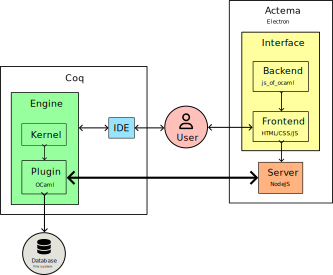
\includegraphics[width=1.3\textwidth]{archi.pdf}
  \caption{Architecture of the \kl{coq-actema} system}
  \labfig{archi}
\end{figure*}

\begin{figure*}
  \includegraphics[width=1.5\textwidth]{coq-actema.png}
  \AP On the left, the usual interactive view of the \kl{proof script}, in the
  \intro{VsCoq} \kl{IDE} \cite{VsCoq}. On the right, the graphical \kl{proof view} of
  \kl{Actema}.
  \caption{ Graphical layout of the \kl{coq-actema} system}
  \labfig{coq-actema}
\end{figure*}

Let us now give the full picture of the \kl{coq-actema} system that integrates
both \kl{Actema} and the \kl{Coq} plugin. A schematic view of its overall
architecture, including the various components and their relationships, is
provided in \reffig{archi}. The different \emph{processes/agents} involved are
represented by shapes of different \emph{colors}, and we add a directed
\emph{arrow} whenever two of them communicate with each other, where the
\emph{source} requests data from or sends instructions to the \emph{target}.

The \process{User} (pink circle) is the only human agent in the system, and
drives all interactions. She interacts with the \kl{Coq} and \kl{Actema}
subsystems (transparent rectangles), through the interfaces provided by her
\kl{Coq} \process{IDE} of choice (blue rectangle) and \kl{Actema}'s
\process{Frontend} (yellow rectangle). This will typically take the form of a
two-windows layout, as depicted by the screenshot of \reffig{coq-actema}.

\subsection{Actema web app}

\AP
The \kl{Actema} web app runs in a process independent from \kl{Coq}, represented
by the yellow \process{Interface} rectangle. We add a third layer to the
\process{Frontend} and \process{Backend} described in \refsec{actema}, namely a
\intro{HTTP} \process{Server} (orange rectangle) that handles requests from, and
responses to the \kl{Coq} \process{Plugin}. Thus we implement interprocess
communication between \kl{Actema} and \kl{Coq} through the network layer of the
operating system, rather than a more local mechanism such as Unix pipelines.
There are a few reasons behind our choice of the \kl{HTTP} protocol:
\begin{itemize}
  \item it provides useful abstractions when working with a client/server
    architecture structured around requests;
  \item it is a widely spread standard, especially in web technologies. Thus we
    were able to reduce development time by reusing generic implementations of
    both client and server from standard libraries;
  \item more anecdotically, this makes it easy to run \kl{Coq} and \kl{Actema}
    on different machines connected on the same network. This could be used for
    instance to offload heavy computations in a proof to the machine running
    \kl{Coq}, while still being able to interact with \kl{Coq} through
    \kl{Actema} on the weaker machine.
\end{itemize}
The \process{Server} runs in a process separate from the \process{Interface}, in
order to avoid any delay in the latter. Then we bundle everything in an
\intro{Electron} application \cite{Electron}, so that \kl{Actema} can easily be
run locally on most operating systems. This also allows us to exploit the
multi-process architecture of Electron \cite{ElectronProcess}, where the
so-called \emph{main} process runs the server and has the ability to issue
system calls for networking through the \intro{Node.js} \kl{HTTP} library
\cite{NodeJS}; and the so-called \emph{renderer} process runs the
\process{Interface} in the \intro{Chromium} browser.

\subsection{\kl{Coq} plugin}

The \process{Plugin} is loaded dynamically in \kl{Coq}'s \process{Engine} (green
rectangle) by executing the following command in a \kl{proof script}:
\begin{minted}[fontsize=\normalsize]{coq}
  From Actema Require Import Loader.
\end{minted}
% This can be done dynamically by the \process{User} in her \process{IDE}, or
% statically at compile time.
It exposes a single \kl{tactic} called \texttt{actema}, which can run in two
distinct modes:
\begin{description}
  \item[\bfseries Interactive] The \process{Plugin} sends the current
  \kl{subgoal}s to \kl{Actema}, and the user applies a sequence of actions on
  them. Each time an action is performed, it is sent back to \kl{Coq}, compiled
  into the appropriate \kl{tactic} call, and then executed to generate new
  \kl{subgoals} that are sent again to \kl{Actema}. The \texttt{actema}
  \kl{tactic} finishes its execution either when:
  \begin{itemize}
    \item all \kl{subgoals} are proved (in \kl{Actema});
    \item the \process{User} decides to stop and give back control to the
    \process{IDE};
    \item in some rare cases, an unrecoverable error occurs.
  \end{itemize}

  \item[\bfseries Non-interactive] If the \texttt{actema} \kl{tactic} has
  already been executed on the \kl{subgoal} under focus, then the
  \process{Plugin} automatically saved the sequence of actions performed by the
  \process{User} in a \process{Database} (gray circle). Currently for ease of
  development, the \process{Database} is implemented as a simple directory on
  the local filesystem, where each file encodes an entry as follows:
  \begin{itemize}
    \item the filename is a hash code that uniquely identifies the \kl{goal} by both
    its \emph{content}, i.e. the statements of the hypotheses and conclusion,
    and an optional \emph{identifier}, which can be given as argument to the
    \kl{tactic} in the form of an arbitrary string;
    \item the contents of the file is a \intro{Base64} encoding of
    the data specifying each action, whose format will be detailed in
    \refsec{compilation}.
  \end{itemize}
  Then the \kl{tactic} will load the sequence of actions from the appropriate file,
  recompile it into one big \kl{tactic}, and execute it on the current \kl{subgoal}.
\end{description}
One can also force the execution in interactive mode by using a variant of the
tactic named \texttt{actema\_force}. We provide details of the complete
interaction protocol followed by the \texttt{actema} \kl{tactic} in the following
section.

\AP
Regarding the implementation of the \process{Plugin}, we chose to do it in the
standard way by interfacing with the \intro{coq-core} API in \kl{OCaml}
\cite{CoqCore}, although it has been encouraged in recent versions of \kl{Coq}
to interface with more stable APIs such as those provided by \intro{Coq-Elpi}
\cite{CoqELPI} and \intro{MetaCoq} \sidecite{MetaCoq}\sidenote{Indeed, breaking
changes are frequently introduced in \kl{coq-core} with newer versions of
\kl{Coq}, which requires more maintenance efforts from plugin developers.}. The
main reason is that our plugin performs \emph{side effects} by interacting with
an external environment: the file system when saving and retrieving graphical
proofs, and the network when issueing \kl{HTTP} requests to \kl{Actema}. Those
cannot be implemented in the aforementioned frameworks.

\section{Interaction protocol}\labsec{protocol}

\begin{figure*}
  \includegraphics[angle=90,height=\textheight]{protocol-1.pdf}
  \vspace{2em}
  \caption{Sequence diagram of \kl{coq-actema}'s interaction protocol ---
  non-interactive mode}
  \labfig{protocol1}
\end{figure*}

\begin{figure*}
  \includegraphics[angle=90,height=\textheight]{protocol-2.pdf}
  \vspace{2em}
  \caption{Sequence diagram of \kl{coq-actema}'s interaction protocol ---
    breaking out of the interaction loop}
  \labfig{protocol2}
\end{figure*}

\begin{figure*}
  \includegraphics[angle=90,height=0.9\textheight]{protocol-3.pdf}
  \vspace{2em}
  \caption{Sequence diagram of \kl{coq-actema}'s interaction protocol ---
    applying an action}
  \labfig{protocol3}
\end{figure*}

\AP
We will now unroll the details of a complete interaction in \kl{coq-actema},
starting from the \process{User} calling the \texttt{actema} \kl{tactic} in her
\process{IDE}, and ending with her viewing the new \kl{subgoals} displayed in
the \process{IDE}. We chose to represent this with a \intro{sequence diagram},
as specified by the \intro{UML} standard \cite{enwiki:1153944336}. This kind of
\kl{diagram} is used to depict runtime behavior of a system, showing
interactions between objects and the messages they exchange in the order they
occur chronologically. In our case, the objects are the different processes
described in the previous section, as well as the \process{User}. Since the full
interaction is quite involved, we split the \kl{diagram} in three parts:
\reffig{protocol1} includes the beginning of the interaction, focusing on the
non-interactive mode of the \texttt{actema} \kl{tactic} where the
\process{Plugin} communicates with \kl{Coq}'s \kl(PA){kernel} and the
\process{Database}. \reffig{protocol2} and \reffig{protocol3} tackle the
interactive mode of the \texttt{actema} \kl{tactic}: \reffig{protocol2} focuses
on the conditions for breaking out of the interaction loop, and
\reffig{protocol3} on the interactions at work when the \process{User} performs
a proof action in \kl{Actema}.

\subsection{Translating goals}

\AP
The first task performed by the \process{Plugin} when calling the
\texttt{actema} \kl{tactic} is to ask the \kl(PA){kernel} for the data of the
\kl{subgoal} $G$ currently under focus. Then for the \kl{goal} $G$ to be
understandable by the \process{Backend} of \kl{Actema}, the \process{Plugin}
will translate it into a new representation $\intro*\trgoal{G}$ in a custom datatype.
In order to share the definition of this datatype across implementations of the
\process{Plugin} and \process{Backend}, we decided to use the \intro{ATD} data
specification language \cite{ATD}. It provides a set of tools to automatically
generate idiomatic datatype definitions in a few target languages --- including
\kl{OCaml} --- along with (de)serialization and validation helpers. This is
particularly fit for our usecase, where we need to serialize complex data like
$\trgoal{G}$ in order to transmit it over \kl{HTTP} messages. Since both the
\process{Plugin} and \process{Backend} are written in \kl{OCaml}, it also allows
us to share across implementations our own domain-specific helpers for
manipulating this data.

\begin{figure}
  \input{listings/atd-fo.tex}
  \caption{\kl{ATD} definitions for \kl{first-order} formulas and environments}
  \labfig{atd-fo}
\end{figure}

\begin{figure}
  \input{listings/atd-goals.tex}
  \caption{\kl{ATD} definitions for \kl{goals}}
  \labfig{atd-goals}
\end{figure}

The \kl{ATD} definition of \kl{goals} is given by the \texttt{goal} type in
\reffig{atd-goals}\sidenote{The syntax is almost the same as that of \kl{OCaml}
datatypes, for the reader already acquainted with this language.}. It relies on
the \kl{ATD} types \texttt{form} of \emph{formulas}, and \texttt{env} of
\emph{environments} of available constants and variables. In our setting, these
correspond respectively to the formulas and \emph{signatures} of many-sorted
\kl{FOL}, whose \kl{ATD} definitions are given in \reffig{atd-fo}. But
one could imagine using formulas and environments in \kl{higher-order} logic
instead, and this would not change the structure of the \texttt{goal} datatype.
Note that hypotheses are encoded with a \texttt{h\_id} attribute corresponding
to their string identifier in the \kl{Coq} \kl{goal}, even though we do not
display it in \kl{Actema}'s interface. This is required later by the plugin to
compile actions into \kl{tactics}, because we need to identify which \kl{Coq}
hypotheses correspond to those designated graphically by the \process{User}.

\subsection{Retrieving actions}

\AP
The next step for the \process{Plugin} is to check if there already exists a
graphical proof associated to $\trgoal{G}$ in the \process{Database}. If so,
then it retrieves it in the form of a list $A$ of \emph{actions}, whose data
format will be precised in \refsec{compilation}. There is also a positive
integer $n_i$ associated to each action $A_i$ in the list, corresponding to the
index of the \kl{goal} to which $A_i$ applies in the list of \kl{subgoals}. Then
each $A_i$ is compiled into a \kl{tactic} $\intro*\traction{A_i}$, and all the
$\traction{A_i}$ are composed into a unique \kl{tactic} $\tau$, which is
executed by the \kl(PA){kernel} on $G$ to apply the full sequence of actions.

\begin{remark}
  Currently the translation $\trgoal{\cdot}$ is not \emph{injective}: it might
  map two different \kl{Coq} \kl{goals} to the same \kl{Actema} \kl{goal},
  because strictly \kl{higher-order} subterms are translated into a
  \texttt{dummy} atomic predicate/function. Thus one might retrieve a proof from
  a different \kl{goal} when calling the \texttt{actema} \kl{tactic}. However
  this is not problematic, since the \process{User} cannot perform any actions
  involving the parts of the two goals that make them distinct; they might as
  well be seen as the same \kl{goal} from her point of view. It can thus be
  considered as a feature that maximizes proof reuse.
\end{remark}

If there is no saved proof for $\trgoal{G}$, then the \texttt{actema}
\kl{tactic} has never been executed on $\trgoal{G}$, and thus we let the
\process{User} provide a (partial) proof in \kl{Actema}. First the
\process{Plugin} retrieves the list $Gs$ of all \kl{subgoals}, instead of just
the one under focus. If $Gs$ is empty, which would happen after all subgoals
have been solved from \kl{Actema}, then it sends a \request{QED} request to
\kl{Actema} so that the latter can update its view accordingly, and the
interaction loop with \kl{Actema} stops here\sidenote{In \reffig{protocol2} and
\reffig{protocol3}, we depict requests as being sent to the \process{Frontend}
of \kl{Actema}. This is an imprecision for trading in some readability, since as
reviewed in \refsec{architecture} it is the \process{Server} which handles
communication with the \process{Plugin}, and in particular forwards requests to
the \process{Frontend}.}.

\AP
If $Gs$ is not empty then there is at least one \kl{subgoal}, and we send an
\request{action} \kl{HTTP} request to \kl{Actema}, whose body contains the
translated \kl{subgoals} $\trgoal{Gs}$. To do this, we chose to serialize
$\trgoal{Gs}$ with the \intro{Biniou} helpers autogenerated by \intro{atdgen},
the \kl{OCaml} backend of \kl{ATD}. According to its authors: ``Biniou is a
binary format extensible like JSON but more compact and faster to process''
\cite{atdgen}. This data is then deserialized and compiled into a set
$\mathcal{G}$ of \kl{HTML} \intro{DOM} nodes by the \process{Backend}, so that
the goals can be rendered by the \process{Frontend} and exposed to the
\process{User}. Then the \process{User} has two options:
\begin{itemize}
  \item she can apply either a click, \kl{DnD} or \kl{contextual
  action}\sidenote{See \refsec{funcs} for an introductory example of
  \kl{contextual action} with \kl{Unfold}.}. The precise protocol followed for
  applying an action is summarized in \reftab{action-protocol}. Let us focus on
  the more complex case of \kl{DnD} actions. The \textbf{Start} column describes
  how the \process{User} \emph{starts} the action, here by dragging some
  \kl{item} $I$ of the current \kl{subgoal}. Then the \process{Frontend} asks
  the \process{Backend} for the set $\mathcal{A}$ of all available \kl{DnD}
  actions involving $I$. The \textbf{Selection} column describes how the
  computation of $\mathcal{A}$ is impacted by the set $S$ of subterms that are
  selected in the current \kl{subgoal}. For \kl{DnD} actions, we essentially
  filter out all \kl{linkages} that do not match the selection. The
  \textbf{Render} column describes how $\mathcal{A}$ is \emph{rendered} to the
  \process{User}: here we highlight the set $Q$ of all \kl(sfl){valid} drop
  targets, which correspond to subterms of the current \kl{goal} located in
  other \kl{items}\sidenote{Highlighting is here understood in a \emph{visual}
  sense: in the current implementation of \kl{Actema}, subterms are indicated
  graphically by squaring them. But one could imagine other modalities for
  highlighting, typically \emph{spelling} the subterms with a speech synthesis
  algorithm, e.g. for users with impaired vision.}. Lastly, the \textbf{End}
  column describes how the user chooses a specific action $A \in \mathcal{A}$ to
  apply, here by dropping $I$ on a given target $q$. Then $A$ is serialized and
  sent in the body of the response to the \request{action} request, together
  with the index $n$ of the \kl{subgoal} under focus in \kl{Actema}. The
  \process{Plugin} can therefore compile $A$ into a \kl{tactic} $\traction{A}$
  which is executed on the $n^{\text{th}}$ Coq \kl{subgoal}, giving a new list
  of \kl{subgoals} which is sent again to \kl{Actema} for another round of the
  interaction loop.

  \item or she can click on a \texttt{Done} button in \kl{Actema}'s interface:
  this has the effect of answering the \request{action} request from the
  \process{Plugin} with a \request{done} response, and the interaction loop with
  \kl{Actema} stops here. This will happen when the \process{User} wants to go
  back to editing the \kl{proof script}, either because she is satisfied with
  the new \kl{subgoals} obtained from previous actions, or because she is stuck
  and wants to try native \kl{Coq} \kl{tactics} instead. Indeed our protocol is
  \emph{synchronous}: the \process{IDE}'s interface is stuck until the
  \texttt{actema} \kl{tactic} has finished its execution, and thus one cannot
  edit the \kl{proof script} \emph{and} build a proof in \kl{Actema} at the same
  time.
  % \sidenote{This is because the
  % \emph{document checking model} of most \kl{Coq} IDEs is itself synchronous: when
  % the \process{User} modifies the \kl{proof script} at a location before the current
  % execution point, the proof state goes back to how it was at that location, and
  % every command/tactic coming after it needs to be reinterpreted.}
\end{itemize}

\begin{table*}[]
  \def\arraystretch{1.5}
  \begin{tabular}{|c|C{0.2\textwidth}|C{0.4\textwidth}|C{0.25\textwidth}|C{0.2\textwidth}|}
  \hline
  \textbf{Kind} & \textbf{Start}       & \textbf{Selection $S$} &
  \textbf{Render}                      & \textbf{End} \\ \hline
  Click         & Hover \kl{item} $I$       & Ignored & Highlight $P \subseteq
  \subterms{I}$ & Click on some $p \in P$    \\ \hline
  \kl{DnD}           & Drag \kl{item} $I$        &
      If $\exists p \in S \cap \subterms{I}$ then match only $p \link q$ where
      $q \in \substermscompl{\subterms{I}}$
      \newline
      If $\exists q \in S \cap \substermscompl{\subterms{I}}$ then match only $p
      \link q$ where $p \in \subterms{I}$
    & Highlight $Q \subseteq \substermscompl{\subterms{I}}$ & Drop on some $q \in Q$ \\ \hline
  Contextual    & Open menu & Populate menu only with actions
  applicable on $S$ & Show menu & Choose an \kl{item} in the menu \\ \hline
  \end{tabular}
  \raggedright
  \parbox{\textwidth}{
    \vspace{1.5em}
    We introduced some notations for conciseness:
    \begin{itemize}
      \item $p, q$ denote \kl{paths} to subterms of the current goal
      \item $P, Q$ and the selection $S$ denote sets of \kl{paths}
      \item $\intro*\subterms{I}$ denotes the set of \kl{paths} within \kl{item} $I$
      \item $\substermscompl{\subterms{I}}$ denotes the complement of $\subterms{I}$, i.e.
      all \kl{paths} in all \kl{items} $J \not= I$
      \item $p @ q$ is a \kl{linkage} as introduced in \refsec{linkages}
    \end{itemize}}

  \caption{Protocol for applying an action in Actema}
  \labtab{action-protocol}
\end{table*}


\section{Compiling actions}\labsec{compilation}

Once the \process{Plugin} has received the actions to execute, either from the
\process{Database} or the \process{User}, it will compile them with the function
$\traction{\cdot}$ which translates any action $A$ into a \kl{Coq} tactic
$\traction{A}$. This function actually has access to some other data: \kl{Coq}'s
\kl{goal} $G$, its \kl{Actema} translation $\trgoal{G}$, and a bijective mapping
$\Sigma$ between \kl{Coq} constants in the environment of $G$ and the
corresponding \kl{Actema} symbols in the \kl{first-order} signature of
$\trgoal{G}$.

\subsection{The \texttt{action} datatype}

\begin{figure}
  \input{listings/atd-actions.tex}
  \caption{\kl{ATD} definitions for actions}
  \labfig{atd-actions}
\end{figure}

The \texttt{action} datatype is described thoroughly in the \kl{ATD} specification
provided in \reffig{atd-actions}. It is a big algebraic datatype, where each
constructor encodes a specific \emph{type} of action. An action's type is
equivalent to the \emph{signature} of a \kl{tactic}, i.e. its name and the types
of its arguments. In particular, the translation function $\traction{\cdot}$ is
defined as a big pattern-matching on the action's type\sidenote{Note that an
action's type is orthogonal to what we referred to as its \emph{kind} in
\reftab{action-protocol}, that is the interface mechanism through which it is
accessible. One might for example want to map some action types to \emph{vocal
commands} instead of click or \kl{DnD} gestures.}. The arguments in action types
rely on most datatypes defined previously in \reffig{atd-fo} and
\reffig{atd-goals}, and on two new datatypes: the type \texttt{ipath} of
\emph{\kl{paths}}, which is used pervasively to designate subterms of the current
\kl{subgoal} (that are typically indicated by the \process{User} through
pointing); and the type \texttt{itrace} of \emph{\kl{subformula linking}
traces}, which is used in the compilation of \kl{DnD} actions that perform
\kl{subformula linking}, to be described soon.

Most click and \kl{contextual actions} have a straightforward translation as \kl{Coq}
tactics. For instance, the \texttt{AIntro} action that corresponds to a click on
the conclusion $C$ will be mapped to the \kl{Coq} \kl{tactic} that introduces
the main connective of $C$, and is thus defined by case on the latter:
\texttt{intro} for $\limp$ and $\forall$, \texttt{split} for $\land$, etc. The
actions \texttt{AInd}, \texttt{ASimpl} and \texttt{ARed} correspond respectively
to the \kl{contextual actions} \kl{Induction}, \kl{Simplify} and
\kl{Unfold} introduced in \refch{advanced}, and are mapped almost directly
to the equivalent \kl{Coq} \kl{tactics} \texttt{induction}, \texttt{simpl} and
\texttt{red}. The only difference is that they have a \emph{\kl{deep inference}}
flavor, since they can all be applied on an arbitrary subterm selected by the
\process{User}. This relies on our implementation of \kl{deep inference}
semantics directly in \kl{Coq}, that we now briefly describe.

\subsection{Deep inference semantics}

\AP
In a \kl{deep inference} setting, one can reason on subterms located arbitrarily
\emph{deep} inside statements, usually by applying some kind of \kl{rewriting
rules} on them. In particular, the semantics of \kl{DnD} actions described in
\refch{sfl} are based on the rules of \kl{SFL} (\reffig{DISL}). To implement
them, we chose to do a \intro{deep embedding} of \kl{FOL} inside \kl{CoIC}. Here
the word ``deep'' has a different meaning, related to the fact that we encode
the statements of \kl{FOL} with our own custom datatypes, instead of reusing the
statements of \kl{CoIC}. This makes it easier to define the \kl{SFL}
\kl{rewriting rules}, in particular because we need to manipulate
\emph{\kl{contexts}} (\refdef{formula-context}) explicitly, and those are not
available for \kl{CoIC} propositions.

\AP
Then we use a technique called \intro{computational reflection} in order to
apply the embedded \kl{deep inference} semantics to \kl{Coq} \kl{goals}.
Originating from the \emph{small scale reflection} methodology supported by the
{\kl{\ssreflect}} framework \cite{SSR}, it consists in:
\begin{enumerate}
  \item translating \kl{Coq} objects into their equivalent formulation in the
\kl{deep embedding} with a \texttt{reify} function;
  \item reasoning on the \kl{deep embedding} with the help of \kl{Coq} programs
(also called \emph{fixpoints});
  \item translating objects back into \kl{Coq} with a \texttt{reflect} function.
\end{enumerate}
\AP
It is easy to implement the \texttt{reflect} function because the datatypes in a
\kl{deep embedding} are almost always defined as \emph{inductive} \kl{types},
and thus one can easily do pattern-matching on them. It is a different story for
the \texttt{reify} function, especially in our case: indeed we want to translate
the statements of \kl{Coq} \kl{goals} into \kl{first-order} propositions. But
\kl{Coq} statements are objects of \kl{type} \texttt{Prop}, and thus cannot be
pattern-matched on inside \kl{CoIC}\sidenote{For reasons of \kl{consistency} of
the logic, well-known in the literature on \kl{type theory}.}. Thus we need to
have recourse to a \emph{meta-programming} language in order to inspect the
structure of \kl{Coq} \kl{goals}. Here we use the standard \intro{Ltac}
language, which provides powerful constructs for pattern-matching on
\kl{goals}\sidenote{A downside of \kl{Ltac} is that it is an \emph{untyped}
language, whose programs are notoriously hard to debug and maintain. One might
consider a cleaner implementation with more recent alternatives in the \kl{Coq}
ecosystem, such as the successor to \kl{Ltac} \intro{Ltac2} \cite{Ltac2}, or the
\kl{MetaCoq} project \cite{MetaCoq}.}.

The most complex \kl{tactics} are those implementing \kl(dnd){backward} and
\kl(dnd){forward} \kl{DnD} actions, called respectively \texttt{backward} and
\texttt{forward}. They rely on two \kl{Coq} fixpoints \texttt{b3} and
\texttt{f3} which respectively compute the new conclusion $\mathtt{b3}(p, q, T)$
from a \kl(dnd){backward} \kl{linkage} $p \back q$, and the new hypothesis
$\mathtt{f3}(p, q, T)$ from a \kl(dnd){forward} \kl{linkage} $p \forw q$, where
$T$ is the so-called \emph{\kl{subformula linking} trace} mentioned earlier. Of
course the \kl{paths} $p, q$ and the trace $T$ are all expressed with custom
\kl{Coq} datatypes relying on our \kl{deep embedding} of \kl{FOL}. The role of
the trace in particular is to provide the list of \kl{SFL} \kl{rewriting rules}
to apply, as well as the \kl{Coq} \kl{terms} instantiating quantifiers that were
computed in \kl{Actema} by \kl{unification} of the two linked subformulas. Then
we formulate in \kl{Coq} two theorems that guarantee the logical
\emph{soundness} of \texttt{b3} and \texttt{f3} (\reffig{dnd-snd}),
corresponding to \refthm{sfl-soundness}. Note that the theorems are formulated
using the native implication connective \texttt{->} of \kl{Coq}, thanks to the
\texttt{reflect} function. The final \kl{tactics} \texttt{backward} and
\texttt{forward} can thus modify the \kl{goal} by applying these theorems, first
reifying the \kl{goal} with the \texttt{reify} function, and then relying on the
fact (also proved in \kl{Coq}) that \texttt{reflect} is the inverse of
\texttt{reify}.

\begin{figure}
  \begin{minted}
  [
  frame=lines,
  framesep=2mm,
  baselinestretch=1,
  fontsize=\footnotesize,
  linenos
  ]
  {coq}

Theorem b3_corr : forall p q T,
  coerce p -> coerce (b3 p q T) -> coerce q.

Theorem f3_corr : forall p q T,
  coerce p -> coerce q -> coerce (f3 p q T).

\end{minted}

  \caption{Soundness theorems of \kl{DnD} fixpoints in \kl{Coq}}
  \labfig{dnd-snd}
\end{figure}

% \begin{theorem}[Soundness of \kl{DnD} fixpoints]~\\
%   $$\forall p.\ \forall q.\ \forall T.\ \mathtt{reflect}(p) \limp
%   \mathtt{reflect}(\mathtt{b3}(p, q, T)) \limp \mathtt{reflect}(q)$$
%   \center{and}
%   $$\forall p.\ \forall q.\ \forall T.\ \mathtt{reflect}(p) \limp
%   \mathtt{reflect}(q) \limp \mathtt{reflect}(\mathtt{f3}(p, q, T))$$
% \end{theorem}

\begin{remark}
  There exist a few other approaches to the computer implementation of \kl{deep
  inference} systems. Ozan Kahramanoğulları has pioneered the field, by
  implementing various \kl{calculi of structures} inside frameworks like Maude
  \cite{kahramanogullari_maude_2008} and Tom
  \cite{kahramanogullari_implementing_2005}, that are dedicated to the
  specification of \kl{rewriting systems}. For an integration within modern
  \kl{proof assistants}, we only know of Chaudhuri's recent work
  \sidecite{chaudhuri_certifying_2022} that explores different techniques in
  addition to reflection, like \emph{combinators} and some more powerful usages
  of \emph{metaprogramming}. He also provides an effective implementation of the
  techniques in his \kl{Profint} tool \cite{DBLP:conf/cade/Chaudhuri21}, that
  allows to export \kl{subformula linking} derivations built with \kl{Profint}'s
  \kl{GUI} as \kl{proof scripts} directly executable in various \kl{proof
  assistants} (\kl{Coq}, \kl{Lean}, \kl{Isabelle/HOL}).
\end{remark}

\section{Future works}\labsec{pluginfuture}

The \kl{coq-actema} system described in this chapter has been successfully
implemented and tested on various simple examples, including those of
\refsec{edukera} and \refsec{arith}. But there are many \kl{Coq} \kl{goals} that
cannot be properly handled in \kl{Actema}, which still hinders the usability of
the system in real mathematical developments, even in an educational setting.
Typically, the example of \refsec{funcs} cannot be completely performed in
\kl{Actema}, in this case because of the lack of support for
\emph{\kl{higher-order}} functions and predicates, but also because of the poor
support for user-defined \emph{notations}. Those are only a few of the current
limitations of \kl{coq-actema}, and we describe in the following pages how they
could be overcome, both to widen the scope and improve the \kl{UX} of the
system.

\subsection{Higher-order logic}

The importance of being able to express and manipulate \kl{higher-order}
functions and predicates has been stressed multiple times before. The fact that
\kl{Actema} is limited to \kl{first-order logic} is mostly a historical
contingency, motivated by the fact that some algorithms like \kl{unification}
are more tractable in this setting. But now that we rely on \kl{Coq}'s proof
engine, there is no fundamental reason for maintaining this choice. Because the
language of statements is at the foundation of a logical framework, many other
components of a \kl{proof assistant} will depend on it. Thus the switch to
\kl{higher-order} logic should be done as soon as possible, to limit the amount
of refactoring work to perform in the future. This will require changes to
\kl{Actema}'s \process{Backend} and \process{Frontend}, but also to the \kl{Coq}
\process{Plugin}\sidenote{The \kl{Coq} theory implementing the tactics for
\kl{deep inference}-based actions already has partial support for
\kl{higher-order} \kl{goals}, thus work remains mostly on the side of the
translation module for \kl{Actema} written in \kl{OCaml}.} and the \kl{ATD}
datatype definitions enabling communication between the two.

One central question in the transition to \kl{higher-order} logic is how
\kl{unification} of subterms will be handled. Algorithms in this setting are
known to be incomplete because of undecidability
\sidecite{huet_undecidability_1973}, and their implementation can be very
tricky. The most sensible option seems to rely on the implementation already
provided by \kl{Coq}, which is the fruit of years of development and
improvements. But this would require changing the interaction protocol of
\kl{coq-actema}, by allowing the \process{Backend} of \kl{Actema} to make
\kl{unification} requests to the \process{Plugin}. This might be doable without
changing the current client-server architecture, but will probably involve some
intricate design decisions.

A more radical solution would be to replace the \request{actions} request from
the \process{Frontend} to the \process{Backend} by a \texttt{start} response
from the \process{Frontend} to the \process{Plugin}, with the data of the
selection in its body. Then we could completely delegate the computation of
available actions to the \process{Plugin}, allowing us to freely use \kl{Coq}'s
\kl{unification}. This might not be too hard since we should be able to directly
reuse \kl{OCaml} code from the \process{Backend}, but is a deeper structural change
to the interaction protocol, that makes the \process{Plugin} responsible for an
important part of \kl{Actema}'s behavior. And this would induce a lot of
unnecessary reimplementation efforts if we were to port the \process{Plugin} to
other \kl{PAs}.

\subsection{Notations}

Another big limitation already mentioned in the introduction of this chapter, is
that we do not handle custom \emph{notations} for displaying
terms\sidenote{Apart from expressions in Peano arithmetic, for which we have ad
hoc support.}. It is however a crucial feature for making proofs in a specific
domain tractable, especially in the \kl{PbA} paradigm where one needs to
manipulate directly statements in the \kl{goal}. Now that we are connected to
\kl{Coq}, we can in principle reuse the notation system already implemented
within \kl{Coq}. The \kl{coq-core} \kl{OCaml} API indeed exposes methods for
pretty-printing \kl{Coq} terms using their assigned notations. The problem is
that these methods only return \emph{strings}, but in order to manipulate
\kl{terms} interactively in \kl{Actema} we also need access to \emph{trees}
mapping their subterm structure to the pretty-printed string. At the time of
writing there is no support for the latter, but the \kl{Coq} development team
informed us that they plan to add this feature. The same problem was met by the
developers of the \kl{ProofWidgets} framework in \kl{Lean}, and they had to
modify the pretty-printer of \kl{Lean} upstream\sidenote{Section 4.1 of
\cite{ayers_graphical_2021}.}.

Once one has support for custom notations displayed in an \kl{HTML} page, it is
tempting to also allow for arbitrary \kl{HTML}/\kl{JS} code, instead of just
textual notations. This opens the space for very rich graphical and interactive
representations of mathematical objects, which could greatly improve the
accessibility of \kl{PAs}, but also their expert usage by enabling
domain-specific interfaces targetting non-standard methods of reasoning. A
typical example is the \emph{\kl{diagrammatic}} reasoning pervasive in
\emph{category theory}, which is very hard and cumbersome to express as
manipulation of logical statements. Actually a system very similar to
\kl{coq-actema} is currently being developed by Luc Chabassier \cite{LucTalk},
for the very purpose of integrating \kl{diagrammatic} proofs in category theory
to the traditional \kl{proof script} workflow. One could imagine in the
long-term embedding this system as a subsystem of \kl{coq-actema}, through an
advanced protocol for interactive notations.

In fact the \kl{ProofWidgets} framework has been designed with this usecase in
mind from the outset. But they rely on a very different architecture compared to
that of \kl{coq-actema}, where the methods generating the \kl{HTML}/\kl{JS} code
of pretty-printed \kl{terms} are directly implemented in a DSL embedded in the
meta-programming language of the \kl{PA}. While this allows easy access to all
meta-programming facilities for manipulating \kl{terms}, this makes their
framework only usable within \kl{Lean}, while \kl{Actema} could in principle be
used with any \kl{PA} that implements a corresponding plugin (for example with a
\texttt{lean-actema} variant of our system).

\subsection{Lemma search}

We already described in \refsec{funcs} the \emph{lemma search} feature of
\kl{Actema}. Currently it is implemented only in its standalone version. Adding
support for it in \kl{coq-actema} would require additional efforts compared to
other \kl{contextual actions} like \kl{Induction}. Indeed we do not only need
access to the current \kl{goal}, but also to the full global environment of
\kl{Coq} where lemmas are stored. While in the standalone version we had a toy
lemma database with very few entries, the standard library of \kl{Coq} contains
thousands of lemmas. And to use our selection-based filtering algorithm
implemented in \kl{Actema}, we would need to translate the entire library into
statements understandable by \kl{Actema}'s \process{Backend}, and then send it
over \kl{HTTP}. Thus it will be important to implement some cache mechanism to
remember which lemmas have already been exported to \kl{Actema}'s own database,
to avoid recomputing the translation each time.

% \subsection{Tighter IDE integration}

% Design a new architecture/protocol that supports \emph{continuous, incremental
% document checking} (typically by inserting tactic calls in the \kl{proof script}
% for each action, maybe coq-lsp can do that?)

\subsection{Proof evolution}\labsubsec{proof-evolution}

\AP
An important question when designing a proving environment is how users will be
able to manipulate an \emph{existing} (partial) proof, either one they have
built in the past, one that was built by other people, or a mix of both in a
collaborative context. This is a complex problem spanning various activities
that are involved in the lifecycle of a proof: modifying it while it is being
constructed; reading it for the first time, or many months/years after it was
written; updating it after slight changes to the statement of its theorem;
etc\sidenote{Not very surprisingly, those activities are commonly found in the
context of \emph{programming} environments. Thus one might get insight by
cross-pollinating ideas from both domains, in the spirit of the \kl{Curry-Howard
correspondence} (which also underlies the design of \kl{Coq}).}.

\begin{digression}
One might even argue that thinking about the best way to \emph{represent} a
proof leads to more fundamental questions, that have been much debated both in
\kl{proof theory} and the history and philosophy of mathematics: what is the
essence of a proof, seen as a meta-mathematical object
\cite{strasburger-problem-2019}? What are the roles played by informal and
formal proofs, both in the teaching of mathematics, and the social and
scientific practice of mathematicians \cite{bartzia:hal-04087080}?
\end{digression}

In the literature and community of people designing \kl{proof assistants}, these
various problematics are generally regrouped under the term of \intro{proof
evolution}. A fundamental remark about the \kl{PbA} paradigm, and thus about the
\kl{coq-actema} system, is that it has not been designed with \kl{proof
evolution} in mind from the outset. Indeed, a proof built with the
\texttt{actema} \kl{tactic} will provide the least possible amount of information in
the \kl{proof script}, since we can just witness the call to that \kl{tactic}. And
currently there are no facilities to visualize the associated sequence of
actions stored in the \process{Database} of graphical proofs.

The first question that should be answered is: how do we represent statically a
sequence of graphical actions, let alone a single action? For a machine
representation, we can just dump the data of the action invokation, and this is
indeed what we do with the \process{Database}. But finding a human-readable
representation that an average user can quickly manipulate and reason about is a
lot more delicate. The most direct way may be to abandon text altogether, and
just replay the action on the interface through a graphical \emph{animation}.
This is an intrisically temporal and dynamic representation, akin to a
mathematician unfolding her demonstration on the blackboard. One could then
imagine an interface dedicated to richly-structured navigation inside this
sequence of animations, in the style of an improved video player.

A more conservative solution would be to find a systematic way to translate a
sequence of actions into a proof text. The question of generating
\kl{declarative} proof texts from \kl{imperative} \kl{proof scripts} has already
been explored by some authors, especially in the case of proofs expressed in
natural language\sidenote{See for example section 3.6 of E. Ayers' thesis
\cite{ayers_thesis}. We can also mention ongoing work of Patrick Massot in the
\kl{Lean} \kl{proof assistant} \cite{LeanIPAM}.}. Our hope is that the structure
of proofs in the \kl{PbA} paradigm might be well-suited to the generation of
readable and concise proof texts, thanks notably to the \kl{subformula linking}
semantics of \kl{DnD} actions that exhibit clearly the flow of argumentation.

An even more pragmatic solution, that should be straightforward to implement in
the short-term, consists in inserting \kl{tactic} invokations in the \kl{proof script}
that are in one-to-one correspondence with graphical actions. Since we actually
compile actions into \kl{tactics}, this is in principle easy to implement. However,
there are currently two drawbacks to this approach:
\begin{description}
  \item[Leaking SFL data] Since most \kl{tactics} are \kl{deep inference}-based,
  they take as arguments the \kl{paths} to manipulated subterms, in the form of
  lists of integers. Those are hard to read by humans, and very sensible to
  small changes in the shape of the \kl{goal}. This is even worse for the
  \texttt{backward} and \texttt{forward} \kl{tactics}, because they also take as
  argument the \kl{subformula linking} trace, which is a very complex data
  structure expressed in our \kl{deep embedding} of \kl{FOL}, and hence should
  not leak into the user interface. Hopefully, relying on \kl{Coq}'s
  \kl{unification} instead of \kl{Actema}'s should mitigate the complexity of
  the trace, by removing the need to incorporate full substitutions. There is
  also the possibility of replacing integer-based \kl{paths} by \emph{patterns}
  in the {\kl{\ssreflect}} language, which are known to be a more robust way to
  designate subterms. But this would require the design of some clever
  algorithm, able to generate patterns that correctly generalize the
  \process{User}'s intent from the sole data of selected \kl{paths}.

  \item[Editor integration] The interaction protocol described in
  \refsec{protocol} does not provide any way to send requests to the
  \process{IDE}, which would be necessary to actually insert the \kl{tactic}
  invokation at the right location in the \kl{proof script}, and this as soon as
  the action is performed by the \process{User}. A ``brutal'' solution would be
  to reimplement \kl{coq-actema} as an extension of a specific \kl{IDE},
  typically \kl{VsCoq} which is also based on web technologies. But this would
  require some big implementation efforts, in addition to locking the
  \process{User} into this specific \kl{IDE}. A better option might be to
  directly interact with a \emph{language server} implementing the Language
  Server Protocol (\intro{LSP}) \cite{LSP}. The \intro{coq-lsp} project aims to
  provide such a server for \kl{Coq}, but at the time of writing of this thesis
  does not implement yet all methods of the \kl{LSP} standard. The one that
  interests us in particular is the \texttt{textDocument/codeAction} method, for
  which support is currently planned \cite{coq-lsp-proto}. Then \kl{coq-actema}
  would stay compatible with all \kl{IDEs} that run \texttt{coq-lsp}.
\end{description}

\pagelayout{wide} % No margins
\addpart{Iconic Manipulations}
\pagelayout{margin} % Restore margins

% % !TEX root =index.tex
\setchapterpreamble[u]{\margintoc}
\chapter{Asymmetric Bubble Calculus}
\labch{bubbles}

\epigraph{Leibniz sought to make the form of a symbol reflect its content. ``In
signs,'' he wrote, ``one sees an advantage for discovery that is greatest when
they express the exact nature of a thing briefly and, as it were, picture it;
then, indeed, the labor of thought is wonderfully diminished.''}
{\textbf{Frederick Kreiling}, \textit{Leibniz}, 1968}


\begin{scope}\knowledgeimport{bubble}


We introduce a new kind of \kl{nested sequent} \kl{proof system} dubbed
\intro{bubble calculus}. Inspired by the \emph{membrane} mechanism of the
\intro{chemical abstract machine} (\reintro{\cham})
\sidecite[5em]{berry_chemical_1989}, so-called \emph{\kl{bubbles}} internalize
the notion of \kl{subgoal} inside \kl{sequents}, rather than through the tree
structure induced by traditional \kl{inference rules}. This allows for a more
hierarchical representation of the \kl{proof state}, where
\kl(sequent){contexts} can be shared between different \kl{subgoals}. In
addition to the usual textual syntax, the \kl{bubble calculus} can be expressed
in a graphical syntax, where logical meaning is captured by \emph{physical}
constraints on \kl{diagrammatic} manipulations, instead of \emph{virtual}
restrictions on available \kl{inference rules}.

% We introduce a new kind of nested sequent \kl{proof systems} dubbed \emph{bubble
% calculi}. Inspired by the \emph{membrane} mechanism of the chemical abstract
% machine ({\cham} hereafter) \sidecite[25em]{berry_chemical_1989}, so-called
% \emph{bubbles} internalize the notion of \emph{subgoal} inside sequents, rather
% than through the tree structure induced by \kl{inference rules}. This allows for a
% more hierarchical representation of the proof state, where contexts can be
% shared between different subgoals. In addition to the usual textual syntax,
% bubble calculi can be expressed in a graphical syntax, where logical meaning is
% captured by \emph{physical} constraints on diagrammatic manipulations, instead
% of \emph{virtual} restrictions on available \kl{inference rules}. In the chemical
% metaphor, \emph{intuitionism} is then characterized as the phenomenon of
% \emph{repulsion} between objects that have the same polarity.

We start in \refsec{chemical} with the genesis of the idea of \kl{bubble
calculus}, coming from the observation that our \kl{Proof-by-Action} paradigm
(\refch{pba}) lends itself quite naturally to a \kl{metaphorical}
interpretation, where actions are seen as \emph{chemical} reactions. In
\refsec{bubbles} we introduce the concept of \emph{bubble} as a way to control
the scope of hypotheses inside \kl{nested sequents} that we call
\emph{\kl{solutions}}. In \refsec{asymmetric} we describe our \kl{proof system} for
\kl{intuitionistic} logic dubbed \emph{asymmetric \kl{bubble calculus}}, based
on multiset \kl{rewriting rules} over \kl{solutions} comprising at most one
conclusion. Finally in \refsec{bubbles-pba}, we import ideas from this
\kl{bubble calculus} back to the realm of \kl{GUIs} for interactive proof
building, analyzing their possible impact for \kl{UX} improvements.

\section{The chemical metaphor}\labsec{chemical}

The \kl{Proof-by-Action} paradigm introduced in \refch{pba} offers multiple ways to
the user to attack the proof of a theorem. \kl{DnD} actions for \kl{subformula linking}
and equality rewriting are the main mechanism, but they only work in a goal
comprising multiple \kl{items}. Since it is customary in \kl{proof assistants} to specify
the \kl{goal} to be proved as a single logical formula, one needs a way to decompose
it into many \kl{items} for further processing through \kl{DnD}. This is precisely what
the \kl{introduction rules} for logical connectives in \kl{sequent calculus} do, and
following the \kl{Proof-by-Pointing} paradigm \cite{PbP} we map them to click
actions (see \refsec{clicks}).

So visually, a proof in \kl{Actema} consists in breaking logical \kl{items} into
subitems positioned freely in space, and then bringing those subitems together
to make them interact and produce a new \kl{item}. This is quite evocative of a
\emph{chemical reaction} controlled by the user, where logical formulas are akin
to molecules made of propositional atoms linked together by logical
connectives\sidenote{This precise \kl{metaphor} about the molecular structure of
propositions can already be found in Russell's introduction to Wittgenstein's
\textit{Tractatus Logico-Philosophicus} \cite[p.~11]{tractatus}, which was the
main inspiration to his philosophy of \emph{logical atomism}
\cite{klement_russells_2020}. Even earlier in the history of logic, C. S. Peirce
took inspiration from chemical \kl{diagrams} to devise his \emph{\kl{existential
graphs}} --- see \cite[pp.~17--18]{Roberts+1973} or our own presentation in
\refsec{beta} for more details.}. Click actions are then a mean to ``heat''
molecules to the point of breaking these chemical bonds. The most canonical
examples are the \kl{right introduction rule} for implication \kl{{\limp}R},
which breaks a conclusion/\kl{positive} \kl{ion} into a new
hypothesis/\kl{negative} \kl{ion} and a new conclusion; and the \kl{left
introduction rule} for conjunction \kl{\land L}, which breaks a hypothesis into
two hypotheses. In fact, we strongly conjecture that these are the only click
actions needed to obtain a complete deductive system for propositional logic:
breaking red implications allows for \kl(dnd){backward} \kl{DnDs}, and blue
conjunctions for \kl(dnd){forward} \kl{DnDs}\sidenote{In \kl{predicate logic},
one would also need the \kl[right introduction rule]{right} (resp. \kl[left
introduction rule]{left}) introduction rule for $\forall$ (resp. $\exists$). It
might also be the case that \kl(dnd){backward} \kl{DnDs} alone are sufficient
for completeness, since a \kl{linkage} of the form $A \back \select{B} \limp C$
will involve a \kl(dnd){forward} phase. In this case only the \kl{right
introduction rules} for $\limp$ and $\forall$ would be required.}.
% \sidenote{Interestingly,
% those rules are the basis for the adjunction between $\land$ and $\limp$ in the
% interpretation of IPL into cartesian closed categories.}

Rather than completeness, the issue here is \emph{consistency} of the user
interface: if the user is allowed to decompose red $\conc{\limp}$ and blue
$\hypo{\land}$, she will assume naturally that she can also decompose blue
$\hypo{\limp}$ and red $\conc{\land}$, as well as $\lor$ of any color. While red
$\conc{\lor}$ can be handled by pointing directly at the disjunct to be proved,
other configurations correspond to rules of \kl{sequent calculus} with multiple
premisses. In \kl{Actema}, this corresponds to creating a new \kl{subgoal} for
each premise, where \kl{subgoals} are displayed one at a time in different
\emph{tabs}: this new interface mechanism breaks the chemical \kl{metaphor}. The
root cause lies in the way \kl{sequent calculus} implements
\emph{context-scoping}: each \kl{subgoal} will share the same initial context of
hypotheses, but future hypotheses ``buried'' in the conclusions must be
available only in their respective \kl{subgoals}. The tabs mechanism implements
this by forcing the user to focus on exactly one tab/\kl{subgoal}, thus making
it impossible to display \kl{items} from different \kl{subgoals} on the same
screen: this renders interaction between items \emph{physically} impossible.


\section{Bubbles and solutions}\labsec{bubbles}

In order to accomodate context-scoping within the chemical \kl{metaphor}, we
were led to explore a notion of \emph{\kl{bubble}} inspired by the
\emph{membranes} of the \kl{\cham} \sidecite{berry_chemical_1989}. The latter
are used to delineate zones of \emph{local} interaction, which are still porous
to external data. This is precisely what we want to do here: let us consider
that the user tries to prove the \kl{sequent} $\hypo{\Gamma} \seq \conc{A \land
B}$. By clicking on the red \kl{item} $\conc{A \land B}$, she will break it into
two \kl{bubbles} $\bubbleT{\seq \conc{A}}$ and $\bubbleT{\seq \conc{B}}$. Then
she might decompose $\conc{A}$ and $\conc{B}$ further into \kl{sequents}
$\sigma_A = \hypo{\Gamma_A} \seq \conc{C_A}$ and $\sigma_B = \hypo{\Gamma_B}
\seq \conc{C_B}$, and use hypotheses from $\hypo{\Gamma}$ by dragging them
inside either $\bubbleT{\sigma_A}$ or $\bubbleT{\sigma_B}$. However, hypotheses
from $\hypo{\Gamma_A}$ and $\hypo{\Gamma_B}$ cannot be dragged out from their
respective bubble, since then they could be used in the other \kl{bubble} and
violate context-scoping.

This situation is illustrated in \reffig{bubbles-flow}, where \kl{bubbles} are
represented by gray circles, and possible drag moves of formulas by arrows. More
specifically, green and orange arrows \kl{symbolize} respectively valid and invalid
moves. Notice how this graphical depiction of \kl{bubbles} exhibits their
\emph{topological} behavior: while objects can enter inside \kl{bubbles} from the
outside, they get blocked by the membrane in the opposite direction. Indeed the
only relevant feature of the circle representation is that it divides the space
into an \emph{interior} and an \emph{exterior}. Then the \emph{nesting} of
circles and the \emph{positions} of formulas relative to them encode
respectively the \emph{tree} structure of the proof, and the scope of hypotheses
in it.

\begin{figure}
\stkfig{1.5}{bubbles-flow}
\caption{Context-scoping in \kl{bubbles} as topological constraints}
\labfig{bubbles-flow}
\end{figure}
\kl{Bubbles} can also be seen as a way to internalize in the syntax of
\kl{sequents} the notion of \emph{subgoal}, which requires in turn to allow
nesting of \kl{sequents} inside each other. The \kl{proof state} is not a set of
\kl{subgoals} anymore, but a single \kl{nested sequent} of this sort, that we
call a \emph{\kl{solution}}\sidenote{The term ``solution'' refers here to the
\kl{metaphor} of a \emph{chemical solution} made up of an unordered collection
of molecules. Which is quite ironic, since we use it to denote \kl{goals}
waiting to be proved, that is problems lacking a solution\dots}. In textual
syntax, \kl{solutions} $S$ are generated by the following grammar:
\begin{mathpar}
S, T, U \Coloneq \Gamma \intro*\piq{S_1 \sep \ldots \sep S_n} \Delta
\and
\Gamma, \Delta \Coloneq A_1, \ldots, A_n
\end{mathpar}
where the left-hand $\Gamma$ and right-hand $\Delta$ in \kl{solutions} represent
respectively \emph{hypotheses} and \emph{conclusions}, and the $A_i$ are usual
formulas of \kl{FOL}. Thus \kl{solutions} are just like sequents, except that we add
a collection of nested \kl{solutions} $S_i$ that will represent \kl{subgoals}, or
premisses of usual \kl{inference rules}. To be more precise, the collections of
formulas $A_i$ and \kl{solutions} $S_i$ are \emph{multisets}, which gives the
following mutually recursive definitions:
\begin{definition}[Ion]
An \intro{ion} is a formula charged either \intro{negatively} (hypothesis) or
\intro{positively} (conclusion).
\end{definition}
\begin{definition}[Bubble]
A \intro{bubble} is a \kl{solution} enclosed in a membrane.
\end{definition}
\begin{definition}[Solution]\labdef{solution}
  A \intro{solution} $S$ is a multiset of \kl{ions} and \kl{bubbles}. It is
  \intro{single-conclusion} if it contains at most one \kl{positive} \kl{ion}. We
  will use letters $\cS, \mathcal{T}, \mathcal{U}$ to denote multisets of
  \kl{solutions}.
\end{definition}
Note that in the above definitions, \kl{bubbles} play a purely \kl{metaphorical} role and
could be dispensed with. But it will be useful later on to distinguish them
conceptually from \kl{solutions}.

\section{Asymmetric calculus}\labsec{asymmetric}

\subsection{Interpreting solutions}

A natural way to give logical meaning to a \kl{solution} is to translate it into a
formula. In the following we provide one such translation, which will play a
determining role in the design of \kl{inference rules} for manipulating \kl{solutions}. We
qualify it of \emph{asymmetric} because it only works for \kl{single-conclusion}
\kl{solutions}, in the same way that \kl{LJ} only works for single-conclusion
sequents.

\begin{remark}
In this section we only deal with \kl{single-conclusion} \kl{solutions}, but the more
general case will be studied in \refch{bubbles-symm}.
\end{remark}

Just like a sequent, a \kl{solution} is semantically equivalent to an implication,
except that we add the \emph{conjunction} of all \kl{subgoals} to the consequent:

\begin{definition}[Asymmetric interpretation]\labdef{ainterp}
  The \intro{asymmetric interpretation} $\intro*\aint{-}$ on \kl{solutions}
  is defined recursively by:
$$\aint{\Gamma \piq{S_1 \sep \ldots \sep S_n} \Delta} = \bigwedge \Gamma
  \limp \left(\bigwedge \Delta \land \bigwedge_i{\aint{S_i}}\right)$$
\end{definition}

Note that we join formulas in $\Delta$ conjunctively: since we do not consider
\kl{solutions} with more than one conclusion, this is just to handle the case where
$\Delta = \emptyset$, and thus $\bigwedge \Delta = \top$. This subtle detail is
in fact essential to the way we encode the tree structure of proofs inside
\kl{solutions}:
\begin{itemize}
\item a \kl{solution} with one conclusion corresponds to a \emph{leaf} of the proof
tree, i.e. a \kl{subgoal};
\item a \kl{solution} with no conclusion corresponds to a \emph{node} of the proof
tree, i.e. a branching point where we created multiple \kl{subgoals}.
\end{itemize}
This will soon become clearer with examples of derivations in our calculus. In
\refsec{symm-interp}, we will consider a different interpretation of \kl{solutions} that
entails a different encoding of the proof structure in them.

\subsection{Sequent-style rules}

\begin{figure*}
\begin{framed}
\renewcommand{\arraystretch}{3}
\begin{mathpar}
\begin{array}{r@{\quad}l}
\multicolumn{2}{c}{\intro{\identity}} \\[1em]

\R[\intro{i{\da}}]
    {\Gamma \piq{\cS} {}}
    {\Gamma, A \piq{\cS} A}
&
\R[\intro{i{\ua}}]
    {\Gamma \piq{\cS \sep {} \piq{} A \sep A \piq{} \Delta} {}}
    {\Gamma \piq{\cS} \Delta} \\
\end{array}
\and
\begin{array}{r@{\quad}l}
\multicolumn{2}{c}{\intro{\resource}} \\[1em]

\R[\intro{w}]
    {\Gamma \piq{\cS} \Delta}
    {\Gamma, A \piq{\cS} \Delta}
&
\R[\intro{c}]
    {\Gamma, A, A \piq{\cS} \Delta}
    {\Gamma, A \piq{\cS} \Delta} \\
\end{array}
\\
\begin{array}{r}
\multicolumn{1}{c}{\intro{\flow}} \\[1em]

\R[\intro{f{-}}]
    {\Gamma \piq{\cS \sep \Gamma', A \piq{\mathcal{S'}} \Delta'} \Delta}
    {\Gamma, A \piq{\cS \sep \Gamma' \piq{\mathcal{S'}} \Delta'} \Delta}
\end{array}
\and
\begin{array}{r}
\multicolumn{1}{c}{\intro{\membrane}} \\[1em]

\R[\intro{p}]
    {\Gamma \piq{\cS} \Delta}
    {\Gamma \piq{\cS \sep \piq{}} \Delta}
\end{array}
\\
\begin{array}{c@{\quad}c}
\multicolumn{2}{c}{\intro{\heating}} \\[1em]

\R[\intro{\top{-}}]
    {\Gamma \piq{\cS} \Delta}
    {\Gamma, \top \piq{\cS} \Delta}
&
\R[\intro{\top{+}}]
    {\Gamma \piq{\cS} {}}
    {\Gamma \piq{\cS} \top}
\\
\R[\intro{\bot{-}}]
    {\Gamma \piq{\cS} {}}
    {\Gamma, \bot \piq{\cS} \Delta}
&\\
\R[\intro{\land{-}}]
    {\Gamma, A, B \piq{\cS} \Delta}
    {\Gamma, A \land B \piq{\cS} \Delta}
&
\R[\intro{\land{+}}]
    {\Gamma \piq{\cS \sep {} \piq{} A \sep {} \piq{} B} {}}
    {\Gamma \piq{\cS} A \land B}
\\
\multirow{2}{*}{
\R[\intro{\lor{-}}]
    {\Gamma \piq{\cS \sep A \piq{} \Delta \sep B \piq{} \Delta} {}}
    {\Gamma, A \lor B \piq{\cS} \Delta}}
&
\R[\intro{\lor{+}_1}]
    {\Gamma \piq{\cS} A}
    {\Gamma \piq{\cS} A \lor B}
\\&
\R[\intro{\lor{+}_2}]
    {\Gamma \piq{\cS} B}
    {\Gamma \piq{\cS} A \lor B}
\\
\R[\intro{{\limp}{-}}]
    {\Gamma \piq{\cS \sep {} \piq{} A \sep B \piq{} \Delta}}
    {\Gamma, A \limp B \piq{\cS} \Delta}
&
\R[\intro{{\limp}{+}}]
    {\Gamma, A \piq{\cS} B}
    {\Gamma \piq{\cS} A \limp B}
\\
\R[\intro{\forall{-}}]
    {\Gamma, \subst{A}{t}{x} \piq{\cS} \Delta}
    {\Gamma, \forall x. A \piq{\cS} \Delta}
&
\R[\intro{\forall{+}}]
    {\Gamma \piq{\cS} A}
    {\Gamma \piq{\cS} \forall x. A}
\\
\R[\intro{\exists{-}}]
    {\Gamma, A \piq{\cS} \Delta}
    {\Gamma, \exists x. A \piq{\cS} \Delta}
&
\R[\intro{\exists{+}}]
    {\Gamma \piq{\cS} \subst{A}{t}{x}}
    {\Gamma \piq{\cS} \exists x. A}
\end{array}
\end{mathpar}

In the \kl{\forall{+}} and \kl{\exists{-}} rules, $x$ is not free in $\Gamma$,
$\Delta$ and $\cS$.
\end{framed}
\caption{Sequent-style presentation of the asymmetric \kl{bubble calculus} \kl{BJ}}
\labfig{sequent-BJ}
\end{figure*}

Our initial idea for a \kl{proof system} based on \kl{solutions} was quite simple: we
take the \kl{inference rules} of \kl{LJ}, and turn them each into an unary rule
by encoding premisses as bubbles. This gives the basis for the set of rules
presented in \reffig{sequent-BJ}, which defines our asymmetric \kl{bubble
calculus} for \kl{intuitionistic} logic dubbed \intro{BJ}. It is divided in five
groups:
\begin{itemize}
\item The {\identity}, {\resource} and {\heating} groups correspond respectively
to the identity, structural and logical rules of \kl{sequent calculus},
following the terminology of \sidecite{girard:hal-01322183}. More precisely,
rules {\kl{i{\da}}} and {\kl{i{\ua}}} correspond to the \kl(rule){axiom} and
\kl(rule){cut} rules; rules {\kl{w}} and {\kl{c}} to the \kl{weakening} and
\kl{contraction} rules; and every rule of the form $\mcirc{-}$ (resp.
$\mcirc{+}$) to the \kl{left introduction rule} (resp. \kl{right introduction
rule}) for the logical connective $\mcirc$.
\item The {\flow} and {\membrane} groups are new, and define the behavior of
bubbles. More specifically, $\mathbb{F}$-rules characterize how information
flows inside \kl{solutions} by specifying what kinds of objects can traverse
bubbles, and in which direction. They play the same role as \emph{switch} rules
in formalisms based on \kl{CoS} \cite{Guglielmi1999ACO}, which includes our own
\kl{subformula linking} rules (\reffig{DISL}). In the asymmetric \kl{bubble
calculus} there is only one $\mathbb{F}$-rule {\kl{f{-}}} allowing hypotheses to
flow inside bubbles.

As their name suggests, $\mathbb{M}$-rules handle the behavior of the
\emph{membrane} of bubbles, but independently from other \kl{items} as opposed to
$\mathbb{F}$-rules. In the asymmetric \kl{bubble calculus} there is only one
$\mathbb{M}$-rule {\kl{p}} allowing to \emph{pop} any empty bubble, which
can be interpreted as the action of dismissing a solved \kl{subgoal}. In \kl{CoS} it
would correspond to congruence rules handling the truth unit $\top$, and in
\kl{subformula linking} to the unit elimination rules (\reffig{DISL-U}).
\end{itemize}

Now that we have rules for manipulating \kl{solutions}, and since \kl{solutions}
can be nested through bubbles, we need a notion of \emph{context} for applying
rules on subsolutions of arbitrary depth:

\begin{definition}[Context]\labdef{solution-context}
% \emph{Solution contexts} are defined by the following grammar:
% $$S\hole \Coloneq \hole \mid \Gamma \piq{\cS \sep S\hole \sep
% \mathcal{T}} \Delta$$
A \intro{context} $S\hole$ is a \kl{solution} which contains exactly one
occurrence of a special \kl{solution} written $\hole$, called its \reintro{hole}.
Given another \kl{solution} $T$, we write $S\select{T}$ to denote the \kl{solution} equal
to $S\hole$ where $\hole$ has been replaced by $T$.
\end{definition}

Then every rule of \reffig{sequent-BJ} is applicable in any
\kl{context} $U\hole$. That is:
$$\vcenter{\R{S}{T}} \quad \text{should be read as} \quad
\vcenter{\R{U\select{S}}{U\select{T}}} \quad \text{for all $U\hole$}$$

\begin{definition}[Derivation]\labdef{BJ-deriv}
  
  We write $S \intro*\step{} T$ to indicate a \emph{rewrite step}, that is an
  instance of some rule from \reffig{sequent-BJ} with $T$ as premiss and $S$ as
  conclusion\sidenote[][-18cm]{The direction of the arrow is from conclusion to
  premiss, to stay consistent with our interactive proof building setting where
  \kl{inference rules} are seen as \kl{goal}-modifying actions.}. A
  \emph{derivation} $S \reintro*\nsteps{n}{} T$ is a sequence of rewrite steps
  $S_0 \step{} S_1 \ldots \step{} S_n$ with $S_0 = S$, $S_n = T$ and $n \geq 0$.
  Generally the length $n$ of the derivation does not matter, and we just write
  $S \reintro*\steps{} T$. Finally, derivations are closed under arbitrary
  \kl{contexts}: for every \kl{context} $U\hole$, $S \step{} T$ implies
  $\cfill{U}{S} \step{} \cfill{U}{T}$. We write $S \intro*\lstep{} T$ to denote
  a \emph{shallow} step, i.e. a direct instance of a rule in the empty
  \kl{context}.
\end{definition}

\begin{definition}[Proof]\labdef{BJ-proof}
  A \emph{proof} of a \kl{solution} $S$ in \kl{BJ} is a derivation $S \steps{}
\piq{}$ that reduces $S$ to the empty \kl{solution}, which denotes the \kl{proof
state} where there are no \kl{subgoals} left.
\end{definition}

\begin{marginfigure}
\begin{mathpar}
  \R[{\limp}{+}]
  {\R[{\land}{+}]
  {\R[{\limp}{+}]
  {\R[{\limp}{+}]
  {\R[\mathsf{c}]
  {\R[\mathsf{f}{-}]
  {\R[\mathsf{f}{-}]
  {\R[{\limp}{-}]
  {\R[\mathsf{i}{\da}]
  {\R[\mathsf{p}]
  {\R[{\lor}{+}_1]
  {\R[\mathsf{f}{-}]
  {\R[\mathsf{i}{\da}]
  {\R[\mathsf{p}]
  {\R[\mathsf{p}]
  {\R[{\limp}{-}]
  {\R[\mathsf{i}{\da}]
  {\R[\mathsf{p}]
  {\R[{\lor}{+}_2]
  {\R[\mathsf{f}{-}]
  {\R[\mathsf{i}{\da}]
  {\R[\mathsf{p}]
  {\R[\mathsf{p}]
  {\piq{}}
  {\select{\piq{\piq{}}}}}
  {\piq{\select{\piq{\piq{}}}}}}
  {\piq{\piq{\select{B \piq{} B}} {}}}}
  {\piq{\select{B \piq{{} \piq{} B}} {}}}}
  {\piq{B \piq{\select{{} \piq{} A \lor B}} {}}}}
  {\piq{\select{B \piq{{} \piq{} A \lor B \sep \piq{}} {}}}}}
  {\piq{B \piq{{} \piq{} A \lor B \sep \select{C \piq{} C}} {}}}}
  {\piq{\select{B, A \lor B \limp C \piq{} C {}}}}}
  {\select{\piq{\piq{} \sep B, A \lor B \limp C \piq{} C} {}}}}
  {\piq{\select{\piq{\piq{}}} \sep B, A \lor B \limp C \piq{} C} {}}}
  {\piq{\piq{\select{A \piq{} A}} \sep B, A \lor B \limp C \piq{} C} {}}}
  {\piq{\select{A \piq{{} \piq{} A} {}} \sep B, A \lor B \limp C \piq{} C} {}}}
  {\piq{A \piq{\select{{} \piq{} A \lor B} {}} \sep B, A \lor B \limp C \piq{} C} {}}}
  {\piq{\select{A \piq{{} \piq{} A \lor B \sep \piq{}} {}} \sep B, A \lor B \limp C \piq{} C} {}}}
  {\piq{A \piq{{} \piq{} A \lor B \sep \select{C \piq{} C} {}} \sep B, A \lor B \limp C \piq{} C} {}}}
  {\piq{\select{A, A \lor B \limp C \piq{} C} \sep B, A \lor B \limp C \piq{} C {}}}}
  {\select{A \lor B \limp C \piq{A, A \lor B \limp C \piq{} C \sep B \piq{} C} {}}}}
  {\select{A \lor B \limp C, A \lor B \limp C \piq{A \piq{} C \sep B \piq{} C} {}}}}
  {\select{A \lor B \limp C \piq{A \piq{} C \sep B \piq{} C} {}}}}
  {A \lor B \limp C \piq{A \piq{} C \sep \select{{} \piq{} B \limp C}} {}}}
  {A \lor B \limp C \piq{\select{{} \piq{} A \limp C} \sep {} \piq{} B \limp C} {}}}
  {\select{A \lor B \limp C \piq{} (A \limp C) \land (B \limp C)}}}
  {\select{{} \piq{} (A \lor B \limp C) \limp (A \limp C) \land (B \limp C)}}
\end{mathpar}

\caption{Example of sequent-style proof in \kl{BJ}}
\labfig{ex-seq-BJ}
\end{marginfigure}

\subsection{Proof-as-trace}

An example of proof in \kl{BJ} is shown in \reffig{ex-seq-BJ}, where the
focused subsolution is squared for each inference. Notice that many rules could
have been applied in a different order: for instance all applications of the
{\kl{p}} rule could have been postponed to the top/end of the derivation.
This is generally true of all formalisms based on \kl{CoS}, which is known in the
\kl{deep inference} literature for its ``bureaucracy''. In \kl{BJ},
$\mathbb{H}$-rules aggravate the matter by adding all inessential rule
permutations from \kl{sequent calculus} to those of \kl{CoS}. As our wording suggests,
this is usually perceived negatively in \kl{deep inference} \kl{proof theory}, where a
central question is that of finding \emph{canonical} representations of proof
objects \sidecite{strasburger-problem-2019}.

However in our interactive proof building setting, it should rather be seen as a
\emph{desirable} property of the system. Indeed, one consequence is that the
user has more freedom to organize her reasoning in whichever order she wants, in
an incremental and guided way. One should remember that in the
\kl{Proof-by-Action} paradigm, the focus is not the proof object, which is
implicit and hidden to the user, but the \emph{process} of building it. Then a
\kl{BJ}-derivation is better understood as the \emph{trace} of this building
process, rather than the constructed proof\sidenote{The idea of
\emph{proof-as-trace} is relatively common in logic programming
\cite{miller_survey_2022}, but not so much in \kl{deep inference} \kl{proof
theory}. It is Jean-Baptiste Joinet who shared with us his idea of applying it
in this setting, based on his own work interpreting the \kl{CoS} for \kl{MLL} as
a system for building \emph{multiplicative proof nets}
\cite{joinet_completeness_2007}.}. And the fact that this trace corresponds, or
can be transformed into a more canonical representation is of no concern to the
user. What matters for a good proof building interface is to be as flexible as
possible, in order to match the user's own mental process of argumentation.

Of course flexibility comes at a price, and the rules of \kl{BJ} are probably
too numerous and low-level to be mapped directly into individual proof actions
in a user interface. Some of these concerns will be tackled in
\refsubsec{bubbles-search}, but we think a better answer might have been found
with the \kl{proof system} introduced in \refch{flowers}, and its associated
prototype of \kl{GUI} presented in \refsec{flowers-prover}.

\subsection{Graphical rules}\labsec{bubbles-graphical-rules}

\begin{figure*}
  \begin{framed}
\renewcommand{\arraystretch}{1.25}
\begin{mathpar}
\begin{array}{r@{\quad}c@{\quad}lr}
  \multicolumn{4}{c}{\identity} \\[2em]

   \hypo{A}~~~\conc{A}
  &\step{}
  &
  &\kl{i{\da}} \\

   \conc{\Delta}
  &\step{}
  &\bubble{\conc{A}}~~~\bubble{\hypo{A}~~~\conc{\Delta}}
  &\kl{i{\ua}} \\
\end{array}
\and
\begin{array}{r@{\quad}c@{\quad}lr}
  \multicolumn{4}{c}{\resource} \\[2em]

    \hypo{A}
  &\step{}
  &
  &\kl{w} \\

    \hypo{A}
  &\step{}
  &\hypo{A~~~A}
  &\kl{c} \\
\end{array}
\vspace{2em}\\
\begin{array}{r@{\quad}c@{\quad}lr}
  \multicolumn{4}{c}{\flow} \\[2em]

    \hypo{A}~~~\bubble{\color{black}S}
  &\step{}
  &\bubble{\hypo{A}~~~\color{black}{S}}
  &\kl{f{-}} \\
\end{array}
\and
\begin{array}{r@{\quad}c@{\quad}lr}
  \multicolumn{4}{c}{\membrane} \\[2em]

    \bubble{\phantom{S}}
  &\step{}
  &
  &\kl{p} \\
\end{array}
\vspace{2em}
\\
\begin{array}{r@{\quad}c@{\quad}lr@{\qquad\qquad}r@{\quad}c@{\quad}lr}
  \multicolumn{8}{c}{\heating} \\[2em]

    \hypo{\top}
  &\step{}
  &
  &\kl{\top{-}}

  &\conc{\top}
  &\step{}
  &
  &\kl{\top{+}} \\

    \hypo{\bot}~~~\conc{\Delta}
  &\step{}
  &
  &\kl{\bot{-}}

  &&&&\\

    \hypo{A \land B}
  &\step{}
  &\hypo{A}~~~\hypo{B}
  &\kl{\land{-}}

  &\conc{A \land B}
  &\step{}
  &\bubble{\conc{A}}~~~\bubble{\conc{B}}
  &\kl{\land{+}} \\

    \multirow{2}{*}{$\hypo{A \lor B}~~~\conc{\Delta}$}
  &\multirow{2}{*}{$\step{}$}
  &\multirow{2}{*}{$\bubble{\hypo{A}~~~\conc{\Delta}}~~~\bubble{\hypo{B}~~~\conc{\Delta}}$}
  &\multirow{2}{*}{$\kl{\lor{-}}$}

  &\conc{A \lor B}
  &\step{}
  &\conc{A}
  &\kl{\lor{+}_1} \\

  &&&

  &\conc{A \lor B}
  &\step{}
  &\conc{B}
  &\kl{\lor{+}_2} \\

    \hypo{A \limp B}~~~\conc{\Delta}
  &\step{}
  &\bubble{\conc{A}}~~~\bubble{\hypo{B}~~~\conc{\Delta}}
  &\kl{{\limp}{-}}

  &\conc{A \limp B}
  &\step{}
  &\hypo{A}~~~\conc{B}
  &\kl{{\limp}{+}} \\

    \hypo{\forall x. A}
  &\step{}
  &\hypo{\subst{A}{t}{x}}
  &\kl{\forall{-}}

  &\conc{\forall x. A}
  &\step{}
  &\conc{\subst{A}{y}{x}}
  &\kl{\forall{+}} \\

    \hypo{\exists x. A}
  &\step{}
  &\hypo{\subst{A}{y}{x}}
  &\kl{\exists{-}}

  &\conc{\exists x. A}
  &\step{}
  &\conc{\subst{A}{t}{x}}
  &\kl{\exists{+}} \\
\end{array}
\vspace{2em}
\end{mathpar}
In the rules {\kl{i{\ua}}}, {\kl{\bot{-}}}, {\kl{\lor{-}}} and {\kl{{\limp}{-}}}, $\Delta$
is either empty, or a singleton of one \kl{positive} \kl{ion}.\\
In the rules {\kl{\forall{+}}} and {\kl{\exists{-}}}, $y$ is fresh.
\end{framed}

  \caption{Graphical presentation of the asymmetric \kl{bubble calculus} \kl{BJ}}
  \labfig{graphical-BJ}
\end{figure*}

While the sequent-style presentation of \kl{BJ} clearly shows its filiation with
\kl{sequent calculus}, its syntax is quite heavy, and obscures an important
property of the rules: they almost always preserve the \kl(sequent){contexts}
$\Gamma, \Delta$ of formulas and $\cS$ of bubbles. That is, the rules of \kl{BJ}
are \emph{local}. This enables a more economical and graphical presentation of
the rules in \reffig{graphical-BJ}, where \kl{BJ} is seen as a multiset
\kl{rewriting system} just like the \kl{\cham} thanks to \refdef{solution}.
Instead of relying on a notion of \kl{context}, we define formally what it means
to be a \emph{subsolution}:

\begin{definition}[Subsolution]\labdef{subsolution}
  $S$ is a \intro{subsolution} of $T$, written $S \intro*\subsol T$, if either $S
  \subseteq T$ or $S \subsol T_0$ for some $T_0 \in T$, where $\subseteq$
  denotes multiset inclusion. 
\end{definition}

Then a multiset \kl{rewriting rule} $\rrule{r}{S}{T}$ can be applied in a
\kl{solution} $U$ whenever $S \subsol U$, by replacing one occurrence of $S$ by $T$
inside $U$. The notions of derivation (\refdef{BJ-deriv}) and proof
(\refdef{BJ-proof}) stay unchanged, by observing that the \kl{rewriting rule}
$\rrule{r}{S}{T}$ from $S$ to $T$ and the \kl{inference rule}
$\irule{r}{S}{T}$ with premiss $T$ and conclusion $S$ denote the same
rule $r$.

\reffig{ex-gra-BJ} shows the graphical presentation of the same \kl{BJ}-proof
as in \reffig{ex-seq-BJ}. Whereas in \reffig{ex-seq-BJ} we squared the whole
\kl{subsolutions} corresponding to the conclusions of \kl{inference rules}, here we
squared on each line the redex modified by the associated \kl{rewriting rule}. This
example highlights the greater locality of the rewriting approach, by indicating
more precisely which parts of the \kl{proof state} are changed by the rules.

But it still over-approximates the modifications that really need to be
performed to carry the transformations. Indeed, by only exposing the data of a
redex $S$ and a reddendum $T$, a \kl{rewriting rule} $\rrule{r}{S}{T}$ can only
be interpreted as the deletion of $S$ followed by the insertion $T$. Taking for
instance the {\kl{{\limp}{-}}} rule in \reffig{graphical-BJ}, one can describe
its graphical behavior more finely as resulting from the following sequence of
\emph{edits}:
\begin{enumerate}
  \item Erase the $\hypo{{\limp}}$ connective;
  \item Change the \kl[positive]{polarity} of $\hypo{A}$ from hypothesis to conclusion;
  \item Insert a new empty bubble;
  \item Move $\conc{A}$ in this bubble;
  \item Insert a new empty bubble;
  \item Move $\hypo{B}$ in this bubble;
  \item If $\conc{\Delta}$ is not empty, also move $\conc{\Delta}$ in this bubble.
\end{enumerate}
It would be interesting to consider the question of finding a minimal set of
edit operations like these, that can simulate all the rules of
\kl{BJ}\sidenote{As will become apparent in \refsec{bubbles-completeness},
\kl{BJ} itself provides a finer-grained simulation of the rules of \kl{sequent
calculus}, which in turn is known to be a more detailed variant of
\emph{\kl{natural deduction}}. Interestingly through the \kl{Curry-Howard
isomorphism}, this would correspond to a \emph{chain of compilation}, starting
from the higher-level \kl{$\lambda$-calculus} (\kl{natural deduction}), going
into abstract machines (\kl{sequent calculus}) \cite{downen_sequent_2016}, down
to something akin to \emph{assembly language} with \texttt{jump} instructions
\cite[Section~6.3.1]{guenot_nested_2013}.}. Note however that most of the above
edits are \emph{unsound} as reasoning steps. If not for logical insight, such an
edit calculus could still be relevant \emph{computationally}, typically by
enabling efficient implementations of the rules with a small memory footprint.

\begin{figure*}
  \setlength{\fboxsep}{2pt}
\renewcommand{\arraystretch}{1.3}
$$
\begin{array}{r@{\qquad}|@{\qquad}l}
\begin{array}[t]{rlr}
        &\select{\conc{(A \lor B \limp C) \limp (A \limp C) \land (B \limp C)}} &\mathsf{{\limp}{+}} \\
  \step{} &\hypo{A \lor B \limp C}~~~\select{\conc{(A \limp C) \land (B \limp C)}} &\mathsf{{\land}{+}} \\
  \step{} &\hypo{A \lor B \limp C}~~~\bubble{\select{\conc{A \limp C}}}~~~\bubble{\conc{B \limp C}} &\mathsf{{\limp}{+}} \\
  \step{} &\hypo{A \lor B \limp C}~~~\bubble{\hypo{A}~~~\conc{C}}~~~\bubble{\select{\conc{B \limp C}}} &\mathsf{{\limp}{+}} \\
  \step{} &\select{\hypo{A \lor B \limp C}}~~~\bubble{\hypo{A}~~~\conc{C}}~~~\bubble{\hypo{B}~~~\conc{C}} &\mathsf{c} \\
  \step{} &\select{\hypo{A \lor B \limp C}~~~\bubble{\hypo{A}~~~\conc{C}}}~~~\hypo{A \lor B \limp C}~~~\bubble{\hypo{B}~~~\conc{C}} &\mathsf{f{-}} \\
  \step{} &~~~{\bubble{
      \begin{array}{@{}c@{}}
        \hypo{A}~~~\conc{C} \\
        \hypo{A \lor B \limp C}
      \end{array}}}
      ~~~\select{\hypo{A \lor B \limp C}
      ~~~\bubble{\hypo{B}~~~\conc{C}}} &\mathsf{f{-}} \\
  \step{} &\bubble{
      \begin{array}{@{}c@{}}
        \hypo{A} \\
        \select{\hypo{A \lor B \limp C}~~~\conc{C}}
      \end{array}}
      ~~~\bubble{
        \begin{array}{@{}c@{}}
          \hypo{B}~~~\conc{C} \\
          \hypo{A \lor B \limp C}
        \end{array}} &\mathsf{{\limp}{-}} \\
  \step{} &\bubble{
      \begin{array}{@{}c@{}}
        \hypo{A} \\
        \bubble{\conc{A \lor B}}~~~\bubble{\select{\hypo{C}~~~\conc{C}}}
      \end{array}}
      ~~~\bubble{
        \begin{array}{@{}c@{}}
          \hypo{B}~~~\conc{C} \\
          \hypo{A \lor B \limp C}
        \end{array}} &\mathsf{{i}{\da}} \\
  \step{} &\bubble{
      \begin{array}{@{}c@{}}
        \hypo{A} \\
        {\bubble{\conc{A \lor B}}}~~~\select{\bubble{\phantom{\hypo{C}~~~\conc{C}}}}
      \end{array}}
      ~~~\bubble{
        \begin{array}{@{}c@{}}
          \hypo{B}~~~\conc{C} \\
          \hypo{A \lor B \limp C}
        \end{array}} &\mathsf{p} \\
  \step{} &\bubble{\hypo{A}~~~\bubble{\select{\conc{A \lor B}}}}
      ~~~\bubble{
        \begin{array}{@{}c@{}}
          \hypo{B}~~~\conc{C} \\
          \hypo{A \lor B \limp C}
        \end{array}} &\mathsf{\lor{+}_1} \\
  \step{} &\bubble{\select{\hypo{A}~~~\bubble{\conc{A}}}}
      ~~~\bubble{
        \begin{array}{@{}c@{}}
          \hypo{B}~~~\conc{C} \\
          \hypo{A \lor B \limp C}
        \end{array}} &\mathsf{f{-}} \\
  \step{} &\bubble{\bubble{\select{\hypo{A}~~~\conc{A}}}}
      ~~~\bubble{
        \begin{array}{@{}c@{}}
          \hypo{B}~~~\conc{C} \\
          \hypo{A \lor B \limp C}
        \end{array}} &\mathsf{i{\da}} \\
\end{array}
&
\begin{array}[t]{rlr}
  \step{} &\bubble{\select{\bubble{\phantom{\hypo{A}~~~\conc{A}}}}}
      ~~~\bubble{
        \begin{array}{@{}c@{}}
          \hypo{B}~~~\conc{C} \\
          \hypo{A \lor B \limp C}
        \end{array}} &\mathsf{p} \\
  \step{} &\select{\bubble{\phantom{\bubble{\phantom{\hypo{A}~~~\conc{A}}}}}}
      ~~~\bubble{
        \begin{array}{@{}c@{}}
          \hypo{B}~~~\conc{C} \\
          \hypo{A \lor B \limp C}
        \end{array}} &\mathsf{p} \\
  \step{} &
      ~~~\bubble{
        \begin{array}{@{}c@{}}
          \hypo{B} \\
          \select{\hypo{A \lor B \limp C}~~~\conc{C}}
        \end{array}} &\mathsf{{\limp}{-}} \\
  \step{} &
      ~~~\bubble{
        \begin{array}{@{}c@{}}
          \hypo{B} \\
          {\bubble{\conc{A \lor B}}}~~~\bubble{\select{\hypo{C}~~~\conc{C}}}
        \end{array}} &\mathsf{i{\da}} \\
  \step{} &
      ~~~\bubble{
        \begin{array}{@{}c@{}}
          \hypo{B} \\
          {\bubble{\conc{A \lor B}}}~~~\select{\bubble{\phantom{\hypo{C}~~~\conc{C}}}}
        \end{array}} &\mathsf{p} \\
  \step{} &
      ~~~\bubble{\hypo{B}~~~{\bubble{\select{\conc{A \lor B}}}}} &\mathsf{{\lor}{+}_2} \\
  \step{} &
      ~~~\bubble{\select{\hypo{B}~~~{\bubble{\conc{B}}}}} &\mathsf{f{-}} \\
  \step{} &
      ~~~\bubble{{\bubble{\select{\hypo{B}~~~\conc{B}}}}} &\mathsf{i{\da}} \\
  \step{} &
      ~~~\bubble{{\select{\bubble{\phantom{\hypo{B}~~~\conc{B}}}}}} &\mathsf{p} \\
  \step{} &
      ~~~\select{\bubble{{\phantom{\bubble{\phantom{\hypo{B}~~~\conc{B}}}}}}} &\mathsf{p} \\
  \step{} && \\
\end{array}
\end{array}
$$
  \caption{Example of graphical proof in \kl{BJ}}
  \labfig{ex-gra-BJ}
\end{figure*}

\section{Back to Proof-by-Action}\labsec{bubbles-pba}

When looking at the \kl{BJ}-proof of \reffig{ex-gra-BJ}, the astute reader might
have been reminded of the \kl{Proof-by-Action} paradigm as introduced in
\refch{pba}, by seeing redexes as the \kl{items} involved in a graphical action
--- there are always at most two such items. More precisely, $\mathbb{H}$-rules
correspond to \emph{click} actions on blue ({\rnm{\mcirc{-}}} rules) or red
\kl{items} ({\rnm{\mcirc{+}}} rules), and the {\kl{i{\da}}} rule corresponds to
the most basic \kl{DnD} action between dual occurrences of a formula.

As mentioned earlier when comparing \kl{BJ} to \kl{LJ}, the novelty here lies
with $\mathbb{H}$-rules, $\mathbb{F}$-rules and $\mathbb{M}$-rules that deal
with \emph{bubbles}. Remember that the goal behind the idea of \kl{bubble calculus}
was precisely to provide a new way to manipulate \kl{subgoals} through \kl{bubbles}
instead of tabs, which are more in line with the chemical \kl{metaphor}. It is quite
easy to imagine a \kl{GUI} presenting the \kl{proof state} as a \kl{solution}, in a graphical
layout close to that of \reffig{ex-gra-BJ}\sidenote{Although there might be some
challenges in implementing an efficient layouting algorithm for bubbles,
typically to make \kl{solutions} fit into the screen.}. Like formulas in blue and red
items, whole \kl{subgoals} could now be shown on the same screen in their respective
bubbles, and be freely moved around with a pointing device. Following are some
ideas for mapping the remaining rules of \kl{BJ} in such a \kl{GUI}:

% \begin{marginfigure}
%   $$
%   \begin{array}{rcll}
%     \conc{t = t} &\step{} &&{=}{+} \\
%     \hypo{t = u}~~~A &\step{} &\subst{A}{u}{t} &{=}{-}1 \\
%     \hypo{t = u}~~~A &\step{} &\subst{A}{t}{u} &{=}{-}2 \\
%   \end{array}
%   $$
%   \caption{Rules for equality in \kl{BJ}}
%   \labfig{bubbles-eq}
% \end{marginfigure}

% \begin{marginfigure}
%   \begin{center}
$$
\begin{array}{rcll}
  &\step{} &\dvar{\ldef{x}{t}} &\mathsf{d{\ua}} \\[1em]

  \dvar{\ldef{x}{t}} &\step{} &\dvar{\ldef{x}{t}}~~~\hypo{x = t} &\mathsf{cd} \\[1em]

  % \dvar{\delta}~~~{\bubble{S}} &\step{} &\bubble{\dvar{\delta}~~~S} &\mathsf{f}\delta \\[1em]

  \conc{\forall x. A} &\step{} &\dvar{\ldef{y}~~~\conc{\subst{A}{y}{x}} &\forall{+} \\
  \hypo{\exists x. A} &\step{} &\dvar{\ldef{y}~~~\hypo{\subst{A}{y}{x}} &\exists{-} \\[1em]

  % \dvar{y}~~~{\hypo{\forall x. A}} &\step{} &\hypo{\subst{A}{y}{x}} &\forall{-}\mathsf{h} \\
  % \dvar{y}~~~{\conc{\exists x. A}} &\step{} &\conc{\subst{A}{y}{x}} &\exists{+}\mathsf{h} \\[1em]

  \dvar{\ldef{y}{\beta}}~~~{\hypo{\forall x. A}} &\step{} &\hypo{\subst{A}{y}{x}} &\forall{-} \\
  \dvar{\ldef{y}{\beta}}~~~{\conc{\exists x. A}} &\step{} &\conc{\subst{A}{y}{x}} &\exists{+} \\
\end{array}
$$
In the {\rnm{\forall{+}}} and {\rnm{\exists{-}}} rules, $y$ is fresh.
\end{center}
%   \caption{Rules for variables and definitions in \kl{BJ}}
%   \labfig{bubbles-vars}
% \end{marginfigure}

\begin{description}
  \item[\textbf{\flow}]
    The {\kl{f{-}}} rule plays a special role, in that it would not be mapped to
    any particular action. Indeed it captures the way information flows in
    \kl{solutions}, and we already described in \refsec{bubbles} how this is
    reflected in the topological behavior of \kl{bubbles}. Thus it could be
    implemented in the graphical interface as a kind of \emph{physics engine},
    like those found in video games: when dragging an \kl{item} around the
    \kl{proof canvas}, it would get stuck on the membrane of \kl{bubbles},
    except when the \kl{item} is blue and the drag movement goes inward. This of
    course would provide a level of interactivity unseen before in a proving
    interface, making it very discoverable and playful. It also combines nicely
    with \kl{DnD} actions in general: for instance a sequence of applications of
    {\kl{f{-}}} followed by {\kl{i{\da}}} could be performed as a single
    \kl{DnD} action, where the dragged hypothesis crosses successively the
    various \kl{bubbles} on the way.
    
  \item[\textbf{\membrane}]
    The {\kl{p}} rule can be mapped very straightforwardly to the action of
    clicking on the area of an empty bubble, in order to pop it. It could also
    be entirely automated, by letting the proof engine eagerly pop empty
    \kl{bubbles} as soon as they appear in a \kl{solution}. Note that in this
    graphical setting, the {\kl{p}} rule can be understood as resulting from a
    process of \emph{contraction}\sidenote{Not to be confused with the
    \kl{contraction} rule \kl{c}.} of the membrane into a single point: if the
    \kl{bubble} contains some \kl{items} $\Delta$, then this process fails
    because the membrane gets stuck on the boundaries of $\Delta$. This is a
    topological way to check the emptiness of a bubble, which has the benefit of
    being completely \emph{continous}, in addition to being very clear visually.

  \item[\textbf{\resource}]
    The \kl{contraction} rule {\kl{c}} could be mapped to a specific triggering
    input when starting to drag a blue \kl{item} $\hypo{A}$ (e.g. a shortkey if
    a keyboard is available, or a long press on the \kl{item} on a touchscreen),
    which has the effect of keeping a copy of $A$ at its original location in
    addition to moving the \kl{item}\sidenote{This mechanism is quite standard
    in \kl{GUIs} that manipulate duplicable resources like file managers, where
    one maintains the \texttt{CTRL} key to enable copy mode. It was also chosen
    by K. Chaudhuri to implement \kl{contraction} in his \kl{Profint} prototype
    for \kl{subformula linking} in \kl{intuitionistic} logic \cite{ProfInt}.}.
    As for the \kl{weakening} rule {\kl{w}}, it could be available as a
    \kl{contextual action} when selecting blue \kl{items}.

  \item[\textbf{\identity}]
    \begin{marginfigure}
      $$
      \begin{array}{rcll}
        \hypo{A}~~~\hypo{B} &\step{} &\hypo{A \forw B} &\forw \\
        \hypo{A}~~~\conc{B} &\step{} &\conc{A \back B} &\back \\
      \end{array}
      $$
      \caption{\kl{Linkage} creation rules in \kl{BJ}}
      \labfig{bubbles-linkage}
    \end{marginfigure}

    Although the {\kl{i{\da}}} rule only corresponds to the base case of
    \kl{DnD} actions, it would be easy to integrate the full \kl{SFL} semantics
    of \kl{DnD} actions directly in \kl{BJ}. Indeed our \kl{SFL} rules
    (\reffig{DISL}) are already expressed as \kl{rewriting rules}, just like the
    graphical rules of \kl{BJ} (\reffig{graphical-BJ}). Thus it is just a matter
    of adding \kl{linkage} creation rules like those of
    \refsec{dnd-completeness}, but between adjacent formulas in a \kl{solution}
    (\reffig{bubbles-linkage}).

    The \kl(rule){cut} rule was handled in \kl{Actema} with a separate
    \textsf{+hyp} button, which adds the cut formula $A$ (input by the user in a
    dialog box) as a new hypothesis in the current \kl{goal}, and as the
    conclusion in a new \kl{subgoal} (see \refsubsec{pba-layout}). Since
    \kl{subgoals} are now reified as bubbles, the {\kl{i{\ua}}} rule could be
    mapped instead to a contextual action available on any red \kl{item}
    $\conc{\Delta}$, which would have the effect of spawning a \kl{bubble}
    around it with a blue \kl{item} $\hypo{A}$, and another \kl{bubble} nearby
    it with a red \kl{item} $\conc{A}$.

  \item[\textbf{\heating}]
    For $\mathbb{H}$-rules that spawn \kl{bubbles} like {\kl{\land{+}}}, it is
    important that \kl{bubbles} stay close to the \kl{item} being clicked, in order to
    make the transformation visually clear. One could even imagine a small
    animation that smoothly turns the main connective into bubbles, to convey
    more effectively the intuition that heating rules break logical connectives
    seen as chemical bonds.
\end{description}

Beyond the recovered uniformity of the user interface in terms of the chemical
\kl{metaphor}, \kl{BJ} exhibits some features that are interesting both on the
\kl{proof-theoretical} and user-experience levels:
\begin{description}
  \item[\textbf{Factorization}] It implements a form of \emph{context-sharing}
    between \kl{subgoals}: that is, one can perform transformations on shared
    hypotheses (\kl{forward} reasoning) without going back to a \kl{proof state}
    anterior to the splitting of said \kl{subgoals}. This should simplify the
    navigation in the proof as it is being constructed, by avoiding the need to
    locate these splitting points. In fact often beginners (but also
    occasionally seasoned users) do not have the reflex to do this, precisely
    because the interface makes it difficult. This results in proofs with a lot
    of duplicated arguments, since splitting \kl{goals} systematically
    duplicates the \kl(sequent){context} of hypotheses. Thus \kl{bubbles} can be
    seen as a mechanism that favors by default a style of proof with better
    factorization of subproofs.
  
  \item[\textbf{Parallelism}]
    The locality of \kl{rewriting rules} makes it possible for multiple users to
    reason on different \kl{subgoals} of the same \kl{proof state} \emph{at the
    same time}, without compromising soundness. Combined with the above
    factorization property, this enables \emph{asynchronous} collaborative
    setups, where various users can work on the same proof in parallel (e.g.
    through an online web interface), while still benefitting from the knowledge
    built by collaborators in shared \kl{contexts}.

  \item[\textbf{Navigation}] The tree structure of \kl{subgoals} is immediately
    apparent in the \kl{proof state} through the nesting of bubbles. Thus part of the
    information on the proof construction process, which was made implicit and
    temporal in the \kl{proof state} history, is now made explicit and spatial in the
    \kl{proof state} itself\sidenote{This concern of finding an explicit graphical
    representation of the ``motions of reasoning \emph{in actu}'', and not only
    the states of mind, can be found already in the works of Peirce on his
    \kl{existential graphs} \cite[pp.~112--113]{Roberts+1973}. We will come back to
    this in \refch{eg}.}.
    
    There are multiple ways to visualize trees on a planar surface, but if we
    are to maintain the \kl{bubble} \kl{metaphor}, \intro{zoomable user
    interfaces} (\reintro{ZUI}) seem to be a right fit: they allow for efficient
    space management and navigation, and \emph{zooming in} intuitively conveys
    the idea of focusing on a specific \kl{subgoal}. One could also \emph{zoom
    out} to have an overview of the different \kl{subgoals} and their shared
    \kl(sequent){context}, something which is hard to do in current \kl{proof
    assistants}.
    
    When zoomed in on a \kl{subgoal}, the shared \kl(sequent){contexts} around
    it will not be visible anymore. While this is useful to focus attention and
    avoid being distracted by other \kl{subgoals}, it can quickly become
    cumbersome for the user to always have to zoom out in order to retrieve
    hypotheses from these shared \kl(sequent){contexts}. One solution would be
    to rebrand the \kl(sequent){context} zone of \kl{Actema} as a \emph{global}
    \kl(sequent){context} zone, where all the shared \kl(sequent){contexts}
    available in the \kl{subgoal} under focus are merged in a single list, and
    immediately accessible for manipulation. Of course actions performed in the
    \kl(sequent){context} zone would be reflected in the \kl{proof canvas}, and
    vice versa.

  \item[\textbf{Goal diffing}] From a user perspective, the locality of rules
    means that applying some action to one or two \kl{items} will not involve
    other \kl{items}\sidenote{The only exceptions are clicks on blue
    $\hypo{\bot}$, $\hypo{\lor}$ and ${\hypo{\limp}}$, but the only extra
    \kl{item} they involve is the conclusion.}. Non-local rules are less natural
    for a beginner because they modify a global state (here other \kl{items} and
    \kl{subgoals}) which is not clearly correlated to the transformed data,
    often because it is not immediately visible.

    For instance in \kl{Actema}, many users have reported difficulties in
    understanding the effect of click actions that create new \kl{subgoals}. A first
    reason that can easily be remedied, is that there was not enough visual
    feedback to indicate the newly created tabs. But a deeper limitation is that
    the user needs to explicitly focus on these \kl{subgoals} to show their content,
    which they might not do immediately. And then it gets difficult to keep
    track of the origin of said \kl{subgoals} without a way to visualize the tree
    structure of the proof.

    All these concerns can be addressed within the \kl{bubble} \kl{metaphor}:
    since \kl{bubbles} are \kl{items} freely positioned on the \kl{proof
    canvas}, all the new \kl{items} produced by an action can stay near the
    location where the action was initiated (i.e. the click or drop location);
    and since all transformations are local, all \kl{items} not involved in the
    action can have their locations preserved. In other words, \kl{bubbles} make
    it easier to understand the \emph{difference} between a \kl{goal} and
    \kl{subgoals} generated by a proof action, which is crucial when learning
    the semantics of actions through practice.
    % This is of limited importance however in our case, because \kl{sequent calculus}
    % rules always perform the same trivial operation on the global state:
    % duplicating the whole context of hypotheses.
\end{description}


\end{scope}
% % !TEX root =index.tex
\setchapterpreamble[u]{\margintoc}
\chapter{Symmetric Bubble Calculi}
\labch{bubbles-symm}

\epigraph{Each city receives its form from the desert it opposes; and so the
camel driver and the sailor see Despina, a border city between two
deserts.}{\textbf{Italo Calvino}, \textit{Invisible Cities}, 1972}


\begin{scope}\knowledgeimport{bubble}


In this chapter, we explore to what extent the \kl{bubble calculus} of
\refch{bubbles} can be made more \emph{symmetric}, by relaxing the restriction
that \kl{solutions} must contain at most one conclusion. At a surface level, our
approach is similar to that of Gentzen, who went from his single-conclusion
\kl{sequent calculus} \kl{LJ} to the multi-conclusion calculus \kl{LK}. Like
him, we will uncover beautiful dualities that were hidden by the asymmetry of
the initial calculus. But by sticking unwaveringly to intuitionism, we will be
led to the exotic territory of \kl{bi-intuitionistic} logic, an intermediate
logic that conservatively extends \kl{intuitionistic} logic, but does not prove
the \kl{law of excluded middle}. An underlying thread of our investigation will
be the quest for a \emph{fully \kl{iconic}} \kl{proof system}, where all logical
connectives can be replaced by appropriate (new) kinds of bubbles. This will
lead us to rediscover many principles already studied in the \kl{deep inference}
literature, with topological intuitions of the \kl{bubble} \kl{metaphor}
shedding a new light on them. We will end up with two symmetric \kl{bubble
calculi}, each with their own tradeoffs on the properties satisfied by
\kl{inference rules}. In particular, their ability to \emph{factorize} both
\kl{forward} and \kl{backward} proof steps might prove useful to build concise
proofs, all through \kl{direct manipulation}.

The chapter is organized as follows: in \refsec{non-determinism} we motivate our
quest for a system where all \kl{introduction rules} for logical connectives are
\emph{\kl{invertible}}, to reduce non-determinism in proof search and enable a
fully \emph{\kl{iconic}} approach to proof building. To that effect, we relax in
\refsec{branching} the restriction to \kl{single-conclusion} \kl{solutions},
which requires a new distinction between \emph{\kl{saturated}} and \emph{\kl{unsaturated}}
\kl{solutions}. This gives rise in \refsec{colors} to an extension of the syntax
of \kl{solutions}, where \kl{bubbles} can themselves be \emph{\kl{polarized}}.
In \refsec{design-props} we identify key properties that will guide the design
of \kl{inference rules}, some of which were already aimed for implicitly through
the evolution of our concept of bubble. In \refsec{symmetric-calculus} we
introduce a core \emph{symmetric \kl{bubble calculus}} for \kl{classical} logic
called \kl{system~B}, in reference to the symmetric \kl{system L} of Herbelin
\sidecite[10em]{herbelin_duality_nodate}. Then in \refsec{bubbles-soundness} we
prove the soundness of \kl{system~B}, and show that by removing selectively
among \kl{inference rules} that define the \emph{porosity} of \kl{polarized}
bubbles, one gets \kl{intuitionistic}, \kl{dual-intuitionistic} and
\kl{bi-intuitionistic} logic as fragments. In \refsec{bubbles-completeness} we
support this claim by showing that the \kl{bi-intuitionistic} fragment is not
only sound, but also \emph{cut-free complete} with respect to the cut-free
nested \kl{sequent calculus} \kl{DBiInt} of Postniece
\cite{postniece_deep_2009}. Finally in \refsec{invertible-calculus}, we
introduce a fully \kl{invertible} variant of system $\sysB$ that we conjecture
to be complete, and present a canonical way to search for proofs in this system.
Unfortunately, invertibility does not entail the full \kl{iconicity} of the
system, and we reflect on the fundamental reasons that might prevent any variant
of system $\sysB$ from being fully \kl{iconic}.

% In \refsec{invertible-calculus} we present a fully invertible variant of system
% \kl{B}, whose completeness follows naturally from the proof of
% \refsec{bubbles-completeness}. Despite the invertibility of \kl{introduction rules},
% it turns out that this variant does not satisfy the \emph{decomposability}
% property. We fix this defect in \refsec{decomposable-calculus} with another
% variant of the system conjectured complete, finally achieving full iconicity.

\begin{remark}
  Although we include rules for quantifiers, in this thesis we only treat the
soundness and completeness of \kl{bubble calculi} for \emph{propositional}
logic. Indeed quantifiers would make the algebraic semantics more involved when
proving soundness, and during our literature review we found very few \kl{proof
systems} for \kl{bi-intuitionistic} logic supporting them, at least none
suitable for our syntactic completeness proof. More generally,
\kl{bi-intuitionistic} logic has received less attention in the setting of
\kl{FOL}, probably because it is \emph{not} a conservative extension of
\kl{intuitionistic} \kl{FOL}, but only of \emph{constant-domain}
\kl{intuitionistic} \kl{FOL} (see
\cite{crolard_subtractive_2001,aschieri_natural_2018}).
\end{remark}

\section{Non-determinism and iconicity}\labsec{non-determinism}

In all known \kl{sequent calculus} formulations of \kl{intuitionistic} logic,
there are at least two rules which are invariably \emph{non-\kl{invertible}}:
\begin{enumerate}
  \item a \kl{left introduction rule} for $\limp$ (there might be many ones, as in
  the calculus \kl{LJT} of \sidecite{dyckhoff_contraction-free_1992});
  \item the right introduction for either:
    \begin{itemize}
      \item $\lor$ when \kl{sequents} have at most or exactly one conclusion;
      \item $\limp$ when \kl{sequents} have multiple conclusions, e.g. in the
        multi-conclusion variant of \kl{LJT} in
        \cite{dyckhoff_contraction-free_1992}.
    \end{itemize}
\end{enumerate}
In \kl{BJ}, this means that click actions on blue $\hypo{\limp}$ and red
$\conc{\lor}$ need to be performed in a specific order to be able to complete
proofs.

In his thesis \cite{guenot_nested_2013}, Guenot introduced a specific kind of
\kl{nested sequent} system, where like in \kl{BJ} \kl{inference rules} can be
expressed as \kl{rewriting rules}. An interesting feature of these systems is
that they satisfy a \emph{decomposability} property: all \kl{introduction rules}
for connectives are \emph{\kl{invertible}}, and formulas can be completely
decomposed with them until atoms are reached, before applying other rules. Thus
\kl{introduction rules} are \emph{\kl{admissible}} in these systems, because
every formula can be translated into an equivalent pure \kl{nested sequent} with
the same number of atoms\sidenote{As far as we know, the admissibility of
\kl{introduction rules} is not proved, let alone mentioned in
\cite{guenot_nested_2013}. This is our own observation which lacks a proper
formal proof, and is thus subject to caution.}. Non-determinism then arises in
the choice of atoms that are to be connected in axioms, as well as the choice of
sub-sequents to be duplicated for reuse.

In our graphical setting, this would translate to an interface where all click
actions are redundant. Although we already considered this possibility in
\refsec{dnd-completeness}, here it goes further by making even \emph{logical
connectives} superfluous, since all other rules work purely on the structure of
sequents. This means that all logical connectives could be replaced by
\kl{metaphorical} constructs like bubbles, which suggest \emph{physically} the
possible transformations on the \kl{proof state}.
% We call this property of a proof system \emph{iconicity}, following a
% terminology introduced by C. S. Peirce in his \emph{semiotics}
% \sidecite{noth_peircean_1999}, which he also applied to his diagrammatic proof
% system of \emph{existential graphs} \sidecite{10.7551/mitpress/3633.001.0001}.
Unfortunately, the systems in \cite{guenot_nested_2013} only handle
\kl{classical} logic, and the implicative fragment of \kl{intuitionistic} logic.
Thus began our quest for a \kl{bubble calculus} in the style of Guenot capturing
full \kl{intuitionistic} logic\sidenote{Other \kl{nested sequent} systems for
full \kl{intuitionistic} logic exist
\cite{postniece_deep_2009,fitting-nested-2014}, but they are based on
tree-shaped proofs, and thus ignore the whole \emph{raison d'être} of our
concept of bubble.}.


\section{Conclusions and branching}\labsec{branching}

The first direction we followed was to relax the constraint that \kl{solutions}
must be \kl{single-conclusion}. Indeed as already noted in
\refsec{sfl-backtracking}, a notable property of \kl{sequent calculi} with
multiple conclusions is that their \kl{right introduction rule} for $\lor$ is
\kl{invertible}.

The main difficulty lies in the way one should interpret a multi-conclusion
\kl{solution} $S$ as a formula $\sint{S}$. If we just take the asymmetric
interpretation (\refdef{ainterp}) and group conclusions disjunctively instead of
conjunctively, we get
$$
\sint{\Gamma \piq{\cS} \Delta} =
\bigwedge \Gamma \limp \bigvee \Delta \land \bigwedge_{S \in \cS}{\sint{S}}
$$
But this interpretation breaks on the 0-ary case when $\Delta$ is empty: instead
of seeing $\Gamma \piq{\cS}$ as a node of the proof tree with hypotheses
$\Gamma$ and \kl{subgoals} $\cS$, it trivializes it to $\sint{\Gamma \piq{\cS}}
= \bigwedge \Gamma \limp \bot$, i.e. a \kl{goal} where one has to find a
contradiction in $\Gamma$; which is obviously not what we have in mind.

\begin{marginfigure}
  $$
  \R[\land R*]
    {\Gamma \seq A, \Delta}
    {\Gamma \seq B, \Delta}
    {\Gamma \seq A \land B, \Delta}
  $$
  \caption{Multi-conclusion \kl{right introduction rule} for conjunction}
  \labfig{multi-and-intro}
\end{marginfigure}

A key observation was that in the rules of multi-conclusion \kl{sequent
calculi}, one usually distributes the \kl(sequent){context} $\Delta$ of
conclusions in all premisses: this restores a perfect symmetry with respect to
the \kl(sequent){context} of hypotheses $\Gamma$, as illustrated by the
{\rnm{\land R*}} rule (\reffig{multi-and-intro}). Then our idea was that instead
of implementing distribution/sharing of conclusions inside \kl{inference rules},
we could do it implicitly in the interpretation of \kl{solutions}. This is
already what happens in the asymmetric interpretation for hypotheses
(\refdef{ainterp}); indeed the \kl(sequent){context} $\Gamma$ is shared among
\kl{subgoals}, because:
\begin{enumerate}
  \item it appears on the left of an implication $\limp$
  \item \kl{bubbles} are joined conjunctively, and
  \item implication distributes over conjunction thanks to the equivalence $A
  \limp B \land C \semequiv (A \limp B) \land (A \limp C)$.
\end{enumerate}
But what does it mean precisely to share conclusions among \kl{subgoals}? If we
consider the two following \kl{solutions}:
\begin{equation}\label{eq:concdistr}
\underbrace{\bubble{\hypo{A}~~~\conc{B}}~~~\bubble{\hypo{C}~~~\conc{D}}~~~\conc{E}}_{S} \qquad\qquad
\underbrace{\bubble{\hypo{A}~~~\conc{B}~~~\conc{E}}~~~\bubble{\hypo{C}~~~\conc{D}~~~\conc{E}}}_{T}
\end{equation}
we would like to have $\sint{S} \semequiv \sint{T} \semequiv (A \limp B
\lor E) \land (C \limp D \lor E)$. Since disjunction distributes over
conjunction, a first naive try would give the following interpretation, where we
just replaced $\land$ by $\lor$ compared to the previous attempt:
$$
\sint{\Gamma \piq{\cS} \Delta} =
\bigwedge{\Gamma} \limp \bigwedge_{S \in \cS}{\sint{S}} \lor \bigvee \Delta
$$
But this immediately fails whenever $\cS = \emptyset$, because it trivializes to
$\bigwedge \Gamma \limp \top \lor \bigvee \Delta \semequiv \top$ instead of
$\bigwedge \Gamma \limp \bigvee \Delta$. The only way we found around this
defect was to internalize \emph{syntactically} a distinction between two kinds
of \kl{solutions}, by assigning them one of two statuses\sidenote{In the
terminology of Martin-Löf, we could say that we now have two distinct forms of
\emph{\kl{judgment}}.}:
\begin{itemize}
  \item \emph{\kl{saturated}} \kl{solutions} $\Gamma \piq{\cS} \Delta$ correspond
  to branching nodes in the proof tree, or to closed leaves when $\cS =
  \emptyset$ (i.e. solved \kl{subgoals}). Thus it becomes sensical to have
  $\sint{\Gamma \piq{} \Delta} = \top$. In the asymmetric interpretation,
  \kl{saturated} \kl{solutions} were encoded by \kl{solutions} with no conclusions;
  \item \emph{\kl{unsaturated}} \kl{solutions} $\Gamma \seq \Delta$ correspond to
  open leaves in the proof tree (i.e. unsolved \kl{subgoals}). In the asymmetric
  interpretation, they were encoded by \kl{solutions} with one conclusion.
\end{itemize}

\begin{remark}
  The terminology of ``saturation'' is also inspired by \emph{chemistry}: in
  this context, a solution is saturated when it has reached \emph{equilibrium},
  meaning that the chemical reaction of \emph{dissolution} cannot happen
  anymore. The analogy applies to our logical setting: a \kl{solution} is
  \kl{saturated} when it has reached \emph{truth}, meaning that the logical
  reaction of \emph{\kl(dnd){backward} linking} cannot happen anymore.
  \emph{\kl(dnd){Forward}} linking is still possible though and may produce
  additional shared knowledge, akin to solid sugar accumulating at the bottom of
  a \emph{supersaturated} container of water.
\end{remark}

Then we keep the last proposed interpretation for \kl{saturated} \kl{solutions}, and
interpret \kl{unsaturated} \kl{solutions} like usual sequents:
$$\sint{\Gamma \seq \Delta} = \bigwedge{\Gamma} \limp \bigvee{\Delta}$$ To be
able to abstract from the particular kind of \kl{solution} at hand, we reframe the
syntax of \kl{solutions} with so-called \emph{branching} operators $\J$:
\begin{align*}
  S, T, U &\Coloneq \Gamma \J \Delta \\
  \J, \JB &\Coloneq {\seq} \mid \piq{\cS}
\end{align*}
Graphically, \kl{saturated} \kl{solutions} with no \kl{bubbles} can be distinguished from \kl{unsaturated}
\kl{solutions} by painting their \emph{background} on the proof canvas in green, the
intent being to suggest that they have already been solved. A pathological
example is the distinction between the \kl{saturated} empty \kl{bubble}
$\bbubble{\phantom{a}}$ and the \kl{unsaturated} empty \kl{bubble} $\bubble{\phantom{a}}$, who
are interpreted respectively by $\sint{\piq{\piq{}}} = \top$ and
$\sint{\piq{\seq}} = \bot$.

Now coming back to our target example,
% we must explicitly assign a status to each subsolution:
% $$
% \underbrace{\bsheet{\bubble{\hypo{A}~~~\conc{B}}~~~\bubble{\hypo{C}~~~\conc{D}}~~~\conc{E}}}_{S}
% \qquad\qquad
% \underbrace{\bsheet{\bubble{\hypo{A}~~~\conc{B}~~~\conc{E}}~~~\bubble{\hypo{C}~~~\conc{D}~~~\conc{E}}}}_{T}
% $$
% However
the interpretation still fails, because we associate two non-equivalent
formulas to $S$ and $T$. To show this, let us try to derive the equivalence
through some algebraic developments:
\begin{align}
  \sint{S} &= \top \limp ((A \limp B) \land (C \limp D)) \lor E \nonumber\\
              &\semequiv ((A \limp B) \land (C \limp D)) \lor E \nonumber\\
              &\semequiv ((A \limp B) \lor E) \land ((C \limp D) \lor E) \nonumber\\
              &\semequiv (A \limp B \lor E) \land (C \limp D \lor E) \labeq{grishin}\\
              &\semequiv ((A \limp B) \land (C \limp D)) \lor E \nonumber\\
  \sint{T} &= \top \limp ((A \limp B \lor E) \land (C \limp D \lor E)) \lor \bot \nonumber
\end{align}
Wait, we did manage to prove it! The trick resides in \refeq{grishin}, which
uses twice the equivalence $(A \limp B) \lor C \semequiv A \limp (B \lor C)$. It
turns out that this equivalence is true in \kl{classical} logic, but \emph{not} in
\kl{intuitionistic} logic. More precisely, it is the implication $G \defeq (A \limp
(B \lor C)) \limp ((A \limp B) \lor C)$ which is not provable
\kl{intuitionistically}, since it can easily be shown equivalent to the \kl{law of
excluded middle}\sidenote{This was already noticed in
\cite{clouston-annotation-free-2013}, with the linear version $(A \multimap (B
\parr C)) \multimap ((A \multimap B) \parr C)$ of $G$ called Grishin (a) and its
converse Grishin (b). More precisely, it is affirmed that while Grishin (b) is
valid in \kl{FILL}, the restriction of the classical multiplicative linear
logic \kl{MLL} to single-conclusion sequents, adding Grishin (a) makes
\kl{FILL} collapse to \kl{MLL}.}. Thus according to this interpretation, $S$
entails $T$ but $T$ does not entail $S$, which means that it is not able to
account for the \emph{factorization} of common conclusions in distinct \kl{subgoals}.

To remedy this situation, we opted for a different strategy: instead of finding
a logical formula capturing the distributive semantics of conclusions over
sub\kl{goals}, we hardcode the latter by defining the interpretation function on
\kl{saturated} \kl{solutions} through \emph{non-structural} recursion. This gives the
following final definitions:

\begin{definition}[Mix operator]\labdef{mixop}
  The commutative \emph{mix operator} $\mix$ on \kl{solutions} is defined by:
  \begin{align*}
    (\Gamma \J \Delta) \mix (\Gamma' \seq \Delta') &=
      \Gamma, \Gamma' \J \Delta, \Delta' \\
    (\Gamma \piq{\cS} \Delta) \mix (\Gamma' \piq{\mathcal{S'}} \Delta') &=
      \Gamma, \Gamma' \piq{\cS \sep \mathcal{S'}} \Delta, \Delta' \\
  \end{align*}
\end{definition}

\begin{definition}[Symmetric interpretation]\labdef{sinterp}
  The \emph{symmetric interpretation} of a \kl{solution} is defined recursively by:
  \begin{align*}
    \sint{\Gamma \piq{\cS} \Delta} &=
      \bigwedge_{S \in \cS} \sint{S \mix (\Gamma \seq \Delta)} \\
    \sint{\Gamma \seq \Delta} &=
      \bigwedge \Gamma \limp \bigvee \Delta
  \end{align*}
\end{definition}

This is the right approach for interpreting \kl{solutions} with multiple conclusions,
as will be demonstrated formally in \refsec{bubbles-soundness}.

\section{Coloring bubbles}\labsec{colors}

\subsection{Red bubbles}

\begin{marginfigure}
  $$
  \R[\mathsf{{\limp}{+}c}]
    {\Gamma, A \J B, \Delta}
    {\Gamma \J A \limp B, \Delta}
  $$
  \caption{\kl{Classical} multi-conclusion version of ${\limp}{+}$}
  \labfig{wrong-imp-pos}
\end{marginfigure}

With our new symmetric interpretation, we can start generalizing the rules of
\kl{BJ} to multiple conclusions. While for most rules one just has to replace
\kl{single-conclusion} (resp. no-conclusion) \kl{solutions} with \kl{unsaturated} (resp.
\kl{saturated}) ones (more details will be given in the next section), the ${\limp}{+}$
rule stands out as particularly problematic. Indeed if we content ourselves with
the natural generalization {\rsf{{\limp}{+}c}} of \reffig{wrong-imp-pos}, then
we can easily build a proof of the excluded middle like in \reffig{lk-tnd}, and
thus collapse to \kl{classical} logic. This fact is well-known in the literature
on multi-conclusion \kl{intuitionistic} \kl{sequent calculi}, and the solution
is usually to discard the \kl(sequent){context} of conclusions $\Delta$, as in
the {\rnm{{\limp}R{*}i}} rule of \reffig{multi-imp-intro}. But this would make
our rule both non-local and non-\kl{invertible}.

\begin{marginfigure}
  $$
  \begin{array}{rclr}
    \hypo{A}~~~\cbubble{\color{black}S} &\step{} &\cbubble{\hypo{A}~~~\color{black}S} &\mathsf{f}{-}{+}{\da} \vspace{1em}\\
    % \conc{A}~~~\cbubble{\color{black}S} &\step{} &\cbubble{\conc{A}~~~\color{black}S} &\mathsf{f}{+}{+}{\da} \\
  \end{array}
  $$
  \caption{$\mathbb{F}$-rule for red bubbles}
  \labfig{flow-red-bubbles}
\end{marginfigure}

A better solution comes from the \kl{nested sequent} systems of Fitting
\sidecite{fitting-nested-2014} and Clouston et al.
\sidecite{clouston-annotation-free-2013}, where \kl{sequents} can appear as
\emph{conclusions} of other sequents. In our chemical \kl{metaphor}, this corresponds
to having \emph{red bubbles}. Then the key idea is to allow hypotheses to flow
into \kl{sequents} that appear as conclusions\sidenote{This corresponds to the
{\rnm{Lift}} rule of \cite{fitting-nested-2014} and {\rnm{pl_1}} rule of
\cite{clouston-annotation-free-2013}.}, but \emph{not other conclusions}.
Graphically, this means that blue \kl{items} can enter red \kl{bubbles} (rule
{\rsf{f{-}{+}}} of \reffig{flow-red-bubbles}), but red \kl{items} cannot: this is
reminiscent of the electromagnetic phenomemon of \emph{repulsion} between
objects charged with the same polarity.

\begin{figure*}
  \setlength{\fboxsep}{2pt}
\setlength{\arraycolsep}{0pt}
\newcommand{\vsp}{\vspace{2em}}
$$
\begin{array}[t]{rcr@{\qquad}|@{\qquad}rcr@{\vsp}}
       &\text{\textbf{Grishin (b)}} &&
       &\text{\textbf{Grishin (a)}} & \\

       &\stkfig{1}{bubbles-grishin-b-0} &{\limp}{+}, {\lor}{+} &
       &\stkfig{1}{bubbles-grishin-a-0} &{\lor}{+}, {\limp}{+} \\

\steps{} &\stkfig{1}{bubbles-grishin-b-1} &{\mathsf{f{-}{+}{\da}}} &
\steps{} &\stkfig{1}{bubbles-grishin-a-1} &{\mathsf{f{-}{+}{\da}}} \\

\step{}  &\stkfig{1}{bubbles-grishin-b-2} &{\lor}{-}, {\limp}{-} &
\step{}  &\stkfig{1}{bubbles-grishin-a-2} &{\limp}{-}, {\lor}{-} \\

\steps{} &\stkfig{1}{bubbles-grishin-b-3} &\mathsf{f{-}{\da}}, \mathsf{f{+}{\da}} &
\steps{} &\stkfig{1}{bubbles-grishin-a-3} &\mathsf{f{-}{\da}}, \mathsf{f{+}{\da}} \\

\steps{} &\stkfig{1}{bubbles-grishin-b-4} & &
\steps{} &\stkfig{1}{bubbles-grishin-a-4} &
\end{array}
$$

  \caption{Proof attempts for Grishin (a) and Grishin (b)}
  \labfig{bubbles-grishin}
\end{figure*}

To illustrate why this works, let us consider how one can manipulate with red
\kl{bubbles} the \kl{classical} equivalence $ (A \limp B) \lor C \semequiv A \limp (B \lor
C)$, that we already stumbled upon in the previous section. The begginings of
the proofs for both directions of the equivalence are depicted parallely in
\reffig{bubbles-grishin}. Indeed both proofs have a very similar structure:
\begin{enumerate}
  \item the first step is to decompose the conclusion with the new version of
  the rules {\rnm{{\lor}{+}}} and {\rnm{{\limp}{+}}}. While the former simply
  splits disjunctions in two, the latter encapsulates the antecedant and
  consequent of implications in a red bubble: the \kl{goal} is to forbid the use of
  the antecedant to prove conclusions other than the consequent, as will become
  apparent later;
  \item then in both cases we want to apply the hypothesis $\hypo{A}$ in a
  \kl(dnd){forward} step, either with $\hypo{A \limp B}$ or $\hypo{A \limp (B \lor C)}$.
  To do so, we need to bring the two hypotheses together in the same \kl{solution}.
  And since \kl{items} are trapped within bubbles, the only way to go is to move the
  blue $\hypo{A}$ inside the red \kl{bubble} with the {\rsf{f{-}{+}}} rule;
  \item this time we decompose the hypothesis with the new version of the rules
  {\rnm{{\lor}{-}}} and {\rnm{{\limp}{-}}}. They are basically a local variant
  of those of \kl{BJ}: we encapsulate both subformulas in separate bubbles, but
  without touching to the conclusions of the ambient \kl{solution};
  \item now that all formulas have been decomposed, it only remains to bring
  together dual atoms for annihilation, and pop all empty bubbles. In Grishin
  (b) this is easy, because all necessary movements (indicated by green arrows)
  are valid: they only cross gray \kl{bubbles} inward. In Grishin (a) this works for
  $\hypo{A}$ and $\conc{B}$, but not for $\conc{C}$ (orange dotted arrow): it
  would cross the red bubble, which is expressedly forbidden.
\end{enumerate}
Thus in order to prove Grishin (a) and recover \kl{classical} logic, it suffices
either to add the {\rsf{f{+}{+}}} rule allowing red \kl{items} to enter red \kl{bubbles}
(\reffig{flow-red-bubbles}), or to use the {\rsf{{\limp}{+}c}} rule which
avoids red \kl{bubbles} altogether. In the following we will settle for the first
option: we find it more elegant, because it explains the distinction between
\kl{intuitionistic} and \kl{classical} logic as a kind of \emph{physical law} independent
of logical connectives.

\subsection{Blue bubbles}

Now it is only natural to wonder: since \kl{bubbles} can be colored in red, or
charged \kl{positively}, would it also make sense to have \emph{blue} \kl{bubbles} charged
\emph{\kl{negatively}}? The answer is \emph{yes}, but we need to broaden our logical
view and consider more exotic beasts: the adequately named
\emph{\kl{dual-intuitionistic}} logic, and \emph{\kl{bi-intuitionistic} logic}.

\begin{marginfigure}
  $$
  \begin{array}{rclr}
    \conc{A}~~~\hbubble{\color{black}S} &\step{} &\hbubble{\conc{A}~~~\color{black}S} &\mathsf{f}{+}{-}{\da} \vspace{1em}\\
    % \hypo{A}~~~\hbubble{\color{black}S} &\step{} &\hbubble{\hypo{A}~~~\color{black}S} &\mathsf{f}{-}{-}{\da} \\
  \end{array}
  $$
  \caption{$\mathbb{F}$-rule for blue bubbles}
  \labfig{flow-blue-bubbles}
\end{marginfigure}

But for now let us stay at a purely syntactic level. The idea is very simple,
and can be summarized in two words: \emph{color swap}. Thus the law that ``blue
items can enter red bubbles, but red \kl{items} cannot'' becomes a new law that ``red
items can enter blue bubbles, but blue \kl{items} cannot'', which is enforced by
allowing only the use of the {\rsf{f{+}{-}}} rule in
\reffig{flow-blue-bubbles}. Well this is neat, but will not be of much use if
there is no way to spawn blue bubbles. Be it as it may: we can just craft a new
logical connective! Since red \kl{bubbles} are produced by the implication connective
$A \limp B$, we define a dual \emph{exclusion} connective $A \lsub B$ (read
``$A$ excludes $B$''\sidenote{We ask for the reader's leniency regarding our
choice of \kl{symbol} and terminology: in \kl{set theory} this would be total nonsense,
since $A \subset B$ would read ``$A$ is included in $B$''. Even worse, in the
boolean algebra induced by set operations, $A \subset B$ is interpreted as $A$
\emph{implies} $B$\ldots~But all the arrow \kl{symbols} were already taken, and we
want to emphasize the duality between exclusion and implication by mirroring the
\kl{symbol}, as it is traditionally done with conjunction $\land$ and disjunction
$\lor$.}), whose heating rules are those of $\limp$ with swapped colors
(\reffig{heating-exclusion}).

\begin{marginfigure}
  $$
  \begin{array}{rclr}
    \hypo{A \lsub B} &\step{} &\hbubble{\hypo{A}~~~\conc{B}} &{\lsub}{-}\vspace{1em}\\
    \conc{A \lsub B} &\step{} &{\bubble{\conc{A}}}~~~\bubble{\hypo{B}} &{\lsub}{+}
  \end{array}
  $$
  \caption{$\mathbb{H}$-rules for exclusion $\lsub$}
  \labfig{heating-exclusion}
\end{marginfigure}

Not very surprisingly, the exclusion connective has already been studied in the
literature on \kl{intuitionistic} logic, starting with the seminal paper of
Rauszer on \emph{Heyting-Brouwer logic}, i.e. \kl{intuitionistic} logic to which
we add exclusion \sidecite{Rauszer1974-RAUSAA}. In this paper, exclusion was
called \emph{pseudo-difference}, to evoke its close connection with
\kl{set-theoretical} difference. Indeed given two sets $A$ and $B$, one can
define the set $A \setminus B$ by comprehension as $\{x \mid x \in A \land x
\not\in B\}$, which is the set $A$ from which all elements of $B$ have been
\emph{excluded}. With an interpretation in boolean algebras, this corresponds to
the \kl{classical} connective defined by the truth table of $A \land \neg B$,
which is dual to the truth table of $\neg A \lor B$ defining material
implication.

While the first paper of Rauszer \cite{Rauszer1974-RAUSAA} belongs to the Polish
tradition of algebraic logic, she also explored in later works the
\kl{proof-theoretic} \sidecite{rauszer_formalization_1974} and \kl{model-theoretic}
\sidecite{rauszer_applications_1977} sides of the question. Many authors have
then deepened the \kl{proof theory} of exclusion, whether in isolation from
implication in \intro{dual-intuitionistic} logic
\sidecite{urbas_dual-intuitionistic_1996,gore_dual_2000}, or with both
connectives in \intro{bi-intuitionistic} logic as in Rauszer's original
work\sidenote{Crolard \cite{crolard_subtractive_2001} and Aschieri
\cite{aschieri_natural_2018} have also explored the computational counterpart of
exclusion through the \kl{Curry-Howard correspondence}, which is claimed by the first
author to be a typing operator for \emph{first-class coroutines}.}
\sidecite{postniece_proof_2010,pinto_relating_2011}. In particular, we are going
to rely in \refsec{bubbles-completeness} on the \kl{deep inference} calculus
developed by Postniece in her thesis \cite{postniece_proof_2010} to get
completeness and cut admissibility of our symmetric \kl{bubble calculus} introduced
in the next section.

\subsection{Polarized interpretation}

\begin{scope}\knowledgeimport{symm}

Let us now extend the formal definition of \kl{bubbles} so that they can be colored:

\begin{definition}[Bubble]\labdef{pol-bubble}
  A \intro{bubble} is a \kl{solution} enclosed in a membrane, which can be either
  \intro{unpolarized} (\reintro{neutral}), charged \reintro{positively}, or
  charged \reintro{negatively}.
\end{definition}

\kl{Neutral} \kl{bubbles} are the usual ones depicted in gray, while \kl{positive} and \kl{negative}
\kl{bubbles} correspond respectively to red and blue bubbles. We also update the
definition of \kl{solutions}, which can now be \kl{unsaturated} or \kl{saturated}:

\begin{definition}[Solution]\labdef{pol-solution}
  
  A \intro{solution} is a multiset of \kl{ions} and bubbles. It can be either
  \intro{saturated} or \intro{unsaturated}, and \kl{unsaturated} \kl{solutions} cannot contain
  \kl{neutral} bubbles. \kl{Solutions} $S$ can be represented textually with the
  following syntax:
  \begin{align*}
    S, T, U &\Coloneq \Gamma \J \Delta &
    \cS &\Coloneq S_1 \sep \ldots \sep S_n \\
    I, J, K &\Coloneq A \mid S &
    \Gamma, \Delta &\Coloneq I_1, \ldots, I_n \\
    \J, \JB &\Coloneq {\seq} \mid {\piq{\cS}} &&
  \end{align*}
\end{definition}

Note that in the textual syntax, \kl{bubbles} are identified with \emph{\kl{subsolutions}}
(\refdef{subsolution}), and their \kl{polarity} is determined by their position
relative to branching operators; that is, for any \kl{solutions} $S, T, U$ such that
$T \subsol U$, $S$ is either:
\begin{itemize}
  \item \emph{\kl{neutral}} if $T = \Gamma \piq{\cS} \Delta$ and $S \in
  \cS$;
  \item \emph{\kl{positive}} if $T = \Gamma \J \Delta$ and $S \in \Delta$;
  \item \emph{\kl{negative}} if $T = \Gamma \J \Delta$ and $S \in \Gamma$.
\end{itemize}

Then we need to split our symmetric interpretation accordingly, so that \kl{positive}
\kl{bubbles} are mapped to implications, and \kl{negative} \kl{bubbles} to
exclusions\sidenote{Here we took inspiration from the work of Clouston et al. on
\kl{nested sequents} for \kl{FILL} \cite{clouston-annotation-free-2013}.}:

\begin{definition}[Polarized symmetric interpretation]\labdef{pol-sinterp}
  The \emph{positive} and \emph{negative symmetric interpretations} of \kl{solutions}
  $\psint{-}$ and $\nsint{-}$ are defined by mutual recursion as
  follows:
  \begin{align*}
    \psint{A} &= A &
    \nsint{A} &= A \\
    \psint{\Gamma \piq{\cS} \Delta} &=
      \bigwedge_{S \in \cS} \psint{S \mix \Gamma \seq \Delta} &
    \nsint{\Gamma \piq{\cS} \Delta} &=
      \bigvee_{S \in \cS} \nsint{S \mix \Gamma \seq \Delta} \\
    \psint{\Gamma \seq \Delta} &=
      \nsint{\Gamma} \limp \psint{\Delta} &
    \nsint{\Gamma \seq \Delta} &=
      \nsint{\Gamma} \lsub \psint{\Delta} \\
    \psint{\Gamma} &= \bigvee_{I \in \Gamma}{\psint{I}} &
    \nsint{\Gamma} &= \bigwedge_{I \in \Gamma}{\nsint{I}}
  \end{align*}
\end{definition}

One can easily check that the interpretation of a \kl{solution} that has no \kl{negative}
(resp. \kl{positive}) \kl{subsolution} will not contain any occurrence of the exclusion
(resp. implication) connective. This will be crucial later to represent proofs
of both \kl{intuitionistic}, \kl{dual-intuitionistic} and \kl{bi-intuitionistic} logic in the
same system.

\section{Designing for properties}\labsec{design-props}

With our new syntax and interpretation of \kl{solutions} at hand, we can design a new
proof calculus including the rules previously discussed for manipulating
\kl{polarized} bubbles. The rich structure of \kl{solutions} offers many possibilities in
the precise formulation of rules, depending on the properties we expect from the
calculus. We identified \emph{six} of these properties, whose consequences range
from aesthetic and theoretical considerations on paper, to concrete usability
matters in a graphical proof building interface. Let us summarize them in order
of priorization relatively to the latter:
\begin{description}
  \item[Invertibility]
    A rule is \kl{invertible} when it could in principle be applied in the converse
    direction, while staying logically sound\sidenote{The \textit{``in
    principle''} part is important: more often than not, adding the converse of
    a rule only brings unnecessary complexity in proof search, especially in a
    user interface that aims for simplicity.}. In other words, it corresponds to
    a logical \emph{equivalence}: when all rules in a (bubble) calculus are
    \kl{invertible}, we get that $S \step{} T$ implies $\sint{S} \semequiv
    \sint{T}$. This entails in particular that a user can apply the rule
    without fear of turning a provable \kl{goal} into an unprovable
    one\sidenote{Assuming that the calculus is \emph{complete}
    (\refsec{bubbles-completeness}).}, eliminating an important source of
    non-determinism in proof search: the need for
    \emph{backtracking}\sidenote{See also \refsec{sfl-backtracking} for a
    discussion on this matter.}.
  \item[Decomposability]
    We already mentioned this property in \refsec{non-determinism} as one of the
    main motivations for this chapter: the ability to decompose all logical
    connectives ``for free'', and thus reason solely on \kl{solutions} that comprise
    only \kl{bubbles} and atomic formulas. As far as we know, it has never been
    identified explicitly in the literature before, although it can loosely be
    seen as an extension of the decomposition procedures of existing \kl{deep
    inference} systems\sidenote{One could argue that more ``semantic'' approaches
    in \kl{proof theory} have achieved connective-free explanations of proofs, like
    strategies in game semantics or the combinatorial proofs of D. Hughes
    \cite{heijltjes_intuitionistic_2019}. But this is more of a side effect than
    a goal of these approaches, which intentionally abstract from the syntactic
    process of building proofs. A notable exception is the Girardian line of
    works starting from \emph{ludics} \cite{girard_locus_2001} and culminating
    in \emph{transcendental syntax} \cite{eng_exegesis_2023}, where both
    frameworks are founded upon the syntactic mechanisms of proof search
    (\kl{focusing} in \kl{sequent calculus}, and unification in the resolution algorithm
    of Robinson, respectively). Here the aim to rid proofs of connectives is
    greatly emphasized by Girard, but the focus is again on \emph{proofs} and
    not \emph{\kl{proof states}}. Also Girard embraces the full space of incomplete
    but also \emph{incorrect} proofs, while we still want a framework where
    proofs are correct by construction.}. One reason is that logical connectives
    are widely considered as \emph{primitive} in the tradition of \kl{mathematical
    logic}: they \emph{are} the objects of the reasoning activity, rather than a
    tool for representing and structuring arguments. Thus the idea of an
    alternative does not even occur. But even if it does, it is not clear that
    it would bring any interesting viewpoint on the problems usually studied in
    \kl{proof theory}. In our case, it was brought by a very concrete application:
    making formal proofs accessible to a broader audience, by replacing \kl{symbolic}
    and linguistic means of representation by \kl{iconic} and directly manipulable
    ones.
  \item[Factorizability]
    We say that a proof calculus is \emph{factorizable} when it makes it easier
    to avoid duplicating arguments in subproofs. In \refsec{bubbles-pba}, we
    already remarked that the ability to share hypotheses between \kl{subgoals}
    in \kl{BJ} enables the factorization of \emph{\kl{forward}} reasoning steps
    at any stage of the proof construction. With our new symmetric
    interpretation of multi-conclusion \kl{solutions}, we will now be able to
    factorize \emph{\kl{backward}} reasoning steps as well, which was in fact
    the main motivation behind Example \ref{eq:concdistr} in \refsec{branching}.
  \item[Locality]
    There does not seem to be a general consensus on what it means precisely for
    an \kl{inference rule} to be \emph{local}. This terminology has been
    employed by various authors in \kl{proof theory}, in ways that are often
    hard to compare. For instance in \sidecite{negri_structural_2001}, rules are
    said to be local because the \kl(sequent){contexts} of hypotheses involved in a rule are
    located in the \kl{sequents} of that rule, by opposition to \kl{natural
    deduction} rules in their labelled presentation where hypotheses are located
    in arbitrary distant leaves of the derivation. In the setting of \kl{deep
    inference}, local rules are those that can be applied without ``inspection
    of expressions of arbitrary size''\sidenote{Definition 2.1.1 in
    \cite{tubella:hal-02390267}. The same definition is used in
    \cite{tiu_local_2006}.}. Finally in his transcendental syntax, Girard evokes
    a related but more elusive notion, concerned with the \emph{genericity} of
    logical objects involved in a rule\sidenote{See the section \emph{Globality
    and locality in logical systems} in \cite[Chapter 6]{eng_exegesis_2023}.}.
    
    Our conception of locality is related to all the previous ones, although it
    is guided by the idea of \kl{direct manipulation} of logical entities by humans,
    rather than purely \kl{proof-theoretical} considerations. For instance,
    \kl{BJ} has some locality in the \kl{deep inference} sense because all rules
    are applicable in arbitrary \kl{contexts}; but we relax the \emph{atomicity}
    constraint that reduces $\mathbb{I}$-rules and $\mathbb{R}$-rules to their
    atomic version, because it would be unnecessarily restrictive for the
    purpose of building proofs manually. Still, we want to avoid as much as
    possible referring to generic objects that are not directly related to the
    manipulated data, in the spirit of Girard's locality. A typical example is
    the \kl{elimination rule} \kl{\lor e} for disjunction in \kl{natural
    deduction}, corresponding to the {\rsf{{\lor}{-}}} rule of \kl{BJ} that
    involves an arbitrary conclusion $\Delta$. The benefits of locality from a
    \kl{UX} point of view have already been discussed at the end of
    \refsec{bubbles-pba}.
  \item[Linearity] 
    We consider an \kl{inference rule} to be \emph{linear} when it preserves the
    number of atomic formulas in \kl{solutions}. This is a strong requirement, which
    for instance excludes the identity rules of \kl{BJ} since they can insert
    or remove (even numbers of) atoms. Thus we cannot achieve full linearity in
    that sense, but it is still interesting to maximize it. The first reason is
    \emph{methodological}: by the words of its creator A. Guglielmi,
    \textit{``[...] \kl{deep inference} is obtained by applying some of the main
    concepts behind linear logic to the formalisms, i.e., to the rules by which
    \kl{proof systems} are designed.''} \sidecite{deep_inference}. The second reason
    is \emph{computational}: it can enable a measure on \kl{solutions} that is
    strictly decreasing with the application of rules, avoiding infinite loops
    during proof search as in the calculus \kl{LJT} of R. Dyckhoff
    \cite{dyckhoff_contraction-free_1992}. The third reason is ergonomical: as
    already remarked by the authors of the \kl{Proof-by-Pointing}
    paradigm\sidenote{Section 4.1 of \cite{PbP}.}, rules that systematically
    duplicate formulas can quickly overload the \kl{goal} with useless copies, making
    it harder to read and navigate.
  \item[Symmetry] 
    In \kl{classical} logic, both \kl{sequent calculi} like \kl{LK} and \kl{deep
    inference} systems like \kl{CoS} are known for their very rich
    \emph{symmetries}. In fact, one of our ambitions with \kl{bubbles} was to bring
    back the symmetry of \kl{classical} logic in a constructive setting, without
    resorting to linear logic. This chapter stems in great part from our lack of
    satisfaction with the asymmetry at work in the \kl{BJ} calculus, which
    looked quite unnatural. Of course we will not be able to completely
    eliminate it, but it will be distilled into the flow rules governing the
    \emph{porosity} of \kl{bubbles} that were hinted at in \refsec{colors}, rather
    than through the arbitrary restriction of \kl{sequents} to one
    conclusion\sidenote{Whether it is enforced in the syntax of \kl{sequents} themselves, or through restriction on rules that manipulate conclusions like
    \kl{contraction} or the \kl{right introduction rule} for $\limp$.}. Our
    treatment of \kl{dual-intuitionistic} and \kl{bi-intuitionistic} logic
    through blue \kl{bubbles} is also motivated by this quest for symmetry. It should
    be noted that although we use naming conventions for rules that resemble
    those of \kl{CoS} (e.g. with the identity rules), we do not aim for a
    perfect symmetry where one can get a complete calculus by simply taking the
    dual of each rule.
    % \sidenote{In fact it is not even clear what would be the dual of a
    % solution, but the {\rsf{i{\da}}} and {\rsf{i{\ua}}} rules
    % suggest that open and closed solutions may be dual to eachother.}
    Thus we will content ourselves with the hypothesis/conclusion symmetry
    coming from \kl{sequent calculus}. Interestingly, the calculus \kl{ISgq} of Tiu
    for \kl{intuitionistic} \kl{predicate logic} does the opposite, by having a perfect
    dual system \kl{cISgq} but no symmetries among its \kl{switch rules} (the
    equivalent of our flow rules) \cite{tiu_local_2006}.
\end{description}

In the next section we present a core calculus called \kl{system~B} that
maximizes \emph{symmetry}, \emph{linearity} and \emph{locality}. In our opinion
this makes for a good \kl{proof-theoretical} foundation, around which variant
calculi with different tradeoffs can be designed.

% In \refsec{invertible-calculus} we introduce such a variant that focuses on
% \emph{invertibility} at the cost of \emph{linearity}, and in
% \refsec{decomposable-calculus} on a refinement of the latter that achieves
% \emph{decomposability} and \emph{factorizability}, losing some of its
% \emph{locality} and \emph{symmetry} along the way.

\section{Symmetric calculus}\labsec{symmetric-calculus}

% \begin{figure*}
%   \begin{framed}
\renewcommand{\arraystretch}{1.25}
\begin{mathpar}
\begin{array}{r@{\quad}c@{\quad}lr}
  \multicolumn{4}{c}{\identity} \\[2em]

   \hypo{A}~~~\conc{A}
  &\step{}
  &
  &\kl{i{\da}} \\

   \conc{\Delta}
  &\step{}
  &\bubble{\conc{A}}~~~\bubble{\hypo{A}~~~\conc{\Delta}}
  &\kl{i{\ua}} \\
\end{array}
\and
\begin{array}{r@{\quad}c@{\quad}lr}
  \multicolumn{4}{c}{\resource} \\[2em]

    \hypo{A}
  &\step{}
  &
  &\kl{w} \\

    \hypo{A}
  &\step{}
  &\hypo{A~~~A}
  &\kl{c} \\
\end{array}
\vspace{2em}\\
\begin{array}{r@{\quad}c@{\quad}lr}
  \multicolumn{4}{c}{\flow} \\[2em]

    \hypo{A}~~~\bubble{\color{black}S}
  &\step{}
  &\bubble{\hypo{A}~~~\color{black}{S}}
  &\kl{f{-}} \\
\end{array}
\and
\begin{array}{r@{\quad}c@{\quad}lr}
  \multicolumn{4}{c}{\membrane} \\[2em]

    \bubble{\phantom{S}}
  &\step{}
  &
  &\kl{p} \\
\end{array}
\vspace{2em}
\\
\begin{array}{r@{\quad}c@{\quad}lr@{\qquad\qquad}r@{\quad}c@{\quad}lr}
  \multicolumn{8}{c}{\heating} \\[2em]

    \hypo{\top}
  &\step{}
  &
  &\kl{\top{-}}

  &\conc{\top}
  &\step{}
  &
  &\kl{\top{+}} \\

    \hypo{\bot}~~~\conc{\Delta}
  &\step{}
  &
  &\kl{\bot{-}}

  &&&&\\

    \hypo{A \land B}
  &\step{}
  &\hypo{A}~~~\hypo{B}
  &\kl{\land{-}}

  &\conc{A \land B}
  &\step{}
  &\bubble{\conc{A}}~~~\bubble{\conc{B}}
  &\kl{\land{+}} \\

    \multirow{2}{*}{$\hypo{A \lor B}~~~\conc{\Delta}$}
  &\multirow{2}{*}{$\step{}$}
  &\multirow{2}{*}{$\bubble{\hypo{A}~~~\conc{\Delta}}~~~\bubble{\hypo{B}~~~\conc{\Delta}}$}
  &\multirow{2}{*}{$\kl{\lor{-}}$}

  &\conc{A \lor B}
  &\step{}
  &\conc{A}
  &\kl{\lor{+}_1} \\

  &&&

  &\conc{A \lor B}
  &\step{}
  &\conc{B}
  &\kl{\lor{+}_2} \\

    \hypo{A \limp B}~~~\conc{\Delta}
  &\step{}
  &\bubble{\conc{A}}~~~\bubble{\hypo{B}~~~\conc{\Delta}}
  &\kl{{\limp}{-}}

  &\conc{A \limp B}
  &\step{}
  &\hypo{A}~~~\conc{B}
  &\kl{{\limp}{+}} \\

    \hypo{\forall x. A}
  &\step{}
  &\hypo{\subst{A}{t}{x}}
  &\kl{\forall{-}}

  &\conc{\forall x. A}
  &\step{}
  &\conc{\subst{A}{y}{x}}
  &\kl{\forall{+}} \\

    \hypo{\exists x. A}
  &\step{}
  &\hypo{\subst{A}{y}{x}}
  &\kl{\exists{-}}

  &\conc{\exists x. A}
  &\step{}
  &\conc{\subst{A}{t}{x}}
  &\kl{\exists{+}} \\
\end{array}
\vspace{2em}
\end{mathpar}
In the rules {\kl{i{\ua}}}, {\kl{\bot{-}}}, {\kl{\lor{-}}} and {\kl{{\limp}{-}}}, $\Delta$
is either empty, or a singleton of one \kl{positive} \kl{ion}.\\
In the rules {\kl{\forall{+}}} and {\kl{\exists{-}}}, $y$ is fresh.
\end{framed}

% \end{figure*}

\subsection{Graphical presentation}

\begin{figure*}
  \fontsize{10}{10.5}\selectfont
\begin{framed}
\renewcommand{\arraystretch}{2}
\begin{mathpar}
\begin{array}{r@{\quad}l}
\multicolumn{2}{c}{\intro{\identity}} \\[1em]

\R[\intro{i{\da}}]
    {\Gamma \piq{} \Delta}
    {\Gamma, A \seq A, \Delta}
&
\R[\intro{i{\ua}}]
    {\Gamma \piq{\seq A \sep A \seq} \Delta}
    {\Gamma \seq \Delta}
\end{array}
\and
\begin{array}{c@{\quad}c}
\multicolumn{2}{c}{\intro{\resource}} \\[1em]

\R[\intro{w{-}}]
    {\Gamma \J \Delta}
    {\Gamma, I \J \Delta}
&
\R[\intro{w{+}}]
    {\Gamma \J \Delta}
    {\Gamma \J I, \Delta}
\\
\R[\intro{c{-}}]
    {\Gamma, I, I \J \Delta}
    {\Gamma, I \J \Delta}
&
\R[\intro{c{+}}]
    {\Gamma \J I, I, \Delta}
    {\Gamma \J I, \Delta}
\end{array}
\\
\begin{array}{c@{\quad}c}
\multicolumn{2}{c}{\intro{\flow}} \\[1em]

% \R[\intro{s{-}}]
%     {\piq{S \seq} \mix \Gamma \J \Delta}
%     {\Gamma, (\piq{S}) \J \Delta}
% &
% \R[\intro{s{+}}]
%     {\Gamma \J \Delta \mix \piq{\seq S}}
%     {\Gamma \J (\piq{S}), \Delta}
% \\

\multicolumn{2}{c}{
\R[\intro{f{\ua}}]
    {\Gamma \piq{\mathcal{S} \sep \Gamma' \piq{\mathcal{S'}} \Delta' \sep S} \Delta}
    {\Gamma \piq{\mathcal{S} \sep \Gamma' \piq{\mathcal{S'} \sep S} \Delta'} \Delta}
} \\

% \R[\intro{n{-}{\ua}}]
%     {(\Gamma, (\piq{\cS}) \J \Delta) \mix \piq{S}}
%     {\Gamma, (\piq{\cS \sep S}) \J \Delta}
% &
% \R[\intro{n{+}{\ua}}]
%     {\piq{S} \mix (\Gamma \J (\piq{\cS}), \Delta)}
%     {\Gamma  \J (\piq{\cS \sep S}), \Delta}
% \\
\R[\intro{f{-}{\da}}]
    {\Gamma \piq{\Gamma', I \JB \Delta' \sep \cS} \Delta}
    {\Gamma, I \piq{\Gamma' \JB \Delta' \sep \cS} \Delta}
&
\R[\intro{f{+}{\da}}]
    {\Gamma \piq{\cS \sep \Gamma' \JB I, \Delta'} \Delta}
    {\Gamma \piq{\cS \sep \Gamma' \JB \Delta'} I, \Delta}
\\
\R[\intro{f{-}{+}{\da}}]
    {\Gamma \J (\Gamma', I \JB \Delta'), \Delta}
    {\Gamma, I \J (\Gamma' \JB \Delta'), \Delta}
&
\R[\intro{f{+}{-}{\da}}]
    {\Gamma, (\Gamma' \JB I, \Delta') \J \Delta}
    {\Gamma, (\Gamma' \JB \Delta') \J I, \Delta}
\\
\R[\intro{f{-}{-}{\ua}}]
    {\Gamma, I, (\Gamma' \JB \Delta') \J \Delta}
    {\Gamma, (\Gamma', I \JB \Delta') \J \Delta}
&
\R[\intro{f{+}{+}{\ua}}]
    {\Gamma \J (\Gamma' \JB \Delta'), I, \Delta}
    {\Gamma \J (\Gamma' \JB I, \Delta'), \Delta}
\\
\R[\intro{f{-}{+}{\ua}}]
    {\Gamma, I \J (\Gamma' \JB \Delta'), \Delta}
    {\Gamma \J (\Gamma', I \JB \Delta'), \Delta}
&
\R[\intro{f{+}{-}{\ua}}]
    {\Gamma, (\Gamma' \JB \Delta') \J I, \Delta}
    {\Gamma, (\Gamma' \JB I, \Delta') \J \Delta}
\\
\R[\intro{f{-}{-}{\da}}]
    {\Gamma, (\Gamma', I \JB \Delta') \J \Delta}
    {\Gamma, I, (\Gamma' \JB \Delta') \J \Delta}
&
\R[\intro{f{+}{+}{\da}}]
    {\Gamma \J (\Gamma' \JB I, \Delta'), \Delta}
    {\Gamma \J (\Gamma' \JB \Delta'), I, \Delta}
\end{array}
\and
\begin{array}{cc}
\multicolumn{2}{c}{\intro{\membrane}} \\[1em]

\multicolumn{2}{c}{
\R[\intro{p}]
    {\Gamma \piq{\cS} \Delta}
    {\Gamma \piq{\cS \sep {\piq{}}} \Delta}
} \\
\R[\intro{p{-}}]
    {\Gamma \piq{} \Delta}
    {\Gamma, (\piq{}) \seq \Delta}
&
\R[\intro{p{+}}]
    {\Gamma \piq{} \Delta}
    {\Gamma \seq (\piq{}), \Delta}
\\

\multicolumn{2}{c}{
\R[\intro{a}]
    {\Gamma \piq{S} \Delta}
    {\Gamma \piq{{\piq{S}}} \Delta}
} \\
\R[\intro{a{-}}]
    {\Gamma, S \J \Delta}
    {\Gamma, (\piq{S}) \J \Delta}
&
\R[\intro{a{+}}]
    {\Gamma \J S, \Delta}
    {\Gamma \J (\piq{S}), \Delta}
\\
\end{array}
\\
\begin{array}{c@{\quad}c}
\multicolumn{2}{c}{\intro{\heating}} \\[1em]

\R[\intro{\top{-}}]
    {\Gamma \J \Delta}
    {\Gamma, \top \J \Delta}
&
\R[\intro{\top{+}}]
    {\Gamma  \piq{} \Delta}
    {\Gamma \seq \top, \Delta}
\\
\R[\intro{\bot{-}}]
    {\Gamma \piq{} \Delta}
    {\Gamma, \bot \seq \Delta}
&
\R[\intro{\bot{+}}]
    {\Gamma \J \Delta}
    {\Gamma \J \bot, \Delta}
\\
\R[\intro{\land{-}}]
    {\Gamma, A, B \J \Delta}
    {\Gamma, A \land B \J \Delta}
&
\R[\intro{\land{+}}]
    {\Gamma \piq{\seq A \sep \seq B\ } \Delta}
    {\Gamma \seq A \land B, \Delta}
\\
\R[\intro{\lor{-}}]
    {\Gamma \piq{A \seq \sep B\seq} \Delta}
    {\Gamma, A \lor B \seq \Delta}
&
\R[\intro{\lor{+}}]
    {\Gamma \J A, B, \Delta}
    {\Gamma \J A \lor B, \Delta}
\\
\R[\intro{{\limp}{-}}]
    {\Gamma \piq{\seq A \sep B\seq} \Delta}
    {\Gamma, A \limp B \seq \Delta}
&
\R[\intro{{\limp}{+}}]
    {\Gamma \J (A \seq B), \Delta}
    {\Gamma \J A \limp B, \Delta}
\\
\R[\intro{{\lsub}{-}}]
    {\Gamma, (A \seq B) \J \Delta}
    {\Gamma, A \lsub B \J \Delta}
&
\R[\intro{{\lsub}{+}}]
    {\Gamma \piq{\seq A \sep B\seq} \Delta}
    {\Gamma \seq A \lsub B, \Delta}
\\
\R[\intro{\forall{-}}]
    {\Gamma, \subst{A}{t}{x} \J \Delta}
    {\Gamma, \forall x. A \J \Delta}
&
\R[\intro{\forall{+}}]
    {\Gamma \J A, \Delta}
    {\Gamma \J \forall x. A, \Delta}
\\
\R[\intro{\exists{-}}]
    {\Gamma, A \J \Delta}
    {\Gamma, \exists x. A \J \Delta}
&
\R[\intro{\exists{+}}]
    {\Gamma \J \subst{A}{t}{x}, \Delta}
    {\Gamma \J \exists x. A, \Delta}
\end{array}
\end{mathpar}

In the {\kl{\forall{+}}} and {\kl{\exists{-}}} rules, $x$ is not free in
$\Gamma$, $\Delta$ and $\J$.
\end{framed}

  \caption{Sequent-style presentation of \kl{system~B}}
  \labfig{sequent-B}
\end{figure*}

\begin{figure*}
  \fontsize{9.5}{10}\selectfont
\begin{framed}
  % \renewcommand{\arraystretch}{2}
  \begin{mathpar}
  \begin{array}{r@{\quad}c@{\quad}ll}
    \multicolumn{4}{c}{\identity} \\[2em]
  
     \hypo{A}~~~\conc{A}
    &\step{}
    &\bsheet{\phantom{\hypo{A}~~~\conc{A}}}
    &\kl{i{\da}} \\
  
     
     \phantom{\bubble{\conc{A}}~~~\bubble{\hypo{A}}}
    &\step{}
    &\bsheet{\bubble{\conc{A}}~~~\bubble{\hypo{A}}}
    &\kl{i{\ua}} \\
  \end{array}
  \and
  \begin{array}{r@{\quad}c@{\quad}ll@{\qquad\qquad}r@{\quad}c@{\quad}ll}
    \multicolumn{8}{c}{\resource} \\[2em]
  
     \gAsheet{\hypo{I}}
    &\step{}
    &\gAsheet{\phantom{\hypo{I}}}
    &\kl{w{-}} &

     \gAsheet{\conc{I}}
    &\step{}
    &\gAsheet{\phantom{\hypo{I}}}
    &\kl{w{+}} \\
  
     \gAsheet{\hypo{I}}
    &\step{}
    &\gAsheet{\hypo{I~~~I}}
    &\kl{c{-}} &

     \gAsheet{\conc{I}}
    &\step{}
    &\gAsheet{\conc{I~~~I}}
    &\kl{c{+}} \\
  \end{array}
  \vspace{2em}\\
  \begin{array}{r@{\quad}c@{\quad}ll@{\qquad\qquad}r@{\quad}c@{\quad}ll}
    \multicolumn{8}{c}{\flow} \\[2em]

    %  \gAsheet{\hbbubble{\gBbubble{\color{black}S}}}
    % &\step{}
    % &\bsheet{\gAbubble{\hgBbubble{\color{black}S}}}
    % &\kl{s{-}} &

    %  \gAsheet{\cbbubble{\gBbubble{\color{black}S}}}
    % &\step{}
    % &\bsheet{\gAbubble{\cgBbubble{\color{black}S}}}
    % &\kl{s{+}} \\

    \multicolumn{8}{c}{
      \begin{array}{r@{\quad}c@{\quad}ll}
         \bsheet{\bbubble{\gBbubble{\color{black}T}~~~\color{black}S}}
        &\step{}
        &\bsheet{\gBbubble{\color{black}T}~~~\bbubble{\color{black}S}}
        &\kl{f{\ua}}
      \end{array}
    } \\[3em]

    %  \gAsheet{\hbbubble{\gBbubble{\color{black}S}~~~\color{black}T}}
    % &\step{}
    % &\bsheet{\gBbubble{\color{black}S}~~~\hbbubble{\color{black}T}}
    % &\kl{n{-}{\ua}} &

    %  \gAsheet{\cbbubble{\gBbubble{\color{black}S}~~~\color{black}T}}
    % &\step{}
    % &\bsheet{\gBbubble{\color{black}S}~~~\cbbubble{\color{black}T}}
    % &\kl{n{+}{\ua}} \\
  
     \bsheet{\hypo{I}~~~\gBbubble{\color{black}S}}
    &\step{}
    &\bsheet{\gBbubble{\hypo{I}~~~\color{black}S}}
    &\kl{f{-}{\da}} &

     \bsheet{\conc{I}~~~\gBbubble{\color{black}S}}
    &\step{}
    &\bsheet{\gBbubble{\conc{I}~~~\color{black}S}}
    &\kl{f{+}{\da}} \\

     \gAsheet{\hypo{I}~~~\cgBbubble{\color{black}S}}
    &\step{}
    &\gAsheet{\cgBbubble{\hypo{I}~~~\color{black}S}}
    &\kl{f{-}{+}{\da}} &

     \gAsheet{\conc{I}~~~\hgBbubble{\color{black}S}}
    &\step{}
    &\gAsheet{\hgBbubble{\conc{I}~~~\color{black}S}}
    &\kl{f{+}{-}{\da}} \\

     \gAsheet{\hgBbubble{\hypo{I}~~~\color{black}S}}
    &\step{}
    &\gAsheet{\hypo{I}~~~\hgBbubble{\color{black}S}}
    &\kl{f{-}{-}{\ua}} &

     \gAsheet{\cgBbubble{\conc{I}~~~\color{black}S}}
    &\step{}
    &\gAsheet{\conc{I}~~~\cgBbubble{\color{black}S}}
    &\kl{f{+}{+}{\ua}} \\

     \gAsheet{\cgBbubble{\hypo{I}~~~\color{black}S}}
    &\step{}
    &\gAsheet{\hypo{I}~~~\cgBbubble{\color{black}S}}
    &\kl{f{-}{+}{\ua}} &

     \gAsheet{\hgBbubble{\conc{I}~~~\color{black}S}}
    &\step{}
    &\gAsheet{\conc{I}~~~\hgBbubble{\color{black}S}}
    &\kl{f{+}{-}{\ua}} \\

     \gAsheet{\hypo{I}~~~\hgBbubble{\color{black}S}}
    &\step{}
    &\gAsheet{\hgBbubble{\hypo{I}~~~\color{black}S}}
    &\kl{f{-}{-}{\da}} &

     \gAsheet{\conc{I}~~~\cgBbubble{\color{black}S}}
    &\step{}
    &\gAsheet{\cgBbubble{\conc{I}~~~\color{black}S}}
    &\kl{f{+}{+}{\da}} \\
  \end{array}
  \and
  \begin{array}{r@{\quad}c@{\quad}ll}
    \multicolumn{4}{c}{\membrane} \\[2em]

     \bsheet{\bbubble{\phantom{S}}}
    &\step{}
    &\bsheet{\phantom{\bbubble{\phantom{S}}}}
    &\kl{p} \\

     \hbbubble{\phantom{S}}
    &\step{}
    &\bsheet{\phantom{\bbubble{\phantom{S}}}}
    &\kl{p{-}} \\

     \cbbubble{\phantom{S}}
    &\step{}
    &\bsheet{\phantom{\bbubble{\phantom{S}}}}
    &\kl{p{+}} \\

     \bsheet{\bbubble{\gBbubble{\color{black}S}}}
    &\step{}
    &\bsheet{\gBbubble{\color{black}S}}
    &\kl{a} \\

     \gAsheet{\hbbubble{\gBbubble{\color{black}S}}}
    &\step{}
    &\gAsheet{\hgBbubble{\color{black}S}}
    &\kl{a{-}} \\

     \gAsheet{\cbbubble{\gBbubble{\color{black}S}}}
    &\step{}
    &\gAsheet{\cgBbubble{\color{black}S}}
    &\kl{a{+}} \\
  \end{array}
  \vspace{2em}\\
  \begin{array}{r@{\quad}c@{\quad}ll@{\qquad\qquad}r@{\quad}c@{\quad}ll}
    \multicolumn{8}{c}{\heating} \\[2em]
  
     \gAsheet{\hypo{\top}}
    &\step{}
    &\gAsheet{\phantom{\hypo{\top}}}
    &\kl{\top{-}}
  
    &\conc{\top}
    &\step{}
    &\bsheet{\phantom{\top}}
    &\kl{\top{+}} \\
  
     \hypo{\bot}
    &\step{}
    &\bsheet{\phantom{\bot}}
    &\kl{\bot{-}}

    &\gAsheet{\conc{\bot}}
    &\step{}
    &\gAsheet{\phantom{\conc{\bot}}}
    &\kl{\bot{+}} \\
  
     \gAsheet{\hypo{A \land B}}
    &\step{}
    &\gAsheet{\hypo{A}~~~\hypo{B}}
    &\kl{\land{-}}
  
    &\conc{A \land B}
    &\step{}
    &\bsheet{\bubble{\conc{A}}~~~\bubble{\conc{B}}}
    &\kl{\land{+}} \\
  
     \hypo{A \lor B}
    &\step{}
    &\bsheet{\bubble{\hypo{A}}~~~\bubble{\hypo{B}}}
    &\kl{\lor{-}}

    &\gAsheet{\conc{A \lor B}}
    &\step{}
    &\gAsheet{\conc{A}~~~\conc{B}}
    &\kl{\lor{+}} \\
  
     \hypo{A \limp B}
    &\step{}
    &\bsheet{\bubble{\conc{A}}~~~\bubble{\hypo{B}}}
    &\kl{{\limp}{-}}
  
    &\gAsheet{\conc{A \limp B}}
    &\step{}
    &\gAsheet{\cbubble{\hypo{A}~~~\conc{B}}}
    &\kl{{\limp}{+}} \\
  
     \gAsheet{\hypo{A \lsub B}}
    &\step{}
    &\gAsheet{\hbubble{\hypo{A}~~~\conc{B}}}
    &\kl{{\lsub}{-}}

    &\conc{A \lsub B}
    &\step{}
    &\bsheet{\bubble{\conc{A}}~~~\bubble{\hypo{B}}}
    &\kl{{\lsub}{+}} \\
  
     \gAsheet{\hypo{\forall x. A}}
    &\step{}
    &\gAsheet{\hypo{\subst{A}{t}{x}}}
    &\kl{\forall{-}}
  
    &\gAsheet{\conc{\forall x. A}}
    &\step{}
    &\gAsheet{\conc{\subst{A}{y}{x}}}
    &\kl{\forall{+}} \\
  
     \gAsheet{\hypo{\exists x. A}}
    &\step{}
    &\gAsheet{\hypo{\subst{A}{y}{x}}}
    &\kl{\exists{-}}
  
    &\gAsheet{\conc{\exists x. A}}
    &\step{}
    &\gAsheet{\conc{\subst{A}{t}{x}}}
    &\kl{\exists{+}} \\
  \end{array}
  \vspace{2em}
  \end{mathpar}
  In the {\rnm{\forall{+}}} and {\rnm{\exists{-}}} rules, $y$ is fresh.
  \end{framed}
  
  \caption{Graphical presentation of \kl{system~B}}
  \labfig{graphical-B}
\end{figure*}

Like the asymmetric \kl{bubble calculus} \kl{BJ}, the rules of \kl{system~B}
enjoy both a sequent-style and a graphical presentation, given respectively in
\reffig{sequent-B} and \reffig{graphical-B}. The presence of \kl{saturated} and
\kl{unsaturated} \kl{solutions} complicates quite a bit the graphical
representation of rules, thus some explanations are in order:
\begin{description}
  \item[Saturated solutions] In \refsec{symm-interp}, we mentioned that \kl{saturated}
\kl{solutions} with no \kl{neutral} \kl{bubbles} can be distinguished visually from \kl{unsaturated}
\kl{solutions} by painting their background in a different color; we chose a light
green, to suggest that they denote \emph{solved} \kl{subgoals}. In
\reffig{graphical-B}, we emphasize systematically the distinction by extending
this convention to all \kl{saturated} \kl{solutions}.
  \item[Generic statuses] As can be seen in \reffig{sequent-B}, many rules of
\kl{system~B} are \emph{generic} over \kl{branching operators} $\J, \JB$, which
determine whether a \kl{solution} is \kl{saturated} or \kl{unsaturated}, i.e. its \emph{status}. The
challenge is thus to find an \kl{iconic} counterpart to the \kl{symbols} $\J, \JB$, that
fulfills the same function of \emph{meta-variable} ranging over \kl{solution}
statuses. Since we already use the background color to represent the status of
concrete \kl{solutions}, we chose to do the same with abstract ones: each new color
other than green will stand for the status of the \kl{solution} associated to the
given location of the canvas. For instance in the \kl{f{-}{+}{\da}}
rule, the status of the ambient \kl{solution} where the rule is applied is denoted by
a light yellow background, while the status of the \kl{solution} $S$ enclosed in a
red \kl{bubble} is denoted by a light pink background.
  \item[Status changes] Last but not least, many rules like \kl{i{\da}} change
the status of the ambient \kl{solution} from \kl{unsaturated} to \kl{saturated}:
graphically, this means that the background must become green \emph{everywhere},
not only in the portion of the canvas depicted by the rule. At first it might
appear as breaking locality, but it should rather be understood as the result of
a perfectly local and continuous process: one can imagine a literal \emph{drop}
of green paint that soaks a growing portion of the canvas, until it reaches an
enclosing \kl{bubble} --- for the consistency of the \kl{metaphor}, let us say a
cut in the papersheet --- that stops its progression\sidenote{We will come back
to this ``\emph{paper cuts}'' \kl{metaphor}, first introduced by C. S. Peirce,
in \refch{eg}. When saturating the top-level \kl{solution} --- Peirce called it
the \emph{\kl{sheet of assertion}}, the drop expansion process becomes
\emph{infinite}. I find it to be a beautiful allegory of the
\emph{unreachability} of global, unconditional truth: it is only by being
confined to a finite, well-delimited space, that we can affirm unequivocally our
certainty.
% What lays behind the fences (possibly some hidden assumptions!), out of our
% grasp will stay.
As Wittgenstein famously said at the end of the Tractatus: \textit{``Whereof one
cannot speak, thereof one must be silent''}.}.
\end{description}

\subsection{Sequent rules}

We will now analyze the various groups of rules of \kl{system~B}, by comparing
them to those of \kl{BJ}. We start with the groups already found in \kl{sequent
calculus}:

\begin{description}
  \item[\textbf{\identity}] 
  A first difference, that we will find in most rules of \kl{system~B}, is that
  we rely on the distributive interpretation of conclusions in \kl{solutions}. For
  instance in the \kl{i{\ua}} rule, $\Delta$ is available potentially in
  both \kl{subgoals}, and we do not need to move it manually: this will be the role
  of the $\mathbb{F}$-rules for red \kl{items}.
  
  A second difference is that $\mathbb{I}$-rules are not applicable in arbitrary
  \kl{subsolutions}, but only \emph{\kl{unsaturated}} ones. This will also be
  the case of some $\mathbb{M}$-rules and $\mathbb{H}$-rules. In the case of the
  \kl{i{\da}} rule, it guarantees its \emph{locality}: if the conclusion was
  $\Gamma, A \piq{\cS} A, \Delta$, then the distributive semantics would entail
  that all \kl{subgoals} in $\cS$ must be solved at once, despite the fact that
  they are not directly related to $A$\sidenote{If we were to give up on
  locality, we could opt for this variant, which gives better
  \emph{factorizability}. In fact we will precisely do that in
  \refsec{invertible-calculus}.}. As for the \kl{i{\ua}} rule, restricting to
  \kl{unsaturated} \kl{solutions} makes the rule \emph{\kl{invertible}}, without
  sacrificing locality. This will in fact be the case of all rules that create
  multiple \kl{subgoals}.

  \item[\textbf{\resource}] 
  Here we still have \kl{weakening} and \kl{contraction} for \kl{negative} \kl{items} (hypotheses),
  and we also allow them for \kl{positive} \kl{items} (conclusions). Note that contrary to
  the $\mathbb{I}$-rules which apply only to a formula $A$, $\mathbb{R}$-rules
  apply to an arbitrary \kl{item} $I$, which can either be a formula or a \kl{solution}.
  Combined to the fact that the ambient \kl{solution} can be either \kl{unsaturated} or \kl{saturated},
  this gives the most general and expressive formulation of the rules. We
  believe that like in \kl{CoS}, the atomic version where $I$ is restricted to an
  atomic formula might be sufficient for completeness.

  \item[\textbf{\heating}] 
  Like the \kl{i{\ua}} rule, the \kl{\bot{-}}, \kl{\lor{-}} and
  \kl{{\limp}{-}} rules become truly local in \kl{system~B} by letting
  $\mathbb{F}$-rules handle the distribution of conclusions in \kl{subgoals}.
  Together with their dual rules \kl{\top{+}}, \kl{\land{+}} and
  \kl{{\limp}{+}}, they constitute the \emph{\kl[saturated]{saturating}} $\mathbb{H}$-rules of
  \kl{system~B}. All other $\mathbb{H}$-rules work in arbitrary \kl{solutions} just
  as in \kl{BJ}. But thanks to the ability to have multiple conclusions
  (\refsec{symm-interp}) and \kl{positive} \kl{bubbles} (\refsec{colors}), both the
  \kl{\lor{+}} and \kl{{\limp}{+}} rules are now \emph{\kl{invertible}}: this was
  the initial motivation for designing the symmetric \kl{bubble calculus}.
\end{description}

\subsection{Bubble rules}

We now describe in details the groups of rules that handle specifically the
behavior of \kl{bubbles}:

\begin{description}
  \item[\textbf{\flow}]

  Compared to \kl{BJ} where we only had \kl{neutral} \kl{bubbles}, the presence of
  \kl{polarized} \kl{bubbles} in \kl{system~B} creates a mini-combinatorial
  explosion in the number of possible $\mathbb{F}$-rules. Indeed, the general
  scheme is to consider what \emph{polarities} of \kl{items} are allowed to flow
  through \kl{bubbles}, either inwards or outwards. With $p$ \kl{item} polarities and
  $b$ \kl{bubble} polatities, this makes for a total of $p \times b \times 2$
  possible rules. In \kl{BJ} \kl{items} consisted only of
  \kl{positive}/\kl{negative} formulas and \kl{neutral} \kl{bubbles} ($p = 3$
  and $b = 1$), thus we had a total of $6$ possible $\mathbb{F}$-rules. It turns
  out that only the \kl{f{-}{\da}} rule was necessary, and it is also present in
  \kl{system~B}. Now with \kl{positive} and \kl{negative} \kl{bubbles} added to
  the mix ($b = 3$), we get up to a total of $18$ possible $\mathbb{F}$-rules in
  \kl{system~B}. Out of these, $11$ were identified as being sound logically,
  and thus we decided to include all of them in \kl{system~B}.

  \begin{marginfigure}
    % \hspace{0.5em}
    \stkfig{1.3}{bubbles-porosity}
    \caption{Porosity of \kl{bubbles} in \kl{system~B}}
    \labfig{bubbles-porosity}
  \end{marginfigure}
  
  We have already encountered some of them in \refsec{colors}: first the
  \kl{f{+}{\da}} rule for distributing conclusions in \kl{subgoals}; but also
  the \kl{f{-}{+}{\da}} and \kl{f{+}{-}{\da}} rules, which allow a
  \kl{polarized} \kl{item} to flow \emph{into} a \kl{bubble} of \emph{opposite}
  \kl{polarity}. However to get \emph{cut-free} completeness, we will also need
  a sort of dual of these rules, \kl{f{+}{+}{\ua}} and \kl{f{-}{-}{\ua}}, which
  allow a \kl{polarized} \kl{item} to flow \emph{out} of a \kl{bubble} with the
  \emph{same} \kl{polarity}. Thus in addition to the duality that \emph{swaps}
  \kl{polarities} (\kl{f{-}{+}{\da}} versus \kl{f{+}{-}{\da}}), we have this new
  duality which \emph{reverses} at the same time the \emph{direction} of the
  flow, and the \emph{relationship} between \kl{polarities} (\kl{f{-}{+}{\da}}
  versus \kl{f{+}{+}{\ua}}).

  Taken together, these $6$ rules capture provability in
  \emph{\kl{bi-intuitionistic}} logic, as will be demonstrated by the soundness
  and completeness theorems for \kl{system~B}. By adding any one of the
  converses to the $4$ rules that define the porosity of \kl{polarized}
  \kl{bubbles} (\kl{f{-}{+}{\ua}}, \kl{f{+}{-}{\ua}}, \kl{f{-}{-}{\da}},
  \kl{f{+}{+}{\da}}), the system collapses to \emph{\kl{classical}} logic. This
  situation is summarized in \reffig{bubbles-porosity}: as in
  \reffig{bubbles-flow}, green and orange arrows represent respectively valid
  and invalid moves, but in \kl{bi-intuitionistic} rather than
  \kl{intuitionistic} logic. To recover the latter, one can just ignore all
  arrows that cross the blue \kl{bubble}, which are only useful in
  \kl{dual-intuitionistic} logic. Then the purple arrows represent moves that
  are valid only in \kl{classical} logic. The reader can easily check that there
  is a total of $18$ arrows, and map the green and purple arrows back to the
  corresponding $\mathbb{F}$-rules of \reffig{graphical-B}.

  \begin{remark}
    Since all \kl{polarized} \kl{items} can freely go in and out of
    \kl{polarized} \kl{bubbles} in \kl{classical} logic, the latter are useless.
    In fact, one could restrict the syntax of \kl{solutions} to \kl{neutral}
    \kl{bubbles} and only one \kl{polarity} of formulas, say conclusions. This
    corresponds to the possibility of having one-sided formulations of
    \kl{sequent calculi} for \kl{classical} logic, by restricting negation to
    atomic formulas and extending it to arbitrary formulas through De Morgan
    dualities\sidenote{See for instance the one-sided \kl{sequent calculus} in
    \cite{girard:hal-01322183}.}.
  \end{remark}
  
  In their graphical representation, the \kl{bi-intuitionistic} $\mathbb{F}$-rules of
  \kl{system~B} are equivalent to the three following \emph{topological laws},
  that we call the \emph{$\mathbb{F}$-laws}\sidenote{Hopefully, those are not
  \emph{flaws} of our \emph{flow} rules, but rather the opposite\dots}:
  \begin{fact}[$\mathbb{F}$-laws]\labfact{bubbles-flaws}
    \sbr
    \begin{enumerate}
      \item \kl{Polarized} \kl{bubbles} trap \kl{items} with a different
      \kl{polarity}, and repel \kl{items} with the same \kl{polarity}.
      \item \kl{Neutral} \kl{bubbles} trap \kl{polarized} \kl{items}, and repel
      \kl{neutral} \kl{items}.
      \item \kl{Polarized} \kl{bubbles} both trap and repel \kl{neutral} \kl{bubbles}.
    \end{enumerate}
  % For any bubble $S$, and any trajectory $\mathfrak{T}$ in space of any item $I$
  % that crosses $S$:
  % \begin{align*}
  %   \text{$\mathfrak{T}$ crosses $S$ inwards if and only if $\pol{I} \not= \pol{S}$.} \\
  %   \text{Conversely, $\mathfrak{T}$ crosses $S$ outwards if and only if $\pol{I} = \pol{S}$.}
  % \end{align*}
  % where we denote the polarity of any item $J$ in a solution by $\pol{J}$.
  \end{fact}
  In \reffig{bubbles-porosity}, the ability of \kl{bubbles} to \emph{trap} or
  \emph{repel} \kl{items} correspond respectively to \emph{outward} and
  \emph{inward} orange arrows. $\mathbb{F}$-laws are thus the ``negative''
  counterpart --- in the grammatical sense --- of $\mathbb{F}$-rules,
  represented by green arrows. The fact that purple arrows are demoted to orange
  arrows in \kl{bi-intuitionistic} logic, can be interpreted as resulting from
  their violation of the first $\mathbb{F}$-law. The second and third
  $\mathbb{F}$-laws characterize the behavior of \kl{neutral} \kl{bubbles}, and are
  respected by all rules of \kl{system~B}.
  
  In particular, they suggest the addition of a new $\mathbb{F}$-rule
  \kl{f{\ua}}, which allows to move \kl{neutral} \kl{bubbles} out of other
  \kl{neutral} \kl{bubbles}. When looking at it as a graphical \kl{rewriting rule} in
  \reffig{graphical-B}, it can be seen as the act of \emph{abstracting} the
  \kl{subgoal} $T$ from its parent \kl{subgoal} $S$, since the hypotheses and
  conclusions of $S$ cannot be brought to interact with those of $T$ anymore.
  More generally in \kl{bi-intuitionistic} logic, all $\mathbb{F}$-rules can be
  understood as \emph{abstraction} moves, that strengthen the \kl{goal} by
  moving irreversibly an \kl{item} $I$ out of its \kl{subgoal} $S$. In the case
  of outward rules (whose name ends with $\ua$), $I$ is brought closer to the
  \emph{root} of the proof tree; and in the case of inward rules (whose name
  ends with $\da$), $I$ is brought closer to the \emph{leaves} of the proof
  tree.
  % More generally, all outwards flow rules (whose name ends with $\ua$) can
  % be understood as \emph{abstraction} moves that strengthen the goal, by moving
  % an item closer to the root of the proof tree; and dually, all inwards flow
  % rules (whose name ends with $\da$) correspond to \emph{concretization}
  % moves that weaken the goal, by moving an item towards the leaves of the proof
  % tree.
  
  It would be interesting to try to formalize $\mathbb{F}$-laws, and more
  generally the graphical presentation of \kl{system~B}, with the rigorous tools
  of mathematical topology. This has been done for instance in
  \sidecite{brady_categorical_2000} for the \kl{existential graphs} of C. S.
  Peirce (see \refch{flowers}).

  \item[\textbf{\membrane}] 
  We still have the popping rule \kl{p} of \kl{BJ}, which is now restricted to
  \kl{saturated} empty \kl{bubbles}. We add two popping rules \kl{p{-}} and \kl{p{+}} for
  popping respectively \kl{negative} and \kl{positive} \kl{saturated} empty \kl{bubbles}. Like the
  \kl{i{\da}} rule, these have the effect of \kl[saturated]{saturating} the ambient
  \kl{solution}, and for the same reasons we thus restrict them to \kl{unsaturated} ambient
  \kl{solutions}.

  \begin{marginfigure}
    $$
\R[\kl{{\limp}{+}}]
{\R[\kl{\land{+}}]
{\R[\kl{f{-}{\da}}]
{\R[\kl{i{\da}}]
{\R[\kl{p}]
{\R[\kl{a{+}}]
{\R[\kl{f{+}{+}{\da}}]
{\R[\kl{w{+}}]
{\R[\kl{{\lsub}{+}}]
{\R[\kl{f{-}{\da}}]
{\R[\kl{f{+}{\da}}]
{\R[\kl{i{\da}}]
{\R[\kl{i{\da}}]
{\R[\kl{p}]
{\R[\kl{p}]
{{\piq{}}}
{{\piq{{\piq{}}}}}}
{{\piq{{\piq{}} \sep {\piq{}}}}}}
{{\piq{{\piq{}} \sep q \seq q}}}}
{{\piq{p \seq p \sep q \seq q}}}}
{\piq{p \seq p \sep q \seq} q}}
{p \piq{\seq p \sep q \seq} q}}
{p \seq q, p \lsub q}}
{p \seq q, p \lsub q, (\seq)}}
{p \seq q, (\seq p \lsub q)}}
{p \seq q, (\piq{\seq p \lsub q})}}
{p \seq q, (\piq{\seq p \lsub q \sep {\piq{}}})}}
{p \seq q, (\piq{\seq p \lsub q \sep r \seq r})}}
{p \seq q, (r \piq{\seq p \lsub q \sep \seq r})}}
{p \seq q, (r \seq ((p \lsub q) \land r))}}
{p \seq q, r \limp ((p \lsub q) \land r)}
$$
    \caption{A proof of Uustalu's formula in \kl{system~B}}
    \labfig{bubbles-uustalu}
  \end{marginfigure}

  The novelty compared to \kl{BJ} is that we also add so-called
  \emph{absorption rules} $\{\kl{a},\kl{a{-}},\kl{a{+}}\}$ for membranes.
  These rules state that when a \kl{bubble} contains only a single \kl{neutral} \kl{bubble},
  the membrane of the latter can be absorbed into the membrane of the former.
  This is mainly useful when one wants to apply an outward $\mathbb{F}$-rule to
  an \kl{item} that has the same \kl{polarity} as the outer \kl{bubble}, as witnessed by the
  use of the \kl{a{+}} rule in the proof of Uustalu's formula in
  \reffig{bubbles-uustalu}. This formula was first introduced in
  \sidecite{hutchison_proof_2009} as a counter-example to the \kl{cut-elimination}
  theorem of Rauszer's \kl{sequent calculus} for \kl{bi-intuitionistic} logic
  \sidecite{rauszer_formalization_1974}, and our initial motivation for
  introducing absorption rules was precisely to provide a cut-free proof of this
  formula in \kl{system~B}.

  Later, we realized that there is an interesting \emph{symmetry} at play
  between popping rules and absorption rules. As mentioned in
  \refsec{bubbles-pba}, popping rules can be understood as resulting from a
  process of \emph{contraction} of membranes into a single point. Dually,
  absorption rules can be seen as the result of a process of \emph{expansion} of
  the inner \kl{bubble} towards the outer \kl{bubble}. While contraction gets stuck on
  \kl{polarized} \kl{items} because they cannot cross \kl{neutral} membranes outwards,
  expansion gets stuck on \kl{neutral} \kl{items} because they cannot cross \kl{neutral}
  membranes inwards. Thus there is a very natural interplay between
  $\mathbb{M}$-rules and $\mathbb{F}$-laws.
\end{description}

\section{Soundness}\labsec{bubbles-soundness}

\subsection{Heyting and Brouwer algebras}

\begin{figure*}
  \tikzfig{1}{0.83}{venn-algebras}
  \caption{Relationship between the various algebras interpreting system \sys{B}}
  \labfig{venn-algebras}
\end{figure*}

We are now going to prove the soundness of system \sys{B} with respect to
various classes of \emph{algebras}. While the full system is classical and thus
sound only in \emph{Boolean} algebras, most rules are sound in larger classes of
algebras, namely: \emph{Heyting} algebras for intuitionistic logic,
\emph{Brouwer} algebras for dual-intuitionistic logic, and
\emph{Heyting-Brouwer} algebras for bi-intuitionistic logic. These 4 classes are
all instances of \emph{bounded lattices}, and their relationship is summarized
in the Venn diagram of \reffig{venn-algebras}.

First we recall the definitions of the various algebras:

\begin{definition}[Bounded lattice]\labdef{bounded-lattice}
  A \emph{bounded lattice} is a structure $(\mathcal{A}, \sement, \ltop, \lbot, \lmeet,
  \ljoin)$ such that:
  \begin{itemize}
    \item $(\mathcal{A}, \sement)$ is a partial order, i.e. for every $a, b, c
    \in \mathcal{A}$ we have:
      \begin{itemize}
        \item $a \sement a$;
        \item if $a \sement b$ and $b \sement a$ then $a = b$;
        \item if $a \sement b$ and $b \sement c$ then $a \sement c$.
      \end{itemize}
    \item $\lbot$ and $\ltop$ are respectively the smallest and greatest
    elements of $(\mathcal{A}, \sement)$, i.e. for every $a \in \mathcal{A}$ we
    have $\bot \sement a$ and $a \sement \ltop$;
    \item For every pair of elements $a, b \in \mathcal{A}$, $a \ljoin b$ is
    their join (least upper bound) and $a \lmeet b$ their meet (greatest lower
    bound), that is:
    \begin{itemize}
      \item $a \sement a \ljoin b$, $b \sement a \ljoin b$ and $a \ljoin b \sement c$ for all $c \in \mathcal{A}$ s.t. $a \sement c$ and $b \sement c$;
      \item $a \lmeet b \sement a$, $a \lmeet b \sement b$ and $c \sement a \lmeet b$ for all $c \in \mathcal{A}$ s.t. $c \sement a$ and $c \sement b$.
    \end{itemize}
  \end{itemize}
\end{definition}

\begin{remark}
  As mentioned in the introduction, we only conjecture the soundness of rules
  for quantifiers: this would require considering \emph{complete} lattices, i.e.
  with meets and joins for arbitrary sets rather than just pairs\sidenote{see
  for instance section 4 of \cite{forster_completeness_2021} for a concise
  treatment of the soundness and completeness of intuitionistic and classical
  natural deduction for first-order logic with respect to algebraic semantics.}.
\end{remark}

As the notation strongly suggests, the greatest and smallest elements $\top$ and
$\bot$ will model respectively truth and falsehood, while the meet $\lmeet$ and
join $\ljoin$ will model conjunction and disjunction. In fact the conditions of
\refdef{bounded-lattice} are very close to the rules of natural deduction for
these connectives, by replacing the sequent operator $\seq$ with the partial
order relation $\sement$. The same idea can be applied to the implication
connective, and adding a corresponding \emph{exponential} operation $\lexp$
indeed gives the definition of a Heyting algebra:

\begin{definition}[Heyting algebra]
  A \emph{Heyting algebra} is a structure $(\mathcal{A}, \sement, \ltop, \lbot,
  \lmeet, \ljoin, \lexp)$ such that $(\mathcal{A}, \sement, \ltop, \lbot,
  \lmeet, \ljoin)$ is a bounded lattice and for every pair $a, b \in
  \mathcal{A}$, the \emph{exponential} $a \lexp b$ is the greatest element of
  the set $\compr{c \in \mathcal{A}}{c \lmeet a \sement b}$. That is, $(a \lexp
  b) \lmeet a \sement b$ and $c \sement a \lexp b$ for all $c \in \mathcal{A}$
  s.t. $c \lmeet a \sement b$.
\end{definition}

By dualizing this definition, we get a \emph{co-exponential} operation $\lcoexp$
that models the exclusion connective, and thus dual-intuitionistic logic in
so-called Brouwer algebras:

\begin{definition}[Brouwer algebra]
  A \emph{Brouwer algebra} is a structure $(\mathcal{A}, \sement, \ltop, \lbot,
  \lmeet, \ljoin, \lcoexp)$ such that $(\mathcal{A}, \sement, \ltop, \lbot,
  \lmeet, \ljoin)$ is a bounded lattice and for every pair $a, b \in
  \mathcal{A}$, the \emph{co-exponential} $a \lcoexp b$ is the smallest element
  of the set $\compr{c \in \mathcal{A}}{b \sement a \ljoin c}$. That is, $b
  \sement a \ljoin (b \lcoexp a)$ and $b \lcoexp a \sement c$ for all $c \in
  \mathcal{A}$ s.t. $b \sement a \ljoin c$.
\end{definition}

Then we can model bi-intuitionistic logic, which comprises both implication and
exclusion, by just taking pairs of a Heyting and a Brouwer algebra on the same
bounded lattice:

\begin{definition}[Heyting-Brouwer algebra]
  A \emph{Heyting-Brouwer algebra} is a structure $(\mathcal{A}, \sement, \ltop,
  \lbot, \lmeet, \ljoin, \lexp, \lcoexp)$ such that $(\mathcal{A}, \sement,
  \ltop, \lbot, \lmeet, \ljoin, \lexp)$ is a Heyting algebra and $(\mathcal{A},
  \sement, \ltop, \lbot, \lmeet, \ljoin, \lcoexp)$ is a Brouwer algebra.
\end{definition}

Finally, we recover classical logic by collapsing exponentials and
co-exponentials to their classical definitions, giving a characterization of
Boolean algebras:

\begin{definition}\labdef{boolean-algebra}
  A \emph{Boolean algebra} is a Heyting-Brouwer algebra $(\mathcal{A}, \sement,
  \ltop, \lbot, \lmeet, \ljoin, \lexp, \lcoexp)$ such that for every $a, b \in
  \mathcal{A}$, $a \lexp b = (\ltop \lcoexp a) \ljoin b$ and $a \lcoexp b = a
  \lmeet (b \lexp \bot)$.
\end{definition}

\begin{remark}
\refdef{boolean-algebra} can be shown equivalent to more
usual definitions of Boolean algebras, that are based only on lattice operations
and a primitive complement operation modelling negation; but including the proof
here would lead us out of the scope of this chapter.
% \todo{Proof in appendix?}
\end{remark}

In the rest of this chapter, we will freely assimilate formulas and their
interpretation in the various algebras. Indeed, since we only consider the
abstract classes of all algebras and never deal with a particular instance,
they will stand in perfect bijection.

\begin{definition}[Semantic entailment]
  We will write $A \sement_{\mathcall{X}} B$ (resp. $A \semequiv_{\mathcall{X}}
  B$) to express that $A \sement B$ (resp. $A \sementX B$ and $B \sementX A$) in
  every algebra of the class $\mathcall{X}$. More precisely, $\mathcall{X}$ can
  be one of $\Lattice$, $\Heyting$, $\Brouwer$, $\HeytingBrouwer$ or $\Boolean$,
  which stand respectively for bounded lattices, Heyting, Brouwer,
  Heyting-Brouwer and Boolean algebras. We will write $A \sement B$ (resp. $A
  \semequiv B$) as a shorthand for $A \sementH B$ (resp. $A \semequiv_{\Heyting}
  B$).
\end{definition}

\subsection{Duality}

We now prove a number of lemmas that characterize \emph{duality} both
semantically, typically between Heyting and Brouwer algebras, and syntactically
in the rules of system $\sysB$. This will be useful later on to shorten some
proofs.

\begin{definition}[Dual formula]\labdef{dual-formula}
  The \emph{dual formula} $\soldual{A}$ of a formula $A$ is defined recursively
  as follows:
  \begin{align*}
    \soldual{a} &= a &\\
    \soldual{\top} &= \bot &
    \soldual{\bot} &= \top \\
    \soldual{A \land B} &= \soldual{A} \lor \soldual{B} &
    \soldual{A \lor B} &= \soldual{A} \land \soldual{B} \\
    \soldual{A \limp B} &= \soldual{B} \lsub \soldual{A} &
    \soldual{A \lsub B} &= \soldual{B} \limp \soldual{A}
  \end{align*}
\end{definition}

\begin{fact}[Duality]\labfact{duality}
  \sbr
  \begin{itemize}
    \item $A \sementH B$ if and only if $\soldual{B} \sementB \soldual{A}$
    \item $A \sementB B$ if and only if $\soldual{B} \sementH \soldual{A}$
    \item $A \sementX B$ if and only if $\soldual{B} \sementX \soldual{A}$ when $\ACVar
    \in \{\HeytingBrouwer, \Boolean\}$.
  \end{itemize}
\end{fact}

We omit the proof of \reffact{duality}, but this can easily be obtained from the
soundness and completeness of a symmetric sequent calculus for bi-intuitionistic
logic, see for instance Lemma 2 of \sidecite{restall_extending_1997}.

\begin{definition}[Dual solution]\labdef{dual-solution}
  The \emph{dual solution} $\soldual{S}$ of a solution $S$ is defined
  mutually recursively as follows:
  \begin{align*}
    \soldual{\Gamma \J \Delta} &= \soldual{\Delta} \mathbin{\soldual{\J}} \soldual{\Gamma} &
    \soldual{S_1 \sep \ldots \sep S_n} &= \soldual{S_1} \sep \ldots \sep \soldual{S_n} \\
    \soldual{A} &= \soldual{A} &
    \soldual{I_1, \ldots, I_n} &= \soldual{I_1}, \ldots, \soldual{I_n} \\
    \soldual{\seq} &= {\seq} &
    \soldual{\piq{\cS}} &= \piq{\soldual{\cS}}
  \end{align*}
  For solution contexts, the hole is self-dual: $\soldual{\hole} = \hole$. This
  entails in particular that $\soldual{S}\select{\soldual{T}} =
  \soldual{S\select{T}}$.
\end{definition}

Graphically, the dual of a solution $S$ is $S$ where the colors of items have
been swapped --- i.e. blue items become red and red items become blue --- and
formulas have been dualized (\refdef{dual-formula}).

\begin{definition}\labdef{item-depth}
  The \emph{depth} $\soldepth{I}$ of an item $I$ is defined recursively as
  follows:
  \begin{align*}
    \soldepth{A} &= 0 \\
    \soldepth{\Gamma \seq \Delta} &= 1 + \max_{J \in \Gamma \cup \Delta}{\soldepth{J}} \\
    \soldepth{\Gamma \piq{\cS} \Delta} &= 1 + \max_{J \in \Gamma \cup \cS \cup \Delta}{\soldepth{J}}
  \end{align*}
\end{definition}

\begin{lemma}[Involutivity]\lablemma{involutivity}
  $\soldual{\soldual{I}} = I$.
\end{lemma}
\begin{proof}
  By recurrence on $\soldepth{I}$.
  \begin{itemize}
    \item[\textbf{Formula}] Suppose $I = A$. Then we conclude by a
    straightforward induction on $A$.
    \item[\textbf{Open solution}] Suppose $I = \Gamma \seq \Delta$. Then by
    definition we have $\soldual{\soldual{\Gamma \seq \Delta}} =
    \soldual{\soldual{\Delta} \seq \soldual{\Gamma}} =
    \soldual{\soldual{\Gamma}} \seq \soldual{\soldual{\Delta}}$, and we conclude
    by IH.
    \item[\textbf{Closed solution}] Suppose $I = \Gamma \piq{\cS}
    \Delta$. Then by definition we have $\soldual{\soldual{\Gamma
    \piq{\cS} \Delta}} = \soldual{\soldual{\Delta}
    \piq{\soldual{\cS}} \soldual{\Gamma}} =
    \soldual{\soldual{\Gamma}} \piq{\soldual{\soldual{\cS}}}
    \soldual{\soldual{\Delta}}$, and we conclude by IH.
  \end{itemize}
\end{proof}

\begin{lemma}[Local rule duality]\lablemma{local-rule-duality}
  If $S \lstep T$ then $\soldual{S} \lstep \soldual{T}$.
\end{lemma}
\begin{proof}
  There is a bijection among the rules of system \sys{B}, that matches each rule
  $\irule{r}{S}{T}$ to its dual $\irule{\soldual{r}}{\soldual{S}}{\soldual{T}}$.
  By involutivity (\reflemma{involutivity}), this bijection is self-inverse:
  $\soldual{\soldual{r}} = r$. It is most easily observed in
  the graphical presentation of the rules (\reffig{graphical-B}), where looking
  for the dual rule boils down to swapping red and blue (and mirroring logical
  connectives). The mapping goes as follows:
  \begin{mathpar}
  \begin{array}{r@{\quad\leftrightarrow\quad}l}
    \mathsf{i{\da}} & \mathsf{i{\da}} \\
    \mathsf{i{\ua}} & \mathsf{i{\ua}} \\
  \end{array}
  \and
  \begin{array}{r@{\quad\leftrightarrow\quad}l}
    \mathsf{w{-}} & \mathsf{w{+}} \\
    \mathsf{c{-}} & \mathsf{c{+}} \\
  \end{array}
  \\
  \begin{array}{r@{\quad\leftrightarrow\quad}l}
    \mathsf{f{-}} & \mathsf{f{+}} \\
    \mathsf{f{-}{+}{\da}} & \mathsf{f{+}{-}{\da}} \\
    \mathsf{f{-}{-}{\ua}} & \mathsf{f{+}{+}{\ua}} \\
    \mathsf{f{-}{+}{\ua}} & \mathsf{f{+}{-}{\ua}} \\
    \mathsf{f{-}{-}{\da}} & \mathsf{f{+}{+}{\da}} \\
  \end{array}
  \and
  \begin{array}{r@{\quad\leftrightarrow\quad}l}
    \mathsf{p} & \mathsf{p} \\
    \mathsf{p{-}} & \mathsf{p{+}} \\
    \mathsf{a} & \mathsf{a} \\
    \mathsf{a{-}} & \mathsf{a{+}} \\
  \end{array}
  \\
  \begin{array}{r@{\quad\leftrightarrow\quad}l}
    \top{-} & \bot{+} \\
    \bot{-} & \top{+} \\
    \land{-} & \lor{+} \\
    \lor{-} & \land{+} \\
    {\limp}{-} & {\lsub}{+} \\
    {\lsub}{-} & {\limp}{+} \\
    \forall{-} & \exists{+} \\
    \exists{-} & \forall{+} \\
  \end{array}
  \end{mathpar}
  Notice that some rules are self-dual, namely the identity rules
  {\rnmsf{i{\da}}} and {\rnmsf{i{\ua}}}, and the membrane rules
  {\rnmsf{p}} and {\rnmsf{a}}.
\end{proof}

\begin{lemma}[Rule duality]\lablemma{rule-duality}
  If $S \step T$ then $\soldual{S} \step \soldual{T}$.
\end{lemma}
\begin{proof}
  Let $U\hole$, $S_0$ and $T_0$ such that $S = U\select{S_0}$, $T =
  U\select{T_0}$ and $S_0 \lstep T_0$. By \reflemma{local-rule-duality} we have
  $\soldual{S_0} \lstep \soldual{T_0}$, and thus
  $\soldual{U}\select{\soldual{S_0}} \step \soldual{U}\select{\soldual{T_0}}$,
  or equivalently $\soldual{U\select{S_0}} \step \soldual{U\select{T_0}}$.
\end{proof}

\begin{lemma}[Interpretation duality]\lablemma{int-duality}
  $\soldual{\psint{I}} = \nsint{\soldual{I}}$ and $\soldual{\nsint{I}} =
  \psint{\soldual{I}}$.
\end{lemma}
\begin{proof}
  By a straightforward recurrence on $\soldepth{I}$.
\end{proof}

\begin{lemma}\lablemma{int-invert}
  $\psint{\soldual{S}} \sementX \psint{\soldual{T}}$ if and only if $\nsint{T} \sementX
  \nsint{S}$ when $\ACVar \in \{\HeytingBrouwer, \Boolean\}$.
\end{lemma}
\begin{proof}
  By duality (\reffact{duality}) we have $\soldual{\psint{\soldual{T}}} \sementX
  \soldual{\psint{\soldual{S}}}$, and then by \reflemma{int-duality}
  $\nsint{\soldual{\soldual{T}}} \sementX \nsint{\soldual{\soldual{S}}}$. We
  conclude by involutivity (\reflemma{involutivity}).
\end{proof}

\subsection{Local soundness}

In the following we give a number of (in)equalities that hold in the various
classes of algebras. They can easily be checked by building derivations in an
adequate sequent calculus.

\begin{fact}[Commutativity]\labfact{lattice-commutativity}
  $A \lor B \semequiv_{\Lattice} B \lor A$ and $A \land B \semequiv_{\Lattice} B \land A$.
\end{fact}

\begin{fact}[Idempotency]\labfact{idempotency}
  $A \lor A \semequiv_{\Lattice} A$ and $A \land A \semequiv_{\Lattice} A$.
\end{fact}

\begin{fact}[Currying]\labfact{currying}
  \begin{align*}
    A \limp (B \limp C) &\semequiv (A \land B) \limp C \\
    (A \lsub B) \lsub C &\semequiv_{\Brouwer} A \lsub (B \lor C)
  \end{align*}
\end{fact}

\begin{fact}[Distributivity]\labfact{distributivity}
  \begin{align*}
    A \land (B \lor C) &\semequiv_{\Lattice} (A \land B) \lor (A \land C) \\
    A \lor (B \land C) &\semequiv_{\Lattice} (A \lor B) \land (A \lor C) \\
    A \limp B \land C &\semequiv (A \limp B) \land (A \limp C) \\
    A \lor B \limp C &\semequiv (A \limp B) \land (A \limp C) \\
    A \lor B \lsub C &\semequiv_{\Brouwer} (A \lsub B) \lor (A \lsub C) \\
    A \lsub B \land C &\semequiv_{\Brouwer} (A \lsub B) \lor (A \lsub C)
  \end{align*}
\end{fact}

\begin{fact}[Weak distributivity]\labfact{weakdistrib}
  \begin{align*}
    (A \limp B) \lor C &\sement A \limp (B \lor C) \\
    A \limp (B \lor C) &\sementC (A \limp B) \lor C \\
    (A \land B) \lsub C &\sementB A \land (B \lsub C) \\
    A \land (B \lsub C) &\sementC (A \land B) \lsub C
  \end{align*}
\end{fact}

\begin{fact}\labfact{gencut}
  \begin{align*}
  (A \lor B) \land (C \limp D) &\sement (A \limp C) \limp (B \lor D) \\
  (A \lor B) \land (C \limp D) &\sementHB (A \lsub C) \lor (B \lor D) \\
  (A \lor B) \land (A \limp B) &\semequiv B
  \end{align*}
\end{fact}

\begin{fact}\labfact{impsub}
  $(A \lsub B) \limp C \sementHB A \limp B \lor C$.
\end{fact}

The following definition will be used pervasively to reason by induction on the
tree structure induced by branching operators:

\begin{definition}
  The \emph{depth} $\bradepth{\J}$ of a branching operator $\J$ is defined
  recursively as follows:
  \begin{align*}
    \bradepth{\seq} &= 0 \\
    \bradepth{\piq{\cS}} &= 1 + \max_{S \in \cS}{\bradepth{S}}
  \end{align*}
\end{definition}

% \begin{lemma}\lablemma{bubbles-multiweak}
%   $\psint{\Gamma \seq \Delta} \sement \psint{\Gamma', \Gamma \seq \Delta, \Delta'}$.
% \end{lemma}
% \begin{proof}
%   $$
%   \begin{array}{rcll}
%     \psint{\Gamma \seq \Delta}
%     &=& \nsint{\Gamma} \limp \psint{\Delta} & \\
%     &\sement& \nsint{\Gamma'} \wedge \nsint{\Gamma} \limp \psint{\Delta}} &\text{(Weakening)} \\
%     &=& \psint{\Gamma', \Gamma \seq \Delta, \Delta'} & \\
%   \end{array}
%   $$
% \end{proof}

% \begin{lemma}[Sharing]
%   $\psint{\Gamma \seq \Delta} \sement \psint{\Gamma \piq{\cS} \Delta}$.
% \end{lemma}
% \begin{proof}
%   Let $\cS = S_1 \sep \ldots \sep S_n$. We proceed by recurrence on
%   $\bradepth{\piq{\cS}}$.
%   \begin{itemize}proof
%     \item[\bcase] Suppose $\bradepth{\piq{\cS}} = 1$, and
%     let $1 \leq i \leq n$. Then we know that $S_i = \Gamma_i \seq \Delta_i$, and
%     by \reflemma{bubbles-multiweak} we get $\psint{\Gamma \seq \Delta} \sement
%     \psint{S_i \mix (\Gamma \seq \Delta)}$. Thus we have
%     $$
%     \begin{array}{rcll}
%       \psint{\Gamma \seq \Delta}
%       &\sement& \bigwedge_{1 \leq i \leq n}{\psint{S_i \mix (\Gamma \seq \Delta)}} & \\
%       &=& \psint{\Gamma \piq{\cS} \Delta}
%     \end{array}
%     $$
%     \item[\rcase] Suppose $\bradepth{\piq{\cS}} > 1$.

%   \end{itemize}
% \end{proof}

Now we can give a few lemmas that generalize some semantic (in)equalities to the
interpretation of solutions with arbitrary branching operators. All detailed
proofs are available in appendix (\refsec{app:bubbles-soundness}).

\begin{lemma}[Generalized weakening]\lablemma{bubbles-weakening}
  $\psint{S} \sement \psint{S \mix (\Gamma \seq \Delta)}$.
\end{lemma}
\begin{proof}
  By recurrence on $\bradepth{\J}$, with $S = \Gamma' \J \Delta'$.
\end{proof}

\begin{lemma}[Generalized contraction]\lablemma{bubbles-contraction}
  $\psint{S \mix (\seq I, I)} \semequiv \psint{S \mix (\seq I)}$ and
  $\psint{S \mix (I, I \seq)} \semequiv \psint{S \mix (I \seq)}$.
\end{lemma}
\begin{proof}
  By recurrence on $\bradepth{\J}$, with $S = \Gamma \J \Delta$.
\end{proof}

\begin{lemma}[Generalized weak distributivity]\lablemma{bubbles-weakdistrib}
  \begin{align}
    \psint{\Gamma \J \Delta} \lor \psint{I} &\sement \psint{\Gamma \J I, \Delta} \label{eqn:weakdistrib-one} \\
    \psint{\Gamma \J I, \Delta} &\sementC \psint{\Gamma \J \Delta} \lor \psint{I} \label{eqn:weakdistrib-two} \\
    \nsint{\Gamma, I \J \Delta} &\sementB \nsint{I} \land \nsint{\Gamma \J \Delta} \label{eqn:weakdistrib-three} \\
    \nsint{I} \land \nsint{\Gamma \J \Delta} &\sementC \nsint{\Gamma, I \J \Delta} \label{eqn:weakdistrib-four}
  \end{align}
\end{lemma}
\begin{proof}
  (\ref{eqn:weakdistrib-one}) holds by recurrence on $\bradepth{\J}$, using the
  corresponding inequality from \reflemma{weakdistrib}. The proof of
  (\ref{eqn:weakdistrib-two}) is the same, except that we use the converse
  inequality of \reffact{weakdistrib} that holds in Boolean algebras.
  (\ref{eqn:weakdistrib-three}) and (\ref{eqn:weakdistrib-four}) hold by duality
  from (\ref{eqn:weakdistrib-one}) and (\ref{eqn:weakdistrib-two}).
\end{proof}

\begin{lemma}[Generalized currying]\lablemma{bubbles-currying}
  \begin{align}
    \psint{\Gamma, I \J \Delta} &\semequiv \nsint{I} \limp \psint{\Gamma \J \Delta} \label{eqn:currying-one} \\
    \nsint{\Gamma \J I, \Delta} &\semequiv_{\Brouwer} \nsint{\Gamma \J \Delta} \lsub \psint{I} \label{eqn:currying-two}
  \end{align}
\end{lemma}
\begin{proof}
  (\ref{eqn:currying-one}) holds by recurrence on $\bradepth{\J}$, and
  (\ref{eqn:currying-two}) by duality.
\end{proof}

% \begin{lemma}[Mix]\lablemma{bubbles-mix}
%   $\psint{S} \land \psint{T} \sement \psint{S \mix T}$.
% \end{lemma}

% \begin{lemma}\lablemma{bubbles-piq}
%   $\psint{S \mix T} \sement \psint{S \mix \piq{T}}$.
% \end{lemma}

Lastly, we mention a technical property of rules that will be necessary for the
final proof of soundness to go through:

\begin{fact}[Top-level genericity]\labfact{bubbles-top-level}
  If $S \lstep T$, then $S \mix (\Gamma \seq \Delta) \lstep T \mix (\Gamma \seq \Delta)$.
\end{fact}

All the previous facts and lemmas can now be used to prove \emph{local
soundness}, i.e. that the interpretation of each rule of system $\sysB$ maps to
an (in)equality in some class of algebras:

\begin{lemma}[Local soundness]\lablemma{bubbles-local-soundness}
  
  If $S \lstep T$ then $\psint{T \mix (\Gamma \seq \Delta)} \sementC \psint{S
  \mix (\Gamma \seq \Delta)}$.
  % and $\nsint{S \mix (\Gamma \seq \Delta)} \sement
  % \nsint{T \mix (\Gamma \seq \Delta)}$.
\end{lemma}
\begin{proof}
  $S \lstep T$ implies $\psint{T} \sementC \psint{S}$, which is shown by
  inspection of each rule of system \sys{B} (see \refsec{bubbles-soundness}).
  That we can mix an arbitrary top-level context $\Gamma \seq \Delta$ into $S$
  and $T$ follows from \reffact{bubbles-top-level}.
\end{proof}

Since some rules only hold classically, the statement for the full system is
relative to Boolean algebras. But from the detailed proof in
\refsec{app:bubbles-soundness}, we can identify two fragments $\sysBH$ and
$\sysBHB$ of system $\sysB$ that are sound with respect to Heyting and
Heyting-Brouwer algebras:

\begin{corollary}\label{cor:lsoundness}
  Let
  \begin{align*}
    \sysBHB &\defeq \sysB \setminus \{\rsf{f{-}{+}{\ua}}, \rsf{f{+}{+}{\da}}, \rsf{f{+}{-}{\ua}}, \rsf{f{-}{-}{\da}}\} \\
    \sysBH &\defeq \sysBHB \setminus \{\rsf{f{+}{-}{\da}, \rsf{f{-}{-}{\ua}, \rsf{{\lsub}{-}}, \rsf{{\lsub}{+}}}}\}
  \end{align*}
  Then we have:
  \begin{itemize}
    \item $S \lstepsys{\sysBH} T$ implies $\psint{T} \sement \psint{S}$
    \item $S \lstepsys{\sysBHB} T$ implies $\psint{T} \sementHB \psint{S}$
    % \item $S \lstepsys{\text{\sysB}} T$ implies $\psint{T} \sementC \psint{S}$
  \end{itemize}
\end{corollary}

In order to get the last missing fragment $\sysBB$ sound with respect to Brouwer
algebras, we need dual lemmas that are relative to the negative interpretation
$\nsint{\cdot}$ instead of the positive interpretation $\psint{\cdot}$, since
implication is replaced by exclusion. To avoid verbosity, we only formulate the
main lemma, and assume that its proof will go through mechanically:

\begin{lemma}[Local co-soundness]\lablemma{bubbles-local-cosoundness}
  If $S \lstep T$ then $\nsint{S \mix (\Gamma \seq \Delta)} \sementC \nsint{T
  \mix (\Gamma \seq \Delta)}$.
\end{lemma}

Then from the (assumed) proof of \reflemma{bubbles-local-cosoundness} we get:
\begin{corollary}\label{cor:lcosoundness}
  Let $\sysBB \defeq \sysBHB \setminus \{\rsf{f{-}{+}{\da}},
  \rsf{f{+}{+}{\ua}}, \rsf{{\limp}{-}}, \rsf{{\limp}{+}}\}$. Then $S
  \lstepsys{\sysBB} T$ implies $\nsint{S} \sementB \nsint{T}$.
\end{corollary}

The full situation is summarized in \reffig{venn-algebras}.

\subsection{Contextual soundness}

\begin{lemma}[Functoriality]\lablemma{bubbles-functoriality}
  Let $\ACVar \in \{\Heyting, \HeytingBrouwer, \Boolean\}$.
  \sbr
  \begin{itemize}
    \item $\psint{I} \sementX \psint{J}$ implies $\psint{(\seq I) \mix S} \sementX
    \psint{(\seq J) \mix S}$
    % \item $\nsint{I} \sementX \nsint{J}$ implies $\nsint{(\seq I) \mix S} \sementX
    % \nsint{(\seq J) \mix S}$
    \item $\nsint{J} \sementX \nsint{I}$ implies $\psint{(I \seq) \mix S}
    \sementX \psint{(J \seq) \mix S}$
    % \item $\psint{J} \sementX \psint{I}$ implies $\nsint{(I
    % \seq) \mix S} \sementX \nsint{(J \seq) \mix S}$
  \end{itemize}
\end{lemma}
\begin{proof}
  Let $S = \Gamma \J \Delta$. We proceed by recurrence on $\bradepth{\J}$.
  \begin{itemize}
    \item[\bcase] Suppose $\bradepth{\J} = 0$. Then $\J = {\seq}$,
    and we have
    $$
    \begin{array}{rcll}
      \psint{(\seq I) \mix S}
      &=& \psint{\Gamma \seq I, \Delta} &\\
      &=& \nsint{\Gamma} \limp \psint{I} \lor \psint{\Delta} &\\
      &\sementX& \nsint{\Gamma} \limp \psint{J} \lor \psint{\Delta} &\text{(Hypothesis)}\\
      &=& \psint{\Gamma \seq J, \Delta} &\\
      &=& \psint{(\seq J) \mix S} &
    \end{array}
    $$
    $$
    \begin{array}{rcll}
      \psint{(I \seq) \mix S}
      &=& \psint{\Gamma, I \seq \Delta} &\\
      &=& \nsint{\Gamma} \land \nsint{I} \limp \psint{\Delta} &\\
      &\sementX& \nsint{\Gamma} \land \nsint{J} \limp \psint{\Delta} &\text{(Hypothesis)} \\
        % &\begin{array}{rl}
        %    &\text{Contravariant functoriality of $\_{\limp}$} \\
        %   +&\text{Functoriality of $\_{\lor}$} \\
        %   +&\text{Hypothesis}
        % \end{array}\\
      &=& \psint{\Gamma, J \seq \Delta} &\\
      &=& \psint{(J \seq) \mix S} &
    \end{array}
    $$
    \item[\rcase] Suppose $\bradepth{\J} > 0$. Then $\J =
    {\piq{\cS}}$, and for all $S_0 = \Gamma_0 \JB \Delta_0 \in
    \cS$ we have that $\bradepth{\JB} < \bradepth{\J}$. Thus we have
    $$
    \begin{array}{rcll}
      \psint{(\seq I) \mix S}
      &=& \psint{\Gamma \piq{\cS} I, \Delta} & \\
      &=& \bigwedge_{S_0 \in \cS}{\psint{(\Gamma \seq I, \Delta) \mix S_0}} & \\
      &=& \bigwedge_{S_0 \in \cS}{\psint{(\seq I) \mix ((\Gamma \seq \Delta) \mix S_0)}} & \\
      &\sementX& \bigwedge_{S_0 \in \cS}{\psint{(\seq J) \mix ((\Gamma \seq \Delta) \mix S_0)}} &\text{(IH)} \\
      &=& \bigwedge_{S_0 \in \cS}{\psint{(\Gamma \seq J, \Delta) \mix S_0}} & \\
      &=& \psint{\Gamma \piq{\cS} J, \Delta} & \\
      &=& \psint{(\seq J) \mix S} &
    \end{array}
    $$
    $$
    \begin{array}{rcll}
      \psint{(I \seq) \mix S}
      &=& \psint{\Gamma, I \piq{\cS} \Delta} & \\
      &=& \bigwedge_{S_0 \in \cS}{\psint{(\Gamma, I \seq \Delta) \mix S_0}} & \\
      &=& \bigwedge_{S_0 \in \cS}{\psint{(I \seq) \mix ((\Gamma \seq \Delta) \mix S_0)}} & \\
      &\sementX& \bigwedge_{S_0 \in \cS}{\psint{(J \seq) \mix ((\Gamma \seq \Delta) \mix S_0)}} &\text{(IH)} \\
      &=& \bigwedge_{S_0 \in \cS}{\psint{(\Gamma, J \seq \Delta) \mix S_0}} & \\
      &=& \psint{\Gamma, J \piq{\cS} \Delta} & \\
      &=& \psint{(J \seq) \mix S} &
    \end{array}
    $$
  \end{itemize}
\end{proof}

In order to ease reasoning by induction on solution contexts, we give a
formulation equivalent to \refdef{solution-context} as a context-free grammar:
\begin{fact}
  Solution contexts $S\hole$ are generated by the following grammar:
  $$
    S\hole \Coloneq \hole \mid \Gamma \J S\hole, \Delta
                          \mid \Gamma, S\hole \J \Delta
                          \mid \Gamma \piq{\cS \sep S\hole} \Delta
  $$
\end{fact}

\begin{definition}\labdef{solctx-depth}
The \emph{depth} $\soldepth{S\hole}$ of a solution context $S\hole$ is defined
recursively as follows:
\begin{align*}
  \soldepth{\hole} &= 0 \\
  \soldepth{\Gamma \J S\hole, \Delta} = \soldepth{\Gamma, S\hole \J \Delta} =
  \soldepth{\Gamma \piq{\cS \sep S\hole} \Delta} &= 1 + \soldepth{S\hole}
\end{align*}
\end{definition}

\begin{lemma}[Contextual soundness]\lablemma{bubbles-ctx-soundness}

  If $S \lstep T$ then $\psint{U\select{T} \mix (\Gamma \seq \Delta)} \sementC
  \psint{U\select{S} \mix (\Gamma \seq \Delta)}$.
  % and $\nsint{S \mix (\Gamma \seq \Delta)} \sement
  % \nsint{T \mix (\Gamma \seq \Delta)}$.
\end{lemma}
\begin{proof}
  By recurrence on $\soldepth{U\hole}$.
  \begin{itemize}
    \item[\bcase] Suppose $\soldepth{U\hole}$ = 0. Then $U\hole =
    \hole$, and we conclude by local soundness
    (\reflemma{bubbles-local-soundness}).
    \item[\textbf{Positive case}] Suppose $\soldepth{U\hole} > 0$ and $U\hole =
    \Gamma' \J U_0\hole, \Delta'$. Then by IH we have $\psint{U_0\select{T}}
    \sementC \psint{U_0\select{S}}$, and thus
    $$
    \begin{array}{rcll}
      \psint{(\Gamma' \J U_0\select{T}, \Delta') \mix (\Gamma \seq \Delta)}
      &=& \psint{(\seq U_0\select{T}) \mix (\Gamma, \Gamma' \J \Delta', \Delta)} &\\
      &\sementC& \psint{(\seq U_0\select{S}) \mix (\Gamma, \Gamma' \J \Delta', \Delta)} &\text{(\reflemma{bubbles-functoriality})}\\
      &=& \psint{(\Gamma' \J U_0\select{S}, \Delta') \mix (\Gamma \seq \Delta)} &
    \end{array}
    $$

    \item[\textbf{Negative case}] Suppose $\soldepth{U\hole} > 0$ and $U\hole =
    \Gamma', U_0\hole \J \Delta'$. Then by \reflemma{local-rule-duality} we have
    $\soldual{S} \lstep \soldual{T}$, and thus by IH
    $\psint{\soldual{U_0}\select{\soldual{T}}} \sementC
    \psint{\soldual{U_0}\select{\soldual{S}}}$, or equivalently
    $\psint{\soldual{U_0\select{T}}} \sementC \psint{\soldual{U_0\select{S}}}$.
    Then by \reflemma{int-invert} we get $\nsint{U_0\select{S}} \sementC
    \nsint{U_0\select{T}}$, and thus
    $$
    \begin{array}{rcll}
      \psint{(\Gamma', U_0\select{T} \J \Delta') \mix (\Gamma \seq \Delta)}
      &=& \psint{(U_0\select{T} \seq) \mix (\Gamma, \Gamma' \J \Delta', \Delta)} &\\
      &\sementC& \psint{(U_0\select{S} \seq) \mix (\Gamma, \Gamma' \J \Delta', \Delta)} &\text{(\reflemma{bubbles-functoriality})}\\
      &=& \psint{(\Gamma', U_0\select{S} \J \Delta') \mix (\Gamma \seq \Delta)} &
    \end{array}
    $$

    \item[\textbf{Neutral case}] Suppose $\soldepth{U\hole} > 0$ and $U\hole =
    \Gamma \piq{\cS \sep U_0\hole} \Delta$. Then by IH we have
    $\psint{U_0\select{T} \mix (\Gamma \seq \Delta)} \sementC
    \psint{U_0\select{S} \mix (\Gamma \seq \Delta)}$, and thus
    $$
    \begin{array}{rcll}
      \psint{\Gamma \piq{\cS \sep U_0\select{T}} \Delta}
      &=& \psint{\Gamma \piq{\cS} \Delta} \land \psint{U_0\select{T} \mix (\Gamma \seq \Delta)} &\\
      &\sementC& \psint{\Gamma \piq{\cS} \Delta} \land \psint{U_0\select{S} \mix (\Gamma \seq \Delta)} &\\
      &=& \psint{\Gamma \piq{\cS \sep U_0\select{S}} \Delta} &
    \end{array}
    $$
  \end{itemize}
\end{proof}

\begin{theorem}[Soundness]\labthm{bubbles-soundness}
  If $S \step T$ then $\psint{T} \sementC \psint{S}$.
\end{theorem}
\begin{proof}
  By definition of $\step$, and then applying \reflemma{bubbles-ctx-soundness}
  with $\Gamma = \Delta = \emptyset$.
\end{proof}

We also get for free soundness with respect to the negative interpretation,
which we call \emph{co-soundness}:

\begin{theorem}[Co-soundness]\labthm{bubbles-cosoundness}
  If $S \step T$ then $\nsint{S} \sementC \nsint{T}$.
\end{theorem}
\begin{proof}
  By \reflemma{rule-duality} we have $\soldual{S} \step \soldual{T}$,
  and thus by soundness $\psint{\soldual{T}} \sementC \psint{\soldual{S}}$. Then
  we can conclude by \reflemma{int-invert}.
\end{proof}

As for local soundness (Corollaries \ref{cor:lsoundness} and
\ref{cor:lcosoundness}), we can easily generalize the proof of
\reflemma{bubbles-ctx-soundness} to Heyting and Heyting-Brouwer algebras, and
thus extend our soundness result to intuitionistic and bi-intuitionistic logic:

\begin{corollary}\label{cor:soundness}
  \sbr
  \begin{itemize}
    \item $S \stepsys{\sysBH} T$ implies $\psint{T} \sement \psint{S}$
    \item $S \stepsys{\sysBHB} T$ implies $\psint{T} \sementHB \psint{S}$
  \end{itemize}
\end{corollary}
\begin{proof}
  \reflemma{bubbles-local-soundness} is the only lemma used in
  \reflemma{bubbles-ctx-soundness} that relies on Boolean algebras. Thus we can
  easily replace it by Corollary \ref{cor:lsoundness} to get soundness in Heyting-Brouwer
  algebras.

  For soundness in Heyting algebras, we know that the negative case will never
  happen because formulas cannot contain exclusions. The other cases only depend
  on \reflemma{bubbles-local-soundness}, thus we can again replace it by
  Corollary \ref{cor:lsoundness}.
\end{proof}

Once again in order to extend contextual soundness to dual-intuitionistic logic,
we need to dualize lemmas to the negative interpretation:

\begin{lemma}[Co-functoriality]\lablemma{bubbles-cofunctoriality}
  Let $\ACVar \in \{\Brouwer, \HeytingBrouwer, \Boolean\}$.
  \sbr
  \begin{itemize}
    \item $\nsint{I} \sementX \nsint{J}$ implies $\nsint{(\seq I) \mix S}
    \sementX \nsint{(\seq J) \mix S}$
    \item $\psint{J} \sementX \psint{I}$ implies $\nsint{(I \seq) \mix S}
    \sementX \nsint{(J \seq) \mix S}$
  \end{itemize}
\end{lemma}

\begin{lemma}[Contextual co-soundness]\lablemma{bubbles-ctx-cosoundness}
  If $S \lstep T$ then $\nsint{U\select{S} \mix (\Gamma \seq \Delta)} \sementC
  \nsint{U\select{T} \mix (\Gamma \seq \Delta)}$.
\end{lemma}

From the assumed proof of \reflemma{bubbles-ctx-cosoundness}, we finally get:

\begin{corollary}\label{cor:cosoundness}
  $S \stepsys{\sysBB} T$ implies $\nsint{S} \sementB \nsint{T}$.
\end{corollary}

Combined with the completeness proof of \refsec{bubbles-completeness}, this will
give us our main result that $\sysBH$, $\sysBB$, $\sysBHB$ and $\sysB$ capture
exactly provability in intuitionistic, dual-intuitionistic, bi-intuitionistic
and classical logic.

\section{Completeness}\labsec{bubbles-completeness}

We are now going to prove the \emph{completeness} of the \kl{bi-intuitionistic} (and
propositional) fragment $\kl{sysBHB}$ of \kl{system~B}, by simulating the \kl{nested
sequent} system \kl{DBiInt} of Postniece. In \sidecite{postniece_deep_2009} she
shows that this calculus is sound and complete with respect to another calculus
\intro{LBiInt}, and in Chapter 4 of her thesis \sidecite{postniece_proof_2010} she
proves that \kl{LBiInt} is sound and complete with respect to the Kripke
semantics of \kl{bi-intuitionistic} logic. Importantly, the cut rule is shown to be
\emph{\kl{admissible}} in both systems, through a syntactic process of
\kl{cut-elimination} in \kl{LBiInt}. We will rely on this result to obtain
admissibility of the cut rule \kl{i{\ua}} in $\kl{sysBHB}$, and by extension
in $\sysB$, $\kl{sysBH}$ and $\sysBB$. It might be interesting to have our own
internal \kl{cut-elimination} procedure for \kl{system~B}, notably to unveil its
computational content in the spirit of the \kl{Curry-Howard correspondence}. But this
would lead us astray from the purpose of this thesis, and thus we leave this
task for future work.

\begin{definition}[Structure]
  The \intro{structures} of \kl{DBiInt} are generated by the following grammar:
  $$X, Y \Coloneq \emptyset \mid A \mid (X,Y) \mid X \dseq Y$$ The
  structural connective `,' (comma) is associative and commutative and
  $\emptyset$ is its unit. We always consider \kl{structures} modulo these
  equivalences.
\end{definition}

\begin{definition}[Structure translation]
  The \emph{translation} $\dtrans{X}$ of a \kl{structure} $X$ as a multiset of \kl{items}
  $\Gamma$ is defined recursively as follows:
  \begin{align*}
    \dtrans{\emptyset} &= \emptyset &
    \dtrans{(X, Y)} &= \dtrans{X}, \dtrans{Y} \\
    \dtrans{A} &= A &
    \dtrans{(X \dseq Y)} &= \dtrans{X} \seq \dtrans{Y}
  \end{align*}
\end{definition}

Note that the translation $\dtrans{(-)}$ is clearly \emph{injective}: in fact
\kl{structures} are isomorphic to multisets of \kl{items} that contain only
\emph{\kl{unsaturated}} \kl{subsolutions}. Thus from now on, we will always
apply the translation implicitly, and rely on meta-variables $X, Y$ to
distinguish \kl{structures} from arbitrary \kl{solutions} when necessary.

The rules of \kl{DBiInt} are given in \reffig{rules-dbiint}. Note that like
\kl{bubble calculi}, \kl{DBiInt} is truly a \emph{\kl{deep inference}} system,
in the sense that rules can be applied on \kl{sequents} nested arbitrarily deep
inside \kl{structures}\sidenote{Our presentation of rules is slightly different
from \cite{postniece_deep_2009}: the \kl{contexts} in which rules apply are left
implicit, and thus we do not rely on their \kl{polarity}. The counterpart is
that rules always apply on \kl{sequents} and never on formulas, which makes them
more verbose. Also we do not rely on the notion of ``top-level formulas'' of a
\kl{structure}, making the \kl{propagation rules} yet more verbose.}. The main
difference lies in the fact that proofs in \kl{DBiInt} are \emph{trees} built up
by composing traditional \kl{inference rules} with multiple premisses, while we
use \kl{saturated} \kl{solutions} (\kl{neutral} bubbles) to internalize the tree
structure of proofs inside \kl{solutions}. This gives a lot of expressive power
since \kl{saturated} \kl{solutions} can themselves be nested in \kl{unsaturated}
\kl{solutions} and thus \emph{\kl{polarized}}, a phenomemon which cannot be
simulated in \kl{DBiInt}. This is why we did not prove soundness in
\refsec{bubbles-soundness} by simulating directly \kl{system~B} inside
\kl{DBiInt}, and conversely this will explain the ease with which \kl{DBiInt}
can be simulated inside \kl{system~B}.

\begin{figure*}
  % \renewcommand{\seq}{\dseq}
\begin{framed}
\renewcommand{\arraystretch}{2}
\begin{mathpar}
\begin{array}{c}
\text{\textsc{Identity}} \\[1em]
\R[\intro(dbiint){id}]
  {}
  {X, A \seq A, Y}
\end{array}
\and
\begin{array}{c@{\quad}c}
\multicolumn{2}{c}{\textsc{Propagation}} \\[1em]
\R[\intro{{\seq}_{L1}}]
  {X, A, (X', A \seq Y') \seq Y}
  {X, (X', A \seq Y') \seq Y}
&
\R[\intro{{\seq}_{R1}}]
  {X \seq (X' \seq A, Y'), A, Y}
  {X \seq (X' \seq A, Y'), Y}
\\
\R[\intro{{\seq}_{L2}}]
  {X, A \seq (X', A \seq Y'), Y}
  {X, A \seq (X' \seq Y'), Y}
&
\R[\intro{{\seq}_{R2}}]
  {X, (X' \seq A, Y') \seq A, Y}
  {X, (X' \seq Y') \seq A, Y}
\end{array}
\and
\begin{array}{c@{\quad}c}
\multicolumn{2}{c}{\text{\textsc{Logic}}} \\[1em]
\R[\intro{\bot_L}]
  {}
  {X, \bot \seq Y}
&
\R[\intro{\top_R}]
  {}
  {X \seq \top, Y}
\\
\R[\intro{\land_L}]
  {X, A \land B, A, B \seq Y}
  {X, A \land B \seq Y}
&
\R[\intro{\land_R}]
  {X \seq A, A \land B, Y}
  {X \seq B, A \land B, Y}
  {X \seq A \land B, Y}
\\
\R[\intro{\lor_L}]
  {X, A \lor B, A \seq Y}
  {X, A \lor B, B \seq Y}
  {X, A \lor B \seq Y}
&
\R[\intro{\lor_R}]
  {X \seq A, B, A \lor B, Y}
  {X \seq A \lor B, Y}
\\
\R[\intro{{\limp}_L}]
  {X, A \limp B \seq A, Y}
  {X, A \limp B, B \seq Y}
  {X, A \limp B \seq Y}
&
\R[\intro{{\limp}_R}]
  {X \seq (A \seq B), A \limp B, Y}
  {X \seq A \limp B, Y}
\\
\R[\intro{{\lsub}_L}]
  {X, A \lsub B, (A \seq B) \seq Y}
  {X, A \lsub B \seq Y}
&
\R[\intro{{\lsub}_R}]
  {X \seq A, A \lsub B, Y}
  {X, B \seq A \lsub B, Y}
  {X \seq A \lsub B, Y}
\end{array}
\end{mathpar}
\end{framed}

  \caption{Rules of the deep \kl{nested sequent} system \kl{DBiInt}}
  \labfig{rules-dbiint}
\end{figure*}

\begin{definition}[Syntactic entailment]
  We say that $\Gamma$ \emph{entails} $\Delta$ in a fragment $\mathsf{F}$ of
  rules of \kl{system~B}, written $\Gamma \intro*\prov{\mathsf{F}} \Delta$, if
  and only if $\Gamma \seq \Delta \steps{\mathsf{F}} \piq{}$. Similarly, we say
  that $X$ entails $Y$ in a fragment $\mathsf{F}$ of rules of \kl{DBiInt},
  written $X \reintro*\prov{\mathsf{F}} Y$, if and only if $X \seq Y$ has a
  proof in \kl{DBiInt} using only rules in $\mathsf{F}$.
\end{definition}

\begin{lemma}[Simulation of \kl{DBiInt}]\lablemma{simulation-dbiint}
  
  If $X \prov{\kl{DBiInt}} Y$ then $X \prov{\kl{sysBHB} \setminus
  \{\kl{i{\ua}}\}} Y$.
\end{lemma}
\begin{proof}
  By induction on the derivation of $X \prov{\kl{DBiInt}} Y$. The detailed
  proof is available in appendix (\refsec{app:bubbles-completeness}). 
\end{proof}

Assuming that the consequence relation of the Kripke semantics used by Postniece
to prove the completeness of \kl{DBiInt} coincides with the order relation of
\kl{Heyting-Brouwer algebras}, we have the following fact:

\begin{fact}[Completeness of \kl{DBiInt}]\labfact{completeness-dbiint}
  If $A \sementHB B$ then $A \prov{\kl{DBiInt}} B$.
\end{fact}

Combined with the simulation of \kl{DBiInt} from \reflemma{simulation-dbiint},
this gives us the \emph{cut-free} completeness of $\kl{sysBHB}$:

\begin{theorem}[Cut-free completeness]\labthm{bubbles-completeness}
  If $A \sementHB B$ then $A \prov{\kl{sysBHB} \setminus \{\kl{i{\ua}}\}} B$.
\end{theorem}
% \begin{proof}
%   This follows immediately from \reffact{completeness-dbiint} and
%   \reflemma{simulation-dbiint}.
% \end{proof}

In fact there are other rules of $\kl{sysBHB}$ that were not used in the simulation,
namely the \kl{$\mathbb{F}$-rule} \kl{f{\ua}}, and all \kl{$\mathbb{M}$-rules} other
than \kl{p}. Combined with the soundness of $\kl{sysBHB}$ (\refcor{soundness}), this gives us the following \emph{admissibility} theorem:

\begin{theorem}[Admissibility]\labthm{bubbles:cut-admissibility}

  If $\prov{\kl{sysBHB}} A$ then $\prov{\kl{sysBHB} \setminus
  \{\kl{i{\ua}},\kl{f{\ua}},\kl{p{-}},\kl{p{+}},\kl{a},\kl{a{-}},\kl{a{+}}\}}
  A$.
\end{theorem}

Although these rules are \kl{admissible}, they do not seem to be derivable from
other rules. We believe that they might help in making proofs more
\emph{compact} by improving \emph{factorizability}, just like the \kl(rule){cut}
rule does in standard proof formalisms.

As in \kl{sequent calculus}, every rule of \kl{system~B} other than
\kl{i{\ua}} satisfies the \emph{\kl{subformula property}}:

\begin{fact}[Subformula property]\labcor{subformula-property} If $S
  \step{\sysB \setminus \{\kl{i{\ua}}\}} T$ and $A \subsol T$, then there is a
  formula $B$ such that $A$ is a subformula of $B$ and $B \subsol S$.
\end{fact}

Thanks to \refthm{bubbles:cut-admissibility}, we thus get that
$\kl{sysBHB}$ is \emph{\kl{analytic}}. This has many nice consequences, a
well-known one being that when searching for a proof of a given \kl{solution}
$S$, one does not need to come up with or ``invent'' a formula that does not
appear in $S$. This is crucial when designing \emph{automated} decision
procedures because it reduces drastically the search space, but is also
desirable in the setting of \emph{interactive} proof building. Indeed with our
\kl{Proof-by-Action} interpretation of \kl{bubble calculi}
(\refsec{bubbles-pba}), this means that all logical reasoning can be performed
by \kl{direct manipulation} of \emph{what is already there}. Then the cut rule
\kl{i{\ua}} is indispensable, but confined to a role of \emph{theory building}:
it allows the creation of \emph{lemmas}, in order to make proofs shorter and
more tractable by humans.

As noted in \sidecite{postniece_deep_2009}, one can simply ignore rules related
to the \kl{exclusion} connective $\lsub$ to get a sound and complete system for
\kl{intuitionistic} logic. In \kl{DBiInt}, these rules are the \kl{introduction
rules} \kl{{\lsub}_R} and \kl{{\lsub}_L}, as well as the \kl{propagation rules}
\kl{{\seq}_{L1}} and \kl{{\seq}_{R2}}. Indeed, \kl{propagation rules} are only useful
in combination with \kl{introduction rules}, since \kl{{\lsub}_L} is the only
rule of \kl{DBiInt} that can introduce \kl{nested sequents} in \kl{negative}
\kl{contexts}. The situation is similar in \kl{system~B}, and in fact the proof
of \reflemma{simulation-dbiint} shows that the \kl{intuitionistic} fragment
$\kl{sysBH}$ is sufficient to simulate \kl{DBiInt} without the aforementioned
rules. The dual argument can be made for \kl{dual-intuitionistic} logic, and
thus we obtain (cut-free) \kl{intuitionistic} (resp. \kl{dual-intuitionistic})
completeness of $\kl{sysBH}$ (resp. $\sysBB$):

\begin{corollary}[Intuitionistic completeness]
  \sbr
  \begin{itemize}
    \item If $A \sementH B$ then $A \prov{\kl{sysBH} \setminus
    \{\kl{i{\ua}}\}} B$.
    \item If $A \sementB B$ then $A \prov{\sysBB \setminus
    \{\kl{i{\ua}}\}} B$.
  \end{itemize}
\end{corollary}

\begin{marginfigure}
  $$
  \R[{\limp}{-}]
  {\R[{\limp}{+}]
  {\R[{\bot}{+}]
  {\R[{\bot}{-}]
  {\R[\kl{p}]
  {\R[\kl{f{+}{\da}}]
  {\R[\kl{f{+}{+}{\da}}]
  {\R[\kl{i{\da}}]
  {\R[\kl{p}{+}]
  {\R[\kl{p}]
  {{\piq{}}}
  {{\piq{{\piq{}}}}}}
  {{\piq{\seq ({\piq{}})}}}}
  {{\piq{\seq (A \seq A)}}}}
  {{\piq{\seq (A \seq), A}}}}
  {\piq{\seq (A \seq)} A}}
  {\piq{\seq (A \seq) \sep {\piq{}}} A}}
  {\piq{\seq (A \seq) \sep \bot \seq} A}}
  {\piq{\seq (A \seq \bot) \sep \bot \seq} A}}
  {\piq{\seq \neg A \sep \bot \seq} A}}
  {\neg \neg A \seq A}
  $$
  \caption{Proof of \kl{DNE} in \kl{system~B}}
  \labfig{dne-bubbles}
\end{marginfigure}

\AP
\reffig{dne-bubbles} shows a proof of the \intro{double-negation elimination
law} (\intro{DNE}) $\neg \neg A \seq A$ in \kl{system~B}. Since $\kl{sysBH}$
is \kl{intuitionistically} complete, the well-known double-negation embedding of
\kl{classical} logic into \kl{intuitionistic} logic tells us that $\neg \neg A$
is provable in $\kl{sysBH}$ (and a fortiori in \kl{system~B}) if $A$ is a
theorem of \kl{classical} logic. Combining the two previous facts, we obtain the
\kl{classical} completeness of \kl{system~B}. In fact the proof of \kl{DNE} only
relies on the use of the \kl{f{+}{+}{\da}} rule, so we can make the following
stronger statement:

\begin{corollary}[\kl{Classical} completeness]\labcor{bubbles-completeness-classical}
  If $A$ is a theorem of \kl{classical} logic, then $\prov{\kl{sysBH} \cup
  \{\kl{f{+}{+}{\da}}\}} A$.
\end{corollary}
\begin{proof}
  By the double-negation embedding, we have $\prov{\kl{sysBH}} \neg \neg A$. Then we
  can build the following derivation:
  $$
  \R[\kl{i{\ua}}]
  {\prftree[dotted]
  {\R[\kl{p}]
  {\R[\kl{f{+}{\da}}]
  {\prftree[r][d]{\kl{DNE}}  
  {\R[\kl{p}]
  {{} \piq{}}
  {{} \piq{\piq{}}}}
  {{} \piq{\neg \neg A \seq A}}}
  {{} \piq{\neg \neg A \seq} A}}
  {{} \piq{\piq{} \sep \neg \neg A \seq} A}}
  {{} \piq{\seq \neg \neg A \sep \neg \neg A \seq} A}}
  {\seq A}
  $$
\end{proof}

Alas this argument makes use of the \kl{i{\ua}} rule. Note however that the
reason we chose to prove completeness of $\sysBHB$ by simulating a rather exotic
system like \kl{DBiInt}, was that standard \kl{sequent calculi} for
\kl{bi-intuitionistic} logic like the one of Rauszer
\sidecite{rauszer_formalization_1974} are not \emph{cut-free} complete; and in
our literature review, \kl{DBiInt} was the cut-free system closest in its syntax
and rules to \kl{system~B}. But for \kl{classical} logic we do not have this
limitation, and thus it is straightforward to simulate directly a cut-free
\kl{sequent calculus} such as \intro{G3cp} inside \kl{system~B}
\sidecite{negri_structural_2001}:

\begin{lemma}[Simulation of \kl{G3cp}]
  If $\Gamma \prov{\kl{G3cp}} \Delta$, then $\Gamma \prov{\kl{sysBH} \cup
  \{\kl{f{+}{+}{\da}}\} \setminus \{\kl{i{\ua}}\}} \Delta$.
\end{lemma}
\begin{proof}
  By induction on the \kl{G3cp} derivation. See
  \refsec{app:bubbles-completeness} for the detailed proof.
\end{proof}

\AP
Lastly, let us mention a recent result of Goré and Shillito
\cite{gore_bi-intuitionistic_2020}, where they uncover a distinction between a
\emph{weak} and a \emph{strong} consequence relation in the semantics of
\kl{bi-intuitionistic} logic. Although they define the same set of theorems,
these two relations have different properties at the meta-level, and thus the
authors argue that they define two distinct logics, called respectively
\intro{wBIL} and \intro{sBIL}. At the end of the article, they conjecture that
the various existing calculi in the literature are sound and complete for
\kl{wBIL}, including a calculus designed by Postniece. Since our completeness
proof is by simulation of the system \kl{DBiInt} also designed by Postniece, we
follow this conjecture regarding the completeness of the \kl{bi-intuitionistic}
fragment $\sysBHB$ of \kl{system~B}. For soundness, we would need to clarify the
relationship between \kl{Heyting-Brouwer algebras} and these consequence
relations, which stem instead from an analysis of the Kripke semantics of
\kl{bi-intuitionistic} logic. Since \kl{system~B} offers a very expressive
syntax, it would be interesting to investigate its ability to capture both
\kl{wBIL} and \kl{sBIL}, maybe by using distinct sets of \kl{$\mathbb{F}$-rules}.
Goré and Shillito suggest that a framework that captures both \emph{provability}
and \emph{refutability} ``in one shot'' would be needed, and we believe
\kl{system~B} might just provide this: indeed a derivation $S \steps{} \piq{}$
can be read both as a \emph{proof} of $\psint{S}$ and a \emph{refutation} of
$\nsint{S}$.

\section{Invertible calculus}\labsec{invertible-calculus}

An important thing to note, is that all the rules of \sys{DBiInt} are
\emph{invertible}\sidenote{Lemma 5.2.4 in Postniece's thesis
\cite{postniece_proof_2010}.}. Thus it follows immediately from
\reflemma{simulation-dbiint} that one can just take the translation of the rules
of \sys{DBiInt} in system $\sysB$, and get a complete, fully invertible
calculus. But this would be a waste of the expressive power and nice properties
of system $\sysB$, like linearity and locality.

Instead, we will target precisely the non-invertible rules of system $\sysB$,
and modify only those. From the proof of \reflemma{bubbles-local-soundness}, we
can identify which rules of system \sys{B} are invertible, and which are
probably not. Indeed if the soundness of a rule only relies on a chain of
equivalences, then it is necessarily invertible. On the contrary if it relies on
an inequality, then it is probably not invertible\sidenote{To ensure that it is
not invertible, we would need additionally to find a counter-model that
invalidates the converse inequality.}.

\begin{fact}[Invertibility of system \sys{B}]
  All rules in the fragment $\mathbb{I} \cup \{\rsf{w{-}},\rsf{w{+}}\} \cup
  \mathbb{M} \cup \mathbb{H} \setminus \{\rsf{{\limp}{-}},\rsf{{\lsub}{+}}\}$ of
  system \sys{B} are invertible.
\end{fact}

Thus the only remaining rules of system \sys{B} that are (most probably) not
invertible are the weakening rules $\{\rsf{w{-}},\rsf{w{+}}\}$, all the
$\mathbb{F}$-rules, and the $\mathbb{H}$-rules $\{\rsf{{\limp}{-}},
\rsf{{\lsub}{+}}\}$ that \emph{apply} an implication/exclusion\sidenote{For
quantifier rules, we conjecture that as in sequent calculus, the rules
$\{\rsf{\forall{+}}, \rsf{\exists{-}}\}$ are invertible, while the rules
$\{\rsf{\forall{-}}, \rsf{\exists{+}}\}$ are not.}. In \reffig{sequent-B-inv} we
define the \sys{B_{inv}} calculus, which results from the following
modifications to the previous rules:
\begin{description}
  \item[\textbf{Flow}]
  As shown by the simulation of \reflemma{simulation-dbiint}, the
  \emph{propagation} rules of \sys{DBiInt} combine an instance of
  \emph{contraction} followed by the application of a flow rule on the
  duplicated formula. Thus we can make all $\mathbb{F}$-rules of system $\sysB$
  invertible by systematically duplicating the moved formula, although this
  breaks \emph{linearity}.

  A downside of propagation rules in the style of \sys{DBiInt}, is that they
  create a lot of unnecessary copies of the moved formula $A$. Often, one will
  want to move $A$ in a subgoal/supergoal at a distance $n$ in the proof tree,
  with $n > 1$. Usually this would be performed by $n$ applications of
  $\mathbb{F}$-rules, which by linearity indeed just move the formula. But with
  propagation rules, $n$ copies of $A$ will be created, with one copy in each
  subgoal met on the path to the destination.

  To prevent this, one would need a way to copy formulas at an arbitrary
  distance. This can be done with inference rules that are \emph{doubly} deep,
  by encoding the path to the destination as a second solution context inside
  the context where the rule is applied\sidenote{Such rules are sometimes called
  \emph{super-switch} rules in the deep inference literature, see for instance
  Chapter 8, Section 2.1 of \cite{guenot_nested_2013}.}. It turns out to be hard
  to express in bubbles, because this requires a syntactic way to describe
  contexts that correspond to valid flow paths of arbitrary length\sidenote{This
  problem is solved trivially in the flower calculus (\refch{flowers}), by using
  so-called \emph{pollination} rules.}. But in principle it should be feasible,
  and would enable a more comfortable usa in a Proof-by-Action setting.

  Note also that we removed the \rsf{f{\uparrow}} rule of \reffig{sequent-B}.
  Indeed even after turning it into a propagation rule, the moved copy of the
  duplicated subgoal $S$ cannot be weakened because it lives in a neutral
  bubble. Thus the rule stays non-invertible, and cannot be included in
  \sys{B_{inv}}. Fortunately, we showed that it is admissible in
  \refthm{bubbles:cut-admissibility}, so this is not problematic.
  
  \item[\textbf{Weakening}]
  Here we follow a standard technique in sequent calculus, that merges the
  weakening rule in all \emph{terminal} rules of the calculus (i.e. rules with
  no premisses). In bubble calculi, the notion of premiss is captured by neutral
  bubbles; thus we incorporate weakenings in all rules that solve subgoals by
  closing solutions with no neutral bubbles. Those are the rules
  $\{\rsf{i{\downarrow}},\rsf{p{-}},\rsf{p{+}},\rsf{\bot{-},\rsf{\top{+}}}\}$.

  \item[\textbf{Implication/Exclusion}]
  The last source of non-invertibility is the $\mathbb{H}$-rules
  \rsf{{\limp}{-}} and \rsf{{\lsub}{+}}, that respectively allow to use an
  implication hypothesis, and prove an exclusion conclusion. Here we can just
  duplicate the implication/exclusion formula, as in the introduction rules of
  \sys{DBiInt}. Also like in \sys{DBiInt}, we removed the contraction rules
  \rsf{c{-}} and \rsf{c{+}}, which are now merged with these two rules as well
  as the $\mathbb{F}$-rules. Although contraction rules are invertible, they
  induce a lot of complexity in proof search, because it is hard to predict the
  (occurrences of) formulas that need to be duplicated. Thus it is preferable to
  design a calculus where they are admissible. But unlike what is done in
  \sys{DBiInt}, we did not incorporate contractions in other $\mathbb{H}$-rules.
  Thus we cannot simulate exactly all the introduction rules of \sys{DBiInt} in
  \sys{B_{inv}}.

\end{description}

These modifications only change superficially the proof of soundness, and thus
we do not redo it. As for completeness, we would need to prove that the
contraction rules are admissible, in order to solve the aforementioned problem
of simulating \sys{DBiInt}'s introduction rules:

\begin{lemma}[Admissibility of contraction]\lablemma{admissibility-contraction}
  % If $\prov{\sys{B_{inv}} \cup \{\rsf{c{-}},\rsf{c{+}}\}} S$, then
  % $\prov{\sys{B_{inv}}} S$.
  ~\\\vspace{-1em}
  \begin{itemize}
    \item If $\prov{\msys{B_{inv}}} S\select{\Gamma, A, A \J \Delta}$, then
    $\prov{\msys{B_{inv}}} S\select{\Gamma, A \J \Delta}$.
    \item If $\prov{\msys{B_{inv}}} S\select{\Gamma \J A, A, \Delta}$, then
    $\prov{\msys{B_{inv}}} S\select{\Gamma \J A, \Delta}$.
  \end{itemize}
\end{lemma}

Note that it is sufficient to prove admissibility of contraction on formulas,
rather than on arbitrary items. Indeed we only need it to simulate the
introduction rules of \sys{DBiInt}, which always duplicate formulas. For now we
only conjecture completeness of \sys{B_{inv}}, since it not clear what method
should be used to prove \reflemma{admissibility-contraction}. In her thesis
\cite{postniece_proof_2010} (Lemma 5.2.3), Postniece does a proof by recurrence
on the depth of the derivation, relying on the fact that all introduction rules
of \sys{DBiInt} preserve the principal formula; but this is precisely what we
are trying to avoid with our version of the rules. Of course, if we either give
up on this constraint or include contraction rules in \sys{B_{inv}}, then we
immediately get our desired result: \sys{B_{inv}} is a fully invertible
calculus, where the same fragments as system $\sysB$ capture intuitionistic,
dual-intuitionistic, bi-intuitionistic and classical logic.

\todo{discuss the standard proof-search procedure in (the intuitionistic
fragment of) \sys{B_{inv}}}

\todo{discuss the failure of full iconicity caused by the implicit contraction
in \rsf{{\limp}{-}}, and why this might not be solvable if we stick to the
symmetric bi-intuitionistic setting (because one needs a native way to represent
negative implications, which is done both in Guenot's system and the
flower calculus by breaking the symmetry and interpreting negative sequents as
implications rather than exclusions)}

\begin{figure*}
  \fontsize{10}{10.5}\selectfont
\begin{framed}
\renewcommand{\arraystretch}{2}
\begin{mathpar}
\begin{array}{c}
\intro{\identity} \\[1em]

\R[\intro{i{\da}}]
    {\piq{}}
    {\Gamma, A \J A, \Delta}
\end{array}
\\
\begin{array}{c@{\quad}c}
\multicolumn{2}{c}{\intro{\flow}} \\[1em]

% \R[\intro{s{-}}]
%     {\piq{S \seq} \mix \Gamma \J \Delta}
%     {\Gamma, (\piq{S}) \J \Delta}
% &
% \R[\intro{s{+}}]
%     {\Gamma \J \Delta \mix \piq{\seq S}}
%     {\Gamma \J (\piq{S}), \Delta}
% \\

\R[\intro{f{-}{\da}}]
    {\Gamma, I \piq{\Gamma', I \JB \Delta' \sep \cS} \Delta}
    {\Gamma, I \piq{\Gamma' \JB \Delta' \sep \cS} \Delta}
&
\R[\intro{f{+}{\da}}]
    {\Gamma \piq{\cS \sep \Gamma' \JB I, \Delta'} I, \Delta}
    {\Gamma \piq{\cS \sep \Gamma' \JB \Delta'} I, \Delta}
\\
\R[\intro{f{-}{+}{\da}}]
    {\Gamma, I \J (\Gamma', I \JB \Delta'), \Delta}
    {\Gamma, I \J (\Gamma' \JB \Delta'), \Delta}
&
\R[\intro{f{+}{-}{\da}}]
    {\Gamma, (\Gamma' \JB I, \Delta') \J I, \Delta}
    {\Gamma, (\Gamma' \JB \Delta') \J I, \Delta}
\\
\R[\intro{f{-}{-}{\ua}}]
    {\Gamma, I, (\Gamma', I \JB \Delta') \J \Delta}
    {\Gamma, (\Gamma', I \JB \Delta') \J \Delta}
&
\R[\intro{f{+}{+}{\ua}}]
    {\Gamma \J (\Gamma' \JB I, \Delta'), I, \Delta}
    {\Gamma \J (\Gamma' \JB I, \Delta'), \Delta}
\\
\R[\intro{f{-}{+}{\ua}}]
    {\Gamma, I \J (\Gamma', I \JB \Delta'), \Delta}
    {\Gamma \J (\Gamma', I \JB \Delta'), \Delta}
&
\R[\intro{f{+}{-}{\ua}}]
    {\Gamma, (\Gamma' \JB I, \Delta') \J I, \Delta}
    {\Gamma, (\Gamma' \JB I, \Delta') \J \Delta}
\\
\R[\intro{f{-}{-}{\da}}]
    {\Gamma, I, (\Gamma', I \JB \Delta') \J \Delta}
    {\Gamma, I, (\Gamma' \JB \Delta') \J \Delta}
&
\R[\intro{f{+}{+}{\da}}]
    {\Gamma \J (\Gamma' \JB I, \Delta'), I, \Delta}
    {\Gamma \J (\Gamma' \JB \Delta'), I, \Delta}
\end{array}
\and
\begin{array}{cc}
\multicolumn{2}{c}{\intro{\membrane}} \\[1em]

\multicolumn{2}{c}{
\R[\intro{p}]
    {\Gamma \piq{\cS} \Delta}
    {\Gamma \piq{\cS \sep {\piq{}}} \Delta}
} \\
\R[\intro{p{-}}]
    {\piq{}}
    {\Gamma, (\piq{}) \J \Delta}
&
\R[\intro{p{+}}]
    {\piq{}}
    {\Gamma \J (\piq{}), \Delta}
\\

\multicolumn{2}{c}{
\R[\intro{a}]
    {\Gamma \piq{S} \Delta}
    {\Gamma \piq{{\piq{S}}} \Delta}
} \\
\R[\intro{a{-}}]
    {\Gamma, S \J \Delta}
    {\Gamma, (\piq{S}) \J \Delta}
&
\R[\intro{a{+}}]
    {\Gamma \J S, \Delta}
    {\Gamma \J (\piq{S}), \Delta}
\\
\end{array}
\\
\begin{array}{c@{\quad}c}
\multicolumn{2}{c}{\intro{\heating}} \\[1em]

\R[\intro{\top{-}}]
    {\Gamma \J \Delta}
    {\Gamma, \top \J \Delta}
&
\R[\intro{\top{+}}]
    {\Gamma \J (\piq{}), \Delta}
    {\Gamma \J \top, \Delta}
\\
\R[\intro{\bot{-}}]
    {\Gamma, (\piq{}) \J \Delta}
    {\Gamma, \bot \J \Delta}
&
\R[\intro{\bot{+}}]
    {\Gamma \J \Delta}
    {\Gamma \J \bot, \Delta}
\\
\R[\intro{\land{-}}]
    {\Gamma, A, B \J \Delta}
    {\Gamma, A \land B \J \Delta}
&
\R[\intro{\land{+}}]
    {\Gamma \piq{\seq A \sep \seq B\ } \Delta}
    {\Gamma \seq A \land B, \Delta}
\\
\R[\intro{\lor{-}}]
    {\Gamma \piq{A \seq \sep B\seq} \Delta}
    {\Gamma, A \lor B \seq \Delta}
&
\R[\intro{\lor{+}}]
    {\Gamma \J A, B, \Delta}
    {\Gamma \J A \lor B, \Delta}
\\
\R[\intro{{\limp}{-}}]
    {\Gamma, A \limp B \piq{\seq A \sep B\seq} \Delta}
    {\Gamma, A \limp B \seq \Delta}
&
\R[\intro{{\limp}{+}}]
    {\Gamma \J (A \seq B), \Delta}
    {\Gamma \J A \limp B, \Delta}
\\
\R[\intro{{\lsub}{-}}]
    {\Gamma, (A \seq B) \J \Delta}
    {\Gamma, A \lsub B \J \Delta}
&
\R[\intro{{\lsub}{+}}]
    {\Gamma \piq{\seq A \sep B\seq} A \lsub B, \Delta}
    {\Gamma \seq A \lsub B, \Delta}
\\
\R[\intro{\forall{-}}]
    {\Gamma, \forall x. A, \subst{A}{t}{x} \J \Delta}
    {\Gamma, \forall x. A \J \Delta}
&
\R[\intro{\forall{+}}]
    {\Gamma \J A, \Delta}
    {\Gamma \J \forall x. A, \Delta}
\\
\R[\intro{\exists{-}}]
    {\Gamma, A \J \Delta}
    {\Gamma, \exists x. A \J \Delta}
&
\R[\intro{\exists{+}}]
    {\Gamma \J \subst{A}{t}{x}, \exists x. A, \Delta}
    {\Gamma \J \exists x. A, \Delta}
\end{array}
\end{mathpar}

In the {\kl{\forall{+}}} and {\kl{\exists{-}}} rules, $x$ is not free in
$\Gamma$, $\Delta$ and $\J$.
\end{framed}

  \caption{Rules for the invertible bubble calculus \sys{B_{inv}}}
  \labfig{sequent-B-inv}
\end{figure*}


% \section{Decomposable calculus}\labsec{decomposable-calculus}

% \begin{figure*}
%   \fontsize{10}{10.5}\selectfont
\begin{framed}
\renewcommand{\arraystretch}{2}
\begin{mathpar}
\begin{array}{c}
\identity \\[1em]

\R[\mathsf{i}{\downarrow}]
    {\Gamma \piq{} \Delta}
    {\Gamma, A \J A, \Delta}
\end{array}
\\
\begin{array}{c@{\quad}c}
\multicolumn{2}{c}{\flow} \\[1em]

% \R[\mathsf{s{-}}]
%     {\piq{S \seq} \mix \Gamma \J \Delta}
%     {\Gamma, (\piq{S}) \J \Delta}
% &
% \R[\mathsf{s{+}}]
%     {\Gamma \J \Delta \mix \piq{\seq S}}
%     {\Gamma \J (\piq{S}), \Delta}
% \\

\R[\mathsf{f{-}{\downarrow}}]
    {\Gamma, I \piq{\Gamma', I \JB \Delta' \sep \cS} \Delta}
    {\Gamma, I \piq{\Gamma' \JB \Delta' \sep \cS} \Delta}
&
\R[\mathsf{f{+}{\downarrow}}]
    {\Gamma \piq{\cS \sep \Gamma' \JB I, \Delta'} I, \Delta}
    {\Gamma \piq{\cS \sep \Gamma' \JB \Delta'} I, \Delta}
\\
\R[\mathsf{f{-}{+}}{\downarrow}]
    {\Gamma, I \J (\Gamma', I \JB \Delta'), \Delta}
    {\Gamma, I \J (\Gamma' \JB \Delta'), \Delta}
&
\R[\mathsf{f{+}{-}}{\downarrow}]
    {\Gamma, (\Gamma' \JB I, \Delta') \J I, \Delta}
    {\Gamma, (\Gamma' \JB \Delta') \J I, \Delta}
\\
\R[\mathsf{f{-}{-}{\uparrow}}]
    {\Gamma, I, (\Gamma', I \JB \Delta') \J \Delta}
    {\Gamma, (\Gamma', I \JB \Delta') \J \Delta}
&
\R[\mathsf{f{+}{+}{\uparrow}}]
    {\Gamma \J (\Gamma' \JB I, \Delta'), I, \Delta}
    {\Gamma \J (\Gamma' \JB I, \Delta'), \Delta}
\\
\R[\mathsf{f{-}{+}}{\uparrow}]
    {\Gamma, I \J (\Gamma', I \JB \Delta'), \Delta}
    {\Gamma \J (\Gamma', I \JB \Delta'), \Delta}
&
\R[\mathsf{f{+}{-}}{\uparrow}]
    {\Gamma, (\Gamma' \JB I, \Delta') \J I, \Delta}
    {\Gamma, (\Gamma' \JB I, \Delta') \J \Delta}
\\
\R[\mathsf{f{-}{-}{\downarrow}}]
    {\Gamma, I, (\Gamma', I \JB \Delta') \J \Delta}
    {\Gamma, I, (\Gamma' \JB \Delta') \J \Delta}
&
\R[\mathsf{f{+}{+}{\downarrow}}]
    {\Gamma \J (\Gamma' \JB I, \Delta'), I, \Delta}
    {\Gamma \J (\Gamma' \JB \Delta'), I, \Delta}
\end{array}
\and
\begin{array}{cc}
\multicolumn{2}{c}{\membrane} \\[1em]

\multicolumn{2}{c}{
\R[\mathsf{p}]
    {\Gamma \piq{\cS} \Delta}
    {\Gamma \piq{\cS \sep \piq{}} \Delta}
} \\
\R[\mathsf{p{-}}]
    {\Gamma \piq{} \Delta}
    {\Gamma, (\piq{}) \J \Delta}
&
\R[\mathsf{p{+}}]
    {\Gamma \piq{} \Delta}
    {\Gamma \J (\piq{}), \Delta}
\\

\multicolumn{2}{c}{
\R[\mathsf{a}]
    {\Gamma \piq{S} \Delta}
    {\Gamma \piq{\piq{S}} \Delta}
} \\
\R[\mathsf{a{-}}]
    {\Gamma, S \J \Delta}
    {\Gamma, (\piq{S}) \J \Delta}
&
\R[\mathsf{a{+}}]
    {\Gamma \J S, \Delta}
    {\Gamma \J (\piq{S}), \Delta}
\\
\end{array}
\\
\begin{array}{c@{\quad}c}
\multicolumn{2}{c}{\heating} \\[1em]

\R[\top{-}]
    {\Gamma \J \Delta}
    {\Gamma, \top \J \Delta}
&
\R[\top{+}]
    {\Gamma  \piq{} \Delta}
    {\Gamma \J \top, \Delta}
\\
\R[\bot{-}]
    {\Gamma \piq{} \Delta}
    {\Gamma, \bot \J \Delta}
&
\R[\bot{+}]
    {\Gamma \J \Delta}
    {\Gamma \J \bot, \Delta}
\\
\R[\land{-}]
    {\Gamma, A, B \J \Delta}
    {\Gamma, A \land B \J \Delta}
&
\R[\land{+}]
    {\Gamma \J (\piq{\seq A \sep \seq B {}}), \Delta}
    {\Gamma \J A \land B, \Delta}
\\
\R[\lor{-}]
    {\Gamma \J (\piq{A \seq \Delta \sep B \seq \Delta})}
    {\Gamma, A \lor B \J \Delta}
&
\R[\lor{+}]
    {\Gamma \J A, B, \Delta}
    {\Gamma \J A \lor B, \Delta}
\\
\R[{\limp}{-}]
    {\Gamma \J (\piq{\seq A \sep B \seq \Delta}), \Delta}
    {\Gamma, A \limp B \J \Delta}
&
\R[{\limp}{+}]
    {\Gamma \J (A \seq B), \Delta}
    {\Gamma \J A \limp B, \Delta}
\\
\R[{\lsub}{-}]
    {\Gamma, (A \seq B) \J \Delta}
    {\Gamma, A \lsub B \J \Delta}
&
\R[{\lsub}{+}]
    {\Gamma, (\piq{\Gamma \seq A \sep B\seq}) \J \Delta}
    {\Gamma \J A \lsub B, \Delta}
\\
\R[\forall{-}]
    {\Gamma, \subst{A}{t}{x} \J \Delta}
    {\Gamma, \forall x. A \J \Delta}
&
\R[\forall{+}]
    {\Gamma \J A, \Delta}
    {\Gamma \J \forall x. A, \Delta}
\\
\R[\exists{-}]
    {\Gamma, A \J \Delta}
    {\Gamma, \exists x. A \J \Delta}
&
\R[\exists{+}]
    {\Gamma \J \subst{A}{t}{x}, \Delta}
    {\Gamma \J \exists x. A, \Delta}
\end{array}
\end{mathpar}

In the {\rnm{\forall{+}}} and {\rnm{\exists{-}}} rules, $x$ is not free in
$\Gamma$, $\Delta$ and $\J$.
\end{framed}

%   \caption{Rules for the decomposable bubble calculus \kl{B_{dec}}}
%   \labfig{sequent-B-dec}
% \end{figure*}

% \todo{Talk about factorizability}

% \todo{ Tradeoff between perfectly local rules, where many are restricted to
%   open solutions, and factorizing rules that are uniformly applicable to any
%   kind of solution, but are neither local nor linear (because they rely on
%   duplicating the abstract proof in all subgoals) }

% \todo{IDEA: add (duplicating variants of) the {\rnm{pl_2}} and {\rnm{pr_2}}
% rules of \cite{clouston-annotation-free-2013} into the calculus. Indeed, they
% allow taking red items outside of red bubbles: thus if the proof can be made
% outside with a smaller context, it is more general and immediately solves all
% subgoals, improving \emph{factorizability}.}


\end{scope}
\end{scope}
\setchapterpreamble[u]{\margintoc}
\chapter{Existential Graphs}
\labch{eg}

\epigraph{The System of Existential Graphs which I have now sufficiently
described --- or, at any rate, have described as well as I know how, leaving the
further perfection of it to others --- greatly facilitates the solution of
problems of Logic, as will be seen in the sequel, not by any mysterious
properties, but simply by substituting for the symbols in which such problems
present themselves, concrete visual figures concerning which we have merely to
say whether or not they admit certain describable relations of their parts.
Diagrammatic reasoning is the only really fertile reasoning. If logicians would
only embrace this method, we should no longer see attempts to base their science
on the fragile foundations of metaphysics or a psychology not based on logical
theory; and there would soon be such an advance in logic that every science
would feel the benefit of it.}{\textbf{Charles S. Peirce}, \textit{Prolegomena
to an Apology for Pragmaticism}, 1906}


\begin{scope}\knowledgeimport{eg}


C. S. Peirce is famous for his contributions to \kl{symbolic} logic, including
among others his eponymous law for \kl{classical} logic, and his pioneering work
on the algebra of relations and quantification \cite{peirce_algebra_1885}. But
far less widespread are his achievements in the realm of \kl{diagrammatic}
logic, or \emph{\kl{iconic} logic} as Shin calls it
\cite{10.7551/mitpress/3633.001.0001}. He dedicated a large chunk of his life to
the investigation of graphical systems, starting in 1882 with the
\emph{\kl{entitative graphs}} and culminating with the \emph{\kl{existential
graphs}} (\kl{EGs}), which he developed from 1896 until his death in 1914
\sidecite{Roberts+1973}. Interestingly, Peirce perceived \kl{existential graphs}
as his \textit{``chef d'oeuvre''}, and that they \textit{``ought to be the logic
of the future''}\sidenote{Both citations are sourced in
\cite[p.~11]{Roberts+1973}.}.

Recent works have started to realize this vision: for example Sowa based his
conceptual graphs for computerized knowledge representation on \kl{EGs}
\sidecite{sowa_conceptual_1976}; Brady, Trimble
\sidecite{brady_categorical_2000,brady_string_nodate}, Gianluca, Rocco
\sidecite{caterina_new_2020} and Haydon, Sobociński
\sidecite{pietarinen_compositional_2020} proposed various reconstructions of
\kl{EGs} through the lens of \emph{topology} and \emph{category theory}; lastly,
Melliès, Zeilberger \sidecite{mellies_bifibrational_2016} and Bonchi et al.
\sidecite{bonchi_diagrammatic_2024} refined respectively the interpretations of
\cite{brady_string_nodate} and \cite{pietarinen_compositional_2020} by making
further connections with \emph{linear logic} \sidecite{girard-linear-1987} and
\emph{linear bicategories}. The full story has yet to be told, but we hope that
our work will constitute one more step towards the vision Peirce had in mind.

In this chapter, we propose a self-contained exposition of \kl{EGs}, that tries
at the same time to be faithful to the original presentation of the systems by
Peirce, and more modern in some aspects of their formalization. The goal will be
to familiarize the reader with the unique approach to proofs inherent to
\kl{EGs}, which can be difficult to relate to more standard frameworks like
\kl[Hilbert system]{Hilbert} and \kl[sequent calculus]{Gentzen} \kl{proof
systems}, and even \kl{deep inference} \kl{proof systems} like the \kl{calculus
of structures}. This shall prove useful to get a good understanding of the
historical and technical foundations behind our \emph{\kl{flower calculus}}, to
be introduced in \refch{flowers}.

\newpage

The chapter is organized as follows: we start in \refsec{alpha} by presenting
the \kl{diagrammatic} syntax of the system \kl{Alpha} of \kl{EGs} for
\kl{classical} propositional logic. In \refsec{illative}, we introduce the
\kl{inference rules} of \kl{Alpha} for manipulating \kl{EGs}, called
\emph{\kl{illative transformations}} by Peirce. In \refsec{multisets}, we give
an equivalent formulation of the syntax and rules of \kl{Alpha} as a
\emph{multiset} \kl{rewriting system}. In \refsec{atomicity}, we formalize a
variant of the \kl[Iteration]{(De)iteration} principle described by Peirce in
\sidecite{peirce_prolegomena_1906} that eliminates the need for the
\kl{Double{-}cut} principle, and discuss how it was motivated by Peirce's quest
for \emph{\kl{illative atomicity}}. In \refsec{eg-soundness}, we take advantage
of our reformulation to give a simple proof of soundness for \kl{Alpha}, based
on a direct truth-evaluation of graphs. In \refsec{eg-completeness} we give a
syntactic proof of completeness for \kl{Alpha}, by simulating the \kl{calculus
of structures} \kl{SKS} of Brünnler and Tiu \sidecite{brunnler_local_2001}. In
this way, \kl{Alpha} is shown to have subsystems that inherit the
\emph{locality} property of \kl{SKS}, and where the \kl{Deletion} and
\kl{Insertion} rules are respectively \kl{admissible} for \emph{provability} and
\emph{refutability}, making \kl{Alpha} \emph{\kl{analytic}}. In \refsec{beta},
we illustrate the original mechanism of \emph{\kl{lines of identity}} used by
Peirce to handle quantifiers and equality in his \kl{Beta} system. We end in
\refsec{gardens} by showing how to recast \kl{lines of identity} in a more
traditional binder-based syntax.

\section{Alpha graphs}\labsec{alpha}

\AP
Peirce designed in total three systems of \kl{EGs}, which he called respectively
\intro{Alpha}, \intro{Beta} and \intro{Gamma}. They were invented
chronologically in that order, which also captures their relationship in terms
of complexity: \kl{Alpha} is the foundation on which the other systems are
built, and can today be understood as a \kl{diagrammatic} calculus for \kl{classical}
\emph{propositional} logic. As we will see in \refsec{beta}, \kl{Beta}
corresponds to a variable-free representation of \emph{predicate} logic without
function symbols, and with primitive support for \emph{equality}. The last
system \kl{Gamma} is more experimental, with various unfinished features that
have been interpreted as attempts to capture \emph{modal}
\sidecite{zeman_graphical_1964} and \emph{\kl{higher-order}} logics.

\begin{digression}
At the end of his life, Peirce pushed his experimentations beyond the scope of
\emph{logic} in the contemporary sense of the word, with so-called
\emph{tinctured} \kl{existential graphs} \cite[Chapter~6]{Roberts+1973}.
Roughly, the idea was to represent a variety of \emph{modes of expression} with
different background shades on the \kl{sheet of assertion}, not unlike our
graphical depiction of \emph{\kl{saturated}} \kl(symm){solutions} in
\reffig{graphical-B}, or the background colors used for the various kinds of
text boxes in this document. In addition to the usual act of asserting the truth
of a proposition, one could for instance express a \emph{subjective} or
\emph{objective} possibility, or signify an interrogative or imperative mood,
all by using different colors. For print in publications, he would in fact use
\emph{heraldic tinctures} instead of colors, hence the ``tinctured''
qualificative. The precise rules, meaning and purpose of tinctured \kl{EGs}
remain elusive to this day, and might constitute the most esoteric part of
Peirce's work.
\end{digression}
% We see a possible connection with the \kl{type-theoretical} concept of
% \emph{judgment}, which was rehabilitated by Martin-Löf from the philosophy of
% Kant \cite{Martin-Lof1996-MAROTM-7}, who was of great influence on Peirce's own
% philosophy \cite{sep-peirce}.}.

\subsection{Icons}

\paragraph{Sheet of Assertion}

\AP The most fundamental concept of \kl{Alpha} is the \intro{sheet of
assertion}, denoted by $\intro*\SA$ thereafter. It is the space where statements
are scribed by the reasoner, typically a sheet of paper, a blackboard, or a
computer display. In a \kl{proof assistant}, this would either be the buffer of
a text editor where the user writes her theories, or the \kl{proof view}
displaying \kl{goals} to be proved, depending on who the reasoner is (the user
or the computer, respectively). This last analogy suggests an important property
of $\SA$: it must offer a \emph{virtually infinite} amount of space, so that one
can perform as much reasoning as needed. Just like a Turing machine has an
infinite tape, so that one can perform as much computation as needed. In
\kl{symbolic} logic, this is captured by the fact that formulas, although
usually finite, can have an unbounded size.

\newpage
As its name indicates, scribing a statement on $\SA$ amounts to \emph{asserting
its truth}. Thus very naturally, the empty $\SA$ where nothing is scribed will
denote vacuous truth, traditionally \kl{symbolized} by the formula $\top$.

% \begin{remark}
%   Peirce had an \emph{externalist} conception of truth, where the assertions
% made by the \process{Graphist}, i.e. the person scribing on $\SA$, refer to the
% world \emph{outside} of the sheet (the universe of discourse). By not scribing
% anything, the \process{Graphist} thus refrains from asserting anything about the
% world, only assuming implicit truths. This is illustrated by the following
% quote, reminiscent of an interaction between a \kl{proof assistant} (the
% \process{Graphist}) and its user (\process{the Interpreter})
% \cite[p.~92]{Roberts+1973}: \textit{``One of the parties, called the Graphist,
% is responsible for scribing the original graphs at the beginning of the
% investigation or discussion; the other, called the Interpreter, draws inferences
% from these graphs by changing them in accordance with the permissions of the
% system. The [...] sheet, before anything is scribed on it, represents whatever
% is taken for granted at the outset by the Graphist and Interpreter''}.
% \end{remark}

\paragraph{Juxtaposition}

As we know from \kl{natural deduction}, asserting the truth of the conjunction $a
\land b$ of two propositions $a$ and $b$, amounts to asserting \emph{both} the
truth of $a$ and the truth of $b$. In \kl{Alpha}, there is no need to introduce
the \kl{symbolic} connective $\land$, since one can just write both $a$ and $b$ at
distinct locations on $\SA$:
$$a~~~b$$
\AP
More generally, one might consider any two portions $G$ and $H$ of $\SA$, and
interpret their \intro{juxtaposition} $G~H$ as signifying that we assert the
truth of their conjunction.
% This leads us to formulate the first fundamental principle of \kl{Alpha}:
% $$\text{\emph{Any portion of $\SA$ is a graph.}}$$
% In particular, the entire $\SA$ itself is a graph.

\paragraph{Cuts}

\AP
Asserting the truth of the negation $\neg a$ of a proposition $a$, amounts to
\emph{denying} the truth of $a$. Using the original notation of Peirce, this is
done in \kl{Alpha} by \emph{enclosing} $a$ in a closed curve like so:
$$\pcut{a}$$
Peirce called such curves \intro{cuts}\sidenote{Not to be confused with the name
given to instances of the \kl(rule){cut} rule in \kl{sequent calculus}.}, because
they ought to be seen as literal \kl{cuts} in the paper sheet that embodies
$\SA$. Note that they do not need to be circles: all that matters is that $a$ is
in a separate area from the rest of $\SA$. This is precisely the content of the
\emph{Jordan curve theorem} in topology, and thus we can take \kl{cuts} to be
arbitrary Jordan curves. This entails in particular that \kl{cuts} cannot
intersect each other, but can be freely nested inside each other. Then as for
\kl{juxtaposition}, one can replace $a$ by any \intro{graph} $G$ --- i.e. any
portion of $\SA$ --- as long as the \kl{cut} does not intersect other \kl{cuts}
in $G$.

\subsection{Relationship with formulas}

With just these two \kl{icons}, \kl{juxtaposition} and \kl{cuts}, one can
therefore assert the truth of any proposition made up of conjunctions and
negations and built from atomic propositions. Importantly, the only \kl{symbols}
needed for doing so are letters $a, b, c\ldots$ denoting atomic propositions,
that is ``pure'' \kl{symbols} that do not have any logical meaning associated to
them.

\AP Now, it is well-known that $\{\land,\neg\}$ is \emph{functionally complete},
meaning that any boolean truth function can be expressed as the composition of
boolean conjunctions and negations. In particular, the \kl{symbolic} definitions
of absurdity $\bot \defeq \neg\top$, \kl{classical} disjunction $A \lor B \defeq
\neg(\neg A \land \neg B)$ and \kl{classical} implication $A \limp B \defeq \neg
(A \land \neg B)$ can be expressed by the following three
\kl{graphs}\sidenote{Note the resemblance with the translation of formulas as
\kl(symm){solutions} in \reffig{bubbles-native}, in particular for
\kl(bubble){negative} disjunctions.}:
\begin{equation*}
  \pcut{\phantom{A}}
  \quad\quad\quad
  \pcut{\pcut{A}~~~\pcut{B}}
  \quad\quad\quad
  \pcut{A~~~\pcut{B}}
\end{equation*}
Thus one can easily encode any propositional formula into a \kl{classically}
equivalent \kl{graph}. Conversely, one can translate any \kl{graph} into a
\kl{classically} equivalent formula, as has been shown for instance in
\sidecite{10.7551/mitpress/3633.001.0001}. In fact, there are usually many
possible formula readings of a given \kl{graph}. One reason is that
\kl{juxtaposition} of \kl{graphs} is a \emph{variadic} operation, as opposed to
conjunction of formulas which is \emph{dyadic}: thus formulas that only differ
up to \emph{associativity} are associated to the same \kl{graph}. Also, thanks
to the topological nature of $\SA$, \kl{juxtaposition} is naturally
\emph{commutative}: the locations of two juxtaposed \kl{graphs} do not matter,
as long as they live in the same area delimited by a \kl{cut}. \AP The
combination of these properties is called the \intro{isotropy} of $\SA$ in
\sidecite{minghui_graphical_2019}, and is captured in traditional \kl{proof
theory} through the use of \emph{(multi)sets} for modelling
\kl(sequent){contexts} in sequents.

\begin{remark}\labremark{eg-entitative}
  \AP
  In a first version of \kl{EGs} called \intro{entitative graphs}, Peirce used
  \kl{juxtaposition} to denote \emph{disjunction} instead of conjunction.
  Although $\{\lor,\neg\}$ is also functionally complete, Peirce quickly grew
  unsatisfied with these \kl{entitative graphs}, stating that \kl{EGs} formed
  ``a far preferable system on the whole'' (Ms 280, pp.~21--22). I find it
  interesting that more contemporary works in logic have also made the choice to
  take conjunction and negation as their primitive operations, like the
  tensorial logic of Melliès \cite{mellies_micrological_2017}, or the
  realizability constructions for linear logic in Girard's transcendental syntax
  \cite{eng_stellar_2020}.
\end{remark}

\section{Illative transformations}\labsec{illative}

\paragraph{Deep inference}

\AP In order to have a \kl{proof system}, one needs a collection of
\emph{\kl{inference rules}} for deducing true statements from other true
statements. In \kl{Alpha}, \kl{inference rules} are implemented by what Peirce
called \intro{illative transformations} on \kl{graphs}. In modern terminology,
they correspond to \kl{rewriting rules} that can be applied to any
\kl{subgraph}. By measuring the \kl{depth} of a \kl{subgraph} as the number of
\kl{cuts} in which it is enclosed, we thus have that the rules of \kl{Alpha} are
applicable on \kl{subgraphs} of arbitrary \kl{depth}. This makes \kl{Alpha} deserving
of the title of \kl{deep inference} system.

\paragraph{Polarity}

\begin{marginfigure}
  $$\ncut{a~~~\pcut{\ncut{b}~~~c}}$$
  \caption{Peirce's notation for emphasizing negative areas}
  \labfig{peirce-neg-areas}
\end{marginfigure}

\begin{marginfigure}
  $$\oncut{a~~~\opcut{\oncut{b}~~~c}}$$
  \caption{Drawing negative areas literally in negative}
  \labfig{our-neg-areas}
\end{marginfigure}

\AP Before introducing the rules, let us make a small change in the way we
depict the \kl{graphs}. The idea is that we want to visualize more clearly the
\kl{polarity} of any \kl{subgraph} $G$, understood as the \emph{parity} of the
number of \kl{cuts} (negations) enclosing $G$. In one of his unpublished
manuscripts (Ms 514), Peirce did this by \emph{shading} \kl{negative} areas ---
those enclosed in an odd number of \kl{cuts} --- in gray, as illustrated in
\reffig{peirce-neg-areas} \sidecite{sowa_peirces_2011}. Unconstrained by
hand-drawing, one could adopt an even more \kl{iconic} notation, where
\kl{negative} areas are \emph{literally} drawn like a \kl{negative} in
photography, by inverting white and black. The example of
\reffig{peirce-neg-areas} would then be drawn as in \reffig{our-neg-areas}.
However in this thesis, we will stick to Peirce's notation, which is both less
straining for the eyes by being less contrasted, and more economical in ink for
print.

A nice advantage of these notations is that they remove the need to count
manually the number of \kl{cuts} starting from the top-level of $\SA$: the
information is immediately apparent in the \kl{subgraph}, and thus completely
\emph{local}\sidenote{A similar device is used in the \kl{deep inference} system
\intro{ISp} of Tiu \cite{tiu_local_2006}, where the polarities of substructures
are attached to them as explicit labels.}.

\begin{remark}\labremark{eg-polarity}
  Whereas in \kl{bubble calculi} the concept of \kl(bubble){polarity} was
  understood as a property of \emph{objects} --- i.e. utterances of propositions
  --- by assigning them opposite colors (blue and red), the previous notations
  for \kl{graphs} suggest that it is instead a property of the \emph{space} in
  which objects reside. This is more natural from the point of view of
  \emph{game semantics}: for instance in a game of chess, the two players can
  easily exchange their roles by switching places or rotating the board by 180°,
  rather than by repainting laboriously each piece in the opposite color.
\end{remark}

\paragraph{Inference rules}

Quite surprisingly, Peirce showed that one only needs five \kl{inference rules}
to get a \emph{strongly complete} system, in the sense that if the truth of a
\kl{graph} $G$ entails the truth of another \kl{graph} $H$, then $G$ can always
be rewritten into $H$ by applying exclusively instances of these five
rules\sidenote{Of course Peirce did not show completeness formally in the sense
of modern \kl{model theory}, although Sowa argues in
\cite[Section~4]{sowa_peirces_2011} that he had started to develop his own
\kl{model theory} equivalent to Tarski's (but closer to the
\emph{game-theoretical semantics} of Hintikka \cite{Hintikka1973-HINLLA}).
% One can find a modern categorical treatment of completeness with respect to
% Boolean algebras, based on a rigorous formalization of the geometry and algebra
% of \kl{Alpha}, in \cite{brady_categorical_2000}.
}. A nice way to understand the rules of \kl{Alpha} is as \emph{edition
principles}, like the most basic \kl{actions} one executes pervasively when editing
text on a computer\sidenote{Even though computers did not exist yet in Peirce's
time! In fact, Martin Irvine argues in \cite{irvine_semiotics_2022} that Peirce
anticipated many developments in computer science and information technologies,
such as the use of electrical switches to compute boolean functions, whose
invention is usually attributed to Claude Shannon.}. The first two rules are the
most powerful and mysterious in all systems of \kl{EGs}, and can be applied in areas
of any \kl{polarity}:
\begin{description}
  \itemAP[\intro{Iteration} \textit{(Copy \& Paste)}]
    A \kl{graph} $G$ may be duplicated at any \kl{depth} inside of a juxtaposed \kl{graph} $H$.
    Using our notation for holed \kl{contexts} from previous chapters, this can be
    represented schematically like so:
    \begin{mathpar}
      G~~~H\select{\phantom{G}} ~~~\step{}~~~ G~~~H\select{G}
      \and
      \nsheet{G~~~H\select{\phantom{G}} ~~~\step{}~~~ G~~~H\select{G}}
    \end{mathpar}
    % In particular, $H$ can be taken to be any empty portion of $\SA$ in the same
    % area as $G$, giving that $G ~\step{}~ G~G$.
    It can be seen as a deep generalization of the \kl(rule){axiom} rule of
    \kl{sequent calculus}, where the top-level occurrence of $G$ justifies the
    occurrence of $G$ located inside $H\hole$\sidenote{This might also be
    related to the notion of \emph{justified move} in game semantics, where the
    nesting of \kl{cuts} in the \kl{context} $H\hole$ corresponds to a sequence
    of alternating moves between Player and Opponent.}. Note that while in the
    \kl(rule){axiom} rule, the justifying (resp. justified) occurrence must be a
    \kl{negative} hypothesis (resp. a \kl{positive} conclusion), the
    \kl{Iteration} rule also allows the opposite relationship of a conclusion
    justifying a hypothesis, thus exhibiting one aspect of the \kl(rule){cut}
    rule of \kl{sequent calculus}.
  \itemAP[\intro{Deiteration} \textit{(Factorization)}]
    Formally, this is the converse of \kl{Iteration}:
    \begin{mathpar}
      G~~~H\select{G} ~~~\step{}~~~ G~~~H\select{\phantom{G}}
      \and
      \nsheet{G~~~H\select{G} ~~~\step{}~~~ G~~~H\select{\phantom{G}}}
    \end{mathpar}
    Its interpretation as an edition principle is a bit trickier, but it can be
    understood as a form of \emph{sharing} of information. Indeed, it roughly
    says that a \kl{subgraph} $G$ can be erased if it already occurs ``higher'' on
    $\SA$. Also this does precisely the opposite of copy-pasting, which is known
    in software engineering as \emph{factorization}\sidenote{This is closely
    related to the kind of factorization at work in \kl{bubble calculi}. In
    particular, the fact that the factorizing occurence is higher and usually
    outside of a \kl{cut} is very reminiscent of the \emph{outward} flow rules of
    \kl{system~B} (those whose name ends with $\ua$ in
    \reffig{sequent-B}); and the deduplicating effect makes \kl{Deiteration}
    even closer to the variant of the same rules in \kl{Binv}
    (\reffig{sequent-B-inv}).}.
    
    Compared to \kl{sequent calculus}, it can be seen as a deep generalization of the
    \emph{\kl{contraction}} rule, the base case where $H\hole = \hole$ giving $G~G
    ~\step{}~ G$.
\end{description}
The applicability of the next two rules depends on the \kl{polarity} of the
\kl{subgraph}'s area:
\begin{description}
  \itemAP[\intro{Insertion}]
    Any \kl{graph} $G$ may be inserted in a \kl{negative} area:
    $$\nsheet{~~~\step{}~~~ G}$$
    This is akin to a \emph{\kl{weakening}} rule, stating that one might add
    (useless) hypotheses at will. The closest equivalent we found in the
    \kl{deep inference} literature is indeed the \kl{weakening} rule
    \rsf{wl{\da}} of \kl{ISp} in \sidecite{tiu_local_2006}.
  \itemAP[\intro{Deletion}]
    Any \kl{graph} $G$ occurring in a \kl{positive} area may be erased:
    $$G ~~~\step{}~~~$$
    
    This is exactly the dual of \kl{Insertion}, stating that if a proposition is
    known to be true, then one might as well refrain from asserting it. It is
    the only \emph{non-\kl{analytic}} rule of the system when reading rules from
    conclusion to premiss, since $G$ does not already appear in the right-hand
    side. It is thus strongly related to the \kl(rule){cut} rule of \kl{sequent
    calculus}, which it can simulate together with the \kl{Deiteration} rule.
    % It is strongly related to the cut rule of \kl{sequent calculus}, as will be
    % demonstrated shortly.
\end{description}
The last rule is more of a \emph{space management} principle that works as an
\emph{isotopy}, i.e. a bidirectional topological deformation:
\begin{description}
  \itemAP[\intro{Double{-}cut}]
    A \emph{double-\kl{cut}} may be inserted or erased around any \kl{graph} $G$:
    \begin{mathpar}
      \ncut{\pcut{G}} ~~~\leftrightarrow~~~ G
      \and
      \nsheet{\pcut{\ncut{G}} ~~~\leftrightarrow~~~ G}
    \end{mathpar}
    The bidirectional arrow $\leftrightarrow$ expresses that the rule can be
    applied in both directions.
    % \sidenote{We could have merged \kl{Iteration} and \kl{Deiteration} in this
    % way, but chose to follow the original presentation of the rules by Peirce
    % instead, as exposed in \cite{Roberts+1973}.}
    Logically, this corresponds to the \kl{classical} equivalence $\neg\neg A
    \semequiv{} A$, where in particular the deletion direction $\neg\neg A \limp A$
    is not true \kl{intuitionistically}. Topollogically, the double-\kl{cut} forms a
    \emph{ring}, that separates $G$ from the rest of $\SA$ while preserving its
    \kl{polarity}. Then the two directions of the rules can be understood as the
    following dual \emph{homotopies}:
    \begin{description}
      \item[Contraction] The ring is created by cutting $\SA$ around
      $G$, and then \emph{contracting} the inner area where $G$ resides on
      itself. This effectively ``pulls apart'' $G$ from the rest of the sheet,
      leaving apparent in the empty space of the ring whatever lies behind
      $\SA$. Peirce thought of \kl{positive} and \kl{negative} areas as being the
      \emph{recto} and \emph{verso} of $\SA$, respectively. Thus in the \kl{positive}
      version of the rule (on the left), the ring would represent \kl{negative} empty
      space on the verso of $\SA$.
      \item[Expansion] The ring is erased by \emph{expanding} the inner
      area where $G$ resides towards the outer border of the ring. Unfolding the
      \kl{metaphor} to its conclusion, the inner area is then ``glued back'' to the
      rest of $\SA$\sidenote{This is reminiscent of the \emph{absorption} rules
      $\{\kl{a},\kl{a{-}},\kl{a{+}}\}$ of \kl{system~B}, as is very clear in
      their graphical presentation (\reffig{graphical-B}).}.
    \end{description}
\end{description}

\reffig{eg-peirce-law} shows a derivation of Peirce's law with the rules of
\kl{Alpha}. Note that the direction of arrows has been reversed compared to the
above presentation: as usual, we prefer to read rules from conclusion to
premiss, starting from the \kl{goal} to prove --- here the \kl{graph} associated to the
formula $((a \limp b) \limp a) \limp a$ --- that we reduce to the empty \kl{goal},
represented by the empty $\SA$. Also, the reader unfamiliar with \kl{EGs} might find
it hard to convince herself that all the steps followed in the derivation are
sound logically. We suggest her to either build a \emph{syntactic} intuition for
the rules by practicing them on various tautologies of propositional logic, or
to wait until we give a formal \emph{semantic} proof of soundness in
\refsec{eg-soundness}.

\begin{marginfigure}
  \setlength{\fboxsep}{2pt}
\setlength{\arraycolsep}{0pt}
\newcommand{\vsp}{\vspace{-0.5em}}
\newcommand{\stkf}{\tikzfig{0.8}{0.45}}
$$
\hspace{-2em}
\begin{array}{r@{\quad}c@{\vsp}}
                                  &\stkf{eg-peirce-law-0} \\
       \xstep{\kl{Insertion}}       &\stkf{eg-peirce-law-1-a} \\
       \xstep{\kl{Iteration}}      &\stkf{eg-peirce-law-2-a} \\
       \xstep{\kl{Iteration}}      &\stkf{eg-peirce-law-3-a} \\
       \xstep{\kl{Insertion}}       &\stkf{eg-peirce-law-4-a} \\
       \xstep{\kl{Double{-}cut}} &\stkf{eg-peirce-law-5-a} \\
\end{array}
$$

  \caption{A derivation of Peirce's law in \kl{Alpha}}
  \labfig{eg-peirce-law}
\end{marginfigure}


\section{Graphs as multisets}\labsec{multisets}

\subsection{Syntax}

As noted by various authors\sidenote{See for instance the Tree Existential
Graphs of Roberts and Pronovost \cite{roberts_existential_1992}, or
\cite[Section~2.2]{brady_categorical_2000}.}, the nesting of \kl{cuts} on $\SA$
induces a \emph{tree} structure on \kl{graphs}: each \kl{cut} constitutes a
node, whose children are either leaves corresponding to atomic propositions
residing in the area of the \kl{cut}, or nodes corresponding to nested
\kl{cuts}. Empty \kl{cuts} have no children, and thus also form leaves of the
tree. Then $\SA$ may be seen either as a forest of atoms and \kl{cuts}, or as a
rooted tree whose root represents $\SA$, and is distinguished from \kl{cut}
nodes. This can be captured by the following grammar:
\begin{mathpar}
  \SA \Coloneq G 
  \and
  G, H, K \Coloneq g_1, \ldots, g_n
  \and
  g, h, k \Coloneq a \mid \acut{G}
\end{mathpar}

\begin{example}
The \kl{graph} of \reffig{peirce-neg-areas} may be written as either one of the
following expressions:
\begin{mathpar}

  \acut{a, \acut{\acut{b}, c}} \and
  \acut{a, \acut{c, \acut{b}}} \and
  \acut{\acut{\acut{b}, c}, a} \and
  \acut{\acut{c, \acut{b}}, a}
\end{mathpar}
\end{example}

To abstract from the specific order in which nodes are sequenced in this
notation, and thus represent faithfully the \kl{isotropy} of $\SA$, we formally
define the graphs of \kl{Alpha} as (recursive) \emph{finite multisets}:

\begin{scope}\knowledgeimport{alpha}

\begin{definition}[Graph]\labdef{alpha-graph} 
  \AP
  Given a denumerable set of atomic propositions $\intro*\atoms$, the sets of
  \intro{nodes} $\intro*\anodes$ and \intro{graphs} $\intro*\agraphs$ are
  defined mutually inductively as follows:
  \begin{description}
    \itemAP[(Spot)] If $a \in \atoms$, then $a \in \anodes$;
    \itemAP[(Area)] If $G \subset \anodes$ is a finite multiset, then $G
    \in \agraphs$;
    \itemAP[(Enclosure)] If $G \in \agraphs$, then $\intro*\acut{G} \in
    \anodes$.
  \end{description}
\end{definition}
The terminology written in parentheses is the one used by Peirce to denote the
same concepts in \sidecite{peirce_prolegomena_1906}. Note the similarity with
the definitions of \kl{bubbles} (enclosures) and \kl(symm){solutions} (areas).
The main difference between \kl{graphs} and \kl(symm){solutions}, is that in the
former formulas (\kl{ions}) are restricted to atoms (spots), and they are not
\emph{\kl(bubble){polarized}} (see \refremark{eg-polarity}).

\subsection{Rules}

The five rules of \kl{Alpha} can now be formalized as multiset \kl{rewriting rules}
on \kl{graphs}. But first, we need a notion of \emph{context} in which rules
apply:

\begin{definition}[Context]
  \AP
  A \intro{context} $G\hole$ is a \kl{graph} which contains exactly one
  occurrence of a special node written $\hole$, called its \reintro{hole}. The
  \kl{hole} can always be \emph{filled} (substituted) with any other \kl{graph}
  $H$ or \kl{context} $K\hole$, producing a new \kl{graph} $\cfill{G}{H}$ or \kl{context}
  $\cfill{G}{K\hole}$. In particular, filling with the empty \kl{graph}
  $\emptyset$ will yield a \kl{graph} $\cfill{G}{\phantom{G}}$, which is just
  $G\hole$ with its \kl{hole} removed.
\end{definition}

Then to reason by induction on \kl{contexts}, we need to define formally how to
measure their \emph{\kl{depth}}. It turns out the only way to increase the \kl{depth} of
an \kl{graph} is to insert \emph{\kl{cuts}}, and thus the \kl{depth} of a
\kl{context} coincides with its number of \emph{inversions}, i.e. the number of
\kl{cuts} enclosing its \kl{hole}:

\begin{definition}[Depth]
  \AP
  The \intro{depth} $\intro*\sdepth{-}$ of \kl{contexts} is defined recursively
  by:
  \begin{align*}
    \sdepth{H, \hole} &= 0 \\
    \sdepth{H, \acut{G\hole}} &= \sdepth{G\hole} + 1
  \end{align*}
\end{definition}

\begin{definition}[Inversions]\labdef{eg-inv}

  The number of \emph{inversions} of a \kl{context} $G\hole$ is defined by
  $\inv(G\hole) = \sdepth{G\hole}$.
\end{definition}

\begin{definition}[Polarity]
  \AP
  \phantomintro{polarity}
  We say that a \kl{context} $G\hole$ is \intro{positive} if $\inv(G\hole)$ is
  even, and \intro{negative} otherwise. We denote \kl{positive} and \kl{negative} \kl{contexts}
  respectively by $G^+\hole$ and $G^-\hole$.
\end{definition}

\begin{figure}
  \begin{framed}
{\textsc{Alpha}}
\vspace{1.5em}
\begin{mathpar}
  \R[\intro{Iter}]
    {K\select{G, H\select{\phantom{G}}}}
    {K\select{G, H\select{G}}}
  \and
  \R[\intro{Deit}]
    {K\select{G, H\select{G}}}
    {K\select{G, H\select{\phantom{G}}}}
  \\
  \R[\intro{Ins}]
    {K^-\select{\phantom{G}}}
    {K^-\select{G}}
  \and
  \R[\intro{Del}]
    {K^+\select{G}}
    {K^+\select{\phantom{G}}}
  \\
  \R[\intro{Dcut{\da}}]
    {K\select{G}}
    {K\select{[[G]]}}
  \and
  \R[\intro{Dcut{\ua}}]
    {K\select{[[G]]}}
    {K\select{G}}
\end{mathpar}
\end{framed}
  \caption{Inductive presentation of the rules of \kl{Alpha}}
  \labfig{alpha}
\end{figure}

The inductive version of the rules of \kl{Alpha} is given in \reffig{alpha}, as
a set of unary \kl{inference rules} on \kl{graphs}: when read \emph{top-down},
they correspond to usual inferences from premiss to conclusion, as we first
introduced them in \refsec{illative}.
% This gives them a \emph{static}, \emph{a posteriori} meaning, since this is
% typically how you would check the validity of an established inference
% \emph{after the fact}.
But as already mentioned there, we will rather emphasize their \emph{bottom-up}
reading: then they express the different ways in which one may choose to
simplify a \kl{goal}.

\begin{definition}[Derivation]
  \AP
  We write $G \intro*\step{} H$ to indicate a rewrite \emph{step} in \kl{Alpha},
  that is an instance of some rule from \reffig{alpha} with $H$ as premiss and
  $G$ as conclusion. A \emph{derivation} $G \reintro*\nsteps{n}{} H$ is a
  sequence of rewrite steps $G_0 \step{} G_1 \ldots \step{} G_n$ with $G_0 = G$,
  $G_n = H$ and $n \geq 0$. Generally the length $n$ of the derivation does not
  matter, and we just write $G \reintro*\steps{} H$.
\end{definition}

\begin{definition}[Proof]\labdef{eg-proof}
  A \emph{proof} of a \kl{graph} $G$ is a derivation $G \steps{} \emptyset$.
\end{definition}

\section{Illative atomicity}\labsec{atomicity}

\subsection{Insertions and omissions}

A remarkable feat of Peirce's rules, on which he insisted very much, is that
they are only expressed in terms of \emph{insertions} and \emph{omissions} of
\kl{graphs} on $\SA$. He thought that those were the \emph{smallest} steps in which
reasoning could be dissected, making his system extremely appropriate for
\emph{analytical} purposes. This is summarized in the following excerpt
\sidecite[][p.~533]{peirce_prolegomena_1906}:

\begin{quote}
  In the first place, the most perfectly analytical system of representing
propositions must enable us to separate \kl{illative transformations} into
indecomposable parts. Hence, an \kl{illative transformation} from any proposition, A,
to any other, B, must in such a system consist in first transforming A into AB,
followed by the transformation of AB into B. For an omission and an insertion
appear to be indecomposable transformations and the only indecomposable
transformations.
\end{quote}

We already considered this question of decomposing logical inferences into their
most elementary operations, when reflecting on the graphical presentation of
\kl{BJ} at the end of \refsec{bubbles-graphical-rules}. In this setting, the
most basic insertions and omissions we could find were not logically
\emph{sound}, whereas in \kl{Alpha} they are. This is quite promising, and
prompts us to reevalute our conception of \intro{illative atomicity}, understood
precisely as the definition of what it means for an inference step to be (the
most) \emph{elementary}.

Note that this should be distinguished from the notion of
\emph{\kl{analyticity}}, as popularized by Gentzen with the \emph{\kl{subformula property}} in \kl{sequent calculus}: the latter is concerned with the analysis
of \emph{propositions} into their constituents through \kl{inference rules},
while here we are interested in the analysis of the \kl{inference rules}
themselves\sidenote{We will give a positive answer to the question of
\kl{analyticity} in \kl{Alpha} at the end of \refsec{eg-completeness}.}. However
there is a conceptual bottleneck, because \kl{inference rules} are usually
conceived \emph{by definition} as the smallest constituents of proofs in a given
\kl{proof system}; and it is very hard to formulate objective criteria for
comparing rules in different \kl{proof systems}.

Apart from Peirce, the only other logician we know of who attempted to give a
non-trivial account of \kl{illative atomicity} is J.-Y. Girard. In fact it can
be argued that it is the main motivation behind most of his works starting from
linear logic, which became explicit in ludics with his slogan ``From the rules
of logic to the logic of rules'' \sidecite{girard_locus_2001}.

\subsection{Computational aspects}

\paragraph{Linearity}

There is an intriguing remark by Peirce in
\cite[pp.~536--537]{peirce_prolegomena_1906} about the atomicity of the rules
presented thus far, that seems to have gone unnoticed in the literature on
\kl{EGs}. Indeed, Peirce argues that the principle of \kl{Double{-}cut} ``cannot
be assumed as an undeduced Permission'' --- i.e. a primitive rule of the system
--- because when the double-\kl{cut} is removed, the area inside the inner
\kl{cut} becomes identified with the area outside the outer \kl{cut}, a
transformation that ``is not strictly an Insertion or a Deletion''.

Another way to interpret this, is that \kl{Double{-}cut} is the only
\emph{linear} rule of the system, in the sense that the premiss and conclusion
contain exactly the same atomic \kl{graphs}. Contrast this with linear logic,
which instead takes linearity as the criterion for \kl{illative atomicity}, as
exemplified by the linear decomposition of implication $A \limp B \defeq \oc A
\multimap B$. This might be the consequence of an opposite treatment given to
\emph{negation}: while in \kl{EGs} it is the only primitive constructor of the
system --- remember that the only way to increase the \kl{depth} of a \kl{graph}
is with a \kl{cut}, in \sys{LL} negation is the only defined notion through De
Morgan dualities. Thus \kl{EGs} are closer (at least syntactically) to
\emph{\kl{type theories}}, which also take a negative operation (the arrow or
dependent product \kl{type}) as their sole primitive construct.

\paragraph{Interactivity and Locativity}

Peirce then suggests a ``more scientific way'', where the principle of
\kl{Double{-}cut} is subsumed by a restricted variant of the principles of
\kl{Iteration} and \kl{Deiteration}. His description of this ``more scientific''
\kl[Iteration]{(De)iteration} principle is based on a relation of \emph{local
justification} (our terminology) between two areas of a \kl{graph}, that
captures the fact that the deeper occurrence of $G$ in the \kl{Iter} and
\kl{Deit} rules (\reffig{alpha}) is justified by the other occurrence by virtue
of their respective \emph{locations}. Later in the text, Peirce emphasizes the
importance of this locative aspect of argumentation
\cite[pp.~544--545]{peirce_prolegomena_1906}:

\begin{quote}%
[...] when an Argument is brought before us, there is brought to our notice a%
process whereby the Premisses bring forth the Conclusion, not informing the%
Interpreter of its Truth, but appealing to him to assent thereto. This Process%
of Transformation, which is evidently the kernel of the matter, is no more built%
out of Propositions than a motion is built out of position.%
\end{quote}

Once again, game-theoretical ideas and the concept of space
(\refremark{eg-polarity}) are prominent in this excerpt: Truth is not primitive,
but rather a side effect of the interaction between an Interpreter (Opponent)
being lead to agree with the Graphist (Player), whenever the latter performs a
transformation on the \kl{graph} under discussion. The soundness of such a
transformation guarantees that this will work for \emph{any}
Interpreter/Opponent, leading to what is known as a \emph{winning strategy} in
game semantics. Since \kl{illative transformations} only consist of insertions
and omissions, whose validity depends solely on the positions where they occur
in the \kl{graph}, it ensues that the components of an argumentation can be
reduced to ``motions'' (moves) that relate pure locations.

It is then interesting to notice that the quest for \kl{illative atomicity}, who led
Peirce to discover these interactive and locative aspects of logic, also led
Girard to identify these properties as fundamental, in his recent works on
ludics \cite{girard_locus_2001} and transcendental syntax
\cite{eng_exegesis_2023}. We tend to share the vision put forth by Boris Eng in
his thesis \cite[\S 24.4]{eng_exegesis_2023}, that logic is mostly about
\emph{space} and the \emph{shape} of objects, while \emph{time} and
\emph{dynamics} pertain more to the realm of computation. In this view, Peirce's
systems of \kl{EGs} are a logico-computational complex where each aspect can clearly
be identified: the Process of Illative Transformation is an interactive
computation among the Graphist and Interpreter, whose logical nature is
determined by the spatial constraints of the Permissions, that are expressible
thanks to the topology induced by \kl{cuts} on $\SA$\sidenote{Both Peirce and Girard
also shared the ambition to develop a comprehensive philosophical foundation for
logic, as part of a more general theory of \emph{meaning}: for Peirce it was his
\emph{semeiotic}, stemming from his overarching doctrine of \emph{pragmaticism}
\cite{sep-peirce}; for Girard it was the theory of programming languages and
their semantics.}.

\subsection{The more scientific way}\labsubsec{scientific-way}

Let us now go back to the ``more scientific'' \kl[Iteration]{(De)iteration} principle
proposed by Peirce. With our formalization of \kl{graphs} as multisets, we can
give a more rigorous formulation than the original natural language description
given by Peirce\sidenote{Although we limit ourselves to propositional logic in
\kl{Alpha}, while in \cite{peirce_prolegomena_1906} Peirce also accounts for the
\kl{lines of identity} of \kl{Beta} handling \kl{predicate logic}, to be
introduced in \refsec{beta}.}. In this setting, a location in a \kl{graph} is
represented by the \kl{hole} of a \kl{context}, thus the relation of local
justification between two areas is defined on \kl{contexts}:

\begin{marginfigure}
  \newcommand{\stkf}{\tikzfig{1.2}{0.5}}
\newcommand{\vsp}{\vspace{1cm}}
$$
\begin{array}{ll@{\vsp}}
  (1) & \stkf{eg-local-justification-1} \\
  (2) & \stkf{eg-local-justification-2} \\
  (3) & \stkf{eg-local-justification-3} \\
  (4) & \stkf{eg-local-justification-4}
\end{array}
$$

  \caption{Graphical representation of the four conditions of local
  justification}
  \labfig{eg-local-justification}
\end{marginfigure}

\begin{definition}[Local justification]\labdef{eg-local-justification}

  Given two \kl{contexts} $G\hole$ and $H\hole$, we say that $H\hole$ is
  \emph{locally justified} by $G\hole$, written $G\hole \ljustif H\hole$, if and
  only if one of the following conditions holds for some $K\hole$, $G_0\hole$,
  $H_0\hole$ such that $G\hole = \cfill{K}{G_0\hole}$ and $H\hole =
  \cfill{K}{H_0\hole}$:
  \begin{enumerate}
    \item $G_0\hole = H_0\hole = K_0, \hole$ for some $K_0$;
    \item $G_0\hole = K_0, \acut{K_1}, \hole$ and $H_0\hole = K_0, \acut{K_1, \hole}$ for
    some $K_0, K_1$;
    \item $G_0\hole = K_0, \acut{K_1, \acut{K_2}}, \hole$ and $H_0\hole = K_0, [K_1, [K_2,
    \hole]]$ for some $K_0, K_1, K_2$;
    \item $G_0\hole = K_0, \acut{\acut{K_1, \hole}}$ and $H_0\hole = K_0, \hole, \acut{\acut{K_1}}$
    for some $K_0, K_1$.
  \end{enumerate}
\end{definition}

\begin{figure}
  \begin{framed}
{\textsc{Alpha}\textsuperscript{a}}
\vspace{1.5em}
\begin{mathpar}
  \R[\rsf{Iter}{-}]
    {K^-\select{H_S\select{G}, H_T^-\select{\phantom{G}}}}
    {K^-\select{H_S\select{G}, H_T^-\select{G}}}
  \and
  \R[\rsf{Iter}{+}]
    {K^+\select{H_S\select{G}, H_T^+\select{\phantom{G}}}}
    {K^+\select{H_S\select{G}, H_T^+\select{G}}}
  \\
  \R[\rsf{Deit}{-}]
    {K^-\select{H_S\select{G}, H_T^+\select{G}}}
    {K^-\select{H_S\select{G}, H_T^+\select{\phantom{G}}}}
  \and
  \R[\rsf{Deit}{+}]
    {K^+\select{H_S\select{G}, H_T^-\select{G}}}
    {K^+\select{H_S\select{G}, H_T^-\select{\phantom{G}}}}
  \\
  \R[\rsf{Ins}]
    {K^-\select{\phantom{G}}}
    {K^-\select{G}}
  \and
  \R[\rsf{Del}]
    {K^+\select{G}}
    {K^+\select{\phantom{G}}}
\end{mathpar}
In the rules $\{\rsf{Iter{+}},\rsf{Iter{-}},\rsf{Deit{+}},\rsf{Deit{-}}\}$, we
require that $H_S\hole \ljustif H_T\hole$. 
\end{framed}
  \caption{The illatively atomic system \kl{Alphaa}}
  \labfig{eg-atomic-alpha}
\end{figure}

\AP
These four conditions are exactly the formal counterpart of those given by
Peirce in \cite{peirce_prolegomena_1906}. They might be more easily understood
by looking at their graphical representation in \reffig{eg-local-justification}:
the red and blue dots denote respectively the locations of the \kl{holes} in the
justified \kl{context} $H\hole$ and justifying \kl{context} $G\hole$, as
suggested by the arrow between them. In particular, it becomes clear that it is
Condition 4 that will account for the principle of \kl{Double{-}cut}.

Then the new rules of iteration \kl{Iter{+}}, \kl{Iter{-}} and deiteration
\kl{Deit{+}}, \kl{Deit{-}} are given in a so-called \emph{atomic} variant of
\kl{Alpha}, that we name \intro{Alphaa} in \reffig{eg-atomic-alpha}. As
promised, \kl{Alphaa} only comprises rules that truly are insertions and
omissions of \emph{arbitrary} \kl{graphs}\sidenote{The terminology ``atomic''
might be a bit confusing: here we think of \emph{illative} atomicity in Peirce's
sense, not the fact that the \kl{graphs} manipulated by rules are atomic, which
might be termed \emph{structural} atomicity. There seems to be a symmetric
tradeoff when comparing \kl{EGs} to the \kl{calculus of structures}: in the
former, one maximizes \kl{illative atomicity} by minimizing linearity and
structural atomicity; while in the latter, one maximizes structural atomicity
and linearity by minimizing \kl{illative atomicity}. This will become explicit
in \refsec{eg-completeness}, when simulating the \kl{calculus of structures}
\kl{SKS} in \kl{Alpha}.}. The atomic (de)iteration rules are a restriction of
the original ones in two respects:

\begin{description}
  \item[Locality] Following \refdef{eg-local-justification}, the \kl{depth} of the
  justified \kl{context} $H_T\hole$ can be at most $2$ in the atomic rules, while it
  is unbounded in the original rules. This does not hinder their expressivity
  however: global (de)iterations can be simulated by successive applications of
  local ones, by erasing intermediate copies with the \kl{Ins} and \kl{Del}
  rules. This is because the \emph{global justification} relation $\gjustif$
  associated with the original rules coincides with the transitive closure of
  the local relation $\ljustif$, modulo the 4\textsuperscript{th} condition for
  double-\kl{cuts}\sidenote{Our notation for justification relations actually comes
  from \cite{minghui_graphical_2019}, where the authors define the same notion
  informally for an \kl{intuitionistic} variant of \kl{EGs}.}.

  \item[Polarity] In the atomic iteration (resp. deiteration) rules, the
  justified \kl{context} must be \kl{positive} (resp. \kl{negative}), while it
  can have an arbitrary \kl{polarity} in the original rules. This is expressed
  by splitting each of the latter into two rules, one where the outer
  \kl{context} $K\hole$ is \kl{positive} ($\kl{Iter{+}},\kl{Deit{+}}$), and one
  where it is \kl{negative} ($\kl{Iter{-}},\kl{Deit{-}}$). Again, this does not
  alter their deductive power: every iteration (resp. deiteration) in a
  \kl{negative} (resp. \kl{positive}) \kl{context} can be trivially performed by
  an instance of the \kl{Ins} (resp. \kl{Del}) rule. Thus atomic rules eliminate
  a redundancy of \kl{Alpha}, where many insertions/omissions could be
  interpreted as instances of either \kl{Iter}/\kl{Deit} or \kl{Ins}/\kl{Del}.
  They also eliminate the possibility for a conclusion to justify a hypothesis,
  as remarked in \refsec{illative} when commenting on the principle of
  \kl{Iteration}, making them closer to the rules of \kl{sequent
  calculus}\sidenote{We suspect however that the more general (de)iteration
  rules are still relevant from a computational point of view.}.
\end{description}

In the rest of this chapter, we settle on the more standard system \kl{Alpha},
and leave a more detailed and rigorous study of \kl{Alphaa} for future work.
But the above informal arguments should convince the reader that there is little
doubt that \kl{Alphaa} is both sound and complete if and only if \kl{Alpha}
is, which is the object of the following two sections.

\section{Soundness}\labsec{eg-soundness}

\AP
We are now going to prove formally the \emph{soundness} of each rule of
\kl{Alpha}, by showing that if $G \step{} H$ and $H$ is \emph{true}, then so is
$G$. In \kl{classical} propositional logic, one can easily evaluate the truth of
any formula $A$, given a \intro[valuation]{truth-valuation} $v : \atoms \to
\{0,1\}$ for the atoms of $A$. The same applies to \kl{graphs}:

\begin{definition}[Evaluation]

  Given a \kl{valuation} $v : \atoms \to \{0,1\}$ and a \kl{graph} $G$, the
  \emph{evaluation} $v(G)$ of G is defined by mutual recursion as follows:
  \begin{align*}
    v(G) &= \begin{cases}
      1 &\text{if $G = \emptyset$} \\
      \min_{g \in G}{v(g)} &\text{otherwise}
    \end{cases} \\
    v(\acut{G}) &= 1 - v(G)
  \end{align*}
\end{definition}

This follows the standard way to evaluate conjunctions and negations.

To factorize the proof of soundness, we first prove a few lemmas for the
\emph{\kl{invertible}} rules of \kl{Alpha}, that is those who satisfy $v(G) = v(H)$
for every \kl{valuation} $v$ if $G \step{} H$.

\begin{lemma}[Iteration]\lablemma{eg-iteration}
  For every \kl{graph} $G$, \kl{context} $H\hole$ and \kl{valuation} $v$, we have
  $$v\left(G, H\select{\phantom{G}}\right) = v\left(G, H\select{G}\right)$$
\end{lemma}
\begin{proof}
  By induction on $\sdepth{H\hole}$.

  \def\arraystretch{1.5}
  \begin{itemize}
    \item[\bcase]
      Suppose $H\hole = H', \hole$. Then we have
      $$
      \begin{array}{rcll}
        v(G, H')
        &=& \min_{g \in G \cup H'}{v(g)} & \\
        &=& \min_{g \in G \cup H' \cup G}{v(g)} & \\
        &=& v(G, H', G) & \\
      \end{array}
      $$
    \item[\rcase]
      Suppose $H = H', \acut{H_0\hole}$. Then we have
      $$
      \begin{array}{rcll}
        v\left(G, H', \acut{H_0\select{\phantom{G}}}\right)
        &=& \min\left(v(H'), v\left(G, \acut{H_0\select{\phantom{G}}}\right)\right) & \\
        &=& \min\left(v(H'), v\left(G, \acut{H_0\select{G}}\right)\right) &\text{(IH)} \\
        &=& v\left(G, H', \acut{H_0\select{G}}\right) & \\
      \end{array}
      $$
  \end{itemize}
\end{proof}

\begin{lemma}[Double-cut]\lablemma{eg-doublecut}
  For every \kl{graph} $G$ and \kl{valuation} $v$, we have
  $$v(\acut{\acut{G}}) = v(G)$$
\end{lemma}
\begin{proof}
  $$
  v(\acut{\acut{G}}) = 1 - (1 - v(G)) = \begin{cases}
    1 - (1 - 0) = 0 &\text{if $v(G) = 0$} \\
    1 - (1 - 1) = 1 &\text{if $v(G) = 1$}
  \end{cases}
  $$
  In both cases we have $v(\acut{\acut{G}}) = v(G)$.
\end{proof}

Since all rules apply in an arbitrary deep \kl{context} $K\hole$, we will benefit
from the following \emph{functoriality} lemmas:

% \begin{lemma}\lablemma{minleq}
%   For every $a, b, c \in \{0,1\}$, $a \leq b$ implies $\min(a, c) \leq \min(b,
%   c)$.
% \end{lemma}
% \begin{proof}
%   If $a \leq c$ and $b \leq c$, then $\min(a, c) = a \leq b = \min(b, c)$.
%   Otherwise either $a > c$ or $b > c$. In both cases it follows that $c = 0$,
%   and thus $\min(a, c) = \min(b, c) = 0$.
% \end{proof}

\begin{lemma}[Variance]\lablemma{eg-variance}
  
  For every \kl{context} $K\hole$, \kl{graphs} $G, H$ and \kl{valuation} $v$ such that $v(G)
  \leq v(H)$, we have:
  \begin{enumerate}
    \item $v\left(K\select{G}\right) \leq v\left(K\select{H}\right)$ if $K\hole$
    is \kl{positive};
    \item $v\left(K\select{H}\right) \leq v\left(K\select{G}\right)$ if $K\hole$
    is \kl{negative}.
  \end{enumerate}
\end{lemma}
\begin{proof}
  By induction on $\sdepth{K\hole}$.

  \def\arraystretch{1.5}
  \begin{itemize}
    \item[\bcase~($\sdepth{K\hole} = 0$)]\sbr
      \begin{enumerate}
        \item Suppose $K\hole = K', \hole$. Then we have
        $$
        \begin{array}{rcll}
          v(K', G)
          &=& \min(v(K'), v(G)) & \\
          &\leq& \min(v(K'), v(H)) &\text{(Hypothesis)} \\
          &=& v(K', H) &
        \end{array}
        $$

        \item We have $\sdepth{K\hole} > 0$ since $K\hole$ is \kl{negative}.
        Contradiction.
      \end{enumerate}
    \item[\rcase~($\sdepth{K\hole} > 0$)]\sbr
      \begin{enumerate}
        \item Suppose $K\hole = K', \acut{K_0^-\hole}$. Then by IH we have
        $v\left(K_0^-\select{H}\right) \leq v\left(K_0^-\select{G}\right)$, and thus
        $1 - v\left(K_0^-\select{G}\right) \leq 1 - v\left(K_0^-\select{H}\right)$. Therefore
        $$
        \begin{array}{rcll}
          v\left(K', \acut{K_0^-\select{G}}\right)
          &=& \min\left(v\left(K'\right), 1 - v\left(K_0^-\select{G}\right)\right) & \\
          &\leq& \min\left(v\left(K'\right), 1 - v\left(K_0^-\select{H}\right)\right) & \\
          &=& v\left(K', \acut{K_0^-\select{H}}\right) &
        \end{array}
        $$

        \item Suppose $K\hole = K', \acut{K_0^+\hole}$. Then by IH we have
        $v\left(K_0^+\select{G}\right) \leq v\left(K_0^+\select{H}\right)$, and thus
        $1 - v\left(K_0^+\select{H}\right) \leq 1 - v\left(K_0^+\select{G}\right)$. Therefore
        $$
        \begin{array}{rcll}
          v\left(K', \acut{K_0^+\select{H}}\right)
          &=& \min\left(v\left(K'\right), 1 - v\left(K_0^+\select{H}\right)\right) & \\
          &\leq& \min\left(v\left(K'\right), 1 - v\left(K_0^+\select{G}\right)\right) & \\
          &=& v\left(K', \acut{K_0^+\select{G}}\right) &
        \end{array}
        $$
      \end{enumerate}
  \end{itemize}
\end{proof}

\begin{corollary}[Functoriality]\labcor{eg-functoriality}
  If $v(G) = v(H)$ then $v\left(K\select{G}\right) = v\left(K\select{H}\right)$.
\end{corollary}

\begin{theorem}[Soundness]
  If $G \step{} H$, then $v(H) \leq v(G)$ for every \kl{valuation} $v$.
\end{theorem}
\begin{proof}
  By inspection of each rule.
  \begin{itemize}
    \item[\kl{Iter}, \kl{Deit}] We have $v\left(K\select{G,
    H\select{\phantom{G}}}\right) = v\left(K\select{G, H\select{G}}\right)$ by
    \reflemma{eg-iteration} and functoriality.

    \item[\kl{Dcut{\da}}, \kl{Dcut{\ua}}] We have
    $v\left(K\select{G}\right) = v\left(K\select{\acut{\acut{G}}}\right)$ by
    \reflemma{eg-doublecut} and functoriality.

    \item[\kl{Ins}, \kl{Del}] This follows from the fact that $v(G) \leq 1 =
    v(\emptyset)$ and \reflemma{eg-variance}.
  \end{itemize}
\end{proof}

\section{Completeness}\labsec{eg-completeness}

\AP
To show the completeness of \kl{Alpha}, it is standard in the literature on
\kl{EGs} to simulate an existing \kl{proof system} for \kl{classical}
propositional logic, that is itself known to be complete. For instance in
\cite{Roberts+1973}, completeness is shown by simulating the Hilbert-style
system \sys{P} of Church, which only comprises 3 \kl{axioms} for the
(functionally complete) fragment $\{\limp, \neg\}$. We propose in this section a
proof by simulation of a \emph{\kl{deep inference}} system, more specifically
the \kl{calculus of structures} \intro{SKS} first introduced in
\sidecite{brunnler_local_2001}. This should provide a good overview of the
similarities and differences between the two systems, and in particular of how
they exemplify two distinct approaches to \emph{symmetry} in a \kl{deep
inference} setting.

\begin{kaonote}
  This section was written without being aware of the work of Ma and Pietarinen
  in \sidecite{ma_proof_2017}, where they give a simulation of the calculus of
  structures \intro{SKSg} in \kl{Alpha}, and also conversely a simulation of
  \kl{Alpha} in \kl{SKSg}. While they do a similar comparison of features
  between the two systems, in particular concerning their treatment of symmetry
  and \kl{polarity}, our work differs mainly in two respects:
  \begin{description}
    \item[Locality] \kl{SKS} is the \emph{local} version of \kl{SKSg}, thus we
    briefly comment on locality in \kl{SKS} and \kl{Alpha} and what our
    simulation says about it;
    \item[Analyticity] crucially, our objective is to show at the end of this
    section that \kl{Alpha} is \emph{\kl{analytic}}. Ma and Pietarinen discuss
    this question very quickly in their paper, by affirming that \kl{Alpha} is
    analytic both in the sense of Gentzen because it can simulate the \kl{cut}
    rule, and in the sense of \emph{\kl{illative atomicity}} discussed in
    \refsec{atomicity}. We disagree with the first claim, and use our simulation
    to show \kl{analyticity} in the proper sense of satisfying a form of
    \kl{\kl{subformula property}}.
  \end{description}
\end{kaonote}

\subsection{Calculus of structures}

As the name indicates, the objects manipulated by \kl{inference rules} in \kl{calculi of
structures} are so-called \emph{\kl{structures}}. In the case of \kl{SKS}, they
correspond to formulas in \emph{negation normal form} built from atoms and units
$\{\top, \bot\}$, i.e. where connectives are restricted to the fragment
$\{\land, \lor\}$, and negation is pushed to atoms by relying on De Morgan's
laws.

\begin{definition}[Structure]
  The \intro{structures} of \kl{SKS} are generated by the following grammar:
  $$S, T, U, V, W \Coloneq a \mid \dmdual{a} \mid \top \mid \bot \mid S \land T
  \mid S \lor T$$
\end{definition}

\begin{definition}[De Morgan dual]
  The \emph{De Morgan dual} of a \kl{structure} $S$ is defined recursively as
  follows:
  \begin{align*}
    \dmdual{a} &= \dmdual{a} & \dmdual{\dmdual{a}} &= a \\
    \dmdual{\top} &= \bot & \dmdual{\bot} &= \top \\
    \dmdual{S \land T} &= \dmdual{S} \lor \dmdual{T} & \dmdual{S \lor T} &= \dmdual{S} \land \dmdual{T}
  \end{align*}
\end{definition}

It is customary in \kl{CoS} to further quotient the set of \kl{structures} with additional
equations between them, which account for various algebraic properties of
connectives such as associativity, commutativity and unitality. Here we will
rely instead on the formulation of \kl{SKS} given by Tubella and Straßburger in
\cite{tubella:hal-02390267}, where all equations are incorporated in the system
as explicit rules.

\begin{figure*}
  \begin{framed}
  {\textsc{Symmetric Klassisch Structures}}
  \vspace{2em}
  \begin{mathpar}
    \R[\intro{ai{\da}}]
      {\top}
      {a \lor \dmdual{a}}
    \and
    \R[\intro{ai{\ua}}]
      {a \land \dmdual{a}}
      {\bot}
    \\
    \R[\intro{s}]
      {S \land (T \lor U)}
      {(S \land T) \lor U}
    \\
    \R[\intro{aw{\da}}]
      {\bot}
      {a}
    \and
    \R[\intro{ac{\da}}]
      {a \lor a}
      {a}
    \and
    \R[\intro{ac{\ua}}]
      {a}
      {a \land a}
    \and
    \R[\intro{aw{\ua}}]
      {a}
      {\top}
    \\
    \R[\intro{nm{\da}}]
      {\bot}
      {\bot \land \bot}
    \and
    \R[\intro{m}]
      {(S \land T) \lor (U \land V)}
      {(S \lor U) \land (T \lor V)}
    \and
    \R[\intro{nm{\ua}}]
      {\top \lor \top}
      {\top}
    \\
    \R[\alpha{\da}]
      {S \lor (T \lor U)}
      {(S \lor T) \lor U}
    \and
    \R[\sigma{\da}]
      {S \lor T}
      {T \lor S}
    \and
    \R[\sigma{\ua}]
      {S \land T}
      {T \land S}
    \and
    \R[\alpha{\ua}]
      {S \land (T \land U)}
      {(S \land T) \land U}
    \\
    \R[\intro{f{\da}}]
      {S}
      {S \lor \bot}
    \and
    \R[\intro{t{\da}}]
      {S}
      {S \land \top}
    \and
    \R[\intro{t{\ua}}]
      {\bot \lor S}
      {S}
    \and
    \R[\intro{f{\ua}}]
      {\top \land S}
      {S}
  \end{mathpar}
  \vspace{1em}

  All rules apply in an arbitrary context $W\hole$.
\end{framed}
  \caption{\kl{Inference rules} of \kl{SKS}}
  \labfig{sks}
\end{figure*}

The full set of rules of \kl{SKS} is given in \reffig{sks}. All rules are
implicitly applicable in any \emph{\kl(sks){context}} $W\hole$ of arbitrary \kl{depth}, with
the usual notion of \intro(sks){context} as a \kl{structure} with a \kl{hole}.

\begin{definition}[Depth]
  The \reintro{depth} $\sdepth{S\hole}$ of a \kl(sks){context} $S\hole$ is
  defined recursively as follows:
  \begin{align*}
    \sdepth{\hole} &= 0 \\
    \sdepth{S\hole \land T} = \sdepth{T \land S\hole} = \sdepth{S\hole \lor T} = \sdepth{T \lor S\hole} &= \sdepth{S\hole} + 1
  \end{align*}
\end{definition}

\begin{remark}\labremark{sks-ctx-pol}
  \kl(sks){Contexts} for \kl{structures} are always \emph{\kl{positive}}, since negation is pushed
down to atoms. This is the opposite situation from that of \kl{Alpha}, where
negation is the \emph{only} construct that can increase the \kl{depth} of a \kl{graph}.
This explains why some rules in \kl{Alpha} need explicit indications for the
\kl{polarity} of the \kl{context} in which they apply.
\end{remark}

The rules of \kl{SKS} satisfy two notable properties:
\begin{description}
  \item[Symmetry] 
    Every rule $\mathsf{r}$ has a \emph{dual} rule $\dmdual{\mathsf{r}}$, that
    is $U\select{S} \xstep{\mathsf{r}} U\select{T}$ if and only if
    $U\select{\dmdual{T}} \xstep{\dmdual{\mathsf{r}}} U\select{\dmdual{S}}$. For
    rules whose name ends with $\da$, the dual is the rule with the same name
    ending with $\ua$. This corresponds to all rules except the \emph{switch}
    rule \kl{s} and the \emph{medial} rule \kl{m} which are self-dual, i.e.
    $\dmdual{\kl{s}} = \kl{s}$ and $\dmdual{\kl{m}} = \kl{m}$. In \kl{Alpha},
    duality is captured in the \emph{\kl{polarity}} of \kl{contexts} rather than
    through De Morgan's laws:
    
    \begin{fact}[Duality]\labfact{eg-duality}
      $K^+\select{G} \xstep{\mathsf{r}} K^+\select{H}$
      if and only if $K^-\select{H} \xstep{\mathsf{\dmdual{r}}} K^-\select{G}$, where
      \begin{align*}
        \dmdual{\kl{Iter}} &= \kl{Deit} & \dmdual{\kl{Deit}} &= \kl{Iter} \\
        \dmdual{\kl{Ins}} &= \kl{Del} & \dmdual{\kl{Del}} &= \kl{Ins} \\
        \dmdual{\kl{Dcut{\da}}} &= \kl{Dcut{\ua}} & \dmdual{\kl{Dcut{\ua}}} &= \kl{Dcut{\da}}
      \end{align*}
    \end{fact}

    \begin{remark}\labremark{eg-intuitionism}
      
    Contrary to De Morgan duality, the notion of \kl{polarity} of a \kl{context}
    also exists in \kl{intuitionistic} logic, and is in fact used in the same
    way to obtain dual rules in the \kl{intuitionistic} \kl{calculus of
    structures} \sys{SISa} of Tiu \cite{tiu_local_2006}. This constitutes one
    more argument in favor of the view defended by Ma and Pietarinen in
    \sidecite{minghui_graphical_2019}, that Peirce had a
    \emph{pre-intuitionistic} conception of negation. It also echoes our
    observation in \refremark{eg-entitative}, that the choice of negation and
    conjunction as primitives is to be connected with the eminently constructive
    works of Girard and Melliès, in particular the non-involutive tensorial
    negation of the latter. The issue of finding seeds of intuitionism in
    Peirce's work will be discussed more in depth in \refsec{Flowers}.
    \end{remark}

  \item[Locality]
    Every rule is \emph{local}, in the sense that it does not require the
    inspection of expressions of arbitrary size (Definition 2.1.1 in
    \cite{tubella:hal-02390267}). This is almost the opposite in \kl{Alpha}: to
    the exception of the rules \kl{Dcut{\da}} and \kl{Dcut{\ua}} (which are best
    seen as a structural equivalence like those of \kl{CoS}), all rules depend
    heavily on the creation, duplication or deletion of \kl{subgraphs} of
    arbitrary size. This is exemplified by the derivation of Peirce's law in
    \reffig{eg-peirce-law}, where not a single rule is instantiated on atoms. In
    fact it is quite hard to see how to build a derivation of Peirce's law that
    performs only local transformations.
    
    In light of this, it becomes surprising that we \emph{will} be able to
    simulate \kl{SKS} in \kl{Alpha}. Indeed, it means that there is a set
    \sys{Alpha_{SKS}} of perfectly local rules on \kl{graphs}, corresponding to the
    translation of the rules of \kl{SKS}, and which is entirely derivable in
    \kl{Alpha}. Thus by restricting oneself to the rules of \sys{Alpha_{SKS}}
    (and forgetting that they are derived with non-local rules), one gets a
    fully local subsystem of \kl{Alpha}!
\end{description}

\subsection{Simulation}

To formulate the simulation, we need to translate the \kl{structures} of \kl{SKS}
into equivalent \kl{graphs}. This is easily done by exploiting the
functional completeness of $\{\land, \neg\}$ (see \refsec{alpha}):

\begin{definition}[Structure translation]
  The \emph{translation} $\intro*\strans{S}$ of a \kl{structure} $S$ as a \kl{graph} is
  defined recursively as follows:
  \begin{align*}
    \strans{a} &= a & \strans{\dmdual{a}} &= \acut{a} \\
    \strans{\top} &= \emptyset & \strans{\bot} &= \acut{} \\
    \strans{(S \land T)} &= \strans{S}, \strans{T} & \strans{(S \lor T)} &= \acut{\acut{\strans{S}}, \acut{\strans{T}}}
  \end{align*}
\end{definition}

As per \refremark{sks-ctx-pol}, the translation of a \kl{structure} \kl(sks){context} (where
the \kl{hole} is translated as itself) will always be \kl{positive}:

\begin{fact}\labfact{strans-pos}
  For every \kl(sks){context} $S\hole$, $\strans{S\hole}$ is \kl{positive}.
\end{fact}
\begin{proof}
  By a straightforward induction on $\sdepth{S\hole}$.
\end{proof}

It is easy to show that a \kl{structure} and its translation as a \kl{graph} are
semantically equivalent, i.e. $v(S) = v(\strans{S})$ for any \kl{valuation} $v$. Thus
to get the completeness of \kl{Alpha}, it is sufficient to simulate the
translation of each rule of \kl{SKS}. But first, we need to ensure that
\kl{Alpha} satisfies a property of \emph{contextual closure}: this will allow
us to ignore the implicit \kl(sks){context} $W\hole$ in the rules of \reffig{sks}.

\begin{lemma}[Positive closure]\lablemma{eg-posclos}
  If $G \step{} H$, then $K^+\select{G} \step{} K^+\select{H}$.
\end{lemma}
\begin{proof}
  Since all rules of \kl{Alpha} apply in a \kl{context} of unbounded \kl{depth}, we know
  that there are some \kl{graphs} $G_0, H_0$ and \kl{context} $K'\hole$ such that $G =
  K'\select{G_0}$ and $H = K'\select{H_0}$. Then either $K'\hole$ is \kl{positive},
  and $\inv(K^+\select{K'\hole}) = \inv(K^+\hole) + \inv(K'\hole)$ is even since
  it is the sum of two even numbers; or $K'\hole$ is \kl{negative}, and
  $\inv(K^+\select{K'\hole})$ is odd since it is the sum of an even and an odd
  number. In both cases $K^+\select{K'\hole}$ has the same \kl{polarity} as
  $K'\hole$, and thus the same rule can be applied.
\end{proof}

\begin{theorem}[Completeness]
  If $U\select{S} \step{} U\select{T}$, then $\strans{U}\select{\strans{S}} \steps{}
  \strans{U}\select{\strans{T}}$.
\end{theorem}
\begin{proof}
  We show that $\strans{S} \steps{} \strans{T}$ by simulating each rule of
  \reffig{sks}. The closure with $\strans{U\hole}$ follows from
  \reffact{strans-pos} and \reflemma{eg-posclos}.
  
  To make the notation lighter, we implicitly apply the translation
  $\strans{(-)}$ on substructures. We also add some coloring to put clearly in
  evidence the \kl{subgraphs} manipulated by rules. Assuming that the rules are read
  from bottom to top:
  \begin{description}
    \item[(De)iteration] In the rules \kl{Iter} and \kl{Deit}, the justifying
    occurrence is squared in \itsrc{\text{blue}}. In the \kl{Iter} (resp.
    \kl{Deit}) rule, the erased (resp. space for the inserted) copy is
    highlighted in \itdst{\text{blue}}.
    \item[Insertion/Deletion] In the rule \kl{Ins} (resp. \kl{Del}), the erased
    (resp. space for the inserted) \kl{subgraph} is highlighted in \ins{\text{red}}.
    \item[Double-cut] In the rule \kl{Dcut{\da}} (resp.
    \kl{Dcut{\ua}}), the space around which the double-\kl{cut} is erased
    (resp. inserted) is highlighted in \dcut{\text{gray}}.
  \end{description}
  \newcommand{\vsp}{\vspace{2em}}

  We start with the identity rules $\{\kl{i{\da}},\kl{i{\ua}}\}$:
  $$
  \begin{array}{r@{\mt}l@{\qquad\qquad}r@{\mt}l@{\vsp}}
    \R[\kl{ai{\da}}]
      {\top}
      {a \lor \dmdual{a}}
    &
    \R[\kl{Dcut{\da}}]
    {\R[\kl{Iter}]
    {\R[\kl{Ins}]
    {\R[\kl{Dcut{\da}}]
    {}
    {\acut{\acut{\dcut{\phantom{\!!\!}}}}}}
    {\acut{\acut{}, \ins{a}}}}
    {\acut{\acut{\itdst{a}}, \itsrc{a}}}}
    {\acut{\acut{a}, \acut{\acut{\dcut{a}}}}}
    &
    \R[\kl{ai{\ua}}]
      {a \land \dmdual{a}}
      {\bot}
    &
    \R[\kl{Del}]
    {\R[\kl{Deit}]
    {a, \acut{a}}
    {\itsrc{a}, \acut{\itdst{\phantom{a}}}}}
    {\ins{\phantom{a}}\acut{}}
    \\
  \end{array}
  $$

  Then onto \kl{weakening} $\{\kl{aw{\da}},\kl{aw{\ua}}\}$ and
  \kl{contraction}
  $\{\kl{ac{\da}},\kl{ac{\ua}},\kl{nm{\da}},\kl{nm{\ua}}\}$:
  $$
  \begin{array}{r@{\mt}l@{\qquad\qquad}r@{\mt}l@{\vsp}}
    \R[\kl{aw{\da}}]
      {\bot}
      {a}
    &
    \R[\kl{Dcut{\ua}}]
    {\R[\kl{Ins}]
    {\acut{}}
    {\acut{\ins{\acut{a}}}}}
    {\dcut{a}}
    &
    \R[\kl{aw{\ua}}]
      {a}
      {\top}
    &
    \R[\kl{Del}]
    {a}
    {\ins{\phantom{a}}}
    \\
    \R[\kl{ac{\da}}]
      {a \lor a}
      {a}
    &
    \R[\kl{Dcut{\ua}}]
    {\R[\kl{Deit}]
    {\acut{\acut{a},\acut{a}}}
    {\acut{\itsrc{\acut{a}}\itdst{\phantom{\acut{a}}}}}}
    {\dcut{a}}
    &
    \R[\kl{ac{\ua}}]
      {a}
      {a \land a}
    &
    \R[\kl{Iter}]
    {a}
    {\itsrc{a}, \itdst{a}}
    \\
    \R[\kl{nm{\da}}]
      {\bot}
      {\bot \land \bot}
    &
    \R[\kl{Iter}]
    {\acut{}}
    {\itsrc{\acut{}},\itdst{\acut{}}}
    &
    \R[\kl{nm{\ua}}]
      {\top \lor \top}
      {\top}
    &
    \R[\kl{Dcut{\ua}}]
    {\R[\kl{Deit}]
    {\acut{\acut{},\acut{}}}
    {\acut{\itsrc{\acut{}}\itdst{\phantom{\acut{}}}}}}
    {\dcut{\phantom{\!!\!}}}
    \\
  \end{array}
  $$
  
  For the \kl{switch rule} \kl{s}, we give two dual derivations: the first uses the
  rules \kl{Deit} and \kl{Ins} to move $U$ \emph{into} the \kl{cuts} enclosing $T$,
  while the second uses the rules \kl{Del} and \kl{Iter} to move $S$ \emph{out
  of} the \kl{cuts} of $T$.

  \begin{mathpar}
    \R[\kl{Dcut{\ua}}]
    {\R[\kl{Deit}]
    {\R[\kl{Ins}]
    {\R[\kl{Dcut{\da}}]
    {S, \acut{\acut{T}, \acut{U}}}
    {\acut{\acut{\dcut{S, \acut{\acut{T}, \acut{U}}}}}}}
    {\acut{\acut{S, \acut{\acut{T}, \acut{U}}}, \ins{\acut{U}}}}}
    {\acut{\acut{S, \acut{\acut{T}\itdst{\phantom{\acut{U}}}}}, \itsrc{\acut{U}}}}}
    {\acut{\acut{S, \dcut{T}}, \acut{U}}}
    \and
    \R[\kl{Del}]
    {\R[\kl{Iter}]
    {S, \acut{\acut{T}, \acut{U}}}
    {\itsrc{S}, \acut{\acut{\itdst{S}, T}, \acut{U}}}}
    {\ins{\phantom{S}}\acut{\acut{S, T}, \acut{U}}}
  \end{mathpar}

  Similarly for the medial rule \kl{m}, which is the other self-dual rule of
  \kl{SKS}, we have two dual derivations:

  \begin{equation*}
    \R[\kl{Deit}]
    {\R[\kl{Deit}]
    {\R[\kl{Ins}]
    {\R[\kl{Ins}]
    {\R[\kl{Ins}]
    {\R[\kl{Dcut{\da}}]
    {\R[\kl{Dcut{\da}}]
    {\acut{\acut{S,T},\acut{U,V}}}
    {\acut{\acut{S,T},\acut{U,\acut{\acut{\dcut{V}}}}}}}
    {\acut{\acut{S,\acut{\acut{\dcut{T}}}},\acut{U,\acut{\acut{V}}}}}}
    {\acut{\acut{S,\acut{\acut{T}}},\acut{U,\acut{\ins{\acut{T}},\acut{V}}}}}}
    {\acut{\acut{S,\acut{\acut{T},\ins{\acut{V}}}},\acut{U,\acut{\acut{T},\acut{V}}}}}}
    {\acut{\acut{S,\acut{\acut{T},\acut{V}}},\acut{U,\acut{\acut{T},\acut{V}}}},\ins{\acut{\acut{T},\acut{V}}}}}
    {\acut{\acut{S,\acut{\acut{T},\acut{V}}},\acut{U\itdst{\phantom{\acut{\acut{T},\acut{V}}}}}},\itsrc{\acut{\acut{T},\acut{V}}}}}
    {\acut{\acut{S\itdst{\phantom{\acut{\acut{T},\acut{V}}}}},\acut{U}},\itsrc{\acut{\acut{T},\acut{V}}}}
    \quad\quad
    \R[\kl{Del}]
    {\R[\kl{Del}]
    {\R[\kl{Del}]
    {\R[\kl{Del}]
    {\R[\kl{Iter}]
    {\acut{\acut{S,T},\acut{U,V}}}
    {\itsrc{\acut{\acut{S,T},\acut{U,V}}},\itdst{\acut{\acut{S,T},\acut{U,V}}}}}
    {\acut{\acut{S,T},\acut{U,V}},\acut{\acut{S,T},\acut{\ins{\phantom{U}}V}}}}
    {\acut{\acut{S,T},\acut{U,V}},\acut{\acut{\ins{\phantom{S}}T},\acut{V}}}}
    {\acut{\acut{S,T},\acut{U\ins{\phantom{V}}}},\acut{\acut{T},\acut{V}}}}
    {\acut{\acut{S\ins{\phantom{T}}},\acut{U}},\acut{\acut{T},\acut{V}}}
  \end{equation*}

  The other rules correspond to equations on \kl{structures}: $\alpha$ for
  \emph{associativity}, $\sigma$ for \emph{commutativity}, and $\mathsf{f}$ and
  $\mathsf{t}$ for unitality. Note that all rules involving $\land$ and $\top$
  are trivially simulated by the \kl{isotropy} of $\SA$. Simulating the other
  rules only requires the double-\kl{cut} rules, substantiating our claim (based
  on Peirce's own view, see \refsec{atomicity}) that the latter should be seen
  as expressing a structural equivalence, rather than as \textit{bona fide}
  \kl{inference rules}.

  $$
  \begin{array}{r@{\mt}l@{\qquad\qquad}r@{\mt}l@{\vsp}}
    \R[\alpha{\da}]
      {S \lor (T \lor U)}
      {(S \lor T) \lor U}
    &
    \R[\kl{Dcut{\da}}]
    {\R[\kl{Dcut{\ua}}]
    {\acut{\acut{S},\acut{\acut{\acut{T},\acut{U}}}}}
    {\acut{\acut{S},\dcut{\acut{T},\acut{U}}}}}
    {\acut{\acut{\acut{\dcut{\acut{S},\acut{T}}}},\acut{U}}}
    &
    \R[\alpha{\ua}]
      {S \land (T \land U)}
      {(S \land T) \land U}
    &
    S, T, U
    \\
    \R[\sigma{\da}]
      {S \lor T}
      {T \lor S}
    &
    \acut{\acut{S},\acut{T}}
    &
    \R[\sigma{\ua}]
      {S \land T}
      {T \land S}
    &
    S, T
    \\
    \R[\kl{f{\da}}]
      {S}
      {S \lor \bot}
    &
    \R[\kl{Dcut{\da}}]
    {\R[\kl{Dcut{\da}}]
    {S}
    {\acut{\acut{\dcut{S}}}}}
    {\acut{\acut{S},\acut{\acut{\dcut{\phantom{\!!\!}}}}}}
    &
    \R[\kl{f{\ua}}]
      {\top \land S}
      {S}
    &
    S
    \\
    \R[\kl{t{\da}}]
      {S}
      {S \land \top}
    &
    S
    &
    \R[\kl{t{\ua}}]
      {\bot \lor S}
      {S}
    &
    \R[\kl{Dcut{\ua}}]
    {\R[\kl{Dcut{\ua}}]
    {\acut{\acut{\acut{}},\acut{S}}}
    {\acut{\acut{\dcut{\phantom{\!!\!}}S}}}}
    {\dcut{S}}
    \\
  \end{array}
  $$
\end{proof}

\subsection{Analyticity}

\AP
A powerful result of Brünnler and Tiu \cite{brunnler_local_2001}, is that the
whole up-fragment of \kl{SKS} (all rules whose name ends with $\ua$) is
\emph{\kl{admissible}}: if a \kl{structure} $S$ has a \emph{proof} $S \steps{} \top$, then
it also has a proof $S \xsteps{\kl{KS}} \top$, with \intro{KS} defined as
\kl{SKS} without the up-fragment\sidenote{The name \kl{KS} comes from \kl{SKS},
with the first `S' standing for ``symmetric'' dropped.}. Dually, the whole
down-fragment (all rules whose name ends with $\da$) is
\emph{``co-admissible''}: if a \kl{structure} $S$ has a \emph{refutation} $\bot
\steps{} S$, then it also has a refutation $\bot \xsteps{\kl{dualKS}} S$,
with $\intro{dualKS}$ defined as \kl{SKS} without the down-fragment.

This duality reflects nicely in our simulation: we were careful to always give
derivations for up-rules that mirror closely those for down-rules, modulo the
use of the double-\kl{cut} principle. Roughly, if the simulation of $S \xstep{r} T$
has the shape $\strans{S} \xstep{r_1} \ldots \xstep{r_n} \strans{T}$, then the
simulation of $\dmdual{T} \xstep{\dmdual{r}} \dmdual{S}$ has the shape
$\strans{\dmdual{T}} \xstep{\dmdual{r_n}} \ldots \xstep{\dmdual{r_1}}
\strans{\dmdual{S}}$ (see \reffact{eg-duality}). An important consequence is
that the deletion rule \kl{Del} is never used in the simulation of \kl{KS}, if
one chooses the appropriate derivation among the two provided for the switch and
medial rules \kl{s} and \kl{m}. Thus deletion is \kl{admissible} in \kl{Alpha}, a
result that seems to be novel in the literature on \kl{EGs}.

\begin{corollary}[Admissibility of Deletion]\labcor{adm-era}
  $$
  \text{If $G \steps{} \emptyset$, then $G \xsteps{\kl{Alpha}\setminus\{\kl{Del}\}}
  \emptyset$.}
  $$
\end{corollary}

Dually, the insertion rule \kl{Ins} is never used in the simulation of
\kl{dualKS}, implying the co-admissibility of insertion. In fact there is
a curious dissymmetry, in that the rule \kl{Dcut{\da}} of \emph{double-\kl{cut}}
insertion also never appears in the simulation of \kl{dualKS}, while
\kl{Dcut{\ua}} is used multiple times in the simulation of \kl{KS}:

\begin{corollary}[Co-admissibility of Insertion]\labcor{adm-ins}
  $$
  \text{If $\acut{} \steps{} G$, then $\acut{}
  \xsteps{\kl{Alpha}\setminus\{\kl{Ins},\kl{Dcut{\da}}\}} G$.}
  $$
\end{corollary}

 \refcor{adm-era} is what allows us to conclude that \kl{Alpha} is an
\emph{\kl{analytic}} system, in a sense very close to that of Gentzen. Because we do
not have a notion of logical connective nor tree-shaped derivations, we must
reduce the \kl{subformula property} to \emph{atomic} \kl{graphs}. Then it is easy to see
that all rules of \kl{Alpha} except \kl{Del} satisfy this property:

\begin{definition}[Subgraph]
  \AP
  A \kl{graph} $G$ is a \intro{subgraph} of a \kl{graph} $H$, written $G \intro*\subgraph
  H$, if there exists a \kl{context} $K\hole$ such that $H = K\select{G}$.
\end{definition}

\begin{fact}
  For every $a \in \atoms$, if $G \xstep{\kl{Alpha} \setminus \{\mathsf{Del}\}}
  H$ and $a \subgraph H$ then $a \subgraph G$.
\end{fact}

\begin{corollary}[Analyticity]
  If $G$ is provable in \kl{Alpha}, then it has a proof $G \step{} G_1 \step{}
  \ldots \step{} G_n \step{} \emptyset$ where $a \subgraph G$ for all $i$ and $a
  \in \atoms$ such that $a \subgraph G_i$.
\end{corollary}

\end{scope}


\section{Beta graphs}\labsec{beta}

\begin{scope}\knowledgeimport{beta}

Before working on \kl{EGs}, Peirce had already developed a deep understanding of
the logic of relations of arbitrary arity, inventing the notions of variables
and quantifiers 30 years before the standard Russell-Whitehead syntax for
\kl{predicate logic} appeared in 1910 \sidecite{sep-peirce}. This all stemmed
from his extensive study of \emph{relation algebras}, first investigated by De
Morgan in 1860. However in his system \kl{Beta} of \kl{EGs}, Peirce gives a very
different account of the logic of relations, both in the graphical
representation of relational statements, and the \kl{illative transformations}
that govern them. In the following, we illustrate informally the principles of
\kl{Beta}, and how they are able to capture what is identified nowadays in
\kl{symbolic} logic as \emph{purely relational} \kl{first-order} theories (that
is, without constant nor function symbols) equipped with a primitive equality
predicate.

\subsection{Syntax}

\paragraph{Spots}

In the propositional system \kl{Alpha}, atomic \kl(alpha){graphs} represent
sentences that can be asserted or denied (or equivalently, assigned a truth
value), but they do not exhibit any internal structure syntactically: they might
as well be depicted just as (distinguished) points on $\SA$. As most logicians
of his time, Peirce was directly influenced by the \emph{term logic} of
Aristotle, where assertions are decomposed into a \emph{subject} to which
applies some \emph{predicate}. However, while Aristotle's notion of predicate
has a metaphysical flavor, Peirce's notion is purely grammatical. For instance,
Aristotle rejected the sentence ``The person sitting down is Socrates'' as a
genuine predication, because Socrates is an \emph{individual}, and in his view
predicates could only be so-called \emph{universals} like ``humans'' or
``mortals'' \sidecite{smith_aristotles_2022}. In \kl{Beta} there is no such
restriction, and the previous sentence can be represented by the following
\kl{graph}:
\begin{equation}
  \tikzfig{1}{0.5}{sitting-socrates} \label{eq:sitting-socrates}
\end{equation}
\AP
Here both ``The person sitting down'' and ``Socrates'' are modelled as unary
predicates. The little diamonds, called \intro{hooks} by Peirce, represent
placeholders for the arguments (subjects) of each predicate, and the data of a
predicate together with its \kl{hooks} is called a \intro{spot}\sidenote{The use
of little diamonds to depict \kl{hooks} is our own addition, Peirce never drew
them explicitly.}. Any predicate of arity $n$ can then be represented by a
\kl{spot} with $n$ \kl{hooks} disposed freely around its periphery. For
instance, the sentence ``Paris is between London and Berlin'' can be expressed
by the \kl{graph}
\begin{equation*}
  \tikzfig{1}{0.5}{paris-between-london-berlin} \label{eq:paris-between-london-berlin}
\end{equation*}
where ``between'' is modelled as a ternary predicate.

\paragraph{Lines of Identity}

\AP To assert that there exists an individual who is both the person sitting
down and Socrates in \kl{graph} (\ref{eq:sitting-socrates}), we connect the two
\kl{hooks} with a so-called \intro{line of identity} (\reintro{LoI}). In
Peirce's view, each point in a \kl{LoI} denotes an individual of the universe
represented by $\SA$. Since scribing anything on $\SA$ means asserting its truth
in the universe, then it suffices to reduce the truth of an individual to its
existence, in order to interpret the marking of \kl{LoIs} as having existential
force. This is actually the origin of the ``existential'' qualificative in the
denomination ``existential graph''. Note that no information is given but the
individual's existence: in particular, two distinct points on $\SA$ may or may
not denote two distinct individuals, just as two distinct variables $x$ and $y$
in predicate calculus may or may not refer to the same object. It is the
\emph{continuity} of a \kl{LoI} that signifies, in an \kl{iconic} way, the
identity of every point/individual constituting, and connected by the line.
Hence the following
\kl{graph}
$$\tikzfig{1}{0.5}{sitting-socrates-disconnected}$$ expresses that both the
person sitting down and Socrates exist, but we do not know whether they are the
same individual.

\paragraph{First-order logic} ``The person sitting down is Socrates'' might be
equivalently expressed in a \kl{first-order} language as the formula
\begin{equation}
  \exists x. \mathsf{PersonSittingDown}(x) \wedge \mathsf{Socrates}(x) \label{eq:sitting-socrates-fo}
\end{equation}
\kl{LoIs} can then be seen as encoding the concept of \emph{existential
quantification} over a single \emph{variable} $x$, where the occurrences of $x$
correspond to the extremities of the line connected to the \kl{hooks}. As in
\kl{Alpha}, the conjunctive aspect of the sentence is accounted for by the fact
that the two \kl{spots} are juxtaposed in the same area on $\SA$.

Now if one considers a \kl{first-order} theory with a predicate symbol $=$
satisfying the usual \kl{axioms} for equality, then our sentence can
alternatively be expressed by the following formula:
\begin{equation}
  \exists x. \exists y. \mathsf{PersonSittingDown}(x) \wedge
  \mathsf{Socrates}(y) \wedge x = y \label{eq:sitting-socrates-fo-eq}
\end{equation}

\subsection{Deconstructing identity}

In Peirce's original notation, there is no way to distinguish between the two
formulations (\ref{eq:sitting-socrates-fo}) and
(\ref{eq:sitting-socrates-fo-eq}), as they would both be represented by
\kl{graph} (\ref{eq:sitting-socrates}). However in
\sidecite{pietarinen_compositional_2020}, in order to have a rigorous
interpretation of the syntax of \kl{Beta} in category theory, the authors
propose to analyze \kl{LoIs} into essentially two distinct \kl{icons},
\emph{\kl{binders}} and \emph{\kl{teridentities}}\sidenote{This is our own
terminology, chosen mainly for historical reasons. In
\cite{pietarinen_compositional_2020}, \kl{binders} and \kl{teridentities}
correspond to the generators of the monoid-comonoid pair of a Frobenius
algebra.}, from which every \kl{LoI} can be reconstructed:

\begin{marginfigure}
  \begin{gather}
  \tikzfig{1}{0.5}{eg-forall} \label{eq:eg-forall} \\
  \tikzfig{1}{0.5}{eg-forall-out} \label{eq:eg-forall-out} \\
  \tikzfig{1}{0.5}{eg-forall-in} \label{eq:eg-forall-in}
\end{gather}
  \caption{Universal quantification $\forall x. P(x)$ in \kl{Beta}}
  \labfig{eg-forall}
\end{marginfigure}

\begin{description}
  \item[Binder] As we have just seen, one function of \kl{LoIs} is to \emph{quantify}
  over individuals. For now we have only considered \kl{LoIs} located at the top-level
  of $\SA$, i.e. in a \emph{\kl{positive}} area, where they are given
  \emph{existential} force. If we were to negate the \kl{graph}
  (\ref{eq:sitting-socrates}) by enclosing it in a \kl{cut}, we would get a \kl{graph}
  expressing the negation of formula (\ref{eq:sitting-socrates-fo}), which by De
  Morgan duality is equivalent to
  $$\forall x. \neg \mathsf{PersonSittingDown}(x) \vee \neg
  \mathsf{Socrates}(x)$$ More generally, it is well-known that in \kl{classical}
  logic, \emph{universal} quantification can be defined \kl{symbolically} by
  $\forall x. P(x) \defeq \neg \exists x. \neg P(x)$, and hence that any formula
  in the usual language of \kl{FOL} has a \kl{classically} equivalent formula in
  the fragment $\{\neg, \land, \exists\}$. This is precisely how Peirce
  expresses universal quantification in \kl{Beta}, as illustrated for a unary
  predicate $P$ by the \kl{graph} (\ref{eq:eg-forall}) of \reffig{eg-forall}.
  But in order to interpret correctly this \kl{graph}, one needs to adopt what
  Peirce calls an \intro{endoporeutic}\sidenote{From the greek \emph{endon}
  (`within') and \emph{poros} (`passage, pore') \cite{endoporeutic}, literally
  ``that lets through within''. This physically-flavored terminology is
  reminiscent of the intuition we developed within our own \kl{bubble calculus}
  and illustrated in \reffig{bubbles-flow}, even though we were not aware of the
  existence of \kl{EGs} at the time!} reading: one should start inspecting the
  \kl{graph} from the \emph{top-level} of $\SA$, and then descend (recursively)
  into its various \kl{cuts}. In particular, the location of a \kl{LoI} should
  be identified with its \emph{outermost} end, as illustrated in \kl{graph}
  \ref{eq:eg-forall-out}; if we were to associate it instead with its innermost
  end as in \kl{graph} (\ref{eq:eg-forall-in}), then we would swap the positions
  of $\exists$ and $\neg$ in the associated statement, giving the non-equivalent
  formula $\neg \neg \exists x. P(x)$.

  \AP
  From these observations, we get that the type of quantification prformed by a
  \kl{LoI} is fully captured by its location: existential in a \kl{positive}
  area, universal in a \kl{negative} area. This leads us to analyze the syntax
  of \kl{LoIs} into two components: so-called \intro{binders} that encode
  \emph{quantifiers} as distinguished heavy dots on $\SA$ like those of
  \reffig{eg-forall}\sidenote{Peirce liked to insist that \kl{LoIs} should be
  drawn as \emph{heavy} lines, to distinguish them from the normal lines used to
  depict \kl{cuts}.}; and two-ended \intro{wires} that connect \kl{binders} to the
  \kl{hooks} of predicates, encoding the \emph{identity} between a bound
  variable $x$ and an occurrence of $x$.
  
  \begin{marginfigure}
    \begin{center}
    \tikzfig{1}{0.5}{eg-forall-imp}
    \end{center}
    \caption{Implication $A \limp B$ in \kl{Alpha}}
    \labfig{eg-forall-imp}
  \end{marginfigure}
  
  \begin{remark}\labremark{eg-forall-type-theory}
    
    The \kl{graph} of universal quantification (\ref{eq:eg-forall-out}) bears a
    striking similarity to that of implication, as illustrated in
    \reffig{eg-forall-imp}. While the similarity also exists for the
    \kl{symbolic} encoding of these connectives in the fragment $\{\neg, \land,
    \exists\}$ captured by \kl{Beta}, the graphical representation makes this
    fact more apparent. In \kl[Martin-Löf type theory]{constructive type
    theories}, both universal quantification $\forall x. B$ and implication $A
    \limp B$ are seen as instances of a more general construct, the
    \emph{dependent product \kl{type}} $\Pi x : A. B$. Thus retrospectively, one
    might interpret the above observation as another manifestation of Peirce's
    pre-\kl{intuitionistic} conception of logic.
  \end{remark}

  \item[Teridentity]
  
  \begin{marginfigure}
    \begin{gather}
    \tikzfig{0.8}{0.5}{sitting-socrates-teridentity} \label{eq:sitting-socrates-teridentity} \\[1em]
    \tikzfig{0.8}{0.5}{sitting-socrates-eq-teridentity} \label{eq:sitting-socrates-eq-teridentity}
    \end{gather}
    \caption{Decomposing \kl{lines of identity}}
    \labfig{sitting-socrates-teridentity}
  \end{marginfigure}

  \AP
  \kl{Binders} and \kl{wires} are sufficient to express unary predicates applied to
  distinct bound variables, but they cannot identify multiple occurrences of the
  \emph{same} variable, and thus cannot account for \kl{graph}
  (\ref{eq:sitting-socrates}). To palliate this, Peirce used a construct that he
  called \intro{teridentity}, that we propose to represent as a black triangle
  $\tikz{\ter{t}{0,0}}$. The three vertices of the triangle should be seen as
  three \emph{plugs} on which one can connect \kl{wires}, so that the \kl{graph}
  $$\tikzfig{1}{0.5}{teridentity}$$
  can be interpreted as the formula $\exists x. \exists y. \exists z. x = y
  \wedge y = z$. Rather than a way to express equality between variables, we
  think it is more useful however to have an \emph{operational} understanding of
  \kl{teridentities}: their real purpose is to \emph{duplicate} \kl{wires} (e.g. by
  splitting them), or dually to \emph{merge} two \kl{wires} into a single one. This
  gives a constructive way to explain the notion of \emph{occurrence} of a
  variable\sidenote{A very similar \kl{metaphor} is brought up by Girard in
  \cite{girard:hal-01322183}, where the fact that a variable can have infinitely
  many occurrences is seen precisely as a consequence of the possibility to
  split or ``debit'' indefinitely a wire into smaller wires.}. Then formulas
  (\ref{eq:sitting-socrates-fo}) and (\ref{eq:sitting-socrates-fo-eq}) can be
  represented faithfully and respectively by the \kl{graphs}
  (\ref{eq:sitting-socrates-teridentity}) and
  (\ref{eq:sitting-socrates-eq-teridentity}) of
  \reffig{sitting-socrates-teridentity}.
\end{description}

\kl{LoIs} (or their decomposition into the above constructs) constitute the only \kl{icons}
introduced in \kl{Beta} compared to \kl{Alpha}.
% We will see shortly that they are sufficiently powerful to express and combine
% all features of \kl{first-order logic} in an elegant and intuitive way, particulary
% so at the \emph{illative} level.

\paragraph{Iconic atomicity}
The fact that Peirce took \kl{LoIs} to be a primitive, unanalyzed \kl{icon} can be seen as
a consequence (or a cause?) of his view that only \emph{closed} sentences should
be considered. Indeed in an early exposition of \kl{EGs} (Ms 493), he proposed a way
to show, if necessary, that ``a complete assertion is not intended''
\cite[p.~49]{Roberts+1973}. That is, he devised a syntax equivalent in purpose
to that of \emph{free variables} in predicate calculus. Our analysis into \kl{wires}
that connect \kl{hooks}, \kl{binders} and \kl{teridentities} allows this, and more generally
makes the syntax of \kl{graphs} closer to predicate calculus. But in later
expositions, Peirce always required every \kl{hook} to be filled with a \kl{LoI}, that is
every variable to be quantified.

\begin{marginfigure}
  \begin{center}
  \tikzfig{1.25}{0.5}{wire-teridentity}
  \end{center}
  \caption{Building a two-ended \kl{wire} from two \kl{teridentities}}
  \labfig{wire-teridentity}
\end{marginfigure}

Now, it is unclear which of those presentations is the more ``analytical'' or
primitive, when restricting oneself to closed (or in Peirce's terminology,
complete) assertions. Indeed, consider that we give the force of quantification
to \kl{wires}, as Peirce does with \kl{LoIs}: then one can replace every \kl{binder} by a
dangling \kl{wire}, rendering \kl{binders} useless in the syntax. Also since empty \kl{hooks}
and \kl{teridentities} are forbidden, they will always be filled with \kl{wires}. Then
couldn't we just reduce the full syntax of \kl{LoIs} to \kl{wires}?

A remarkable insight of Peirce, is that one cannot build the concept of
\kl{teridentity} from two-ended \kl{wires}, but that the converse \emph{is}
possible, as illustrated in \reffig{wire-teridentity}. This is most clearly (and
speculatively) understood by seeing \kl{LoIs} as made out of \emph{pipes} rather
than \kl{wires}. Indeed, just gluing one extremity of a two-ended pipe
$\mathtt{P}$ to the exterior of another pipe $\mathtt{Q}$ will not make
$\mathtt{P}$ and $\mathtt{Q}$ communicate; and there is no reason to interpret
the joining, or (infinitesimally) close \kl{juxtaposition} of two lines on $\SA$
at one point, as doing more than the gluing of two pipes.

\begin{digression}
  If one wants to keep the \kl{wire} \kl{metaphor}, joining two \kl{LoIs} can be
interpreted as just putting in contact two \kl{wires}. Then electrical current
can flow from one \kl{wire} to the other, but the problem resides elsewhere, at
the \emph{illative} level: indeed nothing prevents us from separating back the
two \kl{wires}, or connecting two initially disjoint \kl{wires}. But in a
\kl{negative} (resp. \kl{positive}) \kl{context}, the former (resp. latter)
\kl{action} corresponds to forgetting a possibly necessary equality hypothesis
between two variables (resp. identifying two possibly distinct individuals),
which is not valid logically speaking. To prevent this, one needs to do more
than just put the two \kl{wires} in contact with eachother (\kl{juxtaposition}),
i.e. solder them together (\kl{teridentity}).
\end{digression}

One solution would be to first drill a hole in $\mathtt{Q}$, before glueing
$\mathtt{P}$ on it. Another is to have \emph{branching} pipes as the basic
building blocks for our plumbing, i.e. \kl{teridentities}. This is how we
interpret and justify \kl{metaphorically} the following enigmatic quote from
Peirce \cite[p.~116]{Roberts+1973}:

\begin{quote}
  Teridentity is not mere identity. It is identity and identity, but this `and'
is a distinct concept [from that denoted by the \kl{juxtaposition} of \kl{graphs} on
$\SA$], and is precisely that of teridentity.
\end{quote}

Then every \kl{LoI} can be built out of \kl{teridentities}, which Peirce expressed like
so \cite[p.~117]{Roberts+1973}:
% \sidenote{This is again reminiscent of Girard's metaphor, where the fact that
% a cable is just a ``bundle of very small wires'' corresponds to the
% decomposition of LoI into microscopic points of teridentities.}
\begin{quote}
  Every line of identity ought to be considered as bristling with microscopic
points of teridentity; so that
$\tikz{\draw (0,0) -- (2,0);}$
when magnified shall be seen to be
$\tikz{\draw (0,0) -- (2,0);
       \draw[decorate,decoration=zigzag] (0.1,0) -- (1.9,0);}$.
\end{quote}
  
\subsection{Rules}

A remarkable fact about \kl{Beta} is that it does not need any new illative
principle compared to \kl{Alpha}. Rather, it simply generalizes those of
\kl{Alpha} to account for \kl{LoIs}\sidenote{Thus in a sense, the
\kl{first-order} individuals denoted by \kl{LoIs} behave in the exact same way
as the propositions denoted by the \kl{graphs} of \kl{Alpha}. This can be
interpreted as a manifestation of Peirce's \emph{psycho-physical monism}
\cite{sep-peirce}, that blurs the distinction between the psychological level of
propositions (concepts) and the physical level of individuals (objects) enforced
in the language of \kl{predicate logic}, and inherited from Aristotle's
metaphysical conception of predication. Independently, Girard has recently been
pushing the idea further in his transcendental syntax programme, by proposing to
see individuals as particular kinds of \emph{linear} propositions (see \cite[\S
84.3]{eng_exegesis_2023}). And what is more linear than a line?}.

\begin{description}
  \item[Iteration/Deiteration] When a \kl{spot} is iterated, every \kl{hook} of the new
  copy must be connected to the same \kl{hook} of the original copy with a \kl{LoI}.
  Conversely, when a \kl{spot} is deiterated, every \kl{LoI} of the deleted copy must be
  retracted to the corresponding \kl{hook} of the original copy. This applies in
  particular to any \kl{binder} seen as a unary \kl{spot}, which allows to extend (resp.
  retract) any \kl{LoI} inside (resp. outside) a \kl{cut}:
  $$\tikzfig{1}{0.5}{eg-iter-loi-left} ~~~\leftrightarrow~~~ \tikzfig{1}{0.5}{eg-iter-loi-right}$$

  \item[Insertion/Deletion] Every pair of \kl{binders} residing in the same \kl{negative}
  area can be connected and replaced by a \kl{wire} (\kl{Insertion}):
  $$\nsheet{\tikzfig{1}{0.5}{eg-delins-loi-left}~~~\step{}~~~\tikzfig{1}{0.5}{eg-delins-loi-right}}$$
  Dually, every \kl{wire} in a \kl{positive} area can be severed in two, capping off the
  newly created ends with two \kl{binders} (\kl{Deletion}):
  $$\tikzfig{1}{0.5}{eg-delins-loi-right}~~~\step{}~~~\tikzfig{1}{0.5}{eg-delins-loi-left}$$
  By reading the rules from right to left --- i.e. in \emph{proof search} mode,
  \kl{Insertion} and \kl{Deletion} on \kl{LoIs} can be understood as capturing
  respectively the operations of \emph{anti-unification} and \emph{unification}
  on two variables. That is:
  \begin{description}
    \item[Unification] adding a \kl{wire} between two disconnected \kl{binders} $x$
  and $y$ is equivalent in purpose to substituting $x$ for $y$ (resp. $y$ for
  $x$) in every \kl{spot}/predicate connected by a \kl{LoI} to $y$ (resp. $x$);
    \item[Anti-unification] while severing a \kl{wire} connected to a \kl{binder}
  $z$ in two parts capped by \kl{binders} $x$ and $y$ amounts to partitioning the set
  of \kl{spots} connected to $z$ in two sets $\{P_i\}$ and $\{Q_j\}$, and
  substituting $x$ for $z$ in every $P_i$, and $y$ for $z$ in every $Q_j$.
  \end{description}
  Unification and anti-unification are the heart of many (semi-)decision
  procedures implemented in automated and \kl{interactive theorem provers},
  including the \kl{unification} of subformulas in our own approach to \kl{SFL}
  (\refsubsec{identity}); thus it is remarkable that they constitute a core
  illative principle of \kl{Beta}.

\end{description}

\begin{remark}
In the original \kl{Beta} system, Peirce enforces the usual \kl{model-theoretic}
assumption that the universe of discourse must be non-empty --- i.e. contain at
least one individual, through an \emph{\kl{axiom}} permitting to ``scribe a heavy dot
or unattached line on $\SA$'' \cite[p.~47]{Roberts+1973}. In fact together with
the \kl{axiom} allowing to assert the blank $\SA$, which was implicit in our notion
of proof for \kl{Alpha} (\refdef{eg-proof}), these are the only \kl{axioms} in all
systems of \kl{EGs}. This is yet another striking similarity with Girard's philosophy,
who attempted to get rid of \kl{axioms} in logic starting with ludics --- although in
many of his writings, he actively criticizes the non-empty model assumption.
\end{remark}

\begin{figure*}
  \newcommand{\negsp}{\!\!\!\!\!\!\!\!\!\!\!\!\!\!\!}
\newcommand{\sxstep}[1]{\negsp\xstep{#1}\negsp}
\newcommand{\tkfig}{\tikzfig{0.75}{0.5}}
$$
\begin{array}{cccc@{\vspace{1em}}}
&\tkfig{eg-socrates-mortal-0}
&\sxstep{\kl{Deiteration}}
&\tkfig{eg-socrates-mortal-1}
\\
\sxstep{\kl{Deletion}}
&\tkfig{eg-socrates-mortal-2}
&\sxstep{\kl{Iteration}}
&\tkfig{eg-socrates-mortal-3}
\\
\sxstep{\kl{Insertion}}
&\tkfig{eg-socrates-mortal-4}
&\sxstep{\kl{Double{-}cut}}
&\tkfig{eg-socrates-mortal-5}
\\
\sxstep{\kl{Iteration}}
&\tkfig{eg-socrates-mortal-6}
&\sxstep{\kl{Insertion}}
&\tkfig{eg-socrates-mortal-7}
\\
\sxstep{\kl{Double{-}cut}}
&\tkfig{eg-socrates-mortal-8}
&
&
\end{array}
\negsp
\negsp
\negsp
$$
  \caption{A proof of a famous syllogism in \kl{Beta}}
  \labfig{eg-socrates-mortal}
\end{figure*}

\reffig{eg-socrates-mortal} gives a proof of the famous syllogism from Aristotle
in \kl{Beta}, by reducing the \kl{graph} associated to the formula
\begin{equation}
  \begin{array}{l}
    \forall x. \socrates(x) \land \human(x) \land (\forall y. \human(y) \limp \mortal(y)) \limp \\
    \exists z. \socrates(z) \land \mortal(z) \label{eq:socrates-mortal-fo}
  \end{array}
\end{equation}
to the empty $\SA$. Again, we invert the direction of arrows in inference steps,
to follow the proof search reading of rules. Note that in many steps, we add or
remove some \kl{teridentities} and \kl{binders} without further justification: these
correspond to splits, merges and rewirings of \kl{LoIs}, and a more rigorous set of
equations describing these operations can be found in \cite[Section 3: ``The
algebra of lines of identity'']{pietarinen_compositional_2020}.

The essence of the syllogism lies in the instantiation of the universally
quantified variable $y$ by $x$ in formula (\ref{eq:socrates-mortal-fo}),
captured by the \kl{Deletion} step in \reffig{eg-socrates-mortal}. Thus
contrary to \kl{Alpha}, it seems that \kl{Deletion} is not \kl{admissible} in
\kl{Beta} anymore. Because of the \emph{subterm property} of \kl{first-order logic}
\sidecite{DBLP:books/el/RV01/DegtyarevV01}, this should not break \kl{analyticity}:
indeed we should only need \kl{Deletion} on \kl{LoIs}, which connects already
existing \kl{binders}. However one still needs to find out the \kl{binders} that must be
connected, which we conjecture to be a major factor in the undecidability of
\kl{first-order logic}.

\section{Gardens}\labsec{gardens}

\paragraph{Ergonomy of LoIs}

Overall, the example of \reffig{eg-socrates-mortal} demonstrates how \kl{Beta}
is particularly well-suited to analyze the fine structure of relational
reasoning: be it at the level of \emph{statements}, with the complex circuits
resulting from the composition of \kl{LoIs}; or at the level of \emph{proofs}, with a
decomposition of such a simple syllogism into 8 distinct inferential steps.
While this is satisfying from the standpoint of meta-logical investigation
originally pursued by Peirce, this syntax seems to be too cumbersome to form the
basis for a practical theorem proving interface, where the user would perform
\kl{illative transformations} through \kl{direct manipulation} of \kl{graphs}. In the words of
Peirce himself \cite[p.~544]{peirce_prolegomena_1906}:
\begin{quote}
  There are a number of deduced liberties of transformation, by which even much
  more complicated inferences than a syllogism can be performed at a stroke. For
  that sort of problem, however, which consists in drawing a conclusion or
  assuring oneself of its correctness, this System is not particularly adapted.
\end{quote}

\paragraph{Variables}

\begin{marginfigure}
  \hspace{-3em}
  \tikzfig{0.8}{0.5}{eg-socrates-mortal-var}
  \caption{Using variables in \kl{EGs}}
  \labfig{eg-socrates-mortal-var}
\end{marginfigure}

Still, the complexity of \kl{Beta} from a \kl{UX} perspective stems mostly from the
tedious management of \kl{LoIs}. Our analysis into \kl{binders} and \kl{teridentities} gives us
a hint towards the solution: since we now have \kl{binders}, why not just replace
the complex circuits of \kl{teridentities} by \emph{variables}? The process is
simple:
\begin{enumerate}
  \item Take any complex \kl{LoI} connected to $n$ \kl{binders} and $m$ \kl{hooks};
  \item Among the $n$ \kl{binders}, choose one that occurs in the outermost area of
  $\SA$, and give it a fresh name $x$;
  \item Replace the $m$ \kl{wires} connected to the \kl{hooks} by $m$ occurrences of $x$;
  \item Erase all remaining \kl{wires} and \kl{teridentities}.
\end{enumerate}
Thus for instance, both the first and second \kl{graphs} in
\reffig{eg-socrates-mortal} would be represented by the \kl{graph} of
\reffig{eg-socrates-mortal-var}. In fact, Peirce already had the idea to use a
name-based syntactic device similar to, and arguably more primitive than
variables, which he called \emph{selectives}, in order to avoid the ambiguity of
\kl{LoIs} crossing \kl{cuts} \cite[p.~531]{peirce_prolegomena_1906}:
\begin{quote}
A Ligature crossing a Cut is to be interpreted as unchanged in meaning by
erasing the part that crosses to the Cut and attaching to the two Loose Ends so
produced two Instances of a Proper Name nowhere else used; such a Proper name
(for which a capital letter will serve) being termed a \emph{Selective}.
\end{quote}
The idea of connecting two locations by marking them with the same \kl{symbol} is
quite natural, and is implemented for instance in \emph{footnotes} --- or in
this thesis, sidenotes --- with the help of \emph{numbers} rather than capital
letters. Footnotes are a good example, because contrary to variables, they share
with selectives a \emph{linearity} property, that exactly \emph{two} occurrences
of the \kl{symbol} must be present. This is necessary to simulate accurately a
two-ended \kl{wire}, and it is not surprising that the same device has been used
recently (under the name of \emph{ports}) to give an algebraic syntax to
\emph{interaction nets} \sidecite{10.1007/978-3-642-40184-8_15}, a model of
computation inspired by \emph{linear} logic and its graphical, string-diagram
like syntax of \emph{proof nets} \cite{girard-linear-1987}.

\paragraph{Bridges} 

\begin{marginfigure}
  \includegraphics{bridge.png}
  \caption{A depiction of Peirce's Bridge for \kl{lines of identity}}
  \footnotesize Source:\hspace{3pt}\url{https://commons.wikimedia.org/wiki/File:4CT_Inadequacy_Explanation.svg}
  \labfig{eg-bridge}
\end{marginfigure}

After introducing selectives, Peirce further remarks on the next page:
\begin{quote}
  In order to avoid the intersection of Lines of Identity, either a Selective
may be employed, or a \emph{Bridge}, which is imagined to be a bit of paper
ribbon.
\end{quote}
Thus he already identified the problem of readability stemming from having too
many \kl{wires} crossing eachother, a well-known concern in the design of graphical
programming languages\sidenote{This is to be opposed to critics of the syntax of
EGs such as Quine, who devised a notation similar to \kl{LoIs}, and deemed it ``too
cumbersome for practical use'' \cite[p.~125]{Roberts+1973}.}. The proposed
alternative solution of having so-called \emph{bridges} is quite interesting, in
that it makes the syntax of \kl{EGs} \emph{three-dimensional}, in order to preserve
the continuity of lines. A nice illustration of the bridge is given in
\reffig{eg-bridge}. We found this picture in the Wikipedia article of the
\emph{four color theorem} \cite{noauthor_four_2023}, which is no coincidence
according to Burch \cite{sep-peirce}:
\begin{quote}
  Peirce began to research the four-color map conjecture, to work on the
graphical mathematics of de Morgan's associate A. B. Kempe, and to develop
extensive connections between logic, algebra, and topology, especially
topological graph theory. Ultimately these researches bore fruit in his
existential graphs [...]
\end{quote}

\paragraph{Multisets}

The Wikipedia article on Alfred Kempe also mentions the following interesting
fact \cite{noauthor_alfred_2023}:
\begin{quote}
  Kempe (1886) revealed a rather marked philosophical bent, and much influenced
Charles Sanders Peirce. Kempe also discovered what are now called multisets,
although this fact was not noted until long after his death
\sidecite{kempe_i_1997,kempe-search}.
\end{quote}
As it turns out, we can also give a multiset formalization of the syntax of
\kl{graphs} in \kl{Beta} extending that of \refsec{multisets}, and based on the
previous idea of replacing \kl{teridentities} by variables. Every area will now be
equipped with a set of \kl{binders}, in addition to the multiset of nodes (i.e. atoms
and \kl{cuts}). Anticipating our flower \kl{metaphor} of \refch{flowers}, we call
sets of \kl{binders} \intro{sprinklers}, which can be imagined as irrigating \kl{spots} on
their \kl{hooks} by sending water through the (now invisible) \kl{LoIs}, seen as hoses.
Naturally, the pair formed by a sprinkler and a multiset of nodes is called a
\emph{\kl{garden}}.

\newpage
\begin{definition}[Graph]\labdef{beta-graph}

  \AP Given a denumerable set of variables $\intro*\vars$ and a denumerable set
  of predicate symbols $\intro*\psymbs$ together with their arities
  $\intro*\arity : \psymbs \to \nats$, the sets of \intro{nodes}
  $\intro*\bnodes$, \intro{gardens} $\intro*\bgardens$ and \intro{graphs}
  $\intro*\bgraphs$ are defined mutually inductively as follows:
  \begin{itemize}
    \itemAP \textbf{(Spot)} If $p \in \psymbs$ with $\arity(p) = n$, then $p(x_1,
    \ldots, x_n) \in \bnodes$;
    \itemAP \textbf{(Graph)} If $G \subset \bnodes$ is a finite multiset, then $G
    \in \bgraphs$.
    \itemAP \textbf{(Garden)} If $\bx \subset \vars$ is a finite set and $G
    \subset \bnodes$ a finite multiset, then $\intro*\bgarden{\bx}{G} \in
    \bgardens$;
    \itemAP \textbf{(Enclosure)} If $\gamma \in \bgardens$, then
    $\intro*\bcut{\gamma} \in \bnodes$.
  \end{itemize}
\end{definition}

\begin{example}
  The \kl{graph} of \reffig{eg-socrates-mortal-var} can be written in textual
  notation as the following expression:
  \begin{align*}
    \bcut{&x \cdot \socrates(x),\human(x), \\
     &\bcut{y \cdot \human(y),\bcut{{} \cdot \mortal(y)}}, \\
     &\bcut{z \cdot \socrates(z),\mortal(z)}}
  \end{align*}
  Note that the `$\cdot$' operator for constructing \kl{gardens} has lower precedence
  than the `$,$' operator for \kl{juxtaposition} of \kl{graphs}. Thus the expression $x
  \cdot \socrates(x),\human(x)$ is to be read as $x \cdot
  (\socrates(x),\human(x))$, and not $(x \cdot \socrates(x)),\human(x)$ (which
  would be ill-typed anyway).
\end{example}

\paragraph{Inference rules}

\begin{figure}
  \begin{framed}
{\textsc{Beta}}
\vspace{1.5em}
\begin{mathpar}
  \R[\rsf{Iter}]
    {K\select{G, H\select{\phantom{G}}}}
    {K\select{G, H\select{G}}}
  \and
  \R[\rsf{Deit}]
    {K\select{G, H\select{G}}}
    {K\select{G, H\select{\phantom{G}}}}
  \\
  \R[\rsf{Ins}]
    {K^-\select{\phantom{G}}}
    {K^-\select{G}}
  \and
  \R[\rsf{Del}]
    {K^+\select{G}}
    {K^+\select{\phantom{G}}}
  \\
  \R[\rsf{Unif{\da}}]
    {K^+\select{[\garden{\bx, y}{G}]}}
    {K^+\select{[\garden{\bx}{\subst{G}{z}{y}}]}}
  \and
  \R[\rsf{Unif{\ua}}]
    {K^-\select{[\garden{\bx}{\subst{G}{z}{y}}]}}
    {K^-\select{[\garden{\bx, y}{G}]}}
  \\
  \R[\rsf{Dcut{\da}}]
    {K\select{G}}
    {K\select{[\garden{{}}{[\garden{{}}{G}]}]}}
  \and
  \R[\rsf{Dcut{\ua}}]
    {K\select{[\garden{{}}{[\garden{{}}{G}]}]}}
    {K\select{G}}
\end{mathpar}
\end{framed}
  \caption{Inductive presentation of the rules of \kl{Beta}}
  \labfig{beta}
\end{figure}

\begin{marginfigure}
  $$
\R[\kl{Unif{\ua}}]
{\R[\kl{Iter}]
{\R[\kl{Ins}]
{\R[\kl{Dcut{\da}}]
{\R[\kl{Unif{\ua}}]
{\R[\kl{Iter}]
{\R[\kl{Ins}]
{\R[\kl{Unif{\ua}}]
{\R[\kl{Dcut{\da}}]
{}
{\bcut{\cdot \bcut{{} \cdot {}}}}}
{\bcut{x \cdot \bcut{{} \cdot {}}}}}
{\begin{aligned}
 \bcut{&x \cdot \socrates(x), \mortal(x), \\
  &\bcut{{} \cdot {}}}
\end{aligned}}}
{\begin{aligned}
 \bcut{&x \cdot \socrates(x), \mortal(x), \\
  &\bcut{{} \cdot \socrates(x),\mortal(x)}}
\end{aligned}}}
{\begin{aligned}
 \bcut{&x \cdot \socrates(x), \mortal(x), \\
  &\bcut{z \cdot \socrates(z),\mortal(z)}}
\end{aligned}}}
{\begin{aligned}
 \bcut{&x \cdot \socrates(x), \\
  &\bcut{{} \cdot \bcut{{} \cdot \mortal(x)}}, \\
  &\bcut{z \cdot \socrates(z),\mortal(z)}}
\end{aligned}}}
{\begin{aligned}
 \bcut{&x \cdot \socrates(x),\human(x), \\
  &\bcut{{} \cdot \bcut{{} \cdot \mortal(x)}}, \\
  &\bcut{z \cdot \socrates(z),\mortal(z)}}
\end{aligned}}}
{\begin{aligned}
 \bcut{&x \cdot \socrates(x),\human(x), \\
  &\bcut{{} \cdot \human(x),\bcut{{} \cdot \mortal(x)}}, \\
  &\bcut{z \cdot \socrates(z),\mortal(z)}}
\end{aligned}}}
{\begin{aligned}
 \bcut{&x \cdot \socrates(x),\human(x), \\
  &\bcut{y \cdot \human(y),\bcut{{} \cdot \mortal(y)}}, \\
  &\bcut{z \cdot \socrates(z),\mortal(z)}}
\end{aligned}}
$$

  \caption{A proof in the inductive syntax of \kl{Beta}}
  \labfig{eg-socrates-mortal-garden}
\end{marginfigure}

As already suggested earlier, the \kl{garden} syntax for \kl{graphs} quotients the
\kl{LoI} syntax: the first \kl{Deiteration} step in \reffig{eg-socrates-mortal}
cannot be performed in the \kl{garden} syntax, because its premiss and conclusion are
represented by the same \kl{graph}. In fact, both \kl{Iteration} and
\kl{Deiteration} are automatically handled by the notion of \emph{scope} for
\kl{binders}, that results from the \kl{endoporeutic} reading of \kl{graphs}.
Then it only remains to account for \kl{Insertion} and \kl{Deletion} on
\kl{LoIs}, which is done by capturing our intuition relating these principles to
\emph{unification} in the rules \kl{Unif{\da}} and \kl{Unif{\ua}} of
\reffig{beta}, respectively. Thus the inductive version of \kl{Beta} is obtained
by simply adding these two rules to those of \kl{Alpha} introduced in
\reffig{alpha}.

\reffig{eg-socrates-mortal-garden} gives a derivation of Aristotle's syllogism
in this system. Even though we do not apply the \kl{Deit} rule anymore compared
to the graphical proof of \reffig{eg-socrates-mortal}, we need two additional
instances of \kl{Unif{\ua}} on $z$ and $x$, that would correspond to two
instances of \kl{Del} on the associated \kl{LoI}.

\begin{remark}
  As in \kl{Alpha}, \kl{graphs} $G, H, K$ and their one-holed \kl{contexts}
  $G\hole, H\hole, K\hole$ are multisets of \kl{nodes}. But now they do not
  correspond anymore to \emph{areas} in the graphical notation, which are
  instead captured by \kl{gardens} $\gamma, \delta, \chi$. In particular, this
  entails a subtle difference from Peirce's formulation of \kl{Beta}: because
  rules apply to \kl{graphs} and not \kl{gardens}, one cannot have \kl{binders} at the
  top-level of $\SA$, they must be enclosed in at least one \kl{cut}. Thus to be able
  to reason on (the \kl{garden} version of) the \kl{graph} (\ref{eq:sitting-socrates}), we
  must first enclose it in a double-\kl{cut}, giving the \kl{graph}
  $$\bcut{\bgarden{{}}{\bcut{\bgarden{x}{\mathsf{TheSittingPerson}(x),\mathsf{Socrates}(x)}}}}$$
  While this choice might seem confusing, it makes the formulation of rules more
  uniform with that of \kl{Alpha}, and will ease the transition to the flower
  calculus in \refch{flowers}.
\end{remark}

Note that the rules \kl{Unif{\da}} and \kl{Unif{\ua}} rely on the usual notion
of capture-avoiding substitution:

\begin{definition}[Substitution]
  The \emph{capture-avoiding substitution} of a variable $y$ for a variable $x$
  in a \kl{graph} $G$, written $\subst{G}{y}{x}$, is defined by mutual
  recursion as follows:
  \begin{align*}
    \subst{p(x_1,\ldots,x_n)}{y}{x} &= p(z_1, \ldots, z_n) \text{ with } z_i = \begin{cases}
      y &\text{if $x_i = x$} \\
      x_i &\text{otherwise}
    \end{cases} \\
    \subst{g_1, \ldots, g_n}{y}{x} &= \subst{g_1}{y}{x}, \ldots, \subst{g_n}{y}{x} \\
    \subst{(\bgarden{\bz}{G})}{y}{x} &= \begin{cases}
      \bgarden{\bz}{\subst{G}{y}{x}} &\text{if $x \not\in \bz$} \\
      \bgarden{\bz}{G} &\text{otherwise}
    \end{cases} \\
    \subst{\bcut{\gamma}}{y}{x} &= \bcut{\subst{\gamma}{y}{x}}
  \end{align*}
\end{definition}

Also, this system supports free variables, and there is no need to forbid them
like Peirce did in his original \kl{LoI}-based syntax.


\end{scope}
\end{scope}

% \setchapterpreamble[u]{\margintoc}
\chapter{Flower Calculus}
\labch{flowers}

\epigraph{In a certain flower garden, each flower was either red, yellow, or
blue, and all three colors were represented. A statistician once visited the
garden and made the observation that whatever three flowers you picked, at least
one of them was bound to be red. A second statistician visited the garden and
made the observation that whatever three flowers you picked, at least one was
bound to be yellow. Two logic students heard about this and got into an
argument. The first student said: "It therefore follows that whatever three
flowers you pick, at least one is bound to be blue, doesn't it?" The second
student said: "Of course not!". Which student was right, and why?
}{\textbf{Raymond Smullyan}, \textit{The Flower Garden}, 1985}

We introduce the \emph{flower calculus}, a novel proof system for intuitionistic
predicate logic based on syntactic objects called \emph{flowers}. We start by
explaining how flowers stem from considerations in graphical logic, and more
specifically from an intuitionistic variant of the \emph{existential graphs} of
C. S. Peirce proposed by A. Oostra. Then we present our inductive syntax for
flowers, reminiscent at the same time of the nested sequents of deep inference
proof theory, and the geometric/coherent formulas of categorical logic. A
salient feature of our calculus inherited from EG, is that it is \emph{fully
iconic}: it dispenses completely with the traditional notion of symbolic
formula, operating instead as a rewriting system on flowers containing only
atomic predicates. We also propose a notion of proof geared towards analyticity
results à la Gentzen, suggesting new rules absent from other works on
intuitionistic EG. This allows us to prove admissibility theorems for many
rules, including Peirce's deletion rule which is a variant of Gentzen's cut
rule. These results are obtained as a consequence of our soundness and
completeness proofs with respect to Kripke semantics, in the spirit of the
\emph{normalization-by-evaluation} technique. Furthermore, the kernel of rules
targetted by completeness is fully invertible, a desirable property in both
automated and interactive proof search. This is illustrated by our
implementation of the Flower Prover, an early prototype of GUI for ITPs that
uses the rules of the flower calculus both for direct manipulation of flowers in
its frontend, and automated simplification of goals in its backend.

The chapter is organized as follows: in \refsec{IEG}, we retrace the origin of
Oostra's syntax for intuitionistic EG (hereafter ``IEG'') as a natural
generalization of the \emph{scroll}, an icon for implication introduced by
Peirce that inspired the very creation of EG. In \refsec{Flowers}, we explain
how flowers are really just a fun and metaphorical way to draw IEG, and proceed
to give them an inductive, multiset-based syntax as in \refsec{multisets}. In
\refsec{Calculus}, we introduce the full set of inference rules of the flower
calculus as well as our notion of proof, and prove a few syntactic properties,
including two deduction theorems. In \refsec{Semantics}, we give a direct Kripke
semantics to flowers, avoiding the need for translations to and from formulas.
In \refsec{Soundness}, we show that the rules of the flower calculus are valid
with respect to our Kripke semantics, and in \refsec{Completeness} we identify a
complete fragment of the system where all rules are both \emph{analytic} and
\emph{invertible}. This entails the admissibility of all rules outside of this
fragment, and as a consequence the analyticity of the system. We exploit these
properties in \refsec{flowers-search} by describing an algorithm for fully
automated proof search in the propositional fragment; unfortunately, the current
version of the algorithm is neither terminating nor complete. Then in
\refsec{flowers-prover} we give an overview of the Flower Prover, a prototype of
GUI in the Proof-by-Action paradigm whose actions map directly to the rules of
the flower calculus, and which integrates nicely with (a restricted version of)
our search procedure. We conclude in \refsec{Conclusion} by a comparison with
some related works, and a discussion of future works and applications that we
envision.

% \section{Introduction}

% \subsection{Interactive proof building}

% Given a sufficiently expressive logic, the problem of finding a formal proof of
% a given statement in that logic is notoriously hard. Not only because of
% undecidability, but because proof calculi are very rigid, and expose too many
% details compared to the informal proofs that mathematicians are used to write.

% One way to tackle this limitation is to design search procedures for interesting
% fragments of the logic under consideration. This is the approach undertaken by
% automated theorem provers such as SMT solvers, or more specialized decision
% procedures such as Coq's \texttt{lia} tactic for linear integer arithmetic.
% Still, large-scale proofs of complex theorems currently require a human in the
% loop to provide the overall structure of arguments, but also of the theories
% built up from definitions and lemmas.

% This is where proof assistants come in, by providing a set of tools to make the
% whole process of formalizing mathematical developments easier. This includes
% languages to specify definitions and statements conveniently, but also
% interfaces to build proofs interactively without having to fill in all the
% details. The dominant paradigm for these interfaces is that of \emph{tactic
% languages} \sidecite{doi:10.1098/rsta.1984.0067}: the user is exposed with a set of
% \emph{goals} that remain to be proved, also called the \emph{proof state}, and
% modifies these goals through textual commands called \emph{tactics} until there
% is no goal left. This is currently what is implemented in mainstream proof
% assistants such as Coq \sidecite{the_coq_development_team_2022_7313584}, Isabelle
% \sidecite{nipkow2002isabelle} and Lean \sidecite{10.1007/978-3-030-79876-5_37}.

% \subsection{Graphical interfaces}

% In recent years, there have been many efforts to replace or complement textual
% tactic languages with modern \emph{graphical user interfaces} \sidecite{PbP}
% \sidecite{langbacka-tkwinhol-1995} \sidecite{Chaudhuri2013} \sidecite{edukera}
% \sidecite{zhan-design-2019} \sidecite{ayers_graphical_2021}. The hope is to make proof
% assistants more intuitive and accessible to beginners and non-specialists, but
% also to some extent more productive and ergonomic for experts. 

% The initial motivation for this work was to design a proof calculus well-suited
% to \emph{direct manipulation} in such a graphical setting. The idea is that the
% user should be able to interact directly with the graphical representation of
% the proof state, using a pointing device such as a mouse or fingers on a touch
% screen. In previous work \sidecite{10.1145/3497775.3503692}, we proposed a way to
% synthesize complex logical inferences through \emph{drag-and-drop} actions
% between two items of the current goal. Since goals are represented as
% \emph{sequents} $\Gamma \entails{} C$, the items involved were traditional logical
% formulas, either two hypotheses in $\Gamma$ or one hypothesis and the conclusion
% $C$.

% \subsection{Non-symbolic reasoning}

% In this work we show that sequents and formulas built from binary connectives
% and quantifiers are unnecessary for representing the proof state. We speculate
% that they actually get in the way of a natural flow of information in the proof,
% and do not capture accurately the way mathematicians organise hypotheses and
% conclusions in their reasoning. A similar argument has been made by E. Ayers in
% his thesis \sidecite{ayers_thesis}, where his solution is to design a nested goal
% data structure called \texttt{Box} on which reasoning can be performed directly
% without relying on formulas.

% % TODO: reference precise chapter of Ayers thesis

% We introduce a closely related structure for goals, but inspired instead by an
% early invention in the history of graphical logic: the \emph{existential graphs}
% of C. S. Peirce \sidecite{Roberts+1973} (thereafter written ``EG'').
% We noticed that our structure could be drawn and manipulated metaphorically in
% the form of nested \emph{flowers}, and thus decided to name \emph{flower
% calculus} the proof system that we built around it. Our focus in this work will
% be to study the fundamental properties of the flower calculus, mainly through
% the lens of modern structural proof theory. We only hint at some ways the
% calculus could be used as a foundation for a graphical theorem proving
% interface, and leave a more systematic proposal for future work.


\section{Intuitionistic existential graphs}\labsec{IEG}

\paragraph{The scroll}

In \refsec{alpha}, we presented the syntax of existential graphs (EG) as
stemming from two fundamental icons: the \emph{sheet of assertions} ($\SA$),
with its ability to represent the conjunction of assertions through
\emph{juxtaposition}, and \emph{cuts} in $\SA$ that signify the denial or
negation of assertions. However as noted in \refremark{eg-entitative}, the first
interpretation of juxtaposition proposed by Peirce was that of
\emph{disjunction}, in his system of \emph{entitative graphs}. According to him,
the illative transformations of EG are a necessary consequence of the
\emph{conjunctive} interpretation of juxtaposition, as witnessed by the
following excerpt \sidecite[][p.~533]{peirce_prolegomena_1906}:

\begin{quote}
If you carefully examine the above conventions, you will find that they are
simply the development, and excepting in their insignificant details, the
inevitable result of the development of the one convention that if any Graph, A,
asserts one state of things to be real and if another graph, B, asserts the same
of another state of things, then AB, which results from setting both A and B
upon the sheet, shall assert that both states of things are real.
\end{quote}

He goes on to notice:

\begin{quote}
   This was not the case with my first system of Graphs, described in Vol. VII
of The Monist, which I now call Entitative Graphs. But I was forced to this
principle by a series of considerations which ultimately arrayed themselves into
an exact logical deduction of all the features of Existential Graphs.
\end{quote}

Thus the conjunctive reading of juxtaposition itself stemmed from ``a series of
considerations'' that ``forced'' Peirce to adopt it. While in this article he
does not give the full ``exact logical deduction of all the features of
Existential Graphs'', he exposes in some details the initial and determining
insight that kickstarted the whole development: the discovery of the icon called
the \emph{scroll}. Again, I will let Peirce speak for
himself \cite[pp.~533--534]{peirce_prolegomena_1906}:

\begin{quote}
  Accordingly, since logic has primarily in view argument, and since the
conclusiveness of an argument can never be weakened by adding to the premisses
or by subtracting from the conclusion, I thought I ought to take the general
form of argument as the basal form of composition of signs in my
diagrammatization; and this necessarily took the form of a ``scroll'', that is
[...] a curved line without contrary flexure and returning into itself after
once crossing itself, and thus forming an outer and an inner ``close''.
\end{quote}

\begin{marginfigure}
  \includegraphics{scroll.png}
  \caption{Peirce's scroll}
  \labfig{scroll}
\end{marginfigure}

\reffig{scroll} shows Peirce's drawing of the scroll as it appears in
\cite[Fig.~5]{peirce_prolegomena_1906}. He defines its intended meaning like so
\cite[p.~534--535]{peirce_prolegomena_1906}:

\begin{quote}
  I shall call the outer boundary the Wall; and the inner, the Fence. In the
outer I scribed the Antecedent, in the inner the Consequent, of a Conditional
Proposition de inesse. [...][Thus the meaning of \reffig{scroll} is] that if
both A and B are true, then both C and D are true. [...] a Conditional de inesse
(unlike other conditionals) only asserts that either the antecedent is false or
the consequent is true. 
\end{quote}

This shows the classical view of Peirce on EG, who interprets the scroll as
signifying the \textit{conditional de inesse} --- also called nowadays
\emph{material implication}, and defined here in its disjunctive form, expressed
symbolically by $A \limp B \defeq \neg A \lor B$. This is no coincidence that
Peirce based his most fundamental icon on implication: according to Lewis
\sidecite[][p.~79]{Lewis1920-LEWASO-4}, he was the one who introduced the
``illative relation'' of implication into symbolic logic in the first place, by
giving it a distinguished symbol, and studying extensively the algebraic laws
that govern it (including Peirce's law).

\paragraph{Blank Antecedant}

\begin{marginfigure}
  \includegraphics{empty-antecedant.png}
  \caption{Peirce's scroll with a blank antecedant}
  \labfig{empty-antecedant}
\end{marginfigure}

A first principle that Peirce derives from the scroll is the following
\cite[p.~534]{peirce_prolegomena_1906}:

\begin{quote}
  [...] any insertion [is] permitted in the outer close, and any omission from
the inner close. By applying the former clause of this rule to
[\reffig{empty-antecedant}], we see that this scroll with the outer close void,
justifies the assertion that if no matter what be true, C is in any case true;
so that the two walls of the scroll, when nothing is between them, fall
together, collapse, disappear, and leave only the contents of the inner close
standing, asserted, in the open field.
\end{quote}

This first form of ``collapsing of walls'' is called the \emph{Rule of Blank
Antecedant} in \cite{minghui_graphical_2019}, and corresponds symbolically to
the equivalence $\top \limp A \semequiv A$. The reader might be tempted to see
the ``former clause'' that permits any insertion in the outer close as a special
case of the Insertion principle of \sys{Alpha} (\refsec{alpha}). However, we
stress again that Peirce first identified this clause as a feature of the
scroll, seen as the diagrammatic embodiment of the ``general form of argument''
mentioned in a previous excerpt. The principle of Insertion only followed as a
subsequent generalization, stemming from the analysis of the scroll into two
nested cuts \cite[p.~535]{peirce_prolegomena_1906}:

\begin{quote}
  [...] and you will further see that a scroll is really nothing but one oval
within another.
\end{quote}

\begin{marginfigure}
  $$
  \!\!\!\!\stkfig{1}{scroll-empty-antecedant}
  \!\!\!\!\xinvstep{\rsf{BA}}~~~~
  G
  $$
  \caption{The rule of Blank Antecedant}
  \labfig{rule-empty-antecedant}
\end{marginfigure}

To emphasize this point, we will from now on depict scrolls as two nested cuts
joined at a single point highlighted in orange, as illustrated in
\reffig{rule-empty-antecedant}.

\begin{remark}
  It is interesting to note that the rule of Blank Antecedant is not seen as
  primitive by Peirce, but as a consequence of a \emph{dynamic potential} of the
  scroll: namely, the ability to insert anything in the outer close, at will.
  This is another manifestation of Peirce's concern for the question of
  \emph{illative atomicity}, and is to be related to the elimination of the
  Double-cut rule discussed in \refsec{atomicity}.
\end{remark}

\paragraph{Currying}

\begin{marginfigure}[-10em]
  ~~~\stkfig{0.8}{scroll-curried}
  \caption{Currying as scroll nesting}
  \labfig{scroll-curried}
\end{marginfigure}

\begin{marginfigure}[0em]
  \setlength{\fboxsep}{2pt}
\setlength{\arraycolsep}{0pt}
\newcommand{\vsp}{\vspace{-0.5em}}
\newcommand{\stkf}{\tikzfig{0.9}{0.5}}
$$
\begin{array}{r@{\quad}c@{\vsp}}
                                  &\stkf{eg-currying-3} \\
       \xstep{\mathsf{BA}} &\stkf{eg-uncurrying-1} \\
       \xstep{\mathsf{Ins}} &\stkf{eg-uncurrying-2} \\
       \xstep{\mathsf{Deit}} &\stkf{eg-currying-0}
\end{array}
$$
  \caption{Intuitionistic proof of currying}
  \labfig{eg-currying}
\end{marginfigure}

\begin{marginfigure}[27em]
  \setlength{\fboxsep}{2pt}
\setlength{\arraycolsep}{0pt}
\newcommand{\vsp}{\vspace{-0.5em}}
\newcommand{\stkf}{\tikzfig{0.9}{0.5}}
$$
\begin{array}{r@{\quad}c@{\vsp}}
                                  &\stkf{eg-currying-0} \\
       \xstep{\mathsf{Ins}} &\stkf{eg-currying-1} \\
       \xstep{\mathsf{Deit}} &\stkf{eg-currying-2} \\
       \xstep{\mathsf{BA}} &\stkf{eg-currying-3}
\end{array}
$$

  \caption{Intuitionistic proof of uncurrying}
  \labfig{eg-uncurrying}
\end{marginfigure}

Peirce was aware of the phenomenon of \emph{currying}, expressed symbolically by
the equivalence $A \limp B \limp C \semequiv A \land B \limp C$, as witnessed by
the following passage \cite[p.~535]{peirce_prolegomena_1906}:
\begin{quote}
Now, Reader, if you will just take pencil and paper and scribe the scroll
expressing that if $A$ be true, then it is true that if $B$ be true $C$ and $D$
are true [\reffig{scroll-curried}], and compare this with [\reffig{scroll}],
which amounts to the same thing in meaning, you will see that scroll walls with
a void between them collapse even when they belong to different scrolls.
\end{quote}
It is remarkable that he comes to this conclusion by a topological argument,
noting that this second form of ``collapsing of walls'', now involving two
different scrolls, follows from the scroll beeing composed of two nested cuts.
If we reject this interpretation by requiring that the Fence (the inner oval)
stays glued to the Wall (the outer oval), then one cannot derive currying
through the rule of double-cut, precisely because the system only permits to
collapse a Wall and a Fence continuously joined in the same scroll, by the
weaker rule of Blank Antecedant. Fear not however, as one can still derive the
currying and uncurrying laws in this intuitionistic setting, but through the
additional use of the insertion and deiteration rules, as depicted in
\reffig{eg-currying} and \reffig{eg-uncurrying}. Yet we find that Peirce's insight
on the topological explanation of currying in the classical setting remains
noteworthy.

\begin{remark}
Note that in \reffig{eg-currying} and \reffig{eg-uncurrying}, we give
\emph{forward} proofs that rewrite the premiss of the argument into its
conclusion, rather than \emph{backward} proofs (\refdef{eg-proof}) that rewrite
a goal into the empty $\SA$, as we usually did in \refch{eg}. Forward proofs
correspond to Peirce's usage of the illative transformations --- and thus to
what can be found in most of the literature on EG, and have the advantage of
being more economical in space by leaving the goal implicit. One can easily go
from a forward proof to a backward one as shown by the \emph{deduction
theorem} of Sowa \cite[Section 6]{sowa_peirces_2011}, which also applies in the
intuitionistic setting by substituting the rule of Double-cut with the rule of
Blank Antecedant.
\end{remark}

\paragraph{The $n$-ary scroll}

In \cite{oostra_graficos_2010}, A. Oostra proposes to take the above remark
seriously, by reifying the scroll as a primitive icon of EG (``\emph{rizo}'' in
Spanish), that exists alongside the cut (``\emph{corte}''), and is distinguished
from it. In fact he goes further than this, and proposes to generalize both the
cut and the scroll into an $n$-ary construction called the \emph{curl}
(``\emph{bucle}''), where $n$ is the number of inner closes, called \emph{loops}
(``\emph{lazos}''). \reffig{five-loops} shows an example of curl with five
loops. In \cite{minghui_graphical_2019}, the curl is simply called \emph{$n$-ary
scroll}, and is analyzed into the outer area (that enclosed by the Wall) called
the \emph{outloop}, and the inner areas (those enclosed by the $n$ Fences, i.e.
the loops of Oostra) called the \emph{inloops}. Then cuts and scrolls are indeed
special cases of $n$-ary scrolls, respectively with $n = 0$ and $n = 1$.

\begin{marginfigure}
  \stkfig{1}{five-loops}
  \caption{A curl with five loops}
  \labfig{five-loops}
\end{marginfigure}

Like the unary scroll, the $n$-ary scroll is to be read as an implication whose
antecedant is the content of the outloop, and consequent the content of the
inloops. The generalization then consists in taking the \emph{disjunction} of
the contents of all inloops: this reflects nicely the etymological meaning of
the word ``disjunction'', since the inloops enclose \emph{disjoint} areas of the
outloop to which they are attached. Then the $5$-ary scroll of
\reffig{five-loops} is read as the formula $a \limp b \lor c \lor d \lor e \lor
f$; and the $0$-ary scroll obtained by removing all inloops from the latter as
$a \limp \bot$, since a $0$-ary disjunction is naturally evaluated to its
neutral element $\bot$. This coincides with the intuitionistic reading of
negation $\neg A \defeq A \limp \bot$, and is thus consistent with the
interpretation of cuts as negations.

\paragraph{Continuity}

\begin{marginfigure}
  $$
\begin{array}{c}
  \begin{array}{cc}
    \stkfig{1}{scroll-disj} & A \lor B \\
    \stkfig{1}{scroll-imp} & A \limp B \\[1em]
    \multicolumn{2}{c}{\not=} \\
    \stkfig{1}{eg-disj} & \neg (\neg A \land \neg B) \\
    \stkfig{1}{eg-imp} & \neg (A \land \neg B)
  \end{array}
\end{array}
$$
  \caption{Continuity, disjunction and implication in IEG}
  \labfig{eg-disj-imp}
\end{marginfigure}

With this interpretation of the $n$-ary scroll, the \sys{Alpha} encodings of
disjunction and implication as nested cuts are no longer valid, because they are
not intuitionistically equivalent to the associated binary and unary scrolls.
This is illustrated in \reffig{eg-disj-imp}, where the closeness in meaning is
reflected iconically (but not symbolically) in the fact that the graphs only
differ in the \emph{continuity} (or lack thereof) between inloops and their
outloop. Indeed, contrary to nested cuts, any $n$-ary scroll can be drawn by a
\emph{continuous} movement of the pen, producing a self-intersecting curve as
described by Peirce in \cite{peirce_prolegomena_1906}. This might be related to
other manifestations of the notion of continuity in the semantics of
intuitionistic logic, such as the well-known Stone-Tarski interpretation of
formulas as topological spaces \cite{stone_topological_1938}, and the
interpretation of proofs as continuous maps in the \emph{denotational semantics}
of Dana Scott \sidecite{10.5555/218742.218744}. Before the advent of Oostra's
IEG, Zalamea gave a detailed analysis of Peirce's philosophy of
the \emph{continuum}, how it relates to modern developments in mathematics, and
how it is embodied in existential graphs \cite{zalamea_peirces_2003}. Actually
according to Oostra \sidecite[][p.~162]{oostra_advances_2022}, ``the
possibility of developing intuitionistic existential graphs was first suggested
by Zalamea in the 1990s \cite{zalamea_ieg_1}\cite{zalamea_ieg_2}''.

\paragraph{Coherent formulas}

\begin{marginfigure}
  $$
  \!\!\!\!
  \!\!\!\!
  \!\!\!\!
  \begin{array}{c}
    \tikzfig{0.85}{0.85}{curl-geom} \vspace{1.5em}\\
    \forall \bx. \left(\bigwedge G \limp \bigvee_{j = 1}^{n}\exists \bx_j. \bigwedge H_j\right)
  \end{array}
  $$
  \caption{Formula interpretation of the $n$-ary scroll}
  \labfig{curl-geom}
\end{marginfigure}

More generally, a $n$-ary scroll with atoms $G \deq a_1, \ldots, a_m$ in its
outloop and $\Delta \deq \begin{pmatrix} a_{1,1} & \ldots & a_{1,p_1} \\
  \vdots & \ddots & \vdots \\
  a_{n,1} & \ldots & a_{1,p_n}
\end{pmatrix}$
in its inloops, where each row $H_j$ in $\Delta$ encodes an inloop, can be
interpreted as the formula
$$\bigwedge_{i = 1}^{m}{a_i} \limp \bigvee_{j = 1}^{n}\bigwedge_{k = 1}^{p_n}{a_{j,k}}$$
If one adds \emph{binders} to the mix (see \refsec{gardens}) by having $\gamma \deq
\garden{\bx}{G}$ as outloop, and
$\Xi \deq \begin{pmatrix}
  \bx_1 \\
  \vdots \\
  \bx_n
\end{pmatrix} \cdot \Delta$ as inloops, then the interpretation is extended into
the formula
$$\forall \bx. \left(\bigwedge_{i = 1}^{m}{a_i} \limp \bigvee_{j = 1}^{n}\exists \bx_j. \bigwedge_{k = 1}^{p_n}{a_{j,k}}\right)$$
as depicted in \reffig{curl-geom}. Typically, the particular case where $\gamma
\deq \garden{x}{\emptyset}$ and $\Xi \deq (\emptyset) \cdot (p(x))$ encodes the graph
$$\stkfig{1}{scroll-forall}$$
expressing the universal quantification $\forall x. p(x)$, and the case where
$\gamma \deq \garden{\emptyset}{\emptyset}$ and $\Xi \deq (x) \cdot (p(x))$ the graph
$$\stkfig{1}{scroll-exists}$$
expressing the existential quantification $\exists x. p(x)$. The interpretation
is invariant under polarity, meaning that for instance the graphs
$$\stkfig{1}{scroll-neg-forall} \text{   and   } \stkfig{1}{scroll-neg-exists}$$
obtained by enclosing the previous graphs in a cut are interpreted with the same
quantifiers, as the formulas $\neg \forall x. p(x)$ and $\neg \exists x. p(x)$.
In \sys{Beta}, we would have exploited the classical equivalences $\neg \forall
x. A \semequiv \exists x. \neg A$ and $\neg \exists x. A \semequiv \forall x.
\neg A$ (justified by the double-cut principle) in order to interpret them as
$\exists x. \neg p(x)$ and $\forall x. \neg p(x)$, emphasizing the idea that
positive and negative binders encode respectively $\exists$ and $\forall$. But
this is not possible anymore with the intuitionistic interpretation of $n$-ary
scrolls, where the $\exists/\forall$ duality is replaced by the inloop/outloop
distinction. In fact, we are tempted to further qualify this distinction of
\emph{adjunction}, following a classical result of Lawvere in the context of
categorical logic \sidecite{lawvere_quantifiers_sheaves}.

Lawvere is also known for some contributions to the study of \emph{geometric
logic} \sidecite{lawvere_geometric}, a subset of the formulas of FOL first
discovered by Skolem \sidecite{skolem_geometric} that is capable of expressing
many mathematical theories, and has close connections to \emph{topos theory}.
Quite remarkably, the interpretation of $n$-ary scrolls coincides exactly with
the class of \emph{coherent formulas}, which are the formulas of geometric logic
where infinitary disjunctions are restricted to finitary ones. There is a
difference however: the full syntax of IEG allows for arbitrary \emph{nestings}
of $n$-ary scrolls inside eachother, i.e. the multisets $G$ and $H_j$ in
\reffig{curl-geom} can contain $n$-ary scrolls in addition to atoms; while
coherent formulas are restricted to atoms.

Coherent formulas have some nice properties, which might also apply to IEG to
some extent. We only mention two important ones:
\begin{description}
  \item[Completeness] Every first-order theory has a coherent conservative
  extension, making coherent formulas (and thus non-nested $n$-ary scrolls) in
  principle as expressive as arbitrary first-order formulas
  \sidecite{negri_geometric}.
  
  \item[Automation] Coherent formulas benefit from faster proof-search
  procedures compared to arbitrary formulas, making automation more tractable
  computationally. They also allow the direct encoding of many reasoning
  problems, thanks to their use of the full set of connectives and quantifiers
  of FOL; and avoiding complex encodings (as can be found e.g. in SMT solvers)
  is crucial in \emph{interactive} theorem proving, where the user and the
  computer manipulate the same formulas in goals
  \sidecite{bezem_automating_2005}. This has been exploited already in some
  domain-specific theorem provers, like the Larus prover that automatically
  generates illustrated proofs in geometry\sidenote{Incidentally, projective
  geometry was one of the motivating applications that led Skolem to identify
  the class of coherent formulas \cite{bezem_automating_2005}.}
  \sidecite{narboux_larus}.
  
  \begin{remark}
  Thus with IEG, one becomes able to reason \emph{geometrically} on geometric
  formulas that speak about geometry: another beautiful incarnation of the
  reflexivity at work in Peirce's iconic logic.
  \end{remark}
\end{description}

\section{Flowers}\labsec{Flowers}

\paragraph{Blooming}

As we have seen, the ($n$-ary) scroll is a powerful icon, because it captures
the distinction between classical and intuitionistic logic as being a matter of
\emph{continuity} between the space of inputs/hypotheses (outloop) and the
spaces of outputs/conclusions (inloops), reflecting an intuition discovered much
later in the denotational semantics of the $\lambda$-calculus. However as a
diagrammatic component to be operated upon through direct manipulation, it has
one notable flaw, also shared with the classical cut-based syntax: it quickly
induces heavy nestings of curves in the plane, making even a simple graph like
that of \reffig{scroll-curried} hard to read for an untrained eye.

\begin{marginfigure}
  $$
  \tikzfig{1}{0.4}{scroll-inside-out}
  $$
  \caption{Turning a $5$-ary scroll inside-out}
  \labfig{scroll-inside-out}
\end{marginfigure}

Before devising an alternative syntax, one should ask: what are the essential
features of the scroll that we want to preserve? Following the previous
observations, we identified two of them:
\begin{itemize}
  \item[\textbf{Continuity}] the scroll is a self-intersecting continuous curve,
  which can be drawn in one stroke of the pen;
  \item[\textbf{Polarity}] this curve delineates two kinds of areas: inloops that have
  the same polarity as the area on which the scroll is scribed, and the outloop
  which has the opposite polarity.
\end{itemize}

Fortunately, these two properties are preserved when turning inloops
\emph{inside-out}, as illustrated in \reffig{scroll-inside-out}. This might be
because the very process of turning inside-out can be seen as a continuous
movement in three-dimensional space, where the inloops are rotated around their
intersection points with the outloop. In this way, we have effectively divided
the amount of curve-nesting in scrolls by two. And as an added bonus, the new
icon is reminiscent of a \emph{flower}, as if it had bloomed from its curled
bud; or as if the pistol cylinder from \reffig{five-loops} had transformed into
a \emph{pistil}, and its bullet chambers into \emph{petals}\sidenote{As the
saying goes: make love, not war.}.

\begin{marginfigure}
  $$
  \!\!\!\!
  \!\!\!\!
  \!\!\!\!
  \!\!\!\!
  \stkfig{0.65}{flowers}
  $$
  \vspace{-3em}
  \caption{Nested flowers}
  \labfig{flowers}
\end{marginfigure}

From that point onwards, we decided to fully embrace the flower metaphor: first
in our drawing style as witnessed in \reffig{flowers}, but also in our syntactic
terminology, to be introduced in the next pages. Negative outloops are now drawn
as \emph{yellow} pistils for a more colorful experience, and inloops as
transparent petals, i.e. of the same color as the area on which they are
scribed. We also drop the requirement that petals should intersect their pistil
at a single point, for purely aesthetic reasons.

\paragraph{Multisets}

As we did for classical EG in \refsec{multisets} and \refsec{gardens}, we are
now going to distill the syntactic essence of flowers into an inductive,
(multi)set-based data structure. This will allow for a more compact textual
notation, that is better suited to proof-theoretical study.

In \refsec{beta}, we explained how the graphs of \sys{Beta} allow to represent
purely relational statements, without function symbols. Since functions are just
deterministic relations, one can in principle formalize any first-order theory
in this syntax\sidenote{Conversely, every relation can be faithfully encoded as
its characteristic function, which is the basis for the formalization of
mathematics in \emph{type theories}.}. However it is much more convenient to
have a dedicated syntax for functions, and we will thus introduce them as is
usually done in predicate calculus.

\begin{definition}[First-order signature]
  A \emph{first-order signature} is a triplet $\mathcal{\Sigma} = (
  \fsymbs, \psymbs, \arity )$, where $\fsymbs$ and $\psymbs$ are
  respectively the countable sets of \emph{function} and \emph{predicate}
  symbols of $\Sigma$, and $\arity : \fsymbs \cup \psymbs \to \nats$ gives an
  \emph{arity} to each symbol.
\end{definition}

In the following, we assume given a denumerable set of variables $\vars$
and a first-order signature $\Sigma$.

\begin{definition}[Terms]
  The set of terms $\terms$ is defined inductively as follows:
  \begin{itemize}
    \item{\textbf{(Variable)}} If $x \in \vars$ then $x \in \terms$;
    \item{\textbf{(Application)}} If $f \in \fsymbs$ and $\tvec{t}
    \in \terms^{\arity(f)}$, then $f(\tvec{t}) \in \terms$.
  \end{itemize}
\end{definition}

\begin{definition}[Flowers]\labdef{flowers}
  The sets of \emph{flowers} $\flowers$ and \emph{gardens} $\gardens$ are
  defined mutually inductively as follows:
  \begin{itemize}
    \item{\textbf{(Atom)}} If $p \in \psymbs$ and $\tvec{t} \in
    \terms^{\arity(p)}$, then $p(\tvec{t}) \in \flowers$;
    \item{\textbf{(Garden)}} If $\bx \subset \vars$ is a finite set and $\Phi
    \subset \flowers$ a finite multiset, then $\garden{\bx}{\Phi} \in
    \gardens$;
    \item{\textbf{(Flower)}} If $\gamma \in \gardens$ and $\Delta \subset \gardens$
    is a finite multiset, then $\flower{\gamma}{\Delta} \in \flowers$.
  \end{itemize}
\end{definition}

Any finite set $\bx \subset \vars$ of variables is called a \emph{sprinkler},
finite multiset $\Phi \subset \flowers$ of flowers a \emph{bouquet}, and finite
multiset $\Gamma \subset \gardens$ of gardens a \emph{corolla}. We will often
write gardens as $\garden{x_1, \ldots, x_n}{\phi_1, \ldots, \phi_m}$, where the
$x_i$ are called \emph{binders}; and non-atomic flowers as
$\flower{\gamma}{\delta_1 \sep \ldots \sep \delta_n}$, where $\gamma$ is the
\emph{pistil}, and the $\delta_i$ are called \emph{petals}. We write
$\fset{i}{n}{E_i}$ to denote a finite (multi)set of size $n$ with elements $E_i$
indexed by $1 \leq i \leq n$. We also omit writing the empty (multi)set,
accounting for it with blank space as is done in sequent notation or in EG; in
particular, $\garden{{}}{{}}$ stands for the empty garden
$\garden{\emptyset}{\emptyset}$, $\flower{\gamma}{{}}$ for the flower with no
petals $\flower{\gamma}{\emptyset}$, and $\flower{\gamma}{\garden{{}}{{}}}$ for
the flower with one empty petal.

Note that the order of precedence of operators is
$\mathop{,} < \garden{{}}{{}} < \mathop{;} < \mathop{\flower{}{}}$
so that for instance, the string
$$\flower{\garden{x_1, x_2}{\phi_1, \phi_2}}{\garden{y_1}{\psi, (\flower{\gamma}{\Delta})} \sep \garden{y_2}{\Phi}}$$
is parsed as the flower
% $$\left(\flower{\left(\garden{\{x_1, x_2\}}{\{\phi_1,
% \phi_2\}}\right)}{\{\left(\garden{\{y_1\}}{\{\psi,
% \left(\flower{\gamma}{\Delta}\right)\}}\right) \sep
% \left(\garden{\{y_2\}}{\Phi}\right)\}}\right)$$ where constructed finite
% (multi)sets are delimited with $\{\}$, and constructed flowers/gardens are
% delimited with $()$.
\vspace{-6em}
$$\stkfig{1}{parsed-flower}$$
\vspace{-6em}

Also to improve readability, we will most of the time omit the garden dot
`$\cdot$' when the sprinkler is empty, writing $\Phi$ instead of
$\garden{{}}{\Phi}$.

\begin{remark}
  In some places the choice of letter for meta-variables will be important to
  disambiguate the kind of syntactic object we denote. \reftab{letters}
  summarizes our chosen notational conventions in this respect.
\end{remark}

\begin{marginfigure}
  \centering
  \begin{tabular}{|c|c|}
    \hline
    \bfseries Kind & \bfseries Letters \\
    \hline
    Variables ($\vars$) & $x, y, z$ \\
    Terms ($\terms$) & $t, u, v$ \\
    Flowers ($\flowers$) & $\phi, \psi, \xi$ \\
    Gardens ($\gardens$) & $\gamma, \delta$ \\
    Sprinklers & $\bx, \by, \bz$ \\
    Term vectors & $\tvec{t}, \tvec{u}, \tvec{v}$ \\
    Substitutions & $\sigma, \tau$ \\
    Bouquets & $\Phi, \Psi, \Xi$ \\
    Corollas & $\Gamma, \Delta$ \\
    Contexts & $\Phi\hole, \Psi\hole, \Xi\hole$ \\
    Theories & $\mathcall{T}, \mathcall{U}$ \\
    \hline
  \end{tabular}
  \caption{Notational conventions for meta-variables}
  \labtab{letters}
\end{marginfigure}

As usual, we introduce a \emph{depth} measure that will allow us to reason
inductively on the structure of flowers:
\begin{definition}[Depth]
  The \emph{depth} $\soldepth{-}$ of a flower or garden is defined mutually
  recursively as follows:
  \begin{align*}
    \soldepth{p(\tvec{t})} &= 0 \\
    \soldepth{\garden{\bx}{\Phi}} &= \max_{\phi \in \Phi}{\soldepth{\phi}} \\
    \soldepth{\flower{\gamma}{\Delta}} &= 1 + \max(\soldepth{\gamma}, \max_{\delta \in \Delta}{\soldepth{\delta}})
  \end{align*}
\end{definition}

We now proceed with routine definitions for handling variables and substitutions
of terms in flowers.

\begin{definition}[Free variables]\labdef{fv}
  
  The sets of \emph{free variables} $\fv(-)$ of a term, flower, bouquet or
  garden are defined mutually recursively as follows:
  \begin{align*}
    \fv(x) &= \{x\} &
    \fv(\Phi) &= \bigcup_{\phi \in \Phi}{\fv(\phi)} \\
    \fv(f(\tvec{t})) &= \bigcup_{t \in \tvec{t}}{\fv(t)} &
    \fv(\garden{\bx}{\Phi}) &= \fv(\Phi) \setminus \bx \\
    \fv(p(\tvec{t})) &= \bigcup_{t \in \tvec{t}}{\fv(t)} &
    \fv(\flower{\garden{\bx}{\Phi}}{\Delta}) &= \fv(\garden{\bx}{\Phi}) \cup \bigcup_{\garden{\by}{\Psi} \in \Delta}{\fv(\garden{\bx, \by}{\Psi})}
  \end{align*}
  We say that a term, flower, bouquet or garden is \emph{closed} when its set of
  free variables is empty.
  % The sets of closed terms, flowers and gardens are denoted respectively by
  % $\closed{\terms}$, $\closed{\flowers}$ and $\closed{\gardens}$.
\end{definition}

\begin{remark}\labremark{flower-scope}
Note that the scope of a binder located in a pistil extends both to the pistil
\emph{and} to all its attached petals, whereas for a binder located in a petal
it is limited to said petal. This is reflected in the above definition of free
variables for (non-atomic) flowers, and is visually explained by the nesting of
curves in an $n$-ary scroll.
\end{remark}

\begin{definition}[Bound variables]
  % The set of \emph{bound variables} $\bv(\Phi\hole)$ of a context $\Phi\hole$ is defined
  % inductively as follows:
  % \begin{align*}
  %   \bv(\Psi, \hole) &= \emptyset \\
  %   \bv(\Psi, (\flower{\garden{\bx}{X}}{\Delta})) &= \bx \cup \bv(X) \\
  %   \bv(\Psi, (\flower{\garden{\bx}{\Phi}}{\garden{\by}{X} \sep \Delta})) &= \bx \cup \by \cup \bv(X)
  % \end{align*}
  The sets of bound variables $\bv(-)$ of a flower, bouquet or garden are
  defined mutually recursively as follows:
  \begin{align*}
    \bv(p(\tvec{t})) &= \emptyset &
    \bv(\garden{\bx}{\Phi}) &= \bx \cup \bv(\Phi) \\
    \bv(\Phi) &= \bigcup_{\phi \in \Phi}{\bv(\phi)} &
    \bv(\flower{\gamma}{\Delta}) &= \bv(\gamma) \cup \bigcup_{\delta \in \Delta}{\bv(\delta)}
  \end{align*}
\end{definition}

To avoid reasoning about $\alpha$-equivalence, we adopt in this work the
so-called \emph{Barendregt convention} that all variable binders are distinct,
both among themselves and from eventual free variables. Formally, we assume that
for any bouquet $\Phi$, the two following conditions hold:
\begin{enumerate}
  \item computing $\bv(\Phi)$ as a multiset gives the same result as computing
  it as a set;
  \item $\bv(\Phi) \cap \fv(\Phi) = \emptyset$.
\end{enumerate} 
% To preserve this convention, in this paper we will only consider
% \emph{non-circular} substitutions $\sigma$ where $x \not\in \fv(\sigma(x))$ for
% all $x \in \dom(\sigma)$.

To define substitutions, we introduce a general notion of \emph{function
update}, which will be useful for the semantic evaluation of flowers in
\refsec{Semantics}.

\begin{definition}[Function update]
  Let $A, B$ be two sets, $f, g : A \to B$ two functions and $R \subseteq A$
  some subset of their domain. The \emph{update} of $f$ on $R$ with $g$ is the
  function defined by:
  $$
  (\update{f}{R}{g})(x) =
  \begin{cases}
    g(x) &\text{if $x \in R$} \\
    f(x) &\text{otherwise}
  \end{cases}
  $$
  $\update{-}{-}{-}$ is left-associative, that is
  $\update{f}{R}{\update{g}{S}{h}} = \update{(\update{f}{R}{g})}{S}{h}$. Also
  if $f$ or $g$ is the identity function $\idsubst$ we omit writing it, i.e.
  $\update{f}{R}{{}} = \update{f}{R}{\idsubst}$ and $\update{{}}{R}{g} =
  \update{\idsubst}{R}{g}$.
\end{definition}

\begin{fact}[Associativity]\labfact{update-assoc}
  $\update{\update{f}{R}{g}}{S}{h} = \update{f}{R \cup S}{(\update{g}{S}{h})}$.
\end{fact}

\begin{fact}[Commutativity]\labfact{update-comm}
  If $R \cap S = \emptyset$ then $f \upd{R} g \upd{S} h = f \upd{S} h \upd{R}
  g$.
\end{fact}

\begin{fact}[Agreement]\labfact{update-agree}
  If $f(x) = g(x)$ for all $x \in R$ then $h \upd{R} f = h \upd{R} g$.
\end{fact}

\begin{fact}[Idempotency]\labfact{update-idempot}
  $f \upd{R} f = f$.
\end{fact}

\begin{definition}[Substitution]
  A \emph{substitution} is a function $\sigma : \vars \to \terms$ with a finite
  \emph{support} $\dom(\sigma) = \compr{x}{\sigma(x) \not= x}$. By abuse of
  notation, we will write $\sigma : \bx \to \terms$ to denote a substitution
  $\sigma$ whose support is $\bx$. The domain of substitutions is extended to
  terms, flowers, bouquets and gardens mutually recursively as follows:
  \begin{align*}
    \sigma(f(t_1, \ldots, t_n)) &= f(\sigma(t_1), \ldots, \sigma(t_n)) \\
    \sigma(p(t_1, \ldots, t_n)) &= p(\sigma(t_1), \ldots, \sigma(t_n)) \\
    \sigma(\phi_1, \ldots, \phi_n) &= \sigma(\phi_1), \ldots, \sigma(\phi_n) \\
    \sigma(\garden{\mathbf{x}}{\Phi}) &=
      \garden{\mathbf{x}}{\restr{\sigma}{\mathbf{x}}(\Phi)} \\
    \sigma(\flower{\garden{\mathbf{x}}{\Phi}}{\delta_1 \sep \ldots \sep \delta_n}) &=
      \flower{\sigma(\garden{\mathbf{x}}{\Phi})}{\restr{\sigma}{\mathbf{x}}(\delta_1) \sep \ldots \sep \restr{\sigma}{\mathbf{x}}(\delta_n)}
  \end{align*}

\end{definition}

\begin{definition}[Capture-avoiding substitution]
  We say that a substitution $\sigma : \bx \to \terms$ is
  \emph{capture-avoiding} in a bouquet $\Phi$ if $\fv(\sigma(x)) \cap \bv(\Phi)
  = \emptyset$ for every $x \in \bx$.
  % $\fv(\sigma(x)) \cap \bv(\phi) = \emptyset$ for every $x \in
  % \bx$, or $\bx \cap \fv(\phi) = \emptyset$.
  % \begin{itemize}
  %   \item $\phi = p(\tvec{t})$;
  %   \item $\phi =
  %   \flower{\garden{\by}{\Phi}}{\fset{i}{n}{\garden{\bz_i}{\Psi_i}}}$,
  %   $\fv(\sigma(x)) \cap \left(\by \cup \bigcup_{i = 1}^{n}{\bz_i}\right) =
  %   \emptyset$ for every $x \in \bx \cap \left(\fv(\Phi) \cup \bigcup_{i =
  %   1}^{n}{\fv(\Psi_i)}\right)$, and $\sigma$ is capture-avoiding in $\Phi \cup
  %   \bigcup_{i = 1}^{n}{\Psi_i}$.
  %   % \item $\bx \cap \fv(\phi) = \emptyset$.
  % \end{itemize}
\end{definition}

\section{Calculus}\labsec{Calculus}

\paragraph{Contexts}

Equipped with an inductive syntax, we can now express formally the inference
rules of our flower calculus, just as we did for \sys{Alpha}
(\refsec{multisets}) and \sys{Beta} (\refsec{gardens}). There, graphs and their
contexts were defined as multisets of nodes, which have now turned into bouquets
of flowers:

\begin{definition}[Context]
  A \emph{bouquet context} $\Phi\hole$ is a bouquet which contains exactly one
  occurrence of the special flower $\hole$ called the \emph{hole}. The hole can
  always be \emph{filled} (substituted) with any other bouquet $\Psi$ or context
  $\Xi\hole$, producing a new bouquet $\intro*\cfill{\Phi}{\Psi}$ or context
  $\reintro*\cfill{\Phi}{\Xi\hole}$. In particular, filling with the empty
  bouquet will yield a bouquet $\cfill{\Phi}{\phantom{\Phi}}$, which is just
  $\Phi\hole$ with its hole removed. A \emph{flower context} $\phi\hole$ is a
  bouquet context of size $1$.
\end{definition}

\begin{definition}[Depth]
  The \emph{depth} $\soldepth{\Phi\hole}$ of a bouquet context $\Phi\hole$ is
  defined recursively as follows:
  \begin{align*}
    \soldepth{\Psi, \hole} &= 0 \\
    \soldepth{\Psi, (\flower{\garden{\bx}{\Phi\hole}}{\Delta})} &= 1 + \soldepth{\Phi\hole} \\
    \soldepth{\Psi, (\flower{\gamma}{\garden{\bx}{\Phi\hole} \sep \Delta})} &= 1 + \soldepth{\Phi\hole}
  \end{align*}
\end{definition}

Contrarily to EG (\refdef{eg-inv}), the number of inversions of a context does
not coincide with its depth, since petals increase depth but preserve polarity:

\begin{definition}[Inversions]
  The number of \emph{inversions} $\inv(\Phi\hole)$ of a context $\Phi\hole$ is
  defined recursively by:
  \begin{align*}
    \inv(\Psi, \hole) &= 0 \\
    \inv(\Psi, (\flower{\garden{\bx}{\Phi\hole}}{\Delta})) &= \inv(\Phi\hole) + 1 \\
    \inv(\Psi, (\flower{\gamma}{\garden{\bx}{\Phi\hole} \sep \Delta})) &= \inv(\Phi\hole)
  \end{align*}
\end{definition}

\begin{definition}[Polarity]
  We say that a context $\Phi\hole$ is \emph{positive} if $\inv(\Phi\hole)$ is even, and
  \emph{negative} otherwise. We denote positive and negative contexts
  respectively by $\Phi^+\hole$ and $\Phi^-\hole$.
\end{definition}

\paragraph{Pollination}

In order to formulate the equivalent of the (de)iteration rules of EG for
flowers, we introduce a \emph{pollination} relation that captures the
availability of a flower in a given context, akin to the \emph{justification}
relation of \refsec{atomicity}:

\begin{definition}[Pollination]\labdef{pollination}
  
  We say that a flower $\phi$ can be \emph{pollinated} in a context $\Phi\hole$,
  written $\chyp{\phi}{\Phi\hole}$, when there exists a bouquet $\Psi$ with
  $\phi \in \Psi$ and contexts $\Xi\hole$ and $\Xi_0\hole$ such that either:
  \begin{itemize}
    \item (\textbf{Cross-pollination})~ $\Phi\hole = \cfill{\Xi}{\Psi,
    \Xi_0\hole}$;
    \item (\textbf{Self-pollination})~ $\Phi\hole =
    \cfill{\Xi}{\flower{\garden{\bx}{\Psi}}{\garden{\by}{\Xi_0\hole}
    \sep \Delta}}$ for some $\bx, \by, \Delta$.
  \end{itemize}
  A bouquet $\Psi$ can be pollinated in $\Phi\hole$, written
  $\chyp{\Phi}{\Phi\hole}$, if $\chyp{\phi}{\Phi\hole}$ for all $\phi \in \Phi$.
\end{definition}

\begin{marginfigure}
  $$
  \!\!\!\!
  \!\!\!\!
  \!\!\!\!
  \begin{array}{c}
    \tikzfig{1}{0.5}{cross-pollination} \vspace{-2em} \\
    \text{\textit{Cross-pollination}} \vspace{-1em} \\
    \tikzfig{1}{0.5}{self-pollination} \vspace{-2em} \\
    \text{\textit{Self-pollination}}
  \end{array}
  $$
  \caption{Pollination in flowers}
  \labfig{pollination}
\end{marginfigure}

We now employ the metaphor of \emph{pollination} to speak about (de)iteration in
flowers. This is illustrated in \reffig{pollination}, where the blue dot marks
the location of the justifying/pollinating occurrence of $\phi$, and the red
dots all the areas that it (locally) justifies/pollinates, and thus where $\phi$
can be (de)iterated\sidenote{\reffig{pollination} summarizes visually the flow
of information in flowers, just like \reffig{eg-local-justification} summarized
the flow of information in EG, and \reffig{bubbles-porosity} in bubbles. From a
UI point of view, all these figures can be understood as kind of
``cheatsheets'', that indicate with arrows the allowed drag-and-drop moves for
importing a statement (the source of the DnD) into a new context (the
destination of the DnD).}. We distinguish two cases of \emph{cross}-pollination
and \emph{self}-pollination, as botanists do when describing the reproduction of
flowers. This distinction does not exist in classical EG, because pistils and
petals are both identified as instances of cuts\sidenote{The same phenomenon is
at work in \emph{subformula linking} (\refch{sfl}): self-pollination and
cross-pollination correspond respectively to the \emph{backward} $\back$ and
\emph{forward} $\forw$ linking operators, which are collapsed into a single
interaction operator $\ast$ in the original formulation of subformula linking
for classical linear logic \cite{Chaudhuri2013}.}. If we were to replace binders
by LoI (lines of identity, see \refsec{beta}), then the pollination relation
would also prescribe in which areas LoI can be extended/iterated, providing an
explanation for the scope of binders (\refremark{flower-scope}).

\paragraph{Rules}

As has become standard in this thesis, we define the flower calculus as a
\emph{rewriting system} on bouquets, presented in \reffig{flower-calculus} as a
set of unary deep inference rules: when read \emph{top-down}, they correspond to
usual inferences from premiss to conclusion, and will be justified by the
soundness theorem of \refsec{Soundness}.
% This gives them a \emph{static}, \emph{a posteriori} meaning, since this is
% typically how you would check the validity of an established inference
% \emph{after the fact}.
But the more interesting direction, and the one around which the calculus has
been designed, is when you read the rules \emph{bottom-up}: then they are indeed
rewrite rules, telling you the different ways in which you can choose to
simplify a goal. This is how the \emph{graphical} version of the rules is
presented in \reffig{natural-graphical} and \reffig{cultural-graphical}.
% Note that in the graphical presentation, the rules
% $\{\rsf{poll{\da}},\rsf{poll{\ua}},\rsf{grow},\rsf{crop}\}$ (resp.
% $\{\rsf{pull},\rsf{glue}\}$) manipulate a single flower (resp. petal) instead of
% an arbitrary bouquet $\Phi$ (resp. corolla $\Gamma$); but it is easy to see that
% these two variants are interderivable.

Let us now describe the rules in more detail, starting with the fragment that is
a direct adaptation of the rules of \sys{Beta} (\reffig{beta}):

\begin{description}
  \item[Blank Antecedant (\rsf{epis})]
    
    \begin{marginfigure}
      $$
      \R[\rsf{epis{\da}}]
        {\Phi}
        {\flower{\garden{{}}{{}}}{\garden{{}}{\Phi}}}
      $$
      \caption{Converse of \rsf{epis} rule}
      \labfig{flowers-episda}
    \end{marginfigure}

    It allows to enclose any bouquet in a petal attached to an \textsf{(e)}mpty
    \textsf{(pis)}til. This is one direction of the rule \rsf{BA} of
    (\reffig{rule-empty-antecedant}), which is a weaker, intuitionistic version
    of the classical rule \rsf{Dcut{\ua}} of \sys{Alpha} and \sys{Beta}. The
    other direction (rule \rsf{epis{\da}} in \reffig{flowers-episda}) is
    actually admissible, which might be related to the co-admissibility of
    \rsf{Dcut{\da}} in \sys{Alpha} (Corollary \ref{cor:adm-ins}).
  % \item[Blank Antecedant (\rsf{epis{\ua}}, \rsf{epis{\da}})]
  %   They allow to enclose (\rsf{epis{\ua}}) or free (\rsf{epis{\da}}) any
  %   bouquet in a petal attached to an \textsf{(e)}mpty \textsf{(pis)}til. They
  %   correspond to the rule \rsf{BA} of \reffig{rule-empty-antecedant}, which is
  %   a weaker, intuitionistic version of the classical rules \rsf{Dcut{\ua}} and
  %   \rsf{Dcut{\da}} of \sys{Alpha} and \sys{Beta}. \rsf{epis{\da}} will be shown
  %   to be admissible in \refsec{Completeness}, which might be related to the
  %   co-admissibility of \rsf{Dcut{\da}} in \sys{Alpha} (Corollary
  %   \ref{cor:adm-ins}).

  \item[(De)iteration (\rsf{poll{\da}}, \rsf{poll{\ua}})]
    Renamed \emph{\textsf{(poll)}ination} rules, they correspond to the rules
    \rsf{Iter} and \rsf{Deit} of \sys{Alpha} and \sys{Beta}, but reformulated
    with the pollination relation (\refdef{pollination}). In fact in their
    textual presentation of \reffig{flower-calculus}, they are more general than
    (de)iteration rules, because \refdef{pollination} allows the pollinating
    bouquet $\Phi$ to be \emph{scattered} in the context $\Xi\hole$, i.e. its
    flowers need not be located in the same area. On the contrary in the
    graphical presentation of \reffig{natural-graphical}, they are less general
    since only one flower can be pollinated at a time, rather than an entire
    bouquet of flowers residing in the same area. But it is easy to see that all
    these variants are equivalent in deductive power, since the pollination of a
    bouquet (however scattered) can always be simulated by the successive
    pollinations of each of its flowers.

  \item[Insertion/Deletion (\rsf{grow}, \rsf{crop}, \rsf{pull}, \rsf{glue})]
    They correspond to the rules \rsf{Ins} and \rsf{Del} of \sys{Alpha} and
    \sys{Beta}, but have doubled in number to account for the syntactic
    distinction between pistils and petals. More precisely, rules \rsf{grow} and
    \rsf{crop} allow to insert and delete entire flowers, while rules \rsf{pull}
    and \rsf{glue} deal with petals. As for pollination rules, manipulating
    single flowers/petals (graphical version) or entire bouquets/corollas
    (textual version) does not change the deductive power of the rules.
    
  \item[Unification (\rsf{ipis}, \rsf{ipet}, \rsf{apis}, \rsf{apet})]
    Rules \rsf{ipis} and \rsf{ipet} allow to \textsf{(i)}nstantiate a sprinkler
    located respectively in a \textsf{(pis)}til ($\forall$) and a
    \textsf{(pet)}al ($\exists$) with an arbitrary substitution, while rules
    \rsf{apis} and \rsf{apet} do the opposite operation of
    \textsf{(a)}bstracting a set of terms by introducing a sprinkler. They
    correspond respectively to a generalization of the rules \rsf{Unif{\ua}} and
    \rsf{Unif{\da}} of \sys{Beta}, where the variable substitution $\{z/y\}$
    becomes an arbitrary substitution $\sigma$. Once again, we have twice the
    amount of rules to account for the pistil/petal distinction, which is not
    surprising since in the LoI syntax of EG, they are special cases of
    Insertion/Deletion. Note that for the instantiation rules
    \rsf{ipis}/\rsf{ipet} to be invertible, we duplicate the whole flower/petal
    where the sprinkler occurs, mirroring what is done in multi-conclusion
    sequent calculi (see \reffig{multi-inst}).
\end{description}

The last two rules mainly handle the behavior of disjunctive and absurd
statements, i.e. flowers with respectively $n \geq 2$ and $n = 0$ petals, and
are closer to sequent-style introduction/elimination rules:

\begin{description}
  \item[Disjunction Introduction (\rsf{epet})]
    It allows to erase any flower with an \textsf{(e)}mpty \textsf{(pet)}al.
    According to Oostra \cite[p.~109]{oostra_advances_2022}, Peirce already
    identified \rsf{epet} as a component of his decision procedure for
    \sys{Alpha} (it is simply called ``Operation 1'' in
    \cite{oostra_advances_2022}). This is no coincidence, since we precisely
    came up with this rule when trying to design a decision procedure for
    flowers (see \refsec{flowers-search}).

  \item[Disjunction/Falsity Elimination (\rsf{srep})]
    It corresponds to a $n$-ary generalization of the left introduction rule for
    disjunction in sequent calculus, the $0$-ary case capturing falsity
    elimination (\textit{ex falso quodlibet}). The binary case is also used in
    the IEG system of \cite{minghui_graphical_2019}, together with its converse.
    The name \rsf{srep} is short for \textsf{(s)}elf-\textsf{(rep)}roduction,
    which is more clearly visualized in the graphical version of the rule in
    \reffig{natural-graphical}. Through the Curry-Howard correspondence, it can
    be related to the \emph{pattern-matching generator} found in modern editors
    of some functional programming languages, such as the Hazel structure editor
    and the Agda proof assistant \sidecite{yuan-live-2023}.
\end{description}

\begin{table}
  \vspace{-1em}
  $$
  \newcommand{\nhsp}{\!}
  \def\arraystretch{1.5}
  \begin{array}{|c|c|c|c|c|c|c|c|c|c|}
    \hline
    \multicolumn{2}{|c|}{\text{\textbf{Connective}}} &
    \top & \land & \bot & \neg & \limp & \lor & \forall & \exists \\
    \hhline{|==|=|=|=|=|=|=|=|=|}
    \multicolumn{2}{|c|}{\text{\textbf{Corolla}}} &
    \geq & = & < & < & = & > & = & = \\
    \hline
    % \multicolumn{2}{|c|}{\text{\textbf{Depth}}} &
    % < & < & = & - & - & - & - & - \\
    % \hline
    \multirow{2}{*}{\text{\textbf{Bouquets}}}
    % & \text{\small\textbf{Top-level}} &
    % < & > & = & = & = & = & = & = \\
    % \cline{2-10}
    & \text{\small\textbf{Pistil}} &
    - & < & < & = & \leq & < & < & < \\
    \cline{2-10}
    & \text{\small\textbf{Petals}} &
    < & > & - & - & = & = & = & = \\
    \hline
    \multirow{2}{*}{\text{\textbf{Sprinklers}}}
    & \text{\small\textbf{Pistil}} &
    - & < & < & < & < & < & \geq & < \\
    \cline{2-10}
    & \text{\small\textbf{Petals}} &
    < & < & - & - & < & < & < & \geq \\
    \hline
  \end{array}
  $$
  \caption{Fragments of intuitionistic logic as cardinality constraints on flowers}
  \labtab{flowers-fragments}
\end{table}

The rules of the flower calculus have an interesting property: they are mostly
\emph{arity-agnostic}, i.e. they work uniformly on flowers, bouquets and gardens
with any number of petals, flowers and binders. In particular, this means that
the same rules can be used to capture provability in almost any \emph{fragment}
of intuitionistic predicate logic, understood as any subset $\mathfrak{F}
\subset \flowers$ of the set of all flowers\sidenote{The only exception seems to
be the rule (\rsf{ipis}) (resp. \rsf{ipet}), whose duplication of flowers (resp.
petals) prevents $\forall$ from being expressible (i.e. provable) without
$\land$ (resp. $\lor$). This can be fixed by simply removing the duplication and
polarizing the context of application as for the rule \rsf{apis} (resp.
\rsf{apet}), at the cost of making the rule non-invertible.}.
\reftab{flowers-fragments} shows how all the usual symbolic connectives can be
expressed by \emph{cardinality} constraints on set-based syntactic constructs:
$<$, $\leq$, $=$, $\geq$, $>$ correspond respectively to a cardinality smaller,
smaller or equal, equal, greater or equal, and greater than $1$; and `$-$'
denotes the absence of constraint. These constraints are then taken
\emph{conjunctively} for a single connective (column-wise); and they can be
freely mixed \emph{disjunctively} (row-wise), in order to capture any fragment
corresponding to a subset of connectives.

\begin{figure*}[h!]
  \begin{framed}
{\textsc{Nature} $\Nature$}
\vspace{1.5em}
\begin{mathpar}
  \R[\rsf{poll{\da}}]
    {\cfill{\Xi}{\phantom{\Phi}}}
    {\cfill{\Xi}{\Phi}}
  \and
  \R[\rsf{poll{\ua}}]
    {\cfill{\Xi}{\Phi}}
    {\cfill{\Xi}{\phantom{\Phi}}}
  % \R[\rsf{wpol}\da]
  %   {\Psi, \cfill{\Xi}{\phantom{\Phi}}}
  %   {\Psi, \cfill{\Xi}{\Psi}}
  % \and
  % \R[\rsf{wpol}\ua]
  %   {\Psi, \cfill{\Xi}{\Psi}}
  %   {\Psi, \cfill{\Xi}{\phantom{\Phi}}}
  % \\
  % \R[\rsf{spol}\da]
  %   {\garden{\mathbf{x}}{\Phi, \Psi} \csup \cfill{\Xi}{\phantom{\Phi}} \sep \Delta}
  %   {\garden{\mathbf{x}}{\Phi, \Psi} \csup \cfill{\Xi}{\Psi} \sep \Delta}
  % \and
  % \R[\rsf{spol}\ua]
  %   {\garden{\mathbf{x}}{\Phi, \Psi} \csup \cfill{\Xi}{\Psi} \sep \Delta}
  %   {\garden{\mathbf{x}}{\Phi, \Psi} \csup \cfill{\Xi}{\phantom{\Phi}} \sep \Delta}
  \\\\
  % \R[\rsf{epis}\da\rsf{pis}]
  %   {\flower{\garden{\mathbf{x}, \mathbf{y}}{\Psi, \Phi}}{\Delta}}
  %   {\flower{\garden{\mathbf{x}}{(\flower{\garden{{}}{{}}}{\garden{\mathbf{y}}{\Psi}}),
  %   \Phi}}{\Delta}}
  % \and
  % \R[\rsf{epis}\da\rsf{pet}]
  %   {\flower{\gamma}{\garden{\mathbf{x}, \mathbf{y}}{\Psi, \Phi} \sep \Delta}}
  %   {\flower{\gamma}{\garden{\mathbf{x}}{(\flower{\garden{{}}{{}}}{\garden{\mathbf{y}}{\Psi}}), \Phi}
  %   \sep \Delta}}
  % \and
  \R[\rsf{epis}]
    {\flower{\garden{{}}{{}}}{\garden{{}}{\Phi}}}
    {\Phi}
  \\\\
  \R[\rsf{epet}]
    {}
    {\flower{\gamma}{\garden{{}}{{}} \sep \Delta}}
  \and
  \R[\rsf{srep}]
    {\flower{\garden{\mathbf{x}}{\Phi}}{\garden{{}}{\fset{i}{n}{\flower{\gamma_i}{\Delta}}}}}
    {\flower{\garden{\mathbf{x}}{\Phi, (\flower{\garden{{}}{{}}}{\fset{i}{n}{\gamma_i}})}}{\Delta}}
  \\\\
  \R[\rsf{ipis}]
    {(\flower{\garden{\mathbf{x}}{\sigma(\Phi)}}{\sigma(\Delta)}), (\flower{\garden{\mathbf{x}, \mathbf{y}}{\Phi}}{\Delta})}
    {\flower{\garden{\mathbf{x}, \mathbf{y}}{\Phi}}{\Delta}}
  \and
  \R[\rsf{ipet}]
    {\flower{\gamma}{\garden{\mathbf{x}}{\sigma(\Phi)} \sep \garden{\mathbf{x}, \mathbf{y}}{\Phi} \sep \Delta}}
    {\flower{\gamma}{\garden{\mathbf{x}, \mathbf{y}}{\Phi} \sep \Delta}}
\end{mathpar}

\vspace{3em}

{\textsc{Culture} $\Culture$}
\vspace{1.5em}
\begin{mathpar}
  \R[\rsf{grow}]
    {\cfill{\Xi^+}{\Phi}}
    {\cfill{\Xi^+}{\phantom{\Phi}}}
  \and
  \R[\rsf{crop}]
    {\cfill{\Xi^-}{\phantom{\Phi}}}
    {\cfill{\Xi^-}{\Phi}}
  \\\\
  \R[\rsf{pull}]
    {\cfill{\Xi^+}{\flower{\gamma}{\Delta}}}
    {\cfill{\Xi^+}{\flower{\gamma}{\Gamma \sep \Delta}}}
  \and
  \R[\rsf{glue}]
    {\cfill{\Xi^-}{\flower{\gamma}{\Gamma \sep \Delta}}}
    {\cfill{\Xi^-}{\flower{\gamma}{\Delta}}}
  \\\\
  \R[\rsf{apis}]
    {\cfill{\Xi^+}{\flower{\garden{\mathbf{x}, \mathbf{y}}{\Phi}}{\Delta}}}
    {\cfill{\Xi^+}{\flower{\garden{\mathbf{x}}{\sigma(\Phi)}}{\sigma(\Delta)}}}
  \and
  \R[\rsf{apet}]
    {\cfill{\Xi^-}{\flower{\gamma}{\garden{\mathbf{x}, \mathbf{y}}{\Phi} \sep \Delta}}}
    {\cfill{\Xi^-}{\flower{\gamma}{\garden{\mathbf{x}}{\sigma(\Phi)} \sep \Delta}}}
\end{mathpar}

\vspace{3em}

In the rules \rnmsf{poll{\da}} and \rnmsf{poll{\ua}}, we assume that
$\chyp{\Phi}{\Xi\hole}$.

In the rules \rnmsf{ipis}, \rnmsf{ipet}, \rnmsf{apis}, \rnmsf{apet}, we assume
some substitution $\sigma : \mathbf{y} \to \terms$.
\end{framed}
  \caption{Rules of the flower calculus}
  \labfig{flower-calculus}
\end{figure*}

\paragraph{Proofs}

Our notions of derivation and proof are essentially the same as the ones given
for EG in \refsec{multisets}, except that we distinguish from the outset between
two kinds of derivations, stemming from our partitioning of the rules into two
sets: the \emph{natural} rules denoted by $\Nature$, and the \emph{cultural}
rules denoted by $\Culture$. In particular, every $\Nature$-rule is both
\emph{analytic} (i.e. every atom in the premiss already appears in the
conclusion) and \emph{invertible} (this will be shown in \refsec{Soundness}); on
the contrary, all $\Culture$-rules are \emph{non-invertible}, and they will be
shown to be \emph{admissible} in \refsec{Completeness}.

\begin{definition}[Derivation]
  Given a set of rules $\mathsf{R}$, we write $\Phi \step{\mathsf{R}} \Psi$ to
  indicate a rewrite \emph{step} in $\mathsf{R}$, that is an instance of some $r
  \in \mathsf{R}$ with $\Psi$ as premiss and $\Phi$ as conclusion. We just write
  $\Phi \step{} \Psi$ to mean $\Phi \step{\Nature\cup\Culture} \Psi$. A
  \emph{derivation} $\Phi \nsteps{n}{\mathsf{R}} \Psi$ is a sequence of rewrite
  steps $\Phi_0 \step{\mathsf{R}} \Phi_1 \ldots \step{\mathsf{R}} \Phi_n$ with
  $\Phi_0 = \Phi$, $\Phi_n = \Psi$ and $n \geq 0$. Generally the length $n$ of
  the derivation does not matter, and we just write $\Phi \steps{\mathsf{R}}
  \Psi$. Finally, natural derivations are closed under arbitrary contexts: for
  every context $\Xi\hole$, $\Phi \step{\Nature} \Psi$ implies
  $\cfill{\Xi}{\Phi} \step{\Nature} \cfill{\Xi}{\Psi}$. We write $\Phi
  \lstep{\Nature} \Psi$ to denote a \emph{local} natural step, i.e. a direct
  instance of a natural rule in the empty context.
\end{definition}

The following lemma is the flower calculus equivalent of \reflemma{eg-posclos}
for EG:

\begin{lemma}[Positive closure]\lablemma{flowers-posclos}
  If $\Phi \step{} \Psi$, then $\Xi^+\select{\Phi} \step{} \Xi^+\select{\Psi}$.
\end{lemma}
\begin{proof}
  In the case of a natural step $\Phi \step{\Nature} \Psi$, this is immediate
  by definition. Otherwise we have a cultural step $\Xi'\select{\Phi_0}
  \step{\Culture} \Xi'\select{\Psi_0}$. Then either $\Xi'\hole$ is positive,
  and $\inv(\Xi^+\select{\Xi'\hole}) = \inv(\Xi^+\hole) + \inv(\Xi'\hole)$ is
  even since it is the sum of two even numbers; or $\Xi'\hole$ is negative, and
  $\inv(\Xi^+\select{\Xi'\hole})$ is odd since it is the sum of an even and an
  odd number. In both cases $\Xi^+\select{\Xi'\hole}$ has the same polarity as
  $\Xi'\hole$, and thus the same rule can be applied.
\end{proof}

Now we can define our usual ``goal-oriented'' notion of proof:

\begin{definition}[Proof]\labdef{flowers-proof}
  A \emph{proof} of a bouquet $\Phi$ is a derivation $\Phi \steps{} \emptyset$.
\end{definition}

In Peircean terms, the empty bouquet is the blank sheet of assertion, which as
we have seen in \refsec{alpha} can be interpreted as the icon of \emph{absolute
truth}. Then in our proof construction paradigm, proving a bouquet amounts to
erasing it completely from the sheet of assertion, thus reducing it to absolute
truth.

If we want to speak about \emph{relative} truth $\Psi \entails{} \Phi$, i.e. $\Phi$
is true under the assumption that $\Psi$ is, we can simply rely on the existence
of a derivation $\Phi \steps{} \Psi$ in the full flower calculus. This will be
justified by \emph{strong} soundness and completeness theorems, relying on the
following strong deduction theorem:

\begin{theorem}[Strong deduction]\labthm{flowers-strong-deduction}
  $\Phi \steps{} \Psi$ if and only if $\flower{\Psi}{\Phi} \steps{} \emptyset$.
\end{theorem}
\begin{proof}
  Suppose that $\Phi \steps{} \Psi$. Then we have:
  $$
  \begin{array}{rlll}
    \flower{\Psi}{\Phi}
    &\steps{} &\flower{\Psi}{\Psi} &\text{(Hypothesis + \reflemma{flowers-posclos})}\\
    &\step{\rsf{poll{\da}}} &\flower{\Psi}{\cdot} &\\
    &\step{\rsf{epet}} &\emptyset &
  \end{array}
  $$
  
  In the other direction, suppose that $\flower{\Psi}{\Phi} \steps{} \emptyset$.
  Then we have:
  $$
  \begin{array}{rlll}
    \Phi
    &\step{\rsf{epis}} &\flower{}{\Phi} &\\
    &\step{\rsf{grow}} &(\flower{\Psi}{\Phi}),(\flower{}{\Phi}) &\\
    &\step{\rsf{poll{\ua}}} &(\flower{\Psi}{\Phi}),(\flower{(\flower{\Psi}{\Phi})}{\Phi}) &\\
    &\steps{} &\flower{(\flower{\Psi}{\Phi})}{\Phi} &\text{(Hypothesis + \reflemma{flowers-posclos})}\\
    &\step{\rsf{grow}} &\Psi,(\flower{(\flower{\Psi}{\Phi})}{\Phi}) &\\
    &\step{\rsf{poll{\da}}} &\Psi,(\flower{(\flower{}{\Phi})}{\Phi}) &\\
    &\step{\rsf{srep}} &\Psi,(\flower{}{(\flower{\Phi}{\Phi})}) &\\
    &\step{\rsf{poll{\da}}} &\Psi,(\flower{}{(\flower{\Phi}{\cdot})}) &\\
    &\step{\rsf{epet}} &\Psi,(\flower{}{\cdot}) &\\
    &\step{\rsf{epet}} &\Psi
  \end{array}
  $$
\end{proof}

Contrary to full derivability, natural derivability $\Phi \step{\Nature} \Psi$
is too weak to satisfy a strong deduction theorem. This can be intuited from the
proof of \refthm{flowers-strong-deduction}, by noticing that the converse
direction relies on the $\Culture$-rule \rsf{grow}, a close analog to the cut
rule in sequent calculus. Also as already mentioned, the natural rules of the
flower calculus are both \emph{invertible} and \emph{complete} for provability.
A consequence of invertibility is that natural derivability is only able to
relate logically equivalent bouquets --- in fact not even all of them. That is,
as soon as $\flower{\Psi}{\Phi}$ is provable but the converse
$\flower{\Phi}{\Psi}$ is not, it will necessarily follow that $\Phi
\not\step{\Nature} \Psi$, thus contradicting the strong deduction theorem.

A trivial way to circumvent this is to define directly $\Psi \entails{} \Phi$ as
$\flower{\Psi}{\Phi} \steps{} \emptyset$. In fact this is closer to what one would
find in sequent calculus, where hypothetical proofs are closed derivations of
hypothetical sequents, not open derivations. The difference is that sequents
capture only the first-order implicative structure of logic\sidenote{As opposed
to \emph{higher-order}, i.e. negatively nested implications.}, while flowers
capture the full structure of intuitionistic predicate logic. This allows for a
nice generalization of the notion of hypothetical provability, which will be
useful in the completeness proof of \refsec{Completeness}. 

\begin{definition}[Hypothetical provability]
  Given two bouquets $\Phi, \Psi$, we say that $\Phi$ is \emph{hypothetically
  provable} from $\Psi$ in a fragment $\mathsf{R}$ of rules, written $\Psi
  \entails{\mathsf{R}} \Phi$, if for every context $\Xi\hole$ such that
  $\chyp{\Psi}{\Xi\hole}$, $\cfill{\Xi}{\Phi} \step{\mathsf{R}}
  \cfill{\Xi}{\phantom{\Phi}}$. We write $\Psi \entails{} \Phi$ to denote
  hypothetical provability in the full flower calculus.
\end{definition}

\begin{lemma}[Reflexivity]\lablemma{reflexivity}
  For any bouquet $\Phi$, $\Phi \entails{\Nature} \Phi$.
\end{lemma}
\begin{proof}
  For any context $\Xi\hole$ such that $\chyp{\Phi}{\Xi\hole}$, one has the following
  derivation:
  $$
  \cfill{\Xi}{\Phi} \step{\mathsf{poll{\da}}}
  \cfill{\Xi}{\phantom{\Phi}}
  $$
\end{proof}

There is a subtle but important shift here with respect to the standard notions
of hypothetical provability, as found in Gentzen systems or type theories: while
in these settings it is characterized as the existence of a proof for a
\emph{single} hypothetical judgment $\Gamma \seq C$ which constrains the space
of derivations, here we have the stronger requirement that there exist proofs
for a \emph{class} of judgments $\cfill{\Xi}{\Phi}$, whose hypothetical shape
comes from the condition that $\chyp{\Psi}{\Xi\hole}$. In practice, the
pollination rules $\{\text{\rsf{poll{\da}}}, \text{\rsf{poll{\ua}}}\}$ and
the {\rsf{epis}} rule make this equivalent to the existence of a proof for
$\flower{\Psi}{\Phi}$. But we conjecture that the {\rsf{epis}} rule might be
admissible modulo the addition of the distributivity rule
\rsf{crep}\sidenote{\rsf{crep} stands for \textsf{c}ross-\textsf{rep}roduction,
mirroring the distinction between cross-pollination and self-pollination, but
with respect to the self-reproduction rule \rsf{srep}.}\sidenote{It seems that
the question of admissibility of \rsf{epis} is very similar to the question of
admissibility of \emph{release} rules discussed in \refsec{dnd-completeness}.
Both can be used to enable a local simulation of sequent calculus rules, but do
not appear in real proofs because of the arbitrary deep/global power of link
formation and (de)iteration rules.} of \reffig{cross-reproduction}.

\begin{marginfigure}
  $$
  \R[\rsf{crep}]
    {\flower{\gamma}{\fset{i}{n}{\garden{\bx_i}{\Phi_i, \Psi}}}}
    {(\flower{\gamma}{\fset{i}{n}{\garden{\bx_i}{\Phi_i}}}), \Psi}
  $$
  \caption{Cross-reproduction rule}
  \labfig{cross-reproduction}
\end{marginfigure}

Thus our stronger notion of hypothetical provability makes more sense in the
variant $\Nature \setminus \{\rsf{epis}\} \cup \{\rsf{crep}\}$ of the
flower calculus, although it will still be useful in this work to make
meta-theoretical proofs slightly shorter. For now we allow the
{\rsf{epis}} rule, which renders the deduction theorem trivial:

\begin{theorem}[Deduction]\labthm{deduction}
  For any pair $\Phi, \Psi$ of bouquets, $\Psi \entails{\Nature} \Phi$ if and only if
  $\entails{\Nature} \flower{\Psi}{\Phi}$.
\end{theorem}
\begin{proof}
  Let $\Xi\hole$ be some context. If $\Psi \entails{\Nature} \Phi$, then in
  particular $\cfill{\Xi'}{\Phi} \step{\Nature} \cfill{\Xi'}{\phantom{\Phi}}$
  for $\Xi'\hole \deq \cfill{\Xi}{\flower{\Psi}{\square}}$. Thus we have:
  $$
  \cfill{\Xi}{\flower{\Psi}{\Phi}} \step{\Nature}
  \cfill{\Xi}{\flower{\Psi}{\garden{{}}{{}}}} \step{\mathsf{epet}}
  \cfill{\Xi}{\phantom{\Phi}}
  $$
  In the other direction, let $\Xi$ be some context such that
  $\chyp{\Psi}{\Xi\hole}$. If $\entails{\Nature}
  \flower{\Psi}{\Phi}$, then in particular
  $\cfill{\Xi}{\flower{\Psi}{\Phi}} \step{\Nature}
  \cfill{\Xi}{\phantom{\Phi}}$. Thus we have:
  $$
  \cfill{\Xi}{\Phi} \step{\mathsf{epis}}
  \cfill{\Xi}{\flower{{}}{\Phi}} \step{\mathsf{poll{\ua}}}
  \cfill{\Xi}{\flower{\Psi}{\Phi}} \step{\Nature}
  \cfill{\Xi}{\phantom{\Phi}}
  $$
\end{proof}

\begin{figure*}[h!]
  \newcommand{\st}[1]{\xstep{#1}}
\begin{framed}
{\textsc{Nature} $\Nature$}
\vspace{1.5em}
\begin{mathpar}
  \begin{array}{rcl}
    \tikzfig{1}{0.8}{generic-flower} &
    \st{\rsf{poll{\da}}} &
  \end{array}
  \and
  \begin{array}{rcl}
    & \st{\rsf{poll{\ua}}}
    & \tikzfig{1}{0.8}{generic-flower}
  \end{array}
  \\
  \begin{array}{rcl}
    \Phi &
    ~\st{\rsf{epis}} &
    \tikzfig{1}{1}{epis}
  \end{array}
  \and
  \begin{array}{rcl}
    \tikzfig{1}{0.8}{epet} &
    \st{\rsf{epet}} &
  \end{array}
  \\
  \begin{array}{rcl}
    \tikzfig{1}{0.9}{ipis-1}
    & \st{\rsf{ipis}}
    & \tikzfig{1}{0.9}{ipis-2}
  \end{array}
  \and
  \begin{array}{rcl}
    \tikzfig{1}{0.9}{ipet-1}
    & \st{\rsf{ipet}}
    & \!\!\tikzfig{1}{0.9}{ipet-2}
  \end{array}
  \\
  \begin{array}{rcl}
    \tikzfig{0.8}{1}{srep-1} &
    \st{\rsf{srep}} &
    \!\!\!\!\!\!\!\!\tikzfig{0.8}{1}{srep-2}
  \end{array}
\end{mathpar}

% \vspace{3em}

% {\textsc{Culture} $\Culture$}
% \vspace{1.5em}
% \begin{mathpar}
% \end{mathpar}

% \vspace{3em}

% In the rules \rnmsf{poll{\da}} and \rnmsf{poll{\ua}}, we assume that
% $\chyp{\Phi}{\Xi\hole}$.

% In the rules \rnmsf{ipis}, \rnmsf{ipet}, \rnmsf{apis}, \rnmsf{apet}, we assume
% some substitution $\sigma : \mathbf{y} \to \terms$.
\end{framed}
  \caption{Graphical presentation of the natural rules}
  \labfig{natural-graphical}
\end{figure*}

\begin{figure*}[h!]
  \newcommand{\st}[1]{\xstep{#1}}
\begin{framed}
{\textsc{Culture} $\Culture$}
\vspace{1.5em}
\begin{mathpar}
  \begin{array}{rcl@{\vspace{1em}}}
    \phantom{\tikzfig{1}{0.8}{generic-flower}}
    & \st{\kl{grow}}
    & \tikzfig{1}{0.8}{generic-flower}
    \\
    \pissheet{\tikzfig{1}{0.8}{generic-flower-neg}}
    & \st{\kl{crop}}
    & \pissheet{\phantom{\tikzfig{1}{0.8}{generic-flower-neg}}}
    \\
    \tikzfig{1}{0.8}{pull-1} &
    \st{\kl{pull}} &
    \tikzfig{1}{0.8}{pull-2}
    \\
    \pissheet{\tikzfig{1}{0.8}{glue-1}} &
    \st{\kl{glue}} &
    \pissheet{\tikzfig{1}{0.8}{glue-2}}
    \\
    \tikzfig{1}{0.9}{apis-1} &
    \st{\kl{apis}} &
    \tikzfig{1}{0.9}{apis-2}
    \\
    \pissheet{\tikzfig{1}{0.9}{apet-1}} &
    \st{\kl{apet}} &
    \pissheet{\tikzfig{1}{0.9}{apet-2}}
  \end{array}
\end{mathpar}

% \vspace{3em}

% {\textsc{Culture} $\Culture$}
% \vspace{1.5em}
% \begin{mathpar}
% \end{mathpar}

% \vspace{3em}

% In the rules \kl{poll{\da}} and \kl{poll{\ua}}, we assume that
% $\chyp{\Phi}{\Xi\hole}$.

% In the rules \kl{ipis}, \kl{ipet}, \kl{apis}, \kl{apet}, we assume
% some substitution $\sigma : \by \to \terms$.
\end{framed}
  \caption{Graphical presentation of the cultural rules}
  \labfig{cultural-graphical}
\end{figure*}

\section{Kripke semantics}\labsec{Semantics}

In \refsec{bubbles-soundness}, in order to prove the soundness of system
\sys{B}, we gave a bi-intuitionistic (resp. classical) semantics to bubbles in
Heyting-Brouwer (resp. Boolean) algebras, and in \refsec{eg-soundness} we
interpreted $\alpha$-graphs with simple boolean truth values. For flowers, we
use a third kind of models that is standard in the literature on intuitionistic
logic: Kripke structures. Our goal is not to fill as many pages as possible by
introducing new definitions in each chapter, but rather to find the simplest
semantics for our purposes with the specific proof system at hand. In the case
of the flower calculus, there are a few reasons that led us to the choice of
Kripke structures, detailed hereafter by order of increasing importance:
\begin{itemize}
  \item[\textbf{Generalization of EG}]
    As mentioned in \refsec{IEG}, the syntax of intuitionistic EG (and thus of
    flowers) subsumes that of Peirce's classical EG, by seeing the cut as a
    $0$-ary scroll (or a flower with no petals). Similarly, it is well-known
    that Kripke structures enable a natural generalization of truth valuations,
    where classical valuations are those limited to ``unary'' structures with a
    single possible world\sidenote{It is tempting to draw a parallel between
    \emph{possible worlds} and the \emph{petals} of flowers, where the
    accessibility relation $\access$ between worlds might be reflected to some
    extent in the pollination relation illustrated in \reffig{pollination} (or
    more accurately, in a justification relation between contexts in the style
    of \refdef{eg-local-justification}). In particular, transitivity of
    $\access$ could correspond to the possibility of cross-pollinating a petal
    by first cross-pollinating the pistil to which it is attached, and then
    performing self-pollination. An analogy between possible worlds and
    intuitionistic disjunction is also proposed by Girard in
    \cite{girard_parallel}, although as usual he demonstrates his (free)
    criticism towards Kripke semantics.}.
  
  \item[\textbf{Quantifiers}]
    It is easy to accomodate quantifiers in Kripke structures, by interpreting
    terms as individuals in the domains of the structure's worlds. In contrast,
    extensions of algebraic semantics that account for quantifiers like polyadic
    and cylindric algebras are more involved, and less studied in the
    literature.
  
  \item[\textbf{Cut-free completeness}]
    Rather than just completeness, we are interested more specifically in the
    completeness of the natural fragment $\Nature$ of the flower calculus, where
    all rules are \emph{analytic}. In Gentzen systems, this corresponds to the
    well-known questions of \emph{proof normalization} (natural deduction) and
    \emph{cut admissibility} (sequent calculus). Gentzen originally proved cut
    admissibility through a syntactic procedure of \emph{cut-elimination}, which
    is very hard to transpose in our deep inference setting, especially since
    there is no known internal cut-elimination procedure in the (sparse)
    literature on deep inference systems for full intuitionistic logic. In fact,
    the requirement that the procedure be \emph{internal} is useful when
    studying the computational content of proofs, but too strong for our logical
    study of analyticity. Thus our first attempt was to devise an
    \emph{external} syntactic procedure, based on the simulation of a cut-free
    sequent calculus as in \sidecite{tiu_local_2006}; and we do have a working,
    verified implementation of this procedure in Coq \cite{flowers-metatheory}.
    However, we realized \textit{a posteriori} that this only proves a weak form
    of completeness, in the sense that we only guarantee that a true flower is
    provable if it is the direct translation of a symbolic formula. But formulas
    are based on binary connectives and unary quantifiers, and are thus less
    expressive syntactically than flowers and their $n$-ary constructs.

    To palliate this limitation, we turned to a more \emph{semantic} (and not
    so-well known) strand of analyticity proofs, which nowadays tends to be
    labelled \emph{normalization-by-evaluation} \sidecite{NbE}. The idea is to
    prove completeness of the analytic fragment of the proof system with respect
    to some semantic models (in our case, $\vDash \phi$ implies
    $\entails{\Nature} \phi$), and then compose with the soundness of the full
    system with respect to the same models ($\entails{} \phi$ implies $\vDash
    \phi$), giving the desired admissibility result ($\entails{} \phi$ implies
    $\entails{\Nature} \phi$). And in the case of intuitionistic logics, the
    models used are most of the time Kripke structures\sidenote{We know of two
    exceptions: the first is the (complex) uniform completeness proof for
    various logics proposed by Okada \cite{OKADA2002471} and based on
    \emph{phase spaces}, which are the closest one can get to a truth-based (or
    Tarskian) semantics for \emph{linear logic} \cite{girard-linear-1987}. The
    second is the recent completeness proof of Frumin for the logic of Bunched
    Implications (BI) \cite{10.1145/3497775.3503690}, a cousin of linear logic
    at the heart of \emph{separation logic}, which is a very popular framework
    in contemporary deductive program verification. It is based on so-called
    \emph{BI algebras}, a kind of Heyting algebra with additional structure for
    the linear part of the logic. We should also mention the recent
    normalization proof for cubical type theory given by Sterling in his thesis
    \cite{Sterling2022}, based on a categorical and topos-theoretic
    generalization of Kripke structures.}
    \sidecite{hutchison_semantic_2005}\sidecite{10.1007/978-3-642-02261-6_17}\sidecite{ilik:tel-00529021}.
    
\end{itemize}

We now recall the standard definitions, starting with the interpretation of
constants in \emph{first-order structures}:

\begin{definition}[First-order structure]
  A \emph{first-order structure} is a pair $( M, \interp{\cdot} )$
  where $M$ is a non-empty set, and $\interp{\cdot}$ is a map called the
  \emph{interpretation} that associates to each function symbol $f \in \fsymbs$
  a function $\interp{f} : M^{\arity(f)} \to M$, and to each predicate symbol $p
  \in \psymbs$ a relation $\interp{p} \subseteq M^{\arity(p)}$.
\end{definition}

\begin{definition}[Kripke structure]
  A \emph{Kripke structure} is a triplet $\mathcal{K} = ( W, \access,
  (M_w)_{w \in W} )$, where $W$ is the set of \emph{worlds}, $\access$ is
  a pre-order on $W$ called \emph{accessibility}, and $(M_w)_{w \in W}$ is a
  family of first-order structures indexed by $W$. Furthermore, we require the
  following monotonicity conditions to hold whenever $w \access w'$:
  \begin{itemize}
    \item $M_w \subseteq M_{w'}$;
    \item for every $f \in \fsymbs$, $\interp{f}_w \subseteq
      \interp{f}_{w'}$;
    \item for every $p \in \psymbs$, $\interp{p}_w \subseteq
      \interp{p}_{w'}$.
  \end{itemize}
\end{definition}

Then we need a way to interpret arbitrary terms with free variables in any given
world $w$ of a Kripke structure, which is done through the concept of
\emph{$w$-evaluation}:

\begin{definition}[$w$-evaluation]
  Given a Kripke structure $\mathcal{K}$ and a world $w$ in $\mathcal{K}$, a
  \emph{$w$-evaluation} is a function $e : \vars \to M_w$.
  % We write $e : \bx \to M_w$ if $e(x) = \ast$ for every $x \not\in
  % \bx$ and some distinguished element $\ast \in M_w$.
  The interpretation map of $M_w$ is extended to terms and substitutions with
  respect to any evaluation $e$ as follows:
  \begin{align*}
  \interp{x}_e &= e(x) \\
  \interp{f(\tvec{t})}_e &= \interp{f}_w(\interp{\tvec{t}}_e) \\
  \interp{\sigma}_e(x) &= \interp{\sigma(x)}_e
  % \interp{p(t_1, \ldots, t_n)}_e &~\text{iff}~ (\interp{t_1}_e, \ldots, \interp{t_n}_e) \in \interp{p}_w \\
  \end{align*}
\end{definition}

The crux of Kripke semantics is the \emph{forcing} relation, that captures the
truth-conditions of statements in Kripke structures. While it is usually defined
on formulas, here we adapt the definition to flowers, which in our opinion makes
it simpler and more uniform since flowers can be seen as built from essentially
one big constructor:

\begin{definition}[Forcing]\labdef{forcing}

  Given some Kripke structure $\mathcal{K}$, the \emph{forcing} relation
  $\eforces{w}{\phi}{e}$ between a world $w$, a flower $\phi$ and a
  $w$-evaluation $e$ is defined by recurrence on $\soldepth{\phi}$ as follows:
  \begin{itemize}
    \item[\textbf{(Atom)}]
    $\eforces{w}{p(\tvec{t})}{e}$ iff $\interp{\tvec{t}}_e \in \interp{p}_w$;
      
    \item[\textbf{(Flower)}]
    $\eforces{w}{\flower{\garden{\bx}{\Phi}}{\fset{i}{n}{\garden{\bx_i}{\Phi_i}}}}{e}$ iff for every $w' \geq
    w$ and every $w'$-evaluation $e'$, if
    $\eforces{w'}{\Phi}{\update{e}{\bx}{e'}} $ then there is some $1
    \leq i \leq n$ and $w'$-evaluation $e''$ such that
    $\eforces{w'}{\Phi_i}{\update{\update{e}{\bx}{e'}}{\bx_i}{e''}}$.
    
    \item[\textbf{(Bouquet)}]
    $\eforces{w}{\Phi}{e}$ iff $\eforces{w}{\phi}{e}$ for every $\phi \in \Phi$.
  \end{itemize}
  % , and $w \forces \Phi$ if $\eforces{w}{\Phi}{e}$ for every
  % $w$-evaluation $e$.
\end{definition}

The following lemmas will be useful for the soundness proof of the next section:

\begin{lemma}[Monotonicity]\lablemma{access-mono}
  If $w \access w'$ and $\eforces{w}{\phi}{e}$ then $\eforces{w'}{\phi}{e}$.
\end{lemma}
\begin{proof}
  By a straightforward recurrence on $\soldepth{\phi}$.
\end{proof}

% \begin{lemma}\lablemma{closed-forcing}
  
%   For any closed flower $\phi \in \closed{\flowers}$ and $w$-evaluations $e,
%   e'$, if $\eforces{w}{\phi}{e}$ then $\eforces{w}{\phi}{e'}$.
% \end{lemma}
% \begin{proof}
%   By a straightforward recurrence on $\soldepth{\phi}$.
% \end{proof}

% \begin{corollary}[Closed forcing]
  
%   For any closed flower $\phi \in \closed{\flowers}$, $w \forces \phi$ iff
%   $\eforces{w}{\phi}{e}$ for some $w$-evaluation $e$.
% \end{corollary}

\begin{marginfigure}
  \begin{align*}
    \text{Substitution } &\hvrefl{e} : \vars \to \terms \\
    \text{Evaluation } &e : \vars \to M_w
    % \text{Substitution } &\sigma : \vars \to \terms \\
    % \text{Evaluation } &\hvrefl{\sigma} : \vars \to M_w
  \end{align*}
  \caption{The syntax-semantics mirror}
  \labfig{syn-sem-mirror}
\end{marginfigure}

\begin{lemma}[Mirroring]\lablemma{mirroring} 
  
  $\eforces{w}{\sigma(\phi)}{e}$ iff
  $\eforces{w}{\phi}{\update{e}{\bx}{\interp{\sigma}_e}}$ for $\sigma : \bx \to
  \terms$ capture-avoiding in $\phi$ and $\bx \cap \bv(\phi) = \emptyset$.
\end{lemma}
\begin{proof}
  By recurrence on $\soldepth{\phi}$.
  \begin{itemize}
    \item[\textbf{(Base case)}]
    \newcommand{\esigma}{\update{e}{\bx}{\interp{\sigma}_e}} Suppose
    $\phi = p(\tvec{t})$. We show that $\interp{\sigma(\tvec{t})}_e \in
    \interp{p}_w$ iff $\interp{\tvec{t}}_{\esigma} \in \interp{p}_w$ by proving
    that $\interp{t}_{\esigma} = \interp{\sigma(t)}_e$ for any term $t$ by
    recurrence on $\soldepth{t}$.
    \begin{itemize}
      \item If $t = x$, then either:
      \begin{itemize}
        \item $x \in \bx$, and $\interp{x}_{\esigma} = \interp{\sigma}_e(x) = \interp{\sigma(x)}_e$; or
        \item $x \not\in \bx$, and $\interp{x}_{\esigma} = e(x) = \interp{x}_e = \interp{\sigma(x)}_e$.
      \end{itemize}
      \item If $t = f(\tvec{t})$, then
        $$
        \begin{array}{rcll}
          \interp{f(\tvec{t})}_{\esigma}
          &=& \interp{f}_w\left(\interp{\tvec{t}}_{\esigma}\right) &\\
          &=& \interp{f}_w\left(\interp{\sigma(\tvec{t})}_e\right) &\text{(IH)}\\
          &=& \interp{f(\sigma(\tvec{t}))}_e &\\
          &=& \interp{\sigma(f(\tvec{t}))}_e &
        \end{array}
        $$
    \end{itemize}

    \item[\textbf{(Recursive case)}]
    Suppose $\phi =
    \flower{\garden{\by}{\Phi}}{\fset{i}{n}{\garden{\bz_i}{\Psi_i}}}$. We show
    that
    $\eforces{w}{\flower{\garden{\by}{\sigma(\Phi)}}{\fset{i}{n}{\garden{\bz_i}{\sigma(\Psi_i)}}}}{e}$
    implies
    $\eforces{w}{\flower{\garden{\by}{\Phi}}{\fset{i}{n}{\garden{\bz_i}{\Psi_i}}}}{\update{e}{\bx}{\interp{\sigma}}_e}$,
    the argument working in both directions. Let $w' \geq w$ and $e'$ a
    $w'$-evaluation such that
    $\eforces{w'}{\Phi}{\update{e}{\bx}{\update{\interp{\sigma}_e}{\by}{e'}}}$.
    Since $\sigma$ is capture-avoiding in $\phi$, we know that $\fv(\sigma(x))
    \cap \by = \emptyset$, and thus $\interp{\sigma}_e(x) =
    \interp{\sigma(x)}_{e} = \interp{\sigma(x)}_{e \upd{\by} e'} =
    \interp{\sigma}_{e \upd{\by} e'}(x)$ for any $x \in \bx$. Hence by
    \reffact{update-agree}
    $\eforces{w'}{\Phi}{\update{e}{\bx}{\update{\interp{\sigma}_{\update{e}{\by}{e'}}}{\by}{e'}}}$,
    and since by hypothesis $\bx \cap \by = \emptyset$ we obtain
    $\eforces{w'}{\Phi}{\update{e}{\by}{\update{e'}{\bx}{\interp{\sigma}_{\update{e}{\by}{e'}}}}}$
    by \reffact{update-comm}. Then by IH we get
    $\eforces{w'}{\sigma(\Phi)}{\update{e}{\by}{e'}}$, and thus by hypothesis
    $\eforces{w'}{\sigma(\Psi_i)}{\update{e}{\by}{\update{e'}{\bz_i}{e''}}}$ for
    some $1 \leq i \leq n$ and $w'$-evaluation $e''$. Again by IH we get
    $\eforces{w'}{\Psi_i}{\update{e}{\by}{\update{e'}{\bz_i}{\update{e''}{\bx}{\interp{\sigma}_{\update{e}{\by}{\update{e'}{\bz_i}{e''}}}}}}}$,
    and since $\sigma$ is capture-avoiding in $\phi$ we have $\fv(\sigma(x))
    \cap \bz_i = \emptyset$ for any $x \in \bx$, and thus
    $\eforces{w'}{\Psi_i}{\update{e}{\by}{\update{e'}{\bz_i}{\update{e''}{\bx}{\interp{\sigma}_{e}}}}}$
    by \reffact{update-agree}. Finally by hypothesis $\bx \cap \bz_i =
    \emptyset$, thus we can conclude that
    $\eforces{w'}{\Psi_i}{\update{e}{\bx}{\update{\interp{\sigma}_{e}}{\by}{\update{e'}{\bz_i}{e''}}}}$
    by \reffact{update-comm}.
  \end{itemize}
\end{proof}

Lastly, we define the notion of \emph{semantic entailment} $\Phi \vDash \Psi$ on
bouquets, mirroring the syntactic entailment $\Phi \entails{} \Psi$ of the last
section:

\begin{definition}[Semantic entailment]
  Let $\mathcal{K}$ be a Kripke structure, and $\Phi, \Psi$ some bouquets. We
  say that $\Phi$ \emph{semantically entails} $\Psi$ in $\mathcal{K}$, written
  $\Phi \vDash_{\mathcal{K}} \Psi$, when $\eforces{w}{\Phi}{e}$ implies
  $\eforces{w}{\Psi}{e}$ for every world $w \in W$ and $w$-evaluation $e$. This
  entailment is \emph{valid} if it holds for any Kripke structure $\mathcal{K}$,
  and in that case we simply write $\Phi \vDash \Psi$. We say that $\Phi$ is
  \emph{semantically equivalent} to $\Psi$, written $\Phi \kequiv{} \Psi$, when
  $\Phi \kentails{}\Psi$ and $\Psi \kentails{}\Phi$.
\end{definition}

\begin{fact}[Reflexivity]\labfact{kentails-refl}
  $\Phi \kentails{}\Phi$.
\end{fact}

\begin{fact}[Transitivity]\labfact{kentails-trans}
  If $\Phi \kentails{}\Psi$ and $\Psi \kentails{}\Xi$, then $\Phi \kentails{}\Xi$.
\end{fact}


\section{Soundness}\labsec{Soundness}

We now show that every rule of the flower calculus is \emph{sound} with respect
to our Kripke semantics for flowers, and thus that $\entails{} \phi$ implies
$\kentails{}\phi$ for every $\phi$. We start with the pervasive
\emph{functoriality} lemma at the basis of every deep inference
system\sidenote{Other instances in this thesis are Lemma \ref{prop:cov},
\reflemma{bubbles-functoriality}, \reflemma{bubbles-cofunctoriality}, and
Corollary \ref{cor:eg-functoriality}.}:

\begin{lemma}[Functoriality]\lablemma{flowers-functoriality} If $\Phi \kentails{}
  \Psi$, then for any $\Xi\hole$ either $\Xi\select{\Phi} \kentails{}
  \Xi\select{\Psi}$ if $\Xi\hole$ is positive, or $\Xi\select{\Psi} \kentails{}
  \Xi\select{\Phi}$ if $\Xi\hole$ is negative.
\end{lemma}
\begin{proof}
  By recurrence on $\soldepth{\Xi\hole}$.
\end{proof}

Weakening lemmas are also standard in proof theory and type theory. Here they
are purely semantic, but they will participate in the admissibility of the
weakening rules $\{\rsf{grow},\rsf{crop},\rsf{pull},\rsf{glue}\}$:

\begin{lemma}[Weakening]\lablemma{flowers-weakening}
  $\Phi \kentails{}\emptyset$.
\end{lemma}
\begin{proof}
  Trivial by \refdef{forcing}.
\end{proof}

\begin{lemma}[Co-weakening]\lablemma{flowers-coweakening}
  $\flower{\gamma}{\Delta} \kentails{}\flower{\gamma}{\Gamma \sep \Delta}$.
\end{lemma}
\begin{proof}
  Let $\gamma = \garden{\bx}{\Phi}$, $w$ a world in some Kripke structure
  $\mathcal{K}$, $w' \geq w$, $e$ a $w$-evaluation and $e'$ a $w'$-evaluation
  such that $\eforces{w}{\flower{\gamma}{\Delta}}{e}$ and $\eforces{w'}{\Phi}{e
  \upd{\bx} e'}$. Then by hypothesis there must exist some $\garden{\by}{\Psi}
  \in \Delta$ and $w'$-evaluation $e''$ such that $\eforces{w'}{\Psi}{e
  \upd{\bx} e' \upd{\by} e''}$, and thus we can conclude.
\end{proof}

The less obvious rules in terms of soundness are the \emph{pollination} rules
$\{\rsf{poll{\da}},\rsf{poll{\ua}}\}$, because of the arbitrary context $\Xi$
and reliance on the pollination relation. The following lemma can be compared to
\reflemma{eg-iteration} for the (de)iteration rules in EG:

\begin{lemma}[Cross-pollination]\lablemma{flowers-cross-pollination}
  $\Phi, \Xi\select{\Phi} \kequiv{} \Phi, \Xi\select{\phantom{\Phi}}$.
\end{lemma}
\begin{proof}
  Let $w$ a world in some Kripke structure $\mathcal{K}$, and $e$ a
  $w$-evaluation. We show that $\eforces{w}{\Phi, \Xi\select{\Phi}}{e}$ iff
  $\eforces{w}{\Phi, \Xi{\select{\phantom{\Phi}}}}{e}$ by recurrence on
  $\soldepth{\Xi\hole}$.
  \begin{itemize}
    \item[\textbf{(Base case)}]
      Suppose $\Xi\hole = \Xi', \hole$. Then we trivially have
      $\eforces{w}{\Phi, \Xi', \Phi}{e}$ iff $\eforces{w}{\Phi, \Xi'}{e}$ by
      \refdef{forcing}.
    \item[\textbf{(Recursive case)}]
      We distinguish two cases:
      \begin{itemize}
        \item[\textbf{(Pistil)}]
          \newcommand{\FillXi}[1]{\Xi', (\flower{\garden{\bx}{#1}}{\Delta})}
          \newcommand{\rFillXi}[1]{\flower{\garden{\bx}{#1}}{\Delta}}

          \newcommand{\fillXi}[1]{\FillXi{\Xi_0\select{#1}}}
          \newcommand{\rfillXi}[1]{\rFillXi{\Xi_0\select{#1}}}
          \newcommand{\ffillXi}[1]{\Xi\select{#1}}

          Suppose $\Xi\hole = \FillXi{\Xi_0\hole}$.
          \begin{enumerate}
            \item Suppose $\eforces{w}{\Phi, \ffillXi{\Phi}}{e}$. Then
            $\eforces{w}{\Phi}{e}$, $\eforces{w}{\Xi'}{e}$ and
            $\eforces{w}{\rfillXi{\Phi}}{e}$. Thus it remains to show that
            $\eforces{w}{\rfillXi{\phantom{\Phi}}}{e}$. Let $w' \geq w$ and $e'$
            a $w'$-evaluation such that
            $\eforces{w'}{\Xi_0\select{\phantom{\Phi}}}{\update{e}{\bx}{e'}}$.
            By IH we have $\Phi, \Xi_0\select{\phantom{\Phi}} \kentails{}\Phi,
            \Xi_0\select{\Phi}$, and thus by \reflemma{flowers-functoriality}
            $\rFillXi{\Phi, \Xi_0\select{\Phi}} \kentails{}\rFillXi{\Phi,
            \Xi_0\select{\phantom{\Phi}}}$. By \reflemma{flowers-weakening} and
            \reflemma{flowers-functoriality} we have $\eforces{w}{\rFillXi{\Phi,
            \Xi_0\select{\Phi}}}{e}$, and thus $\eforces{w}{\rFillXi{\Phi,
            \Xi_0\select{\phantom{\Phi}}}}{e}$. Then since
            $\eforces{w'}{\Xi_0\select{\phantom{\Phi}}}{\update{e}{\bx}{e'}}$,
            and since by \reflemma{access-mono} (and the fact that $\bx \cap
            \fv(\Phi) = \emptyset$) we have
            $\eforces{w'}{\Phi}{\update{e}{\bx}{e'}}$, we can conclude that
            there are some $\garden{\by}{\Psi} \in \Delta$ and $w'$-evaluation
            $e''$ such that
            $\eforces{w'}{\Psi}{\update{e}{\bx}{\update{e'}{\by}{e''}}}$.

            % \item Suppose $w \forces \Phi, (\fillXi{\phantom{\Phi}})$. Then $w
            % \forces \Phi$ and $w \forces \fillXi{\phantom{\Phi}}$. Thus it
            % remains to show that $w \forces \fillXi{\Phi}$. Let $w' \geq w$ and
            % $e$ a $w'$-evaluation such that
            % $\eforces{w'}{\Xi_0\select{\Phi}}{e}$. By IH we have $\Phi,
            % \Xi_0\select{\Phi} \kentails{}\Phi, \Xi_0\select{\phantom{\Phi}}$,
            % and thus by \reflemma{flowers-functoriality} $\FillXi{\Phi,
            % \Xi_0\select{\phantom{\Phi}}} \kentails{}\FillXi{\Phi,
            % \Xi_0\select{\Phi}}$. By \reflemma{flowers-weakening} we have $w
            % \forces \FillXi{\Phi, \Xi_0\select{\phantom{\Phi}}}$, and thus $w
            % \forces \FillXi{\Phi, \Xi_0\select{\Phi}}$. Then since
            % $\eforces{w'}{\Xi_0\select{\Phi}}{e}$, and since by
            % \reflemma{access-mono} we have $\eforces{w'}{\Phi}{e}$, we can
            % conclude that $\eforces{w'}{\Delta}{e}$.
            \item $\Phi, \ffillXi{\phantom{\Phi}} \kentails{}\Phi, \ffillXi{\Phi}$
            holds by the same argument in the other direction.
          \end{enumerate}

        \item[\textbf{(Petal)}]
          \renewcommand{\FillXi}[1]{\Xi', (\flower{\garden{\bx}{\Psi}}{\garden{\by}{#1}
          \sep \Delta})}
          \renewcommand{\rFillXi}[1]{\flower{\garden{\bx}{\Psi}}{\garden{\by}{#1}
          \sep \Delta}}

          Suppose $\Xi\hole = \FillXi{\Xi_0\hole}$.
          \begin{enumerate}
            \item Suppose $\eforces{x}{\Phi, \ffillXi{\Phi}}{e}$. Then
            $\eforces{w}{\Phi}{e}$, $\eforces{w}{\Xi'}{e}$ and
            $\eforces{w}{\rfillXi{\Phi}}{e}$. Thus it remains to show that
            $\eforces{w}{\rfillXi{\phantom{\Phi}}}{e}$. Let $w' \geq w$ and $e'$
            a $w'$-evaluation such that
            $\eforces{w'}{\Psi}{\update{e}{\bx}{e'}}$. Then we can deduce
            that there exists a $w'$-evaluation $e''$ such that either:
            \begin{itemize}
              \item
              $\eforces{w'}{\Psi'}{\update{e}{\bx}{\update{e'}{\mathbf{y'}}{e''}}}$
              for some $\garden{\mathbf{y'}}{\Psi'} \in \Delta$, and we conclude
              immediately;
              \item
              or
              $\eforces{w'}{\Xi_0\select{\Phi}}{\update{e}{\bx}{\update{e'}{\by}{e''}}}$.
              By \reflemma{access-mono} (and the fact that $\bx \cap
              \fv(\Phi) = \emptyset$ and $\by \cap \fv(\Phi) =
              \emptyset$) we have
              $\eforces{w'}{\Phi}{\update{e}{\bx}{\update{e'}{\by}{e''}}}$,
              and thus $\eforces{w'}{\Phi,
              \Xi_0\select{\Phi}}{\update{e}{\bx}{\update{e'}{\by}{e''}}}$.
              Then by IH we have $\eforces{w'}{\Phi,
              \Xi_0\select{\phantom{\Phi}}}{\update{e}{\bx}{\update{e'}{\by}{e''}}}$,
              and thus we can conclude in particular that $\eforces{w'}{
              \Xi_0\select{\phantom{\Phi}}}{\update{e}{\bx}{\update{e'}{\by}{e''}}}$.
            \end{itemize}

            \item $\Phi, \ffillXi{\phantom{\Phi}} \kentails{}\Phi,
            \ffillXi{\Phi}$ holds by the same argument in the other direction.
          \end{enumerate}
      \end{itemize}
  \end{itemize}
\end{proof}

Then we also need to account for \emph{self-pollination}:

\begin{lemma}[Pollination]\lablemma{flowers-pollination}
  
  If $\chyp{\Phi}{\Xi\hole}$, then $\Xi\select{\Phi} \kequiv{}
  \Xi\select{\phantom{\Phi}}$.
\end{lemma}
\begin{proof}
  We show that $\chyp{\phi}{\Xi\hole}$ implies $\Xi\select{\phi} \kequiv{}
  \Xi\select{\phantom{\phi}}$ for any flower $\phi$ and context $\Xi\hole$: then
  assuming that $\Phi = \phi_1, \ldots, \phi_n$, we get
  $$\underbrace{\Xi\select{\phi_1, \ldots, \phi_n} \kequiv{} \Xi\select{\phi_2,
  \ldots, \phi_n} \kequiv{} \ldots \kequiv{} \Xi\select{\phantom{\phi}}}_{\text{$n$
  times}}$$ and conclude by \reffact{kentails-trans}.
  
  By \refdef{pollination}, there are a bouquet $\Psi$ and two contexts $\Xi',
  \Xi_0\hole$ such that one of the two following cases holds:
  \begin{itemize}
    \item[\textbf{(Cross-pollination)}] $\Xi\hole = \Xi'\select{\Psi, \phi,
    \Xi_0\hole}$. Then $\phi, \Xi_0\select{\phi} \kequiv{} \phi,
    \Xi_0\select{\phantom\phi}$ by \reflemma{flowers-cross-pollination}, and we
    conclude by \reflemma{flowers-functoriality}.
    \item[\textbf{(Self-pollination)}] $\Xi\hole =
    \Xi'\select{\flower{\garden{\bx}{\Psi,
    \phi}}{\garden{\by}{\Xi_0\hole} \sep \Delta}}$ for some
    $\bx,\by,\Delta$. Let $w$ a world in some Kripke
    structure $\mathcal{K}$ and $e$ a $w$-evaluation. We show that
    $\eforces{w}{\flower{\garden{\bx}{\Psi,
    \phi}}{\garden{\by}{\Xi_0\select{\phi} \sep \Delta}}}{e}$ iff
    $\eforces{w}{\flower{\garden{\bx}{\Psi,
    \phi}}{\garden{\by}{\Xi_0\select{\phantom{\phi}} \sep \Delta}}}{e}$,
    and conclude by \reflemma{flowers-functoriality}.
    \begin{enumerate}
      \item Suppose that $\eforces{w}{\flower{\garden{\bx}{\Psi,
      \phi}}{\garden{\by}{\Xi_0\select{\phi} \sep \Delta}}}{e}$, and let
      $w' \geq w$ and $e'$ a $w'$-evaluation such that $\eforces{w'}{\Psi,
      \phi}{\update{e}{\bx}{e'}}$. Then we can deduce that there exists a
      $w'$-evaluation $e''$ such that either:
      \begin{itemize}
        \item
        $\eforces{w'}{\Psi'}{\update{e}{\bx}{\update{e'}{\mathbf{y'}}{e''}}}$
        for some $\garden{\mathbf{y'}}{\Psi'} \in \Delta$, and we conclude
        immediately;
        \item
        or
        $\eforces{w'}{\Xi_0\select{\phi}}{\update{e}{\bx}{\update{e'}{\by}{e''}}}$.
        Since $\fv(\phi) \cap \by = \emptyset$ we have
        $\eforces{w'}{\phi}{\update{e}{\bx}{\update{e'}{\by}{e''}}}$,
        and thus $\eforces{w'}{\phi,
        \Xi_0\select{\phi}}{\update{e}{\bx}{\update{e'}{\by}{e''}}}$.
        Then by \reflemma{flowers-cross-pollination} we have $\eforces{w'}{\phi,
        \Xi_0\select{\phantom{\phi}}}{\update{e}{\bx}{\update{e'}{\by}{e''}}}$,
        and thus we can conclude in particular that
        $\eforces{w'}{\Xi_0\select{\phantom{\phi}}}{\update{e}{\bx}{\update{e'}{\by}{e''}}}$.
      \end{itemize}
    \item $\flower{\garden{\bx}{\Psi,
    \phi}}{\garden{\by}{\Xi_0\select{\phantom{\phi}} \sep \Delta}}
    \kentails{}\flower{\garden{\bx}{\Psi,
    \phi}}{\garden{\by}{\Xi_0\select{\phi}} \sep \Delta}$ holds by the same
    argument in the other direction.
    \end{enumerate}
  \end{itemize}
\end{proof}

Proving the soundness of rules involving binders (\rsf{ipis}, \rsf{ipet},
\rsf{apis}, \rsf{apet}) is also quite tedious, which can be understood as
stemming from the fact that substitutions simulate the complex dynamics of the
lines of identity of EG in a \emph{global} rather than local way. In particular,
one needs to be careful about the scope of bound variables, which in EG would be
handled locally with (de)iteration rules.

\begin{lemma}[Universal instantiation]\lablemma{flowers-univ-inst}
  
  If $\sigma : \by \to \terms$ is capture-avoiding in $\flower{\Phi}{\Delta}$,
  then $\flower{\garden{\bx, \by}{\Phi}}{\Delta} \kentails{}
  \flower{\garden{\bx}{\sigma(\Phi)}}{\sigma(\Delta)}$.
\end{lemma}
\begin{proof}
  Let $w$ a world in some Kripke structure $\mathcal{K}$, $w' \geq w$, $e$
  a $w$-evaluation and $e'$ a $w'$-evaluation such that
  $\eforces{w}{\flower{\garden{\bx,\by}{\Phi}}{\Delta}}{e}$ and
  $\eforces{w'}{\sigma(\Phi)}{\update{e}{\bx}{e'}}$. Therefore
  $\eforces{w'}{\Phi}{\update{e}{\bx}{\update{e'}{\by}{\interp{\sigma}_{\update{e}{\bx}{e'}}}}}$
  by \reflemma{mirroring}, and thus $\eforces{w'}{\Phi}{\update{e}{\bx \cup
  \by}{(\update{e'}{\by}{\interp{\sigma}_{\update{e}{\bx}{e'}}})}}$ by
  \reffact{update-assoc}. Then by hypothesis, there must be some
  $\garden{\bz}{\Psi} \in \Delta$ and $w'$-evaluation $e''$ such that
  $\eforces{w'}{\Psi}{e \upd{\bx \cup \by} (e' \upd{\by} \interp{\sigma}_{e
  \upd{\bx} e'}) \upd{\bz} e''}$, and thus $\eforces{w'}{\Psi}{e \upd{\bx} e'
  \upd{\by} \interp{\sigma}_{e \upd{\bx} e'} \upd{\bz} e''}$. Since $\sigma$ is
  capture-avoiding in $\flower{\Phi}{\Delta}$, we know that for any $x \in \by$
  we have $\fv(\sigma(x)) \cap \bz = \emptyset$, and thus $\interp{\sigma(x)}_{e
  \upd{\bx} e' \upd{\bz} e''} = \interp{\sigma(x)}_{e \upd{\bx} e'}$. Hence by
  \reffact{update-agree} and \reffact{update-comm} we get $\eforces{w'}{\Psi}{e
  \upd{\bx} e' \upd{\bz} e'' \upd{\by} \interp{\sigma}_{e \upd{\bx} e' \upd{\bz}
  e''}}$, and by \reflemma{mirroring} we conclude that
  $\eforces{w'}{\sigma(\Psi)}{e \upd{\bx} e' \upd{\bz} e''}$.
\end{proof}

\begin{lemma}[Existential instantiation]\lablemma{flowers-ex-inst}
  
  If $\sigma : \by \to \terms$ is capture-avoiding in $\Phi$, then
  $\flower{\gamma}{\garden{\bx}{\sigma(\Phi)} \sep \Delta} \kentails{}
  \flower{\gamma}{\garden{\bx,\by}{\Phi} \sep \Delta}$.
\end{lemma}
\begin{proof}
  Let $\gamma = \garden{\bz}{\Xi}$, and $w$ a world in some Kripke
  structure $\mathcal{K}$, $w' \geq w$, $e$ a $w$-evaluation and $e'$ a
  $w'$-evaluation such that
  $\eforces{w}{\flower{\gamma}{\garden{\bx}{\sigma(\Phi)} \sep \Delta}}{e}$ and
  $\eforces{w'}{\Xi}{\update{e}{\bz}{e'}}$. Then by hypothesis, there must be
  some $w'$-evaluation $e''$ such that either:
  \begin{itemize}
    \item
    $\eforces{w'}{\Xi'}{\update{e}{\bz}{\update{e'}{\bz'}{e''}}}$ for some
    $\garden{\bz'}{\Xi'} \in \Delta$, and we conclude immediately;
    \item
    or $\eforces{w'}{\sigma(\Phi)}{\update{e}{\bz}{\update{e'}{\bx}{e''}}}$.
    Then by \reflemma{mirroring} we have
    $\eforces{w'}{\Phi}{\update{e}{\bz}{\update{e'}{\bx}{e'' \upd{\by}
    \interp{\sigma}_{\update{e}{\bz}{\update{e'}{\bx}{e''}}}}}}$, and thus we
    can conclude with $\eforces{w'}{\Phi}{\update{e}{\bz}{\update{e'}{\bx \cup
    \by}{(e'' \upd{\by}
    \interp{\sigma}_{\update{e}{\bz}{\update{e'}{\bx}{e''}}})}}}$ by
    \reffact{update-agree}.
  \end{itemize}
\end{proof}

We are now equipped with enough lemmas to prove the soundness of each rule,
starting with the \emph{local} version of natural rules. In fact we are able to
prove more: that every $\Nature$-rule is \emph{invertible}, i.e. its conclusion
entails its premiss.

\begin{lemma}[Local soundness]\lablemma{flowers-local-soundness}
  If $\Phi \lstep{\Nature} \Psi$, then $\Phi \kequiv{} \Psi$.
\end{lemma}
\begin{proof}
  Let $w$ a world in some Kripke structure $\mathcal{K}$, $w' \geq w$, $e$
  a $w$-evaluation and $e'$ a $w'$-evaluation. We proceed by inspection of every
  $\Nature$-rule.
  
  \begin{itemize}
    \item[\textbf{(\rsf{poll{\da}}, \rsf{poll{\ua}})}]
      By \reflemma{flowers-pollination}.
    
    \item[\textbf{(\rsf{epis})}]\sbr
    \begin{enumerate}
      \item Suppose that $\eforces{w}{\Phi}{e}$. Then by \reflemma{access-mono}
      we have $\eforces{w'}{\Phi}{e}$, and thus we can conclude for instance with
    $\eforces{w'}{\Phi}{\update{e}{\emptyset}{\update{e'}{\emptyset}{e}}}$.
      \item Suppose that $\eforces{w}{\flower{{}}{\Phi}}{e}$. Then since we
      trivially have $w \geq w$ and
      $\eforces{w}{\emptyset}{\update{e}{\emptyset}{e}}$, we get that
      $\eforces{w}{\Phi}{\update{e}{\emptyset}{\update{e}{\emptyset}{e''}}}$
      for some $w$-evaluation $e''$, and thus $\eforces{w}{\Phi}{e}$.
    \end{enumerate}

    \item[\textbf{(\rsf{epet})}]
      Let $\gamma = \garden{\bx}{\Phi}$. We trivially have that
      $\eforces{w'}{\emptyset}{\update{e}{\bx}{\update{e'}{\emptyset}{e}}}$,
      and thus can conclude.

    \item[\textbf{(\rsf{ipis})}] We trivially have $\flower{\garden{\bx,\by}{\Phi}}{\Delta}
      \kentails{}\flower{\garden{\bx,\by}{\Phi}}{\Delta}$ by
      \reffact{kentails-refl}, and thus we can conclude by
      \reflemma{flowers-univ-inst}.

    \item[\textbf{(\rsf{ipet})}] The first direction is trivial by
      \reflemma{flowers-coweakening}. In the other direction, let $\gamma =
      \garden{\bz}{\Xi}$, and suppose that
      $\eforces{w}{\flower{\gamma}{\garden{\bx}{\sigma(\Phi)} \sep
      \garden{\bx,\by}{\Phi} \sep \Delta}}{e}$ and $\eforces{w'}{\Xi}{e
      \upd{\bz} e'}$. Then there must be some $w'$-evaluation $e''$ such that
      either:
      \begin{itemize}
        \item $\eforces{w'}{\Xi'}{\update{e}{\bz}{\update{e'}{\bz'}{e''}}}$ for
        some $\garden{\bz'}{\Xi'} \in \Delta$, and we conclude immediately;
        \item $\eforces{w'}{\Phi}{e \upd{\bz} e' \upd{\bx \cup \by} e''}$, and
        we also conclude immediately;
        \item or $\eforces{w'}{\sigma(\Phi)}{e \upd{\bz} e' \upd{\bx} e''}$, and
        we conclude with the same argument as in the proof of
        \reflemma{flowers-ex-inst}.
      \end{itemize}
      
    \item[\textbf{(\rsf{srep})}]
      Let $\gamma_i = \garden{\by_i}{\Psi_i}$ for $1 \leq i \leq n$.
      \begin{enumerate}
        \item Suppose that
        $\eforces{w}{\flower{\garden{\bx}{\Phi,(\flower{}{\fset{i}{n}{\gamma_i}})}}{\Delta}}{e}$
        and $\eforces{w'}{\Phi}{e \upd{\bx} e'}$. We show that
        $\eforces{w'}{\flower{\gamma_i}{\Delta}}{e \upd{\bx} e'}$ for all $1
        \leq i \leq n$, i.e. for every $w'' \geq w'$ and $w''$-evaluation $e''$,
        $\eforces{w''}{\Psi_i}{e \upd{\bx} e' \upd{\by_i} e''}$ implies that
        there is some $\garden{\bz}{\Xi} \in \Delta$ and $w''$-evaluation $e'''$
        such that $\eforces{w''}{\Xi}{e \upd{\bx} e' \upd{\by_i} e'' \upd{\bz}
        e'''}$. By assumption, \reflemma{access-mono} and the fact that
        $\fv(\Phi) \cap \by_i = \emptyset$, we have $\eforces{w''}{\Phi}{e
        \upd{x} e' \upd{\by_i} e''}$. Also since $\eforces{w''}{\Psi_i}{e
        \upd{\bx} e' \upd{\by_i} e''}$ we immediately get
        $\eforces{w''}{\flower{}{\fset{i}{n}{\gamma_i}}}{e \upd{\bx} e'}$, and
        thus $\eforces{w''}{\flower{}{\fset{i}{n}{\gamma_i}}}{e \upd{\bx} e'
        \upd{\by_i} e''}$ since $\fv(\flower{}{\fset{i}{n}{\gamma_i}}) \cap
        \by_i = \emptyset$. Thus by \reffact{update-assoc} we have
        $\eforces{w''}{\Phi,(\flower{}{\fset{i}{n}{\gamma_i}})}{e \upd{\bx \cup
        \by_i} (e' \upd{\by_i} e'')}$, and by hypothesis (and the fact that $w''
        \geq w$ by transitivity) we obtain that $\eforces{w''}{\Xi}{e \upd{\bx
        \cup \by_i} (e' \upd{\by_i} e'') \upd{\bz} e'''}$ for some
        $\garden{\bz}{\Xi} \in \Delta$ and $w''$-evaluation $e'''$. Then we
        conclude again by \reffact{update-assoc}.

        \item Suppose that
        $\eforces{w}{\flower{\garden{\bx}{\Phi}}{{\fset{i}{n}{\flower{\gamma_i}{\Delta}}}}}{e}$
        and $\eforces{w'}{\Phi,(\flower{}{\fset{i}{n}{\gamma_i}})}{e \upd{\bx}
        e'}$. Then there must be some $1 \leq i \leq n$ and $w'$-evaluation
        $e''$ such that $\eforces{w'}{\Psi_i}{e \upd{\bx} e' \upd{\by_i} e''}$,
        and for all $1 \leq j \leq n$ we know that
        $\eforces{w'}{\flower{\gamma_j}{\Delta}}{e \upd{\bx} e'}$. Thus since
        $w' \leq w'$ by reflexivity, there must be some $\garden{\bz}{\Xi} \in
        \Delta$ and $w'$-evaluation $e'''$ such that $\eforces{w'}{\Xi}{e
        \upd{\bx} e' \upd{\by_i} e'' \upd{\bz} e'''}$, and we can conclude with
        $\eforces{w'}{\Xi}{e \upd{\bx} e' \upd{\by_i \cup \bz} (e'' \upd{\bz}
        e''')}$ by \reffact{update-assoc}.
      \end{enumerate} 
  \end{itemize}
\end{proof}

Then the soundness of the contextual closure of natural rules follows
immediately from functoriality:

\begin{lemma}[Natural soundness]\lablemma{flowers-natural-soundness}
  If $\Phi \step{\Nature} \Psi$ then $\Phi \kequiv{} \Psi$.
\end{lemma}
\begin{proof}
  By \reflemma{flowers-local-soundness} and \reflemma{flowers-functoriality}.
\end{proof}

The soundness of cultural rules is straightforward with the previous lemmas:

\begin{lemma}[Cultural soundness]\lablemma{flowers-cultural-soundness}
  If $\Phi \step{\Culture} \Psi$ then $\Psi \kentails{}\Phi$.
\end{lemma}
\begin{proof}
  By inspection of every $\Culture$-rule.
  \begin{itemize}
    \item[(\rsf{grow}, \rsf{crop})] By \reflemma{flowers-weakening} and
    \reflemma{flowers-functoriality}.
    
    \item[(\rsf{pull}, \rsf{glue})] By \reflemma{flowers-coweakening} and
    \reflemma{flowers-functoriality}.
    
    \item[(\rsf{apis})] By \reflemma{flowers-univ-inst} and \reflemma{flowers-functoriality}.

    \item[(\rsf{apet})] By \reflemma{flowers-ex-inst} and \reflemma{flowers-functoriality}.
  \end{itemize}
\end{proof}

Then it follows that every derivation in the flower calculus is sound:

\begin{lemma}
  If $\Phi \steps{} \Psi$ then $\Psi \kentails{}\Phi$.
\end{lemma}
\begin{proof}
  By \reflemma{flowers-natural-soundness}, \reflemma{flowers-cultural-soundness}
  and \reffact{kentails-refl}, \reffact{kentails-trans}.
\end{proof}

In particular, every provable flower is ``true'':

\begin{theorem}[Soundness]\labthm{flowers-soundness}
  If $\entails{} \phi$ then $\kentails{}\phi$.
\end{theorem}

\section{Completeness}\labsec{Completeness}

In this section, we give a direct completeness proof for the natural fragment
$\Nature$ of the flower calculus: every true flower $\phi$ is naturally
provable, i.e. $\kentails{}\phi$ implies $\entails{\Nature} \phi$. Since this
fragment is analytic, we cannot adapt directly most of the completeness proofs
for standard proof systems that can be found in the literature. Indeed, most of
them exploit the transitivity of syntactic entailment $\entails{}$, and more
precisely the fact that it is easily shown syntactically with the help of a
non-analytic principle for composing proofs: in Hilbert systems it is the rule
of \emph{modus ponens}, in sequent calculi the \emph{cut} rule, and in natural
deduction the \emph{substitution} theorem.

Fortunately as mentioned in \refsec{Semantics}, a few people have noticed that
with Kripke semantics, it is not too difficult to find completeness proofs that
do not rely on the assumption of transitivity for $\entails{}$, thus allowing for a
\emph{semantic} proof of cut-elimination
\cite{10.1007/978-3-642-02261-6_17}\cite{ilik:tel-00529021}\cite{hutchison_semantic_2005}.
Here we propose an adaptation of this technique to our flower calculus, based on
a completeness proof for cut-free sequent calculus given by Hermant in
\sidecite{hutchison_semantic_2005}, which is itself close to the original
completeness proof of Gödel with respect to classical Tarski models. Quite
remarkably, the overall structure of the argument is the same, even though both
the forcing relation on flowers and the rules of the flower calculus differ
significantly from the forcing relation on formulas and sequent calculus rules.
A novelty of our proof is that it dispenses completely with the need for
\emph{Henkin witnesses}, thus avoiding some technicalities involving among
others the manipulation of an infinite hierarchy of first-order languages.

\subsection{Theories}

First we need to generalize our notions of syntactic and semantic entailment to
possibly \emph{infinite} sets of flowers, so-called \emph{theories}:

\begin{definition}[Theory]\labdef{theory} 
  
  Any set $\tT \subseteq \flowers$ of flowers is called a \emph{theory}. In
  particular, a bouquet can be regarded as a finite theory, by forgetting the
  number of repetitions of its elements. We say that a bouquet $\Phi$ is
  \emph{provable from} a theory $\tT$, written $\tT \entails{} \Phi$, if there exists a
  bouquet $\Psi \subseteq \tT$ such that $\Psi \entails{} \Phi$. Given a Kripke
  structure $\mathcal{K}$, a world $w$ in $\mathcal{K}$ and a $w$-evaluation
  $e$, we say that $\tT$ is \emph{forced} by $w$ under $e$, written
  $\eforces{w}{\tT}{e}$, if $\eforces{w}{\phi}{e}$ for all $\phi \in \tT$. Then
  $\Phi$ is a \emph{consequence} of $\tT$, written $\tT \vDash_{\mathcal{K}} \Phi$,
  if $\eforces{w}{\tT}{e}$ implies $\eforces{w}{\Phi}{e}$ for every world $w$ in
  $\mathcal{K}$ and $w$-evaluation $e$.
\end{definition}

\begin{lemma}[Weakening]\lablemma{weakening}
  If $\tT \subseteq \tT'$ and $\tT \entails{} \phi$, then $\tT' \entails{} \phi$.
\end{lemma}
\begin{proof}
  This follows immediately from our definition of provability from a theory
  (\refdef{theory}).
\end{proof}

The following notions our crucial to define the \emph{completion} procedure at
the heart of any Gödel-style completeness proof:

\begin{definition}[$\psi$-consistency]
  A theory $\tT$ is \emph{$\psi$-consistent} when $\tT \nvdash{\Nature} \psi$.
\end{definition}

\begin{definition}[$\psi$-completeness]
  A theory $\tT$ is \emph{$\psi$-complete} when for all $\phi \in \flowers$,
  either $\tT, \phi \entails{\Nature} \psi$ or $\phi \in \tT$.
\end{definition}

Intuitively, a theory $\tT$ is $\psi$-consistent when one cannot deduce $\psi$
from it, and $\psi$-complete when it \emph{decides} any formula $\phi$
relatively to $\psi$. This is better understood by considering the special case
where $\psi = \flower{{}}{{}}$ is the \emph{absurd} flower: then consistency
means that one cannot derive any contradiction from $\tT$; and completeness that
$\tT$ either \emph{refutes} $\phi$ syntactically with a proof of $\flower{\Phi,
\phi}{(\flower{}{})}$ for some $\Phi \subseteq \tT$, or already \emph{validates}
it ``semantically'', i.e. without the need for a proof since $\phi \in \tT$.

% \begin{definition}[$\psi$-Henkin]
%   A theory $T$ is \emph{$\psi$-Henkin} when for all $\phi =
%   \flower{\garden{\bx}{\Phi}}{\garden{\bx_1}{\Phi_1} \sep \ldots
%   \sep \garden{\bx_n}{\Phi_n}} \in T$ and $\sigma : \bx \to
%   \closed{\terms}$, if $T, \sigma(\Phi) \nvdash \psi$ then there are some $1
%   \leq i \leq n$ and $\sigma_i : \bx_i \to \closed{\terms}$ such that
%   $\sigma_i \circ \sigma(\Phi_i) \subseteq T$.
% \end{definition}

\subsection{Completion}

In the following, we suppose some enumeration $(\phi_n)_{n \in \nats}$ of
$\flowers$, which should be definable constructively given the
inductive nature of flowers (\refdef{flowers}).

Let $\psi \in \flowers$, and $\tT$ a $\psi$-consistent theory. We now define the
completion procedure, which constructs an extension $\completion{\tT} \supseteq
\tT$ with the property that $\completion{\tT}$ is $\psi$-consistent and
$\psi$-complete.

\begin{definition}[$n$-completion]
  The \emph{$n$-completion} $\ncompletion{\tT}{n}$ of $\tT$ is defined recursively
  as follows:
  \begin{align*}
    \ncompletion{\tT}{0} &= \tT \\
    \ncompletion{\tT}{n+1} &=
    \begin{cases}
      \ncompletion{\tT}{n} \cup \phi_n &\text{if $\ncompletion{\tT}{n} \cup \phi_n$ is $\psi$-consistent} \\
      \ncompletion{\tT}{n} &\text{otherwise}
    \end{cases}
  \end{align*}
\end{definition}

\begin{definition}[Completion]
  The \emph{completion} $\completion{\tT}$ of $\tT$ is the denumerable union of all
  $n$-completions:
  $$\completion{\tT} = \bigcup_{n \in \nats}{\ncompletion{\tT}{n}}$$
\end{definition}

\begin{lemma}\lablemma{completion-consistent}
  $\completion{\tT}$ is $\psi$-consistent.
\end{lemma}
\begin{proof}
  It is immediate by recurrence on $n$ that $\ncompletion{\tT}{n}$ is
  $\psi$-consistent. Then suppose that $\completion{\tT} \entails{\Nature} \psi$,
  that is there is some bouquet $\Phi \subseteq \completion{\tT}$ such that $\Phi
  \entails{\Nature} \psi$. For each $\phi \in \Phi$, there is some rank $n$ such
  that $\phi \in \ncompletion{\tT}{n}$. Let $m$ be the greatest such rank. Then
  $\Phi \subseteq \ncompletion{\tT}{m}$, and thus by weakening
  (\reflemma{weakening}) $\Phi \nvdash{\Nature} \psi$. Contradiction.
\end{proof}


\begin{lemma}\lablemma{completion-complete}
  $\completion{\tT}$ is $\psi$-complete.
\end{lemma}
\begin{proof}
  Suppose that there is some $\phi$ such that $\completion{\tT}, \phi
  \nvdash{\Nature} \psi$ and $\phi \not\in \completion{\tT}$, and let $\phi =
  \phi_n$. Then $\completion{\tT} \cup \phi_n$ is $\psi$-consistent, and thus by
  weakening (\reflemma{weakening}) so is $\ncompletion{\tT}{n} \cup \phi_n$. This
  entails that $\phi_n \in \ncompletion{\tT}{n+1} \subseteq \completion{\tT}$.
  Contradiction.
\end{proof}

\subsection{Adequacy}

The following two propositions constitute the central argument that allows the
completeness proof to go through despite the analyticity of $\Nature$-rules.
They are a direct adaptation of \cite[Proposition 7]{hutchison_semantic_2005},
which Hermant identifies as ``an important property of any $A$-consistent,
$A$-complete theory, [...] that it enjoys some form of the subformula
property''.

Roughly, the first proposition captures the (intuitionistic) truth-conditions
that make a flower \emph{valid} (i.e. true in every model) by modelling them on
material implication, just like Peirce would do with his scroll (see
\refsec{IEG}): $\phi$ is true if the content $\Phi_i$ of one of its petals
(consequents) is, or if the content $\Phi$ of its pistil (antecedant) is not.

% \newcommand{\ids}{\update{\idsubst}{\bx}{\sigma}}
\begin{proposition}[Analytic truth]\labprop{inv-elem-flower}
  
  Let $\psi \in \flowers$, $\tT$ some $\psi$-consistent and $\psi$-complete
  theory, and $\phi = \flower{\garden{\bx}{\Phi}}{\Delta}$ with $\Delta
  = \fset{i}{n}{\delta_i} = \fset{i}{n}{\garden{\bx_i}{\Phi_i}}$ such
  that $\phi \in \tT$. Then for every substitution $\sigma : \bx \to
  \terms$, either $\sigma(\Phi_i) \subseteq \tT$ for some $1 \leq i \leq n$, or $\tT
  \nvdash{\Nature} \sigma(\Phi)$.
\end{proposition}
\begin{proof}
  Suppose the contrary, i.e. there is a substitution $\sigma$ such that $\tT
  \entails{\Nature} \sigma(\Phi)$ and for all $1 \leq i \leq n$, there is some
  \Hyp{$\phi_i \in \Phi_i$}~{\HOne} such that $\sigma(\phi_i) \not\in \tT$. Thus
  by $\psi$-completeness of $\tT$, we get $\tT, \sigma(\phi_i) \entails{\Nature}
  \psi$. So there are $\Psi \subseteq \tT$ and $\Psi_i \subseteq \tT \cup
  \sigma(\phi_i)$ such that \Hyp{$\Psi \entails{\Nature} \sigma(\Phi)$}~{\HTwo} and
  \Hyp{$\Psi_i \entails{\Nature} \psi$}~{\HThree}. Now it cannot be the case that
  $\Psi_i \subseteq \tT$, otherwise by weakening and $\psi$-consistency of $\tT$
  we would have $\Psi_i \nvdash{\Nature} \psi$. So there must exist $\Psi_i'
  \subseteq \tT$ such that \Hyp{$\Psi_i = \Psi_i' \cup
  \sigma(\phi_i)$}~{\HFour}. Again by weakening and $\psi$-consistency of $\tT$,
  we get $\Psi, \bigcup_{i = 1}^{n}{\Psi_i'}, \phi \nvdash{\Nature} \psi$. Now we
  derive a contradiction by showing $\Psi, \bigcup_{i = 1}^{n}{\Psi_i'}, \phi
  \entails{\Nature} \psi$. Let $\Xi$ be a context such that \Hyp{$\chyp{\Psi,
  \bigcup_{i = 1}^{n}{\Psi_i'}, \phi}{\Xi}$}~{\HFive}. Then $\cfill{\Xi}{\psi}
  \steps{\Nature} \cfill{\Xi}{\phantom{\Phi}}$ with the following derivation:
  $$
  \begin{array}{rlll}
    \cfill{\Xi}{\psi}
    &\step{\mathsf{epis}} &\cfill{\Xi}{\flower{\garden{{}}{{}}}{\garden{{}}{\psi}}} & \\
    &\step{\mathsf{poll{\ua}}} &\cfill{\Xi}{\flower{\garden{{}}{\phi}}{\garden{{}}{\psi}}} &\text{(\HFive)} \\
    &\step{\mathsf{ipis}} &\cfill{\Xi}{\flower{\garden{{}}{(\flower{\garden{{}}{\sigma(\Phi)}}{\sigma(\Delta)}), \phi}}{\garden{{}}{\psi}}} & \\
    &\step{\mathsf{poll{\da}}} &\cfill{\Xi}{\flower{\garden{{}}{(\flower{\garden{}{{}}}{\sigma(\Delta)}), \phi}}{\garden{{}}{\psi}}} &\text{(\HTwo, \HFive)} \\
    &\step{\mathsf{srep}} &\cfill{\Xi}{\flower{\garden{{}}{\phi}}{\garden{{}}{\fset{i}{n}{\flower{\sigma(\delta_i)}{\garden{{}}{\psi}}}}}} & \\
    &= &\cfill{\Xi}{\flower{\garden{{}}{\phi}}{\garden{{}}{\fset{i}{n}{\flower{\garden{\bx_i}{\sigma(\Phi_i)}}{\garden{{}}{\psi}}}}}} & \\
    &\nsteps{n}{\mathsf{poll}{\da}} &\cfill{\Xi}{\flower{\garden{{}}{\phi}}{\garden{{}}{\fset{i}{n}{\flower{\garden{\bx_i}{\sigma(\Phi_i)}}{\garden{{}}{{}}}}}}} &\text{(\HOne, \HThree, \HFour, \HFive)} \\
    &\nsteps{n}{\mathsf{epet}} &\cfill{\Xi}{\flower{\garden{{}}{\phi}}{\garden{{}}{{}}}} & \\
    &\step{\mathsf{epet}} &\cfill{\Xi}{\phantom{\Phi}} &
    % &\step{\mathsf{ipis}} &\cfill{\Xi}{\flower{\garden{{}}{\phi}}{\garden{{}}{(\flower{\garden{}{\sigma_1 \circ \sigma(\Phi_1)}}{\garden{{}}{\psi}}), (\flower{\garden{\bx_1}{\sigma(\Phi_1)}}{\garden{{}}{\psi}}), \ldots, \\
    % && \qquad\quad~~\, (\flower{\garden{{}}{\sigma_n \circ \sigma(\Phi_n)}}{\garden{{}}{\psi}}), (\flower{\garden{\bx_n}{\sigma(\Phi_n)}}{\garden{{}}{\psi}})}}} \\
    % &\step{\mathsf{poll{\da}}} &\cfill{\Xi}{\flower{\garden{{}}{\phi}}{\garden{{}}{(\flower{\garden{}{\sigma_1 \circ \sigma(\Phi_1)}}{\garden{{}}{\phantom{\Phi}}}), (\flower{\garden{\bx_1}{\sigma(\Phi_1)}}{\garden{{}}{\psi}}), \ldots, \\
    % && \qquad\quad~~\, (\flower{\garden{{}}{\sigma_n \circ \sigma(\Phi_n)}}{\garden{{}}{{}}}), (\flower{\garden{\bx_n}{\sigma(\Phi_n)}}{\garden{{}}{\psi}})}}} \\
  \end{array}
  $$
\end{proof}

Dually, the second proposition captures the grounds on which a flower can be
deemed \emph{invalid} (i.e. false in at least one model): $\phi$ is not true if
assuming that its pistil $\Phi$ is true is not sufficient to conclude that one
of its petals $\Phi_i$ is.

\begin{proposition}[Analytic refutation]\labprop{inv-deriv-flower}
  
  Let $\psi \in \flowers$, $\tT$ some $\psi$-consistent and $\psi$-complete
  theory, and $\phi = \flower{\garden{\bx}{\Phi}}{\Delta}$ with $\Delta
  = \fset{i}{n}{\delta_i} = \fset{i}{n}{\garden{\bx_i}{\Phi_i}}$ such
  that $\tT \nvdash{\Nature} \phi$. Then for every $1 \leq i \leq n$ and substitution
  $\sigma : \bx_i \to \terms$, there is some $\phi_i \in \Phi_i$ such
  that $\tT, \Phi \nvdash{\Nature} \sigma(\phi_i)$.
\end{proposition}
\begin{proof}
  Suppose the contrary, i.e. there are some $1 \leq i \leq n$ and $\sigma :
  \bx_i \to \terms$ such that $\tT, \Phi \entails{\Nature} \sigma(\Phi_i)$.
  Therefore there must exist $\Psi \subseteq \tT$ and \Hyp{$\Phi_0 \subseteq
  \Phi$}~{\HOne} such that \Hyp{$\Psi, \Phi_0 \entails{\Nature}
  \sigma(\Phi_i)$}~{\HTwo}. By hypothesis, for every $\Phi' \subseteq \tT$ there
  is a context $\Xi$ such that $\chyp{\Phi'}{\Xi}$ and $\cfill{\Xi}{\phi}
  \notsteps{\Nature} \cfill{\Xi}{\phantom{\Phi}}$. We now derive a contradiction
  by showing $\cfill{\Xi}{\phi} \steps{\Nature} \cfill{\Xi}{\phantom{\Phi}}$ for
  all $\Xi$ such that \Hyp{$\chyp{\Psi}{\Xi}$}~{\HThree}:
  $$
  \begin{array}{rlll}
    \cfill{\Xi}{\phi}
    &\step{\mathsf{ipet}} &\cfill{\Xi}{\flower{\garden{\bx}{\Phi}}{\garden{{}}{\sigma(\Phi_i)} \sep \Delta}} & \\
    &\step{\mathsf{poll}{\da}} &\cfill{\Xi}{\flower{\garden{\bx}{\Phi}}{\garden{{}}{{}} \sep \Delta}} &\text{(\HOne, \HTwo, \HThree)} \\
    &\step{\mathsf{epet}} &\cfill{\Xi}{\phantom{\Phi}} &
  \end{array}
  $$
\end{proof}

\begin{remark}
Note that both \refprop{inv-elem-flower} and \refprop{inv-deriv-flower} are
proved indirectly by contradiction, but that the contradiction is obtained by
exhibiting a concrete derivation, exploiting respectively the universal
instantiation of pistils with the \rsf{ipis} rule, and the existential
instantiation of petals with the \rsf{ipet} rule. Thus there seems to be some
constructive content to these proofs, despite their use of a classical reasoning
principle. Also, this is the only place in the completeness proof where we build
derivations, and all $\Nature$-rules (and only them) seem to be required to
conclude.
\end{remark}

Lastly, we define the so-called \emph{universal Kripke structure}
$\rewolF{\psi}$ relative to a flower $\psi$:
% , which satisfies the property that $\Phi
% \vDash_{\rewolF{\psi}} \Psi$ implies $\Phi \vDash \Psi$ for any
% $\psi$\sidenote{We do not prove this property here, but this is a standard
% result in the literature, and the fact that we work on flowers instead of
% formulas should not have any significance.}.

\begin{definition}[Universal Kripke structure]\labdef{kcanon}
  Let $\psi \in \flowers$. The \emph{universal Kripke structure}
  $\rewolF{\psi}$ has:
  \begin{itemize}
    \item The set of $\psi$-consistent and $\psi$-complete theories as its worlds;
    \item Set inclusion as its accessibility relation;
    \item For each world $\tT$, a first-order structure whose domain is the set of
    terms $\terms$, and whose interpretation map is given by:
      \begin{itemize}
        \item $\interp{f}(\tvec{t}) = f(\tvec{t})$
        \item $\interp{p} = \compr{\tvec{t}}{p(\tvec{t}) \in \tT}$
      \end{itemize}
  \end{itemize}
  One can easily check that the monotonicity conditions of Kripke structures
  hold for $\rewolF{\psi}$.
\end{definition}

We are now equipped to prove the main \emph{adequacy} lemma, which relates
forcing in $\rewolF{\psi}$ with $\psi$-consistency and $\psi$-completeness:

\begin{lemma}[Adequacy]\lablemma{adequacy}

  Let $\phi, \psi \in \flowers$, $\tT$ a $\psi$-consistent and $\psi$-complete
  theory, and $\sigma$ a subtitution.
  % such that $\fv(\sigma(x)) \cap \bv(\phi) = \emptyset$ for any variable $x$.
  Then
  \begin{enumerate}
    \item $\sigma(\phi) \in \tT$ implies $\eforces{\tT}{\phi}{\sigma}$, and
    \item $\tT \nvdash{\Nature} \sigma(\phi)$ implies $\neforces{\tT}{\phi}{\sigma}$
  \end{enumerate}.
\end{lemma}
\begin{proof}
  By recurrence on $\soldepth{\phi}$.
  \begin{itemize}
    \item Suppose $\phi = p(\tvec{t})$.
    \begin{enumerate}
      \item By definition of forcing (\refdef{forcing}) and $\rewolF{\psi}$
      (\refdef{kcanon}), $\eforces{\tT}{p(\tvec{t})}{\sigma}$ precisely when
      $\sigma(p(\tvec{t})) \in \tT$.
      \item Suppose that $\eforces{\tT}{\phi}{\sigma}$, that is $\sigma(\phi)
      \in \tT$. Then by weakening (\reflemma{weakening}), we get $\sigma(\phi)
      \nvdash{\Nature} \sigma(\phi)$. But this is impossible by reflexivity of
      $\entails{}$ (\reflemma{reflexivity}).
    \end{enumerate}
    \item Suppose $\phi =
    \flower{\garden{\bx}{\Phi}}{\fset{i}{n}{\garden{\bx_i}{\Phi_i}}}$.
    \begin{enumerate}
      \item Let $\tU \supseteq \tT$ be a $\psi$-consistent and $\psi$-complete
      theory. Obviously $\sigma(\phi) =
      \flower{\garden{\bx}{\restr{\sigma}{\bx}(\Phi)}}{\fset{i}{n}{\garden{\bx_i}{\restr{\sigma}{\bx
      \cup \bx_i}(\Phi_i)}}} \in \tU$, and thus by \refprop{inv-elem-flower},
      for every substitution $\tau$, either $ \update{}{\bx}{\tau} \circ
      \restr{\sigma}{\bx \cup \bx_i}(\Phi_i) =
      \update{\update{\sigma}{\bx}{\tau}}{\bx_i}{}(\Phi_i) \subseteq \tU$ for
      some $1 \leq i \leq n$, or $\tU \nvdash{\Nature} \update{}{\bx}{\tau} \circ
      \restr{\sigma}{\bx}(\Phi) = \update{\sigma}{\bx}{\tau}(\Phi)$. In the
      first case, we get
      $\eforces{\tU}{\Phi_i}{\update{\update{\sigma}{\bx}{\tau}}{\bx_i}{}}$ by
      IH. In the second case, we get
      $\neforces{\tU}{\Phi}{\restr{\sigma}{\bx}\tau}$ by IH. In other words,
      $\eforces{\tU}{\Phi}{\restr{\sigma}{\bx}\tau}$ implies
      $\eforces{\tU}{\Phi_i}{\update{\update{\sigma}{\bx}{\tau}}{\bx_i}{}}$,
      that is $\eforces{\tT}{\phi}{\sigma}$.
      \item By \refprop{inv-deriv-flower}, for every $1 \leq i \leq n$ and
      substitution $\tau$, there is some $\phi_i \in \Phi_i$ such that $\tT,
      \restr{\sigma}{\bx}(\Phi) \nvdash{\Nature} \update{}{\bx_i}{\tau} \circ
      \restr{\sigma}{\bx \cup \bx_i}(\phi_i) =
      \update{\update{\sigma}{\bx}{}}{\bx_i}{\tau}(\phi_i)$. By the completion
      procedure, we get a theory $\tU = \completion{\tT \cup
      \restr{\sigma}{\bx}(\Phi)} \supseteq \tT \cup \restr{\sigma}{\bx}(\Phi)$
      which is both
      $\update{\update{\sigma}{\bx}{}}{\bx_i}{\tau}(\phi_i)$-consistent and
      $\update{\update{\sigma}{\bx}{}}{\bx_i}{\tau}(\phi_i)$-complete. Then by
      IH, $\eforces{\tU}{\Phi}{\update{\sigma}{\bx}{}}$ since
      $\update{\sigma}{\bx}{}(\Phi) \subseteq \tU$, and
      $\neforces{\tU}{\phi_i}{\update{\update{\sigma}{\bx}{}}{\bx_i}{\tau}}$
      since $\tU$ is
      $\update{\update{\sigma}{\bx}{}}{\bx_i}{\tau}(\phi_i)$-consistent, that is
      $\neforces{\tT}{\phi}{\sigma}$.
    \end{enumerate}
  \end{itemize}
\end{proof}

\begin{lemma}\lablemma{completeness-contra}
  
  Let $\psi \in \flowers$ and $\tT$ be a $\psi$-consistent theory. Then $\tT
  \nvDash \psi$.
\end{lemma}
\begin{proof}
  We show $\tT \nvDash_{\rewolF{\psi}} \psi$, and more specifically that
  $\eforces{\completion{\tT}}{\tT}{\idsubst}$ but
  $\neforces{\completion{\tT}}{\psi}{\idsubst}$.
  \begin{itemize}
    \item Let $\phi \in \tT$. Then $\idsubst(\phi) = \phi \in \completion{\tT}$,
    thus by $\psi$-consistency (\reflemma{completion-consistent}) and
    $\psi$-completeness (\reflemma{completion-complete}) of the completion, one
    can apply adequacy (\reflemma{adequacy}) to get
    $\eforces{\completion{\tT}}{\phi}{\idsubst}$.
    \item Similarly, we can apply adequacy (\reflemma{adequacy}) to get
    $\neforces{\completion{\tT}}{\psi}{\idsubst}$.
  \end{itemize}
\end{proof}

We get completeness as the direct (and classical) contraposition of
\reflemma{completeness-contra}, in the case where $\tT = \emptyset$:

\begin{theorem}[Completeness]\labthm{flowers-completeness}
  $\vDash \phi$ implies $\entails{\Nature} \phi$.
\end{theorem}
% \begin{proof}
%   If $\phi$ is closed, then we can immediately conclude by
%   \reflemma{completeness-contra}. Otherwise we know that $\eforces{w}{\phi}{e}$
%   for every world $w$ and $w$-evaluation $e$, and thus that $\eforces{w}{\phi}{e
%   \upd{\fv(\phi)} e}$ by \reffact{update-idempot}, which means that we also have
%   $\eforces{w}{\psi}{e}$ where $\psi \deq
%   \flower{\garden{\fv(\phi)}{}}{\phi}$ is closed. Thus by
%   \reflemma{completeness-contra} we have $\psi \step{\Nature} \emptyset$
% \end{proof}

Combined with strong deduction (\refthm{flowers-strong-deduction}), this also
yields a strong completeness theorem for the full flower calculus (actually for
the fragment $\Nature \cup \{\rsf{grow}\}$):

\begin{theorem}[Strong completeness]\labthm{flowers-strong-completeness}
  $\Phi \kentails{}\Psi$ implies $\Psi \steps{} \Phi$.
\end{theorem}
\begin{proof}
  By \reflemma{completeness-contra} we have that $\flower{\Phi}{\Psi} \steps{}
  \emptyset$, and by \refthm{flowers-strong-deduction} we can conclude.
\end{proof}

\section{Automated proof search}\labsec{flowers-search}

\paragraph{Analyticity and invertibility}

The completeness of $\Nature$-rules (\refthm{flowers-completeness}) suggests
that some efficient proof search procedure might be devised for the flower
calculus, and even a complete one for the propositional fragment where every
sprinkler is empty\sidenote{It is well-known that provability in intuitionistic
propositional logic is decidable, a result first demonstrated by Gentzen
\cite{gentzen_untersuchungen_1935}.}. Indeed in sequent calculi, analyticity
(the subformula property) greatly reduces the search space when looking for a
proof of a given sequent, and one might expect the same to apply in the natural
fragment $\Nature$ of the flower calculus. Also, the invertibility of
$\Nature$-rules implies that the procedure will not need to perform
\emph{backtracking}, a great source of non-determinism in proof
search\sidenote{See also \refsec{sfl-backtracking} for a discussion on this
topic.}, and particularly so in intuitionistic logic\sidenote{The only fully
invertible proof system for intuitionistic (predicate) logic that we know of is
the labelled sequent calculus \sys{G3IntQ} from Lyon's thesis
\cite{lyon_refining_2021} (we thank Lutz Stra{\ss}burger for pointing that to
us). However, a peculiarity of labelled sequent calculi is that they need to
incorporate \emph{semantical} notions like the worlds and accessibility relation
of Kripke structures into the syntax of sequents, in order to make every rule
invertible \cite{girlando_intuitionistic_2023}. We do not need such devices in
the flower calculus, which will be crucial from a user interface standpoint in
\refsec{flowers-prover}.}.

\paragraph{Depth and interaction}

However, there is another great source of non-determinism that does not arise in
Gentzen systems, but is inherent to any deep inference formalism: it is
precisely the fact that rules can be applied in contexts of \emph{arbitrary}
depth, thus inducing a number of choices that is exponential in the latter.
Kahramanogullari has proposed some attempts to tame this problem in
\sidecite{kahramanogullari_reducing_2006} and \sidecite{lmcs:1089}, and our
approach bears some similarities to his. In particular, we propose in the
following a (sketch of a) proof search algorithm for the propositional flower
calculus, whose core rests on an \emph{interaction} relation between contexts
which is a generalization of the pollination relation (\refdef{pollination}),
and is close to the \emph{structural} relation of Kahramanogullari
\cite[Definition~2.13]{lmcs:1089}.

% \sidenote{This restriction is also suspiciously similar to the ``more
% scientific'' presentation of (de)iteration rules intuited by Peirce in
% \cite{peirce_prolegomena_1906}, and that we formalized in the system
% \sys{Alpha^a} of \reffig{eg-atomic-alpha}.} \cite[Definition~2.13]{lmcs:1089}.

\begin{definition}[Interaction]\labdef{interaction}
  
  Let $\Phi\hole, \Psi\hole$ be two contexts. We say that $\Phi\hole$ can
  \emph{interact} with $\Psi\hole$ when there exist contexts $\Xi\hole,
  \Phi_0\hole, \Psi_0\hole$ such that either:
  \begin{itemize}
    \item \textbf{(Cross-interaction)}
    \begin{align*}
      \Phi\hole &= \Xi\select{\Phi_0\hole, \Psi_0\select{\emptyset}} \\
      \text{and}\quad \Psi\hole &= \Xi\select{\Phi_0\select{\emptyset}, \Psi_0\hole}
    \end{align*}
    and we write $\Phi\hole \cinter \Psi\hole$;
    \item \textbf{(Self-interaction)} there is some $\Delta$ such that
    \begin{align*}
      \Phi\hole &= \Xi\select{\flower{\Phi_0\hole}{\Psi_0\select{\emptyset} \sep \Delta}} \\
      \text{and}\quad \Psi\hole &= \Xi\select{\flower{\Phi_0\select{\emptyset}}{\Psi_0\hole \sep \Delta}}
    \end{align*}
    and we write $\Phi\hole \sinter \Psi\hole$.
  \end{itemize}
  It is clear that $\cinter$ is a symmetric relation, while $\sinter$ is not.
  Also, we write $\cinterpos$ and $\sinterpos$ (resp. $\cinterneg$ and
  $\sinterneg$) to further specify when $\Xi\hole$ is positive (resp. negative).
\end{definition}

\paragraph{Causality}

Our algorithm will be driven by the search for dual occurrences of atoms, a
recurring idea in this thesis.

\begin{definition}[Occurrence]\labdef{occurrence}
  
  An \emph{occurrence} is a pair $(\Phi\hole, \phi)$ of a flower $\phi$ and a
  context $\Phi\hole$. It is said to be \emph{atomic} if $\phi$ is an atom.
\end{definition}

Then, two atomic occurrences can interact when their contexts can. In the
(linear) classical setting of \cite{lmcs:1089}, there is no preferred direction
in the information flow between two interacting atoms, which can be seen as the
essence of the (linear) law of excluded middle $A \parr A^\bot$. However in our
intuitionistic setting, implication forces a direction from premisses to
conclusions, which is reflected in our distinction between the symmetric
cross-interaction relation $\cinter$, and the asymmetric self-interaction
relation $\sinter$\sidenote{Arguably, the linear heart of this phenomenon can be
studied in the logic \sys{BV}, which adds to the commutative connective $\parr$
a non-commutative or \emph{sequential} operator $\triangleright$. Interestingly,
\sys{BV} is the logic that motivated the whole development of the deep inference
methodology by Guglielmi \cite{Guglielmi1999ACO}, because it could not be
accurately expressed in shallow Gentzen formalisms.}. In turn, the asymmetry of
$\sinter$ will impose a causality on atoms, where one atom can potentially be
\emph{justified} by the other:

\begin{definition}[Justification]\labdef{justification}
  
  A \emph{justification} is an oriented pair of atomic occurrences $\mathfrak{a}
  = (\Phi\hole, a) \justi (\Psi\hole, b)$.
\end{definition}

One can then naturally aggregate justifications into \emph{arguments}:

\begin{definition}[Argument]\labdef{argument}
  
  An \emph{argument} is a finite set $\mathfrak{A}$ of justifications. Every
  argument $\mathfrak{A}$ can be seen as the set of edges of a directed graph,
  whose vertices are the occurrences appearing in the justifications of
  $\mathfrak{A}$. Conversely, every directed graph on a set of occurrences can
  be seen as an argument, whose justifications are the edges of the graph.
\end{definition}

We identify two essential arguments inherent to any bouquet:

\begin{definition}[Vehicle and Anchor]\labdef{vehicle} Let $\Phi$ a bouquet, and
  $\atomoccs{\Phi} = \compr{(\Psi\hole, a)}{\Phi = \Psi\select{a}}$ its set of
  atomic occurrences.
  
  The \emph{vehicle} of $\Phi$ is the argument $\vehicle{\Phi} \subseteq
  \atomoccs{\Phi} \times \atomoccs{\Phi}$ such that $(\Psi\hole, a) \justi
  (\Psi'\hole, a') \in \vehicle{\Phi}$ iff the following conditions hold:
  \begin{itemize}
    \item[\textbf{(Identity)}] $a = a'$;
    \item[\textbf{(Polarity)}] $\Psi\hole$ is negative and $\Psi'\hole$ is
    positive;
    \item[\textbf{(Interaction)}] either $\Psi\hole \cinterneg \Psi'\hole$,
    $\Psi\hole \sinterpos \Psi'\hole$ and $\Psi\hole = \hole$, or $\Psi'\hole
    \sinterpos \Psi\hole$.
  \end{itemize}

  Dually, the \emph{anchor} of $\Phi$ is the argument $\anchor{\Phi} \subseteq
  \atomoccs{\Phi} \times \atomoccs{\Phi}$ such that $(\Psi\hole, a) \justi
  (\Psi'\hole, a') \in \anchor{\Phi}$ iff the following conditions hold:
  \begin{itemize}
    \item[\textbf{(Polarity)}] $\Psi\hole$ is positive and $\Psi'\hole$ is
    negative;
    \item[\textbf{(Interaction)}] $\Psi\hole \sinterneg \Psi'\hole$.
  \end{itemize}
\end{definition}

Intuitively, the vehicle of a bouquet $\Phi$ is the set of possible
justifications that \emph{can} be performed by the prover/player, whose goal is
to justify every positive atom; while the anchor is the set of justifications
that \emph{must} be provided on demand by the environment/opponent, whose task
is to justify every negative atom. The reason that we identify this structure,
is that we want crucially to avoid \emph{cycles} in our justification attempts
during proof search. These may arise in the dialogical interaction between the
prover and its environment of hypotheses, when justifications of the former are
composed with those of the latter. Formally, this interaction is expressed by
the \emph{union} of arguments:

\begin{definition}[Compatibility]
  Given a justification $\mathfrak{a}$ and an argument $\mathfrak{A}$, we say
  that $\mathfrak{a}$ is \emph{compatible} with $\mathfrak{A}$, written
  $\mathfrak{a} \compat \mathfrak{A}$, when there is no cycle in $\mathfrak{A}
  \cup \{\mathfrak{a}\}$.
\end{definition}

% This is captured by the following graph structure on bouquets, that we call a
% \emph{vehicle}:

% \begin{definition}[Vehicle]\labdef{vehicle}
  
%   The \emph{vehicle} of a bouquet $\Phi$ is the graph $\vehicle{\Phi}$ defined
%   as follows:
%   \begin{itemize}
%     \item If $\Phi = \Psi\select{a}$ with $a$ an atomic flower, then the pair
%     $(\Psi\hole, a)$ is a vertex of $\vehicle{\Phi}$;
%     \item There is an oriented edge from $(\Psi\hole, a)$ to $(\Psi'\hole, a')$
%     iff the following conditions hold:
%     \begin{itemize}
%       \item[\textbf{(Identity)}] $a = a'$;
%       \item[\textbf{(Polarity)}] $\Psi\hole$ is negative and $\Psi'\hole$ is
%       positive;
%       \item[\textbf{(Interaction)}] there exists $\Xi\hole, \Psi_0\hole,
%       \Psi'_0\hole$ such that either:
%       \begin{itemize}
%         \item[\textbf{(Cross-pollination)}] $\Xi\hole$ is negative, and
%         \begin{align*}
%           \Psi\hole &= \Xi\select{\Psi_0\hole, \Psi'_0\select{a'}} \\
%           \text{and}\quad \Psi'\hole &= \Xi\select{\Psi_0\select{a}, \Psi'_0\hole}
%         \end{align*}
%         \item[\textbf{(Self-pollination)}] $\Xi\hole$ is positive, and either:
%         \begin{itemize}
%           \item[\textbf{(Pistil)}] there are some $\Phi_0, \Delta$ such that
%           \begin{align*}
%             \Psi\hole &= \Xi\select{\flower{\Phi_0, \hole}{\Psi'_0\select{a'} \sep \Delta}} \\
%             \text{and}\quad \Psi'\hole &= \Xi\select{\flower{\Phi_0, a}{\Psi'_0\hole \sep \Delta}}
%           \end{align*}
%           \item[\textbf{(Petal)}] there is some $\Delta$ such that
%           \begin{align*}
%             \Psi\hole &= \Xi\select{\flower{\Psi'_0\select{a'}}{\Psi_0\hole \sep \Delta}} \\
%             \text{and}\quad \Psi'\hole &= \Xi\select{\flower{\Psi'_0\hole}{\Psi_0\select{a} \sep \Delta}}
%           \end{align*}
%         \end{itemize}
%       \end{itemize}
%     \end{itemize}
%   \end{itemize}
% \end{definition}

\paragraph{Pollination}

The vehicle and anchor of any bouquet $\Phi$ can easily by computed, by noticing
that the context $\Xi\hole$ in \refdef{interaction} is simply the \emph{least
common ancestor} of the atoms $\Psi\select{a}$ and $\Psi'\select{a'}$ in the
tree representation of $\Phi$, which we write $\lca{\Psi\hole}{\Psi'\hole}$.
This forms the basis for the first \emph{phase} of our algorithm, that we call
the \emph{pollination} phase\sidenote{It corresponds roughly to a combination of
the \emph{application} and \emph{linking} phases of the proof search algorithm
for \sys{B_{inv}} described in \refsubsec{bubbles-search}.}. Roughly, the idea
is that given a goal $\Phi$, we want to perform eagerly every justification
$\mathfrak{a}$ in the vehicle $\vehicle{\Phi}$, on the condition that it is
compatible with the anchor $\anchor{\Phi}$ and all justifications $\mathfrak{H}$
of the previous phases. It turns out that every such justification can be
implemented by an instance of the \rsf{poll{\da}} rule, sometimes preceded by an
instance of the \rsf{poll{\ua}} rule. This is best described by the following
\emph{imperative} procedure, that takes as input and modifies in-place both the
goal $\Phi$, and the history $\mathfrak{H}$ of justifications performed so far:

\DontPrintSemicolon
% \LinesNumberedHidden

\begin{procedure}[H]
  \caption{pollination($\Phi, \mathfrak{H}$)\labproc{phase-pollination}}
  \BlankLine

  \ForEach{$\mathfrak{a} = (\Psi\hole, a) \justi (\Psi'\hole, a') \in \vehicle{\Phi} \setminus \mathfrak{H}$}{
    \If{$\mathfrak{a} \compat \anchor{\Phi} \cup \mathfrak{H}$}{
      $\phi\hole \longleftarrow $ the direct child flower context of $\lca{\Psi\hole}{\Psi'\hole}$ where $a$ occurs\;
      $\phi'\hole \longleftarrow $ the direct child flower context of $\lca{\Psi\hole}{\Psi'\hole}$ where $a'$ occurs\;
      $\Xi\hole \longleftarrow \Psi'\hole$\;
      \If{$\phi\hole \not= \hole$}{
        \ShowLn append a deep copy of $\phi'\select{a'}$ to the bouquet located by $\Psi\hole$\;\label{copy}
        $\Xi\hole \longleftarrow \Psi\select{\phi'\hole}$\;
      }
      \ShowLn remove $a'$ from $\Xi\hole$\;\label{remove}
      add $\mathfrak{a}$ to $\mathfrak{H}$\;
    }
  }
\end{procedure}

While this might not be obvious at first glance, the two steps of the
\refproc{phase-pollination} procedure that modify $\Phi$ are logically
\emph{sound}: indeed, the \texttt{copy} operation on line \ref{copy} corresponds
to an instance of the \rsf{poll{\ua}} rule, while the \texttt{remove} operation
on line \ref{remove} corresponds to an instance of the \rsf{poll{\da}} rule.

\paragraph{Reproduction}

The second phase of our algorithm is the \emph{reproduction} phase. As its name
suggests, it consists in repeatedly applying the reproduction rule \rsf{srep} on
the current goal, until there is no more context in which it is
applicable\sidenote{In the algorithm of \refsubsec{bubbles-search}, this
corresponds to the part of the \emph{decomposition} phase that treats negative
$\lor$ formulas.}. The reproduction phase can be computed by the following tail
recursive procedure:

\begin{procedure}[H]
  \caption{reproduction($\Phi$)\labproc{phase-reproduction}}
  \BlankLine

  \ForEach{$\phi = (\flower{\Psi}{\Delta}) \in \Phi$}{
    \If{there is at least one flower $\psi = (\flower{}{\fset{i}{n}{\gamma_i}}) \in \Psi$}{
      remove $\psi$ from $\Psi$\;
      remove every petal from $\phi$\;
      append the petal $\fset{i}{n}{\flower{\gamma_i}{\Delta}}$ to $\phi$\;
      \reproduction{$\phi$}\;
    }\Else{
      \ForEach{$\Xi \in \Delta$}{
        \reproduction{$\Xi$}\;
      }
    }
  }
\end{procedure}

\paragraph{Decomposition}

The third and last phase of our proof search algorithm, called
\emph{decomposition}, is also the most trivial: it simply consists in applying
the \rsf{epet} rule in every applicable context in the goal, which amounts to
erasing every flower with an empty petal\sidenote{It corresponds to the
\emph{popping} phase of bubbles in \refsubsec{bubbles-search}, not the
decomposition phase: here the term ``decomposition'' refers metaphorically to
the biological process that applies to organic matter, not to the analysis of
formulas into their components.}. Unlike the reproduction phase, it cannot be
computed directly by a tail recursive procedure, because erasing flowers in the
petals of a flower $\phi$ might make one of the petals of $\phi$ itself empty.
One option is to iterate a tail recursive procedure until a fixpoint is reached,
meaning that there are no more flowers with an empty petal. We give instead a
more efficient, but non-tail recursive solution:

\begin{procedure}[H]
  \caption{decomposition($\Phi$)\labproc{phase-decomposition}}
  \BlankLine

  \ForEach{$\phi = (\flower{\Psi}{\Delta}) \in \Phi$}{
    \If{$\emptyset \in \Delta$}{
      remove $\phi$ from $\Phi$\;
    }\Else{
      $\mathtt{has\_empty\_petal} \longleftarrow \mathtt{false}$\;
      \ForEach{$\Xi \in \Delta$}{
        \decomposition{$\Xi$}\;
        \If{$\Xi = \emptyset$}{    
          $\mathtt{has\_empty\_petal} \longleftarrow \mathtt{true}$\;
          \Break\;
        }
      }
      \If{$\mathtt{has\_empty\_petal}$}{
        remove $\phi$ from $\Phi$\;
      }
      \Else{
        \decomposition{$\Psi$}\;
      }
    }
  }
\end{procedure}

\paragraph{Cycle of life}

We can now put together the three phases to form a so-called \emph{lifecycle}.
We decompose this in two steps:
\begin{enumerate}
  \item first we perform one pollination phase;
  \item then we cycle reproduction and decomposition phases until a fixpoint is
  reached.
\end{enumerate}

\begin{procedure}[H]
  \caption{lifecycle($\Phi, \mathfrak{H}$)\labproc{lifecycle}}
  \BlankLine

  \pollination{$\Phi, \mathfrak{H}$}\;
  \BlankLine
  
  $\Phi' \longleftarrow $ deep copy of $\Phi$\;
  \reproduction{$\Phi'$}\;
  \decomposition{$\Phi'$}\;
  \While{$\Phi \not= \Phi'$}{
    $\Phi \longleftarrow $ deep copy of $\Phi'$\;
    \reproduction{$\Phi'$}\;
    \decomposition{$\Phi'$}\;
  }
\end{procedure}

Note that the specific order in which phases are sequenced does not matter. The
final algorithm, that we call the \refproc{life} procedure, is then the fixpoint
of the \refproc{lifecycle} procedure:

\begin{procedure}[H]
  \caption{life($\Phi$)\labproc{life}}
  \BlankLine

  $\mathfrak{H} \longleftarrow \emptyset$\;
  $\Phi' \longleftarrow $ deep copy of $\Phi$\;
  \lifecycle{$\Phi', \mathfrak{H}$}\;
  \While{$\Phi \not= \Phi'$}{
    $\Phi \longleftarrow $ deep copy of $\Phi'$\;
    \lifecycle{$\Phi', \mathfrak{H}$}\;
  }
\end{procedure}

\begin{figure*}
  \begin{mathpar}
  \begin{array}{rl}
  &(\flower{a}{(\flower{(\flower{a}{b})}{b})})
  \\[1em]\hline\\
  \xstep{\mathtt{P}} &(\flower{a}{(\flower{(\flower{}{b})}{b})})\\
  \xstep{\mathtt{RD}} &(\flower{a}{(\flower{}{(\flower{b}{b})})})
  \\[1em]\hline\\
  \xstep{\mathtt{P}} &(\flower{a}{(\flower{}{(\flower{b}{\garden{}{}})})})\\
  \xstep{\mathtt{RD}} &
  \end{array}
  \and
  \begin{array}{rl}
  &(\flower{(\flower{}{a\sep b})}{(\flower{}{b\sep a})})
  \\[1em]\hline\\
  \xstep{\mathtt{P}} &(\flower{(\flower{}{a\sep b})}{(\flower{}{b\sep a})})\\
  \xstep{\mathtt{RD}} &(\flower{}{(\flower{a}{(\flower{}{b\sep a})}), (\flower{b}{(\flower{}{b\sep a})})})
  \\[1em]\hline\\
  \xstep{\mathtt{P}} &(\flower{}{(\flower{a}{(\flower{}{b\sep \garden{}{}})}), (\flower{b}{(\flower{}{\garden{}{}\sep a})})})\\
  \xstep{\mathtt{RD}} &
  \end{array}
\end{mathpar}
  \caption{Life traces for modus ponens (left) and identity expansion of disjunction (right)}
  \labfig{lifetrace}
\end{figure*}

\reffig{lifetrace} shows the \emph{traces} obtained by executing the algorithm
on two simple tautologies. Lifecycles are separated by horizontal lines, while
an arrow with superscript $\mathtt{P}$ (resp. $\mathtt{RD}$) indicates a
pollination (resp. reproduction/decomposition) phase.

Assuming that the \refproc{life} procedure terminates on every input, the
decision procedure is immediate: if $\Phi = \emptyset$ after executing
\texttt{life($\Phi$)}, then $\Phi$ is a tautology, otherwise it is not.

\paragraph{Implementation}

\begin{marginfigure}
  $$
  \begin{array}{r@{\quad=\quad}l}
    \dtrans{\top} & \emptyset \\
    \dtrans{\bot} & \flower{}{} \\
    \dtrans{(A \land B)} & \dtrans{A}, \dtrans{B} \\
    \dtrans{(A \lor B)} & \flower{}{\dtrans{A} \sep \dtrans{B}} \\
    \dtrans{(A \limp B)} & \flower{\dtrans{A}}{\dtrans{B}} \\
    \dtrans{(\neg A)} & \flower{\dtrans{A}}{} \\
    \dtrans{(\forall x. A)} & \flower{\garden{x}{{}}}{\dtrans{A}} \\
    \dtrans{(\exists x. A)} & \flower{}{\garden{x}{\dtrans{A}}}
  \end{array}
  $$
  \caption{Translation $\dtrans{(-)}$ of formulas into bouquets}
  \labfig{flowers-formulas}
\end{marginfigure}

We have implemented the \refproc{life} procedure in the OCaml programming
language \cite{flower-auto}. In fact, we refined the design of the algorithm
iteratively, by testing it on a set of 62 tautologies taken from Edukera's logic
course \cite{edukera} (the full set is available in
\reffig{flowers-edukera}). Since those are expressed with symbolic formulas,
we rely on a straightforward translation of formulas into (bouquets of) flowers,
given in \reffig{flowers-formulas}. Out of the 62 tautologies, 53 were proved by
the algorithm, and among the 9 unproved tautologies, only the 2 formulas
$\neg\neg(\neg\neg A \limp A)$ and $\neg\neg(((A \limp B) \limp A) \limp A)$ are
intuitionistically valid, while the other 7 formulas are only classically valid.

\paragraph{Incompleteness}

\begin{figure*}
  \fontsize{10}{10.5}\selectfont
\begin{mathpar}
  \begin{array}{rl}
  &(\flower{(\flower{(\flower{(\flower{(\flower{a}{})}{})}{a})}{})}{})
  \\[1em]\hline\\
  \xstep{\mathtt{P}} &(\flower{(\flower{(\flower{(\flower{(\flower{a}{})}{})}{a})}{}), (\flower{(\flower{(\flower{(\flower{a}{})}{})}{a})}{})}{})\\
  \xstep{\mathtt{RD}} &(\flower{(\flower{(\flower{(\flower{(\flower{a}{})}{})}{a})}{}), (\flower{(\flower{(\flower{(\flower{a}{})}{})}{a})}{})}{})
  \\[1em]\hline\\
  \xstep{\mathtt{P}} &(\flower{(\flower{(\flower{(\flower{(\flower{(\flower{(\flower{(\flower{(\flower{(\flower{(\flower{(\flower{(\flower{a}{})}{})}{\garden{}{}})}{}), a}{})}{})}{\garden{}{}})}{}), a}{})}{})}{a})}{}), (\flower{(\flower{(\flower{(\flower{(\flower{(\flower{(\flower{(\flower{a}{})}{})}{\garden{}{}})}{}), a}{})}{})}{a})}{})}{})\\
  \xstep{\mathtt{RD}} &
  \end{array}
\end{mathpar}
  \caption{Life trace for doubly-negated double-negation elimination law}
  \labfig{dneg-traces}
\end{figure*}

Interestingly on this dataset, the algorithm only fails on formulas that
correspond to the double-negation of a classical law. Of course,
\refthm{flowers-completeness} guarantees that there must exist proofs for these
formulas, using only $\Nature$-rules. While this may include the \rsf{epis}
rules, we conjecture that it is not actually needed to get a complete decision
algorithm. Instead, we have implemented an extension of the \refproc{life}
procedure that accounts specifically for doubly-negated formulas, by first
duplicating the negative negation as a special additional case of the
pollination phase. In the case of the double-negation elimination law
$\flower{(\flower{(\flower{(\flower{(\flower{a}{})}{})}{a})}{})}{}$, this
would give the flower
$$\flower{(\flower{(\flower{(\flower{(\flower{a}{})}{})}{a})}{}),
(\flower{(\flower{(\flower{(\flower{a}{})}{})}{a})}{})}{}$$
which is then provable by the algorithm as shown in \reffig{dneg-traces}.

Encouraged by these positive results, we attempted to validate the algorithm on
a more challenging dataset: the ILTP problem library for intuitionistic logic,
version 1.1.2 \sidecite{raths_iltp_2007}. Unfortunately, it turns out that
neither the basic \refproc{life} procedure nor its extension are able to prove
the following theorem of intuitionistic logic (problem \texttt{SYJ106+1}):
$$(((\neg (t \limp r) \limp p) \land s) \limp (\neg ((p \limp q) \land (t \limp
r)) \limp (\neg \neg p \land (s \land s))))$$
Worse, the extension seems to loop indefinitely on it.

\paragraph{Non-termination}

In fact, even the basic version of the \refproc{life} procedure does not
terminate (at least in reasonable time, i.e. less that 3 minutes) on another
intuitionistic theorem (problem \texttt{SYJ201+1.001}):
\begin{align*}
((((&(p3 \Leftrightarrow p1)\\
\limp ~&(p1 \land (p2 \land p3)))\\
\land ~&((p2 \Leftrightarrow p3) \limp (p1 \land (p2 \land p3))))\\
\land ~&((p1 \Leftrightarrow p2) \limp (p1 \land (p2 \land p3))))\\
\limp ~&(p1 \land (p2 \land p3)))
\end{align*}
We did not have the opportunity yet to investigate the sources of incompleteness
and non-termination of our algorithm. Indeed, the analysis of life traces on
formulas of this size is quite time-consuming, if not untractable for a human.
Concerning non-termination, one could hypothesize at this stage, although we
find this unlikely, that the algorithm \emph{does} terminate theoretically, but
is simply extremely time-inefficient\sidenote{And also space-inefficient, since
the bottleneck is the pollination phase that can duplicate flowers in an
exponential fashion.}. For instance, it takes 6 whole seconds on a laptop
equipped with an i7-10610U processor (8 cores, upto 4.90~GHz per core) and 16~GB
of RAM to find a proof of the following formula (problem \texttt{SYJ107+1004}):
\begin{align*}
  (((((&((b \lor a) \lor b) \land (b \limp ((b1 \lor a1) \lor b1)))\\
  \land ~&(b1 \limp ((b2 \lor a2) \lor b2))) \land (b2 \limp ((b3 \lor a3) \lor b3))) \land a4)\\
  \limp ~&(a \lor ((b \land a1) \lor ((b1 \land a2) \lor ((b2 \land a3) \lor (b3 \land a4))))))
\end{align*}

\begin{figure*}
  \begin{mathpar}
\begin{array}{c}
\text{\textsc{Implication}}\\[1em]
(A \limp (B \limp A))\\
(A \limp ((A \limp B) \limp B))\\
((B \limp C) \limp ((A \limp B) \limp (A \limp C)))\\

\end{array}
\and
\begin{array}{c}
\text{\textsc{Conjunction}}\\[1em]
(A \limp (B \limp (A \land B)))\\
(A \limp (B \limp (C \limp (A \land (B \land C)))))\\
((A \land B) \limp (C \limp A))\\
((A \land B) \limp (C \limp B))\\
((A \land B) \limp (B \land A))\\

\end{array}
\and
\begin{array}{c}
\text{\textsc{Disjunction}}\\[1em]
(A \limp (A \lor B))\\
(B \limp (A \lor B))\\
(B \limp (A \lor (B \lor C)))\\
((A \lor B) \limp ((A \limp B) \limp B))\\
((A \lor B) \limp (B \lor A))\\

\end{array}
\and
\begin{array}{c}
\text{\textsc{Negation}}\\[1em]
(\bot \limp \neg A)\\
(\neg A \limp (A \limp \bot))\\
(A \limp \neg \neg A)\\
(\bot \limp A)\\
(\neg A \limp (A \limp B))\\
(A \limp ((C \limp \neg B) \limp ((A \limp B) \limp \neg C)))\\
(((A \limp B) \land (A \limp \neg B)) \limp \neg A)\\
(((A \lor \neg B) \land B) \limp A)\\
((\neg A \lor B) \limp (A \limp B))\\
((A \limp B) \limp (\neg B \limp \neg A))\\

\end{array}
\and
\begin{array}{c}
\text{\textsc{Constructive logic}}\\[1em]
((A \land B) \limp (C \limp A))\\
((A \land B) \limp (C \limp (B \land C)))\\
(A \limp (A \land (A \lor B)))\\
((A \lor (B \land C)) \limp (A \lor B))\\
((A \lor B) \limp ((A \limp B) \limp B))\\
((A \limp (B \limp C)) \limp ((A \limp B) \limp (A \limp C)))\\
((A \limp (B \limp C)) \limp ((A \land B) \limp C))\\
((A \limp B) \limp ((A \limp C) \limp (A \limp (B \land C))))\\
((A \limp B) \limp ((A \lor C) \limp (B \lor C)))\\
(((A \land B) \lor (A \lor B)) \limp (A \lor B))\\
(((A \limp C) \land (B \limp C)) \limp ((A \lor B) \limp C))\\
((\neg A \lor B) \limp (A \limp B))\\
((A \limp (B \limp C)) \limp ((A \land B) \limp C))\\
(A \limp ((A \limp B) \limp (((A \limp B) \limp (B \limp C)) \limp C)))\\
(((A \land B) \limp C) \Leftrightarrow (A \limp (B \limp C)))\\
(((A \lor B) \limp C) \Leftrightarrow ((A \limp C) \land (B \limp C)))\\

\end{array}
\and
\begin{array}{c}
\text{\textsc{Associativity}}\\[1em]
((A \land (B \land C)) \Leftrightarrow ((A \land B) \land C))\\
((A \lor (B \lor C)) \Leftrightarrow ((A \lor B) \lor C))\\

\end{array}
\and
\begin{array}{c}
\text{\textsc{Distributivity}}\\[1em]
((A \land (B \limp C)) \limp ((A \land B) \limp (A \land C)))\\
((A \land (B \lor C)) \Leftrightarrow ((A \land B) \lor (A \land C)))\\
((A \lor (B \land C)) \Leftrightarrow ((A \lor B) \land (A \lor C)))\\
(((A \limp B) \land (A \limp C)) \limp (A \limp (B \land C)))\\
((A \limp (B \land C)) \limp ((A \limp B) \land (A \limp C)))\\
(((A \limp B) \lor (A \limp C)) \limp (A \limp (B \lor C)))\\
((A \limp (B \limp C)) \limp ((A \limp B) \limp (A \limp C)))\\
(((A \limp B) \limp (A \limp C)) \limp (A \limp (B \limp C)))\\
(((A \lor B) \limp C) \Leftrightarrow ((A \limp C) \land (B \limp C)))\\

\end{array}
\and
\begin{array}{c}
\text{\textsc{\kl{Classical} logic}}\\[1em]
(((A \land B) \limp (A \land C)) \limp (A \land (B \limp C)))\\
((A \limp (B \lor C)) \limp ((A \limp B) \lor (A \limp C)))\\
(A \lor \neg A)\\
(A \lor (A \limp B))\\
((A \limp B) \lor (B \limp A))\\
(\neg \neg A \limp A)\\
(((A \limp B) \limp A) \limp A)\\
\neg \neg (A \lor \neg A)\\
\neg \neg (A \lor (A \limp B))\\
\neg \neg ((A \limp B) \lor (B \limp A))\\
\neg \neg (\neg \neg A \limp A)\\
\neg \neg (((A \limp B) \limp A) \limp A)\\

\end{array}
\and

\end{mathpar}

  \caption{Testing dataset of tautologies from Edukera}
  \labfig{flowers-edukera}
\end{figure*}

\section{The Flower Prover}\labsec{flowers-prover}

\paragraph{Proof-by-Action}

While having a complete and efficient proof search procedure is a nice
desideratum, our focus in this thesis is not on full automation --- which is not
possible anyway as soon as we leave the propositional fragment, but rather on
automation that integrates well with, and even improves the experience of
building proofs \emph{interactively}. More specifically, the paradigm of
interaction we are interested in is that of \emph{direct manipulation} in a GUI.
This was our initial motivation for studying the graphical formalism of EG, and
we always kept this objective in mind when developing the flower calculus. In
this section, we present ongoing work on the \emph{Flower Prover}, a prototype
of GUI in the Proof-by-Action paradigm based on the direct manipulation of
flowers, that builds upon the various concepts, rules and metatheory of the
previous sections.

\begin{remark}
Currently, the Flower Prover only handles propositional flowers with empty
sprinklers.
\end{remark}

\paragraph{Implementation}

The prototype is implemented in Elm \sidecite{10.1145/2491956.2462161}, a modern
functional reactive programming language that is particularly well-suited for
building GUIs that are based on complex compositional data-structures like
flowers. It also natively compiles to HTML and JavaScript, making it easy to run
and test the interface on any device equipped with a web browser. The source
code is available on GitHub \cite{flower-prover}, and the interface is currently
hosted online as a simple HTML
page\sidenote{\url{https://www.lix.polytechnique.fr/Labo/Pablo.DONATO/flowerprover/}}.
The reader is invited to try out the Flower Prover in her own browser, although
we will try to give self-contained explanations illustrated through various
screenshots.

\paragraph{Originality}

We are not the first to identify the potential of EG for graphical proof
building \sidecite{eg_youtube}\sidecite{eg_github}. However, we believe that the
Flower Prover is highly original in mainly two respects:
\begin{itemize}
  \item[\textbf{Intuitionistic and goal-oriented}] it is based on the flower
  calculus, which proposes a quite unusual, non-exegetic take on EG. It does so
  both at the level of \emph{statements}, by building upon the intuitionistic
  icon of the $n$-ary scroll; and at the level of \emph{proofs}, by focusing on
  a goal-oriented reading of rules that emphasizes the importance of
  \emph{invertibility} and \emph{analyticity} in the inference process, through
  the distinction between $\Nature$-rules and $\Culture$-rules.
  \item[\textbf{Mobile-friendly}] it has been designed from the outset as a
  \emph{responsive}, \emph{touch}-based, \emph{mobile}-friendly interface.
  Responsivity means that it can be run on screens of varying formats and
  resolutions, all with the same layout providing a uniform experience across
  devices. Touch-based means that every pointing interaction is optimized for
  touch in addition to mouse gestures, so that there is no loss in precision.
  The combination of these two properties makes the interface perfectly usable
  on mobile devices like phones and tablets\sidenote{This is not the case
  currently for Actema (\refch{pba}), which does not provide a vertical layout,
  and has poor support for touch interactions. While the former issue could be
  solved easily, the latter is somehow inherent to the textual nature of
  formulas: in scenarios where one needs to refer to a specific subterm, it is
  difficult to design a touch-based selection mechanism that is as precise and
  straightforward as a mouse-based one.}, which are becoming increasingly
  ubiquitous in personal computing. While the current generation of proof
  assistants targets mostly technical and expert users with text-based,
  keyboard-driven interactions, we believe that a broadening of audience ---
  especially in educational settings --- if at all possible, will require a
  reinvention of our means of interaction with formal proofs, that is more in
  phase with contemporary usages of digital devices.
\end{itemize}

\subsection{Interaction principles}

\begin{figure*}
  \includegraphics[width=0.7\textwidth]{flower-prover-proof-mode}
  \hspace{1em}
  \includegraphics[width=0.7\textwidth]{flower-prover-edit-mode}
  \caption{\Proof mode (left) and \Edit mode (right) of the Flower Prover}
  \labfig{flowers-prover-modes}
\end{figure*}

\paragraph{Modal interface}

The Flower Prover is organized in two main \emph{modes} of interaction,
providing different sets of direct manipulation actions on
goals\sidenote{Another example of modal interface is the popular text editor
\texttt{vim}, with its \emph{normal} mode for high-level manipulation of text
through commands and macros, and its \emph{edit} mode for low-level insertion
and deletion of characters.}:
\begin{itemize}
  \item[\textbf{\Proof mode}] this is the main mode, where goals can be proved by
  reducing them to the empty bouquet $\emptyset$. It corresponds in purpose to
  the interactive proof mode of modern proof assistants like Coq, Lean and
  Isabelle, and to the interactive proof view of Actema.
  % Indeed, every action in this mode is performed by direct manipulation of
  % flowers through pointing interactions: either clicking on empty areas/gardens,
  % or dragging and dropping flowers into gardens.
  As will be detailed shortly, there is almost a one-to-one correspondence
  between \Proof actions, and the $\Nature$-rules of the flower calculus.
  
  \item[\textbf{\Edit mode}] in this mode, the user can construct arbitrary
  flowers by clicking on buttons and filling text fields, or modify the goal by
  clicking and dragging flowers around. It corresponds in purpose to the text
  editor used for writing theories in the \emph{vernacular} language of a proof
  assistant\sidenote{The term ``vernacular'' was used for the first time in the
  context of proof assistants by the founder of the field, N. G. de Bruijn
  \cite{de_bruijn_mathematical_1994}.}. \Edit actions implement exactly the
  $\Culture$-rules of the flower calculus.
\end{itemize}

\begin{remark}
  A nice analogy for these two modes can be found in the video game
  \emph{Minecraft}: the \emph{survival} mode, where the player has to gather and
  craft resources to survive, corresponds to the \Proof mode, where the user has
  to combine and justify existing statements with the analytic $\Nature$-rules;
  while the \emph{creative} mode, where the player can build and destroy
  anything instantly with unlimited resources, corresponds to the \Edit mode,
  where the user can insert or delete arbitrary flowers with the (synthetic?)
  $\Culture$-rules.
\end{remark}

\reffig{flowers-prover-modes} shows side-by-side the same goal representing the
flower $\flower{(\flower{a}{c}),(\flower{b}{c})}{(\flower{(\flower{}{a \sep
b})}{c})}$, but viewed through the two different modes. At any point during a
proof, the user can switch between the two modes by clicking on the
corresponding button in the \emph{mode selection bar}, located at the bottom of
the screen: \Proof and \Edit modes are mapped respectively to the left button with
a checkmark icon, and the middle button with a pencil icon.

It is also possible to \emph{undo/redo} any action, whichever mode it was done
in, by clicking on the corresponding buttons located on the bottom-right corner
of the screen. This is implemented by a simple stack recording the entire state
of the application, that is updated every time the user performs an action, and
popped/pushed when the user clicks on the undo/redo buttons. Since the
application state includes the current interaction mode, undoing/redoing an
action will automatically switch to the mode in which the action was performed.

\paragraph{\Proof actions}

\begin{table*}[h]
  \def\arraystretch{1.5}


% \hspace{-8em}
\subfloat[\Proof actions\labtab{flowers-proof-actions}]{
% \hspace{-0.1\textwidth}
\begin{tabular}{|c|C{5em}|C{11em}|}
\hline
\textbf{Action} & \textbf{Gesture} & \textbf{$\Nature$-rule} \\ \hline
\action{Justify} & Click on $a$ & $$\R[\rsf{poll{\da}}]{\Xi\select{\phantom{a}}}{\Xi\select{a}}$$ \\ \hline
\action{Import} & DnD of $\phi$ into $\Xi\hole$ & $$\prftree[l][r]{\rsf{poll{\ua}}}{$\phi$ non-atomic}{\Xi\select{\phi}}{\Xi\select{\phantom{\phi}}}$$ \\ \hline
\action{QED} & Click on empty petal & $$\R[\rsf{epet}]{}{\flower{\gamma}{\garden{}{} \sep \Delta}}$$ \\ \hline
\action{EFQ} & Click on empty pistil &
$$
\R[\rsf{srep}]
{\R[\rsf{epet}]
{}
{\flower{\Phi}{\cdot}}}
{\flower{\Phi, (\flower{\garden{}{}}{})}{\Delta}}
$$
\\ \hline
\action{Case} & Click on empty pistil & $$\prftree[l][r]{\rsf{srep}}{$n \geq 2$}{\flower{\Phi}{\fset{i}{n}{\flower{\gamma_i}{\Delta}}}}{\flower{\Phi, (\flower{\garden{}{}}{\fset{i}{n}{\gamma_i}})}{\Delta}}$$ \\ \hline
\action{Unlock} & Click on empty pistil & $$\R[\rsf{epis{\da}}]{\flower{\Phi, \Psi}{\Delta}}{\flower{\Phi, (\flower{\garden{}{}}{\Psi})}{\Delta}}$$ \\ \hline
\end{tabular}
}
\subfloat[\Edit actions\labtab{flowers-edit-actions}]{
\begin{tabular}{|c|C{7em}|C{7em}|}
\hline
\textbf{Action} & \textbf{Gesture} & \textbf{$\Culture$-rule} \\ \hline
\action{Grow} & \texttt{Add} button in positive bouquet & $$\R[\rsf{grow}]{\Xi^+\select{\flower{}{\garden{}{}}}}{\Xi^+\select{\phantom{\flower{}{\garden{}{}}}}}$$ \\ \hline
\action{Glue} & \texttt{Add} button in negative corolla & $$\R[\rsf{glue}]{\Xi^-\select{\flower{\gamma}{\garden{}{} \sep \Delta}}}{\Xi^-\select{\flower{\gamma}{\Delta}}}$$ \\ \hline
\action{Insert} & \texttt{Add} button in grown bouquet/corolla & \rsf{grow/glue} \\ \hline
\action{Delete} & Click on grown flower/petal & \rsf{grow/glue} \\ \hline
\action{Crop} & Click on negative flower & $$\R[\rsf{crop}]{\Xi^-\select{\phantom{\phi}}}{\Xi^-\select{\phi}}$$ \\ \hline
\action{Pull} & Click on positive petal & $$\R[\rsf{pull}]{\Xi^+\select{\flower{\gamma}{\Delta}}}{\Xi^+\select{\flower{\gamma}{\delta \sep \Delta}}}$$ \\ \hline
\end{tabular}
}

  \caption{Graphical actions of the Flower Prover}
  \labfig{flowers-actions}
\end{table*}

\begin{figure*}[h]
  \newcommand{\incl}[1]{\vcenter{\hbox{\includegraphics[width=0.4\textwidth]{#1}}}}
$$
\hspace{-3em}
\begin{array}{cccccc@{\vspace{1em}}}
&\incl{flowers-prover-anim-0}
&\xstep{\action{Case}}
&\incl{flowers-prover-anim-1}
&\xstep{\action{Unlock}}
&\incl{flowers-prover-anim-2}
\\
\xstep{\action{Import}}
&\incl{flowers-prover-anim-3}
&\xstep{\action{Import}}
&\incl{flowers-prover-anim-4}
&\xstep{\action{Justify}}
&\incl{flowers-prover-anim-5}
\\
\xstep{\action{Unlock}}
&\incl{flowers-prover-anim-6}
&\xstep{\action{Justify}}
&\incl{flowers-prover-anim-7}
&\xstep{\action{QED}}
&\incl{flowers-prover-anim-8}
\end{array}
$$
  \caption{A sequence of \Proof actions in the Flower Prover}
  \labfig{flowers-prover-anim}
\end{figure*}

\reftab{flowers-proof-actions} shows the precise mapping of \Proof actions to
$\Nature$-rules, together with the associated gestures for triggering them; and
\reffig{flowers-prover-anim} shows a sequence of screenshots of the Flower
Prover, capturing the execution of a sequence of \Proof actions reducing the
subgoal $\flower{(\flower{}{a \sep b})}{c}$ to $\flower{b}{c}$. A few comments
are in order:

\begin{itemize}
  \item[\textbf{Pollination}] The most central actions are those implementing
  the pollination rules \rsf{poll{\da}} and \rsf{poll{\ua}}, called respectively
  \Action{Justify} and \Action{Import}. In fact, they are \emph{less} general
  than those rules: one can only \Action{Justify} flowers that are \emph{atomic}
  by clicking on them, and \Action{Import} \emph{non-atomic} flowers by dragging
  and dropping them at the desired location. We conjecture that these
  restrictions do not jeopardize the completeness of $\Nature$-rules, and
  correspond to the process of $\eta$-expansion in $\lambda$-calculus.
  
  \item[\textbf{Suggestions}]
  
  The fourth screenshot in \reffig{flowers-prover-anim} shows the flower $\phi
  \deq \flower{a}{c}$ being dragged in the process of an \Action{Import} action.
  If you look closely, you will notice that there are many areas whose border is
  highlighted with dashed yellow lines: these correspond to all contexts
  $\Xi\hole$ where $\phi$ can be imported, i.e. such that
  $\chyp{\phi}{\Xi\hole}$. This is a first form of \emph{suggestion} in the
  Flower Prover, indicating available valid actions to the user through visual
  feedback\sidenote{A similar mechanism is implemented in Actema, where subterms
  that are possible drop targets for DnD actions are also highlighted (see
  \refsec{validity}).}.

  In fact, every \Proof action has an associated visual cue, guiding interactive
  proof search by suggesting to the user areas of the goal where she might want
  to focus her attention. Since every action other than \Action{Import} is
  performed by a \emph{click} gesture, the area that is highlighted corresponds
  precisely to the area that can be clicked for triggering the action: either a
  green box enclosing the justifiable atom for \Action{Justify} actions, an
  orange box covering the empty pistil for \Action{EFQ}, \Action{Case} and
  \Action{Unlock} actions, or a green box covering the empty petal for
  \Action{QED} actions.
  
  \item[\textbf{Fencing}] We have already mentioned that we suspect that the
  \rsf{epis} rule might be admissible. However if it is not, one needs a
  corresponding graphical action in \Proof mode. While it is currently not
  implemented, we plan to add a \emph{selection} mechanism that allows the user
  to select a set of flowers in the goal. Then, we could add a \Action{Fence}
  action, whose effect is to enclose the selected flowers in a petal attached to
  an empty pistil. This action could be mapped to a dedicated button in the
  toolbar that is visible only in \Proof mode, and enabled only when the
  selected flowers are juxtaposed in the same garden.
\end{itemize}

Since every \Proof action implements a $\Nature$-rule, it is guaranteed to be
\emph{invertible}: the user never needs to undo a \Proof action in order to
complete a proof, because it always preserves the provability of the goal. Of
course it might still be desirable to do so in specific cases, such as
\Action{Import} actions that may create unneeded copies of flowers\sidenote{In
this specific case, one might want to relax the atomic restriction on
\Action{Justify} actions, in order to avoid the recourse to \Action{Undo}
actions, which can only be performed at the top of the history stack.}.

\paragraph{\Edit actions}

\reftab{flowers-edit-actions} shows the precise mapping of \Edit actions to
$\Culture$-rules, together with the associated gestures for triggering them.
Like the edit mode of \texttt{vim}, \Edit actions are used to \emph{insert} and
\emph{delete} arbitrary flowers in the goal:
\begin{itemize}
  \item[\textbf{Insertion}] The main interface mechanism that is currently
  implemented is the \texttt{Add} button: since the \rsf{grow} rule allows to
  insert any flower in a positive bouquet (i.e. add a new subgoal, just like the
  cut rule in sequent calculus), we expose buttons in all the corresponding
  areas (blue ``+'' buttons in \reffig{flowers-prover-modes}), that can be
  clicked to insert a new flower precisely at the location of the button. There
  are two usage scenarios:
  \begin{itemize}
    \item if the user wants to insert an atomic flower, she can enter the name
    of the atom in a text field placed above the button. Clicking on the button
    will then insert an occurrence of this atom;
    \item if the user wants to insert a non-atomic flower, she can leave the
    text field empty. Clicking on the button will then insert an empty flower
    with a single petal.
  \end{itemize}
  In both cases, the inserted flower is marked internally by the Flower Prover
  with a \texttt{grown} tag: this means that as long as the user does not leave
  \Edit mode, she can perform arbitrary insertions and deletions inside of the
  grown flower, disregarding any polarity constraint normally imposed by
  $\Culture$-rules.
  
  Dually, the \rsf{glue} rule is implemented by exposing \texttt{Add} buttons in
  all negative corollas: those have the effect of growing a new empty petal,
  that can be further edited through arbitrary insertions and deletions.

  Grown flowers/petals are distinguished visually by having their border painted
  in blue. Leaving \Edit mode then has the effect of \emph{committing} every
  \Edit action, i.e. removing every \texttt{grown} tag in the entire goal. This
  mechanism enables an incremental, step-by-step construction of flowers, that
  is still sound logically with respect to $\Culture$-rules.

  \item[\textbf{Deletion}] Deleting flowers and petals is a more straightforward
  process: one just has to click on the corresponding area, which is highlighted
  in red. To avoid overlap, the area of a flower is identified with that of its
  pistil. Thus areas subject to deletion are negative atoms and flowers
  (\rsf{crop} rule), positive petals (\rsf{pull} rule), as well as any area
  marked as \texttt{grown}.
\end{itemize}

Since every \Edit action implements a $\Culture$-rule, it is guaranteed to be
\emph{non-invertible}: the user might need to undo an \Edit action in order to
complete a proof, because it may break the provability of the goal.

\paragraph{\Navigation mode}

The reader might have noticed that there is a third button with a navigation
icon on the right of the mode selection bar. It can be used to enter
\emph{\Navigation mode}, the last mode of interaction that we intend to implement
in the future. The idea is that on real-life goals, both the size and level of
nesting of flowers will quickly render the interface unusable, both for
reading/understanding the content and structure of goals, and manipulating them
through pointing.

The purpose of the \Navigation mode is then to enable the user to \emph{focus} on
a specific subgoal, by simply clicking on the corresponding nested flower. This
would make the subgoal take up the whole screen, hiding the outer context from
view. Dually, it should also be possible to unfocus a previously focused subgoal
--- e.g. by clicking again on it, so that the full tree structure of the goal
can be freely navigated. Proof-theoretically, the \Navigation mode implements the
\emph{functoriality} of rules, i.e. the fact that they can be applied in
contexts of \emph{arbitrary} depth.

\begin{remark}
This way of navigating tree structures represented as nested areas is typical of
\emph{zoomable user interfaces} or ZUI, a strand of GUI that has been developed
by many pioneers in the field of human-computer interaction such as Ivan
Sutherland in his Sketchpad system \sidecite{10.1145/800265.810742}, and Alan
Kay in his Smalltalk system \sidecite[4em]{goldberg_smalltalk-72_1976}.
\end{remark}

\paragraph{Automation}

The last feature of the Flower Prover that we have implemented is the
\Action{Auto} \Proof action. It is similar in purpose to the \texttt{auto}
tactic of Coq, that tries to simplify the goal by performing a limited form of
automation. The \Action{Auto} action is mapped to a dedicated button in the
bottom-left corner of the screen, which is only enabled in \Proof mode
(\reffig{flowers-prover-modes}).

The idea is quite simple: since all click actions available to the user are
pre-computed by highlighting the corresponding areas, there can only be a finite
number of them. So why not try to apply them all automatically? Applying a click
action might generate new ones in the resulting goal, so we have to perform this
until a fixpoint is reached. This is very much like the \emph{reproduction} and
\emph{decomposition} phases from the \refproc{life} procedure of
\refsec{flowers-search}, except that we also apply the \rsf{poll{\da}} rule
(\Action{Justify} actions) wherever possible. The only \Proof action that is not
considered is the only DnD action, \Action{Import}. This is not surprising,
since it corresponds to the \rsf{poll{\ua}} rule, which is the main source of
complexity in the \emph{pollination} phase of the \refproc{life} procedure,
because of its ability to duplicate flowers of arbitrary size.

In fact, one could fine-tune the level of automation by considering only a
\emph{subset} of all types of click actions. This is already what we do by
default, by leaving the application of \Action{Case} actions to the user. This
is motivated by the fact that the latter can induce an explosion in the size of
the goal. One could even leave the configuration of automated action types to
the user with a dedicated interface. This could include an additional option for
executing \Action{Auto} systematically after every (other) \Proof action,
removing the need to click multiple times on the \Action{Auto} button. In this
setting, any proof in the Flower Prover could be reduced to a sequence of
\Action{Import} and \Action{Case} actions.


\subsection{Towards a unified workflow}\labsubsec{flowers-unified}

\paragraph{Theories and goals}

In the so-called ``proof view'' or ``goal view'' of modern proof assistants like
Coq and Lean, there is no distinction between local and global contexts: a
subgoal will inherit automatically every hypothesis from its parent subgoals,
which are flattened into a big unstructured list. To recreate this distinction
and reduce the size of goals to a manageable level, the only interface mechanism
offered to the user is to exit interactive proof mode, and outsource chunks of
the local context as additional global lemmas and definitions in the current
theory file.

Thus the user has to juggle between two different interfaces that manipulate two
distinct data structures: a traditional text editor for modifying
\emph{theories}, and an IDE for writing and executing proof scripts that modify
\emph{goals}, themselves visualized in a separate proof view. This results in a
duplication of means to achieve essentially the same things: for instance,
reordering two lemmas will require to cut and paste one of them in the theory
file, while reordering two hypotheses will require the use of a dedicated
\texttt{move} tactic. Other examples can be found for renaming definitions,
applying lemmas, constructing functions, etc. Crucially, the two interfaces
cannot communicate straightforwardly with eachother. In fact, communication is
completely one-way: the user can only invoke definitions and lemmas of the
theory from her proof script, by referring to their names.

The Flower Prover can theoretically solve this divide, because it works on a
single data structure: flowers represent \emph{at the same time} the current
goal to be proved in \Proof mode, and the theories that are being built in \Edit
mode. Thus there are still two distinct modes/interfaces, but they work in
unison on the same data. The only (major) current limitation, is that we do not
have any way to \emph{save} proved lemmas for later reuse, because proving a
flower amounts to \emph{erasing} it from the current goal. In a sense, theories
built in \Edit mode are only \emph{transient}: they live in \emph{working}
memory, and are disposed of as soon as they become justified in \Proof mode;
while we would like them to be \emph{persistent}, recorded in \emph{long-term}
memory along with their justifications (which would stay hidden from the user by
default). We will discuss in \refsec{Conclusion} some research directions that
we envision to achieve the latter. 

\paragraph{Statements and proofs}

Our above example of ``redundant'' manipulations targets imperative tactic
languages, but the argument equally applies to more declarative languages like
Isar in Isabelle: the point is that the \emph{proof} language, be it imperative
or declarative, is separated both conceptually and through its available means
of interaction from the language of \emph{statements} used to build theories.
And this separation between proofs and statements is a natural one that is hard
to question, since it is rooted in what is arguably the most important
inspiration of formal logic, and also the form in which informal mathematics
present themselves: \emph{natural language}. Indeed, symbolic formulas reproduce
the grammatical structure of sentences expressing logical propositions, and
formal proofs reproduce the inferential structure of arguments built from
sequences of sentences.

\paragraph{Context navigation}

After this little conceptual \textit{aparté}, let us come back to the problem of
managing contexts in proofs. In the Flower Prover, the \emph{local} context is
naturally represented as \emph{everything that is displayed on-screen}. This
includes hypotheses that are available from pistils at various levels, but also
potentially alternative goals (adjacent petals) and further subgoals (positively
nested flowers). Then rather than being segregated in a separate interface (the
text buffer of the theory), the \emph{global} context is simply the
\emph{entire} goal. In fact, there is no reason anymore to make a terminological
distinction between goals and theories: a goal is just a theory that has yet to
be justified, which can itself be identified with a partial proof (or a ``proof
term with holes'' in type-theoretical parlance)\sidenote{We will come back to
this idea of merging proofs and statements in the same data structure in the
conclusion, when discussing \emph{development calculi} and the
\emph{Curry-Howard correspondence}. Note however that it is already at work in
\emph{dependent} type theory, where proof terms can freely occur inside types.
This is exemplified in the Agda proof assistant, where all manipulations are
done directly on the partial proof/program text.}.

It would still be useful to be able to aggregate automatically the set of all
lemmas and definitions (i.e. hypotheses) available in a focused subgoal
$\Phi\select{\phi}$, so that the user does not need to navigate up and down the
goal/proof tree all the time. This can be done with the help of the pollination
relation (\refdef{pollination}), by taking the union $\Psi \deq
\compr{\psi}{\chyp{\psi}{\Phi\hole}}$.

In terms of UI, we could then add a so-called \emph{shelf} displayed in all
interaction modes, that exposes the global context $\Psi$ of the current focus
$\Phi\hole$. We anticipate only two kinds of interaction with any flower $\phi$
in the shelf:
\begin{itemize}
  \item[\textbf{Pollination} (in \Proof mode)] the user can perform an
  \Action{Import} action by dragging $\phi$;
  \item[\textbf{Jump to definition} (in \Navigation mode)] the user can focus on
  the subgoal where $\phi$ originates by clicking on $\phi$.
\end{itemize}

Since the shelf might contain \emph{a lot} of hypotheses, it will be important
to provide efficient ways to \emph{filter} or \emph{search} through its content.
We imagine three main ways of doing so\sidenote{The first two types of filtering
are already available in most proof assistants, e.g. the \texttt{Search} command
of Coq.}:
\begin{itemize}
  \item[\textbf{By name}] the user can type the \emph{name} of a hypothesis in a
  search bar. This implies that flowers have the ability to be named by the
  user.
  \item[\textbf{By structure}] the user can specify a \emph{pattern} that must
  be satisfied by all hypotheses in the shelf. A pattern is just a flower that
  contains pattern variables, which can match any flower. Thus patterns might be
  built with the same tools offered in \Edit mode.
  \item[\textbf{By selection}] the user can select subterms of the goal, and
  then ask the system to display only hypotheses that can \emph{interact} with
  these subterms. Here we imagine something along the lines of what we did for
  Actema (see \refsec{funcs}).
\end{itemize}

% \section{Towards a Curry-Howard correspondence}\labsec{flowers-curryhoward}

% \todo{Write simulation of modus ponens $A \land (A \limp B) \limp B$}

% Let us give an example of how to \emph{simulate} a rule from natural deduction
% in the flower calculus. Rather than reducing the bouquet associated to a formula
% to the empty bouquet, we want to reduce the bouquet associated to the conclusion
% of the rule into the bouquet associated to its premisses. \reffig{flowers-mp}
% shows how to proceed in the case of the elimination rule for $\limp$, or
% \emph{modus ponens}. A crucial step is the use of the \rsf{grow} rule, which
% allows to create a positive occurrence of $A$ out of thin air. This is the main
% source of non-analyticity in the flower calculus, in the sense of the
% \emph{subformula property} of Gentzen. Although we showed in
% \refsec{Completeness} that the \rsf{grow} rule is admissible, it was for the
% relation of \emph{provability} (\refdef{flowers-proof}). Here to simulate modus
% ponens we rely on \emph{derivability}, and thus need this rule.

% The derivation of \reffig{flowers-mp} also makes clear that it is the positive
% $A$ that justifies the negative one with the \rsf{poll{\ua}} rule, and not
% the other way around. Indeed, the presence of the pistil around the negative $A$
% makes it deeper than the positive $A$, preventing the \rsf{poll{\ua}} rule
% from being applicable in the other direction. This is a manifestation of the
% inherent dissymmetry in \emph{proof substitution}: the erasure of the negative
% $A$ can be interpreted as the operation $\subst{\pi_B}{\pi_A}{x}$, which
% substitutes every occurrence of the associated hypothesis $x$ in the proof
% $\pi_B$ of $B$ by the proof $\pi_A$ of the positive $A$.
% \todo{ Elaborate further on this computational aspect of EG. }
% \todo{ Investigate the ``scientific'' iteration rule of Peirce as a means to
% avoid the need for a computational interpretation of the \rsf{epis} rule. }


\section{Conclusion}\labsec{Conclusion}

\subsection{Related works}

\paragraph{Intuitionistic EG}
  
\begin{marginfigure}
  \begin{mathpar}
    \R[\rsf{iter}]
      {\flower{\gamma}{\delta \sep \Delta}}
      {\flower{\gamma}{\delta \sep \delta \sep \Delta}}
    \and
    \R[\rsf{deit}]
      {\flower{\gamma}{\delta \sep \delta \sep \Delta}}
      {\flower{\gamma}{\delta \sep \Delta}}
  \end{mathpar}
  \caption{(De)iteration rules for petals}
  \labfig{flowers-deit-petals}
\end{marginfigure}

In the original IEG system of Oostra, the \rsf{srep} rule is replaced by an
extended (de)iteration rule, that allows to duplicate/merge not only identical
flowers, but also identical \emph{petals}, under the condition that they are
attached to the same pistil\sidenote{``Cualquier lazo puede iterarse adherido
\emph{al mismo corte}'' \cite[p.~46]{oostra_graficos_2010}.} (rules \rsf{iter}
and \rsf{deit} in \reffig{flowers-deit-petals}). Thus in a sense, (de)iteration
on petals is not as \emph{deep} as on whole flowers, where the two identical
flowers can be separated by an arbitrary number of layers; which might seem like
an arbitrary restriction. A posteriori, we rationalize this choice by seeing it
as an attempt to stay close to the original system \sys{Alpha} of Peirce. In
particular, (de)iteration on petals is compatible with the quest for
\emph{illative atomicity}, where all rules should be expressed in terms of
insertions and omissions (\refsec{atomicity}); while the \rsf{srep} rule is not.
In our case, this is justified by our quest for an \emph{invertible} calculus
(natural fragment): indeed to simulate \rsf{srep} with petal (de)iteration, one
also needs the non-invertible $\Culture$-rule \rsf{crop} (as well as the
$\Culture$-rule \rsf{epis{\da}}), as illustrated by the \rsf{srep}-free proof of
\reffig{flowers-srep-free}.

\begin{figure}
  \begin{mathpar}
  \prftree[r][d]{\kl{poll{\ua}}}
  {\prftree[r][d]{\kl{poll{\da}}}
  {\prftree[r][d]{\kl{crop}}
  {\prftree[r]{\kl{iter}}
  {\prftree[r][d]{\kl{epis{\da}}}
  {\prftree[r]{\kl{poll{\da}}}
  {\prftree[r]{\kl{epet}}
  {}
  {\flower{(\flower{a}{c}),(\flower{b}{c}),c}{\garden{}{}}}}
  {\flower{(\flower{a}{c}),(\flower{b}{c}),c}{c}}}
  {\flower{(\flower{a}{c}),(\flower{b}{c}),(\flower{}{(\flower{}{c})})}{c}}}
  {\flower{(\flower{a}{c}),(\flower{b}{c}),(\flower{}{(\flower{}{c}) \sep (\flower{}{c})})}{c}}}
  {\flower{(\flower{a}{c}),(\flower{b}{c}),(\flower{}{(\flower{}{c}), a \sep (\flower{}{c}), b})}{c}}}
  {\flower{(\flower{a}{c}),(\flower{b}{c}),(\flower{}{(\flower{a}{c}), a \sep (\flower{b}{c}), b})}{c}}}
  {\flower{(\flower{a}{c}),(\flower{b}{c}),(\flower{}{a \sep b})}{c}}
\end{mathpar}
% \begin{mathpar}
%   \prftree[r][d]{\kl{poll{\ua}}}
%   {\prftree[r][d]{\kl{poll{\da}}}
%   {\prftree[r][d]{\kl{crop}}
%   {\prftree[r]{\kl{iter}}
%   {\prftree[r][d]{\kl{srep}}
%   {\prftree[r]{\kl{poll{\da}}}
%   {\prftree[r][d]{\kl{epet}}
%   {}
%   {\flower{(\flower{a}{c}),(\flower{b}{c})}{(\flower{}{(\flower{c}{\garden{}{}})})}}}
%   {\flower{(\flower{a}{c}),(\flower{b}{c})}{(\flower{}{(\flower{c}{c})})}}}
%   {\flower{(\flower{a}{c}),(\flower{b}{c}),(\flower{}{(\flower{}{c})})}{c}}}
%   {\flower{(\flower{a}{c}),(\flower{b}{c}),(\flower{}{(\flower{}{c}) \sep (\flower{}{c})})}{c}}}
%   {\flower{(\flower{a}{c}),(\flower{b}{c}),(\flower{}{(\flower{}{c}), a \sep (\flower{}{c}), b})}{c}}}
%   {\flower{(\flower{a}{c}),(\flower{b}{c}),(\flower{}{(\flower{a}{c}), a \sep (\flower{b}{c}), b})}{c}}}
%   {\flower{(\flower{a}{c}),(\flower{b}{c}),(\flower{}{a \sep b})}{c}}
% \end{mathpar}
  \caption{Simulating the \rsf{srep} rule by iterating petals}
  \labfig{flowers-srep-free}
\end{figure}

\paragraph{Focusing}

There is a formal connection between the \rsf{poll{\ua}} rule of the flower
calculus, and the \emph{absorption} rule $[\mathbf{A}]$ of the dyadic system
$\Sigma_2$ of Andreoli, that handles the focusing behavior of exponentials in
linear logic \sidecite{andreoli1992}. Indeed, both rules duplicate a formula
available in the (non-linear) context of the sequent/location where the rule is
applied, in order to enable further usage of the formula at said location. While
the absorption rule removes the need for permutation-equivalences between proofs
involving the \emph{contraction} rule, the identity rule $[I]$ of $\Sigma_2$
removes the need for the \emph{weakening} rule by discarding the non-linear
context in one go, just as the \rsf{epet} rule of the flower calculus renders
the \rsf{crop} rule admissible.

Sonia Marin has noticed the connection between \emph{bipoles} in focused proofs,
and the class of geometric/coherent formulas, where the former are seen as a
generalization of the latter \sidecite{marin_axioms_2022}. This is to be related
to our own identification of $n$-ary scrolls/flowers as a recursive
generalization of coherent formulas at the end of \refsec{IEG}.

Two years earlier, Brock-Nannestad and Ilik had already made some implicit
connections between focused proofs and coherent formulas, through their
\emph{exponential normal form} for intuitionistic formulas based on Tarski's
highschool identities \sidecite{brock-nannestad_intuitionistic_2019}. Quite
remarkably, first-order formulas in their exponential normal form have the exact
same structure as flowers
\cite[Definition~4.2]{brock-nannestad_intuitionistic_2019}. However, the sequent
calculus \sys{HS} based on them makes the tradeoff opposite to that of the
natural fragment $\Nature$ of the flower calculus: every inference rule is
\emph{non}-invertible, but the calculus is contraction-free. One advantage of
this tradeoff is that they can easily show termination of proof search, while we
have not found a terminating procedure yet for the flower calculus. The authors
also mention that \sys{HS} could be turned into a deep inference calculus in the
style of \sys{G4ip}\sidenote{This is just another name for the system \sys{LJT}
of Dyckhoff already mentioned in \refch{bubbles-symm}.}.

\paragraph{Development calculi}

In \refsec{flowers-prover}, we have seen how the rules of the flower calculus
can be understood as a set of (graphical) tactics for building partial proofs
interactively. In Chapter 3 of his thesis \sidecite{ayers_thesis}, Ayers calls
such systems \emph{development calculi}. In particular, he presents his own
development calculus inspired by McBride's OLEG system
\sidecite{mcbride_dependently_2000} and G\&G's prover
\sidecite{ganesalingam_fully_2017} called the \texttt{Box} calculus, where both
goals and partial proofs are represented by the same \texttt{Box} data
structure. Once again, \texttt{Box}es seem to share a very similar structure
with flowers, which was here motivated by the need to avoid backtracking by
having the ability to maintain a disjunction of goals with so-called
\emph{disjunctive pairs}, corresponding to the petals of flowers. The main
difference is that the \texttt{Box} calculus is based on dependent type theory
instead of first-order logic: this allows to store the partial proof terms
inside of the \texttt{Box}es themselves, while this information is lost during
the construction of flowers (but might be reconstructed from the sequence of
graphical actions and the initial goal).

Ayers also mentions the category-theoretical treatment of development calculi by
Sterling and Harper \sidecite{sterling_algebraic_2017}, that abstracts from any
particular type of judgment. Thus it might be possible to fit the flower
calculus into this framework, by identifying the set of flowers $\flowers$ as a
category of \emph{nested judgments}\sidenote{Nested judgments are already
considered in some recent categorical semantics of type theory, and in
particular those in Sterling's thesis \cite{Sterling2022}. See also
\cite{huang2023synthetic} for a (technical) introduction to the subject.}.

\paragraph{Subformula linking}

Our notion of \emph{vehicle} (\refdef{vehicle}) takes its terminology from
Girard, who started giving this name to the set of axiom links of a proof
structure in his transcendental syntax\sidenote{Also, it conveys nicely the idea
that the vehicle is the fundamental structure that \emph{drives} the proof
search algorithm.} \sidecite{girard_2017}. But the idea of connecting dual
occurrences of atoms, and thus forming a graph with an associated adjacency
matrix whose structure can be exploited in proof search, really dates back to
the \emph{connection method} developed independently by Bibel and Andrews in the
1970s \sidecite{Bibel:2009}. Otten and Kreitz have adapted the connection method
to intuitionistic logic \sidecite{10.1007/3-540-59338-1_32}, stating that it is
especially well-suited in an interactive theorem proving environment. Thus it
might be instructive to learn from their proof search algorithm to fix ours.

In fact all proof search procedures designed in this thesis, whether for bubble
calculi (\refsubsec{bubbles-search}) or the flower calculus
(\refsec{flowers-search}), rest on the fundamental observation coming from the
subformula linking methodology of Chaudhuri \sidecite{Chaudhuri2013}, that the
construction of proofs in deep inference systems can be driven efficiently and
incrementally by the connection of dual atoms. With its pollination rules, the
flower calculus allows for a particularly elegant implementation of subformula
linking that abstracts away from the syntactic bureaucracy of symbolic
connectives, as witnessed by the pollination phase of our search procedure. In
\refsubsec{bubbles-search}, we sketched some ideas that blur the frontier
between automated and interactive proof search, notably with the so-called
\emph{rule of thumb} which is another manifestation of subformula linking. This
integration of automated and interactive aspects is also at work in the Flower
Prover, and it would be interesting to investigate further how to incorporate
our drag-and-drop proof tactic (\refch{pba}), but also other symbolic
manipulation techniques introduced in the first part of this thesis, into the
iconic framework of the Flower Prover.

\paragraph{Analyticity}

We have not discussed the rationale behind our notion of analyticity, be it
historical or formal arguments explaining its origins, motivations and
consequences. In a recent article \sidecite{bruscoli_analyticity_2019}, Bruscoli
and Guglielmi propose such a detailed discussion around a precise and generic
definition of analyticity for deep inference proof systems (especially the
calculus of structures), which at a glance seems to encompass our own
definition. It would be interesting to study more deeply their work, and related
parts of the deep inference literature concerned with analyticity and its
applications to efficient proof search procedures
\sidecite{kahramanogullari_reducing_2006}\sidecite{lmcs:1089}\sidecite{10.1145/2003476.2003501}\sidecite{chaudhuri:hal-00772420}\sidecite{10.1007/978-3-662-49630-5_23}.

\subsection{Future works}

\paragraph{Metatheory}

In \refsec{Calculus}, we already mentioned the variant $\Nature \setminus
\{\rsf{epis}\} \cup \{\rsf{crep}\}$ of the natural fragment, that we conjecture
to enjoy both soundness, completeness and a deduction theorem. But these last
two results shall prove particularly harder to prove, and we currently have very
few insights into how to extend the proofs of this chapter to this setting.
Also, this is not withstanding the fact that we do not really see any practical
applications for such results as of yet. Our initial motivation was to show the
admissibility of the \rsf{epis} rule, because it never appears in concrete
proofs. But if this requires adding the \rsf{crep} rule instead, then it greatly
reduces the pratical interest of the whole endeavor, since the \rsf{crep} rule
does not look particularly well-suited to either automated or interactive
theorem proving.

Another line of research would concern properties of \emph{locality}, in the
sense coined by the deep inference community with systems like \sys{SKS} (see
\refsec{eg-completeness}). As mentioned in \refsec{flowers-prover}, we
conjecture that the \rsf{poll{\da}} and \rsf{poll{\ua}} rules can be restricted
respectively to atomic and non-atomic flowers. But this is less satisfying than
in the calculus of structures, where one component of \rsf{poll{\ua}}, the
duplicating \emph{contraction} rule, can be restricted to atomic formulas. This
probably comes from the fact that \rsf{poll{\ua}} also serves the purpose of
\emph{moving} flowers deeper, as witnessed by the DnD \Action{Import} action of
the Flower Prover: in the calculus of structures, this role is fulfilled by
\emph{switch} rules, which cannot be restricted to atomic structures. The only
solution might be to \emph{simulate} a local calculus of structures for
intuitionistic logic, like the system \sys{ISp} of Tiu
\sidecite{tiu_local_2006}.

Lastly, it would be interesting to exhibit an \emph{internal}, syntactic
procedure for eliminating cultural $\Culture$-rules in proofs, just like Gentzen
showed cut-elimination in sequent calculus\sidenote{A sort of
\emph{cult}-elimination, so to speak.}. In this work we preferred a more
semantic approach, because it was simpler and at the right level of abstraction
for our needs. We might be able to take some inspiration from the
cut-elimination proofs of calculi of structures, which are indeed notoriously
involved.

\paragraph{Automated proof search}

We shall investigate the current sources of non-termination and incompleteness
for our \refproc{life} proof search procedure, through further testing on the
ILTP dataset. If we succeed in passing all tests, the natural continuation will
be to provide formal proofs of termination and completeness. A follow-up
direction would be to extend our algorithm to the first-order setting by adding
heuristics for handling sprinklers, thus losing completeness.

Another direction of research would consist in comparing our algorithm to
existing search procedures for EG, in particular one that was originally
developed by Peirce, and described by Oostra in \sidecite{oostra_advances_2022}.

\paragraph{Curry-Howard}

We have begun to sketch some ideas for a Curry-Howard correspondence, where
flowers and \Proof actions for justifying them ($\Nature$-rules) are identified
respectively with \emph{normal} and \emph{neutral} terms of the simply-typed
$\lambda$-calculus. For instance, the computational counterpart of the rule
\rsf{poll{\da}} in pistils would be a kind of \emph{function application}
expressed by the following \rsf{app} rule, which is highly reminiscent of the
instantiation rule \rsf{ipis}:
$$
\R[\rsf{app}]
  {\Xi\select{t~u : (\flower{\subst{\Phi}{u}{x}}{\subst{\Delta}{u}{x}})}}
  {\Xi\select{t : (\flower{\Phi, x : \phi}{\Delta})}}
$$
Given a flower $\phi$ and a neutral term $t$, i.e. an $n$-ary function
application of the form $x~t_1 \ldots t_n$, the expression $t : \phi$ is a
\emph{term annotation}, that should be read in context as ``this occurrence of
$\phi$ is justified by $t$''. Interestingly, $\phi$ itself may contain term
annotations, mimicking the fact that normal and neutral terms can be defined by
mutual recursion. Then in the \rsf{app} rule, we do not just erase the formula
$\phi$ as in the \rsf{poll{\da}} rule, but also keep track of the flow of
information by appending the argument $u$ to the justification $t$ (where
$\chyp{(u : \phi)}{\Xi\hole}$), and substituting $u$ to every occurrence of the
hypothetical justification $x$ of $\phi$ in $\Phi$ and $\Delta$.

As of now the syntax of annotated flowers is not yet stable, and it is unclear
what would be the computational interpretation of flowers with $n \not= 1$
petals. In particular for disjunctive flowers ($n > 1$), it seems that we are
closer to a notion of non-deterministic or parallel computation, than to the
usual branching computation of sum or inductive types.

If our intuition is right, then the fact that flowers correspond to (normal)
$\lambda$-terms would embody syntactically a recent motto from Miquel stemming
from his study of the foundations of forcing and realizability in implicative
algebras, where ``elements can be seen both as truth values and as (generalized)
realizers, thus \textbf{blurring the frontier between proofs and
types}''\sidenote{Another recent, related incarnation of this phenomenon is the
correspondence uncovered by Haydon between a linear version of EG already
appearing in Peirce's writings, and the proof nets of Girard for linear logic
\cite{haydon_eg_pn}.} \sidecite{miquel_implicative_2020}. Or as he put it in a
recent talk \cite{miquel_implicative_topos_2022}, we get the ultimate
Curry-Howard identification:
$$
\text{\textbf{Realizer}} = \text{\textbf{Program}} = \text{\textbf{Formula}} = \text{\textbf{Type}}
$$
This could also form the basis for further studies on the connections between EG
and (dependent) type theory, and ultimately lead to a tight integration of the
Flower Prover with proof assistants based on the latter such as Coq, Lean and
Agda. Existing explorations of the links between type theory and deep inference
include, in historical order:
\begin{itemize}
  \item a first attempt by Brünnler and McKinnley to devise a Curry-Howard
  correspondence for a simple intuitionistic deep inference calculus with
  conjunction and implication \sidecite{cervesato_algorithmic_2008};
  \item the thesis of Nicolas Guenot, and more precisely the part on "Nested
  Proofs as Programs" where he gives a correspondence between simply-typed
  $\lambda$-calculi with explicit substitutions at one end, and calculi of
  structures (Chapter 6) and nested sequent calculi (Chapter 5) for the
  implicational fragment of intuitionistic logic at the other end
  \cite{guenot_nested_2013};
  \item the atomic $\lambda$-calculus, a simply-typed $\lambda$-calculus with
  explicit sharing that has a Curry-Howard correspondence with proofs in the
  formalism of \emph{open deduction} \sidecite{gundersen_atomic_2013};
  \item a type system for interaction nets based on a calculus of structures for
  Multiplicative Exponential Linear Logic \sidecite{gimenez_structure_2013};
  \item the thesis of Fanny He, that explores a classical variant of the atomic
  $\lambda$-calculus based on Saurin's $\Lambda\mu$-calculus
  \sidecite{he_fanny_thesis};
  \item the \emph{spinal} atomic $\lambda$-calculus, an extension and
  improvement on the atomic $\lambda$-calculus based on a computational
  interpretation of the \emph{switch} rule \sidecite{goubault-larrecq_spinal_2020};
  \item the \emph{collection calculus} that subsumes resource,
  intersection-typed and simply-typed $\lambda$-calculi, with a type system
  again in open deduction \sidecite{guerrieri_deep_2021};
  \item Ongoing research by Kaustuv Chaudhuri to extend subformula linking to
  dependent type theory\sidenote{Private communication.}.
\end{itemize}
The work of Guenot on computational interpretations of nested sequent calculi
seems closest to the syntax of flowers. Indeed, nested sequents are variadic by
nature, and his version of nested sequents in particular exploits the
possibility to have \emph{negative} occurrences of sequents. Combined with the
dependently-typed \texttt{Box}es of Ayers mentioned earlier (which cannot be
nested negatively), this should provide great insights for the powerful,
dependently-typed version of the flower calculus that we seek for.

\paragraph{Flower Prover}

We have already described many features in \refsec{flowers-prover} that we
intend to implement in the future. This includes the \Navigation mode, the
ability to \emph{select} flowers, the \Action{Fence} \Proof action, and the
\emph{shelf} mechanism.

The next step would be to support first-order reasoning by adding sprinklers and
first-order terms, and devising graphical actions for the rules $\{\rsf{ipis},
\rsf{ipet}\}$ in \Proof mode, and $\{\rsf{apis}, \rsf{apet}\}$ in \Edit mode.

Last but not least, we want to provide a way to \emph{save} proved lemmas along
with their proof, so that they can be reused and read statically. This will be
crucial for \emph{proof evolution} (see \refsubsec{proof-evolution}), and will
probably rely on the computational, dependently-typed version of the flower
calculus sketched above, where proof terms can appear inside flowers.

\subsection{Theory vs. Practice}

Finally, it should be noted that Peirce did not think of EG as a calculus that
could aid in performing reasoning \emph{per se}, but rather as a tool for
analysing the finer structure of logical endeavor
\cite[pp.~110--111]{Roberts+1973}:
\begin{quote}
  [...] the purpose which the system was designed to fulfill was ``to enable us
to separate reasoning into its smallest steps so that each one may be examined
by itself'' (Ms 455, p.~2). The aim was not to facilitate reasoning, but to
facilitate the study of reasoning.
\end{quote}

The various achievements presented in this chapter incite us to depart from this
conception. Indeed, our particular viewpoint on the illative transformations,
that emphasizes goal-reduction through invertible and analytic rules, enabled us
to design a novel and promising type of graphical interface for interactive
proof building, which integrates easily and elegantly some (limited) forms of
automation. This was also made possible by the use of variables instead of lines
of identity, trading a heavy graphical apparatus with local inference rules for
a simple, well-known textual syntax with complex (but automated) global dynamics
in the form of substitutions. Hence we believe the \emph{opposite}, that EG
\emph{can} form the basis for an ergonomic calculus of logical deduction, in
addition to being a powerful tool for meta-logical analysis.

\appendix % From here onwards, chapters are numbered with letters, as is the appendix convention

\pagelayout{wide} % No margins
\addpart{Appendix}
\pagelayout{margin} % Restore margins

% \setchapterpreamble[u]{\margintoc}
\chapter{Standard Proof Calculi}
\labch{app:calculi}

\begin{figure}
  \begin{mathpar}
  \R[\rsf{\bot e}]
  {\bot}
  {A}
  \\
  \R[\rsf{\land i}]
  {A}{B}
  {A \land B}}
  \and
  \R[\rsf{\land e_1}]
  {A \land B}
  {A}
  \and
  \R[\rsf{\land e_2}]
  {A \land B}
  {B}
  \\
  \R[\rsf{\lor i_1}]
  {A}
  {A \lor B}
  \and
  \R[\rsf{\lor i_2}]
  {B}
  {A \lor B}
  \and
  \prftree[r][l]{\rsf{\lor e}}{\small[\prfref<HA>,\prfref<HB>]}
  {A \lor B}
  {\summ
    {\Gamma, \prfboundedassumption<HA>{A}}
    {C}}
  {\summ
    {\Delta, \prfboundedassumption<HB>{B}}
    {C}}
  {C}
  \\
  \prftree[r][l]{\rsf{{\limp}i}}{\small[\prfref<HA>]}
  {\summ
    {\Gamma, \prfboundedassumption<HA>{A}}
    {B}}
  {A \limp B}    
  \and
  \R[\rsf{{\limp}e}]
  {A}
  {A \limp B}
  {B}
  \\
  \R[\rsf{\forall i}]
  {\summ{\Gamma}{A}}
  {\forall x. A}
  \and
  \R[\rsf{\forall e}]
  {\forall x. A}
  {\subst{A}{t}{x}}
  \\
  \R[\rsf{\exists i}]
  {\subst{A}{t}{x}}
  {\exists x. A}
  \and
  \R[\rsf{\exists e}]
  {\exists x. A}
  {\summ{\Gamma, A}{C}}
  {C}
  \end{mathpar}
  In the rules \rsf{\forall i} and \rsf{\exists e}, $x$ must not occur free in
  $\Gamma$ and $C$.
  
  \caption{Natural deduction \sys{NJ} for intuitionistic logic}
  \labfig{calculi-NJ}
\end{figure}

\begin{figure}
  \begin{mathpar}
  \R[\rsf{ax}]
  {\Gamma, A \seq A}
  \and
  \R[\rsf{cut}]
  {\Gamma \seq A}
  {\Delta, A \seq C}
  {\Gamma, \Delta \seq C}
  \\
  \R[\rsf{\bot L}]
  {\Gamma, \bot \seq C}
  \\
  \R[\rsf{\land L_1}]
  {\Gamma, A \seq C}
  {\Gamma, A \land B \seq C}
  \and
  \R[\rsf{\land L_2}]
  {\Gamma, B \seq C}
  {\Gamma, A \land B \seq C}
  \and
  \R[\rsf{\land R}]
  {\Gamma \seq A}
  {\Delta \seq B}
  {\Gamma, \Delta \seq A \land B}
  \\
  \R[\rsf{\lor L}]
  {\Gamma, A \seq C}
  {\Delta, B \seq C}
  {\Gamma, \Delta, A \lor B \seq C}
  \and
  \R[\rsf{\lor R_1}]
  {\Gamma \seq A}
  {\Gamma \seq A \lor B}
  \and
  \R[\rsf{\lor R_2}]
  {\Gamma \seq B}
  {\Gamma \seq A \lor B}
  \\
  \R[\rsf{{\limp}L}]
  {\Gamma \seq A}
  {\Delta, B \seq C}
  {\Gamma, \Delta, A \limp B \seq C}
  \and
  \R[\rsf{{\limp}R}]
  {\Gamma, A \seq B}
  {\Gamma \seq A \limp B}
  \\
  \R[\rsf{\forall L}]
  {\Gamma, \subst{A}{t}{x} \seq C}
  {\Gamma, \forall x. A \seq C}
  \and
  \R[\rsf{\forall R}]
  {\Gamma \seq A}
  {\Gamma \seq \forall x. A}
  \\
  \R[\rsf{\exists L}]
  {\Gamma, A \seq C}
  {\Gamma, \exists x. A \seq C}
  \and
  \R[\rsf{\exists R}]
  {\Gamma \seq \subst{A}{t}{x}}
  {\Gamma \seq \exists x. A}
  \end{mathpar}
  In the rules \rsf{\forall R} and \rsf{\exists L}, $x$ must not occur free in
  $\Gamma$ and $C$.
  
  \caption{Sequent calculus \sys{LJ} for intuitionistic logic}
  \labfig{calculi-LJ}
\end{figure}
% \setchapterpreamble[u]{\margintoc}
\chapter{Symmetric Bubble Calculi}
\labch{app:bubbles-symm}

\section{Soundness}\labsec{app:bubbles-soundness}

\begin{lemma}[Generalized weakening]\lablemma{app:bubbles-weakening}
  $\psint{S} \sement \psint{S \mix (\Gamma \seq \Delta)}$.
\end{lemma}
\begin{proof}
  Let $S = \Gamma' \J \Delta'$. We proceed by recurrence on $\bradepth{\J}$.
  \begin{itemize}
    \item[\bcase]
    $$
    \begin{array}{rcll}
      \psint{\Gamma' \seq \Delta'}
      &=& \nsint{\Gamma} \limp \psint{\Delta} & \\
      &\sement& \nsint{\Gamma} \limp \psint{\Delta} \lor \psint{\Delta'} & \\
      &\sement& \nsint{\Gamma'} \wedge \nsint{\Gamma} \limp \psint{\Delta} \lor \psint{\Delta'} & \\
      &=& \psint{\Gamma', \Gamma \seq \Delta, \Delta'} & \\
    \end{array}
    $$
    \item[\rcase]
    $$
    \begin{array}{rcll}
      \psint{\Gamma' \piq{\cS} \Delta'}
      &=& \bigwedge_{T \in \cS}{\psint{T \mix (\Gamma' \seq \Delta')}} & \\
      &\sement& \bigwedge_{T \in \cS}{\psint{(T \mix (\Gamma' \seq \Delta')) \mix (\Gamma \seq \Delta)}} &\text{(IH)} \\
      &=& \bigwedge_{T \in \cS}{\psint{T \mix ((\Gamma' \seq \Delta') \mix (\Gamma \seq \Delta))}} & \\
      &=& \bigwedge_{T \in \cS}{\psint{T \mix (\Gamma', \Gamma \seq \Delta, \Delta')}} & \\
      &=& \psint{\Gamma', \Gamma \piq{\cS} \Delta, \Delta'} & \\
    \end{array}
    $$
  \end{itemize}
\end{proof}

\begin{lemma}[Generalized contraction]\lablemma{app:bubbles-contraction}
  $\psint{S \mix (\seq I, I)} \semequiv \psint{S \mix (\seq I)}$ and
  $\psint{S \mix (I, I \seq)} \semequiv \psint{S \mix (I \seq)}$.
\end{lemma}
\begin{proof}
  Let $S = \Gamma \J \Delta$. We proceed by recurrence on $\bradepth{\J}$.
  \begin{itemize}
    \item[\bcase]
    $$
    \begin{array}{rcll}
      \psint{\Gamma \seq I, I, \Delta}
      &=& \nsint{\Gamma} \limp (\psint{I} \land \psint{I}) \vee \psint{\Delta} & \\
      &\semequiv& \nsint{\Gamma} \limp \psint{I} \vee \psint{\Delta} &\text{(\reffact{idempotency})} \\
      &=& \psint{\Gamma \seq I, \Delta} & \\
    \end{array}
    $$
    $$
    \begin{array}{rcll}
      \psint{\Gamma, I, I \seq \Delta}
      &=& \nsint{\Gamma} \land (\nsint{I} \land \nsint{I}) \limp \psint{\Delta} & \\
      &\semequiv& \nsint{\Gamma} \land \nsint{I} \limp \psint{\Delta} &\text{(\reffact{idempotency})} \\
      &=& \psint{\Gamma, I \seq \Delta} & \\
    \end{array}
    $$
    \item[\rcase]
    $$
    \begin{array}{rcll}
      \psint{\Gamma \piq{\cS} I, I, \Delta}
      &=& \bigwedge_{T \in \cS}{\psint{T \mix (\Gamma \seq I, I, \Delta)}} & \\
      &=& \bigwedge_{T \in \cS}{\psint{(T \mix (\Gamma \seq \Delta)) \mix (\seq I, I)}} & \\
      &=& \bigwedge_{T \in \cS}{\psint{(T \mix (\Gamma \seq \Delta)) \mix (\seq I)}} &\text{(IH)} \\
      &=& \bigwedge_{T \in \cS}{\psint{T \mix (\Gamma \seq I, \Delta)}} & \\
      &=& \psint{\Gamma \piq{\cS} I, \Delta} & \\
    \end{array}
    $$
    $$
    \begin{array}{rcll}
      \psint{\Gamma, I, I \piq{\cS} \Delta}
      &=& \bigwedge_{T \in \cS}{\psint{T \mix (\Gamma, I, I \seq \Delta)}} & \\
      &=& \bigwedge_{T \in \cS}{\psint{(T \mix (\Gamma \seq \Delta)) \mix (I, I \seq)}} & \\
      &=& \bigwedge_{T \in \cS}{\psint{(T \mix (\Gamma \seq \Delta)) \mix (I \seq)}} &\text{(IH)} \\
      &=& \bigwedge_{T \in \cS}{\psint{T \mix (\Gamma, I \seq \Delta)}} & \\
      &=& \psint{\Gamma, I \piq{\cS} \Delta} & \\
    \end{array}
    $$
  \end{itemize}
\end{proof}

\begin{lemma}[Generalized weak distributivity]\lablemma{app:bubbles-weakdistrib}
  \begin{align}
    \psint{\Gamma \J \Delta} \lor \psint{I} &\sement \psint{\Gamma \J I, \Delta} \label{app:eqn:weakdistrib-one} \\
    \psint{\Gamma \J I, \Delta} &\sementC \psint{\Gamma \J \Delta} \lor \psint{I} \label{app:eqn:weakdistrib-two} \\
    \nsint{\Gamma, I \J \Delta} &\sementB \nsint{I} \land \nsint{\Gamma \J \Delta} \label{app:eqn:weakdistrib-three} \\
    \nsint{I} \land \nsint{\Gamma \J \Delta} &\sementC \nsint{\Gamma, I \J \Delta} \label{app:eqn:weakdistrib-four}
  \end{align}
\end{lemma}
\begin{proof}
  We only prove (\ref{app:eqn:weakdistrib-one}): the proof of
  (\ref{app:eqn:weakdistrib-two}) is the same, except that we use the converse
  inequality of \reffact{weakdistrib} that holds in Boolean algebras.
  (\ref{app:eqn:weakdistrib-three}) and (\ref{app:eqn:weakdistrib-four}) hold by duality
  from (\ref{app:eqn:weakdistrib-one}) and (\ref{app:eqn:weakdistrib-two}), i.e. for
  (\ref{app:eqn:weakdistrib-three}) we have
  $$
  \def\arraystretch{2.5}
  \begin{array}{rrcll}
               & \psint{\soldual{\Delta} \mathbin{\soldual{\J}} \soldual{\Gamma}} \lor \psint{\soldual{I}} &\sement& \psint{\soldual{\Delta} \mathbin{\soldual{\J}} \soldual{I}, \soldual{\Gamma}} &\text{(\ref{app:eqn:weakdistrib-one})} \\
    \text{iff} & \soldual{\psint{\soldual{\Delta} \mathbin{\soldual{\J}} \soldual{I}, \soldual{\Gamma}}} &\sementB& \soldual{\psint{\soldual{\Delta} \mathbin{\soldual{\J}} \soldual{\Gamma}} \lor \psint{\soldual{I}}} &\text{(\reffact{duality})} \\
    \text{iff} & \nsint{\soldual{\soldual{\Gamma}}, \soldual{\soldual{I}} \mathbin{\soldual{\mathbin{\soldual{\J}}}} \soldual{\soldual{\Delta}}} &\sementB& \nsint{\soldual{\soldual{\Gamma}} \mathbin{\soldual{\mathbin{\soldual{\J}}}} \soldual{\soldual{\Delta}}} \land \nsint{\soldual{\soldual{I}}} &\text{(\reflemma{int-duality})} \\
    \text{iff} & \nsint{\Gamma, I \mathbin{\J} \Delta} &\sementB& \nsint{\Gamma \mathbin{\J} \Delta} \land \nsint{I} &\text{(\reflemma{involutivity})} \\
  \end{array}
  $$
  We prove (\ref{app:eqn:weakdistrib-one}) by recurrence on $\bradepth{\J}$.
  \begin{itemize}
    \item[\bcase]
    $$
    \begin{array}{rcll}
      \psint{\Gamma \seq \Delta} \lor \psint{I}
      &=& \left(\nsint{\Gamma} \limp \psint{\Delta}\right) \lor \psint{I} & \\
      &\sement& \nsint{\Gamma} \limp \psint{\Delta} \lor \psint{I} &\text{(\reffact{weakdistrib})} \\
      &=& \psint{\Gamma \seq I, \Delta} & \\
    \end{array}
    $$
    \item[\rcase]
    $$
    \begin{array}{rcll}
      \psint{\Gamma \piq{\cS} \Delta} \lor \psint{I}
      &=& \psintAndMix{(\Gamma' \JB \Delta')}{\cS}{\Gamma}{\Delta} \lor \psint{I} & \\
      &=& \psintAnd{(\Gamma' \JB \Delta')}{\cS}{\Gamma, \Gamma' \JB \Delta', \Delta} \lor \psint{I} & \\
      &\semequiv_{\Lattice}& \psintAnd{(\Gamma' \JB \Delta')}{\cS}{\Gamma, \Gamma' \JB \Delta', \Delta} \lor \psintAnd{(\Gamma' \JB \Delta')}{\cS}{I} &\text{(\reffact{idempotency})} \\
      &\semequiv_{\Lattice}& \bigwedge_{(\Gamma' \JB \Delta') \in \cS}{\left(\psint{\Gamma, \Gamma' \JB \Delta', \Delta} \lor \psint{I}\right)} &\text{(\reffact{distributivity})} \\
      &\sement& \bigwedge_{(\Gamma' \JB \Delta') \in \cS}{\left(\psint{\Gamma, \Gamma' \JB I, \Delta', \Delta} \right)} &\text{(IH)} \\
      &=& \psintAndMix{(\Gamma' \JB \Delta')}{\cS}{\Gamma}{I, \Delta} & \\
      &=& \psint{\Gamma \piq{\cS} I, \Delta} & \\
    \end{array}
    $$
  \end{itemize}
\end{proof}

\begin{lemma}[Generalized currying]\lablemma{app:bubbles-currying}
  \begin{align}
    \psint{\Gamma, I \J \Delta} &\semequiv \nsint{I} \limp \psint{\Gamma \J \Delta} \label{app:eqn:currying-one} \\
    \nsint{\Gamma \J I, \Delta} &\semequiv_{\Brouwer} \nsint{\Gamma \J \Delta} \lsub \psint{I} \label{app:eqn:currying-two}
  \end{align}
\end{lemma}
\begin{proof}
  We only prove (\ref{app:eqn:currying-one}), as (\ref{app:eqn:currying-two}) holds by
  duality as in \reflemma{bubbles-weakdistrib}. We proceed by recurrence on
  $\bradepth{\J}$.
  \begin{itemize}
    \item[\bcase]
    $$
    \begin{array}{rcll}
      \psint{\Gamma, I \seq \Delta}
      &=& \nsint{\Gamma} \land \nsint{I} \limp \psint{\Delta} & \\
      &\semequiv& \nsint{I} \land \nsint{\Gamma} \limp \psint{\Delta} &\text{(\reffact{lattice-commutativity})} \\
      &\semequiv& \nsint{I} \limp \nsint{\Gamma} \limp \psint{\Delta} &\text{(\reffact{currying})} \\
      &=& \nsint{I} \limp \psint{\Gamma \seq \Delta} & \\
    \end{array}
    $$
    \item[\rcase]
    $$
    \begin{array}{rcll}
      \psint{\Gamma, I \piq{\cS} \Delta}
      &=& \psintAndMix{(\Gamma' \JB \Delta')}{\cS}{\Gamma, I}{\Delta} & \\
      &=& \psintAnd{(\Gamma' \JB \Delta')}{\cS}{\Gamma', \Gamma, I \JB \Delta, \Delta'} & \\
      &\semequiv& \bigwedge_{(\Gamma' \JB \Delta') \in \cS}{\left(\nsint{I} \limp \psint{\Gamma', \Gamma \JB \Delta, \Delta'}\right)} &\text{(IH)} \\
      &\semequiv& \nsint{I} \limp \bigwedge_{(\Gamma' \JB \Delta') \in \cS}{\psint{\Gamma', \Gamma \JB \Delta, \Delta'}} &\text{(\reffact{distributivity})} \\
      &=& \nsint{I} \limp \bigwedge_{(\Gamma' \JB \Delta') \in \cS}{\psint{(\Gamma' \JB \Delta') \mix (\Gamma \seq \Delta)}} & \\
      &=& \nsint{I} \limp \psint{\Gamma \piq{\cS} \Delta} & \\
    \end{array}
    $$
  \end{itemize}
\end{proof}

\begin{lemma}[Local soundness]\lablemma{app:bubbles-local-soundness}
  
  If $S \lstep{} T$ then $\psint{T \mix (\Gamma \seq \Delta)} \sementC \psint{S
  \mix (\Gamma \seq \Delta)}$.
\end{lemma}
\begin{proof}
  We show that $S \lstep{} T$ implies $\psint{T} \sementC \psint{S}$ by inspection
  of each rule of \kl{system~B}. That we can mix an arbitrary top-level context
  $\Gamma \seq \Delta$ into $S$ and $T$ follows from \reffact{bubbles-top-level}.

  \def\arraystretch{1.25}
  \begin{itemize}
    \item[\rsf{i{\da}}]
    $$
    \begin{array}{rcll}
      \psint{\Gamma \piq{} \Delta}
      &=& \bigwedge_{U \in \emptyset}{\psint{U \mix (\Gamma \seq \Delta)}} &\\
      &=& \top & \\
      &\semequiv& \nsint{\Gamma} \wedge A \limp A \lor \psint{\Delta} &\\
      &=& \psint{\Gamma, A \seq A, \Delta}
    \end{array}
    $$
    \item[\rsf{i{\ua}}]
    $$
    \begin{array}{rcll}
      \psint{\Gamma \piq{\seq A \sep A \seq} \Delta}
      &=& \psint{\Gamma \seq A, \Delta} \wedge \psint{\Gamma, A \seq \Delta} & \\
      &=& (\nsint{\Gamma} \limp A \lor \psint{\Delta}) \land (\nsint{\Gamma} \land A \limp \psint{\Delta}) & \\
      &\semequiv& (\nsint{\Gamma} \limp A \lor \psint{\Delta}) \wedge (\nsint{\Gamma} \limp A \limp \psint{\Delta}) &\text{(\reffact{currying})}\\
      &\semequiv& \nsint{\Gamma} \limp (A \lor \psint{\Delta}) \wedge (A \limp \psint{\Delta}) &\text{(\reffact{distributivity})}\\
      &\semequiv& \nsint{\Gamma} \limp \psint{\Delta} &\text{(\reffact{gencut})}\\
      &=& \psint{\Gamma \seq \Delta} & \\
    \end{array}
    $$
    \item[{\rsf{w{-}}}, {\rsf{w{+}}}] By \reflemma{bubbles-weakening}.
    \item[{\rsf{c{-}}}, {\rsf{c{+}}}] By \reflemma{bubbles-contraction}.

    % Soundness of membrane rules for non-empty bubbles instead of bubble
    % swapping rules. Pro: invertible. Con: completeness might be harder to
    % prove.

    % \item[{\rsf{s{-}}}, {\rsf{s{+}}}] We only write the proof for
    % {\rsf{s{-}}}, the proof for {\rsf{s{+}}} is symmetric. We proceed by
    % recurrence on $\bradepth{\J}$.
    % \begin{itemize}
    %   \item[\bcase]
    %   $$
    %   \begin{array}{rcll}
    %     \psint{\piq{S \seq} \mix \Gamma \seq \Delta}
    %     &=& \psint{\Gamma \piq{S \seq} \Delta} & \\
    %     &=& \psint{\Gamma, S \seq \Delta} & \\
    %     &=& \nsint{\Gamma} \wedge \nsint{S} \limp \psint{\Delta} & \\
    %     &=& \nsint{\Gamma} \wedge \nsint{\piq{S}} \limp \psint{\Delta} & \\
    %     &=& \psint{\Gamma, (\piq{S}) \seq \Delta} & \\
    %   \end{array}
    %   $$
    %   \item[\rcase]
    %   $$
    %   \begin{array}{rcll}
    %     \psint{\piq{S \seq} \mix \Gamma \piq{\cS} \Delta}
    %     &=& \psint{\Gamma \piq{\cS \sep S \seq} \Delta} & \\
    %     &=& \bigwedge_{T \in \cS}{\psint{T \mix (\Gamma \seq \Delta)}} \land \psint{\Gamma, S \seq \Delta} & \\
    %     &=& \bigwedge_{T \in \cS}{\psint{T \mix (\Gamma \seq \Delta)}} \land \psint{(\Gamma \seq \Delta) \mix (S \seq)} & \\
    %     &\semequiv& \bigwedge_{T \in \cS}{\psint{T \mix (\Gamma \seq \Delta)}} \land \bigwedge_{T\in\cS}{\psint{(\Gamma \seq \Delta) \mix (S \seq)}} & \\
    %     &\sement& \bigwedge_{T \in \cS}{\psint{T \mix (\Gamma \seq \Delta) \mix (\Gamma \seq \Delta) \mix (S \seq)}} &\text{(\reflemma{bubbles-mix})} \\
    %     &\semequiv& \bigwedge_{T \in \cS}{\psint{T \mix (\Gamma \seq \Delta) \mix (S \seq)}} &\text{(\reflemma{bubbles-contraction})} \\
    %     &\sement& \bigwedge_{T \in \cS}{\psint{T \mix (\Gamma \seq \Delta) \mix \piq{S \seq}}} &\text{(\reflemma{bubbles-piq})} \\
    %     &=& \bigwedge_{T \in \cS}{\psint{\piq{S \seq} \mix ((\Gamma \seq \Delta) \mix T)}} & \\
    %     &=& \bigwedge_{(\Gamma' \JB \Delta') \in \cS}{\psint{\piq{S \seq} \mix ((\Gamma \seq \Delta) \mix (\Gamma' \JB \Delta'))}} & \\
    %     &=& \bigwedge_{(\Gamma' \JB \Delta') \in \cS}{\psint{\piq{S \seq} \mix (\Gamma', \Gamma \JB \Delta, \Delta')}} & \\
    %     &\sement& \bigwedge_{(\Gamma' \JB \Delta') \in \cS}{\psint{\Gamma', \Gamma, (\piq{S}) \JB \Delta, \Delta'}} &\text{(IH)} \\
    %     &=& \bigwedge_{(\Gamma' \JB \Delta') \in \cS}{\psint{(\Gamma' \JB \Delta') \mix (\Gamma, (\piq{S}) \seq \Delta)}} & \\
    %     &=& \psint{\Gamma, (\piq{S}) \piq{\cS} \Delta} & \\
    %   \end{array}
    %   $$
    % \end{itemize}

    \item[{\rsf{f{\ua}}}]
    $$
    \begin{array}{rcll}
      \psint{\Gamma \piq{\cS \sep \Gamma' \piq{\cS'} \Delta' \sep S} \Delta}
      &=& \psintAndMix{T}{\cS}{\Gamma}{\Delta} \land \psint{\Gamma, \Gamma' \piq{\cS'} \Delta', \Delta} \land \psint{S \mix (\Gamma \seq \Delta)} & \\
      &\sement& \psintAndMix{T}{\cS}{\Gamma}{\Delta} \land \psint{\Gamma, \Gamma' \piq{\cS'} \Delta', \Delta} \land \psint{S \mix (\Gamma, \Gamma' \seq \Delta', \Delta)} &\text{(\reflemma{bubbles-weakening})} \\
      &=& \psint{\Gamma \piq{\cS \sep \Gamma' \piq{\cS' \sep S} \Delta'} \Delta} & \\
    \end{array}
    $$

    \item[{\rsf{f{-}{\da}}}]
    $$
    \begin{array}{rcll}
      \psint{\Gamma \piq{\Gamma', I \JB \Delta' \sep \cS} \Delta}
      &=& \psint{\Gamma, \Gamma', I \JB \Delta', \Delta} \land \bigwedge_{S \in \cS}{\psint{S \mix (\Gamma \seq \Delta)}} & \\
      &=& \psint{\Gamma, I \piq{\Gamma' \JB \Delta' \sep \cS} \Delta} & \\
    \end{array}
    $$
    \item[{\rsf{f{+}{\da}}}]
    $$
    \begin{array}{rcll}
      \psint{\Gamma \piq{\cS \sep \Gamma' \JB I, \Delta'} \Delta}
      &=& \bigwedge_{S \in \cS}{\psint{S \mix (\Gamma \seq \Delta)}} \land \psint{\Gamma, \Gamma' \JB I, \Delta', \Delta} & \\
      &=& \psint{\Gamma \piq{\cS \sep \Gamma' \JB \Delta'} I, \Delta} & \\
    \end{array}
    $$
    \item[{\rsf{f{-}{+}{\da}}}]
    We show that $\psint{\Gamma \J (\Gamma', I \JB \Delta'), \Delta} \sement
    \psint{\Gamma, I \J (\Gamma' \JB \Delta'), \Delta}$ by recurrence on
    $\bradepth{\J}$.
    \begin{itemize}
      \item[\bcase]
      $$
      \begin{array}{rcll}
        \psint{\Gamma \seq (\Gamma', I \JB \Delta'), \Delta}
        &=& \nsint{\Gamma} \limp \psint{\Gamma', I \JB \Delta'} \lor \psint{\Delta} & \\
        &\semequiv& \nsint{\Gamma} \limp \left(\nsint{I} \limp \psint{\Gamma' \JB \Delta'}\right) \lor \psint{\Delta} &\text{(\reflemma{bubbles-currying})} \\
        &\sement& \nsint{\Gamma} \limp \left(\nsint{I} \limp \psint{\Gamma' \JB \Delta'} \lor \psint{\Delta}\right) &\text{(\reffact{weakdistrib})} \\
        &\semequiv& \nsint{\Gamma} \land \nsint{I} \limp \psint{\Gamma' \JB \Delta'} \lor \psint{\Delta} &\text{(\reffact{currying})} \\
        &=& \psint{\Gamma, I \seq (\Gamma' \JB \Delta'), \Delta} & \\
      \end{array}
      $$
      \item[\rcase]
      $$
      \begin{array}{rcll}
        \psint{\Gamma \piq{\cS} (\Gamma', I \JB \Delta'), \Delta}
        &=& \psintAndMix{(\Gamma'' \J \Delta'')}{\cS}{\Gamma}{(\Gamma', I \JB \Delta'), \Delta} & \\
        &=& \psintAnd{(\Gamma'' \J \Delta'')}{\cS}{\Gamma'', \Gamma \J (\Gamma', I \JB \Delta'), \Delta, \Delta''} & \\
        &\sement& \psintAnd{(\Gamma'' \J \Delta'')}{\cS}{\Gamma'', \Gamma, I \J (\Gamma' \JB \Delta'), \Delta, \Delta''} &\text{(IH)} \\
        &=& \psintAndMix{(\Gamma'' \J \Delta'')}{\cS}{\Gamma, I}{(\Gamma' \JB \Delta'), \Delta} & \\
        &=& \psint{\Gamma, I \piq{\cS} (\Gamma' \JB \Delta'), \Delta} & \\
      \end{array}
      $$
    \end{itemize}
    \item[{\rsf{f{+}{-}{\da}}}]
    We show that $\psint{\Gamma, (\Gamma' \JB I, \Delta') \J \Delta} \sementHB
    \psint{\Gamma, (\Gamma' \JB \Delta') \J I, \Delta}$ by recurrence on
    $\bradepth{\J}$.
    \begin{itemize}
      \item[\bcase]
      $$
      \begin{array}{rcll}
        \psint{\Gamma, (\Gamma' \JB I, \Delta') \seq \Delta}
        &=& \nsint{\Gamma} \land \nsint{\Gamma' \JB I, \Delta'} \limp \psint{\Delta} & \\
        &\semequiv_{\HeytingBrouwer}& \nsint{\Gamma} \land \left(\nsint{\Gamma' \JB \Delta'} \lsub \psint{I}\right) \limp \psint{\Delta} &\text{(\reflemma{bubbles-currying})} \\
        &\sementHB& \left(\nsint{\Gamma} \land \nsint{\Gamma' \JB \Delta'} \lsub \psint{I}\right) \limp \psint{\Delta} &\text{(\reffact{weakdistrib})} \\
        &\sementHB& \nsint{\Gamma} \land \nsint{\Gamma' \JB \Delta'} \limp \psint{I} \lor \psint{\Delta} &\text{(\reffact{impsub})} \\
        &=& \psint{\Gamma, (\Gamma' \JB \Delta') \seq I, \Delta} & \\
      \end{array}
      $$
      \item[\rcase]
      $$
      \begin{array}{rcll}
        \psint{\Gamma, (\Gamma' \JB I, \Delta') \piq{\cS} \Delta}
        &=& \psintAndMix{(\Gamma'' \J \Delta'')}{\cS}{\Gamma, (\Gamma' \JB I, \Delta')}{\Delta} & \\
        &=& \psintAnd{(\Gamma'' \J \Delta'')}{\cS}{\Gamma'', \Gamma, (\Gamma' \JB I, \Delta') \J \Delta, \Delta''} & \\
        &\sementHB& \psintAnd{(\Gamma'' \J \Delta'')}{\cS}{\Gamma'', \Gamma, (\Gamma' \JB \Delta') \J I, \Delta, \Delta''} &\text{(IH)} \\
        &=& \psintAndMix{(\Gamma'' \J \Delta'')}{\cS}{\Gamma, (\Gamma' \JB \Delta')}{I, \Delta} & \\
        &=& \psint{\Gamma, (\Gamma' \JB \Delta') \piq{\cS} I, \Delta} & \\
      \end{array}
      $$
    \end{itemize}
    \item[{\rsf{f{+}{+}{\ua}}}]
    We show that $\psint{\Gamma \J (\Gamma' \JB \Delta'), I, \Delta} \sement
    \psint{\Gamma \J (\Gamma' \JB I, \Delta'), \Delta}$ by recurrence on
    $\bradepth{\J}$.
    \begin{itemize}
      \item[\bcase]
      $$
      \begin{array}{rcll}
        \psint{\Gamma \seq (\Gamma' \JB \Delta'), I, \Delta}
        &=& \nsint{\Gamma} \limp \psint{\Gamma' \JB \Delta'} \lor \psint{I} \lor \psint{\Delta} & \\
        &\sement& \nsint{\Gamma} \limp \psint{\Gamma' \JB I, \Delta'} \lor \psint{\Delta} &\text{(\reflemma{bubbles-weakdistrib})} \\
        &=& \psint{\Gamma \seq (\Gamma' \JB I, \Delta'), \Delta} & \\
      \end{array}
      $$
      \item[\rcase]
      $$
      \begin{array}{rcll}
        \psint{\Gamma \piq{\cS} (\Gamma' \JB \Delta'), I, \Delta}
        &=& \psintAndMix{(\Gamma'' \J \Delta'')}{\cS}{\Gamma}{(\Gamma' \JB \Delta'), I, \Delta} & \\
        &=& \psintAnd{(\Gamma'' \J \Delta'')}{\cS}{\Gamma'', \Gamma \J (\Gamma' \JB \Delta'), I, \Delta, \Delta''} & \\
        &\sement& \psintAnd{(\Gamma'' \J \Delta'')}{\cS}{\Gamma'', \Gamma \J (\Gamma' \JB I, \Delta'), \Delta, \Delta''} &\text{(IH)} \\
        &=& \psintAndMix{(\Gamma'' \J \Delta'')}{\cS}{\Gamma}{(\Gamma' \JB I, \Delta'), \Delta} & \\
        &=& \psint{\Gamma \piq{\cS} (\Gamma' \JB I, \Delta'), \Delta} & \\
      \end{array}
      $$
    \end{itemize}
    \item[{\rsf{f{-}{-}{\ua}}}]
    We show that $\psint{\Gamma, I, (\Gamma' \JB \Delta') \J \Delta} \sementHB
    \psint{\Gamma, (\Gamma', I \JB \Delta') \J \Delta}$ by recurrence on
    $\bradepth{\J}$.
    \begin{itemize}
      \item[\bcase]
      $$
      \begin{array}{rcll}
        \psint{\Gamma, I, (\Gamma' \JB \Delta') \seq \Delta}
        &=& \nsint{\Gamma} \land \nsint{I} \land \nsint{\Gamma' \JB \Delta'} \limp \psint{\Delta} & \\
        &\sementHB& \nsint{\Gamma} \land \nsint{\Gamma', I \JB \Delta'} \limp \psint{\Delta} &\text{(\reflemma{bubbles-weakdistrib})} \\
        &=& \psint{\Gamma, (\Gamma', I \JB \Delta') \seq \Delta} & \\
      \end{array}
      $$
      \item[\rcase]
      $$
      \begin{array}{rcll}
        \psint{\Gamma, I, (\Gamma' \JB \Delta') \piq{\cS} \Delta}
        &=& \psintAndMix{(\Gamma'' \J \Delta'')}{\cS}{\Gamma, I, (\Gamma' \JB \Delta')}{\Delta} & \\
        &=& \psintAnd{(\Gamma'' \J \Delta'')}{\cS}{\Gamma'', \Gamma, I, (\Gamma' \JB \Delta') \J \Delta, \Delta''} & \\
        &\sementHB& \psintAnd{(\Gamma'' \J \Delta'')}{\cS}{\Gamma'', \Gamma, (\Gamma', I \JB \Delta') \J \Delta, \Delta''} &\text{(IH)} \\
        &=& \psintAndMix{(\Gamma'' \J \Delta'')}{\cS}{\Gamma, (\Gamma', I \JB \Delta')}{\Delta} & \\
        &=& \psint{\Gamma, (\Gamma', I \JB \Delta') \piq{\cS} \Delta} & \\
      \end{array}
      $$
    \end{itemize}

    \item[{\rsf{f{-}{+}{\ua}}}, {\rsf{f{+}{-}{\ua}}}] Converse of
    {\rsf{f{-}{+}{\da}}} (resp. {\rsf{f{+}{-}{\da}}}), using
    the converse inequality of \reffact{weakdistrib} which only holds in
    Boolean algebras.

    \item[{\rsf{f{+}{+}{\da}}}, {\rsf{f{-}{-}{\da}}}] Converse
    of {\rsf{f{+}{+}{\ua}}} (resp. {\rsf{f{-}{-}{\ua}}}), using
    the converse inequality of \reflemma{bubbles-weakdistrib} which only holds
    in Boolean algebras.

    \item[\rsf{p}]
    $$
    \begin{array}{rcll}
      \psint{\Gamma \piq{\cS} \Delta}
      &=& \psintAndMix{S}{\cS}{\Gamma}{\Delta} \\
      &\semequiv_{\Lattice}& \psintAndMix{S}{\cS}{\Gamma}{\Delta} \wedge \top \\
      &=& \psintAndMix{S}{\cS}{\Gamma}{\Delta} \wedge \psint{\Gamma \piq{} \Delta} \\
      &=& \psint{\Gamma \piq{\cS \sep \piq{}} \Delta} \\
    \end{array}
    $$

    \item[\rsf{p{-}}]
    $$
    \begin{array}{rcll}
      \psint{\Gamma \piq{} \Delta}
      &=& \top & \\
      &\semequiv& \nsint{\Gamma} \wedge \bot \limp \psint{\Delta} & \\
      &=& \psint{\Gamma, (\piq{}) \seq \Delta} & \\
    \end{array}
    $$

    \item[\rsf{p{+}}]
    $$
    \begin{array}{rcll}
      \psint{\Gamma \piq{} \Delta}
      &=& \top & \\
      &\semequiv& \nsint{\Gamma} \limp \top \lor \psint{\Delta} & \\
      &=& \psint{\Gamma \seq (\piq{}), \Delta} & \\
    \end{array}
    $$

    \item[\rsf{a}]
    $$
    \begin{array}{rcll}
      \psint{\Gamma \piq{S} \Delta}
      &=& \psint{\piq{S} \mix (\Gamma \seq \Delta)} & \\
      &=& \psint{\Gamma \piq{\piq{S}} \Delta} & \\
    \end{array}
    $$

    \item[\rsf{a{-}}, \rsf{a{+}}] We only do the proof for \rsf{a{-}}, the proof
    for \rsf{a{+}} is symmetric. We show that $\psint{\Gamma, S \J \Delta} =
    \psint{\Gamma, (\piq{S}) \J \Delta}$ by recurrence on $\bradepth{\J}$.
    \begin{itemize}
      \item[\bcase]
        $$
        \begin{array}{rcll}
          \psint{\Gamma, S \seq \Delta}
          &=& \nsint{\Gamma} \land \nsint{S} \limp \psint{\Delta} & \\
          &=& \nsint{\Gamma} \land \nsint{\piq{S}} \limp \psint{\Delta} & \\
          &=& \psint{\Gamma, (\piq{S}) \seq \Delta} & \\
        \end{array}
        $$
      \item[\rcase]
        $$
        \begin{array}{rcll}
          \psint{\Gamma, S \piq{\cS} \Delta}
          &=& \psintAndMix{T}{\cS}{\Gamma, S}{\Delta} & \\
          &=& \psintAndMix{T}{\cS}{\Gamma, (\piq{S})}{\Delta} &\text{(IH)} \\
          &=& \psint{\Gamma, (\piq{S}) \piq{\cS} \Delta} & \\
        \end{array}
        $$
    \end{itemize}
    
    \item[\rsf{\top{-}}, \rsf{\bot{+}}]
    We only do the proof for \rsf{\top{-}}, the proof for \rsf{\bot{+}} is
    symmetric. We show that $\psint{\Gamma \J \Delta} \semequiv \psint{\Gamma,
    \top \J \Delta}$ by recurrence on $\bradepth{\J}$.
    \begin{itemize}
      \item[\bcase]
      $$
      \begin{array}{rcll}
        \psint{\Gamma \seq \Delta}
        &=& \nsint{\Gamma} \limp \psint{\Delta} & \\
        &\semequiv& \nsint{\Gamma} \land \top \limp \psint{\Delta} & \\
        &=& \psint{\Gamma, \top \seq \Delta}
      \end{array}
      $$
      \item[\rcase]
      $$
      \begin{array}{rcll}
        \psint{\Gamma \piq{\cS} \Delta}
        &=& \psintAndMix{S}{\cS}{\Gamma}{\Delta} & \\
        &\semequiv& \psintAndMix{S}{\cS}{\Gamma, \top}{\Delta} &\text{(IH)} \\
        &=& \psint{\Gamma, \top \piq{\cS} \Delta} & \\
      \end{array}
      $$
    \end{itemize}

    \item[\rsf{\top{+}}]
    $$
    \begin{array}{rcll}
      \psint{\Gamma \piq{} \Delta}
      &=& \top & \\
      &\semequiv& \nsint{\Gamma} \limp \top \lor \psint{\Delta} & \\
      &=& \psint{\Gamma \seq \top, \Delta}
    \end{array}
    $$

    \item[\rsf{\bot{-}}]
    $$
    \begin{array}{rcll}
      \psint{\Gamma \piq{} \Delta}
      &=& \top & \\
      &\semequiv& \nsint{\Gamma} \land \bot \limp \psint{\Delta} & \\
      &=& \psint{\Gamma, \bot \seq \Delta}
    \end{array}
    $$

    \item[\rsf{\land{-}}, \rsf{\lor{+}}]
    We only do the proof for \rsf{\land{-}}, the proof for \rsf{\lor{+}} is
    symmetric. We show that $\psint{\Gamma, A, B \J \Delta} = \psint{\Gamma, A
    \land B \J \Delta}$ by recurrence on $\bradepth{\J}$.
    \begin{itemize}
      \item[\bcase]
      $$
      \begin{array}{rcll}
        \psint{\Gamma, A, B \seq \Delta}
        &=& \nsint{\Gamma} \land A \land B \limp \psint{\Delta} & \\
        &=& \psint{\Gamma, A \land B \seq \Delta}
      \end{array}
      $$
      \item[\rcase]
      $$
      \begin{array}{rcll}
        \psint{\Gamma, A, B \piq{\cS} \Delta}
        &=& \psintAndMix{S}{\cS}{\Gamma, A, B}{\Delta} & \\
        &=& \psintAndMix{S}{\cS}{\Gamma, A \land B}{\Delta} &\text{(IH)} \\
        &=& \psint{\Gamma, A \land B \piq{\cS} \Delta} & \\
      \end{array}
      $$
    \end{itemize}

    \item[\rsf{\land{+}}]
    $$
    \begin{array}{rcll}
      \psint{\Gamma \piq{\seq A \sep \seq B} \Delta}
      &=& \psint{\Gamma \seq A, \Delta} \land \psint{\Gamma \seq B, \Delta} & \\
      &=& \left(\nsint{\Gamma} \limp A \lor \psint{\Delta}\right) \land \left(\nsint{\Gamma} \limp B \lor \psint{\Delta}\right) & \\
      &\semequiv& \nsint{\Gamma} \limp \left(A \lor \psint{\Delta}\right) \land \left(B \lor \psint{\Delta}\right) &\text{(\reffact{distributivity})} \\
      &\semequiv& \nsint{\Gamma} \limp \left(\psint{\Delta} \lor A\right) \land \left(\psint{\Delta} \lor B\right) &\text{(\reffact{lattice-commutativity})} \\
      &\semequiv& \nsint{\Gamma} \limp \psint{\Delta} \lor \left(A \land B\right) &\text{(\reffact{distributivity})} \\
      &\semequiv& \nsint{\Gamma} \limp \left(A \land B\right) \lor \psint{\Delta} &\text{(\reffact{lattice-commutativity})} \\
      &=& \psint{\Gamma \seq A \land B, \Delta} & \\
    \end{array}
    $$

    \item[\rsf{\lor{-}}]
    $$
    \begin{array}{rcll}
      \psint{\Gamma \piq{A \seq \sep B \seq} \Delta}
      &=& \psint{\Gamma, A \seq \Delta} \land \psint{\Gamma, B \seq \Delta} & \\
      &=& \left(\nsint{\Gamma} \land A \limp \psint{\Delta}\right) \land \left(\nsint{\Gamma} \land B \limp \psint{\Delta}\right) & \\
      &\semequiv& \left(\nsint{\Gamma} \land A\right) \lor \left(\nsint{\Gamma} \land B\right) \limp \psint{\Delta} &\text{(\reffact{distributivity})} \\
      &\semequiv& \nsint{\Gamma} \land \left(A \lor B\right) \limp \psint{\Delta} &\text{(\reffact{distributivity})} \\
      &=& \psint{\Gamma, A \lor B \seq \Delta} & \\
    \end{array}
    $$

    \item[\rsf{{\limp}{+}}, \rsf{{\lsub}{-}}]
    We only do the proof for \rsf{{\limp}{+}}, the proof for \rsf{{\lsub}{-}} is
    symmetric. We show that $\psint{\Gamma \J (A \seq B), \Delta} =
    \psint{\Gamma \J A \limp B, \Delta}$ by recurrence on $\bradepth{\J}$.
    \begin{itemize}
      \item[\bcase]
      $$
      \begin{array}{rcll}
        \psint{\Gamma \seq (A \seq B), \Delta}
        &=& \nsint{\Gamma}\limp \psint{A \seq B} \lor \psint{\Delta} & \\
        &=& \nsint{\Gamma}\limp (A \limp B) \lor \psint{\Delta} & \\
        &=& \psint{\Gamma \seq A \limp B, \Delta}
      \end{array}
      $$
      \item[\rcase]
      $$
      \begin{array}{rcll}
        \psint{\Gamma \piq{\cS} (A \seq B), \Delta}
        &=& \psintAndMix{S}{\cS}{\Gamma}{(A \seq B), \Delta} & \\
        &=& \psintAndMix{S}{\cS}{\Gamma}{A \limp B, \Delta} &\text{(IH)} \\
        &=& \psint{\Gamma \piq{\cS} A \limp B, \Delta} & \\
      \end{array}
      $$
    \end{itemize}
    
    \item[\rsf{{\limp}{-}}]
    $$
    \begin{array}{rcll}
      \psint{\Gamma \piq{\seq A \sep B \seq} \Delta}
      &=& \psint{\Gamma \seq A, \Delta} \land \psint{\Gamma, B \seq \Delta} & \\
      &=& \left(\nsint{\Gamma} \limp A \lor \psint{\Delta} \right) \land \left(\nsint{\Gamma} \land B \limp \psint{\Delta} \right) & \\
      &\semequiv& \left(\nsint{\Gamma} \limp A \lor \psint{\Delta} \right) \land \left(\nsint{\Gamma} \limp B \limp \psint{\Delta} \right) &\text{(\reffact{currying})} \\
      &\semequiv& \nsint{\Gamma} \limp \left(A \lor \psint{\Delta} \right) \land \left(B \limp \psint{\Delta} \right) &\text{(\reffact{distributivity})} \\
      &\sement& \nsint{\Gamma} \limp (A \limp B) \limp \psint{\Delta} \lor \psint{\Delta} &\text{(\reffact{gencut})} \\
      &\semequiv& \nsint{\Gamma} \limp (A \limp B) \limp \psint{\Delta} &\text{(\reffact{idempotency})} \\
      &\semequiv& \nsint{\Gamma} \land (A \limp B) \limp \psint{\Delta} &\text{(\reffact{currying})} \\
      &=& \psint{\Gamma, A \limp B \seq \Delta} & \\
    \end{array}
    $$

    \item[\rsf{{\lsub}{+}}]
    $$
    \begin{array}{rcll}
      \psint{\Gamma \piq{\seq A \sep B \seq} \Delta}
      &=& \psint{\Gamma \seq A, \Delta} \land \psint{\Gamma, B \seq \Delta} & \\
      &=& \left(\nsint{\Gamma} \limp A \lor \psint{\Delta} \right) \land \left(\nsint{\Gamma} \land B \limp \psint{\Delta} \right) & \\
      &\semequiv& \left(\nsint{\Gamma} \limp A \lor \psint{\Delta} \right) \land \left(\nsint{\Gamma} \limp B \limp \psint{\Delta} \right) &\text{(\reffact{currying})} \\
      &\semequiv& \nsint{\Gamma} \limp \left(A \lor \psint{\Delta} \right) \land \left(B \limp \psint{\Delta} \right) &\text{(\reffact{distributivity})} \\
      &\sement& \nsint{\Gamma} \limp (A \lsub B) \lor \psint{\Delta} \lor \psint{\Delta} &\text{(\reffact{gencut})} \\
      &\semequiv& \nsint{\Gamma} \limp (A \lsub B) \lor \psint{\Delta} &\text{(\reffact{idempotency})} \\
      &=& \psint{\Gamma \seq A \lsub B, \Delta} & \\
    \end{array}
    $$
  \end{itemize}
\end{proof}

\section{Completeness}\labsec{app:bubbles-completeness}

In the following proofs, we will denote a sequence of applications of a set of
rules by a double inference line, and the use of a derivation obtained by
induction hypothesis by a dotted line.

\begin{lemma}[Simulation of \kl{DBiInt}]\lablemma{app:simulation-dbiint}
  
  If $X \prov{\kl{DBiInt}} Y$ then $X \prov{\sysBHB \setminus
  \{\rsf{i{\ua}}\}} Y$.
\end{lemma}
\begin{proof}
  By induction on the derivation of $X \prov{\kl{DBiInt}} Y$. 
  \begin{align*}
    \R[\rsf{id}]
      {}
      {X, A \seq A, Y}
    &\mt
    \R[\rsf{i{\da}}]
    {\prftree[r][d]{\rsf{w{-},w{+}}}
    {\piq{}}
    {X \piq{} Y}}
    {X, A \seq A, Y}
    \\\\
    \R[\rsf{\seq_{L1}}]
      {\summ[$\pi_1$]{X, A, (X', A \seq Y') \seq Y}}
      {X, (X', A \seq Y') \seq Y}
    &\mt
    \R[\rsf{c{-}}]
    {\R[\rsf{f{-}{-}{\ua}}]
    {\prftree[r][dotted]{$\pi_1$}
    {\piq{}}
    {X, A, (X', A \seq Y') \seq Y}}
    {X, (X', A, A \seq Y') \seq Y}}
    {X, (X', A \seq Y') \seq Y}
    \\\\
    \R[\rsf{\seq_{R1}}]
      {\summ[$\pi_1$]{X \seq  (X' \seq A, Y'), A, Y}}
      {X \seq (X' \seq A, Y'), Y}
    &\mt
    \R[\rsf{c{+}}]
    {\R[\rsf{f{+}{+}{\ua}}]
    {\prftree[r][dotted]{$\pi_1$}
    {\piq{}}
    {X \seq (X' \seq A, Y'), A, Y}}
    {X \seq (X' \seq A, A, Y'), Y}}
    {X \seq (X' \seq A, Y'), Y}
    \\\\
    \R[\rsf{\seq_{L2}}]
      {\summ[$\pi_1$]{X, A \seq (X', A \seq Y'), Y}}
      {X, A \seq (X' \seq Y'), Y}
    &\mt
    \R[\rsf{c{-}}]
    {\R[\rsf{f{-}{+}{\da}}]
    {\prftree[r][dotted]{$\pi_1$}
    {\piq{}}
    {X, A \seq (X', A \seq Y'), Y}}
    {X, A, A \seq (X' \seq Y'), Y}}
    {X, A \seq (X' \seq Y'), Y}
    \\\\
    \R[\rsf{\seq_{R2}}]
      {X, (X' \seq A, Y') \seq A, Y}
      {X, (X' \seq Y') \seq A, Y}
    &\mt
    \R[\rsf{c{+}}]
    {\R[\rsf{f{+}{-}{\da}}]
    {\prftree[r][dotted]{$\pi_1$}
    {\piq{}}
    {X, (X' \seq A, Y') \seq A, Y}}
    {X, (X' \seq Y') \seq A, A, Y}}
    {X, (X' \seq Y') \seq A, Y}
    \\\\
    \R[\rsf{\bot_L}]
      {}
      {X, \bot \seq Y}
    &\mt
    \R[\rsf{\bot{-}}]
    {\prftree[r][d]{\rsf{w{-},w{+}}}
    {\piq{}}
    {X \piq{} Y}}
    {X, \bot \seq Y}
    \\\\
    \R[\rsf{\top_R}]
      {}
      {X \seq \top, Y}
    &\mt
    \R[\rsf{\top{+}}]
    {\prftree[r][d]{\rsf{w{-},w{+}}}
    {\piq{}}
    {X \piq{} Y}}
    {X \seq \top, Y}
    \\\\
    \R[\rsf{\land_L}]
      {\summ[$\pi_1$]{X, A \land B, A, B \seq Y}}
      {X, A \land B \seq Y}
    &\mt
    \R[\rsf{c{-}}]
    {\R[\rsf{\land{-}}]
    {\prftree[r][dotted]{$\pi_1$}
    {\piq{}}
    {X, A \land B, A, B \seq Y}}
    {X, A \land B, A \land B \seq Y}}
    {X, A \land B \seq Y}
    \\\\
    \R[\rsf{\lor_R}]
      {\summ[$\pi_1$]{X \seq A, B, A \lor B, Y}}
      {X \seq A \lor B, Y}
    &\mt
    \R[\rsf{c{+}}]
    {\R[\rsf{\lor{+}}]
    {\prftree[r][dotted]{$\pi_1$}
    {\piq{}}
    {X \seq A, B, A \lor B \seq Y}}
    {X \seq A \lor B, A \lor B, Y}}
    {X \seq A \lor B, Y}
    \\\\
    \R[\rsf{\land_R}]
      {\summ[$\pi_1$]{X \seq A, A \land B, Y}}
      {\summ[$\pi_2$]{X \seq B, A \land B, Y}}
      {X \seq A \land B, Y}
    &\mt
    \R[\rsf{c{+}}]
    {\R[\rsf{\land{+}}]
    {\prftree[r][d]{\rsf{c{-},c{+}}}
    {\prftree[r][d]{\rsf{f{-},f{+}}}
    {\prftree[r][dotted]{$\pi_1$}
    {\prftree[r][dotted]{$\pi_2$}
    {\prftree[r][d]{\rsf{p}}
    {\piq{}}
    {\piq{\piq{} \sep \piq{}}}}
    {\piq{\piq{} \sep X \seq B, A \land B, Y}}}
    {\piq{X \seq A, A \land B, Y \sep X \seq B, A \land B, Y}}}
    {X, X \piq{\seq A \sep \seq B} A \land B, A \land B, Y, Y}}
    {X \piq{\seq A \sep \seq B} A \land B, Y}}
    {X \seq A \land B, A \land B, Y}}
    {X \seq A \land B, Y}
    \\\\
    \R[\rsf{\lor_L}]
      {\summ[$\pi_1$]{X, A \lor B, A \seq Y}}
      {\summ[$\pi_2$]{X, A \lor B, B \seq Y}}
      {X, A \lor B \seq Y}
    &\mt
    \R[\rsf{c{-}}]
    {\R[\rsf{\lor{-}}]
    {\prftree[r][d]{\rsf{c{-},c{+}}}
    {\prftree[r][d]{\rsf{f{-},f{+}}}
    {\prftree[r][dotted]{$\pi_1$}
    {\prftree[r][dotted]{$\pi_2$}
    {\prftree[r][d]{\rsf{p}}
    {\piq{}}
    {\piq{\piq{} \sep \piq{}}}}
    {\piq{\piq{} \sep X, A \lor B, B \seq Y}}}
    {\piq{X, A \lor B, A \seq Y \sep X, A \lor B, B \seq Y}}}
    {X, X, A \lor B, A \lor B \piq{A \seq \sep B \seq} Y, Y}}
    {X, A \lor B \piq{A \seq \sep B \seq} Y}}
    {X, A \lor B, A \lor B \seq Y}}
    {X, A \lor B \seq Y}
    \\\\
    \R[\rsf{\limp_R}]
      {\summ[$\pi_1$]{X \seq (A \seq B), A \limp B, Y}}
      {X \seq A \limp B, Y}
    &\mt
    \R[\rsf{c{+}}]
    {\R[\rsf{{\limp}{+}}]
    {\prftree[r][dotted]{$\pi_1$}
    {\piq{}}
    {X \seq (A \seq B), A \limp B, Y}}
    {X \seq A \limp B, A \limp B, Y}}
    {X \seq A \limp B, Y}
    \\\\
    \R[\rsf{\lsub_L}]
      {\summ[$\pi_1$]{X, A \lsub B, (A \seq B) \seq Y}}
      {X, A \lsub B \seq Y}
    &\mt
    \R[\rsf{c{-}}]
    {\R[\rsf{{\lsub}{-}}]
    {\prftree[r][dotted]{$\pi_1$}
    {\piq{}}
    {X, A \lsub B, (A \seq B) \seq Y}}
    {X, A \lsub B, A \lsub B \seq Y}}
    {X, A \lsub B \seq Y}
    \\\\
    \R[\rsf{\limp_L}]
      {\summ[$\pi_1$]{X, A \limp B \seq A, Y}}
      {\summ[$\pi_2$]{X, A \limp B, B \seq Y}}
      {X, A \limp B \seq Y}
    &\mt
    \R[\rsf{c{-}}]
    {\R[\rsf{{\limp}{-}}]
    {\prftree[r][d]{\rsf{c{-},c{+}}}
    {\prftree[r][d]{\rsf{f{-},f{+}}}
    {\prftree[r][dotted]{$\pi_1$}
    {\prftree[r][dotted]{$\pi_2$}
    {\prftree[r][d]{\rsf{p}}
    {\piq{}}
    {\piq{\piq{} \sep \piq{}}}}
    {\piq{\piq{} \sep X, A \limp B, B \seq Y}}}
    {\piq{X, A \limp B \seq A, Y \sep X, A \limp B, B \seq Y}}}
    {X, X, A \limp B, A \limp B \piq{\seq A \sep B \seq} Y, Y}}
    {X, A \limp B \piq{\seq A \sep B \seq} Y}}
    {X, A \limp B, A \limp B \seq Y}}
    {X, A \limp B \seq Y}
    \\\\
    \R[\rsf{\lsub_R}]
      {\summ[$\pi_1$]{X \seq A, A \lsub B, Y}}
      {\summ[$\pi_2$]{X, B \seq A \lsub B, Y}}
      {X \seq A \lsub B, Y}
    &\mt
    \R[\rsf{c{+}}]
    {\R[\rsf{{\lsub}{+}}]
    {\prftree[r][d]{\rsf{c{-},c{+}}}
    {\prftree[r][d]{\rsf{f{-},f{+}}}
    {\prftree[r][dotted]{$\pi_1$}
    {\prftree[r][dotted]{$\pi_2$}
    {\prftree[r][d]{\rsf{p}}
    {\piq{}}
    {\piq{\piq{} \sep \piq{}}}}
    {\piq{\piq{} \sep X, B \seq A \lsub B, Y}}}
    {\piq{X \seq A, A \lsub B, Y \sep X, B \seq A \lsub B, Y}}}
    {X, X \piq{\seq A \sep B \seq} A \lsub B, A \lsub B, Y, Y}}
    {X \piq{\seq A \sep B \seq} A \lsub B, Y}}
    {X \seq A \lsub B, A \lsub B, Y}}
    {X \seq A \lsub B, Y}
  \end{align*}
\end{proof}

\begin{lemma}[Simulation of \kl{G3cp}]
  If $\Gamma \prov{\kl{G3cp}} \Delta$, then $\Gamma \prov{\sysBH \cup
  \{\rsf{f{+}{+}}\} \setminus \{\rsf{i{\ua}}\}} \Delta$.
\end{lemma}
\begin{proof}
  By induction on the \kl{G3cp} derivation.

  \begin{align*}
    \R[]
      {}
      {a, \Gamma \seq \Delta, a}
    &\mt
    \R[\rsf{i{\da}}]
    {\prftree[r][d]{\rsf{w{-},w{+}}}
    {\piq{}}
    {\Gamma \piq{} \Delta}}
    {a, \Gamma \seq \Delta, a}
    \\\\
    \R[]
      {}
      {\bot, \Gamma \seq \Delta}
    &\mt
    \R[\rsf{\bot{-}}]
    {\prftree[r][d]{\rsf{w{-},w{+}}}
    {\piq{}}
    {\Gamma \piq{} \Delta}}
    {\bot, \Gamma \seq \Delta}
    \\\\
    \R[L\land]
    {\summ[$\pi_1$]{A, B, \Gamma \seq \Delta}}
    {A \land B, \Gamma \seq \Delta}
    &\mt
    \R[\rsf{\land{-}}]
    {\prftree[r][dotted]{$\pi_1$}
    {\piq{}}
    {A, B, \Gamma \seq \Delta}}
    {A \land B, \Gamma \seq \Delta}
    \\\\
    \R[R\lor]
    {\summ[$\pi_1$]{\Gamma \seq \Delta, A, B}}
    {\Gamma \seq \Delta, A \lor B}
    &\mt
    \R[\rsf{\lor{+}}]
    {\prftree[r][dotted]{$\pi_1$}
    {\piq{}}
    {\Gamma \seq \Delta, A, B}}
    {\Gamma \seq \Delta, A \lor B}
    \\\\
    \R[R\land]
      {\summ[$\pi_1$]{\Gamma \seq \Delta, A}}
      {\summ[$\pi_2$]{\Gamma \seq \Delta, B}}
      {\Gamma \seq \Delta, A \land B}
    &\mt
    \R[\rsf{\land{+}}]
    {\prftree[r][d]{\rsf{c{-}},\rsf{c{+}}}
    {\prftree[r][d]{\rsf{f{-}},\rsf{f{+}}}
    {\prftree[r][dotted]{$\pi_1, \pi_2$}
    {\prftree[r][d]{\rsf{p}}
    {\piq{}}
    {\piq{\piq{} \sep \piq{}}}}
    {\piq{\Gamma \seq \Delta, A \sep \Gamma \seq \Delta, B}}}
    {\Gamma, \Gamma \piq{\seq A \sep \seq B} \Delta, \Delta}}
    {\Gamma \piq{\seq A \sep \seq B} \Delta}}
    {\Gamma \seq \Delta, A \land B}
    \\\\
    \R[L\lor]
      {\summ[$\pi_1$]{A, \Gamma \seq \Delta}}
      {\summ[$\pi_2$]{B, \Gamma \seq \Delta}}
      {A \lor B, \Gamma \seq \Delta}
    &\mt
    \R[\rsf{\lor{-}}]
    {\prftree[r][d]{\rsf{c{-}},\rsf{c{+}}}
    {\prftree[r][d]{\rsf{f{-}},\rsf{f{+}}}
    {\prftree[r][dotted]{$\pi_1, \pi_2$}
    {\prftree[r][d]{\rsf{p}}
    {\piq{}}
    {\piq{\piq{} \sep \piq{}}}}
    {\piq{A, \Gamma \seq \Delta \sep B, \Gamma \seq \Delta}}}
    {\Gamma, \Gamma \piq{A \seq \sep B \seq} \Delta, \Delta}}
    {\Gamma \piq{A \seq \sep B \seq} \Delta}}
    {A \lor B, \Gamma \seq \Delta}
    \\\\
    \R[L{\limp}]
      {\summ[$\pi_1$]{\Gamma \seq \Delta, A}}
      {\summ[$\pi_2$]{B, \Gamma \seq \Delta}}
      {A \limp B, \Gamma \seq \Delta}
    &\mt
    \R[\rsf{{\limp}{-}}]
    {\prftree[r][d]{\rsf{c{-}},\rsf{c{+}}}
    {\prftree[r][d]{\rsf{f{-}},\rsf{f{+}}}
    {\prftree[r][dotted]{$\pi_1, \pi_2$}
    {\prftree[r][d]{\rsf{p}}
    {\piq{}}
    {\piq{\piq{} \sep \piq{}}}}
    {\piq{\Gamma \seq \Delta, A \sep B, \Gamma \seq \Delta}}}
    {\Gamma, \Gamma \piq{\seq A \sep B \seq} \Delta, \Delta}}
    {\Gamma \piq{\seq A \sep B \seq} \Delta}}
    {A \limp B, \Gamma \seq \Delta}
    \\\\
    \R[R{\limp}]
      {\summ[$\pi_1$]{A, \Gamma \seq \Delta, B}}
      {\Gamma \seq \Delta, A \limp B}
    &\mt
    \R[\rsf{{\limp}{+}}]
    {\prftree[r][d]{\rsf{f{-}{+}{\da}}}
    {\prftree[r][d]{\rsf{f{+}{+}{\da}}}
    {\prftree[r][dotted]{$\pi_1$}
    {\R[\rsf{p{+}}]
    {\piq{}}
    {\seq (\piq{})}}
    {\seq (A, \Gamma \seq \Delta, B)}}
    {\seq \Delta, (A, \Gamma \seq B)}}
    {\Gamma \seq \Delta, (A \seq B)}}
    {\Gamma \seq \Delta, A \limp B}
  \end{align*}
\end{proof}

%----------------------------------------------------------------------------------------

\backmatter % Denotes the end of the main document content
\setchapterstyle{plain} % Output plain chapters from this point onwards

%----------------------------------------------------------------------------------------
%	BIBLIOGRAPHY
%----------------------------------------------------------------------------------------

% The bibliography needs to be compiled with biber using your LaTeX editor, or on the command line with 'biber main' from the template directory

% \nocite{*}
% \defbibnote{bibnote}{Here are the references in alphabetical order.\par\bigskip} % Prepend this text to the bibliography
% \printbibliography[heading=bibintoc, title=Bibliography, prenote=bibnote] % Add

%----------------------------------------------------------------------------------------
%	INDEX
%----------------------------------------------------------------------------------------

% The index needs to be compiled on the command line with 'makeindex main' from the template directory

\printindex % Output the index

\input{_postamble.tex}